\documentclass[tikz,border=5pt,multi=tikzpicture]{standalone}
\usepackage[UTF8]{ctex}
\usepackage{amsmath}
\usetikzlibrary{arrows.meta,calc}
\definecolor{ink}{HTML}{17365D}
\definecolor{field}{HTML}{287DA8}
\definecolor{force}{HTML}{C56B2A}
\tikzset{every node/.style={font=\small},vec/.style={-{Stealth[length=2mm]},thick},helper/.style={gray,dashed}}
\begin{document}
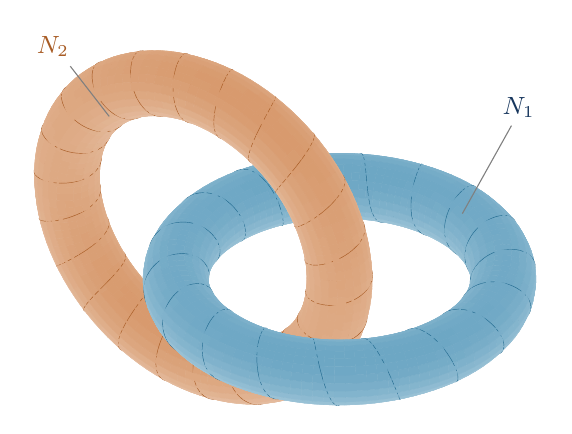
\begin{tikzpicture}[scale=1.3]
  % Generated from explicit 3D linked torus geometry; far to near.
\draw[force!85!black,line width=.16pt] (-2.16624,-0.19677)--(-2.19218,-0.20926);
\draw[force!85!black,line width=.16pt] (-2.14039,-0.18416)--(-2.16624,-0.19677);
\draw[force!85!black,line width=.16pt] (-2.19218,-0.20926)--(-2.21804,-0.22153);
\draw[force!85!black,line width=.16pt] (-2.11481,-0.17158)--(-2.14039,-0.18416);
\draw[force!85!black,line width=.16pt] (-2.21804,-0.22153)--(-2.24365,-0.23345);
\filldraw[fill=force!32!white,draw=force!32!white,line width=.07pt] (-2.15319,-0.20048)--(-2.21831,-0.12143)--(-2.28327,-0.17331)--(-2.21634,-0.25456)--cycle;
\filldraw[fill=force!31!white,draw=force!31!white,line width=.07pt] (-2.08509,-0.27698)--(-2.15319,-0.20048)--(-2.21634,-0.25456)--(-2.14633,-0.33318)--cycle;
\draw[force!85!black,line width=.16pt] (-2.08966,-0.15912)--(-2.11481,-0.17158);
\filldraw[fill=force!33!white,draw=force!33!white,line width=.07pt] (-2.09060,-0.14685)--(-2.15336,-0.07067)--(-2.21831,-0.12143)--(-2.15319,-0.20048)--cycle;
\filldraw[fill=force!33!white,draw=force!33!white,line width=.07pt] (-2.02497,-0.22057)--(-2.09060,-0.14685)--(-2.15319,-0.20048)--(-2.08509,-0.27698)--cycle;
\filldraw[fill=force!32!white,draw=force!32!white,line width=.07pt] (-2.21831,-0.12143)--(-2.28025,-0.04007)--(-2.34693,-0.08968)--(-2.28327,-0.17331)--cycle;
\filldraw[fill=force!31!white,draw=force!31!white,line width=.07pt] (-2.01422,-0.35067)--(-2.08509,-0.27698)--(-2.14633,-0.33318)--(-2.07349,-0.40892)--cycle;
\draw[force!85!black,line width=.16pt] (-2.24365,-0.23345)--(-2.26884,-0.24492);
\filldraw[fill=force!33!white,draw=force!33!white,line width=.07pt] (-2.15336,-0.07067)--(-2.21305,0.00774)--(-2.28025,-0.04007)--(-2.21831,-0.12143)--cycle;
\filldraw[fill=force!33!white,draw=force!33!white,line width=.07pt] (-1.95667,-0.29159)--(-2.02497,-0.22057)--(-2.08509,-0.27698)--(-2.01422,-0.35067)--cycle;
\draw[force!85!black,line width=.16pt] (-2.06511,-0.14692)--(-2.08966,-0.15912);
\filldraw[fill=force!32!white,draw=force!32!white,line width=.07pt] (-2.28025,-0.04007)--(-2.33881,0.04334)--(-2.40712,-0.00394)--(-2.34693,-0.08968)--cycle;
\filldraw[fill=force!31!white,draw=force!31!white,line width=.07pt] (-1.94080,-0.42133)--(-2.01422,-0.35067)--(-2.07349,-0.40892)--(-1.99803,-0.48155)--cycle;
\filldraw[fill=force!34!white,draw=force!34!white,line width=.07pt] (-2.21305,0.00774)--(-2.26948,0.08813)--(-2.33881,0.04334)--(-2.28025,-0.04007)--cycle;
\filldraw[fill=force!33!white,draw=force!33!white,line width=.07pt] (-1.88592,-0.35968)--(-1.95667,-0.29159)--(-2.01422,-0.35067)--(-1.94080,-0.42133)--cycle;
\draw[force!85!black,line width=.16pt] (-2.26884,-0.24492)--(-2.29343,-0.25583);
\draw[force!85!black,line width=.16pt] (-2.04132,-0.13509)--(-2.06511,-0.14692);
\filldraw[fill=force!31!white,draw=force!31!white,line width=.07pt] (-2.21634,-0.25456)--(-2.28327,-0.17331)--(-2.34381,-0.22275)--(-2.27573,-0.30539)--cycle;
\filldraw[fill=force!31!white,draw=force!31!white,line width=.07pt] (-2.14633,-0.33318)--(-2.21634,-0.25456)--(-2.27573,-0.30539)--(-2.20454,-0.38535)--cycle;
\filldraw[fill=force!32!white,draw=force!32!white,line width=.07pt] (-2.28327,-0.17331)--(-2.34693,-0.08968)--(-2.40855,-0.13770)--(-2.34381,-0.22275)--cycle;
\filldraw[fill=force!31!white,draw=force!31!white,line width=.07pt] (-2.07349,-0.40892)--(-2.14633,-0.33318)--(-2.20454,-0.38535)--(-2.13045,-0.46238)--cycle;
\filldraw[fill=force!33!white,draw=force!33!white,line width=.07pt] (-2.33881,0.04334)--(-2.39380,0.12855)--(-2.46364,0.08364)--(-2.40712,-0.00394)--cycle;
\filldraw[fill=force!31!white,draw=force!31!white,line width=.07pt] (-1.86508,-0.48873)--(-1.94080,-0.42133)--(-1.99803,-0.48155)--(-1.92020,-0.55083)--cycle;
\filldraw[fill=force!36!white,draw=force!36!white,line width=.07pt] (-2.03283,-0.09732)--(-2.09284,-0.02448)--(-2.15336,-0.07067)--(-2.09060,-0.14685)--cycle;
\filldraw[fill=force!36!white,draw=force!36!white,line width=.07pt] (-1.97008,-0.16780)--(-2.03283,-0.09732)--(-2.09060,-0.14685)--(-2.02497,-0.22057)--cycle;
\filldraw[fill=force!34!white,draw=force!34!white,line width=.07pt] (-2.26948,0.08813)--(-2.32248,0.17024)--(-2.39380,0.12855)--(-2.33881,0.04334)--cycle;
\draw[force!85!black,line width=.16pt] (-2.29343,-0.25583)--(-2.31727,-0.26607);
\filldraw[fill=force!33!white,draw=force!33!white,line width=.07pt] (-1.81294,-0.42464)--(-1.88592,-0.35968)--(-1.94080,-0.42133)--(-1.86508,-0.48873)--cycle;
\draw[force!85!black,line width=.16pt] (-2.01844,-0.12376)--(-2.04132,-0.13509);
\filldraw[fill=force!36!white,draw=force!36!white,line width=.07pt] (-2.09284,-0.02448)--(-2.14991,0.05049)--(-2.21305,0.00774)--(-2.15336,-0.07067)--cycle;
\filldraw[fill=force!36!white,draw=force!36!white,line width=.07pt] (-1.90477,-0.23571)--(-1.97008,-0.16780)--(-2.02497,-0.22057)--(-1.95667,-0.29159)--cycle;
\filldraw[fill=force!32!white,draw=force!32!white,line width=.07pt] (-2.34693,-0.08968)--(-2.40712,-0.00394)--(-2.46976,-0.05050)--(-2.40855,-0.13770)--cycle;
\filldraw[fill=force!31!white,draw=force!31!white,line width=.07pt] (-1.99803,-0.48155)--(-2.07349,-0.40892)--(-2.13045,-0.46238)--(-2.05371,-0.53625)--cycle;
\filldraw[fill=force!36!white,draw=force!36!white,line width=.07pt] (-2.14991,0.05049)--(-2.20387,0.12736)--(-2.26948,0.08813)--(-2.21305,0.00774)--cycle;
\filldraw[fill=force!36!white,draw=force!36!white,line width=.07pt] (-1.83712,-0.30082)--(-1.90477,-0.23571)--(-1.95667,-0.29159)--(-1.88592,-0.35968)--cycle;
\draw[force!85!black,line width=.16pt] (-2.31727,-0.26607)--(-2.34019,-0.27555);
\filldraw[fill=force!33!white,draw=force!33!white,line width=.07pt] (-2.39380,0.12855)--(-2.44505,0.21529)--(-2.51632,0.17279)--(-2.46364,0.08364)--cycle;
\filldraw[fill=force!31!white,draw=force!31!white,line width=.07pt] (-1.78727,-0.55267)--(-1.86508,-0.48873)--(-1.92020,-0.55083)--(-1.84023,-0.61655)--cycle;
\filldraw[fill=force!34!white,draw=force!34!white,line width=.07pt] (-2.32248,0.17024)--(-2.37187,0.25383)--(-2.44505,0.21529)--(-2.39380,0.12855)--cycle;
\draw[force!85!black,line width=.16pt] (-1.99662,-0.11303)--(-2.01844,-0.12376);
\filldraw[fill=force!33!white,draw=force!33!white,line width=.07pt] (-1.73796,-0.48626)--(-1.81294,-0.42464)--(-1.86508,-0.48873)--(-1.78727,-0.55267)--cycle;
\draw[force!85!black,line width=.16pt] (-1.78679,-0.55301)--(-1.80977,-0.57037);
\filldraw[fill=force!32!white,draw=force!32!white,line width=.07pt] (-2.40712,-0.00394)--(-2.46364,0.08364)--(-2.52725,0.03857)--(-2.46976,-0.05050)--cycle;
\draw[force!85!black,line width=.16pt] (-1.80977,-0.57037)--(-1.83310,-0.58720);
\filldraw[fill=force!31!white,draw=force!31!white,line width=.07pt] (-1.92020,-0.55083)--(-1.99803,-0.48155)--(-2.05371,-0.53625)--(-1.97455,-0.60671)--cycle;
\draw[force!85!black,line width=.16pt] (-1.76433,-0.53525)--(-1.78679,-0.55301);
\draw[force!85!black,line width=.16pt] (-2.41366,0.24203)--(-2.44156,0.23504);
\draw[force!85!black,line width=.16pt] (-2.44156,0.23504)--(-2.46937,0.22769);
\draw[force!85!black,line width=.16pt] (-1.83310,-0.58720)--(-1.85666,-0.60333);
\filldraw[fill=force!36!white,draw=force!36!white,line width=.07pt] (-2.20387,0.12736)--(-2.25454,0.20587)--(-2.32248,0.17024)--(-2.26948,0.08813)--cycle;
\draw[force!85!black,line width=.16pt] (-2.38589,0.24859)--(-2.41366,0.24203);
\draw[force!85!black,line width=.16pt] (-2.46937,0.22769)--(-2.49691,0.22008);
\draw[force!85!black,line width=.16pt] (-1.74252,-0.51725)--(-1.76433,-0.53525);
\filldraw[fill=force!36!white,draw=force!36!white,line width=.07pt] (-1.76735,-0.36293)--(-1.83712,-0.30082)--(-1.88592,-0.35968)--(-1.81294,-0.42464)--cycle;
\draw[force!85!black,line width=.16pt] (-1.85666,-0.60333)--(-1.88028,-0.61864);
\draw[force!85!black,line width=.16pt] (-2.35842,0.25464)--(-2.38589,0.24859);
\draw[force!85!black,line width=.16pt] (-2.49691,0.22008)--(-2.52400,0.21229);
\draw[force!85!black,line width=.16pt] (-2.34019,-0.27555)--(-2.36204,-0.28416);
\draw[force!85!black,line width=.16pt] (-1.72151,-0.49918)--(-1.74252,-0.51725);
\filldraw[fill=force!32!white,draw=force!32!white,line width=.07pt] (-2.27573,-0.30539)--(-2.34381,-0.22275)--(-2.39579,-0.26640)--(-2.32733,-0.34951)--cycle;
\filldraw[fill=force!32!white,draw=force!32!white,line width=.07pt] (-2.20454,-0.38535)--(-2.27573,-0.30539)--(-2.32733,-0.34951)--(-2.25573,-0.42993)--cycle;
\draw[force!85!black,line width=.16pt] (-1.97598,-0.10303)--(-1.99662,-0.11303);
\draw[force!85!black,line width=.16pt] (-1.88028,-0.61864)--(-1.90381,-0.63299);
\filldraw[fill=force!33!white,draw=force!33!white,line width=.07pt] (-2.46364,0.08364)--(-2.51632,0.17279)--(-2.58083,0.12924)--(-2.52725,0.03857)--cycle;
\draw[force!85!black,line width=.16pt] (-2.33144,0.26010)--(-2.35842,0.25464);
\filldraw[fill=force!33!white,draw=force!33!white,line width=.07pt] (-2.34381,-0.22275)--(-2.40855,-0.13770)--(-2.46091,-0.18087)--(-2.39579,-0.26640)--cycle;
\draw[force!85!black,line width=.16pt] (-2.52400,0.21229)--(-2.55043,0.20439);
\filldraw[fill=force!32!white,draw=force!32!white,line width=.07pt] (-2.13045,-0.46238)--(-2.20454,-0.38535)--(-2.25573,-0.42993)--(-2.18122,-0.50740)--cycle;
\filldraw[fill=force!31!white,draw=force!31!white,line width=.07pt] (-1.84023,-0.61655)--(-1.92020,-0.55083)--(-1.97455,-0.60671)--(-1.89322,-0.67355)--cycle;
\filldraw[fill=force!33!white,draw=force!33!white,line width=.07pt] (-2.44505,0.21529)--(-2.49241,0.30327)--(-2.56500,0.26323)--(-2.51632,0.17279)--cycle;
\filldraw[fill=force!35!white,draw=force!35!white,line width=.07pt] (-2.37187,0.25383)--(-2.41751,0.33862)--(-2.49241,0.30327)--(-2.44505,0.21529)--cycle;
\filldraw[fill=force!31!white,draw=force!31!white,line width=.07pt] (-1.70764,-0.61294)--(-1.78727,-0.55267)--(-1.84023,-0.61655)--(-1.75838,-0.67850)--cycle;
\filldraw[fill=force!33!white,draw=force!33!white,line width=.07pt] (-1.66122,-0.54434)--(-1.73796,-0.48626)--(-1.78727,-0.55267)--(-1.70764,-0.61294)--cycle;
\filldraw[fill=force!36!white,draw=force!36!white,line width=.07pt] (-2.25454,0.20587)--(-2.30177,0.28579)--(-2.37187,0.25383)--(-2.32248,0.17024)--cycle;
\draw[force!85!black,line width=.16pt] (-1.70141,-0.48118)--(-1.72151,-0.49918);
\filldraw[fill=force!36!white,draw=force!36!white,line width=.07pt] (-1.69566,-0.42184)--(-1.76735,-0.36293)--(-1.81294,-0.42464)--(-1.73796,-0.48626)--cycle;
\draw[force!85!black,line width=.16pt] (-1.90381,-0.63299)--(-1.92709,-0.64626);
\filldraw[fill=force!39!white,draw=force!39!white,line width=.07pt] (-1.98382,-0.05526)--(-2.04087,0.01400)--(-2.09284,-0.02448)--(-2.03283,-0.09732)--cycle;
\filldraw[fill=force!39!white,draw=force!39!white,line width=.07pt] (-1.92415,-0.12227)--(-1.98382,-0.05526)--(-2.03283,-0.09732)--(-1.97008,-0.16780)--cycle;
\filldraw[fill=force!33!white,draw=force!33!white,line width=.07pt] (-2.40855,-0.13770)--(-2.46976,-0.05050)--(-2.52247,-0.09317)--(-2.46091,-0.18087)--cycle;
\draw[force!85!black,line width=.16pt] (-2.30514,0.26490)--(-2.33144,0.26010);
\filldraw[fill=force!32!white,draw=force!32!white,line width=.07pt] (-2.05371,-0.53625)--(-2.13045,-0.46238)--(-2.18122,-0.50740)--(-2.10404,-0.58169)--cycle;
\draw[force!85!black,line width=.16pt] (-2.55043,0.20439)--(-2.57603,0.19649);
\filldraw[fill=force!39!white,draw=force!39!white,line width=.07pt] (-2.04087,0.01400)--(-2.09513,0.08528)--(-2.14991,0.05049)--(-2.09284,-0.02448)--cycle;
\filldraw[fill=force!39!white,draw=force!39!white,line width=.07pt] (-1.86206,-0.18684)--(-1.92415,-0.12227)--(-1.97008,-0.16780)--(-1.90477,-0.23571)--cycle;
\draw[force!85!black,line width=.16pt] (-2.36204,-0.28416)--(-2.38267,-0.29183);
\draw[force!85!black,line width=.16pt] (-1.68235,-0.46341)--(-1.70141,-0.48118);
\draw[force!85!black,line width=.16pt] (-1.95666,-0.09385)--(-1.97598,-0.10303);
\filldraw[fill=force!40!white,draw=force!40!white,line width=.07pt] (-2.09513,0.08528)--(-2.14644,0.15836)--(-2.20387,0.12736)--(-2.14991,0.05049)--cycle;
\filldraw[fill=force!39!white,draw=force!39!white,line width=.07pt] (-1.79774,-0.24874)--(-1.86206,-0.18684)--(-1.90477,-0.23571)--(-1.83712,-0.30082)--cycle;
\draw[force!85!black,line width=.16pt] (-1.92709,-0.64626)--(-1.94998,-0.65833);
\draw[force!85!black,line width=.16pt] (-2.27969,0.26896)--(-2.30514,0.26490);
\filldraw[fill=force!33!white,draw=force!33!white,line width=.07pt] (-2.51632,0.17279)--(-2.56500,0.26323)--(-2.63033,0.22121)--(-2.58083,0.12924)--cycle;
\draw[force!85!black,line width=.16pt] (-2.57603,0.19649)--(-2.60063,0.18865);
\filldraw[fill=force!33!white,draw=force!33!white,line width=.07pt] (-2.46976,-0.05050)--(-2.52725,0.03857)--(-2.58028,-0.00359)--(-2.52247,-0.09317)--cycle;
\filldraw[fill=force!31!white,draw=force!31!white,line width=.07pt] (-1.75838,-0.67850)--(-1.84023,-0.61655)--(-1.89322,-0.67355)--(-1.80998,-0.73655)--cycle;
\filldraw[fill=force!31!white,draw=force!31!white,line width=.07pt] (-1.97455,-0.60671)--(-2.05371,-0.53625)--(-2.10404,-0.58169)--(-2.02443,-0.65255)--cycle;
\filldraw[fill=force!37!white,draw=force!37!white,line width=.07pt] (-2.30177,0.28579)--(-2.34540,0.36687)--(-2.41751,0.33862)--(-2.37187,0.25383)--cycle;
\filldraw[fill=force!36!white,draw=force!36!white,line width=.07pt] (-1.62228,-0.47738)--(-1.69566,-0.42184)--(-1.73796,-0.48626)--(-1.66122,-0.54434)--cycle;
\filldraw[fill=force!35!white,draw=force!35!white,line width=.07pt] (-2.41751,0.33862)--(-2.45924,0.42435)--(-2.53571,0.39223)--(-2.49241,0.30327)--cycle;
\filldraw[fill=force!34!white,draw=force!34!white,line width=.07pt] (-2.49241,0.30327)--(-2.53571,0.39223)--(-2.60951,0.35466)--(-2.56500,0.26323)--cycle;
\filldraw[fill=force!33!white,draw=force!33!white,line width=.07pt] (-1.58296,-0.59871)--(-1.66122,-0.54434)--(-1.70764,-0.61294)--(-1.62643,-0.66936)--cycle;
\filldraw[fill=force!31!white,draw=force!31!white,line width=.07pt] (-1.62643,-0.66936)--(-1.70764,-0.61294)--(-1.75838,-0.67850)--(-1.67491,-0.73648)--cycle;
\draw[force!85!black,line width=.16pt] (-1.66445,-0.44603)--(-1.68235,-0.46341);
\filldraw[fill=force!40!white,draw=force!40!white,line width=.07pt] (-2.14644,0.15836)--(-2.19461,0.23301)--(-2.25454,0.20587)--(-2.20387,0.12736)--cycle;
\filldraw[fill=force!39!white,draw=force!39!white,line width=.07pt] (-1.73140,-0.30779)--(-1.79774,-0.24874)--(-1.83712,-0.30082)--(-1.76735,-0.36293)--cycle;
\draw[force!85!black,line width=.16pt] (-2.38267,-0.29183)--(-2.40195,-0.29848);
\draw[force!85!black,line width=.16pt] (-1.94998,-0.65833)--(-1.97233,-0.66908);
\draw[force!85!black,line width=.16pt] (-2.25526,0.27222)--(-2.27969,0.26896);
\draw[force!85!black,line width=.16pt] (-1.93877,-0.08560)--(-1.95666,-0.09385);
\draw[force!85!black,line width=.16pt] (-2.60063,0.18865)--(-2.62404,0.18097);
\filldraw[fill=force!34!white,draw=force!34!white,line width=.07pt] (-2.52725,0.03857)--(-2.58083,0.12924)--(-2.63417,0.08760)--(-2.58028,-0.00359)--cycle;
\filldraw[fill=force!31!white,draw=force!31!white,line width=.07pt] (-1.89322,-0.67355)--(-1.97455,-0.60671)--(-2.02443,-0.65255)--(-1.94263,-0.71977)--cycle;
\draw[force!85!black,line width=.16pt] (-1.64779,-0.42920)--(-1.66445,-0.44603);
\filldraw[fill=force!40!white,draw=force!40!white,line width=.07pt] (-2.19461,0.23301)--(-2.23952,0.30900)--(-2.30177,0.28579)--(-2.25454,0.20587)--cycle;
\filldraw[fill=force!37!white,draw=force!37!white,line width=.07pt] (-2.34540,0.36687)--(-2.38531,0.44884)--(-2.45924,0.42435)--(-2.41751,0.33862)--cycle;
\filldraw[fill=force!39!white,draw=force!39!white,line width=.07pt] (-1.66324,-0.36381)--(-1.73140,-0.30779)--(-1.76735,-0.36293)--(-1.69566,-0.42184)--cycle;
\filldraw[fill=force!34!white,draw=force!34!white,line width=.07pt] (-2.56500,0.26323)--(-2.60951,0.35466)--(-2.67560,0.31421)--(-2.63033,0.22121)--cycle;
\filldraw[fill=force!36!white,draw=force!36!white,line width=.07pt] (-1.54745,-0.52936)--(-1.62228,-0.47738)--(-1.66122,-0.54434)--(-1.58296,-0.59871)--cycle;
\filldraw[fill=force!31!white,draw=force!31!white,line width=.07pt] (-1.67491,-0.73648)--(-1.75838,-0.67850)--(-1.80998,-0.73655)--(-1.72508,-0.79552)--cycle;
\draw[force!85!black,line width=.16pt] (-1.97233,-0.66908)--(-1.99399,-0.67843);
\draw[force!85!black,line width=.16pt] (-2.23202,0.27462)--(-2.25526,0.27222);
\draw[force!85!black,line width=.16pt] (-2.62404,0.18097)--(-2.64611,0.17353);
\filldraw[fill=force!34!white,draw=force!34!white,line width=.07pt] (-2.32733,-0.34951)--(-2.39579,-0.26640)--(-2.43569,-0.30128)--(-2.36761,-0.38392)--cycle;
\filldraw[fill=force!34!white,draw=force!34!white,line width=.07pt] (-2.25573,-0.42993)--(-2.32733,-0.34951)--(-2.36761,-0.38392)--(-2.29642,-0.46388)--cycle;
\draw[force!85!black,line width=.16pt] (-2.40195,-0.29848)--(-2.41975,-0.30404);
\filldraw[fill=force!35!white,draw=force!35!white,line width=.07pt] (-2.45924,0.42435)--(-2.49694,0.51075)--(-2.57484,0.48188)--(-2.53571,0.39223)--cycle;
\filldraw[fill=force!34!white,draw=force!34!white,line width=.07pt] (-2.53571,0.39223)--(-2.57484,0.48188)--(-2.64972,0.44681)--(-2.60951,0.35466)--cycle;
\filldraw[fill=force!33!white,draw=force!33!white,line width=.07pt] (-1.50342,-0.64919)--(-1.58296,-0.59871)--(-1.62643,-0.66936)--(-1.54390,-0.72173)--cycle;
\filldraw[fill=force!31!white,draw=force!31!white,line width=.07pt] (-1.54390,-0.72173)--(-1.62643,-0.66936)--(-1.67491,-0.73648)--(-1.59008,-0.79032)--cycle;
\filldraw[fill=force!35!white,draw=force!35!white,line width=.07pt] (-2.39579,-0.26640)--(-2.46091,-0.18087)--(-2.50044,-0.21623)--(-2.43569,-0.30128)--cycle;
\draw[force!85!black,line width=.16pt] (-1.92242,-0.07839)--(-1.93877,-0.08560);
\filldraw[fill=force!34!white,draw=force!34!white,line width=.07pt] (-2.18122,-0.50740)--(-2.25573,-0.42993)--(-2.29642,-0.46388)--(-2.22234,-0.54091)--cycle;
\draw[force!85!black,line width=.16pt] (-1.63248,-0.41306)--(-1.64779,-0.42920);
\filldraw[fill=force!34!white,draw=force!34!white,line width=.07pt] (-2.58083,0.12924)--(-2.63033,0.22121)--(-2.68395,0.18010)--(-2.63417,0.08760)--cycle;
\filldraw[fill=force!31!white,draw=force!31!white,line width=.07pt] (-1.80998,-0.73655)--(-1.89322,-0.67355)--(-1.94263,-0.71977)--(-1.85891,-0.78314)--cycle;
\filldraw[fill=force!40!white,draw=force!40!white,line width=.07pt] (-2.23952,0.30900)--(-2.28100,0.38608)--(-2.34540,0.36687)--(-2.30177,0.28579)--cycle;
\filldraw[fill=force!39!white,draw=force!39!white,line width=.07pt] (-1.59347,-0.41661)--(-1.66324,-0.36381)--(-1.69566,-0.42184)--(-1.62228,-0.47738)--cycle;
\filldraw[fill=force!35!white,draw=force!35!white,line width=.07pt] (-2.46091,-0.18087)--(-2.52247,-0.09317)--(-2.56165,-0.12903)--(-2.50044,-0.21623)--cycle;
\filldraw[fill=force!34!white,draw=force!34!white,line width=.07pt] (-2.10404,-0.58169)--(-2.18122,-0.50740)--(-2.22234,-0.54091)--(-2.14559,-0.61478)--cycle;
\draw[force!85!black,line width=.16pt] (-2.21012,0.27610)--(-2.23202,0.27462);
\draw[force!85!black,line width=.16pt] (-1.99399,-0.67843)--(-2.01481,-0.68628);
\filldraw[fill=force!44!white,draw=force!44!white,line width=.07pt] (-1.94690,-0.02354)--(-2.00100,0.04213)--(-2.04087,0.01400)--(-1.98382,-0.05526)--cycle;
\filldraw[fill=force!44!white,draw=force!44!white,line width=.07pt] (-1.89032,-0.08708)--(-1.94690,-0.02354)--(-1.98382,-0.05526)--(-1.92415,-0.12227)--cycle;
\draw[force!85!black,line width=.16pt] (-2.64611,0.17353)--(-2.66669,0.16641);
\filldraw[fill=force!44!white,draw=force!44!white,line width=.07pt] (-2.00100,0.04213)--(-2.05245,0.10972)--(-2.09513,0.08528)--(-2.04087,0.01400)--cycle;
\filldraw[fill=force!44!white,draw=force!44!white,line width=.07pt] (-1.83145,-0.14830)--(-1.89032,-0.08708)--(-1.92415,-0.12227)--(-1.86206,-0.18684)--cycle;
\filldraw[fill=force!37!white,draw=force!37!white,line width=.07pt] (-2.38531,0.44884)--(-2.42135,0.53145)--(-2.49694,0.51075)--(-2.45924,0.42435)--cycle;
\filldraw[fill=force!36!white,draw=force!36!white,line width=.07pt] (-1.47140,-0.57763)--(-1.54745,-0.52936)--(-1.58296,-0.59871)--(-1.50342,-0.64919)--cycle;
\filldraw[fill=force!34!white,draw=force!34!white,line width=.07pt] (-2.60951,0.35466)--(-2.64972,0.44681)--(-2.71650,0.40793)--(-2.67560,0.31421)--cycle;
\draw[force!85!black,line width=.16pt] (-2.41975,-0.30404)--(-2.43596,-0.30843);
\filldraw[fill=force!31!white,draw=force!31!white,line width=.07pt] (-1.59008,-0.79032)--(-1.67491,-0.73648)--(-1.72508,-0.79552)--(-1.63881,-0.85028)--cycle;
\filldraw[fill=force!35!white,draw=force!35!white,line width=.07pt] (-2.52247,-0.09317)--(-2.58028,-0.00359)--(-2.61913,-0.03996)--(-2.56165,-0.12903)--cycle;
\draw[force!85!black,line width=.16pt] (-1.61860,-0.39777)--(-1.63248,-0.41306);
\filldraw[fill=force!44!white,draw=force!44!white,line width=.07pt] (-2.05245,0.10972)--(-2.10110,0.17902)--(-2.14644,0.15836)--(-2.09513,0.08528)--cycle;
\filldraw[fill=force!34!white,draw=force!34!white,line width=.07pt] (-2.02443,-0.65255)--(-2.10404,-0.58169)--(-2.14559,-0.61478)--(-2.06643,-0.68524)--cycle;
\filldraw[fill=force!44!white,draw=force!44!white,line width=.07pt] (-1.77046,-0.20700)--(-1.83145,-0.14830)--(-1.86206,-0.18684)--(-1.79774,-0.24874)--cycle;
\draw[force!85!black,line width=.16pt] (-1.90769,-0.07229)--(-1.92242,-0.07839);
\filldraw[fill=force!36!white,draw=force!36!white,line width=.07pt] (-2.49694,0.51075)--(-2.53049,0.59755)--(-2.60965,0.57195)--(-2.57484,0.48188)--cycle;
\filldraw[fill=force!40!white,draw=force!40!white,line width=.07pt] (-2.28100,0.38608)--(-2.31894,0.46402)--(-2.38531,0.44884)--(-2.34540,0.36687)--cycle;
\draw[force!85!black,line width=.16pt] (-2.18970,0.27662)--(-2.21012,0.27610);
\draw[force!85!black,line width=.16pt] (-2.01481,-0.68628)--(-2.03468,-0.69256);
\filldraw[fill=force!35!white,draw=force!35!white,line width=.07pt] (-2.63033,0.22121)--(-2.67560,0.31421)--(-2.72948,0.27362)--(-2.68395,0.18010)--cycle;
\filldraw[fill=force!33!white,draw=force!33!white,line width=.07pt] (-1.42285,-0.69562)--(-1.50342,-0.64919)--(-1.54390,-0.72173)--(-1.46030,-0.76991)--cycle;
\filldraw[fill=force!35!white,draw=force!35!white,line width=.07pt] (-2.57484,0.48188)--(-2.60965,0.57195)--(-2.68550,0.53939)--(-2.64972,0.44681)--cycle;
\filldraw[fill=force!39!white,draw=force!39!white,line width=.07pt] (-1.52232,-0.46604)--(-1.59347,-0.41661)--(-1.62228,-0.47738)--(-1.54745,-0.52936)--cycle;
\filldraw[fill=force!31!white,draw=force!31!white,line width=.07pt] (-1.72508,-0.79552)--(-1.80998,-0.73655)--(-1.85891,-0.78314)--(-1.77354,-0.84244)--cycle;
\filldraw[fill=force!31!white,draw=force!31!white,line width=.07pt] (-1.46030,-0.76991)--(-1.54390,-0.72173)--(-1.59008,-0.79032)--(-1.50415,-0.83984)--cycle;
\draw[force!85!black,line width=.16pt] (-2.66669,0.16641)--(-2.68563,0.15968);
\filldraw[fill=force!44!white,draw=force!44!white,line width=.07pt] (-2.10110,0.17902)--(-2.14678,0.24981)--(-2.19461,0.23301)--(-2.14644,0.15836)--cycle;
\filldraw[fill=force!44!white,draw=force!44!white,line width=.07pt] (-1.70755,-0.26300)--(-1.77046,-0.20700)--(-1.79774,-0.24874)--(-1.73140,-0.30779)--cycle;
\filldraw[fill=force!36!white,draw=force!36!white,line width=.07pt] (-2.58028,-0.00359)--(-2.63417,0.08760)--(-2.67271,0.05071)--(-2.61913,-0.03996)--cycle;
\filldraw[fill=force!33!white,draw=force!33!white,line width=.07pt] (-1.94263,-0.71977)--(-2.02443,-0.65255)--(-2.06643,-0.68524)--(-1.98510,-0.75208)--cycle;
\draw[force!85!black,line width=.16pt] (-1.60621,-0.38347)--(-1.61860,-0.39777);
\draw[force!85!black,line width=.16pt] (-2.43596,-0.30843)--(-2.45046,-0.31162);
\filldraw[fill=force!37!white,draw=force!37!white,line width=.07pt] (-2.42135,0.53145)--(-2.45343,0.61444)--(-2.53049,0.59755)--(-2.49694,0.51075)--cycle;
\filldraw[fill=force!43!white,draw=force!43!white,line width=.07pt] (-2.14678,0.24981)--(-2.18936,0.32186)--(-2.23952,0.30900)--(-2.19461,0.23301)--cycle;
\draw[force!85!black,line width=.16pt] (-1.89465,-0.06739)--(-1.90769,-0.07229);
\filldraw[fill=force!44!white,draw=force!44!white,line width=.07pt] (-1.64291,-0.31612)--(-1.70755,-0.26300)--(-1.73140,-0.30779)--(-1.66324,-0.36381)--cycle;
\filldraw[fill=force!36!white,draw=force!36!white,line width=.07pt] (-1.39437,-0.62202)--(-1.47140,-0.57763)--(-1.50342,-0.64919)--(-1.42285,-0.69562)--cycle;
\draw[force!85!black,line width=.16pt] (-2.17089,0.27612)--(-2.18970,0.27662);
\draw[force!85!black,line width=.16pt] (-2.03468,-0.69256)--(-2.05345,-0.69720);
\filldraw[fill=force!35!white,draw=force!35!white,line width=.07pt] (-2.64972,0.44681)--(-2.68550,0.53939)--(-2.75289,0.50208)--(-2.71650,0.40793)--cycle;
\draw[force!85!black,line width=.16pt] (-2.68563,0.15968)--(-2.70281,0.15341);
\filldraw[fill=force!31!white,draw=force!31!white,line width=.07pt] (-1.50415,-0.83984)--(-1.59008,-0.79032)--(-1.63881,-0.85028)--(-1.55142,-0.90064)--cycle;
\filldraw[fill=force!40!white,draw=force!40!white,line width=.07pt] (-2.31894,0.46402)--(-2.35322,0.54256)--(-2.42135,0.53145)--(-2.38531,0.44884)--cycle;
\filldraw[fill=force!39!white,draw=force!39!white,line width=.07pt] (-1.45001,-0.51193)--(-1.52232,-0.46604)--(-1.54745,-0.52936)--(-1.47140,-0.57763)--cycle;
\filldraw[fill=force!36!white,draw=force!36!white,line width=.07pt] (-2.67560,0.31421)--(-2.71650,0.40793)--(-2.77061,0.36788)--(-2.72948,0.27362)--cycle;
\filldraw[fill=force!36!white,draw=force!36!white,line width=.07pt] (-2.63417,0.08760)--(-2.68395,0.18010)--(-2.72221,0.14268)--(-2.67271,0.05071)--cycle;
\filldraw[fill=force!32!white,draw=force!32!white,line width=.07pt] (-1.63881,-0.85028)--(-1.72508,-0.79552)--(-1.77354,-0.84244)--(-1.68677,-0.89751)--cycle;
\filldraw[fill=force!33!white,draw=force!33!white,line width=.07pt] (-1.85891,-0.78314)--(-1.94263,-0.71977)--(-1.98510,-0.75208)--(-1.90186,-0.81508)--cycle;
\filldraw[fill=force!36!white,draw=force!36!white,line width=.07pt] (-2.53049,0.59755)--(-2.55979,0.68447)--(-2.64005,0.66214)--(-2.60965,0.57195)--cycle;
\draw[force!85!black,line width=.16pt] (-1.59538,-0.37028)--(-1.60621,-0.38347);
\filldraw[fill=force!43!white,draw=force!43!white,line width=.07pt] (-2.18936,0.32186)--(-2.22870,0.39496)--(-2.28100,0.38608)--(-2.23952,0.30900)--cycle;
\filldraw[fill=force!44!white,draw=force!44!white,line width=.07pt] (-1.57676,-0.36619)--(-1.64291,-0.31612)--(-1.66324,-0.36381)--(-1.59347,-0.41661)--cycle;
\filldraw[fill=force!33!white,draw=force!33!white,line width=.07pt] (-1.34152,-0.73786)--(-1.42285,-0.69562)--(-1.46030,-0.76991)--(-1.37590,-0.81374)--cycle;
\filldraw[fill=force!37!white,draw=force!37!white,line width=.07pt] (-2.36761,-0.38392)--(-2.43569,-0.30128)--(-2.46078,-0.32502)--(-2.39384,-0.40627)--cycle;
\filldraw[fill=force!37!white,draw=force!37!white,line width=.07pt] (-2.29642,-0.46388)--(-2.36761,-0.38392)--(-2.39384,-0.40627)--(-2.32384,-0.48489)--cycle;
\filldraw[fill=force!35!white,draw=force!35!white,line width=.07pt] (-2.60965,0.57195)--(-2.64005,0.66214)--(-2.71675,0.63209)--(-2.68550,0.53939)--cycle;
\draw[force!85!black,line width=.16pt] (-2.45046,-0.31162)--(-2.46319,-0.31354);
\filldraw[fill=force!31!white,draw=force!31!white,line width=.07pt] (-1.37590,-0.81374)--(-1.46030,-0.76991)--(-1.50415,-0.83984)--(-1.41740,-0.88489)--cycle;
\filldraw[fill=force!38!white,draw=force!38!white,line width=.07pt] (-2.43569,-0.30128)--(-2.50044,-0.21623)--(-2.52444,-0.24139)--(-2.46078,-0.32502)--cycle;
\filldraw[fill=force!37!white,draw=force!37!white,line width=.07pt] (-2.22234,-0.54091)--(-2.29642,-0.46388)--(-2.32384,-0.48489)--(-2.25099,-0.56064)--cycle;
\draw[force!85!black,line width=.16pt] (-2.15379,0.27457)--(-2.17089,0.27612);
\draw[force!85!black,line width=.16pt] (-2.05345,-0.69720)--(-2.07101,-0.70016);
\draw[force!85!black,line width=.16pt] (-1.88339,-0.06377)--(-1.89465,-0.06739);
\draw[force!85!black,line width=.16pt] (-2.70281,0.15341)--(-2.71811,0.14769);
\filldraw[fill=force!38!white,draw=force!38!white,line width=.07pt] (-2.50044,-0.21623)--(-2.56165,-0.12903)--(-2.58462,-0.15565)--(-2.52444,-0.24139)--cycle;
\filldraw[fill=force!37!white,draw=force!37!white,line width=.07pt] (-2.14559,-0.61478)--(-2.22234,-0.54091)--(-2.25099,-0.56064)--(-2.17554,-0.63326)--cycle;
\filldraw[fill=force!38!white,draw=force!38!white,line width=.07pt] (-2.45343,0.61444)--(-2.48144,0.69755)--(-2.55979,0.68447)--(-2.53049,0.59755)--cycle;
\draw[force!85!black,line width=.16pt] (-1.36220,-0.81214)--(-1.38104,-0.83390);
\filldraw[fill=force!36!white,draw=force!36!white,line width=.07pt] (-1.31660,-0.66241)--(-1.39437,-0.62202)--(-1.42285,-0.69562)--(-1.34152,-0.73786)--cycle;
\draw[force!85!black,line width=.16pt] (-1.38104,-0.83390)--(-1.40071,-0.85493);
\filldraw[fill=force!40!white,draw=force!40!white,line width=.07pt] (-2.35322,0.54256)--(-2.38372,0.62147)--(-2.45343,0.61444)--(-2.42135,0.53145)--cycle;
\draw[force!85!black,line width=.16pt] (-2.58552,0.69082)--(-2.61426,0.68989);
\draw[force!85!black,line width=.16pt] (-1.34431,-0.78981)--(-1.36220,-0.81214);
\draw[force!85!black,line width=.16pt] (-2.55684,0.69092)--(-2.58552,0.69082);
\draw[force!85!black,line width=.16pt] (-1.40071,-0.85493)--(-1.42110,-0.87504);
\filldraw[fill=force!48!white,draw=force!48!white,line width=.07pt] (-1.92459,-0.00432)--(-1.97594,0.05801)--(-2.00100,0.04213)--(-1.94690,-0.02354)--cycle;
\filldraw[fill=force!48!white,draw=force!48!white,line width=.07pt] (-1.87089,-0.06463)--(-1.92459,-0.00432)--(-1.94690,-0.02354)--(-1.89032,-0.08708)--cycle;
\filldraw[fill=force!39!white,draw=force!39!white,line width=.07pt] (-1.37677,-0.55414)--(-1.45001,-0.51193)--(-1.47140,-0.57763)--(-1.39437,-0.62202)--cycle;
\draw[force!85!black,line width=.16pt] (-2.61426,0.68989)--(-2.64286,0.68817);
\filldraw[fill=force!43!white,draw=force!43!white,line width=.07pt] (-2.22870,0.39496)--(-2.26468,0.46886)--(-2.31894,0.46402)--(-2.28100,0.38608)--cycle;
\filldraw[fill=force!37!white,draw=force!37!white,line width=.07pt] (-2.68395,0.18010)--(-2.72948,0.27362)--(-2.76748,0.23567)--(-2.72221,0.14268)--cycle;
\filldraw[fill=force!44!white,draw=force!44!white,line width=.07pt] (-1.50929,-0.41305)--(-1.57676,-0.36619)--(-1.59347,-0.41661)--(-1.52232,-0.46604)--cycle;
\draw[force!85!black,line width=.16pt] (-2.52844,0.69016)--(-2.55684,0.69092);
\filldraw[fill=force!34!white,draw=force!34!white,line width=.07pt] (-1.77354,-0.84244)--(-1.85891,-0.78314)--(-1.90186,-0.81508)--(-1.81697,-0.87405)--cycle;
\draw[force!85!black,line width=.16pt] (-1.58613,-0.35834)--(-1.59538,-0.37028);
\filldraw[fill=force!48!white,draw=force!48!white,line width=.07pt] (-1.97594,0.05801)--(-2.02478,0.12217)--(-2.05245,0.10972)--(-2.00100,0.04213)--cycle;
\filldraw[fill=force!49!white,draw=force!49!white,line width=.07pt] (-1.81501,-0.12274)--(-1.87089,-0.06463)--(-1.89032,-0.08708)--(-1.83145,-0.14830)--cycle;
\draw[force!85!black,line width=.16pt] (-1.32748,-0.76710)--(-1.34431,-0.78981);
\draw[force!85!black,line width=.16pt] (-1.42110,-0.87504)--(-1.44208,-0.89409);
\draw[force!85!black,line width=.16pt] (-2.64286,0.68817)--(-2.67112,0.68570);
\filldraw[fill=force!36!white,draw=force!36!white,line width=.07pt] (-2.68550,0.53939)--(-2.71675,0.63209)--(-2.78466,0.59636)--(-2.75289,0.50208)--cycle;
\filldraw[fill=force!39!white,draw=force!39!white,line width=.07pt] (-2.56165,-0.12903)--(-2.61913,-0.03996)--(-2.64115,-0.06807)--(-2.58462,-0.15565)--cycle;
\filldraw[fill=force!31!white,draw=force!31!white,line width=.07pt] (-1.41740,-0.88489)--(-1.50415,-0.83984)--(-1.55142,-0.90064)--(-1.46319,-0.94646)--cycle;
\filldraw[fill=force!37!white,draw=force!37!white,line width=.07pt] (-2.06643,-0.68524)--(-2.14559,-0.61478)--(-2.17554,-0.63326)--(-2.09770,-0.70255)--cycle;
\draw[force!85!black,line width=.16pt] (-2.50050,0.68850)--(-2.52844,0.69016);
\filldraw[fill=force!36!white,draw=force!36!white,line width=.07pt] (-2.71650,0.40793)--(-2.75289,0.50208)--(-2.80721,0.46257)--(-2.77061,0.36788)--cycle;
\filldraw[fill=force!48!white,draw=force!48!white,line width=.07pt] (-2.02478,0.12217)--(-2.07095,0.18794)--(-2.10110,0.17902)--(-2.05245,0.10972)--cycle;
\draw[force!85!black,line width=.16pt] (-2.46319,-0.31354)--(-2.47405,-0.31417);
\draw[force!85!black,line width=.16pt] (-1.31180,-0.74420)--(-1.32748,-0.76710);
\filldraw[fill=force!49!white,draw=force!49!white,line width=.07pt] (-1.75713,-0.17845)--(-1.81501,-0.12274)--(-1.83145,-0.14830)--(-1.77046,-0.20700)--cycle;
\filldraw[fill=force!32!white,draw=force!32!white,line width=.07pt] (-1.55142,-0.90064)--(-1.63881,-0.85028)--(-1.68677,-0.89751)--(-1.59888,-0.94816)--cycle;
\draw[force!85!black,line width=.16pt] (-2.67112,0.68570)--(-2.69884,0.68253);
\draw[force!85!black,line width=.16pt] (-2.13853,0.27193)--(-2.15379,0.27457);
\draw[force!85!black,line width=.16pt] (-2.07101,-0.70016)--(-2.08725,-0.70139);
\draw[force!85!black,line width=.16pt] (-1.44208,-0.89409)--(-1.46351,-0.91190);
\draw[force!85!black,line width=.16pt] (-1.87393,-0.06150)--(-1.88339,-0.06377);
\draw[force!85!black,line width=.16pt] (-2.47324,0.68593)--(-2.50050,0.68850);
\draw[force!85!black,line width=.16pt] (-2.71811,0.14769)--(-2.73143,0.14257);
\filldraw[fill=force!36!white,draw=force!36!white,line width=.07pt] (-2.55979,0.68447)--(-2.58473,0.77124)--(-2.66593,0.75219)--(-2.64005,0.66214)--cycle;
\draw[force!85!black,line width=.16pt] (-1.29735,-0.72129)--(-1.31180,-0.74420);
\draw[force!85!black,line width=.16pt] (-2.69884,0.68253)--(-2.72580,0.67870);
\draw[force!85!black,line width=.16pt] (-1.46351,-0.91190)--(-1.48526,-0.92835);
\filldraw[fill=force!48!white,draw=force!48!white,line width=.07pt] (-2.07095,0.18794)--(-2.11431,0.25513)--(-2.14678,0.24981)--(-2.10110,0.17902)--cycle;
\filldraw[fill=force!33!white,draw=force!33!white,line width=.07pt] (-1.25967,-0.77577)--(-1.34152,-0.73786)--(-1.37590,-0.81374)--(-1.29097,-0.85308)--cycle;
\filldraw[fill=force!49!white,draw=force!49!white,line width=.07pt] (-1.69742,-0.23160)--(-1.75713,-0.17845)--(-1.77046,-0.20700)--(-1.70755,-0.26300)--cycle;
\filldraw[fill=force!36!white,draw=force!36!white,line width=.07pt] (-2.64005,0.66214)--(-2.66593,0.75219)--(-2.74335,0.72464)--(-2.71675,0.63209)--cycle;
\filldraw[fill=force!39!white,draw=force!39!white,line width=.07pt] (-2.61913,-0.03996)--(-2.67271,0.05071)--(-2.69383,0.02108)--(-2.64115,-0.06807)--cycle;
\filldraw[fill=force!32!white,draw=force!32!white,line width=.07pt] (-1.29097,-0.85308)--(-1.37590,-0.81374)--(-1.41740,-0.88489)--(-1.33010,-0.92533)--cycle;
\filldraw[fill=force!37!white,draw=force!37!white,line width=.07pt] (-1.98510,-0.75208)--(-2.06643,-0.68524)--(-2.09770,-0.70255)--(-2.01773,-0.76826)--cycle;
\draw[force!85!black,line width=.16pt] (-2.44685,0.68243)--(-2.47324,0.68593);
\filldraw[fill=force!43!white,draw=force!43!white,line width=.07pt] (-2.26468,0.46886)--(-2.29718,0.54334)--(-2.35322,0.54256)--(-2.31894,0.46402)--cycle;
\filldraw[fill=force!44!white,draw=force!44!white,line width=.07pt] (-1.44073,-0.45657)--(-1.50929,-0.41305)--(-1.52232,-0.46604)--(-1.45001,-0.51193)--cycle;
\draw[force!85!black,line width=.16pt] (-1.57851,-0.34777)--(-1.58613,-0.35834);
\draw[force!85!black,line width=.16pt] (-1.28422,-0.69855)--(-1.29735,-0.72129);
\draw[force!85!black,line width=.16pt] (-2.72580,0.67870)--(-2.75183,0.67428);
\draw[force!85!black,line width=.16pt] (-1.48526,-0.92835)--(-1.50720,-0.94328);
\filldraw[fill=force!38!white,draw=force!38!white,line width=.07pt] (-2.72948,0.27362)--(-2.77061,0.36788)--(-2.80838,0.32939)--(-2.76748,0.23567)--cycle;
\filldraw[fill=force!40!white,draw=force!40!white,line width=.07pt] (-2.38372,0.62147)--(-2.41035,0.70049)--(-2.48144,0.69755)--(-2.45343,0.61444)--cycle;
\filldraw[fill=force!38!white,draw=force!38!white,line width=.07pt] (-2.48144,0.69755)--(-2.50529,0.78052)--(-2.58473,0.77124)--(-2.55979,0.68447)--cycle;
\filldraw[fill=force!34!white,draw=force!34!white,line width=.07pt] (-1.68677,-0.89751)--(-1.77354,-0.84244)--(-1.81697,-0.87405)--(-1.73069,-0.92881)--cycle;
\filldraw[fill=force!39!white,draw=force!39!white,line width=.07pt] (-1.30283,-0.59254)--(-1.37677,-0.55414)--(-1.39437,-0.62202)--(-1.31660,-0.66241)--cycle;
\filldraw[fill=force!48!white,draw=force!48!white,line width=.07pt] (-2.11431,0.25513)--(-2.15472,0.32351)--(-2.18936,0.32186)--(-2.14678,0.24981)--cycle;
\filldraw[fill=force!49!white,draw=force!49!white,line width=.07pt] (-1.63607,-0.28201)--(-1.69742,-0.23160)--(-1.70755,-0.26300)--(-1.64291,-0.31612)--cycle;
\draw[force!85!black,line width=.16pt] (-2.12518,0.26819)--(-2.13853,0.27193);
\draw[force!85!black,line width=.16pt] (-2.08725,-0.70139)--(-2.10207,-0.70086);
\filldraw[fill=force!36!white,draw=force!36!white,line width=.07pt] (-1.23833,-0.69866)--(-1.31660,-0.66241)--(-1.34152,-0.73786)--(-1.25967,-0.77577)--cycle;
\draw[force!85!black,line width=.16pt] (-2.42150,0.67799)--(-2.44685,0.68243);
\draw[force!85!black,line width=.16pt] (-2.47405,-0.31417)--(-2.48298,-0.31347);
\draw[force!85!black,line width=.16pt] (-1.86632,-0.06062)--(-1.87393,-0.06150);
\draw[force!85!black,line width=.16pt] (-1.27246,-0.67617)--(-1.28422,-0.69855);
\draw[force!85!black,line width=.16pt] (-1.50720,-0.94328)--(-1.52918,-0.95658);
\draw[force!85!black,line width=.16pt] (-2.75183,0.67428)--(-2.77673,0.66933);
\draw[force!85!black,line width=.16pt] (-2.73143,0.14257)--(-2.74268,0.13812);
\filldraw[fill=force!39!white,draw=force!39!white,line width=.07pt] (-2.67271,0.05071)--(-2.72221,0.14268)--(-2.74250,0.11151)--(-2.69383,0.02108)--cycle;
\filldraw[fill=force!36!white,draw=force!36!white,line width=.07pt] (-2.71675,0.63209)--(-2.74335,0.72464)--(-2.81172,0.69049)--(-2.78466,0.59636)--cycle;
\filldraw[fill=force!37!white,draw=force!37!white,line width=.07pt] (-2.75289,0.50208)--(-2.78466,0.59636)--(-2.83917,0.55739)--(-2.80721,0.46257)--cycle;
\filldraw[fill=force!37!white,draw=force!37!white,line width=.07pt] (-1.90186,-0.81508)--(-1.98510,-0.75208)--(-2.01773,-0.76826)--(-1.93588,-0.83021)--cycle;
\filldraw[fill=force!32!white,draw=force!32!white,line width=.07pt] (-1.46319,-0.94646)--(-1.55142,-0.90064)--(-1.59888,-0.94816)--(-1.51015,-0.99424)--cycle;
\filldraw[fill=force!31!white,draw=force!31!white,line width=.07pt] (-1.33010,-0.92533)--(-1.41740,-0.88489)--(-1.46319,-0.94646)--(-1.37440,-0.98758)--cycle;
\draw[force!85!black,line width=.16pt] (-2.39738,0.67259)--(-2.42150,0.67799);
\filldraw[fill=force!48!white,draw=force!48!white,line width=.07pt] (-2.15472,0.32351)--(-2.19206,0.39289)--(-2.22870,0.39496)--(-2.18936,0.32186)--cycle;
\filldraw[fill=force!49!white,draw=force!49!white,line width=.07pt] (-1.57328,-0.32954)--(-1.63607,-0.28201)--(-1.64291,-0.31612)--(-1.57676,-0.36619)--cycle;
\filldraw[fill=force!43!white,draw=force!43!white,line width=.07pt] (-2.29718,0.54334)--(-2.32610,0.61816)--(-2.38372,0.62147)--(-2.35322,0.54256)--cycle;
\draw[force!85!black,line width=.16pt] (-1.57252,-0.33868)--(-1.57851,-0.34777);
\filldraw[fill=force!44!white,draw=force!44!white,line width=.07pt] (-1.37128,-0.49659)--(-1.44073,-0.45657)--(-1.45001,-0.51193)--(-1.37677,-0.55414)--cycle;
\draw[force!85!black,line width=.16pt] (-1.52918,-0.95658)--(-1.55107,-0.96815);
\draw[force!85!black,line width=.16pt] (-1.26213,-0.65434)--(-1.27246,-0.67617);
\draw[force!85!black,line width=.16pt] (-2.77673,0.66933)--(-2.80032,0.66390);
\draw[force!85!black,line width=.16pt] (-2.10207,-0.70086)--(-2.11539,-0.69856);
\filldraw[fill=force!37!white,draw=force!37!white,line width=.07pt] (-2.58473,0.77124)--(-2.60525,0.85760)--(-2.68722,0.84179)--(-2.66593,0.75219)--cycle;
\draw[force!85!black,line width=.16pt] (-2.11381,0.26332)--(-2.12518,0.26819);
\filldraw[fill=force!41!white,draw=force!41!white,line width=.07pt] (-2.39384,-0.40627)--(-2.46078,-0.32502)--(-2.46934,-0.33599)--(-2.40422,-0.41504)--cycle;
\filldraw[fill=force!41!white,draw=force!41!white,line width=.07pt] (-2.32384,-0.48489)--(-2.39384,-0.40627)--(-2.40422,-0.41504)--(-2.33612,-0.49153)--cycle;
\filldraw[fill=force!33!white,draw=force!33!white,line width=.07pt] (-1.17756,-0.80924)--(-1.25967,-0.77577)--(-1.29097,-0.85308)--(-1.20577,-0.88781)--cycle;
\filldraw[fill=force!42!white,draw=force!42!white,line width=.07pt] (-2.46078,-0.32502)--(-2.52444,-0.24139)--(-2.53128,-0.25463)--(-2.46934,-0.33599)--cycle;
\draw[force!85!black,line width=.16pt] (-2.48298,-0.31347)--(-2.48994,-0.31144);
\filldraw[fill=force!41!white,draw=force!41!white,line width=.07pt] (-2.25099,-0.56064)--(-2.32384,-0.48489)--(-2.33612,-0.49153)--(-2.26525,-0.56522)--cycle;
\filldraw[fill=force!38!white,draw=force!38!white,line width=.07pt] (-2.77061,0.36788)--(-2.80721,0.46257)--(-2.84477,0.42354)--(-2.80838,0.32939)--cycle;
\draw[force!85!black,line width=.16pt] (-2.37466,0.66625)--(-2.39738,0.67259);
\filldraw[fill=force!37!white,draw=force!37!white,line width=.07pt] (-2.66593,0.75219)--(-2.68722,0.84179)--(-2.76523,0.81674)--(-2.74335,0.72464)--cycle;
\filldraw[fill=force!40!white,draw=force!40!white,line width=.07pt] (-2.41035,0.70049)--(-2.43303,0.77937)--(-2.50529,0.78052)--(-2.48144,0.69755)--cycle;
\filldraw[fill=force!34!white,draw=force!34!white,line width=.07pt] (-1.59888,-0.94816)--(-1.68677,-0.89751)--(-1.73069,-0.92881)--(-1.64330,-0.97917)--cycle;
\filldraw[fill=force!32!white,draw=force!32!white,line width=.07pt] (-1.20577,-0.88781)--(-1.29097,-0.85308)--(-1.33010,-0.92533)--(-1.24253,-0.96102)--cycle;
\filldraw[fill=force!39!white,draw=force!39!white,line width=.07pt] (-1.22842,-0.62700)--(-1.30283,-0.59254)--(-1.31660,-0.66241)--(-1.23833,-0.69866)--cycle;
\draw[force!85!black,line width=.16pt] (-1.86058,-0.06120)--(-1.86632,-0.06062);
\draw[force!85!black,line width=.16pt] (-2.74268,0.13812)--(-2.75179,0.13440);
\filldraw[fill=force!47!white,draw=force!47!white,line width=.07pt] (-2.19206,0.39289)--(-2.22621,0.46303)--(-2.26468,0.46886)--(-2.22870,0.39496)--cycle;
\filldraw[fill=force!40!white,draw=force!40!white,line width=.07pt] (-2.72221,0.14268)--(-2.76748,0.23567)--(-2.78701,0.20295)--(-2.74250,0.11151)--cycle;
\filldraw[fill=force!49!white,draw=force!49!white,line width=.07pt] (-1.50925,-0.37402)--(-1.57328,-0.32954)--(-1.57676,-0.36619)--(-1.50929,-0.41305)--cycle;
\draw[force!85!black,line width=.16pt] (-1.55107,-0.96815)--(-1.57271,-0.97786);
\filldraw[fill=force!37!white,draw=force!37!white,line width=.07pt] (-1.81697,-0.87405)--(-1.90186,-0.81508)--(-1.93588,-0.83021)--(-1.85241,-0.88820)--cycle;
\draw[force!85!black,line width=.16pt] (-1.25328,-0.63324)--(-1.26213,-0.65434);
\filldraw[fill=force!42!white,draw=force!42!white,line width=.07pt] (-2.52444,-0.24139)--(-2.58462,-0.15565)--(-2.58984,-0.17121)--(-2.53128,-0.25463)--cycle;
\filldraw[fill=force!41!white,draw=force!41!white,line width=.07pt] (-2.17554,-0.63326)--(-2.25099,-0.56064)--(-2.26525,-0.56522)--(-2.19183,-0.63588)--cycle;
\draw[force!85!black,line width=.16pt] (-2.80032,0.66390)--(-2.82244,0.65807);
\filldraw[fill=force!38!white,draw=force!38!white,line width=.07pt] (-2.50529,0.78052)--(-2.52491,0.86308)--(-2.60525,0.85760)--(-2.58473,0.77124)--cycle;
\filldraw[fill=force!36!white,draw=force!36!white,line width=.07pt] (-1.15982,-0.73066)--(-1.23833,-0.69866)--(-1.25967,-0.77577)--(-1.17756,-0.80924)--cycle;
\draw[force!85!black,line width=.16pt] (-1.56817,-0.33116)--(-1.57252,-0.33868);
\filldraw[fill=force!53!white,draw=force!53!white,line width=.07pt] (-1.91842,0.00109)--(-1.96741,0.06056)--(-1.97594,0.05801)--(-1.92459,-0.00432)--cycle;
\filldraw[fill=force!53!white,draw=force!53!white,line width=.07pt] (-1.86719,-0.05644)--(-1.91842,0.00109)--(-1.92459,-0.00432)--(-1.87089,-0.06463)--cycle;
\draw[force!85!black,line width=.16pt] (-2.35349,0.65897)--(-2.37466,0.66625);
\filldraw[fill=force!43!white,draw=force!43!white,line width=.07pt] (-2.32610,0.61816)--(-2.35135,0.69309)--(-2.41035,0.70049)--(-2.38372,0.62147)--cycle;
\filldraw[fill=force!53!white,draw=force!53!white,line width=.07pt] (-1.96741,0.06056)--(-2.01400,0.12176)--(-2.02478,0.12217)--(-1.97594,0.05801)--cycle;
\filldraw[fill=force!53!white,draw=force!53!white,line width=.07pt] (-1.81388,-0.11187)--(-1.86719,-0.05644)--(-1.87089,-0.06463)--(-1.81501,-0.12274)--cycle;
\filldraw[fill=force!44!white,draw=force!44!white,line width=.07pt] (-1.30117,-0.53300)--(-1.37128,-0.49659)--(-1.37677,-0.55414)--(-1.30283,-0.59254)--cycle;
\filldraw[fill=force!42!white,draw=force!42!white,line width=.07pt] (-2.58462,-0.15565)--(-2.64115,-0.06807)--(-2.64483,-0.08600)--(-2.58984,-0.17121)--cycle;
\draw[force!85!black,line width=.16pt] (-2.11539,-0.69856)--(-2.12712,-0.69449);
\draw[force!85!black,line width=.16pt] (-2.10449,0.25730)--(-2.11381,0.26332);
\filldraw[fill=force!41!white,draw=force!41!white,line width=.07pt] (-2.09770,-0.70255)--(-2.17554,-0.63326)--(-2.19183,-0.63588)--(-2.11610,-0.70329)--cycle;
\filldraw[fill=force!38!white,draw=force!38!white,line width=.07pt] (-2.78466,0.59636)--(-2.81172,0.69049)--(-2.86638,0.65205)--(-2.83917,0.55739)--cycle;
\draw[force!85!black,line width=.16pt] (-1.57271,-0.97786)--(-1.59398,-0.98566);
\filldraw[fill=force!53!white,draw=force!53!white,line width=.07pt] (-2.01400,0.12176)--(-2.05804,0.18450)--(-2.07095,0.18794)--(-2.02478,0.12217)--cycle;
\filldraw[fill=force!32!white,draw=force!32!white,line width=.07pt] (-1.37440,-0.98758)--(-1.46319,-0.94646)--(-1.51015,-0.99424)--(-1.42086,-1.03560)--cycle;
\draw[force!85!black,line width=.16pt] (-1.24593,-0.61303)--(-1.25328,-0.63324);
\filldraw[fill=force!54!white,draw=force!54!white,line width=.07pt] (-1.75866,-0.16503)--(-1.81388,-0.11187)--(-1.81501,-0.12274)--(-1.75713,-0.17845)--cycle;
\filldraw[fill=force!37!white,draw=force!37!white,line width=.07pt] (-2.74335,0.72464)--(-2.76523,0.81674)--(-2.83398,0.78415)--(-2.81172,0.69049)--cycle;
\draw[force!85!black,line width=.16pt] (-2.82244,0.65807)--(-2.84292,0.65190);
\draw[force!85!black,line width=.16pt] (-2.48994,-0.31144)--(-2.49490,-0.30804);
\filldraw[fill=force!47!white,draw=force!47!white,line width=.07pt] (-2.22621,0.46303)--(-2.25706,0.53372)--(-2.29718,0.54334)--(-2.26468,0.46886)--cycle;
\filldraw[fill=force!31!white,draw=force!31!white,line width=.07pt] (-1.24253,-0.96102)--(-1.33010,-0.92533)--(-1.37440,-0.98758)--(-1.28534,-1.02388)--cycle;
\filldraw[fill=force!49!white,draw=force!49!white,line width=.07pt] (-1.44417,-0.41532)--(-1.50925,-0.37402)--(-1.50929,-0.41305)--(-1.44073,-0.45657)--cycle;
\draw[force!85!black,line width=.16pt] (-1.85670,-0.06327)--(-1.86058,-0.06120);
\draw[force!85!black,line width=.16pt] (-2.75179,0.13440)--(-2.75871,0.13146);
\filldraw[fill=force!52!white,draw=force!52!white,line width=.07pt] (-2.05804,0.18450)--(-2.09941,0.24860)--(-2.11431,0.25513)--(-2.07095,0.18794)--cycle;
\filldraw[fill=force!41!white,draw=force!41!white,line width=.07pt] (-2.76748,0.23567)--(-2.80838,0.32939)--(-2.82722,0.29510)--(-2.78701,0.20295)--cycle;
\filldraw[fill=force!54!white,draw=force!54!white,line width=.07pt] (-1.70170,-0.21573)--(-1.75866,-0.16503)--(-1.75713,-0.17845)--(-1.69742,-0.23160)--cycle;
\draw[force!85!black,line width=.16pt] (-2.33402,0.65075)--(-2.35349,0.65897);
\filldraw[fill=force!37!white,draw=force!37!white,line width=.07pt] (-1.73069,-0.92881)--(-1.81697,-0.87405)--(-1.85241,-0.88820)--(-1.76758,-0.94204)--cycle;
\filldraw[fill=force!43!white,draw=force!43!white,line width=.07pt] (-2.64115,-0.06807)--(-2.69383,0.02108)--(-2.69608,0.00073)--(-2.64483,-0.08600)--cycle;
\filldraw[fill=force!39!white,draw=force!39!white,line width=.07pt] (-2.80721,0.46257)--(-2.83917,0.55739)--(-2.87655,0.51783)--(-2.84477,0.42354)--cycle;
\filldraw[fill=force!41!white,draw=force!41!white,line width=.07pt] (-2.01773,-0.76826)--(-2.09770,-0.70255)--(-2.11610,-0.70329)--(-2.03830,-0.76723)--cycle;
\filldraw[fill=force!34!white,draw=force!34!white,line width=.07pt] (-1.51015,-0.99424)--(-1.59888,-0.94816)--(-1.64330,-0.97917)--(-1.55507,-1.02499)--cycle;
\filldraw[fill=force!40!white,draw=force!40!white,line width=.07pt] (-2.43303,0.77937)--(-2.45168,0.85788)--(-2.52491,0.86308)--(-2.50529,0.78052)--cycle;
\filldraw[fill=force!37!white,draw=force!37!white,line width=.07pt] (-2.60525,0.85760)--(-2.62128,0.94325)--(-2.70385,0.93067)--(-2.68722,0.84179)--cycle;
\draw[force!85!black,line width=.16pt] (-1.59398,-0.98566)--(-1.61474,-0.99146);
\filldraw[fill=force!39!white,draw=force!39!white,line width=.07pt] (-1.15378,-0.65743)--(-1.22842,-0.62700)--(-1.23833,-0.69866)--(-1.15982,-0.73066)--cycle;
\draw[force!85!black,line width=.16pt] (-1.56546,-0.32531)--(-1.56817,-0.33116);
\filldraw[fill=force!34!white,draw=force!34!white,line width=.07pt] (-1.09545,-0.83815)--(-1.17756,-0.80924)--(-1.20577,-0.88781)--(-1.12056,-0.91781)--cycle;
\draw[force!85!black,line width=.16pt] (-1.24009,-0.59390)--(-1.24593,-0.61303);
\draw[force!85!black,line width=.16pt] (-2.12712,-0.69449)--(-2.13721,-0.68866);
\draw[force!85!black,line width=.16pt] (-2.84292,0.65190)--(-2.86163,0.64546);
\filldraw[fill=force!52!white,draw=force!52!white,line width=.07pt] (-2.09941,0.24860)--(-2.13796,0.31384)--(-2.15472,0.32351)--(-2.11431,0.25513)--cycle;
\draw[force!85!black,line width=.16pt] (-2.09725,0.25015)--(-2.10449,0.25730);
\filldraw[fill=force!54!white,draw=force!54!white,line width=.07pt] (-1.64318,-0.26382)--(-1.70170,-0.21573)--(-1.69742,-0.23160)--(-1.63607,-0.28201)--cycle;
\filldraw[fill=force!37!white,draw=force!37!white,line width=.07pt] (-2.68722,0.84179)--(-2.70385,0.93067)--(-2.78233,0.90810)--(-2.76523,0.81674)--cycle;
\filldraw[fill=force!32!white,draw=force!32!white,line width=.07pt] (-1.12056,-0.91781)--(-1.20577,-0.88781)--(-1.24253,-0.96102)--(-1.15495,-0.99186)--cycle;
\filldraw[fill=force!43!white,draw=force!43!white,line width=.07pt] (-2.35135,0.69309)--(-2.37286,0.76789)--(-2.43303,0.77937)--(-2.41035,0.70049)--cycle;
\filldraw[fill=force!39!white,draw=force!39!white,line width=.07pt] (-2.52491,0.86308)--(-2.54023,0.94498)--(-2.62128,0.94325)--(-2.60525,0.85760)--cycle;
\filldraw[fill=force!47!white,draw=force!47!white,line width=.07pt] (-2.25706,0.53372)--(-2.28451,0.60474)--(-2.32610,0.61816)--(-2.29718,0.54334)--cycle;
\filldraw[fill=force!44!white,draw=force!44!white,line width=.07pt] (-1.23061,-0.56568)--(-1.30117,-0.53300)--(-1.30283,-0.59254)--(-1.22842,-0.62700)--cycle;
\filldraw[fill=force!36!white,draw=force!36!white,line width=.07pt] (-1.08132,-0.75830)--(-1.15982,-0.73066)--(-1.17756,-0.80924)--(-1.09545,-0.83815)--cycle;
\draw[force!85!black,line width=.16pt] (-2.31637,0.64161)--(-2.33402,0.65075);
\filldraw[fill=force!49!white,draw=force!49!white,line width=.07pt] (-1.37826,-0.45331)--(-1.44417,-0.41532)--(-1.44073,-0.45657)--(-1.37128,-0.49659)--cycle;
\draw[force!85!black,line width=.16pt] (-2.49490,-0.30804)--(-2.49783,-0.30330);
\filldraw[fill=force!43!white,draw=force!43!white,line width=.07pt] (-2.69383,0.02108)--(-2.74250,0.11151)--(-2.74344,0.08872)--(-2.69608,0.00073)--cycle;
\filldraw[fill=force!41!white,draw=force!41!white,line width=.07pt] (-1.93588,-0.83021)--(-2.01773,-0.76826)--(-2.03830,-0.76723)--(-1.95867,-0.82750)--cycle;
\draw[force!85!black,line width=.16pt] (-1.85468,-0.06686)--(-1.85670,-0.06327);
\draw[force!85!black,line width=.16pt] (-2.75871,0.13146)--(-2.76340,0.12934);
\draw[force!85!black,line width=.16pt] (-1.61474,-0.99146)--(-1.63485,-0.99520);
\filldraw[fill=force!52!white,draw=force!52!white,line width=.07pt] (-2.13796,0.31384)--(-2.17358,0.38002)--(-2.19206,0.39289)--(-2.15472,0.32351)--cycle;
\filldraw[fill=force!54!white,draw=force!54!white,line width=.07pt] (-1.58328,-0.30916)--(-1.64318,-0.26382)--(-1.63607,-0.28201)--(-1.57328,-0.32954)--cycle;
\draw[force!85!black,line width=.16pt] (-1.23578,-0.57600)--(-1.24009,-0.59390);
\filldraw[fill=force!38!white,draw=force!38!white,line width=.07pt] (-2.81172,0.69049)--(-2.83398,0.78415)--(-2.88876,0.74625)--(-2.86638,0.65205)--cycle;
\filldraw[fill=force!41!white,draw=force!41!white,line width=.07pt] (-2.80838,0.32939)--(-2.84477,0.42354)--(-2.86301,0.38767)--(-2.82722,0.29510)--cycle;
\draw[force!85!black,line width=.16pt] (-2.86163,0.64546)--(-2.87842,0.63883);
\filldraw[fill=force!32!white,draw=force!32!white,line width=.07pt] (-1.28534,-1.02388)--(-1.37440,-0.98758)--(-1.42086,-1.03560)--(-1.33128,-1.07211)--cycle;
\filldraw[fill=force!37!white,draw=force!37!white,line width=.07pt] (-1.64330,-0.97917)--(-1.73069,-0.92881)--(-1.76758,-0.94204)--(-1.68165,-0.99156)--cycle;
\draw[force!85!black,line width=.16pt] (-1.56435,-0.32120)--(-1.56546,-0.32531);
\draw[force!85!black,line width=.16pt] (-2.13721,-0.68866)--(-2.14560,-0.68109);
\draw[force!85!black,line width=.16pt] (-2.09212,0.24186)--(-2.09725,0.25015);
\filldraw[fill=force!38!white,draw=force!38!white,line width=.07pt] (-2.76523,0.81674)--(-2.78233,0.90810)--(-2.85136,0.87707)--(-2.83398,0.78415)--cycle;
\draw[force!85!black,line width=.16pt] (-2.30066,0.63158)--(-2.31637,0.64161);
\filldraw[fill=force!32!white,draw=force!32!white,line width=.07pt] (-1.15495,-0.99186)--(-1.24253,-0.96102)--(-1.28534,-1.02388)--(-1.19627,-1.05525)--cycle;
\filldraw[fill=force!46!white,draw=force!46!white,line width=.07pt] (-2.40422,-0.41504)--(-2.46934,-0.33599)--(-2.46081,-0.33345)--(-2.39805,-0.40963)--cycle;
\filldraw[fill=force!46!white,draw=force!46!white,line width=.07pt] (-2.33612,-0.49153)--(-2.40422,-0.41504)--(-2.39805,-0.40963)--(-2.33241,-0.48335)--cycle;
\filldraw[fill=force!40!white,draw=force!40!white,line width=.07pt] (-2.83917,0.55739)--(-2.86638,0.65205)--(-2.90360,0.61195)--(-2.87655,0.51783)--cycle;
\filldraw[fill=force!34!white,draw=force!34!white,line width=.07pt] (-1.42086,-1.03560)--(-1.51015,-0.99424)--(-1.55507,-1.02499)--(-1.46629,-1.06611)--cycle;
\filldraw[fill=force!51!white,draw=force!51!white,line width=.07pt] (-2.17358,0.38002)--(-2.20615,0.44693)--(-2.22621,0.46303)--(-2.19206,0.39289)--cycle;
\filldraw[fill=force!46!white,draw=force!46!white,line width=.07pt] (-2.46934,-0.33599)--(-2.53128,-0.25463)--(-2.52050,-0.25504)--(-2.46081,-0.33345)--cycle;
\filldraw[fill=force!46!white,draw=force!46!white,line width=.07pt] (-2.26525,-0.56522)--(-2.33612,-0.49153)--(-2.33241,-0.48335)--(-2.26412,-0.55436)--cycle;
\filldraw[fill=force!40!white,draw=force!40!white,line width=.07pt] (-2.45168,0.85788)--(-2.46625,0.93575)--(-2.54023,0.94498)--(-2.52491,0.86308)--cycle;
\filldraw[fill=force!44!white,draw=force!44!white,line width=.07pt] (-2.74250,0.11151)--(-2.78701,0.20295)--(-2.78674,0.17767)--(-2.74344,0.08872)--cycle;
\draw[force!85!black,line width=.16pt] (-1.63485,-0.99520)--(-1.65420,-0.99686);
\filldraw[fill=force!54!white,draw=force!54!white,line width=.07pt] (-1.52219,-0.35159)--(-1.58328,-0.30916)--(-1.57328,-0.32954)--(-1.50925,-0.37402)--cycle;
\filldraw[fill=force!47!white,draw=force!47!white,line width=.07pt] (-2.28451,0.60474)--(-2.30847,0.67586)--(-2.35135,0.69309)--(-2.32610,0.61816)--cycle;
\draw[force!85!black,line width=.16pt] (-2.49783,-0.30330)--(-2.49874,-0.29721);
\filldraw[fill=force!41!white,draw=force!41!white,line width=.07pt] (-1.85241,-0.88820)--(-1.93588,-0.83021)--(-1.95867,-0.82750)--(-1.87746,-0.88391)--cycle;
\filldraw[fill=force!40!white,draw=force!40!white,line width=.07pt] (-1.07913,-0.68371)--(-1.15378,-0.65743)--(-1.15982,-0.73066)--(-1.08132,-0.75830)--cycle;
\filldraw[fill=force!49!white,draw=force!49!white,line width=.07pt] (-1.31171,-0.48787)--(-1.37826,-0.45331)--(-1.37128,-0.49659)--(-1.30117,-0.53300)--cycle;
\draw[force!85!black,line width=.16pt] (-1.85450,-0.07198)--(-1.85468,-0.06686);
\draw[force!85!black,line width=.16pt] (-2.76340,0.12934)--(-2.76584,0.12810);
\draw[force!85!black,line width=.16pt] (-1.23298,-0.55949)--(-1.23578,-0.57600);
\filldraw[fill=force!43!white,draw=force!43!white,line width=.07pt] (-2.37286,0.76789)--(-2.39054,0.84233)--(-2.45168,0.85788)--(-2.43303,0.77937)--cycle;
\filldraw[fill=force!38!white,draw=force!38!white,line width=.07pt] (-2.62128,0.94325)--(-2.63276,1.02795)--(-2.71576,1.01855)--(-2.70385,0.93067)--cycle;
\filldraw[fill=force!46!white,draw=force!46!white,line width=.07pt] (-2.53128,-0.25463)--(-2.58984,-0.17121)--(-2.57693,-0.17465)--(-2.52050,-0.25504)--cycle;
\filldraw[fill=force!45!white,draw=force!45!white,line width=.07pt] (-2.19183,-0.63588)--(-2.26525,-0.56522)--(-2.26412,-0.55436)--(-2.19337,-0.62246)--cycle;
\filldraw[fill=force!44!white,draw=force!44!white,line width=.07pt] (-1.15982,-0.59453)--(-1.23061,-0.56568)--(-1.22842,-0.62700)--(-1.15378,-0.65743)--cycle;
\draw[force!85!black,line width=.16pt] (-2.87842,0.63883)--(-2.89318,0.63207);
\filldraw[fill=force!34!white,draw=force!34!white,line width=.07pt] (-1.01360,-0.86243)--(-1.09545,-0.83815)--(-1.12056,-0.91781)--(-1.03563,-0.94300)--cycle;
\filldraw[fill=force!58!white,draw=force!58!white,line width=.07pt] (-1.92880,-0.00768)--(-1.97597,0.04958)--(-1.96741,0.06056)--(-1.91842,0.00109)--cycle;
\draw[force!85!black,line width=.16pt] (-2.28700,0.62068)--(-2.30066,0.63158);
\filldraw[fill=force!58!white,draw=force!58!white,line width=.07pt] (-1.87947,-0.06308)--(-1.92880,-0.00768)--(-1.91842,0.00109)--(-1.86719,-0.05644)--cycle;
\filldraw[fill=force!38!white,draw=force!38!white,line width=.07pt] (-2.70385,0.93067)--(-2.71576,1.01855)--(-2.79457,0.99843)--(-2.78233,0.90810)--cycle;
\draw[force!85!black,line width=.16pt] (-1.56481,-0.31890)--(-1.56435,-0.32120);
\filldraw[fill=force!39!white,draw=force!39!white,line width=.07pt] (-2.54023,0.94498)--(-2.55121,1.02596)--(-2.63276,1.02795)--(-2.62128,0.94325)--cycle;
\draw[force!85!black,line width=.16pt] (-2.14560,-0.68109)--(-2.15225,-0.67181);
\draw[force!85!black,line width=.16pt] (-2.08911,0.23244)--(-2.09212,0.24186);
\filldraw[fill=force!57!white,draw=force!57!white,line width=.07pt] (-1.97597,0.04958)--(-2.02084,0.10852)--(-2.01400,0.12176)--(-1.96741,0.06056)--cycle;
\filldraw[fill=force!32!white,draw=force!32!white,line width=.07pt] (-1.03563,-0.94300)--(-1.12056,-0.91781)--(-1.15495,-0.99186)--(-1.06766,-1.01775)--cycle;
\filldraw[fill=force!58!white,draw=force!58!white,line width=.07pt] (-1.82813,-0.11646)--(-1.87947,-0.06308)--(-1.86719,-0.05644)--(-1.81388,-0.11187)--cycle;
\filldraw[fill=force!36!white,draw=force!36!white,line width=.07pt] (-1.00305,-0.78151)--(-1.08132,-0.75830)--(-1.09545,-0.83815)--(-1.01360,-0.86243)--cycle;
\filldraw[fill=force!47!white,draw=force!47!white,line width=.07pt] (-2.58984,-0.17121)--(-2.64483,-0.08600)--(-2.62992,-0.09253)--(-2.57693,-0.17465)--cycle;
\filldraw[fill=force!45!white,draw=force!45!white,line width=.07pt] (-2.11610,-0.70329)--(-2.19183,-0.63588)--(-2.19337,-0.62246)--(-2.12039,-0.68742)--cycle;
\filldraw[fill=force!51!white,draw=force!51!white,line width=.07pt] (-2.20615,0.44693)--(-2.23558,0.51437)--(-2.25706,0.53372)--(-2.22621,0.46303)--cycle;
\draw[force!85!black,line width=.16pt] (-1.65420,-0.99686)--(-1.67265,-0.99640);
\filldraw[fill=force!54!white,draw=force!54!white,line width=.07pt] (-1.46011,-0.39099)--(-1.52219,-0.35159)--(-1.50925,-0.37402)--(-1.44417,-0.41532)--cycle;
\filldraw[fill=force!42!white,draw=force!42!white,line width=.07pt] (-2.84477,0.42354)--(-2.87655,0.51783)--(-2.89425,0.48038)--(-2.86301,0.38767)--cycle;
\filldraw[fill=force!57!white,draw=force!57!white,line width=.07pt] (-2.02084,0.10852)--(-2.06325,0.16894)--(-2.05804,0.18450)--(-2.01400,0.12176)--cycle;
\filldraw[fill=force!58!white,draw=force!58!white,line width=.07pt] (-1.77496,-0.16764)--(-1.82813,-0.11646)--(-1.81388,-0.11187)--(-1.75866,-0.16503)--cycle;
\filldraw[fill=force!37!white,draw=force!37!white,line width=.07pt] (-1.55507,-1.02499)--(-1.64330,-0.97917)--(-1.68165,-0.99156)--(-1.59491,-1.03661)--cycle;
\filldraw[fill=force!44!white,draw=force!44!white,line width=.07pt] (-2.78701,0.20295)--(-2.82722,0.29510)--(-2.82586,0.26733)--(-2.78674,0.17767)--cycle;
\draw[force!85!black,line width=.16pt] (-2.49874,-0.29721)--(-2.49765,-0.28980);
\draw[force!85!black,line width=.16pt] (-1.23168,-0.54450)--(-1.23298,-0.55949);
\filldraw[fill=force!41!white,draw=force!41!white,line width=.07pt] (-1.76758,-0.94204)--(-1.85241,-0.88820)--(-1.87746,-0.88391)--(-1.79493,-0.93629)--cycle;
\filldraw[fill=force!46!white,draw=force!46!white,line width=.07pt] (-2.30847,0.67586)--(-2.32888,0.74685)--(-2.37286,0.76789)--(-2.35135,0.69309)--cycle;
\draw[force!85!black,line width=.16pt] (-1.85611,-0.07864)--(-1.85450,-0.07198);
\filldraw[fill=force!57!white,draw=force!57!white,line width=.07pt] (-2.06325,0.16894)--(-2.10309,0.23066)--(-2.09941,0.24860)--(-2.05804,0.18450)--cycle;
\draw[force!85!black,line width=.16pt] (-2.89318,0.63207)--(-2.90581,0.62527);
\filldraw[fill=force!39!white,draw=force!39!white,line width=.07pt] (-2.83398,0.78415)--(-2.85136,0.87707)--(-2.90625,0.83970)--(-2.88876,0.74625)--cycle;
\filldraw[fill=force!58!white,draw=force!58!white,line width=.07pt] (-1.72010,-0.21647)--(-1.77496,-0.16764)--(-1.75866,-0.16503)--(-1.70170,-0.21573)--cycle;
\filldraw[fill=force!48!white,draw=force!48!white,line width=.07pt] (-1.24474,-0.51888)--(-1.31171,-0.48787)--(-1.30117,-0.53300)--(-1.23061,-0.56568)--cycle;
\draw[force!85!black,line width=.16pt] (-2.76584,0.12810)--(-2.76602,0.12777);
\filldraw[fill=force!47!white,draw=force!47!white,line width=.07pt] (-2.64483,-0.08600)--(-2.69608,0.00073)--(-2.67932,-0.00895)--(-2.62992,-0.09253)--cycle;
\filldraw[fill=force!33!white,draw=force!33!white,line width=.07pt] (-1.19627,-1.05525)--(-1.28534,-1.02388)--(-1.33128,-1.07211)--(-1.24171,-1.10365)--cycle;
\filldraw[fill=force!45!white,draw=force!45!white,line width=.07pt] (-2.03830,-0.76723)--(-2.11610,-0.70329)--(-2.12039,-0.68742)--(-2.04541,-0.74904)--cycle;
\draw[force!85!black,line width=.16pt] (-2.27548,0.60895)--(-2.28700,0.62068);
\filldraw[fill=force!40!white,draw=force!40!white,line width=.07pt] (-2.86638,0.65205)--(-2.88876,0.74625)--(-2.92586,0.70562)--(-2.90360,0.61195)--cycle;
\filldraw[fill=force!39!white,draw=force!39!white,line width=.07pt] (-2.78233,0.90810)--(-2.79457,0.99843)--(-2.86382,0.96893)--(-2.85136,0.87707)--cycle;
\draw[force!85!black,line width=.16pt] (-2.15225,-0.67181)--(-2.15715,-0.66088);
\filldraw[fill=force!40!white,draw=force!40!white,line width=.07pt] (-2.46625,0.93575)--(-2.47669,1.01274)--(-2.55121,1.02596)--(-2.54023,0.94498)--cycle;
\draw[force!85!black,line width=.16pt] (-2.08820,0.22191)--(-2.08911,0.23244);
\filldraw[fill=force!35!white,draw=force!35!white,line width=.07pt] (-1.33128,-1.07211)--(-1.42086,-1.03560)--(-1.46629,-1.06611)--(-1.37722,-1.10241)--cycle;
\draw[force!85!black,line width=.16pt] (-1.56679,-0.31845)--(-1.56481,-0.31890);
\draw[force!85!black,line width=.16pt] (-1.67265,-0.99640)--(-1.69010,-0.99381);
\filldraw[fill=force!32!white,draw=force!32!white,line width=.07pt] (-1.06766,-1.01775)--(-1.15495,-0.99186)--(-1.19627,-1.05525)--(-1.10749,-1.08158)--cycle;
\filldraw[fill=force!43!white,draw=force!43!white,line width=.07pt] (-2.39054,0.84233)--(-2.40436,0.91617)--(-2.46625,0.93575)--(-2.45168,0.85788)--cycle;
\filldraw[fill=force!56!white,draw=force!56!white,line width=.07pt] (-2.10309,0.23066)--(-2.14021,0.29349)--(-2.13796,0.31384)--(-2.09941,0.24860)--cycle;
\filldraw[fill=force!51!white,draw=force!51!white,line width=.07pt] (-2.23558,0.51437)--(-2.26177,0.58212)--(-2.28451,0.60474)--(-2.25706,0.53372)--cycle;
\filldraw[fill=force!58!white,draw=force!58!white,line width=.07pt] (-1.66375,-0.26278)--(-1.72010,-0.21647)--(-1.70170,-0.21573)--(-1.64318,-0.26382)--cycle;
\filldraw[fill=force!40!white,draw=force!40!white,line width=.07pt] (-1.00472,-0.70578)--(-1.07913,-0.68371)--(-1.08132,-0.75830)--(-1.00305,-0.78151)--cycle;
\filldraw[fill=force!53!white,draw=force!53!white,line width=.07pt] (-1.39723,-0.42723)--(-1.46011,-0.39099)--(-1.44417,-0.41532)--(-1.37826,-0.45331)--cycle;
\filldraw[fill=force!44!white,draw=force!44!white,line width=.07pt] (-1.08904,-0.61946)--(-1.15982,-0.59453)--(-1.15378,-0.65743)--(-1.07913,-0.68371)--cycle;
\draw[force!85!black,line width=.16pt] (-1.23183,-0.53117)--(-1.23168,-0.54450);
\filldraw[fill=force!47!white,draw=force!47!white,line width=.07pt] (-2.69608,0.00073)--(-2.74344,0.08872)--(-2.72495,0.07585)--(-2.67932,-0.00895)--cycle;
\draw[force!85!black,line width=.16pt] (-2.49765,-0.28980)--(-2.49458,-0.28108);
\filldraw[fill=force!45!white,draw=force!45!white,line width=.07pt] (-1.95867,-0.82750)--(-2.03830,-0.76723)--(-2.04541,-0.74904)--(-1.96867,-0.80712)--cycle;
\filldraw[fill=force!38!white,draw=force!38!white,line width=.07pt] (-2.63276,1.02795)--(-2.63966,1.11141)--(-2.72293,1.10516)--(-2.71576,1.01855)--cycle;
\draw[force!85!black,line width=.16pt] (-2.90581,0.62527)--(-2.91621,0.61850);
\draw[force!85!black,line width=.16pt] (-1.85945,-0.08684)--(-1.85611,-0.07864);
\filldraw[fill=force!56!white,draw=force!56!white,line width=.07pt] (-2.14021,0.29349)--(-2.17451,0.35722)--(-2.17358,0.38002)--(-2.13796,0.31384)--cycle;
\filldraw[fill=force!34!white,draw=force!34!white,line width=.07pt] (-0.93226,-0.88198)--(-1.01360,-0.86243)--(-1.03563,-0.94300)--(-0.95123,-0.96329)--cycle;
\filldraw[fill=force!45!white,draw=force!45!white,line width=.07pt] (-2.82722,0.29510)--(-2.86301,0.38767)--(-2.86068,0.35739)--(-2.82586,0.26733)--cycle;
\draw[force!85!black,line width=.16pt] (-2.26615,0.59642)--(-2.27548,0.60895);
\filldraw[fill=force!58!white,draw=force!58!white,line width=.07pt] (-1.60607,-0.30644)--(-1.66375,-0.26278)--(-1.64318,-0.26382)--(-1.58328,-0.30916)--cycle;
\draw[force!85!black,line width=.16pt] (-2.76602,0.12777)--(-2.76396,0.12837);
\filldraw[fill=force!41!white,draw=force!41!white,line width=.07pt] (-1.68165,-0.99156)--(-1.76758,-0.94204)--(-1.79493,-0.93629)--(-1.71133,-0.98447)--cycle;
\filldraw[fill=force!42!white,draw=force!42!white,line width=.07pt] (-2.87655,0.51783)--(-2.90360,0.61195)--(-2.92086,0.57293)--(-2.89425,0.48038)--cycle;
\filldraw[fill=force!39!white,draw=force!39!white,line width=.07pt] (-2.55121,1.02596)--(-2.55781,1.10577)--(-2.63966,1.11141)--(-2.63276,1.02795)--cycle;
\filldraw[fill=force!37!white,draw=force!37!white,line width=.07pt] (-1.46629,-1.06611)--(-1.55507,-1.02499)--(-1.59491,-1.03661)--(-1.50761,-1.07704)--cycle;
\filldraw[fill=force!46!white,draw=force!46!white,line width=.07pt] (-2.32888,0.74685)--(-2.34567,0.81750)--(-2.39054,0.84233)--(-2.37286,0.76789)--cycle;
\draw[force!85!black,line width=.16pt] (-1.69010,-0.99381)--(-1.70644,-0.98911);
\filldraw[fill=force!36!white,draw=force!36!white,line width=.07pt] (-0.92528,-0.80021)--(-1.00305,-0.78151)--(-1.01360,-0.86243)--(-0.93226,-0.88198)--cycle;
\draw[force!85!black,line width=.16pt] (-2.15715,-0.66088)--(-2.16029,-0.64835);
\filldraw[fill=force!39!white,draw=force!39!white,line width=.07pt] (-2.71576,1.01855)--(-2.72293,1.10516)--(-2.80194,1.08744)--(-2.79457,0.99843)--cycle;
\filldraw[fill=force!48!white,draw=force!48!white,line width=.07pt] (-1.17756,-0.54627)--(-1.24474,-0.51888)--(-1.23061,-0.56568)--(-1.15982,-0.59453)--cycle;
\draw[force!85!black,line width=.16pt] (-2.08937,0.21030)--(-2.08820,0.22191);
\filldraw[fill=force!33!white,draw=force!33!white,line width=.07pt] (-0.95123,-0.96329)--(-1.03563,-0.94300)--(-1.06766,-1.01775)--(-0.98091,-1.03861)--cycle;
\draw[force!85!black,line width=.16pt] (-1.57023,-0.31989)--(-1.56679,-0.31845);
\filldraw[fill=force!50!white,draw=force!50!white,line width=.07pt] (-2.26177,0.58212)--(-2.28463,0.64996)--(-2.30847,0.67586)--(-2.28451,0.60474)--cycle;
\filldraw[fill=force!53!white,draw=force!53!white,line width=.07pt] (-1.33374,-0.46020)--(-1.39723,-0.42723)--(-1.37826,-0.45331)--(-1.31171,-0.48787)--cycle;
\filldraw[fill=force!51!white,draw=force!51!white,line width=.07pt] (-2.39805,-0.40963)--(-2.46081,-0.33345)--(-2.43575,-0.31757)--(-2.37574,-0.39041)--cycle;
\filldraw[fill=force!51!white,draw=force!51!white,line width=.07pt] (-2.33241,-0.48335)--(-2.39805,-0.40963)--(-2.37574,-0.39041)--(-2.31299,-0.46089)--cycle;
\filldraw[fill=force!55!white,draw=force!55!white,line width=.07pt] (-2.17451,0.35722)--(-2.20588,0.42166)--(-2.20615,0.44693)--(-2.17358,0.38002)--cycle;
\draw[force!85!black,line width=.16pt] (-1.23339,-0.51962)--(-1.23183,-0.53117);
\filldraw[fill=force!51!white,draw=force!51!white,line width=.07pt] (-2.46081,-0.33345)--(-2.52050,-0.25504)--(-2.49282,-0.24260)--(-2.43575,-0.31757)--cycle;
\filldraw[fill=force!50!white,draw=force!50!white,line width=.07pt] (-2.26412,-0.55436)--(-2.33241,-0.48335)--(-2.31299,-0.46089)--(-2.24768,-0.52880)--cycle;
\filldraw[fill=force!48!white,draw=force!48!white,line width=.07pt] (-2.74344,0.08872)--(-2.78674,0.17767)--(-2.76669,0.16158)--(-2.72495,0.07585)--cycle;
\filldraw[fill=force!58!white,draw=force!58!white,line width=.07pt] (-1.54724,-0.34731)--(-1.60607,-0.30644)--(-1.58328,-0.30916)--(-1.52219,-0.35159)--cycle;
\filldraw[fill=force!45!white,draw=force!45!white,line width=.07pt] (-1.87746,-0.88391)--(-1.95867,-0.82750)--(-1.96867,-0.80712)--(-1.89040,-0.86149)--cycle;
\draw[force!85!black,line width=.16pt] (-2.49458,-0.28108)--(-2.48958,-0.27110);
\draw[force!85!black,line width=.16pt] (-2.25907,0.58313)--(-2.26615,0.59642);
\draw[force!85!black,line width=.16pt] (-2.91621,0.61850)--(-2.92433,0.61183);
\filldraw[fill=force!40!white,draw=force!40!white,line width=.07pt] (-2.85136,0.87707)--(-2.86382,0.96893)--(-2.91877,0.93209)--(-2.90625,0.83970)--cycle;
\draw[force!85!black,line width=.16pt] (-1.86447,-0.09656)--(-1.85945,-0.08684);
\filldraw[fill=force!51!white,draw=force!51!white,line width=.07pt] (-2.52050,-0.25504)--(-2.57693,-0.17465)--(-2.54678,-0.16573)--(-2.49282,-0.24260)--cycle;
\filldraw[fill=force!50!white,draw=force!50!white,line width=.07pt] (-2.19337,-0.62246)--(-2.26412,-0.55436)--(-2.24768,-0.52880)--(-2.18004,-0.59390)--cycle;
\filldraw[fill=force!43!white,draw=force!43!white,line width=.07pt] (-2.40436,0.91617)--(-2.41426,0.98918)--(-2.47669,1.01274)--(-2.46625,0.93575)--cycle;
\filldraw[fill=force!33!white,draw=force!33!white,line width=.07pt] (-1.10749,-1.08158)--(-1.19627,-1.05525)--(-1.24171,-1.10365)--(-1.15241,-1.13013)--cycle;
\draw[force!85!black,line width=.16pt] (-2.61552,1.11992)--(-2.64353,1.12621);
\draw[force!85!black,line width=.16pt] (-2.58783,1.11247)--(-2.61552,1.11992);
\filldraw[fill=force!41!white,draw=force!41!white,line width=.07pt] (-2.88876,0.74625)--(-2.90625,0.83970)--(-2.94324,0.79853)--(-2.92586,0.70562)--cycle;
\filldraw[fill=force!44!white,draw=force!44!white,line width=.07pt] (-1.01848,-0.64038)--(-1.08904,-0.61946)--(-1.07913,-0.68371)--(-1.00472,-0.70578)--cycle;
\draw[force!85!black,line width=.16pt] (-1.70644,-0.98911)--(-1.72157,-0.98230);
\draw[force!85!black,line width=.16pt] (-2.64353,1.12621)--(-2.67165,1.13134);
\filldraw[fill=force!41!white,draw=force!41!white,line width=.07pt] (-2.47669,1.01274)--(-2.48296,1.08862)--(-2.55781,1.10577)--(-2.55121,1.02596)--cycle;
\draw[force!85!black,line width=.16pt] (-2.76396,0.12837)--(-2.75969,0.12994);
\draw[force!85!black,line width=.16pt] (-2.56067,1.10388)--(-2.58783,1.11247);
\filldraw[fill=force!35!white,draw=force!35!white,line width=.07pt] (-1.24171,-1.10365)--(-1.33128,-1.07211)--(-1.37722,-1.10241)--(-1.28816,-1.13378)--cycle;
\filldraw[fill=force!40!white,draw=force!40!white,line width=.07pt] (-0.93078,-0.72356)--(-1.00472,-0.70578)--(-1.00305,-0.78151)--(-0.92528,-0.80021)--cycle;
\draw[force!85!black,line width=.16pt] (-2.16029,-0.64835)--(-2.16166,-0.63428);
\filldraw[fill=force!62!white,draw=force!62!white,line width=.07pt] (-1.95503,-0.03003)--(-2.00106,0.02585)--(-1.97597,0.04958)--(-1.92880,-0.00768)--cycle;
\filldraw[fill=force!62!white,draw=force!62!white,line width=.07pt] (-1.90689,-0.08410)--(-1.95503,-0.03003)--(-1.92880,-0.00768)--(-1.87947,-0.06308)--cycle;
\draw[force!85!black,line width=.16pt] (-2.67165,1.13134)--(-2.69969,1.13528);
\draw[force!85!black,line width=.16pt] (-2.09258,0.19765)--(-2.08937,0.21030);
\draw[force!85!black,line width=.16pt] (-2.53425,1.09420)--(-2.56067,1.10388);
\filldraw[fill=force!39!white,draw=force!39!white,line width=.07pt] (-2.79457,0.99843)--(-2.80194,1.08744)--(-2.87130,1.05947)--(-2.86382,0.96893)--cycle;
\draw[force!85!black,line width=.16pt] (-0.92715,-0.95339)--(-0.94099,-0.97864);
\filldraw[fill=force!61!white,draw=force!61!white,line width=.07pt] (-2.00106,0.02585)--(-2.04484,0.08336)--(-2.02084,0.10852)--(-1.97597,0.04958)--cycle;
\filldraw[fill=force!62!white,draw=force!62!white,line width=.07pt] (-1.85679,-0.13618)--(-1.90689,-0.08410)--(-1.87947,-0.06308)--(-1.82813,-0.11646)--cycle;
\filldraw[fill=force!45!white,draw=force!45!white,line width=.07pt] (-2.86301,0.38767)--(-2.89425,0.48038)--(-2.89107,0.44759)--(-2.86068,0.35739)--cycle;
\draw[force!85!black,line width=.16pt] (-0.94099,-0.97864)--(-0.95613,-1.00308);
\draw[force!85!black,line width=.16pt] (-0.91467,-0.92753)--(-0.92715,-0.95339);
\filldraw[fill=force!51!white,draw=force!51!white,line width=.07pt] (-2.57693,-0.17465)--(-2.62992,-0.09253)--(-2.59745,-0.08722)--(-2.54678,-0.16573)--cycle;
\filldraw[fill=force!50!white,draw=force!50!white,line width=.07pt] (-2.12039,-0.68742)--(-2.19337,-0.62246)--(-2.18004,-0.59390)--(-2.11026,-0.65601)--cycle;
\filldraw[fill=force!55!white,draw=force!55!white,line width=.07pt] (-2.20588,0.42166)--(-2.23422,0.48660)--(-2.23558,0.51437)--(-2.20615,0.44693)--cycle;
\filldraw[fill=force!41!white,draw=force!41!white,line width=.07pt] (-1.59491,-1.03661)--(-1.68165,-0.99156)--(-1.71133,-0.98447)--(-1.62693,-1.02830)--cycle;
\filldraw[fill=force!33!white,draw=force!33!white,line width=.07pt] (-0.98091,-1.03861)--(-1.06766,-1.01775)--(-1.10749,-1.08158)--(-1.01926,-1.10279)--cycle;
\draw[force!85!black,line width=.16pt] (-1.57505,-0.32326)--(-1.57023,-0.31989);
\draw[force!85!black,line width=.16pt] (-0.95613,-1.00308)--(-0.97246,-1.02654);
\draw[force!85!black,line width=.16pt] (-0.90363,-0.90126)--(-0.91467,-0.92753);
\filldraw[fill=force!58!white,draw=force!58!white,line width=.07pt] (-1.48746,-0.38525)--(-1.54724,-0.34731)--(-1.52219,-0.35159)--(-1.46011,-0.39099)--cycle;
\draw[force!85!black,line width=.16pt] (-2.69969,1.13528)--(-2.72742,1.13804);
\draw[force!85!black,line width=.16pt] (-2.50875,1.08344)--(-2.53425,1.09420);
\filldraw[fill=force!61!white,draw=force!61!white,line width=.07pt] (-2.04484,0.08336)--(-2.08623,0.14232)--(-2.06325,0.16894)--(-2.02084,0.10852)--cycle;
\filldraw[fill=force!62!white,draw=force!62!white,line width=.07pt] (-1.80490,-0.18613)--(-1.85679,-0.13618)--(-1.82813,-0.11646)--(-1.77496,-0.16764)--cycle;
\filldraw[fill=force!50!white,draw=force!50!white,line width=.07pt] (-2.28463,0.64996)--(-2.30410,0.71769)--(-2.32888,0.74685)--(-2.30847,0.67586)--cycle;
\filldraw[fill=force!46!white,draw=force!46!white,line width=.07pt] (-2.34567,0.81750)--(-2.35878,0.88759)--(-2.40436,0.91617)--(-2.39054,0.84233)--cycle;
\draw[force!85!black,line width=.16pt] (-0.97246,-1.02654)--(-0.98991,-1.04882);
\draw[force!85!black,line width=.16pt] (-1.23631,-0.50996)--(-1.23339,-0.51962);
\filldraw[fill=force!53!white,draw=force!53!white,line width=.07pt] (-1.26986,-0.48979)--(-1.33374,-0.46020)--(-1.31171,-0.48787)--(-1.24474,-0.51888)--cycle;
\draw[force!85!black,line width=.16pt] (-0.89407,-0.87479)--(-0.90363,-0.90126);
\filldraw[fill=force!48!white,draw=force!48!white,line width=.07pt] (-1.11038,-0.56992)--(-1.17756,-0.54627)--(-1.15982,-0.59453)--(-1.08904,-0.61946)--cycle;
\filldraw[fill=force!48!white,draw=force!48!white,line width=.07pt] (-2.78674,0.17767)--(-2.82586,0.26733)--(-2.80439,0.24798)--(-2.76669,0.16158)--cycle;
\filldraw[fill=force!43!white,draw=force!43!white,line width=.07pt] (-2.90360,0.61195)--(-2.92586,0.70562)--(-2.94274,0.66502)--(-2.92086,0.57293)--cycle;
\draw[force!85!black,line width=.16pt] (-2.48958,-0.27110)--(-2.48271,-0.25990);
\filldraw[fill=force!45!white,draw=force!45!white,line width=.07pt] (-1.79493,-0.93629)--(-1.87746,-0.88391)--(-1.89040,-0.86149)--(-1.81087,-0.91196)--cycle;
\draw[force!85!black,line width=.16pt] (-2.72742,1.13804)--(-2.75464,1.13962);
\draw[force!85!black,line width=.16pt] (-2.25428,0.56913)--(-2.25907,0.58313);
\draw[force!85!black,line width=.16pt] (-2.48437,1.07166)--(-2.50875,1.08344);
\filldraw[fill=force!38!white,draw=force!38!white,line width=.07pt] (-1.37722,-1.10241)--(-1.46629,-1.06611)--(-1.50761,-1.07704)--(-1.42003,-1.11273)--cycle;
\filldraw[fill=force!60!white,draw=force!60!white,line width=.07pt] (-2.08623,0.14232)--(-2.12510,0.20255)--(-2.10309,0.23066)--(-2.06325,0.16894)--cycle;
\draw[force!85!black,line width=.16pt] (-1.87107,-0.10778)--(-1.86447,-0.09656);
\draw[force!85!black,line width=.16pt] (-0.98991,-1.04882)--(-1.00836,-1.06975);
\draw[force!85!black,line width=.16pt] (-0.88604,-0.84832)--(-0.89407,-0.87479);
\filldraw[fill=force!62!white,draw=force!62!white,line width=.07pt] (-1.75137,-0.23378)--(-1.80490,-0.18613)--(-1.77496,-0.16764)--(-1.72010,-0.21647)--cycle;
\filldraw[fill=force!39!white,draw=force!39!white,line width=.07pt] (-2.63966,1.11141)--(-2.64197,1.19338)--(-2.72532,1.19022)--(-2.72293,1.10516)--cycle;
\draw[force!85!black,line width=.16pt] (-2.92433,0.61183)--(-2.93009,0.60535);
\draw[force!85!black,line width=.16pt] (-1.72157,-0.98230)--(-1.73541,-0.97344);
\filldraw[fill=force!51!white,draw=force!51!white,line width=.07pt] (-2.62992,-0.09253)--(-2.67932,-0.00895)--(-2.64468,-0.00730)--(-2.59745,-0.08722)--cycle;
\filldraw[fill=force!50!white,draw=force!50!white,line width=.07pt] (-2.04541,-0.74904)--(-2.12039,-0.68742)--(-2.11026,-0.65601)--(-2.03857,-0.71493)--cycle;
\filldraw[fill=force!34!white,draw=force!34!white,line width=.07pt] (-0.85170,-0.89676)--(-0.93226,-0.88198)--(-0.95123,-0.96329)--(-0.86763,-0.97863)--cycle;
\filldraw[fill=force!39!white,draw=force!39!white,line width=.07pt] (-2.55781,1.10577)--(-2.56002,1.18414)--(-2.64197,1.19338)--(-2.63966,1.11141)--cycle;
\draw[force!85!black,line width=.16pt] (-2.16166,-0.63428)--(-2.16129,-0.61877);
\draw[force!85!black,line width=.16pt] (-2.75969,0.12994)--(-2.75326,0.13249);
\draw[force!85!black,line width=.16pt] (-2.75464,1.13962)--(-2.78115,1.14005);
\draw[force!85!black,line width=.16pt] (-1.00836,-1.06975)--(-1.02771,-1.08918);
\draw[force!85!black,line width=.16pt] (-2.09778,0.18398)--(-2.09258,0.19765);
\draw[force!85!black,line width=.16pt] (-2.46128,1.05891)--(-2.48437,1.07166);
\draw[force!85!black,line width=.16pt] (-0.87955,-0.82204)--(-0.88604,-0.84832);
\filldraw[fill=force!37!white,draw=force!37!white,line width=.07pt] (-0.84825,-0.81434)--(-0.92528,-0.80021)--(-0.93226,-0.88198)--(-0.85170,-0.89676)--cycle;
\filldraw[fill=force!54!white,draw=force!54!white,line width=.07pt] (-2.23422,0.48660)--(-2.25944,0.55184)--(-2.26177,0.58212)--(-2.23558,0.51437)--cycle;
\filldraw[fill=force!60!white,draw=force!60!white,line width=.07pt] (-2.12510,0.20255)--(-2.16133,0.26386)--(-2.14021,0.29349)--(-2.10309,0.23066)--cycle;
\filldraw[fill=force!62!white,draw=force!62!white,line width=.07pt] (-1.69638,-0.27897)--(-1.75137,-0.23378)--(-1.72010,-0.21647)--(-1.66375,-0.26278)--cycle;
\filldraw[fill=force!58!white,draw=force!58!white,line width=.07pt] (-1.42690,-0.42015)--(-1.48746,-0.38525)--(-1.46011,-0.39099)--(-1.39723,-0.42723)--cycle;
\filldraw[fill=force!39!white,draw=force!39!white,line width=.07pt] (-2.72293,1.10516)--(-2.72532,1.19022)--(-2.80439,1.17487)--(-2.80194,1.08744)--cycle;
\draw[force!85!black,line width=.16pt] (-1.58117,-0.32855)--(-1.57505,-0.32326);
\filldraw[fill=force!33!white,draw=force!33!white,line width=.07pt] (-0.86763,-0.97863)--(-0.95123,-0.96329)--(-0.98091,-1.03861)--(-0.89498,-1.05437)--cycle;
\draw[force!85!black,line width=.16pt] (-1.02771,-1.08918)--(-1.04782,-1.10696);
\draw[force!85!black,line width=.16pt] (-0.87464,-0.79617)--(-0.87955,-0.82204);
\draw[force!85!black,line width=.16pt] (-2.78115,1.14005)--(-2.80675,1.13934);
\draw[force!85!black,line width=.16pt] (-1.24051,-0.50228)--(-1.23631,-0.50996);
\draw[force!85!black,line width=.16pt] (-2.43966,1.04524)--(-2.46128,1.05891);
\filldraw[fill=force!43!white,draw=force!43!white,line width=.07pt] (-2.41426,0.98918)--(-2.42021,1.06113)--(-2.48296,1.08862)--(-2.47669,1.01274)--cycle;
\draw[force!85!black,line width=.16pt] (-2.25180,0.55448)--(-2.25428,0.56913);
\filldraw[fill=force!51!white,draw=force!51!white,line width=.07pt] (-2.67932,-0.00895)--(-2.72495,0.07585)--(-2.68831,0.07378)--(-2.64468,-0.00730)--cycle;
\draw[force!85!black,line width=.16pt] (-2.48271,-0.25990)--(-2.47405,-0.24753);
\filldraw[fill=force!50!white,draw=force!50!white,line width=.07pt] (-1.96867,-0.80712)--(-2.04541,-0.74904)--(-2.03857,-0.71493)--(-1.96519,-0.77047)--cycle;
\filldraw[fill=force!44!white,draw=force!44!white,line width=.07pt] (-0.94837,-0.65724)--(-1.01848,-0.64038)--(-1.00472,-0.70578)--(-0.93078,-0.72356)--cycle;
\draw[force!85!black,line width=.16pt] (-1.87917,-0.12046)--(-1.87107,-0.10778);
\filldraw[fill=force!49!white,draw=force!49!white,line width=.07pt] (-2.30410,0.71769)--(-2.32012,0.78509)--(-2.34567,0.81750)--(-2.32888,0.74685)--cycle;
\draw[force!85!black,line width=.16pt] (-1.73541,-0.97344)--(-1.74789,-0.96256);
\filldraw[fill=force!46!white,draw=force!46!white,line width=.07pt] (-2.89425,0.48038)--(-2.92086,0.57293)--(-2.91696,0.53763)--(-2.89107,0.44759)--cycle;
\filldraw[fill=force!60!white,draw=force!60!white,line width=.07pt] (-2.16133,0.26386)--(-2.19480,0.32605)--(-2.17451,0.35722)--(-2.14021,0.29349)--cycle;
\filldraw[fill=force!53!white,draw=force!53!white,line width=.07pt] (-1.20577,-0.51591)--(-1.26986,-0.48979)--(-1.24474,-0.51888)--(-1.17756,-0.54627)--cycle;
\filldraw[fill=force!48!white,draw=force!48!white,line width=.07pt] (-2.82586,0.26733)--(-2.86068,0.35739)--(-2.83794,0.33477)--(-2.80439,0.24798)--cycle;
\filldraw[fill=force!62!white,draw=force!62!white,line width=.07pt] (-1.64009,-0.32157)--(-1.69638,-0.27897)--(-1.66375,-0.26278)--(-1.60607,-0.30644)--cycle;
\filldraw[fill=force!41!white,draw=force!41!white,line width=.07pt] (-1.50761,-1.07704)--(-1.59491,-1.03661)--(-1.62693,-1.02830)--(-1.54200,-1.06764)--cycle;
\draw[force!85!black,line width=.16pt] (-2.93009,0.60535)--(-2.93347,0.59912);
\filldraw[fill=force!41!white,draw=force!41!white,line width=.07pt] (-2.86382,0.96893)--(-2.87130,1.05947)--(-2.92630,1.02314)--(-2.91877,0.93209)--cycle;
\filldraw[fill=force!46!white,draw=force!46!white,line width=.07pt] (-1.71133,-0.98447)--(-1.79493,-0.93629)--(-1.81087,-0.91196)--(-1.73030,-0.95840)--cycle;
\filldraw[fill=force!41!white,draw=force!41!white,line width=.07pt] (-2.48296,1.08862)--(-2.48506,1.16314)--(-2.56002,1.18414)--(-2.55781,1.10577)--cycle;
\draw[force!85!black,line width=.16pt] (-1.04782,-1.10696)--(-1.06858,-1.12293);
\draw[force!85!black,line width=.16pt] (-2.16129,-0.61877)--(-2.15921,-0.60190);
\filldraw[fill=force!42!white,draw=force!42!white,line width=.07pt] (-2.90625,0.83970)--(-2.91877,0.93209)--(-2.95570,0.89040)--(-2.94324,0.79853)--cycle;
\draw[force!85!black,line width=.16pt] (-0.87130,-0.77091)--(-0.87464,-0.79617);
\draw[force!85!black,line width=.16pt] (-2.10488,0.16936)--(-2.09778,0.18398);
\filldraw[fill=force!34!white,draw=force!34!white,line width=.07pt] (-1.01926,-1.10279)--(-1.10749,-1.08158)--(-1.15241,-1.13013)--(-1.06368,-1.15147)--cycle;
\filldraw[fill=force!40!white,draw=force!40!white,line width=.07pt] (-0.85754,-0.73699)--(-0.93078,-0.72356)--(-0.92528,-0.80021)--(-0.84825,-0.81434)--cycle;
\filldraw[fill=force!45!white,draw=force!45!white,line width=.07pt] (-2.35878,0.88759)--(-2.36818,0.95688)--(-2.41426,0.98918)--(-2.40436,0.91617)--cycle;
\filldraw[fill=force!35!white,draw=force!35!white,line width=.07pt] (-1.15241,-1.13013)--(-1.24171,-1.10365)--(-1.28816,-1.13378)--(-1.19937,-1.16011)--cycle;
\draw[force!85!black,line width=.16pt] (-2.41967,1.03071)--(-2.43966,1.04524);
\draw[force!85!black,line width=.16pt] (-2.80675,1.13934)--(-2.83125,1.13753);
\draw[force!85!black,line width=.16pt] (-2.75326,0.13249)--(-2.74472,0.13604);
\filldraw[fill=force!48!white,draw=force!48!white,line width=.07pt] (-1.04341,-0.58978)--(-1.11038,-0.56992)--(-1.08904,-0.61946)--(-1.01848,-0.64038)--cycle;
\filldraw[fill=force!55!white,draw=force!55!white,line width=.07pt] (-2.37574,-0.39041)--(-2.43575,-0.31757)--(-2.39588,-0.28943)--(-2.33882,-0.35869)--cycle;
\filldraw[fill=force!55!white,draw=force!55!white,line width=.07pt] (-2.31299,-0.46089)--(-2.37574,-0.39041)--(-2.33882,-0.35869)--(-2.27916,-0.42570)--cycle;
\filldraw[fill=force!54!white,draw=force!54!white,line width=.07pt] (-2.25944,0.55184)--(-2.28146,0.61717)--(-2.28463,0.64996)--(-2.26177,0.58212)--cycle;
\filldraw[fill=force!58!white,draw=force!58!white,line width=.07pt] (-1.36577,-0.45189)--(-1.42690,-0.42015)--(-1.39723,-0.42723)--(-1.33374,-0.46020)--cycle;
\filldraw[fill=force!55!white,draw=force!55!white,line width=.07pt] (-2.43575,-0.31757)--(-2.49282,-0.24260)--(-2.45014,-0.21815)--(-2.39588,-0.28943)--cycle;
\filldraw[fill=force!55!white,draw=force!55!white,line width=.07pt] (-2.24768,-0.52880)--(-2.31299,-0.46089)--(-2.27916,-0.42570)--(-2.21707,-0.49026)--cycle;
\draw[force!85!black,line width=.16pt] (-1.06858,-1.12293)--(-1.08985,-1.13699);
\draw[force!85!black,line width=.16pt] (-1.58849,-0.33576)--(-1.58117,-0.32855);
\filldraw[fill=force!40!white,draw=force!40!white,line width=.07pt] (-2.80194,1.08744)--(-2.80439,1.17487)--(-2.87380,1.14839)--(-2.87130,1.05947)--cycle;
\filldraw[fill=force!59!white,draw=force!59!white,line width=.07pt] (-2.19480,0.32605)--(-2.22541,0.38893)--(-2.20588,0.42166)--(-2.17451,0.35722)--cycle;
\filldraw[fill=force!44!white,draw=force!44!white,line width=.07pt] (-2.92586,0.70562)--(-2.94324,0.79853)--(-2.95983,0.75638)--(-2.94274,0.66502)--cycle;
\filldraw[fill=force!52!white,draw=force!52!white,line width=.07pt] (-2.72495,0.07585)--(-2.76669,0.16158)--(-2.72822,0.15575)--(-2.68831,0.07378)--cycle;
\filldraw[fill=force!62!white,draw=force!62!white,line width=.07pt] (-1.58269,-0.36145)--(-1.64009,-0.32157)--(-1.60607,-0.30644)--(-1.54724,-0.34731)--cycle;
\draw[force!85!black,line width=.16pt] (-0.86952,-0.74645)--(-0.87130,-0.77091);
\draw[force!85!black,line width=.16pt] (-2.47405,-0.24753)--(-2.46369,-0.23405);
\draw[force!85!black,line width=.16pt] (-2.25162,0.53922)--(-2.25180,0.55448);
\filldraw[fill=force!33!white,draw=force!33!white,line width=.07pt] (-0.89498,-1.05437)--(-0.98091,-1.03861)--(-1.01926,-1.10279)--(-0.93187,-1.11882)--cycle;
\filldraw[fill=force!50!white,draw=force!50!white,line width=.07pt] (-1.89040,-0.86149)--(-1.96867,-0.80712)--(-1.96519,-0.77047)--(-1.89036,-0.82245)--cycle;
\filldraw[fill=force!55!white,draw=force!55!white,line width=.07pt] (-2.49282,-0.24260)--(-2.54678,-0.16573)--(-2.50144,-0.14507)--(-2.45014,-0.21815)--cycle;
\draw[force!85!black,line width=.16pt] (-1.24591,-0.49666)--(-1.24051,-0.50228);
\filldraw[fill=force!38!white,draw=force!38!white,line width=.07pt] (-1.28816,-1.13378)--(-1.37722,-1.10241)--(-1.42003,-1.11273)--(-1.33246,-1.14357)--cycle;
\draw[force!85!black,line width=.16pt] (-1.88866,-0.13455)--(-1.87917,-0.12046);
\filldraw[fill=force!55!white,draw=force!55!white,line width=.07pt] (-2.18004,-0.59390)--(-2.24768,-0.52880)--(-2.21707,-0.49026)--(-2.15275,-0.55217)--cycle;
\draw[force!85!black,line width=.16pt] (-2.40145,1.01539)--(-2.41967,1.03071);
\draw[force!85!black,line width=.16pt] (-1.74789,-0.96256)--(-1.75893,-0.94975);
\draw[force!85!black,line width=.16pt] (-2.83125,1.13753)--(-2.85447,1.13465);
\filldraw[fill=force!65!white,draw=force!65!white,line width=.07pt] (-1.99531,-0.06444)--(-2.04096,-0.00903)--(-2.00106,0.02585)--(-1.95503,-0.03003)--cycle;
\draw[force!85!black,line width=.16pt] (-2.15921,-0.60190)--(-2.15547,-0.58376);
\filldraw[fill=force!65!white,draw=force!65!white,line width=.07pt] (-1.94758,-0.11805)--(-1.99531,-0.06444)--(-1.95503,-0.03003)--(-1.90689,-0.08410)--cycle;
\draw[force!85!black,line width=.16pt] (-2.11381,0.15383)--(-2.10488,0.16936);
\filldraw[fill=force!64!white,draw=force!64!white,line width=.07pt] (-2.04096,-0.00903)--(-2.08437,0.04799)--(-2.04484,0.08336)--(-2.00106,0.02585)--cycle;
\filldraw[fill=force!65!white,draw=force!65!white,line width=.07pt] (-1.89791,-0.16970)--(-1.94758,-0.11805)--(-1.90689,-0.08410)--(-1.85679,-0.13618)--cycle;
\draw[force!85!black,line width=.16pt] (-1.08985,-1.13699)--(-1.11149,-1.14902);
\draw[force!85!black,line width=.16pt] (-2.93347,0.59912)--(-2.93445,0.59321);
\filldraw[fill=force!40!white,draw=force!40!white,line width=.07pt] (-2.64197,1.19338)--(-2.63966,1.27360)--(-2.72293,1.27346)--(-2.72532,1.19022)--cycle;
\filldraw[fill=force!55!white,draw=force!55!white,line width=.07pt] (-2.54678,-0.16573)--(-2.59745,-0.08722)--(-2.54962,-0.07042)--(-2.50144,-0.14507)--cycle;
\filldraw[fill=force!55!white,draw=force!55!white,line width=.07pt] (-2.11026,-0.65601)--(-2.18004,-0.59390)--(-2.15275,-0.55217)--(-2.08641,-0.61122)--cycle;
\filldraw[fill=force!49!white,draw=force!49!white,line width=.07pt] (-2.32012,0.78509)--(-2.33263,0.85195)--(-2.35878,0.88759)--(-2.34567,0.81750)--cycle;
\draw[force!85!black,line width=.16pt] (-0.86927,-0.72297)--(-0.86952,-0.74645);
\filldraw[fill=force!40!white,draw=force!40!white,line width=.07pt] (-2.56002,1.18414)--(-2.55781,1.26085)--(-2.63966,1.27360)--(-2.64197,1.19338)--cycle;
\filldraw[fill=force!35!white,draw=force!35!white,line width=.07pt] (-0.77216,-0.90671)--(-0.85170,-0.89676)--(-0.86763,-0.97863)--(-0.78510,-0.98895)--cycle;
\filldraw[fill=force!64!white,draw=force!64!white,line width=.07pt] (-2.08437,0.04799)--(-2.12541,0.10646)--(-2.08623,0.14232)--(-2.04484,0.08336)--cycle;
\filldraw[fill=force!65!white,draw=force!65!white,line width=.07pt] (-1.84645,-0.21922)--(-1.89791,-0.16970)--(-1.85679,-0.13618)--(-1.80490,-0.18613)--cycle;
\draw[force!85!black,line width=.16pt] (-2.74472,0.13604)--(-2.73417,0.14059);
\filldraw[fill=force!49!white,draw=force!49!white,line width=.07pt] (-2.86068,0.35739)--(-2.89107,0.44759)--(-2.86723,0.42170)--(-2.83794,0.33477)--cycle;
\filldraw[fill=force!53!white,draw=force!53!white,line width=.07pt] (-1.14168,-0.53848)--(-1.20577,-0.51591)--(-1.17756,-0.54627)--(-1.11038,-0.56992)--cycle;
\filldraw[fill=force!37!white,draw=force!37!white,line width=.07pt] (-0.77220,-0.82385)--(-0.84825,-0.81434)--(-0.85170,-0.89676)--(-0.77216,-0.90671)--cycle;
\filldraw[fill=force!58!white,draw=force!58!white,line width=.07pt] (-2.22541,0.38893)--(-2.25307,0.45231)--(-2.23422,0.48660)--(-2.20588,0.42166)--cycle;
\filldraw[fill=force!46!white,draw=force!46!white,line width=.07pt] (-1.62693,-1.02830)--(-1.71133,-0.98447)--(-1.73030,-0.95840)--(-1.64897,-1.00063)--cycle;
\draw[force!85!black,line width=.16pt] (-2.38514,0.99935)--(-2.40145,1.01539);
\filldraw[fill=force!62!white,draw=force!62!white,line width=.07pt] (-1.52435,-0.39847)--(-1.58269,-0.36145)--(-1.54724,-0.34731)--(-1.48746,-0.38525)--cycle;
\filldraw[fill=force!53!white,draw=force!53!white,line width=.07pt] (-2.28146,0.61717)--(-2.30021,0.68240)--(-2.30410,0.71769)--(-2.28463,0.64996)--cycle;
\draw[force!85!black,line width=.16pt] (-2.46369,-0.23405)--(-2.45174,-0.21951);
\draw[force!85!black,line width=.16pt] (-2.85447,1.13465)--(-2.87623,1.13075);
\filldraw[fill=force!42!white,draw=force!42!white,line width=.07pt] (-2.42021,1.06113)--(-2.42219,1.13179)--(-2.48506,1.16314)--(-2.48296,1.08862)--cycle;
\draw[force!85!black,line width=.16pt] (-1.59690,-0.34488)--(-1.58849,-0.33576);
\filldraw[fill=force!58!white,draw=force!58!white,line width=.07pt] (-1.30424,-0.48039)--(-1.36577,-0.45189)--(-1.33374,-0.46020)--(-1.26986,-0.48979)--cycle;
\draw[force!85!black,line width=.16pt] (-2.25372,0.52342)--(-2.25162,0.53922);
\filldraw[fill=force!46!white,draw=force!46!white,line width=.07pt] (-2.92086,0.57293)--(-2.94274,0.66502)--(-2.93825,0.62723)--(-2.91696,0.53763)--cycle;
\draw[force!85!black,line width=.16pt] (-1.89942,-0.14999)--(-1.88866,-0.13455);
\filldraw[fill=force!64!white,draw=force!64!white,line width=.07pt] (-2.12541,0.10646)--(-2.16395,0.16618)--(-2.12510,0.20255)--(-2.08623,0.14232)--cycle;
\filldraw[fill=force!65!white,draw=force!65!white,line width=.07pt] (-1.79338,-0.26646)--(-1.84645,-0.21922)--(-1.80490,-0.18613)--(-1.75137,-0.23378)--cycle;
\filldraw[fill=force!43!white,draw=force!43!white,line width=.07pt] (-0.87892,-0.66998)--(-0.94837,-0.65724)--(-0.93078,-0.72356)--(-0.85754,-0.73699)--cycle;
\filldraw[fill=force!52!white,draw=force!52!white,line width=.07pt] (-2.76669,0.16158)--(-2.80439,0.24798)--(-2.76427,0.23836)--(-2.72822,0.15575)--cycle;
\draw[force!85!black,line width=.16pt] (-1.11149,-1.14902)--(-1.13338,-1.15892);
\draw[force!85!black,line width=.16pt] (-1.75893,-0.94975)--(-1.76849,-0.93506);
\filldraw[fill=force!40!white,draw=force!40!white,line width=.07pt] (-2.72532,1.19022)--(-2.72293,1.27346)--(-2.80194,1.26043)--(-2.80439,1.17487)--cycle;
\filldraw[fill=force!42!white,draw=force!42!white,line width=.07pt] (-1.42003,-1.11273)--(-1.50761,-1.07704)--(-1.54200,-1.06764)--(-1.45679,-1.10236)--cycle;
\filldraw[fill=force!50!white,draw=force!50!white,line width=.07pt] (-1.81087,-0.91196)--(-1.89040,-0.86149)--(-1.89036,-0.82245)--(-1.81431,-0.87072)--cycle;
\filldraw[fill=force!56!white,draw=force!56!white,line width=.07pt] (-2.59745,-0.08722)--(-2.64468,-0.00730)--(-2.59452,0.00557)--(-2.54962,-0.07042)--cycle;
\draw[force!85!black,line width=.16pt] (-2.15547,-0.58376)--(-2.15012,-0.56447);
\filldraw[fill=force!55!white,draw=force!55!white,line width=.07pt] (-2.03857,-0.71493)--(-2.11026,-0.65601)--(-2.08641,-0.61122)--(-2.01824,-0.66724)--cycle;
\draw[force!85!black,line width=.16pt] (-1.25243,-0.49315)--(-1.24591,-0.49666);
\filldraw[fill=force!34!white,draw=force!34!white,line width=.07pt] (-0.78510,-0.98895)--(-0.86763,-0.97863)--(-0.89498,-1.05437)--(-0.81015,-1.06498)--cycle;
\filldraw[fill=force!45!white,draw=force!45!white,line width=.07pt] (-2.36818,0.95688)--(-2.37382,1.02517)--(-2.42021,1.06113)--(-2.41426,0.98918)--cycle;
\draw[force!85!black,line width=.16pt] (-2.12445,0.13746)--(-2.11381,0.15383);
\filldraw[fill=force!48!white,draw=force!48!white,line width=.07pt] (-0.97686,-0.60578)--(-1.04341,-0.58978)--(-1.01848,-0.64038)--(-0.94837,-0.65724)--cycle;
\draw[force!85!black,line width=.16pt] (-0.87053,-0.70067)--(-0.86927,-0.72297);
\filldraw[fill=force!63!white,draw=force!63!white,line width=.07pt] (-2.16395,0.16618)--(-2.19987,0.22697)--(-2.16133,0.26386)--(-2.12510,0.20255)--cycle;
\filldraw[fill=force!41!white,draw=force!41!white,line width=.07pt] (-2.48506,1.16314)--(-2.48296,1.23607)--(-2.55781,1.26085)--(-2.56002,1.18414)--cycle;
\filldraw[fill=force!66!white,draw=force!66!white,line width=.07pt] (-1.73885,-0.31128)--(-1.79338,-0.26646)--(-1.75137,-0.23378)--(-1.69638,-0.27897)--cycle;
\draw[force!85!black,line width=.16pt] (-2.37085,0.98267)--(-2.38514,0.99935);
\filldraw[fill=force!40!white,draw=force!40!white,line width=.07pt] (-0.78523,-0.74604)--(-0.85754,-0.73699)--(-0.84825,-0.81434)--(-0.77220,-0.82385)--cycle;
\draw[force!85!black,line width=.16pt] (-2.93445,0.59321)--(-2.93303,0.58771);
\filldraw[fill=force!43!white,draw=force!43!white,line width=.07pt] (-2.91877,0.93209)--(-2.92630,1.02314)--(-2.96319,0.98094)--(-2.95570,0.89040)--cycle;
\filldraw[fill=force!42!white,draw=force!42!white,line width=.07pt] (-2.87130,1.05947)--(-2.87380,1.14839)--(-2.92882,1.11257)--(-2.92630,1.02314)--cycle;
\draw[force!85!black,line width=.16pt] (-2.87623,1.13075)--(-2.89637,1.12588);
\draw[force!85!black,line width=.16pt] (-2.73417,0.14059)--(-2.72169,0.14615);
\filldraw[fill=force!58!white,draw=force!58!white,line width=.07pt] (-2.25307,0.45231)--(-2.27768,0.51597)--(-2.25944,0.55184)--(-2.23422,0.48660)--cycle;
\draw[force!85!black,line width=.16pt] (-2.45174,-0.21951)--(-2.43831,-0.20401);
\draw[force!85!black,line width=.16pt] (-1.13338,-1.15892)--(-1.15536,-1.16661);
\filldraw[fill=force!36!white,draw=force!36!white,line width=.07pt] (-1.06368,-1.15147)--(-1.15241,-1.13013)--(-1.19937,-1.16011)--(-1.11114,-1.18132)--cycle;
\filldraw[fill=force!62!white,draw=force!62!white,line width=.07pt] (-1.46526,-0.43253)--(-1.52435,-0.39847)--(-1.48746,-0.38525)--(-1.42690,-0.42015)--cycle;
\draw[force!85!black,line width=.16pt] (-1.91133,-0.16672)--(-1.89942,-0.14999);
\filldraw[fill=force!34!white,draw=force!34!white,line width=.07pt] (-0.93187,-1.11882)--(-1.01926,-1.10279)--(-1.06368,-1.15147)--(-0.97580,-1.16759)--cycle;
\filldraw[fill=force!56!white,draw=force!56!white,line width=.07pt] (-2.64468,-0.00730)--(-2.68831,0.07378)--(-2.63601,0.08265)--(-2.59452,0.00557)--cycle;
\draw[force!85!black,line width=.16pt] (-2.25807,0.50714)--(-2.25372,0.52342);
\filldraw[fill=force!55!white,draw=force!55!white,line width=.07pt] (-1.96519,-0.77047)--(-2.03857,-0.71493)--(-2.01824,-0.66724)--(-1.94848,-0.72004)--cycle;
\draw[force!85!black,line width=.16pt] (-1.60630,-0.35588)--(-1.59690,-0.34488);
\draw[force!85!black,line width=.16pt] (-2.15012,-0.56447)--(-2.14325,-0.54414);
\draw[force!85!black,line width=.16pt] (-1.76849,-0.93506)--(-1.77653,-0.91861);
\draw[force!85!black,line width=.16pt] (-2.13670,0.12032)--(-2.12445,0.13746);
\filldraw[fill=force!63!white,draw=force!63!white,line width=.07pt] (-2.19987,0.22697)--(-2.23306,0.28864)--(-2.19480,0.32605)--(-2.16133,0.26386)--cycle;
\filldraw[fill=force!45!white,draw=force!45!white,line width=.07pt] (-2.94324,0.79853)--(-2.95570,0.89040)--(-2.97208,0.84671)--(-2.95983,0.75638)--cycle;
\draw[force!85!black,line width=.16pt] (-0.87323,-0.67972)--(-0.87053,-0.70067);
\filldraw[fill=force!60!white,draw=force!60!white,line width=.07pt] (-2.33882,-0.35869)--(-2.39588,-0.28943)--(-2.34391,-0.25095)--(-2.28981,-0.31663)--cycle;
\filldraw[fill=force!60!white,draw=force!60!white,line width=.07pt] (-2.27916,-0.42570)--(-2.33882,-0.35869)--(-2.28981,-0.31663)--(-2.23323,-0.38017)--cycle;
\filldraw[fill=force!66!white,draw=force!66!white,line width=.07pt] (-1.68304,-0.35352)--(-1.73885,-0.31128)--(-1.69638,-0.27897)--(-1.64009,-0.32157)--cycle;
\filldraw[fill=force!38!white,draw=force!38!white,line width=.07pt] (-1.19937,-1.16011)--(-1.28816,-1.13378)--(-1.33246,-1.14357)--(-1.24516,-1.16946)--cycle;
\filldraw[fill=force!48!white,draw=force!48!white,line width=.07pt] (-2.33263,0.85195)--(-2.34159,0.91806)--(-2.36818,0.95688)--(-2.35878,0.88759)--cycle;
\filldraw[fill=force!53!white,draw=force!53!white,line width=.07pt] (-2.30021,0.68240)--(-2.31563,0.74730)--(-2.32012,0.78509)--(-2.30410,0.71769)--cycle;
\filldraw[fill=force!60!white,draw=force!60!white,line width=.07pt] (-2.39588,-0.28943)--(-2.45014,-0.21815)--(-2.39537,-0.18336)--(-2.34391,-0.25095)--cycle;
\filldraw[fill=force!60!white,draw=force!60!white,line width=.07pt] (-2.21707,-0.49026)--(-2.27916,-0.42570)--(-2.23323,-0.38017)--(-2.17436,-0.44139)--cycle;
\filldraw[fill=force!57!white,draw=force!57!white,line width=.07pt] (-1.24253,-0.50554)--(-1.30424,-0.48039)--(-1.26986,-0.48979)--(-1.20577,-0.51591)--cycle;
\draw[force!85!black,line width=.16pt] (-2.35870,0.96542)--(-2.37085,0.98267);
\filldraw[fill=force!53!white,draw=force!53!white,line width=.07pt] (-1.07779,-0.55743)--(-1.14168,-0.53848)--(-1.11038,-0.56992)--(-1.04341,-0.58978)--cycle;
\filldraw[fill=force!49!white,draw=force!49!white,line width=.07pt] (-2.89107,0.44759)--(-2.91696,0.53763)--(-2.89218,0.50847)--(-2.86723,0.42170)--cycle;
\filldraw[fill=force!52!white,draw=force!52!white,line width=.07pt] (-2.80439,0.24798)--(-2.83794,0.33477)--(-2.79635,0.32135)--(-2.76427,0.23836)--cycle;
\draw[force!85!black,line width=.16pt] (-1.25997,-0.49182)--(-1.25243,-0.49315);
\filldraw[fill=force!41!white,draw=force!41!white,line width=.07pt] (-2.80439,1.17487)--(-2.80194,1.26043)--(-2.87130,1.23540)--(-2.87380,1.14839)--cycle;
\filldraw[fill=force!46!white,draw=force!46!white,line width=.07pt] (-1.54200,-1.06764)--(-1.62693,-1.02830)--(-1.64897,-1.00063)--(-1.56711,-1.03854)--cycle;
\filldraw[fill=force!50!white,draw=force!50!white,line width=.07pt] (-1.73030,-0.95840)--(-1.81087,-0.91196)--(-1.81431,-0.87072)--(-1.73728,-0.91511)--cycle;
\draw[force!85!black,line width=.16pt] (-1.15536,-1.16661)--(-1.17730,-1.17204);
\filldraw[fill=force!34!white,draw=force!34!white,line width=.07pt] (-0.81015,-1.06498)--(-0.89498,-1.05437)--(-0.93187,-1.11882)--(-0.84560,-1.12961)--cycle;
\filldraw[fill=force!59!white,draw=force!59!white,line width=.07pt] (-2.45014,-0.21815)--(-2.50144,-0.14507)--(-2.44401,-0.11406)--(-2.39537,-0.18336)--cycle;
\draw[force!85!black,line width=.16pt] (-2.43831,-0.20401)--(-2.42352,-0.18761);
\filldraw[fill=force!60!white,draw=force!60!white,line width=.07pt] (-2.15275,-0.55217)--(-2.21707,-0.49026)--(-2.17436,-0.44139)--(-2.11337,-0.50009)--cycle;
\draw[force!85!black,line width=.16pt] (-2.89637,1.12588)--(-2.91475,1.12010);
\draw[force!85!black,line width=.16pt] (-1.92425,-0.18465)--(-1.91133,-0.16672);
\filldraw[fill=force!67!white,draw=force!67!white,line width=.07pt] (-2.04691,-0.10856)--(-2.09294,-0.05268)--(-2.04096,-0.00903)--(-1.99531,-0.06444)--cycle;
\filldraw[fill=force!67!white,draw=force!67!white,line width=.07pt] (-1.99877,-0.16263)--(-2.04691,-0.10856)--(-1.99531,-0.06444)--(-1.94758,-0.11805)--cycle;
\draw[field!85!black,line width=.16pt] (0.04892,0.88647)--(0.05661,0.90915);
\draw[field!85!black,line width=.16pt] (0.05661,0.90915)--(0.06435,0.93182);
\draw[force!85!black,line width=.16pt] (-2.14325,-0.54414)--(-2.13494,-0.52288);
\draw[force!85!black,line width=.16pt] (-2.72169,0.14615)--(-2.70740,0.15271);
\filldraw[fill=force!66!white,draw=force!66!white,line width=.07pt] (-2.09294,-0.05268)--(-2.13672,0.00483)--(-2.08437,0.04799)--(-2.04096,-0.00903)--cycle;
\filldraw[fill=force!67!white,draw=force!67!white,line width=.07pt] (-1.94868,-0.21472)--(-1.99877,-0.16263)--(-1.94758,-0.11805)--(-1.89791,-0.16970)--cycle;
\draw[field!85!black,line width=.16pt] (0.04132,0.86390)--(0.04892,0.88647);
\draw[field!85!black,line width=.16pt] (0.06435,0.93182)--(0.07214,0.95436);
\draw[force!85!black,line width=.16pt] (-2.93303,0.58771)--(-2.92922,0.58267);
\filldraw[fill=force!57!white,draw=force!57!white,line width=.07pt] (-2.27768,0.51597)--(-2.29916,0.57972)--(-2.28146,0.61717)--(-2.25944,0.55184)--cycle;
\filldraw[fill=force!62!white,draw=force!62!white,line width=.07pt] (-2.23306,0.28864)--(-2.26341,0.35099)--(-2.22541,0.38893)--(-2.19480,0.32605)--cycle;
\draw[force!85!black,line width=.16pt] (-2.15043,0.10248)--(-2.13670,0.12032);
\filldraw[fill=force!56!white,draw=force!56!white,line width=.07pt] (-2.68831,0.07378)--(-2.72822,0.15575)--(-2.67395,0.16059)--(-2.63601,0.08265)--cycle;
\filldraw[fill=force!65!white,draw=force!65!white,line width=.07pt] (-1.62612,-0.39306)--(-1.68304,-0.35352)--(-1.64009,-0.32157)--(-1.58269,-0.36145)--cycle;
\filldraw[fill=force!62!white,draw=force!62!white,line width=.07pt] (-1.40560,-0.46351)--(-1.46526,-0.43253)--(-1.42690,-0.42015)--(-1.36577,-0.45189)--cycle;
\draw[force!85!black,line width=.16pt] (-2.26462,0.49044)--(-2.25807,0.50714);
\filldraw[fill=force!55!white,draw=force!55!white,line width=.07pt] (-1.89036,-0.82245)--(-1.96519,-0.77047)--(-1.94848,-0.72004)--(-1.87733,-0.76947)--cycle;
\draw[field!85!black,line width=.16pt] (0.03381,0.84155)--(0.04132,0.86390);
\draw[field!85!black,line width=.16pt] (0.07214,0.95436)--(0.07995,0.97668);
\draw[force!85!black,line width=.16pt] (-1.77653,-0.91861)--(-1.78301,-0.90049);
\filldraw[fill=field!32!white,draw=field!32!white,line width=.07pt] (-0.05313,0.85423)--(0.04931,0.85429)--(0.05068,0.93772)--(-0.05461,0.93766)--cycle;
\draw[force!85!black,line width=.16pt] (-0.87733,-0.66028)--(-0.87323,-0.67972);
\filldraw[fill=force!47!white,draw=force!47!white,line width=.07pt] (-2.94274,0.66502)--(-2.95983,0.75638)--(-2.95488,0.71612)--(-2.93825,0.62723)--cycle;
\draw[force!85!black,line width=.16pt] (-1.61656,-0.36870)--(-1.60630,-0.35588);
\filldraw[fill=force!40!white,draw=force!40!white,line width=.07pt] (-2.63966,1.27360)--(-2.63276,1.35182)--(-2.71576,1.35463)--(-2.72293,1.27346)--cycle;
\filldraw[fill=force!66!white,draw=force!66!white,line width=.07pt] (-2.13672,0.00483)--(-2.17811,0.06379)--(-2.12541,0.10646)--(-2.08437,0.04799)--cycle;
\filldraw[fill=force!59!white,draw=force!59!white,line width=.07pt] (-2.50144,-0.14507)--(-2.54962,-0.07042)--(-2.48970,-0.04328)--(-2.44401,-0.11406)--cycle;
\filldraw[fill=force!42!white,draw=force!42!white,line width=.07pt] (-2.42219,1.13179)--(-2.42021,1.20094)--(-2.48296,1.23607)--(-2.48506,1.16314)--cycle;
\filldraw[fill=force!67!white,draw=force!67!white,line width=.07pt] (-1.89678,-0.26466)--(-1.94868,-0.21472)--(-1.89791,-0.16970)--(-1.84645,-0.21922)--cycle;
\filldraw[fill=force!40!white,draw=force!40!white,line width=.07pt] (-2.55781,1.26085)--(-2.55121,1.33564)--(-2.63276,1.35182)--(-2.63966,1.27360)--cycle;
\filldraw[fill=force!60!white,draw=force!60!white,line width=.07pt] (-2.08641,-0.61122)--(-2.15275,-0.55217)--(-2.11337,-0.50009)--(-2.05046,-0.55609)--cycle;
\filldraw[fill=field!32!white,draw=field!32!white,line width=.07pt] (0.04931,0.85429)--(0.15160,0.85108)--(0.15582,0.93442)--(0.05068,0.93772)--cycle;
\filldraw[fill=field!32!white,draw=field!32!white,line width=.07pt] (-0.15540,0.85089)--(-0.05313,0.85423)--(-0.05461,0.93766)--(-0.15973,0.93423)--cycle;
\filldraw[fill=force!42!white,draw=force!42!white,line width=.07pt] (-1.33246,-1.14357)--(-1.42003,-1.11273)--(-1.45679,-1.10236)--(-1.37159,-1.13237)--cycle;
\draw[field!85!black,line width=.16pt] (0.02642,0.81953)--(0.03381,0.84155);
\filldraw[fill=force!45!white,draw=force!45!white,line width=.07pt] (-2.37382,1.02517)--(-2.37571,1.09224)--(-2.42219,1.13179)--(-2.42021,1.06113)--cycle;
\draw[force!85!black,line width=.16pt] (-2.34875,0.94768)--(-2.35870,0.96542);
\draw[field!85!black,line width=.16pt] (0.07995,0.97668)--(0.08777,0.99864);
\filldraw[fill=force!43!white,draw=force!43!white,line width=.07pt] (-0.81036,-0.67856)--(-0.87892,-0.66998)--(-0.85754,-0.73699)--(-0.78523,-0.74604)--cycle;
\filldraw[fill=force!35!white,draw=force!35!white,line width=.07pt] (-0.69389,-0.91180)--(-0.77216,-0.90671)--(-0.78510,-0.98895)--(-0.70389,-0.99424)--cycle;
\filldraw[fill=force!37!white,draw=force!37!white,line width=.07pt] (-0.69737,-0.82872)--(-0.77220,-0.82385)--(-0.77216,-0.90671)--(-0.69389,-0.91180)--cycle;
\filldraw[fill=force!48!white,draw=force!48!white,line width=.07pt] (-0.91094,-0.61787)--(-0.97686,-0.60578)--(-0.94837,-0.65724)--(-0.87892,-0.66998)--cycle;
\filldraw[fill=field!34!white,draw=field!34!white,line width=.07pt] (-0.05461,0.93766)--(0.05068,0.93772)--(0.05155,1.01935)--(-0.05554,1.01929)--cycle;
\draw[force!85!black,line width=.16pt] (-1.17730,-1.17204)--(-1.19905,-1.17516);
\draw[force!85!black,line width=.16pt] (-2.42352,-0.18761)--(-2.40753,-0.17039);
\draw[force!85!black,line width=.16pt] (-1.93804,-0.20370)--(-1.92425,-0.18465);
\filldraw[fill=field!34!white,draw=field!34!white,line width=.07pt] (0.05068,0.93772)--(0.15582,0.93442)--(0.15847,1.01599)--(0.05155,1.01935)--cycle;
\filldraw[fill=field!32!white,draw=field!32!white,line width=.07pt] (0.15160,0.85108)--(0.25340,0.84460)--(0.26046,0.92776)--(0.15582,0.93442)--cycle;
\filldraw[fill=field!34!white,draw=field!34!white,line width=.07pt] (-0.15973,0.93423)--(-0.05461,0.93766)--(-0.05554,1.01929)--(-0.16245,1.01580)--cycle;
\filldraw[fill=field!32!white,draw=field!32!white,line width=.07pt] (-0.25719,0.84430)--(-0.15540,0.85089)--(-0.15973,0.93423)--(-0.26435,0.92745)--cycle;
\filldraw[fill=force!66!white,draw=force!66!white,line width=.07pt] (-2.17811,0.06379)--(-2.21698,0.12402)--(-2.16395,0.16618)--(-2.12541,0.10646)--cycle;
\draw[field!85!black,line width=.16pt] (0.01915,0.79795)--(0.02642,0.81953);
\filldraw[fill=force!68!white,draw=force!68!white,line width=.07pt] (-1.84326,-0.31231)--(-1.89678,-0.26466)--(-1.84645,-0.21922)--(-1.79338,-0.26646)--cycle;
\draw[field!85!black,line width=.16pt] (0.08777,0.99864)--(0.09557,1.02015);
\draw[force!85!black,line width=.16pt] (-2.13494,-0.52288)--(-2.12528,-0.50083);
\draw[force!85!black,line width=.16pt] (-1.26841,-0.49269)--(-1.25997,-0.49182);
\draw[force!85!black,line width=.16pt] (-2.16550,0.08401)--(-2.15043,0.10248);
\draw[force!85!black,line width=.16pt] (-2.91475,1.12010)--(-2.93121,1.11348);
\filldraw[fill=field!31!white,draw=field!31!white,line width=.07pt] (-0.05120,0.77469)--(0.04752,0.77475)--(0.04931,0.85429)--(-0.05313,0.85423)--cycle;
\filldraw[fill=force!59!white,draw=force!59!white,line width=.07pt] (-2.54962,-0.07042)--(-2.59452,0.00557)--(-2.53227,0.02878)--(-2.48970,-0.04328)--cycle;
\filldraw[fill=field!34!white,draw=field!34!white,line width=.07pt] (0.15582,0.93442)--(0.26046,0.92776)--(0.26490,1.00922)--(0.15847,1.01599)--cycle;
\filldraw[fill=force!60!white,draw=force!60!white,line width=.07pt] (-2.01824,-0.66724)--(-2.08641,-0.61122)--(-2.05046,-0.55609)--(-1.98582,-0.60921)--cycle;
\filldraw[fill=field!34!white,draw=field!34!white,line width=.07pt] (-0.26435,0.92745)--(-0.15973,0.93423)--(-0.16245,1.01580)--(-0.26885,1.00891)--cycle;
\filldraw[fill=field!31!white,draw=field!31!white,line width=.07pt] (0.04752,0.77475)--(0.14609,0.77165)--(0.15160,0.85108)--(0.04931,0.85429)--cycle;
\filldraw[fill=force!61!white,draw=force!61!white,line width=.07pt] (-2.26341,0.35099)--(-2.29083,0.41382)--(-2.25307,0.45231)--(-2.22541,0.38893)--cycle;
\filldraw[fill=field!31!white,draw=field!31!white,line width=.07pt] (-0.14976,0.77148)--(-0.05120,0.77469)--(-0.05313,0.85423)--(-0.15540,0.85089)--cycle;
\filldraw[fill=force!52!white,draw=force!52!white,line width=.07pt] (-2.31563,0.74730)--(-2.32767,0.81168)--(-2.33263,0.85195)--(-2.32012,0.78509)--cycle;
\filldraw[fill=force!41!white,draw=force!41!white,line width=.07pt] (-2.72293,1.27346)--(-2.71576,1.35463)--(-2.79457,1.34386)--(-2.80194,1.26043)--cycle;
\filldraw[fill=force!65!white,draw=force!65!white,line width=.07pt] (-1.56827,-0.42977)--(-1.62612,-0.39306)--(-1.58269,-0.36145)--(-1.52435,-0.39847)--cycle;
\draw[field!85!black,line width=.16pt] (0.01201,0.77693)--(0.01915,0.79795);
\draw[force!85!black,line width=.16pt] (-2.70740,0.15271)--(-2.69142,0.16025);
\draw[field!85!black,line width=.16pt] (0.09557,1.02015)--(0.10335,1.04110);
\filldraw[fill=force!57!white,draw=force!57!white,line width=.07pt] (-1.18081,-0.52728)--(-1.24253,-0.50554)--(-1.20577,-0.51591)--(-1.14168,-0.53848)--cycle;
\filldraw[fill=force!52!white,draw=force!52!white,line width=.07pt] (-2.83794,0.33477)--(-2.86723,0.42170)--(-2.82435,0.40446)--(-2.79635,0.32135)--cycle;
\draw[force!85!black,line width=.16pt] (-2.27329,0.47338)--(-2.26462,0.49044);
\filldraw[fill=force!41!white,draw=force!41!white,line width=.07pt] (-2.48296,1.23607)--(-2.47669,1.30717)--(-2.55121,1.33564)--(-2.55781,1.26085)--cycle;
\draw[force!85!black,line width=.16pt] (-1.78301,-0.90049)--(-1.78792,-0.88082);
\draw[force!85!black,line width=.16pt] (-0.88274,-0.64250)--(-0.87733,-0.66028);
\filldraw[fill=force!34!white,draw=force!34!white,line width=.07pt] (-0.70389,-0.99424)--(-0.78510,-0.98895)--(-0.81015,-1.06498)--(-0.72668,-1.07041)--cycle;
\filldraw[fill=field!32!white,draw=field!32!white,line width=.07pt] (0.25340,0.84460)--(0.35441,0.83489)--(0.36428,0.91777)--(0.26046,0.92776)--cycle;
\filldraw[fill=force!50!white,draw=force!50!white,line width=.07pt] (-1.64897,-1.00063)--(-1.73030,-0.95840)--(-1.73728,-0.91511)--(-1.65951,-0.95550)--cycle;
\filldraw[fill=field!32!white,draw=field!32!white,line width=.07pt] (-0.35816,0.83446)--(-0.25719,0.84430)--(-0.26435,0.92745)--(-0.36814,0.91734)--cycle;
\filldraw[fill=force!65!white,draw=force!65!white,line width=.07pt] (-2.21698,0.12402)--(-2.25321,0.18533)--(-2.19987,0.22697)--(-2.16395,0.16618)--cycle;
\filldraw[fill=force!68!white,draw=force!68!white,line width=.07pt] (-1.78826,-0.35750)--(-1.84326,-0.31231)--(-1.79338,-0.26646)--(-1.73885,-0.31128)--cycle;
\filldraw[fill=force!40!white,draw=force!40!white,line width=.07pt] (-0.71408,-0.75067)--(-0.78523,-0.74604)--(-0.77220,-0.82385)--(-0.69737,-0.82872)--cycle;
\draw[force!85!black,line width=.16pt] (-1.62755,-0.38329)--(-1.61656,-0.36870);
\filldraw[fill=force!56!white,draw=force!56!white,line width=.07pt] (-2.72822,0.15575)--(-2.76427,0.23836)--(-2.70823,0.23914)--(-2.67395,0.16059)--cycle;
\draw[force!85!black,line width=.16pt] (-2.40753,-0.17039)--(-2.39047,-0.15245);
\filldraw[fill=force!48!white,draw=force!48!white,line width=.07pt] (-2.34159,0.91806)--(-2.34698,0.98320)--(-2.37382,1.02517)--(-2.36818,0.95688)--cycle;
\filldraw[fill=field!31!white,draw=field!31!white,line width=.07pt] (0.14609,0.77165)--(0.24421,0.76541)--(0.25340,0.84460)--(0.15160,0.85108)--cycle;
\draw[force!85!black,line width=.16pt] (-1.95255,-0.22378)--(-1.93804,-0.20370);
\filldraw[fill=force!63!white,draw=force!63!white,line width=.07pt] (-2.28981,-0.31663)--(-2.34391,-0.25095)--(-2.28339,-0.20476)--(-2.23204,-0.26709)--cycle;
\filldraw[fill=field!31!white,draw=field!31!white,line width=.07pt] (-0.24785,0.76512)--(-0.14976,0.77148)--(-0.15540,0.85089)--(-0.25719,0.84430)--cycle;
\filldraw[fill=force!63!white,draw=force!63!white,line width=.07pt] (-2.23323,-0.38017)--(-2.28981,-0.31663)--(-2.23204,-0.26709)--(-2.17834,-0.32741)--cycle;
\draw[force!85!black,line width=.16pt] (-2.92922,0.58267)--(-2.92307,0.57818);
\draw[force!85!black,line width=.16pt] (-2.34110,0.92953)--(-2.34875,0.94768);
\filldraw[fill=force!55!white,draw=force!55!white,line width=.07pt] (-1.81431,-0.87072)--(-1.89036,-0.82245)--(-1.87733,-0.76947)--(-1.80502,-0.81535)--cycle;
\filldraw[fill=force!57!white,draw=force!57!white,line width=.07pt] (-2.29916,0.57972)--(-2.31746,0.64337)--(-2.30021,0.68240)--(-2.28146,0.61717)--cycle;
\draw[force!85!black,line width=.16pt] (-2.12528,-0.50083)--(-2.11439,-0.47812);
\filldraw[fill=force!52!white,draw=force!52!white,line width=.07pt] (-1.01431,-0.57269)--(-1.07779,-0.55743)--(-1.04341,-0.58978)--(-0.97686,-0.60578)--cycle;
\filldraw[fill=force!62!white,draw=force!62!white,line width=.07pt] (-1.34556,-0.49132)--(-1.40560,-0.46351)--(-1.36577,-0.45189)--(-1.30424,-0.48039)--cycle;
\draw[force!85!black,line width=.16pt] (-1.19905,-1.17516)--(-1.22049,-1.17593);
\filldraw[fill=force!63!white,draw=force!63!white,line width=.07pt] (-2.34391,-0.25095)--(-2.39537,-0.18336)--(-2.33223,-0.14061)--(-2.28339,-0.20476)--cycle;
\filldraw[fill=force!44!white,draw=force!44!white,line width=.07pt] (-2.92630,1.02314)--(-2.92882,1.11257)--(-2.96569,1.06985)--(-2.96319,0.98094)--cycle;
\filldraw[fill=force!50!white,draw=force!50!white,line width=.07pt] (-2.91696,0.53763)--(-2.93825,0.62723)--(-2.91270,0.59482)--(-2.89218,0.50847)--cycle;
\filldraw[fill=force!63!white,draw=force!63!white,line width=.07pt] (-2.17436,-0.44139)--(-2.23323,-0.38017)--(-2.17834,-0.32741)--(-2.12246,-0.38551)--cycle;
\draw[force!85!black,line width=.16pt] (-2.18176,0.06500)--(-2.16550,0.08401);
\draw[field!85!black,line width=.16pt] (0.00503,0.75656)--(0.01201,0.77693);
\filldraw[fill=field!34!white,draw=field!34!white,line width=.07pt] (0.26046,0.92776)--(0.36428,0.91777)--(0.37049,0.99907)--(0.26490,1.00922)--cycle;
\draw[field!85!black,line width=.16pt] (0.10335,1.04110)--(0.11106,1.06137);
\filldraw[fill=field!34!white,draw=field!34!white,line width=.07pt] (-0.36814,0.91734)--(-0.26435,0.92745)--(-0.26885,1.00891)--(-0.37440,0.99862)--cycle;
\filldraw[fill=force!46!white,draw=force!46!white,line width=.07pt] (-1.45679,-1.10236)--(-1.54200,-1.06764)--(-1.56711,-1.03854)--(-1.48500,-1.07201)--cycle;
\filldraw[fill=force!36!white,draw=force!36!white,line width=.07pt] (-0.97580,-1.16759)--(-1.06368,-1.15147)--(-1.11114,-1.18132)--(-1.02376,-1.19735)--cycle;
\filldraw[fill=force!68!white,draw=force!68!white,line width=.07pt] (-2.10631,-0.15939)--(-2.15348,-0.10213)--(-2.09294,-0.05268)--(-2.04691,-0.10856)--cycle;
\filldraw[fill=force!68!white,draw=force!68!white,line width=.07pt] (-2.05697,-0.21480)--(-2.10631,-0.15939)--(-2.04691,-0.10856)--(-1.99877,-0.16263)--cycle;
\filldraw[fill=force!43!white,draw=force!43!white,line width=.07pt] (-2.87380,1.14839)--(-2.87130,1.23540)--(-2.92630,1.20008)--(-2.92882,1.11257)--cycle;
\filldraw[fill=force!59!white,draw=force!59!white,line width=.07pt] (-2.59452,0.00557)--(-2.63601,0.08265)--(-2.57161,0.10187)--(-2.53227,0.02878)--cycle;
\filldraw[fill=force!63!white,draw=force!63!white,line width=.07pt] (-2.39537,-0.18336)--(-2.44401,-0.11406)--(-2.37840,-0.07484)--(-2.33223,-0.14061)--cycle;
\filldraw[fill=force!60!white,draw=force!60!white,line width=.07pt] (-1.94848,-0.72004)--(-2.01824,-0.66724)--(-1.98582,-0.60921)--(-1.91967,-0.65928)--cycle;
\filldraw[fill=force!63!white,draw=force!63!white,line width=.07pt] (-2.11337,-0.50009)--(-2.17436,-0.44139)--(-2.12246,-0.38551)--(-2.06457,-0.44123)--cycle;
\filldraw[fill=force!45!white,draw=force!45!white,line width=.07pt] (-2.95570,0.89040)--(-2.96319,0.98094)--(-2.97944,0.93573)--(-2.97208,0.84671)--cycle;
\filldraw[fill=force!67!white,draw=force!67!white,line width=.07pt] (-2.15348,-0.10213)--(-2.19834,-0.04319)--(-2.13672,0.00483)--(-2.09294,-0.05268)--cycle;
\filldraw[fill=field!37!white,draw=field!37!white,line width=.07pt] (-0.05554,1.01929)--(0.05155,1.01935)--(0.05184,1.09362)--(-0.05586,1.09356)--cycle;
\filldraw[fill=force!68!white,draw=force!68!white,line width=.07pt] (-2.00564,-0.26818)--(-2.05697,-0.21480)--(-1.99877,-0.16263)--(-1.94868,-0.21472)--cycle;
\filldraw[fill=field!31!white,draw=field!31!white,line width=.07pt] (0.24421,0.76541)--(0.34155,0.75605)--(0.35441,0.83489)--(0.25340,0.84460)--cycle;
\filldraw[fill=force!35!white,draw=force!35!white,line width=.07pt] (-0.84560,-1.12961)--(-0.93187,-1.11882)--(-0.97580,-1.16759)--(-0.88903,-1.17844)--cycle;
\filldraw[fill=field!31!white,draw=field!31!white,line width=.07pt] (-0.34516,0.75564)--(-0.24785,0.76512)--(-0.25719,0.84430)--(-0.35816,0.83446)--cycle;
\filldraw[fill=force!65!white,draw=force!65!white,line width=.07pt] (-2.25321,0.18533)--(-2.28669,0.24752)--(-2.23306,0.28864)--(-2.19987,0.22697)--cycle;
\draw[force!85!black,line width=.16pt] (-2.39047,-0.15245)--(-2.37251,-0.13387);
\draw[force!85!black,line width=.16pt] (-1.96763,-0.24478)--(-1.95255,-0.22378);
\filldraw[fill=force!68!white,draw=force!68!white,line width=.07pt] (-1.73197,-0.40011)--(-1.78826,-0.35750)--(-1.73885,-0.31128)--(-1.68304,-0.35352)--cycle;
\filldraw[fill=field!37!white,draw=field!37!white,line width=.07pt] (0.05155,1.01935)--(0.15847,1.01599)--(0.15938,1.09025)--(0.05184,1.09362)--cycle;
\draw[force!85!black,line width=.16pt] (-2.93121,1.11348)--(-2.94565,1.10608);
\filldraw[fill=field!37!white,draw=field!37!white,line width=.07pt] (-0.16245,1.01580)--(-0.05554,1.01929)--(-0.05586,1.09356)--(-0.16338,1.09005)--cycle;
\filldraw[fill=force!39!white,draw=force!39!white,line width=.07pt] (-1.11114,-1.18132)--(-1.19937,-1.16011)--(-1.24516,-1.16946)--(-1.15841,-1.19032)--cycle;
\filldraw[fill=field!32!white,draw=field!32!white,line width=.07pt] (0.35441,0.83489)--(0.45431,0.82196)--(0.46696,0.90448)--(0.36428,0.91777)--cycle;
\draw[force!85!black,line width=.16pt] (-2.11439,-0.47812)--(-2.10238,-0.45488);
\filldraw[fill=field!32!white,draw=field!32!white,line width=.07pt] (-0.45801,0.82141)--(-0.35816,0.83446)--(-0.36814,0.91734)--(-0.47076,0.90393)--cycle;
\draw[field!85!black,line width=.16pt] (-0.00180,0.73695)--(0.00503,0.75656);
\draw[field!85!black,line width=.16pt] (0.11106,1.06137)--(0.11871,1.08087);
\filldraw[fill=force!61!white,draw=force!61!white,line width=.07pt] (-2.29083,0.41382)--(-2.31523,0.47695)--(-2.27768,0.51597)--(-2.25307,0.45231)--cycle;
\draw[force!85!black,line width=.16pt] (-1.27765,-0.49577)--(-1.26841,-0.49269);
\draw[force!85!black,line width=.16pt] (-2.19905,0.04555)--(-2.18176,0.06500);
\draw[force!85!black,line width=.16pt] (-2.28399,0.45605)--(-2.27329,0.47338);
\draw[force!85!black,line width=.16pt] (-1.78792,-0.88082)--(-1.79126,-0.85974);
\draw[force!85!black,line width=.16pt] (-2.69142,0.16025)--(-2.67389,0.16876);
\filldraw[fill=force!67!white,draw=force!67!white,line width=.07pt] (-2.19834,-0.04319)--(-2.24076,0.01723)--(-2.17811,0.06379)--(-2.13672,0.00483)--cycle;
\filldraw[fill=force!65!white,draw=force!65!white,line width=.07pt] (-1.50968,-0.46354)--(-1.56827,-0.42977)--(-1.52435,-0.39847)--(-1.46526,-0.43253)--cycle;
\filldraw[fill=force!68!white,draw=force!68!white,line width=.07pt] (-1.95246,-0.31936)--(-2.00564,-0.26818)--(-1.94868,-0.21472)--(-1.89678,-0.26466)--cycle;
\draw[force!85!black,line width=.16pt] (-0.88939,-0.62652)--(-0.88274,-0.64250);
\draw[force!85!black,line width=.16pt] (-1.63914,-0.39957)--(-1.62755,-0.38329);
\filldraw[fill=force!63!white,draw=force!63!white,line width=.07pt] (-2.44401,-0.11406)--(-2.48970,-0.04328)--(-2.42176,-0.00765)--(-2.37840,-0.07484)--cycle;
\filldraw[fill=field!37!white,draw=field!37!white,line width=.07pt] (0.15847,1.01599)--(0.26490,1.00922)--(0.26641,1.08344)--(0.15938,1.09025)--cycle;
\filldraw[fill=force!63!white,draw=force!63!white,line width=.07pt] (-2.05046,-0.55609)--(-2.11337,-0.50009)--(-2.06457,-0.44123)--(-2.00486,-0.49437)--cycle;
\filldraw[fill=field!37!white,draw=field!37!white,line width=.07pt] (-0.26885,1.00891)--(-0.16245,1.01580)--(-0.16338,1.09005)--(-0.27039,1.08312)--cycle;
\draw[force!85!black,line width=.16pt] (-2.33578,0.91107)--(-2.34110,0.92953);
\filldraw[fill=field!34!white,draw=field!34!white,line width=.07pt] (0.36428,0.91777)--(0.46696,0.90448)--(0.47491,0.98555)--(0.37049,0.99907)--cycle;
\filldraw[fill=field!34!white,draw=field!34!white,line width=.07pt] (-0.47076,0.90393)--(-0.36814,0.91734)--(-0.37440,0.99862)--(-0.47878,0.98498)--cycle;
\draw[force!85!black,line width=.16pt] (-1.22049,-1.17593)--(-1.24146,-1.17434);
\draw[force!85!black,line width=.16pt] (-1.98311,-0.26658)--(-1.96763,-0.24478);
\draw[force!85!black,line width=.16pt] (-2.37251,-0.13387)--(-2.35382,-0.11476);
\filldraw[fill=force!66!white,draw=force!66!white,line width=.07pt] (-2.23204,-0.26709)--(-2.28339,-0.20476)--(-2.21843,-0.15400)--(-2.16945,-0.21346)--cycle;
\draw[force!85!black,line width=.16pt] (-2.10238,-0.45488)--(-2.08939,-0.43125);
\filldraw[fill=force!66!white,draw=force!66!white,line width=.07pt] (-2.17834,-0.32741)--(-2.23204,-0.26709)--(-2.16945,-0.21346)--(-2.11822,-0.27100)--cycle;
\filldraw[fill=force!67!white,draw=force!67!white,line width=.07pt] (-2.24076,0.01723)--(-2.28059,0.07895)--(-2.21698,0.12402)--(-2.17811,0.06379)--cycle;
\filldraw[fill=force!42!white,draw=force!42!white,line width=.07pt] (-2.80194,1.26043)--(-2.79457,1.34386)--(-2.86382,1.32025)--(-2.87130,1.23540)--cycle;
\filldraw[fill=field!31!white,draw=field!31!white,line width=.07pt] (-0.04896,0.70446)--(0.04544,0.70452)--(0.04752,0.77475)--(-0.05120,0.77469)--cycle;
\filldraw[fill=force!68!white,draw=force!68!white,line width=.07pt] (-1.89761,-0.36818)--(-1.95246,-0.31936)--(-1.89678,-0.26466)--(-1.84326,-0.31231)--cycle;
\draw[force!85!black,line width=.16pt] (-2.21721,0.02573)--(-2.19905,0.04555);
\filldraw[fill=force!67!white,draw=force!67!white,line width=.07pt] (-2.16945,-0.21346)--(-2.21843,-0.15400)--(-2.15348,-0.10213)--(-2.10631,-0.15939)--cycle;
\filldraw[fill=force!68!white,draw=force!68!white,line width=.07pt] (-2.11822,-0.27100)--(-2.16945,-0.21346)--(-2.10631,-0.15939)--(-2.05697,-0.21480)--cycle;
\filldraw[fill=force!48!white,draw=force!48!white,line width=.07pt] (-2.95983,0.75638)--(-2.97208,0.84671)--(-2.96679,0.80400)--(-2.95488,0.71612)--cycle;
\filldraw[fill=force!66!white,draw=force!66!white,line width=.07pt] (-2.28339,-0.20476)--(-2.33223,-0.14061)--(-2.26502,-0.09280)--(-2.21843,-0.15400)--cycle;
\draw[field!85!black,line width=.16pt] (-0.00846,0.71820)--(-0.00180,0.73695);
\filldraw[fill=field!31!white,draw=field!31!white,line width=.07pt] (0.34155,0.75605)--(0.43782,0.74359)--(0.45431,0.82196)--(0.35441,0.83489)--cycle;
\filldraw[fill=force!66!white,draw=force!66!white,line width=.07pt] (-2.12246,-0.38551)--(-2.17834,-0.32741)--(-2.11822,-0.27100)--(-2.06491,-0.32643)--cycle;
\filldraw[fill=force!44!white,draw=force!44!white,line width=.07pt] (-2.37571,1.09224)--(-2.37382,1.15788)--(-2.42021,1.20094)--(-2.42219,1.13179)--cycle;
\draw[force!85!black,line width=.16pt] (-2.92307,0.57818)--(-2.91462,0.57428);
\filldraw[fill=field!31!white,draw=field!31!white,line width=.07pt] (-0.44139,0.74306)--(-0.34516,0.75564)--(-0.35816,0.83446)--(-0.45801,0.82141)--cycle;
\filldraw[fill=field!31!white,draw=field!31!white,line width=.07pt] (0.04544,0.70452)--(0.13969,0.70156)--(0.14609,0.77165)--(0.04752,0.77475)--cycle;
\draw[field!85!black,line width=.16pt] (0.11871,1.08087)--(0.12626,1.09950);
\filldraw[fill=force!56!white,draw=force!56!white,line width=.07pt] (-2.76427,0.23836)--(-2.79635,0.32135)--(-2.73873,0.31804)--(-2.70823,0.23914)--cycle;
\filldraw[fill=field!31!white,draw=field!31!white,line width=.07pt] (-0.14320,0.70139)--(-0.04896,0.70446)--(-0.05120,0.77469)--(-0.14976,0.77148)--cycle;
\filldraw[fill=force!34!white,draw=force!34!white,line width=.07pt] (-0.72668,-1.07041)--(-0.81015,-1.06498)--(-0.84560,-1.12961)--(-0.76070,-1.13514)--cycle;
\filldraw[fill=force!64!white,draw=force!64!white,line width=.07pt] (-2.28669,0.24752)--(-2.31730,0.31040)--(-2.26341,0.35099)--(-2.23306,0.28864)--cycle;
\filldraw[fill=force!42!white,draw=force!42!white,line width=.07pt] (-2.42021,1.20094)--(-2.41426,1.26837)--(-2.47669,1.30717)--(-2.48296,1.23607)--cycle;
\filldraw[fill=force!67!white,draw=force!67!white,line width=.07pt] (-2.21843,-0.15400)--(-2.26502,-0.09280)--(-2.19834,-0.04319)--(-2.15348,-0.10213)--cycle;
\filldraw[fill=force!42!white,draw=force!42!white,line width=.07pt] (-1.24516,-1.16946)--(-1.33246,-1.14357)--(-1.37159,-1.13237)--(-1.28666,-1.15756)--cycle;
\filldraw[fill=force!68!white,draw=force!68!white,line width=.07pt] (-2.06491,-0.32643)--(-2.11822,-0.27100)--(-2.05697,-0.21480)--(-2.00564,-0.26818)--cycle;
\filldraw[fill=force!55!white,draw=force!55!white,line width=.07pt] (-1.73728,-0.91511)--(-1.81431,-0.87072)--(-1.80502,-0.81535)--(-1.73178,-0.85756)--cycle;
\filldraw[fill=force!51!white,draw=force!51!white,line width=.07pt] (-2.32767,0.81168)--(-2.33630,0.87534)--(-2.34159,0.91806)--(-2.33263,0.85195)--cycle;
\filldraw[fill=force!59!white,draw=force!59!white,line width=.07pt] (-2.63601,0.08265)--(-2.67395,0.16059)--(-2.60759,0.17577)--(-2.57161,0.10187)--cycle;
\filldraw[fill=force!47!white,draw=force!47!white,line width=.07pt] (-0.84587,-0.62602)--(-0.91094,-0.61787)--(-0.87892,-0.66998)--(-0.81036,-0.67856)--cycle;
\filldraw[fill=force!68!white,draw=force!68!white,line width=.07pt] (-1.67457,-0.43998)--(-1.73197,-0.40011)--(-1.68304,-0.35352)--(-1.62612,-0.39306)--cycle;
\filldraw[fill=force!60!white,draw=force!60!white,line width=.07pt] (-1.87733,-0.76947)--(-1.94848,-0.72004)--(-1.91967,-0.65928)--(-1.85220,-0.70614)--cycle;
\draw[force!85!black,line width=.16pt] (-1.99884,-0.28907)--(-1.98311,-0.26658);
\draw[force!85!black,line width=.16pt] (-2.35382,-0.11476)--(-2.33456,-0.09520);
\filldraw[fill=force!57!white,draw=force!57!white,line width=.07pt] (-1.11929,-0.54552)--(-1.18081,-0.52728)--(-1.14168,-0.53848)--(-1.07779,-0.55743)--cycle;
\draw[force!85!black,line width=.16pt] (-2.08939,-0.43125)--(-2.07555,-0.40737);
\filldraw[fill=force!56!white,draw=force!56!white,line width=.07pt] (-2.31746,0.64337)--(-2.33251,0.70670)--(-2.31563,0.74730)--(-2.30021,0.68240)--cycle;
\filldraw[fill=force!43!white,draw=force!43!white,line width=.07pt] (-0.74289,-0.68295)--(-0.81036,-0.67856)--(-0.78523,-0.74604)--(-0.71408,-0.75067)--cycle;
\filldraw[fill=field!38!white,draw=field!38!white,line width=.07pt] (0.26490,1.00922)--(0.37049,0.99907)--(0.37260,1.07322)--(0.26641,1.08344)--cycle;
\filldraw[fill=force!53!white,draw=force!53!white,line width=.07pt] (-2.86723,0.42170)--(-2.89218,0.50847)--(-2.84821,0.48743)--(-2.82435,0.40446)--cycle;
\filldraw[fill=field!37!white,draw=field!37!white,line width=.07pt] (-0.37440,0.99862)--(-0.26885,1.00891)--(-0.27039,1.08312)--(-0.37654,1.07278)--cycle;
\filldraw[fill=force!63!white,draw=force!63!white,line width=.07pt] (-2.48970,-0.04328)--(-2.53227,0.02878)--(-2.46217,0.06074)--(-2.42176,-0.00765)--cycle;
\filldraw[fill=force!65!white,draw=force!65!white,line width=.07pt] (-2.33223,-0.14061)--(-2.37840,-0.07484)--(-2.30907,-0.03005)--(-2.26502,-0.09280)--cycle;
\filldraw[fill=force!61!white,draw=force!61!white,line width=.07pt] (-1.28534,-0.51586)--(-1.34556,-0.49132)--(-1.30424,-0.48039)--(-1.24253,-0.50554)--cycle;
\filldraw[fill=force!66!white,draw=force!66!white,line width=.07pt] (-2.06457,-0.44123)--(-2.12246,-0.38551)--(-2.06491,-0.32643)--(-2.00969,-0.37958)--cycle;
\draw[force!85!black,line width=.16pt] (-2.23607,0.00565)--(-2.21721,0.02573);
\filldraw[fill=force!63!white,draw=force!63!white,line width=.07pt] (-1.98582,-0.60921)--(-2.05046,-0.55609)--(-2.00486,-0.49437)--(-1.94352,-0.54479)--cycle;
\draw[force!85!black,line width=.16pt] (-1.79126,-0.85974)--(-1.79304,-0.83736);
\filldraw[fill=field!31!white,draw=field!31!white,line width=.07pt] (0.13969,0.70156)--(0.23350,0.69559)--(0.24421,0.76541)--(0.14609,0.77165)--cycle;
\filldraw[fill=field!32!white,draw=field!32!white,line width=.07pt] (0.45431,0.82196)--(0.55278,0.80586)--(0.56817,0.88794)--(0.46696,0.90448)--cycle;
\filldraw[fill=field!31!white,draw=field!31!white,line width=.07pt] (-0.23699,0.69531)--(-0.14320,0.70139)--(-0.14976,0.77148)--(-0.24785,0.76512)--cycle;
\draw[force!85!black,line width=.16pt] (-2.29664,0.43851)--(-2.28399,0.45605);
\filldraw[fill=force!51!white,draw=force!51!white,line width=.07pt] (-1.56711,-1.03854)--(-1.64897,-1.00063)--(-1.65951,-0.95550)--(-1.58125,-0.99175)--cycle;
\filldraw[fill=force!67!white,draw=force!67!white,line width=.07pt] (-2.26502,-0.09280)--(-2.30907,-0.03005)--(-2.24076,0.01723)--(-2.19834,-0.04319)--cycle;
\filldraw[fill=field!32!white,draw=field!32!white,line width=.07pt] (-0.55642,0.80519)--(-0.45801,0.82141)--(-0.47076,0.90393)--(-0.57191,0.88726)--cycle;
\filldraw[fill=force!68!white,draw=force!68!white,line width=.07pt] (-2.00969,-0.37958)--(-2.06491,-0.32643)--(-2.00564,-0.26818)--(-1.95246,-0.31936)--cycle;
\draw[force!85!black,line width=.16pt] (-2.67389,0.16876)--(-2.65497,0.17822);
\filldraw[fill=force!66!white,draw=force!66!white,line width=.07pt] (-2.28059,0.07895)--(-2.31772,0.14178)--(-2.25321,0.18533)--(-2.21698,0.12402)--cycle;
\draw[force!85!black,line width=.16pt] (-2.01466,-0.31213)--(-1.99884,-0.28907);
\draw[force!85!black,line width=.16pt] (-2.94565,1.10608)--(-2.95796,1.09800);
\filldraw[fill=force!41!white,draw=force!41!white,line width=.07pt] (-2.55121,1.33564)--(-2.54023,1.40828)--(-2.62128,1.42779)--(-2.63276,1.35182)--cycle;
\draw[force!85!black,line width=.16pt] (-2.07555,-0.40737)--(-2.06100,-0.38338);
\filldraw[fill=force!68!white,draw=force!68!white,line width=.07pt] (-1.84125,-0.41450)--(-1.89761,-0.36818)--(-1.84326,-0.31231)--(-1.78826,-0.35750)--cycle;
\draw[force!85!black,line width=.16pt] (-2.33456,-0.09520)--(-2.31491,-0.07531);
\draw[force!85!black,line width=.16pt] (-1.65118,-0.41746)--(-1.63914,-0.39957);
\filldraw[fill=force!41!white,draw=force!41!white,line width=.07pt] (-2.63276,1.35182)--(-2.62128,1.42779)--(-2.70385,1.43346)--(-2.71576,1.35463)--cycle;
\draw[force!85!black,line width=.16pt] (-2.25545,-0.01459)--(-2.23607,0.00565);
\draw[field!85!black,line width=.16pt] (-0.01495,0.70040)--(-0.00846,0.71820);
\filldraw[fill=force!37!white,draw=force!37!white,line width=.07pt] (-0.62399,-0.82893)--(-0.69737,-0.82872)--(-0.69389,-0.91180)--(-0.61715,-0.91202)--cycle;
\draw[force!85!black,line width=.16pt] (-2.03040,-0.33562)--(-2.01466,-0.31213);
\filldraw[fill=force!60!white,draw=force!60!white,line width=.07pt] (-2.31523,0.47695)--(-2.33654,0.54016)--(-2.29916,0.57972)--(-2.27768,0.51597)--cycle;
\draw[force!85!black,line width=.16pt] (-2.06100,-0.38338)--(-2.04590,-0.35942);
\draw[field!85!black,line width=.16pt] (0.12626,1.09950)--(0.13370,1.11716);
\draw[force!85!black,line width=.16pt] (-2.31491,-0.07531)--(-2.29506,-0.05517);
\draw[force!85!black,line width=.16pt] (-0.89718,-0.61248)--(-0.88939,-0.62652);
\draw[force!85!black,line width=.16pt] (-1.28755,-0.50107)--(-1.27765,-0.49577);
\draw[force!85!black,line width=.16pt] (-2.33283,0.89238)--(-2.33578,0.91107);
\draw[force!85!black,line width=.16pt] (-2.04590,-0.35942)--(-2.03040,-0.33562);
\filldraw[fill=force!47!white,draw=force!47!white,line width=.07pt] (-2.34698,0.98320)--(-2.34878,1.04718)--(-2.37571,1.09224)--(-2.37382,1.02517)--cycle;
\draw[force!85!black,line width=.16pt] (-1.24146,-1.17434)--(-1.26185,-1.17041);
\filldraw[fill=force!65!white,draw=force!65!white,line width=.07pt] (-1.45053,-0.49426)--(-1.50968,-0.46354)--(-1.46526,-0.43253)--(-1.40560,-0.46351)--cycle;
\draw[force!85!black,line width=.16pt] (-2.27518,-0.03490)--(-2.25545,-0.01459);
\filldraw[fill=force!35!white,draw=force!35!white,line width=.07pt] (-0.61715,-0.91202)--(-0.69389,-0.91180)--(-0.70389,-0.99424)--(-0.62426,-0.99446)--cycle;
\filldraw[fill=force!65!white,draw=force!65!white,line width=.07pt] (-2.37840,-0.07484)--(-2.42176,-0.00765)--(-2.35044,0.03404)--(-2.30907,-0.03005)--cycle;
\filldraw[fill=field!35!white,draw=field!35!white,line width=.07pt] (0.46696,0.90448)--(0.56817,0.88794)--(0.57785,0.96872)--(0.47491,0.98555)--cycle;
\filldraw[fill=force!66!white,draw=force!66!white,line width=.07pt] (-2.00486,-0.49437)--(-2.06457,-0.44123)--(-2.00969,-0.37958)--(-1.95273,-0.43028)--cycle;
\draw[force!85!black,line width=.16pt] (-2.29506,-0.05517)--(-2.27518,-0.03490);
\filldraw[fill=field!34!white,draw=field!34!white,line width=.07pt] (-0.57191,0.88726)--(-0.47076,0.90393)--(-0.47878,0.98498)--(-0.58165,0.96803)--cycle;
\filldraw[fill=force!52!white,draw=force!52!white,line width=.07pt] (-0.95142,-0.58423)--(-1.01431,-0.57269)--(-0.97686,-0.60578)--(-0.91094,-0.61787)--cycle;
\filldraw[fill=force!66!white,draw=force!66!white,line width=.07pt] (-2.30907,-0.03005)--(-2.35044,0.03404)--(-2.28059,0.07895)--(-2.24076,0.01723)--cycle;
\filldraw[fill=force!68!white,draw=force!68!white,line width=.07pt] (-1.95273,-0.43028)--(-2.00969,-0.37958)--(-1.95246,-0.31936)--(-1.89761,-0.36818)--cycle;
\filldraw[fill=field!31!white,draw=field!31!white,line width=.07pt] (0.23350,0.69559)--(0.32658,0.68664)--(0.34155,0.75605)--(0.24421,0.76541)--cycle;
\draw[field!85!black,line width=.16pt] (-0.58136,0.87727)--(-0.57780,0.90098);
\filldraw[fill=field!31!white,draw=field!31!white,line width=.07pt] (-0.33003,0.68625)--(-0.23699,0.69531)--(-0.24785,0.76512)--(-0.34516,0.75564)--cycle;
\draw[field!85!black,line width=.16pt] (-0.58441,0.85351)--(-0.58136,0.87727);
\draw[field!85!black,line width=.16pt] (-0.57780,0.90098)--(-0.57370,0.92452);
\filldraw[fill=field!31!white,draw=field!31!white,line width=.07pt] (0.43782,0.74359)--(0.53272,0.72807)--(0.55278,0.80586)--(0.45431,0.82196)--cycle;
\draw[field!85!black,line width=.16pt] (-0.58693,0.82981)--(-0.58441,0.85351);
\filldraw[fill=field!31!white,draw=field!31!white,line width=.07pt] (-0.53622,0.72744)--(-0.44139,0.74306)--(-0.45801,0.82141)--(-0.55642,0.80519)--cycle;
\filldraw[fill=force!50!white,draw=force!50!white,line width=.07pt] (-2.93825,0.62723)--(-2.95488,0.71612)--(-2.92872,0.68048)--(-2.91270,0.59482)--cycle;
\filldraw[fill=force!63!white,draw=force!63!white,line width=.07pt] (-2.31730,0.31040)--(-2.34495,0.37377)--(-2.29083,0.41382)--(-2.26341,0.35099)--cycle;
\filldraw[fill=field!38!white,draw=field!38!white,line width=.07pt] (0.37049,0.99907)--(0.47491,0.98555)--(0.47763,1.05963)--(0.37260,1.07322)--cycle;
\filldraw[fill=force!62!white,draw=force!62!white,line width=.07pt] (-2.53227,0.02878)--(-2.57161,0.10187)--(-2.49951,0.13011)--(-2.46217,0.06074)--cycle;
\filldraw[fill=field!37!white,draw=field!37!white,line width=.07pt] (-0.47878,0.98498)--(-0.37440,0.99862)--(-0.37654,1.07278)--(-0.48152,1.05906)--cycle;
\draw[field!85!black,line width=.16pt] (-0.57370,0.92452)--(-0.56909,0.94778);
\filldraw[fill=force!67!white,draw=force!67!white,line width=.07pt] (-1.61623,-0.47701)--(-1.67457,-0.43998)--(-1.62612,-0.39306)--(-1.56827,-0.42977)--cycle;
\filldraw[fill=force!63!white,draw=force!63!white,line width=.07pt] (-1.91967,-0.65928)--(-1.98582,-0.60921)--(-1.94352,-0.54479)--(-1.88073,-0.59231)--cycle;
\draw[field!85!black,line width=.16pt] (-0.58894,0.80630)--(-0.58693,0.82981);
\draw[force!85!black,line width=.16pt] (-1.79304,-0.83736)--(-1.79329,-0.81386);
\filldraw[fill=force!46!white,draw=force!46!white,line width=.07pt] (-1.37159,-1.13237)--(-1.45679,-1.10236)--(-1.48500,-1.07201)--(-1.40289,-1.10093)--cycle;
\filldraw[fill=force!66!white,draw=force!66!white,line width=.07pt] (-2.31772,0.14178)--(-2.35202,0.20551)--(-2.28669,0.24752)--(-2.25321,0.18533)--cycle;
\draw[force!85!black,line width=.16pt] (-2.31110,0.42084)--(-2.29664,0.43851);
\filldraw[fill=force!41!white,draw=force!41!white,line width=.07pt] (-2.47669,1.30717)--(-2.46625,1.37624)--(-2.54023,1.40828)--(-2.55121,1.33564)--cycle;
\filldraw[fill=force!68!white,draw=force!68!white,line width=.07pt] (-1.78357,-0.45816)--(-1.84125,-0.41450)--(-1.78826,-0.35750)--(-1.73197,-0.40011)--cycle;
\filldraw[fill=force!59!white,draw=force!59!white,line width=.07pt] (-2.67395,0.16059)--(-2.70823,0.23914)--(-2.64009,0.25025)--(-2.60759,0.17577)--cycle;
\draw[force!85!black,line width=.16pt] (-2.91462,0.57428)--(-2.90395,0.57104);
\draw[force!85!black,line width=.16pt] (-2.65497,0.17822)--(-2.63480,0.18860);
\draw[field!85!black,line width=.16pt] (-0.56909,0.94778)--(-0.56395,0.97064);
\filldraw[fill=force!65!white,draw=force!65!white,line width=.07pt] (-2.42176,-0.00765)--(-2.46217,0.06074)--(-2.38899,0.09928)--(-2.35044,0.03404)--cycle;
\filldraw[fill=force!60!white,draw=force!60!white,line width=.07pt] (-1.80502,-0.81535)--(-1.87733,-0.76947)--(-1.85220,-0.70614)--(-1.78364,-0.74965)--cycle;
\draw[field!85!black,line width=.16pt] (-0.59045,0.78307)--(-0.58894,0.80630);
\draw[field!85!black,line width=.16pt] (-0.02127,0.68364)--(-0.01495,0.70040);
\filldraw[fill=force!40!white,draw=force!40!white,line width=.07pt] (-0.64432,-0.75087)--(-0.71408,-0.75067)--(-0.69737,-0.82872)--(-0.62399,-0.82893)--cycle;
\filldraw[fill=force!66!white,draw=force!66!white,line width=.07pt] (-1.94352,-0.54479)--(-2.00486,-0.49437)--(-1.95273,-0.43028)--(-1.89421,-0.47838)--cycle;
\draw[force!85!black,line width=.16pt] (-1.66355,-0.43685)--(-1.65118,-0.41746);
\draw[field!85!black,line width=.16pt] (0.13370,1.11716)--(0.14101,1.13377);
\filldraw[fill=force!66!white,draw=force!66!white,line width=.07pt] (-2.35044,0.03404)--(-2.38899,0.09928)--(-2.31772,0.14178)--(-2.28059,0.07895)--cycle;
\filldraw[fill=force!41!white,draw=force!41!white,line width=.07pt] (-2.71576,1.35463)--(-2.70385,1.43346)--(-2.78233,1.42488)--(-2.79457,1.34386)--cycle;
\filldraw[fill=force!68!white,draw=force!68!white,line width=.07pt] (-1.89421,-0.47838)--(-1.95273,-0.43028)--(-1.89761,-0.36818)--(-1.84125,-0.41450)--cycle;
\filldraw[fill=field!41!white,draw=field!41!white,line width=.07pt] (-0.05586,1.09356)--(0.05184,1.09362)--(0.05155,1.15547)--(-0.05554,1.15541)--cycle;
\filldraw[fill=field!42!white,draw=field!42!white,line width=.07pt] (0.05184,1.09362)--(0.15938,1.09025)--(0.15847,1.15212)--(0.05155,1.15547)--cycle;
\filldraw[fill=field!41!white,draw=field!41!white,line width=.07pt] (-0.16338,1.09005)--(-0.05586,1.09356)--(-0.05554,1.15541)--(-0.16245,1.15192)--cycle;
\filldraw[fill=force!56!white,draw=force!56!white,line width=.07pt] (-2.79635,0.32135)--(-2.82435,0.40446)--(-2.76536,0.39706)--(-2.73873,0.31804)--cycle;
\filldraw[fill=field!32!white,draw=field!32!white,line width=.07pt] (0.55278,0.80586)--(0.64950,0.78663)--(0.66759,0.86818)--(0.56817,0.88794)--cycle;
\draw[field!85!black,line width=.16pt] (-0.56395,0.97064)--(-0.55830,0.99300);
\filldraw[fill=field!31!white,draw=field!31!white,line width=.07pt] (0.32658,0.68664)--(0.41862,0.67472)--(0.43782,0.74359)--(0.34155,0.75605)--cycle;
\filldraw[fill=force!35!white,draw=force!35!white,line width=.07pt] (-0.62426,-0.99446)--(-0.70389,-0.99424)--(-0.72668,-1.07041)--(-0.64483,-1.07065)--cycle;
\filldraw[fill=field!31!white,draw=field!31!white,line width=.07pt] (-0.42203,0.67422)--(-0.33003,0.68625)--(-0.34516,0.75564)--(-0.44139,0.74306)--cycle;
\filldraw[fill=field!32!white,draw=field!32!white,line width=.07pt] (-0.65307,0.78586)--(-0.55642,0.80519)--(-0.57191,0.88726)--(-0.67126,0.86738)--cycle;
\draw[field!85!black,line width=.16pt] (-0.59148,0.76025)--(-0.59045,0.78307);
\draw[force!85!black,line width=.16pt] (-1.26185,-1.17041)--(-1.28152,-1.16416);
\filldraw[fill=force!55!white,draw=force!55!white,line width=.07pt] (-1.65951,-0.95550)--(-1.73728,-0.91511)--(-1.73178,-0.85756)--(-1.65784,-0.89596)--cycle;
\draw[force!85!black,line width=.16pt] (-2.95796,1.09800)--(-2.96803,1.08930);
\draw[force!85!black,line width=.16pt] (-2.33228,0.87354)--(-2.33283,0.89238);
\filldraw[fill=force!45!white,draw=force!45!white,line width=.07pt] (-2.92882,1.11257)--(-2.92630,1.20008)--(-2.96319,1.15687)--(-2.96569,1.06985)--cycle;
\filldraw[fill=force!55!white,draw=force!55!white,line width=.07pt] (-2.33251,0.70670)--(-2.34426,0.76953)--(-2.32767,0.81168)--(-2.31563,0.74730)--cycle;
\draw[force!85!black,line width=.16pt] (-0.90600,-0.60047)--(-0.89718,-0.61248);
\draw[force!85!black,line width=.16pt] (-1.79329,-0.81386)--(-1.79203,-0.78936);
\filldraw[fill=force!61!white,draw=force!61!white,line width=.07pt] (-1.22511,-0.53707)--(-1.28534,-0.51586)--(-1.24253,-0.50554)--(-1.18081,-0.52728)--cycle;
\filldraw[fill=field!42!white,draw=field!42!white,line width=.07pt] (0.15938,1.09025)--(0.26641,1.08344)--(0.26490,1.14535)--(0.15847,1.15212)--cycle;
\draw[force!85!black,line width=.16pt] (-1.29800,-0.50856)--(-1.28755,-0.50107);
\filldraw[fill=force!37!white,draw=force!37!white,line width=.07pt] (-0.88903,-1.17844)--(-0.97580,-1.16759)--(-1.02376,-1.19735)--(-0.93748,-1.20814)--cycle;
\filldraw[fill=field!41!white,draw=field!41!white,line width=.07pt] (-0.27039,1.08312)--(-0.16338,1.09005)--(-0.16245,1.15192)--(-0.26885,1.14503)--cycle;
\filldraw[fill=force!46!white,draw=force!46!white,line width=.07pt] (-2.96319,0.98094)--(-2.96569,1.06985)--(-2.98190,1.02316)--(-2.97944,0.93573)--cycle;
\draw[field!85!black,line width=.16pt] (-0.55830,0.99300)--(-0.55215,1.01475);
\draw[force!85!black,line width=.16pt] (-2.32726,0.40310)--(-2.31110,0.42084);
\filldraw[fill=force!51!white,draw=force!51!white,line width=.07pt] (-2.33630,0.87534)--(-2.34149,0.93808)--(-2.34698,0.98320)--(-2.34159,0.91806)--cycle;
\filldraw[fill=force!59!white,draw=force!59!white,line width=.07pt] (-2.33654,0.54016)--(-2.35468,0.60327)--(-2.31746,0.64337)--(-2.29916,0.57972)--cycle;
\filldraw[fill=field!35!white,draw=field!35!white,line width=.07pt] (0.56817,0.88794)--(0.66759,0.86818)--(0.67896,0.94863)--(0.57785,0.96872)--cycle;
\filldraw[fill=force!65!white,draw=force!65!white,line width=.07pt] (-2.35202,0.20551)--(-2.38339,0.26995)--(-2.31730,0.31040)--(-2.28669,0.24752)--cycle;
\draw[field!85!black,line width=.16pt] (-0.59203,0.73795)--(-0.59148,0.76025);
\filldraw[fill=force!62!white,draw=force!62!white,line width=.07pt] (-2.57161,0.10187)--(-2.60759,0.17577)--(-2.53365,0.20026)--(-2.49951,0.13011)--cycle;
\filldraw[fill=field!34!white,draw=field!34!white,line width=.07pt] (-0.67126,0.86738)--(-0.57191,0.88726)--(-0.58165,0.96803)--(-0.68269,0.94782)--cycle;
\filldraw[fill=force!65!white,draw=force!65!white,line width=.07pt] (-1.39100,-0.52183)--(-1.45053,-0.49426)--(-1.40560,-0.46351)--(-1.34556,-0.49132)--cycle;
\filldraw[fill=force!68!white,draw=force!68!white,line width=.07pt] (-1.72474,-0.49902)--(-1.78357,-0.45816)--(-1.73197,-0.40011)--(-1.67457,-0.43998)--cycle;
\filldraw[fill=force!56!white,draw=force!56!white,line width=.07pt] (-1.05816,-0.56022)--(-1.11929,-0.54552)--(-1.07779,-0.55743)--(-1.01431,-0.57269)--cycle;
\filldraw[fill=force!63!white,draw=force!63!white,line width=.07pt] (-1.85220,-0.70614)--(-1.91967,-0.65928)--(-1.88073,-0.59231)--(-1.81669,-0.63679)--cycle;
\draw[force!85!black,line width=.16pt] (-2.63480,0.18860)--(-2.61357,0.19986);
\filldraw[fill=force!39!white,draw=force!39!white,line width=.07pt] (-1.02376,-1.19735)--(-1.11114,-1.18132)--(-1.15841,-1.19032)--(-1.07248,-1.20608)--cycle;
\filldraw[fill=force!64!white,draw=force!64!white,line width=.07pt] (-2.46217,0.06074)--(-2.49951,0.13011)--(-2.42461,0.16546)--(-2.38899,0.09928)--cycle;
\filldraw[fill=force!43!white,draw=force!43!white,line width=.07pt] (-2.87130,1.23540)--(-2.86382,1.32025)--(-2.91877,1.28541)--(-2.92630,1.20008)--cycle;
\filldraw[fill=field!38!white,draw=field!38!white,line width=.07pt] (0.47491,0.98555)--(0.57785,0.96872)--(0.58115,1.04270)--(0.47763,1.05963)--cycle;
\draw[field!85!black,line width=.16pt] (-0.02740,0.66801)--(-0.02127,0.68364);
\draw[force!85!black,line width=.16pt] (-1.67608,-0.45765)--(-1.66355,-0.43685);
\filldraw[fill=force!66!white,draw=force!66!white,line width=.07pt] (-2.38899,0.09928)--(-2.42461,0.16546)--(-2.35202,0.20551)--(-2.31772,0.14178)--cycle;
\filldraw[fill=force!63!white,draw=force!63!white,line width=.07pt] (-2.34495,0.37377)--(-2.36956,0.43744)--(-2.31523,0.47695)--(-2.29083,0.41382)--cycle;
\filldraw[fill=force!66!white,draw=force!66!white,line width=.07pt] (-1.88073,-0.59231)--(-1.94352,-0.54479)--(-1.89421,-0.47838)--(-1.83431,-0.52371)--cycle;
\filldraw[fill=field!37!white,draw=field!37!white,line width=.07pt] (-0.58165,0.96803)--(-0.47878,0.98498)--(-0.48152,1.05906)--(-0.58497,1.04201)--cycle;
\filldraw[fill=field!31!white,draw=field!31!white,line width=.07pt] (0.53272,0.72807)--(0.62593,0.70955)--(0.64950,0.78663)--(0.55278,0.80586)--cycle;
\filldraw[fill=force!68!white,draw=force!68!white,line width=.07pt] (-1.83431,-0.52371)--(-1.89421,-0.47838)--(-1.84125,-0.41450)--(-1.78357,-0.45816)--cycle;
\draw[field!85!black,line width=.16pt] (0.14101,1.13377)--(0.14817,1.14925);
\filldraw[fill=force!67!white,draw=force!67!white,line width=.07pt] (-1.55714,-0.51106)--(-1.61623,-0.47701)--(-1.56827,-0.42977)--(-1.50968,-0.46354)--cycle;
\filldraw[fill=force!53!white,draw=force!53!white,line width=.07pt] (-2.89218,0.50847)--(-2.91270,0.59482)--(-2.86782,0.56999)--(-2.84821,0.48743)--cycle;
\filldraw[fill=field!31!white,draw=field!31!white,line width=.07pt] (-0.62937,0.70880)--(-0.53622,0.72744)--(-0.55642,0.80519)--(-0.65307,0.78586)--cycle;
\filldraw[fill=force!35!white,draw=force!35!white,line width=.07pt] (-0.76070,-1.13514)--(-0.84560,-1.12961)--(-0.88903,-1.17844)--(-0.80365,-1.18400)--cycle;
\filldraw[fill=force!51!white,draw=force!51!white,line width=.07pt] (-1.48500,-1.07201)--(-1.56711,-1.03854)--(-1.58125,-0.99175)--(-1.50274,-1.02374)--cycle;
\draw[field!85!black,line width=.16pt] (0.66778,0.79507)--(0.67996,0.81567);
\draw[field!85!black,line width=.16pt] (0.65527,0.77470)--(0.66778,0.79507);
\filldraw[fill=force!44!white,draw=force!44!white,line width=.07pt] (-2.37382,1.15788)--(-2.36818,1.22187)--(-2.41426,1.26837)--(-2.42021,1.20094)--cycle;
\draw[field!85!black,line width=.16pt] (-0.55215,1.01475)--(-0.54550,1.03578);
\draw[field!85!black,line width=.16pt] (0.67996,0.81567)--(0.69177,0.83639);
\draw[field!85!black,line width=.16pt] (0.64247,0.75467)--(0.65527,0.77470);
\draw[field!85!black,line width=.16pt] (-0.59214,0.71627)--(-0.59203,0.73795);
\filldraw[fill=field!32!white,draw=field!32!white,line width=.07pt] (-0.04655,0.64833)--(0.04320,0.64838)--(0.04544,0.70452)--(-0.04896,0.70446)--cycle;
\filldraw[fill=force!47!white,draw=force!47!white,line width=.07pt] (-0.78183,-0.63018)--(-0.84587,-0.62602)--(-0.81036,-0.67856)--(-0.74289,-0.68295)--cycle;
\filldraw[fill=field!42!white,draw=field!42!white,line width=.07pt] (0.26641,1.08344)--(0.37260,1.07322)--(0.37049,1.13519)--(0.26490,1.14535)--cycle;
\filldraw[fill=force!48!white,draw=force!48!white,line width=.07pt] (-2.97208,0.84671)--(-2.97944,0.93573)--(-2.97396,0.89061)--(-2.96679,0.80400)--cycle;
\filldraw[fill=field!41!white,draw=field!41!white,line width=.07pt] (-0.37654,1.07278)--(-0.27039,1.08312)--(-0.26885,1.14503)--(-0.37440,1.13475)--cycle;
\draw[field!85!black,line width=.16pt] (0.69177,0.83639)--(0.70318,0.85713);
\draw[force!85!black,line width=.16pt] (-2.90395,0.57104)--(-2.89115,0.56852);
\filldraw[fill=field!31!white,draw=field!31!white,line width=.07pt] (0.41862,0.67472)--(0.50936,0.65989)--(0.53272,0.72807)--(0.43782,0.74359)--cycle;
\draw[force!85!black,line width=.16pt] (-1.79203,-0.78936)--(-1.78933,-0.76405);
\draw[field!85!black,line width=.16pt] (0.62944,0.73508)--(0.64247,0.75467);
\filldraw[fill=field!32!white,draw=field!32!white,line width=.07pt] (0.04320,0.64838)--(0.13281,0.64557)--(0.13969,0.70156)--(0.04544,0.70452)--cycle;
\filldraw[fill=field!31!white,draw=field!31!white,line width=.07pt] (-0.51271,0.65928)--(-0.42203,0.67422)--(-0.44139,0.74306)--(-0.53622,0.72744)--cycle;
\filldraw[fill=field!32!white,draw=field!32!white,line width=.07pt] (-0.13615,0.64541)--(-0.04655,0.64833)--(-0.04896,0.70446)--(-0.14320,0.70139)--cycle;
\filldraw[fill=force!59!white,draw=force!59!white,line width=.07pt] (-2.70823,0.23914)--(-2.73873,0.31804)--(-2.66901,0.32507)--(-2.64009,0.25025)--cycle;
\draw[force!85!black,line width=.16pt] (-1.28152,-1.16416)--(-1.30036,-1.15561);
\draw[force!85!black,line width=.16pt] (-2.34495,0.38537)--(-2.32726,0.40310);
\filldraw[fill=force!43!white,draw=force!43!white,line width=.07pt] (-1.15841,-1.19032)--(-1.24516,-1.16946)--(-1.28666,-1.15756)--(-1.20226,-1.17785)--cycle;
\filldraw[fill=force!42!white,draw=force!42!white,line width=.07pt] (-2.41426,1.26837)--(-2.40436,1.33386)--(-2.46625,1.37624)--(-2.47669,1.30717)--cycle;
\filldraw[fill=force!60!white,draw=force!60!white,line width=.07pt] (-1.73178,-0.85756)--(-1.80502,-0.81535)--(-1.78364,-0.74965)--(-1.71419,-0.78968)--cycle;
\draw[force!85!black,line width=.16pt] (-2.33411,0.85464)--(-2.33228,0.87354);
\draw[field!85!black,line width=.16pt] (0.70318,0.85713)--(0.71414,0.87777);
\draw[force!85!black,line width=.16pt] (-2.61357,0.19986)--(-2.59145,0.21197);
\draw[force!85!black,line width=.16pt] (-1.68864,-0.47972)--(-1.67608,-0.45765);
\draw[field!85!black,line width=.16pt] (0.61620,0.71604)--(0.62944,0.73508);
\filldraw[fill=force!43!white,draw=force!43!white,line width=.07pt] (-0.67674,-0.68314)--(-0.74289,-0.68295)--(-0.71408,-0.75067)--(-0.64432,-0.75087)--cycle;
\filldraw[fill=force!47!white,draw=force!47!white,line width=.07pt] (-2.34878,1.04718)--(-2.34698,1.10980)--(-2.37382,1.15788)--(-2.37571,1.09224)--cycle;
\draw[field!85!black,line width=.16pt] (-0.54550,1.03578)--(-0.53839,1.05598);
\filldraw[fill=field!32!white,draw=field!32!white,line width=.07pt] (0.13281,0.64557)--(0.22201,0.63990)--(0.23350,0.69559)--(0.13969,0.70156)--cycle;
\filldraw[fill=field!32!white,draw=field!32!white,line width=.07pt] (-0.22532,0.63963)--(-0.13615,0.64541)--(-0.14320,0.70139)--(-0.23699,0.69531)--cycle;
\draw[force!85!black,line width=.16pt] (-2.96803,1.08930)--(-2.97580,1.08009);
\draw[field!85!black,line width=.16pt] (-0.03335,0.65358)--(-0.02740,0.66801);
\draw[field!85!black,line width=.16pt] (-0.59181,0.69531)--(-0.59214,0.71627);
\filldraw[fill=force!52!white,draw=force!52!white,line width=.07pt] (-0.88934,-0.59199)--(-0.95142,-0.58423)--(-0.91094,-0.61787)--(-0.84587,-0.62602)--cycle;
\filldraw[fill=force!65!white,draw=force!65!white,line width=.07pt] (-2.38339,0.26995)--(-2.41173,0.33489)--(-2.34495,0.37377)--(-2.31730,0.31040)--cycle;
\filldraw[fill=force!65!white,draw=force!65!white,line width=.07pt] (-2.42461,0.16546)--(-2.45718,0.23238)--(-2.38339,0.26995)--(-2.35202,0.20551)--cycle;
\draw[force!85!black,line width=.16pt] (-0.91575,-0.59061)--(-0.90600,-0.60047);
\filldraw[fill=force!64!white,draw=force!64!white,line width=.07pt] (-2.49951,0.13011)--(-2.53365,0.20026)--(-2.45718,0.23238)--(-2.42461,0.16546)--cycle;
\draw[field!85!black,line width=.16pt] (0.14817,1.14925)--(0.15517,1.16351);
\filldraw[fill=field!33!white,draw=field!33!white,line width=.07pt] (0.64950,0.78663)--(0.74419,0.76435)--(0.76491,0.84528)--(0.66759,0.86818)--cycle;
\filldraw[fill=force!68!white,draw=force!68!white,line width=.07pt] (-1.66496,-0.53696)--(-1.72474,-0.49902)--(-1.67457,-0.43998)--(-1.61623,-0.47701)--cycle;
\filldraw[fill=force!43!white,draw=force!43!white,line width=.07pt] (-2.79457,1.34386)--(-2.78233,1.42488)--(-2.85136,1.40265)--(-2.86382,1.32025)--cycle;
\draw[field!85!black,line width=.16pt] (0.71414,0.87777)--(0.72461,0.89821);
\filldraw[fill=force!68!white,draw=force!68!white,line width=.07pt] (-1.77322,-0.56615)--(-1.83431,-0.52371)--(-1.78357,-0.45816)--(-1.72474,-0.49902)--cycle;
\filldraw[fill=force!66!white,draw=force!66!white,line width=.07pt] (-1.81669,-0.63679)--(-1.88073,-0.59231)--(-1.83431,-0.52371)--(-1.77322,-0.56615)--cycle;
\filldraw[fill=field!32!white,draw=field!32!white,line width=.07pt] (-0.74767,0.76346)--(-0.65307,0.78586)--(-0.67126,0.86738)--(-0.76849,0.84436)--cycle;
\draw[field!85!black,line width=.16pt] (0.60281,0.69764)--(0.61620,0.71604);
\draw[force!85!black,line width=.16pt] (-1.30886,-0.51822)--(-1.29800,-0.50856);
\draw[force!85!black,line width=.16pt] (-1.78933,-0.76405)--(-1.78523,-0.73807);
\filldraw[fill=force!62!white,draw=force!62!white,line width=.07pt] (-2.60759,0.17577)--(-2.64009,0.25025)--(-2.56450,0.27095)--(-2.53365,0.20026)--cycle;
\filldraw[fill=force!63!white,draw=force!63!white,line width=.07pt] (-1.78364,-0.74965)--(-1.85220,-0.70614)--(-1.81669,-0.63679)--(-1.75162,-0.67809)--cycle;
\filldraw[fill=force!35!white,draw=force!35!white,line width=.07pt] (-0.64483,-1.07065)--(-0.72668,-1.07041)--(-0.76070,-1.13514)--(-0.67746,-1.13537)--cycle;
\draw[force!85!black,line width=.16pt] (-2.36404,0.36774)--(-2.34495,0.38537);
\filldraw[fill=force!56!white,draw=force!56!white,line width=.07pt] (-2.82435,0.40446)--(-2.84821,0.48743)--(-2.78803,0.47595)--(-2.76536,0.39706)--cycle;
\filldraw[fill=field!42!white,draw=field!42!white,line width=.07pt] (0.37260,1.07322)--(0.47763,1.05963)--(0.47491,1.12167)--(0.37049,1.13519)--cycle;
\draw[force!85!black,line width=.16pt] (-1.70108,-0.50293)--(-1.68864,-0.47972);
\filldraw[fill=force!62!white,draw=force!62!white,line width=.07pt] (-2.36956,0.43744)--(-2.39104,0.50119)--(-2.33654,0.54016)--(-2.31523,0.47695)--cycle;
\draw[force!85!black,line width=.16pt] (-2.59145,0.21197)--(-2.56863,0.22487);
\filldraw[fill=field!42!white,draw=field!42!white,line width=.07pt] (-0.48152,1.05906)--(-0.37654,1.07278)--(-0.37440,1.13475)--(-0.47878,1.12111)--cycle;
\filldraw[fill=force!51!white,draw=force!51!white,line width=.07pt] (-2.95488,0.71612)--(-2.96679,0.80400)--(-2.94020,0.76517)--(-2.92872,0.68048)--cycle;
\filldraw[fill=field!32!white,draw=field!32!white,line width=.07pt] (0.22201,0.63990)--(0.31050,0.63138)--(0.32658,0.68664)--(0.23350,0.69559)--cycle;
\filldraw[fill=force!55!white,draw=force!55!white,line width=.07pt] (-1.58125,-0.99175)--(-1.65951,-0.95550)--(-1.65784,-0.89596)--(-1.58343,-0.93043)--cycle;
\filldraw[fill=field!38!white,draw=field!38!white,line width=.07pt] (0.57785,0.96872)--(0.67896,0.94863)--(0.68284,1.02250)--(0.58115,1.04270)--cycle;
\filldraw[fill=field!32!white,draw=field!32!white,line width=.07pt] (-0.31379,0.63101)--(-0.22532,0.63963)--(-0.23699,0.69531)--(-0.33003,0.68625)--cycle;
\draw[field!85!black,line width=.16pt] (0.72461,0.89821)--(0.73457,0.91835);
\draw[field!85!black,line width=.16pt] (-0.53839,1.05598)--(-0.53081,1.07527);
\filldraw[fill=force!67!white,draw=force!67!white,line width=.07pt] (-1.49748,-0.54204)--(-1.55714,-0.51106)--(-1.50968,-0.46354)--(-1.45053,-0.49426)--cycle;
\filldraw[fill=force!41!white,draw=force!41!white,line width=.07pt] (-2.54023,1.40828)--(-2.52491,1.47854)--(-2.60525,1.50127)--(-2.62128,1.42779)--cycle;
\filldraw[fill=force!59!white,draw=force!59!white,line width=.07pt] (-2.35468,0.60327)--(-2.36960,0.66607)--(-2.33251,0.70670)--(-2.31746,0.64337)--cycle;
\filldraw[fill=field!38!white,draw=field!38!white,line width=.07pt] (-0.68269,0.94782)--(-0.58165,0.96803)--(-0.58497,1.04201)--(-0.68659,1.02168)--cycle;
\draw[field!85!black,line width=.16pt] (0.58930,0.67999)--(0.60281,0.69764);
\filldraw[fill=field!35!white,draw=field!35!white,line width=.07pt] (0.66759,0.86818)--(0.76491,0.84528)--(0.77794,0.92534)--(0.67896,0.94863)--cycle;
\filldraw[fill=force!46!white,draw=force!46!white,line width=.07pt] (-1.28666,-1.15756)--(-1.37159,-1.13237)--(-1.40289,-1.10093)--(-1.32104,-1.12520)--cycle;
\filldraw[fill=force!54!white,draw=force!54!white,line width=.07pt] (-2.34426,0.76953)--(-2.35268,0.83165)--(-2.33630,0.87534)--(-2.32767,0.81168)--cycle;
\filldraw[fill=force!64!white,draw=force!64!white,line width=.07pt] (-1.33128,-0.54617)--(-1.39100,-0.52183)--(-1.34556,-0.49132)--(-1.28534,-0.51586)--cycle;
\filldraw[fill=field!34!white,draw=field!34!white,line width=.07pt] (-0.76849,0.84436)--(-0.67126,0.86738)--(-0.68269,0.94782)--(-0.78158,0.92441)--cycle;
\draw[field!85!black,line width=.16pt] (-0.59109,0.67518)--(-0.59181,0.69531);
\filldraw[fill=field!31!white,draw=field!31!white,line width=.07pt] (0.62593,0.70955)--(0.71718,0.68808)--(0.74419,0.76435)--(0.64950,0.78663)--cycle;
\draw[force!85!black,line width=.16pt] (-1.30036,-1.15561)--(-1.31825,-1.14484);
\filldraw[fill=force!38!white,draw=force!38!white,line width=.07pt] (-0.55230,-0.82448)--(-0.62399,-0.82893)--(-0.61715,-0.91202)--(-0.54217,-0.90737)--cycle;
\draw[force!85!black,line width=.16pt] (-1.78523,-0.73807)--(-1.77982,-0.71161);
\filldraw[fill=force!61!white,draw=force!61!white,line width=.07pt] (-1.16508,-0.55488)--(-1.22511,-0.53707)--(-1.18081,-0.52728)--(-1.11929,-0.54552)--cycle;
\filldraw[fill=field!31!white,draw=field!31!white,line width=.07pt] (-0.72054,0.68722)--(-0.62937,0.70880)--(-0.65307,0.78586)--(-0.74767,0.76346)--cycle;
\filldraw[fill=force!41!white,draw=force!41!white,line width=.07pt] (-2.62128,1.42779)--(-2.60525,1.50127)--(-2.68722,1.50971)--(-2.70385,1.43346)--cycle;
\filldraw[fill=field!31!white,draw=field!31!white,line width=.07pt] (0.50936,0.65989)--(0.59849,0.64218)--(0.62593,0.70955)--(0.53272,0.72807)--cycle;
\draw[force!85!black,line width=.16pt] (-2.38435,0.35027)--(-2.36404,0.36774);
\draw[force!85!black,line width=.16pt] (-2.33831,0.83578)--(-2.33411,0.85464);
\draw[force!85!black,line width=.16pt] (-2.89115,0.56852)--(-2.87632,0.56677);
\filldraw[fill=field!31!white,draw=field!31!white,line width=.07pt] (-0.60177,0.64146)--(-0.51271,0.65928)--(-0.53622,0.72744)--(-0.62937,0.70880)--cycle;
\draw[force!85!black,line width=.16pt] (-1.71326,-0.52716)--(-1.70108,-0.50293);
\filldraw[fill=force!36!white,draw=force!36!white,line width=.07pt] (-0.54217,-0.90737)--(-0.61715,-0.91202)--(-0.62426,-0.99446)--(-0.54646,-0.98963)--cycle;
\draw[field!85!black,line width=.16pt] (-0.03912,0.64043)--(-0.03335,0.65358);
\draw[force!85!black,line width=.16pt] (-2.56863,0.22487)--(-2.54530,0.23853);
\draw[field!85!black,line width=.16pt] (0.73457,0.91835)--(0.74399,0.93807);
\draw[field!85!black,line width=.16pt] (0.15517,1.16351)--(0.16198,1.17648);
\draw[field!85!black,line width=.16pt] (0.57573,0.66317)--(0.58930,0.67999);
\filldraw[fill=force!50!white,draw=force!50!white,line width=.07pt] (-2.34149,0.93808)--(-2.34322,0.99969)--(-2.34878,1.04718)--(-2.34698,0.98320)--cycle;
\draw[force!85!black,line width=.16pt] (-1.77982,-0.71161)--(-1.77317,-0.68483);
\filldraw[fill=force!65!white,draw=force!65!white,line width=.07pt] (-2.45718,0.23238)--(-2.48661,0.29982)--(-2.41173,0.33489)--(-2.38339,0.26995)--cycle;
\filldraw[fill=force!41!white,draw=force!41!white,line width=.07pt] (-2.46625,1.37624)--(-2.45168,1.44304)--(-2.52491,1.47854)--(-2.54023,1.40828)--cycle;
\draw[field!85!black,line width=.16pt] (-0.53081,1.07527)--(-0.52280,1.09354);
\filldraw[fill=force!56!white,draw=force!56!white,line width=.07pt] (-0.99760,-0.57133)--(-1.05816,-0.56022)--(-1.01431,-0.57269)--(-0.95142,-0.58423)--cycle;
\filldraw[fill=force!64!white,draw=force!64!white,line width=.07pt] (-2.53365,0.20026)--(-2.56450,0.27095)--(-2.48661,0.29982)--(-2.45718,0.23238)--cycle;
\filldraw[fill=force!68!white,draw=force!68!white,line width=.07pt] (-1.71114,-0.60555)--(-1.77322,-0.56615)--(-1.72474,-0.49902)--(-1.66496,-0.53696)--cycle;
\filldraw[fill=force!59!white,draw=force!59!white,line width=.07pt] (-2.73873,0.31804)--(-2.76536,0.39706)--(-2.69426,0.40000)--(-2.66901,0.32507)--cycle;
\filldraw[fill=field!32!white,draw=field!32!white,line width=.07pt] (0.31050,0.63138)--(0.39802,0.62006)--(0.41862,0.67472)--(0.32658,0.68664)--cycle;
\filldraw[fill=force!64!white,draw=force!64!white,line width=.07pt] (-2.41173,0.33489)--(-2.43694,0.40013)--(-2.36956,0.43744)--(-2.34495,0.37377)--cycle;
\draw[force!85!black,line width=.16pt] (-2.40571,0.33303)--(-2.38435,0.35027);
\filldraw[fill=field!32!white,draw=field!32!white,line width=.07pt] (-0.40126,0.61958)--(-0.31379,0.63101)--(-0.33003,0.68625)--(-0.42203,0.67422)--cycle;
\filldraw[fill=force!66!white,draw=force!66!white,line width=.07pt] (-1.75162,-0.67809)--(-1.81669,-0.63679)--(-1.77322,-0.56615)--(-1.71114,-0.60555)--cycle;
\draw[force!85!black,line width=.16pt] (-1.72503,-0.55223)--(-1.71326,-0.52716);
\filldraw[fill=force!68!white,draw=force!68!white,line width=.07pt] (-1.60441,-0.57186)--(-1.66496,-0.53696)--(-1.61623,-0.47701)--(-1.55714,-0.51106)--cycle;
\filldraw[fill=force!60!white,draw=force!60!white,line width=.07pt] (-1.65784,-0.89596)--(-1.73178,-0.85756)--(-1.71419,-0.78968)--(-1.64408,-0.82609)--cycle;
\filldraw[fill=force!40!white,draw=force!40!white,line width=.07pt] (-0.57616,-0.74663)--(-0.64432,-0.75087)--(-0.62399,-0.82893)--(-0.55230,-0.82448)--cycle;
\draw[field!85!black,line width=.16pt] (-0.58999,0.65597)--(-0.59109,0.67518);
\draw[force!85!black,line width=.16pt] (-2.97580,1.08009)--(-2.98121,1.07044);
\draw[force!85!black,line width=.16pt] (-2.54530,0.23853)--(-2.52166,0.25289);
\draw[force!85!black,line width=.16pt] (-0.92630,-0.58296)--(-0.91575,-0.59061);
\draw[force!85!black,line width=.16pt] (-1.32000,-0.52999)--(-1.30886,-0.51822);
\draw[force!85!black,line width=.16pt] (-1.77317,-0.68483)--(-1.76538,-0.65791);
\filldraw[fill=force!53!white,draw=force!53!white,line width=.07pt] (-2.91270,0.59482)--(-2.92872,0.68048)--(-2.88315,0.65190)--(-2.86782,0.56999)--cycle;
\filldraw[fill=field!42!white,draw=field!42!white,line width=.07pt] (0.47763,1.05963)--(0.58115,1.04270)--(0.57785,1.10484)--(0.47491,1.12167)--cycle;
\draw[field!85!black,line width=.16pt] (0.74399,0.93807)--(0.75282,0.95728);
\draw[force!85!black,line width=.16pt] (-1.73626,-0.57801)--(-1.72503,-0.55223);
\filldraw[fill=force!62!white,draw=force!62!white,line width=.07pt] (-2.64009,0.25025)--(-2.66901,0.32507)--(-2.59195,0.34196)--(-2.56450,0.27095)--cycle;
\draw[force!85!black,line width=.16pt] (-2.42794,0.31611)--(-2.40571,0.33303);
\filldraw[fill=field!42!white,draw=field!42!white,line width=.07pt] (-0.58497,1.04201)--(-0.48152,1.05906)--(-0.47878,1.12111)--(-0.58165,1.10415)--cycle;
\filldraw[fill=force!51!white,draw=force!51!white,line width=.07pt] (-1.40289,-1.10093)--(-1.48500,-1.07201)--(-1.50274,-1.02374)--(-1.42423,-1.05139)--cycle;
\draw[field!85!black,line width=.16pt] (0.56213,0.64728)--(0.57573,0.66317);
\filldraw[fill=force!63!white,draw=force!63!white,line width=.07pt] (-1.71419,-0.78968)--(-1.78364,-0.74965)--(-1.75162,-0.67809)--(-1.68570,-0.71608)--cycle;
\draw[force!85!black,line width=.16pt] (-1.76538,-0.65791)--(-1.75656,-0.63102);
\draw[force!85!black,line width=.16pt] (-2.52166,0.25289)--(-2.49790,0.26789);
\filldraw[fill=field!46!white,draw=field!46!white,line width=.07pt] (-0.05554,1.15541)--(0.05155,1.15547)--(0.05068,1.20069)--(-0.05461,1.20063)--cycle;
\draw[force!85!black,line width=.16pt] (-1.74681,-0.60433)--(-1.73626,-0.57801);
\draw[force!85!black,line width=.16pt] (-1.31825,-1.14484)--(-1.33508,-1.13192);
\draw[force!85!black,line width=.16pt] (-1.75656,-0.63102)--(-1.74681,-0.60433);
\draw[force!85!black,line width=.16pt] (-2.45084,0.29956)--(-2.42794,0.31611);
\filldraw[fill=field!46!white,draw=field!46!white,line width=.07pt] (0.05155,1.15547)--(0.15847,1.15212)--(0.15582,1.19739)--(0.05068,1.20069)--cycle;
\filldraw[fill=field!46!white,draw=field!46!white,line width=.07pt] (-0.16245,1.15192)--(-0.05554,1.15541)--(-0.05461,1.20063)--(-0.15973,1.19720)--cycle;
\filldraw[fill=force!42!white,draw=force!42!white,line width=.07pt] (-2.70385,1.43346)--(-2.68722,1.50971)--(-2.76523,1.50325)--(-2.78233,1.42488)--cycle;
\draw[force!85!black,line width=.16pt] (-2.49790,0.26789)--(-2.47423,0.28347);
\draw[force!85!black,line width=.16pt] (-2.47423,0.28347)--(-2.45084,0.29956);
\filldraw[fill=force!61!white,draw=force!61!white,line width=.07pt] (-2.39104,0.50119)--(-2.40934,0.56484)--(-2.35468,0.60327)--(-2.33654,0.54016)--cycle;
\filldraw[fill=field!33!white,draw=field!33!white,line width=.07pt] (0.74419,0.76435)--(0.83653,0.73908)--(0.85982,0.81930)--(0.76491,0.84528)--cycle;
\draw[field!85!black,line width=.16pt] (-0.52280,1.09354)--(-0.51437,1.11072);
\draw[force!85!black,line width=.16pt] (-2.34485,0.81703)--(-2.33831,0.83578);
\draw[field!85!black,line width=.16pt] (-0.04471,0.62861)--(-0.03912,0.64043);
\filldraw[fill=force!67!white,draw=force!67!white,line width=.07pt] (-1.43745,-0.56985)--(-1.49748,-0.54204)--(-1.45053,-0.49426)--(-1.39100,-0.52183)--cycle;
\filldraw[fill=field!32!white,draw=field!32!white,line width=.07pt] (-0.83992,0.73808)--(-0.74767,0.76346)--(-0.76849,0.84436)--(-0.86331,0.81828)--cycle;
\filldraw[fill=force!35!white,draw=force!35!white,line width=.07pt] (-0.54646,-0.98963)--(-0.62426,-0.99446)--(-0.64483,-1.07065)--(-0.56486,-1.06568)--cycle;
\filldraw[fill=force!44!white,draw=force!44!white,line width=.07pt] (-2.36818,1.22187)--(-2.35878,1.28403)--(-2.40436,1.33386)--(-2.41426,1.26837)--cycle;
\filldraw[fill=force!46!white,draw=force!46!white,line width=.07pt] (-2.92630,1.20008)--(-2.91877,1.28541)--(-2.95570,1.24172)--(-2.96319,1.15687)--cycle;
\filldraw[fill=force!47!white,draw=force!47!white,line width=.07pt] (-2.96569,1.06985)--(-2.96319,1.15687)--(-2.97944,1.10872)--(-2.98190,1.02316)--cycle;
\draw[field!85!black,line width=.16pt] (0.16198,1.17648)--(0.16860,1.18810);
\draw[force!85!black,line width=.16pt] (-2.87632,0.56677)--(-2.85957,0.56584);
\draw[field!85!black,line width=.16pt] (-0.58855,0.63778)--(-0.58999,0.65597);
\filldraw[fill=field!38!white,draw=field!38!white,line width=.07pt] (0.67896,0.94863)--(0.77794,0.92534)--(0.78238,0.99907)--(0.68284,1.02250)--cycle;
\filldraw[fill=field!46!white,draw=field!46!white,line width=.07pt] (0.15847,1.15212)--(0.26490,1.14535)--(0.26046,1.19073)--(0.15582,1.19739)--cycle;
\filldraw[fill=force!47!white,draw=force!47!white,line width=.07pt] (-0.71904,-0.63036)--(-0.78183,-0.63018)--(-0.74289,-0.68295)--(-0.67674,-0.68314)--cycle;
\draw[field!85!black,line width=.16pt] (0.75282,0.95728)--(0.76105,0.97587);
\filldraw[fill=field!46!white,draw=field!46!white,line width=.07pt] (-0.26885,1.14503)--(-0.16245,1.15192)--(-0.15973,1.19720)--(-0.26435,1.19042)--cycle;
\filldraw[fill=field!38!white,draw=field!38!white,line width=.07pt] (-0.78158,0.92441)--(-0.68269,0.94782)--(-0.68659,1.02168)--(-0.78605,0.99814)--cycle;
\filldraw[fill=field!32!white,draw=field!32!white,line width=.07pt] (0.39802,0.62006)--(0.48429,0.60595)--(0.50936,0.65989)--(0.41862,0.67472)--cycle;
\draw[force!85!black,line width=.16pt] (-2.50939,1.47366)--(-2.53395,1.48842);
\filldraw[fill=force!37!white,draw=force!37!white,line width=.07pt] (-0.80365,-1.18400)--(-0.88903,-1.17844)--(-0.93748,-1.20814)--(-0.85259,-1.21367)--cycle;
\filldraw[fill=force!58!white,draw=force!58!white,line width=.07pt] (-2.36960,0.66607)--(-2.38126,0.72837)--(-2.34426,0.76953)--(-2.33251,0.70670)--cycle;
\filldraw[fill=force!40!white,draw=force!40!white,line width=.07pt] (-0.93748,-1.20814)--(-1.02376,-1.19735)--(-1.07248,-1.20608)--(-0.98765,-1.21669)--cycle;
\draw[field!85!black,line width=.16pt] (0.54855,0.63240)--(0.56213,0.64728);
\draw[force!85!black,line width=.16pt] (-2.48567,1.45768)--(-2.50939,1.47366);
\filldraw[fill=field!32!white,draw=field!32!white,line width=.07pt] (-0.48748,0.60537)--(-0.40126,0.61958)--(-0.42203,0.67422)--(-0.51271,0.65928)--cycle;
\filldraw[fill=field!31!white,draw=field!31!white,line width=.07pt] (0.59849,0.64218)--(0.68573,0.62165)--(0.71718,0.68808)--(0.62593,0.70955)--cycle;
\draw[force!85!black,line width=.16pt] (-2.53395,1.48842)--(-2.55915,1.50188);
\filldraw[fill=force!64!white,draw=force!64!white,line width=.07pt] (-1.27156,-0.56720)--(-1.33128,-0.54617)--(-1.28534,-0.51586)--(-1.22511,-0.53707)--cycle;
\filldraw[fill=force!46!white,draw=force!46!white,line width=.07pt] (-2.34698,1.10980)--(-2.34159,1.17085)--(-2.36818,1.22187)--(-2.37382,1.15788)--cycle;
\filldraw[fill=field!31!white,draw=field!31!white,line width=.07pt] (-0.68895,0.62083)--(-0.60177,0.64146)--(-0.62937,0.70880)--(-0.72054,0.68722)--cycle;
\draw[force!85!black,line width=.16pt] (-2.46297,1.44056)--(-2.48567,1.45768);
\filldraw[fill=force!56!white,draw=force!56!white,line width=.07pt] (-2.84821,0.48743)--(-2.86782,0.56999)--(-2.80669,0.55445)--(-2.78803,0.47595)--cycle;
\filldraw[fill=force!64!white,draw=force!64!white,line width=.07pt] (-2.48661,0.29982)--(-2.51280,0.36756)--(-2.43694,0.40013)--(-2.41173,0.33489)--cycle;
\filldraw[fill=field!31!white,draw=field!31!white,line width=.07pt] (0.71718,0.68808)--(0.80617,0.66372)--(0.83653,0.73908)--(0.74419,0.76435)--cycle;
\filldraw[fill=field!35!white,draw=field!35!white,line width=.07pt] (0.76491,0.84528)--(0.85982,0.81930)--(0.87447,0.89892)--(0.77794,0.92534)--cycle;
\filldraw[fill=force!68!white,draw=force!68!white,line width=.07pt] (-1.64826,-0.64179)--(-1.71114,-0.60555)--(-1.66496,-0.53696)--(-1.60441,-0.57186)--cycle;
\filldraw[fill=force!49!white,draw=force!49!white,line width=.07pt] (-2.97944,0.93573)--(-2.98190,1.02316)--(-2.97635,0.97566)--(-2.97396,0.89061)--cycle;
\filldraw[fill=force!51!white,draw=force!51!white,line width=.07pt] (-0.82825,-0.59597)--(-0.88934,-0.59199)--(-0.84587,-0.62602)--(-0.78183,-0.63018)--cycle;
\draw[force!85!black,line width=.16pt] (-2.55915,1.50188)--(-2.58479,1.51396);
\filldraw[fill=field!31!white,draw=field!31!white,line width=.07pt] (-0.80944,0.66276)--(-0.72054,0.68722)--(-0.74767,0.76346)--(-0.83992,0.73808)--cycle;
\filldraw[fill=force!55!white,draw=force!55!white,line width=.07pt] (-1.50274,-1.02374)--(-1.58125,-0.99175)--(-1.58343,-0.93043)--(-1.50878,-0.96085)--cycle;
\filldraw[fill=force!63!white,draw=force!63!white,line width=.07pt] (-2.56450,0.27095)--(-2.59195,0.34196)--(-2.51280,0.36756)--(-2.48661,0.29982)--cycle;
\filldraw[fill=field!35!white,draw=field!35!white,line width=.07pt] (-0.86331,0.81828)--(-0.76849,0.84436)--(-0.78158,0.92441)--(-0.87801,0.89787)--cycle;
\filldraw[fill=force!44!white,draw=force!44!white,line width=.07pt] (-2.86382,1.32025)--(-2.85136,1.40265)--(-2.90625,1.36829)--(-2.91877,1.28541)--cycle;
\draw[force!85!black,line width=.16pt] (-2.44147,1.42241)--(-2.46297,1.44056);
\filldraw[fill=force!54!white,draw=force!54!white,line width=.07pt] (-2.35268,0.83165)--(-2.35775,0.89287)--(-2.34149,0.93808)--(-2.33630,0.87534)--cycle;
\filldraw[fill=force!66!white,draw=force!66!white,line width=.07pt] (-1.68570,-0.71608)--(-1.75162,-0.67809)--(-1.71114,-0.60555)--(-1.64826,-0.64179)--cycle;
\filldraw[fill=force!63!white,draw=force!63!white,line width=.07pt] (-2.43694,0.40013)--(-2.45896,0.46546)--(-2.39104,0.50119)--(-2.36956,0.43744)--cycle;
\draw[force!85!black,line width=.16pt] (-1.33128,-0.54380)--(-1.32000,-0.52999);
\filldraw[fill=force!42!white,draw=force!42!white,line width=.07pt] (-2.40436,1.33386)--(-2.39054,1.39720)--(-2.45168,1.44304)--(-2.46625,1.37624)--cycle;
\filldraw[fill=force!43!white,draw=force!43!white,line width=.07pt] (-1.07248,-1.20608)--(-1.15841,-1.19032)--(-1.20226,-1.17785)--(-1.11866,-1.19318)--cycle;
\filldraw[fill=force!68!white,draw=force!68!white,line width=.07pt] (-1.54327,-0.60361)--(-1.60441,-0.57186)--(-1.55714,-0.51106)--(-1.49748,-0.54204)--cycle;
\filldraw[fill=force!60!white,draw=force!60!white,line width=.07pt] (-1.10542,-0.56922)--(-1.16508,-0.55488)--(-1.11929,-0.54552)--(-1.05816,-0.56022)--cycle;
\draw[force!85!black,line width=.16pt] (-0.93753,-0.57760)--(-0.92630,-0.58296);
\draw[field!85!black,line width=.16pt] (-0.51437,1.11072)--(-0.50556,1.12670);
\draw[force!85!black,line width=.16pt] (-1.33508,-1.13192)--(-1.35076,-1.11693);
\filldraw[fill=force!36!white,draw=force!36!white,line width=.07pt] (-0.67746,-1.13537)--(-0.76070,-1.13514)--(-0.80365,-1.18400)--(-0.71993,-1.18424)--cycle;
\draw[force!85!black,line width=.16pt] (-2.98121,1.07044)--(-2.98422,1.06047);
\filldraw[fill=force!43!white,draw=force!43!white,line width=.07pt] (-0.61210,-0.67912)--(-0.67674,-0.68314)--(-0.64432,-0.75087)--(-0.57616,-0.74663)--cycle;
\draw[force!85!black,line width=.16pt] (-2.58479,1.51396)--(-2.61068,1.52461);
\filldraw[fill=field!46!white,draw=field!46!white,line width=.07pt] (0.26490,1.14535)--(0.37049,1.13519)--(0.36428,1.18074)--(0.26046,1.19073)--cycle;
\filldraw[fill=field!46!white,draw=field!46!white,line width=.07pt] (-0.37440,1.13475)--(-0.26885,1.14503)--(-0.26435,1.19042)--(-0.36814,1.18031)--cycle;
\draw[force!85!black,line width=.16pt] (-2.42133,1.40332)--(-2.44147,1.42241);
\draw[field!85!black,line width=.16pt] (0.76105,0.97587)--(0.76865,0.99374);
\draw[field!85!black,line width=.16pt] (0.53502,0.61862)--(0.54855,0.63240);
\draw[field!85!black,line width=.16pt] (-0.58680,0.62068)--(-0.58855,0.63778);
\filldraw[fill=field!42!white,draw=field!42!white,line width=.07pt] (0.58115,1.04270)--(0.68284,1.02250)--(0.67896,1.08475)--(0.57785,1.10484)--cycle;
\draw[force!85!black,line width=.16pt] (-2.35366,0.79848)--(-2.34485,0.81703);
\filldraw[fill=force!59!white,draw=force!59!white,line width=.07pt] (-2.76536,0.39706)--(-2.78803,0.47595)--(-2.71577,0.47480)--(-2.69426,0.40000)--cycle;
\filldraw[fill=field!42!white,draw=field!42!white,line width=.07pt] (-0.68659,1.02168)--(-0.58497,1.04201)--(-0.58165,1.10415)--(-0.68269,1.08394)--cycle;
\draw[field!85!black,line width=.16pt] (-0.05013,0.61820)--(-0.04471,0.62861);
\filldraw[fill=field!35!white,draw=field!35!white,line width=.07pt] (-0.04414,0.61012)--(0.04096,0.61017)--(0.04320,0.64838)--(-0.04655,0.64833)--cycle;
\filldraw[fill=force!61!white,draw=force!61!white,line width=.07pt] (-2.66901,0.32507)--(-2.69426,0.40000)--(-2.61592,0.41308)--(-2.59195,0.34196)--cycle;
\filldraw[fill=force!60!white,draw=force!60!white,line width=.07pt] (-1.58343,-0.93043)--(-1.65784,-0.89596)--(-1.64408,-0.82609)--(-1.57352,-0.85877)--cycle;
\draw[field!85!black,line width=.16pt] (0.16860,1.18810)--(0.17501,1.19831);
\filldraw[fill=field!35!white,draw=field!35!white,line width=.07pt] (0.04096,0.61017)--(0.12594,0.60750)--(0.13281,0.64557)--(0.04320,0.64838)--cycle;
\filldraw[fill=field!35!white,draw=field!35!white,line width=.07pt] (-0.12910,0.60735)--(-0.04414,0.61012)--(-0.04655,0.64833)--(-0.13615,0.64541)--cycle;
\filldraw[fill=force!51!white,draw=force!51!white,line width=.07pt] (-2.96679,0.80400)--(-2.97396,0.89061)--(-2.94711,0.84863)--(-2.94020,0.76517)--cycle;
\draw[force!85!black,line width=.16pt] (-2.61068,1.52461)--(-2.63662,1.53377);
\filldraw[fill=force!63!white,draw=force!63!white,line width=.07pt] (-1.64408,-0.82609)--(-1.71419,-0.78968)--(-1.68570,-0.71608)--(-1.61915,-0.75064)--cycle;
\draw[force!85!black,line width=.16pt] (-2.40273,1.38341)--(-2.42133,1.40332);
\draw[force!85!black,line width=.16pt] (-2.85957,0.56584)--(-2.84105,0.56577);
\filldraw[fill=force!47!white,draw=force!47!white,line width=.07pt] (-1.20226,-1.17785)--(-1.28666,-1.15756)--(-1.32104,-1.12520)--(-1.23971,-1.14476)--cycle;
\filldraw[fill=force!49!white,draw=force!49!white,line width=.07pt] (-2.34322,0.99969)--(-2.34149,1.05999)--(-2.34698,1.10980)--(-2.34878,1.04718)--cycle;
\filldraw[fill=field!32!white,draw=field!32!white,line width=.07pt] (0.48429,0.60595)--(0.56903,0.58911)--(0.59849,0.64218)--(0.50936,0.65989)--cycle;
\filldraw[fill=field!35!white,draw=field!35!white,line width=.07pt] (0.12594,0.60750)--(0.21052,0.60212)--(0.22201,0.63990)--(0.13281,0.64557)--cycle;
\filldraw[fill=force!56!white,draw=force!56!white,line width=.07pt] (-0.93782,-0.57881)--(-0.99760,-0.57133)--(-0.95142,-0.58423)--(-0.88934,-0.59199)--cycle;
\filldraw[fill=field!32!white,draw=field!32!white,line width=.07pt] (-0.57216,0.58843)--(-0.48748,0.60537)--(-0.51271,0.65928)--(-0.60177,0.64146)--cycle;
\filldraw[fill=field!35!white,draw=field!35!white,line width=.07pt] (-0.21366,0.60187)--(-0.12910,0.60735)--(-0.13615,0.64541)--(-0.22532,0.63963)--cycle;
\filldraw[fill=force!61!white,draw=force!61!white,line width=.07pt] (-2.40934,0.56484)--(-2.42439,0.62817)--(-2.36960,0.66607)--(-2.35468,0.60327)--cycle;
\draw[field!85!black,line width=.16pt] (-0.50556,1.12670)--(-0.49637,1.14143);
\filldraw[fill=force!67!white,draw=force!67!white,line width=.07pt] (-1.37722,-0.59440)--(-1.43745,-0.56985)--(-1.39100,-0.52183)--(-1.33128,-0.54617)--cycle;
\filldraw[fill=force!44!white,draw=force!44!white,line width=.07pt] (-2.78233,1.42488)--(-2.76523,1.50325)--(-2.83398,1.48236)--(-2.85136,1.40265)--cycle;
\draw[force!85!black,line width=.16pt] (-2.63662,1.53377)--(-2.66240,1.54141);
\draw[field!85!black,line width=.16pt] (0.76865,0.99374)--(0.77560,1.01082);
\draw[field!85!black,line width=.16pt] (0.52160,0.60600)--(0.53502,0.61862);
\draw[force!85!black,line width=.16pt] (-1.35076,-1.11693)--(-1.36521,-1.09997);
\filldraw[fill=field!47!white,draw=field!47!white,line width=.07pt] (0.37049,1.13519)--(0.47491,1.12167)--(0.46696,1.16745)--(0.36428,1.18074)--cycle;
\draw[force!85!black,line width=.16pt] (-1.34256,-0.55958)--(-1.33128,-0.54380);
\filldraw[fill=field!46!white,draw=field!46!white,line width=.07pt] (-0.47878,1.12111)--(-0.37440,1.13475)--(-0.36814,1.18031)--(-0.47076,1.16690)--cycle;
\draw[force!85!black,line width=.16pt] (-0.51031,-0.93777)--(-0.51696,-0.96575);
\draw[force!85!black,line width=.16pt] (-2.38580,1.36277)--(-2.40273,1.38341);
\draw[force!85!black,line width=.16pt] (-0.50541,-0.90946)--(-0.51031,-0.93777);
\filldraw[fill=force!64!white,draw=force!64!white,line width=.07pt] (-2.51280,0.36756)--(-2.53566,0.43541)--(-2.45896,0.46546)--(-2.43694,0.40013)--cycle;
\draw[field!85!black,line width=.16pt] (-0.58478,0.60477)--(-0.58680,0.62068);
\draw[force!85!black,line width=.16pt] (-0.51696,-0.96575)--(-0.52535,-0.99320);
\filldraw[fill=force!41!white,draw=force!41!white,line width=.07pt] (-2.52491,1.47854)--(-2.50529,1.54620)--(-2.58473,1.57204)--(-2.60525,1.50127)--cycle;
\filldraw[fill=force!35!white,draw=force!35!white,line width=.07pt] (-0.56486,-1.06568)--(-0.64483,-1.07065)--(-0.67746,-1.13537)--(-0.59613,-1.13032)--cycle;
\draw[force!85!black,line width=.16pt] (-0.50227,-0.88104)--(-0.50541,-0.90946);
\filldraw[fill=force!68!white,draw=force!68!white,line width=.07pt] (-1.58477,-0.67476)--(-1.64826,-0.64179)--(-1.60441,-0.57186)--(-1.54327,-0.60361)--cycle;
\filldraw[fill=force!54!white,draw=force!54!white,line width=.07pt] (-2.92872,0.68048)--(-2.94020,0.76517)--(-2.89412,0.73288)--(-2.88315,0.65190)--cycle;
\draw[force!85!black,line width=.16pt] (-2.36468,0.78021)--(-2.35366,0.79848);
\filldraw[fill=field!33!white,draw=field!33!white,line width=.07pt] (0.83653,0.73908)--(0.92624,0.71090)--(0.95203,0.79034)--(0.85982,0.81930)--cycle;
\filldraw[fill=force!63!white,draw=force!63!white,line width=.07pt] (-2.59195,0.34196)--(-2.61592,0.41308)--(-2.53566,0.43541)--(-2.51280,0.36756)--cycle;
\filldraw[fill=field!31!white,draw=field!31!white,line width=.07pt] (0.68573,0.62165)--(0.77082,0.59836)--(0.80617,0.66372)--(0.71718,0.68808)--cycle;
\filldraw[fill=field!35!white,draw=field!35!white,line width=.07pt] (0.21052,0.60212)--(0.29443,0.59405)--(0.31050,0.63138)--(0.22201,0.63990)--cycle;
\draw[force!85!black,line width=.16pt] (-0.52535,-0.99320)--(-0.53544,-1.01992);
\filldraw[fill=field!39!white,draw=field!39!white,line width=.07pt] (0.77794,0.92534)--(0.87447,0.89892)--(0.87946,0.97250)--(0.78238,0.99907)--cycle;
\filldraw[fill=field!35!white,draw=field!35!white,line width=.07pt] (-0.29754,0.59369)--(-0.21366,0.60187)--(-0.22532,0.63963)--(-0.31379,0.63101)--cycle;
\filldraw[fill=force!38!white,draw=force!38!white,line width=.07pt] (-0.48253,-0.81539)--(-0.55230,-0.82448)--(-0.54217,-0.90737)--(-0.46920,-0.89785)--cycle;
\filldraw[fill=field!32!white,draw=field!32!white,line width=.07pt] (-0.92953,0.70979)--(-0.83992,0.73808)--(-0.86331,0.81828)--(-0.95541,0.78920)--cycle;
\draw[force!85!black,line width=.16pt] (-0.94930,-0.57456)--(-0.93753,-0.57760);
\filldraw[fill=field!31!white,draw=field!31!white,line width=.07pt] (-0.77395,0.59744)--(-0.68895,0.62083)--(-0.72054,0.68722)--(-0.80944,0.66276)--cycle;
\filldraw[fill=force!66!white,draw=force!66!white,line width=.07pt] (-1.61915,-0.75064)--(-1.68570,-0.71608)--(-1.64826,-0.64179)--(-1.58477,-0.67476)--cycle;
\draw[force!85!black,line width=.16pt] (-0.50090,-0.85271)--(-0.50227,-0.88104);
\filldraw[fill=force!51!white,draw=force!51!white,line width=.07pt] (-1.32104,-1.12520)--(-1.40289,-1.10093)--(-1.42423,-1.05139)--(-1.34596,-1.07460)--cycle;
\filldraw[fill=force!57!white,draw=force!57!white,line width=.07pt] (-2.38126,0.72837)--(-2.38961,0.78996)--(-2.35268,0.83165)--(-2.34426,0.76953)--cycle;
\filldraw[fill=field!38!white,draw=field!38!white,line width=.07pt] (-0.87801,0.89787)--(-0.78158,0.92441)--(-0.78605,0.99814)--(-0.88303,0.97145)--cycle;
\filldraw[fill=force!63!white,draw=force!63!white,line width=.07pt] (-2.45896,0.46546)--(-2.47771,0.53068)--(-2.40934,0.56484)--(-2.39104,0.50119)--cycle;
\draw[field!85!black,line width=.16pt] (-0.05538,0.60925)--(-0.05013,0.61820);
\draw[force!85!black,line width=.16pt] (-2.98422,1.06047)--(-2.98481,1.05026);
\filldraw[fill=force!68!white,draw=force!68!white,line width=.07pt] (-1.48175,-0.63210)--(-1.54327,-0.60361)--(-1.49748,-0.54204)--(-1.43745,-0.56985)--cycle;
\filldraw[fill=force!64!white,draw=force!64!white,line width=.07pt] (-1.21204,-0.58485)--(-1.27156,-0.56720)--(-1.22511,-0.53707)--(-1.16508,-0.55488)--cycle;
\filldraw[fill=force!42!white,draw=force!42!white,line width=.07pt] (-2.60525,1.50127)--(-2.58473,1.57204)--(-2.66593,1.58313)--(-2.68722,1.50971)--cycle;
\draw[force!85!black,line width=.16pt] (-0.53544,-1.01992)--(-0.54717,-1.04571);
\draw[force!85!black,line width=.16pt] (-2.66240,1.54141)--(-2.68782,1.54747);
\draw[field!85!black,line width=.16pt] (0.17501,1.19831)--(0.18120,1.20705);
\filldraw[fill=force!41!white,draw=force!41!white,line width=.07pt] (-2.45168,1.44304)--(-2.43303,1.50737)--(-2.50529,1.54620)--(-2.52491,1.47854)--cycle;
\draw[force!85!black,line width=.16pt] (-2.37068,1.34153)--(-2.38580,1.36277);
\draw[force!85!black,line width=.16pt] (-0.50127,-0.82469)--(-0.50090,-0.85271);
\draw[force!85!black,line width=.16pt] (-2.84105,0.56577)--(-2.82090,0.56661);
\filldraw[fill=force!36!white,draw=force!36!white,line width=.07pt] (-0.46920,-0.89785)--(-0.54217,-0.90737)--(-0.54646,-0.98963)--(-0.47073,-0.97976)--cycle;
\filldraw[fill=field!32!white,draw=field!32!white,line width=.07pt] (0.80617,0.66372)--(0.89263,0.63656)--(0.92624,0.71090)--(0.83653,0.73908)--cycle;
\draw[field!85!black,line width=.16pt] (-0.49637,1.14143)--(-0.48685,1.15483);
\draw[field!85!black,line width=.16pt] (0.50831,0.59462)--(0.52160,0.60600);
\filldraw[fill=field!31!white,draw=field!31!white,line width=.07pt] (-0.89580,0.63550)--(-0.80944,0.66276)--(-0.83992,0.73808)--(-0.92953,0.70979)--cycle;
\filldraw[fill=force!40!white,draw=force!40!white,line width=.07pt] (-0.50981,-0.73798)--(-0.57616,-0.74663)--(-0.55230,-0.82448)--(-0.48253,-0.81539)--cycle;
\draw[field!85!black,line width=.16pt] (0.77560,1.01082)--(0.78188,1.02699);
\filldraw[fill=field!36!white,draw=field!36!white,line width=.07pt] (0.85982,0.81930)--(0.95203,0.79034)--(0.96824,0.86946)--(0.87447,0.89892)--cycle;
\draw[force!85!black,line width=.16pt] (-0.54717,-1.04571)--(-0.56049,-1.07038);
\filldraw[fill=force!56!white,draw=force!56!white,line width=.07pt] (-2.86782,0.56999)--(-2.88315,0.65190)--(-2.82126,0.63232)--(-2.80669,0.55445)--cycle;
\filldraw[fill=field!43!white,draw=field!43!white,line width=.07pt] (0.68284,1.02250)--(0.78238,0.99907)--(0.77794,1.06146)--(0.67896,1.08475)--cycle;
\draw[force!85!black,line width=.16pt] (-1.36521,-1.09997)--(-1.37835,-1.08118);
\filldraw[fill=field!35!white,draw=field!35!white,line width=.07pt] (-0.95541,0.78920)--(-0.86331,0.81828)--(-0.87801,0.89787)--(-0.97168,0.86830)--cycle;
\filldraw[fill=field!42!white,draw=field!42!white,line width=.07pt] (-0.78605,0.99814)--(-0.68659,1.02168)--(-0.68269,1.08394)--(-0.78158,1.06053)--cycle;
\filldraw[fill=force!53!white,draw=force!53!white,line width=.07pt] (-2.35775,0.89287)--(-2.35944,0.95299)--(-2.34322,0.99969)--(-2.34149,0.93808)--cycle;
\draw[force!85!black,line width=.16pt] (-0.50335,-0.79717)--(-0.50127,-0.82469);
\filldraw[fill=force!55!white,draw=force!55!white,line width=.07pt] (-1.42423,-1.05139)--(-1.50274,-1.02374)--(-1.50878,-0.96085)--(-1.43414,-0.98714)--cycle;
\filldraw[fill=field!35!white,draw=field!35!white,line width=.07pt] (0.29443,0.59405)--(0.37742,0.58331)--(0.39802,0.62006)--(0.31050,0.63138)--cycle;
\filldraw[fill=field!35!white,draw=field!35!white,line width=.07pt] (-0.38049,0.58286)--(-0.29754,0.59369)--(-0.31379,0.63101)--(-0.40126,0.61958)--cycle;
\draw[force!85!black,line width=.16pt] (-1.35370,-0.57722)--(-1.34256,-0.55958);
\draw[field!85!black,line width=.16pt] (-0.58253,0.59011)--(-0.58478,0.60477);
\filldraw[fill=force!61!white,draw=force!61!white,line width=.07pt] (-2.69426,0.40000)--(-2.71577,0.47480)--(-2.63633,0.48408)--(-2.61592,0.41308)--cycle;
\filldraw[fill=force!60!white,draw=force!60!white,line width=.07pt] (-1.04633,-0.58006)--(-1.10542,-0.56922)--(-1.05816,-0.56022)--(-0.99760,-0.57133)--cycle;
\filldraw[fill=force!43!white,draw=force!43!white,line width=.07pt] (-2.35878,1.28403)--(-2.34567,1.34415)--(-2.39054,1.39720)--(-2.40436,1.33386)--cycle;
\filldraw[fill=field!47!white,draw=field!47!white,line width=.07pt] (0.47491,1.12167)--(0.57785,1.10484)--(0.56817,1.15091)--(0.46696,1.16745)--cycle;
\filldraw[fill=field!32!white,draw=field!32!white,line width=.07pt] (0.56903,0.58911)--(0.65198,0.56959)--(0.68573,0.62165)--(0.59849,0.64218)--cycle;
\filldraw[fill=force!63!white,draw=force!63!white,line width=.07pt] (-1.57352,-0.85877)--(-1.64408,-0.82609)--(-1.61915,-0.75064)--(-1.55218,-0.78166)--cycle;
\filldraw[fill=field!46!white,draw=field!46!white,line width=.07pt] (-0.58165,1.10415)--(-0.47878,1.12111)--(-0.47076,1.16690)--(-0.57191,1.15023)--cycle;
\filldraw[fill=field!32!white,draw=field!32!white,line width=.07pt] (-0.65504,0.56881)--(-0.57216,0.58843)--(-0.60177,0.64146)--(-0.68895,0.62083)--cycle;
\filldraw[fill=force!46!white,draw=force!46!white,line width=.07pt] (-2.34159,1.17085)--(-2.33263,1.23015)--(-2.35878,1.28403)--(-2.36818,1.22187)--cycle;
\draw[force!85!black,line width=.16pt] (-2.37781,0.76231)--(-2.36468,0.78021);
\draw[force!85!black,line width=.16pt] (-2.68782,1.54747)--(-2.71269,1.55196);
\filldraw[fill=force!59!white,draw=force!59!white,line width=.07pt] (-2.78803,0.47595)--(-2.80669,0.55445)--(-2.73345,0.54924)--(-2.71577,0.47480)--cycle;
\draw[force!85!black,line width=.16pt] (-0.56049,-1.07038)--(-0.57531,-1.09374);
\filldraw[fill=force!47!white,draw=force!47!white,line width=.07pt] (-0.65770,-0.62655)--(-0.71904,-0.63036)--(-0.67674,-0.68314)--(-0.61210,-0.67912)--cycle;
\draw[force!85!black,line width=.16pt] (-2.35750,1.31982)--(-2.37068,1.34153);
\filldraw[fill=force!60!white,draw=force!60!white,line width=.07pt] (-1.50878,-0.96085)--(-1.58343,-0.93043)--(-1.57352,-0.85877)--(-1.50274,-0.88762)--cycle;
\filldraw[fill=force!51!white,draw=force!51!white,line width=.07pt] (-0.76836,-0.59614)--(-0.82825,-0.59597)--(-0.78183,-0.63018)--(-0.71904,-0.63036)--cycle;
\draw[force!85!black,line width=.16pt] (-0.50709,-0.77037)--(-0.50335,-0.79717);
\filldraw[fill=force!60!white,draw=force!60!white,line width=.07pt] (-2.42439,0.62817)--(-2.43614,0.69100)--(-2.38126,0.72837)--(-2.36960,0.66607)--cycle;
\draw[field!85!black,line width=.16pt] (-0.06047,0.60179)--(-0.05538,0.60925);
\filldraw[fill=force!66!white,draw=force!66!white,line width=.07pt] (-1.31700,-0.61560)--(-1.37722,-0.59440)--(-1.33128,-0.54617)--(-1.27156,-0.56720)--cycle;
\filldraw[fill=force!63!white,draw=force!63!white,line width=.07pt] (-2.53566,0.43541)--(-2.55513,0.50314)--(-2.47771,0.53068)--(-2.45896,0.46546)--cycle;
\draw[field!85!black,line width=.16pt] (0.49519,0.58454)--(0.50831,0.59462);
\filldraw[fill=force!48!white,draw=force!48!white,line width=.07pt] (-2.96319,1.15687)--(-2.95570,1.24172)--(-2.97208,1.19214)--(-2.97944,1.10872)--cycle;
\draw[field!85!black,line width=.16pt] (-0.48685,1.15483)--(-0.47702,1.16683);
\filldraw[fill=force!43!white,draw=force!43!white,line width=.07pt] (-2.68722,1.50971)--(-2.66593,1.58313)--(-2.74335,1.57873)--(-2.76523,1.50325)--cycle;
\draw[field!85!black,line width=.16pt] (0.18120,1.20705)--(0.18715,1.21429);
\draw[force!85!black,line width=.16pt] (-0.96148,-0.57389)--(-0.94930,-0.57456);
\draw[force!85!black,line width=.16pt] (-0.57531,-1.09374)--(-0.59155,-1.11563);
\draw[field!85!black,line width=.16pt] (0.78188,1.02699)--(0.78749,1.04218);
\draw[force!85!black,line width=.16pt] (-2.82090,0.56661)--(-2.79927,0.56838);
\filldraw[fill=force!67!white,draw=force!67!white,line width=.07pt] (-1.52088,-0.70435)--(-1.58477,-0.67476)--(-1.54327,-0.60361)--(-1.48175,-0.63210)--cycle;
\draw[force!85!black,line width=.16pt] (-1.37835,-1.08118)--(-1.39010,-1.06067);
\filldraw[fill=force!46!white,draw=force!46!white,line width=.07pt] (-2.91877,1.28541)--(-2.90625,1.36829)--(-2.94324,1.32412)--(-2.95570,1.24172)--cycle;
\filldraw[fill=force!40!white,draw=force!40!white,line width=.07pt] (-0.85259,-1.21367)--(-0.93748,-1.20814)--(-0.98765,-1.21669)--(-0.90418,-1.22212)--cycle;
\filldraw[fill=force!63!white,draw=force!63!white,line width=.07pt] (-2.61592,0.41308)--(-2.63633,0.48408)--(-2.55513,0.50314)--(-2.53566,0.43541)--cycle;
\draw[force!85!black,line width=.16pt] (-2.98481,1.05026)--(-2.98297,1.03991);
\filldraw[fill=force!36!white,draw=force!36!white,line width=.07pt] (-0.47073,-0.97976)--(-0.54646,-0.98963)--(-0.56486,-1.06568)--(-0.48702,-1.05553)--cycle;
\filldraw[fill=force!50!white,draw=force!50!white,line width=.07pt] (-2.98190,1.02316)--(-2.97944,1.10872)--(-2.97396,1.05891)--(-2.97635,0.97566)--cycle;
\filldraw[fill=field!51!white,draw=field!51!white,line width=.07pt] (-0.05461,1.20063)--(0.05068,1.20069)--(0.04931,1.22618)--(-0.05313,1.22612)--cycle;
\filldraw[fill=force!42!white,draw=force!42!white,line width=.07pt] (-2.39054,1.39720)--(-2.37286,1.45820)--(-2.43303,1.50737)--(-2.45168,1.44304)--cycle;
\filldraw[fill=field!35!white,draw=field!35!white,line width=.07pt] (0.37742,0.58331)--(0.45922,0.56993)--(0.48429,0.60595)--(0.39802,0.62006)--cycle;
\filldraw[fill=force!66!white,draw=force!66!white,line width=.07pt] (-1.55218,-0.78166)--(-1.61915,-0.75064)--(-1.58477,-0.67476)--(-1.52088,-0.70435)--cycle;
\draw[force!85!black,line width=.16pt] (-0.51244,-0.74447)--(-0.50709,-0.77037);
\draw[force!85!black,line width=.16pt] (-2.34636,1.29774)--(-2.35750,1.31982);
\filldraw[fill=field!35!white,draw=field!35!white,line width=.07pt] (-0.46224,0.56938)--(-0.38049,0.58286)--(-0.40126,0.61958)--(-0.48748,0.60537)--cycle;
\draw[force!85!black,line width=.16pt] (-2.71269,1.55196)--(-2.73681,1.55484);
\filldraw[fill=force!49!white,draw=force!49!white,line width=.07pt] (-2.34149,1.05999)--(-2.33630,1.11878)--(-2.34159,1.17085)--(-2.34698,1.10980)--cycle;
\filldraw[fill=force!62!white,draw=force!62!white,line width=.07pt] (-2.47771,0.53068)--(-2.49313,0.59559)--(-2.42439,0.62817)--(-2.40934,0.56484)--cycle;
\filldraw[fill=field!51!white,draw=field!51!white,line width=.07pt] (0.05068,1.20069)--(0.15582,1.19739)--(0.15160,1.22297)--(0.04931,1.22618)--cycle;
\filldraw[fill=force!38!white,draw=force!38!white,line width=.07pt] (-0.71993,-1.18424)--(-0.80365,-1.18400)--(-0.85259,-1.21367)--(-0.76934,-1.21391)--cycle;
\filldraw[fill=field!51!white,draw=field!51!white,line width=.07pt] (-0.15973,1.19720)--(-0.05461,1.20063)--(-0.05313,1.22612)--(-0.15540,1.22279)--cycle;
\draw[force!85!black,line width=.16pt] (-1.36456,-0.59662)--(-1.35370,-0.57722);
\filldraw[fill=force!43!white,draw=force!43!white,line width=.07pt] (-0.98765,-1.21669)--(-1.07248,-1.20608)--(-1.11866,-1.19318)--(-1.03613,-1.20351)--cycle;
\draw[field!85!black,line width=.16pt] (-0.58008,0.57677)--(-0.58253,0.59011);
\filldraw[fill=force!43!white,draw=force!43!white,line width=.07pt] (-0.54919,-0.67092)--(-0.61210,-0.67912)--(-0.57616,-0.74663)--(-0.50981,-0.73798)--cycle;
\filldraw[fill=force!68!white,draw=force!68!white,line width=.07pt] (-1.42003,-0.65726)--(-1.48175,-0.63210)--(-1.43745,-0.56985)--(-1.37722,-0.59440)--cycle;
\draw[force!85!black,line width=.16pt] (-2.39295,0.74484)--(-2.37781,0.76231);
\filldraw[fill=force!55!white,draw=force!55!white,line width=.07pt] (-0.87899,-0.58263)--(-0.93782,-0.57881)--(-0.88934,-0.59199)--(-0.82825,-0.59597)--cycle;
\filldraw[fill=field!31!white,draw=field!31!white,line width=.07pt] (0.77082,0.59836)--(0.85348,0.57239)--(0.89263,0.63656)--(0.80617,0.66372)--cycle;
\draw[force!85!black,line width=.16pt] (-0.59155,-1.11563)--(-0.60912,-1.13588);
\filldraw[fill=field!31!white,draw=field!31!white,line width=.07pt] (-0.85652,0.57137)--(-0.77395,0.59744)--(-0.80944,0.66276)--(-0.89580,0.63550)--cycle;
\filldraw[fill=force!56!white,draw=force!56!white,line width=.07pt] (-2.38961,0.78996)--(-2.39463,0.85067)--(-2.35775,0.89287)--(-2.35268,0.83165)--cycle;
\filldraw[fill=force!52!white,draw=force!52!white,line width=.07pt] (-2.97396,0.89061)--(-2.97635,0.97566)--(-2.94941,0.93061)--(-2.94711,0.84863)--cycle;
\filldraw[fill=field!51!white,draw=field!51!white,line width=.07pt] (0.15582,1.19739)--(0.26046,1.19073)--(0.25340,1.21650)--(0.15160,1.22297)--cycle;
\filldraw[fill=field!51!white,draw=field!51!white,line width=.07pt] (-0.26435,1.19042)--(-0.15973,1.19720)--(-0.15540,1.22279)--(-0.25719,1.21619)--cycle;
\filldraw[fill=field!39!white,draw=field!39!white,line width=.07pt] (0.87447,0.89892)--(0.96824,0.86946)--(0.97377,0.94288)--(0.87946,0.97250)--cycle;
\filldraw[fill=force!63!white,draw=force!63!white,line width=.07pt] (-1.15288,-0.59907)--(-1.21204,-0.58485)--(-1.16508,-0.55488)--(-1.10542,-0.56922)--cycle;
\filldraw[fill=force!45!white,draw=force!45!white,line width=.07pt] (-2.85136,1.40265)--(-2.83398,1.48236)--(-2.88876,1.44845)--(-2.90625,1.36829)--cycle;
\filldraw[fill=force!47!white,draw=force!47!white,line width=.07pt] (-1.11866,-1.19318)--(-1.20226,-1.17785)--(-1.23971,-1.14476)--(-1.15914,-1.15953)--cycle;
\filldraw[fill=field!38!white,draw=field!38!white,line width=.07pt] (-0.97168,0.86830)--(-0.87801,0.89787)--(-0.88303,0.97145)--(-0.97723,0.94171)--cycle;
\filldraw[fill=field!47!white,draw=field!47!white,line width=.07pt] (0.57785,1.10484)--(0.67896,1.08475)--(0.66759,1.13115)--(0.56817,1.15091)--cycle;
\filldraw[fill=field!33!white,draw=field!33!white,line width=.07pt] (0.92624,0.71090)--(1.01303,0.67990)--(1.04124,0.75847)--(0.95203,0.79034)--cycle;
\draw[field!85!black,line width=.16pt] (0.48228,0.57581)--(0.49519,0.58454);
\filldraw[fill=field!46!white,draw=field!46!white,line width=.07pt] (-0.68269,1.08394)--(-0.58165,1.10415)--(-0.57191,1.15023)--(-0.67126,1.13035)--cycle;
\draw[force!85!black,line width=.16pt] (-0.51931,-0.71967)--(-0.51244,-0.74447);
\draw[force!85!black,line width=.16pt] (-1.39010,-1.06067)--(-1.40043,-1.03859);
\filldraw[fill=field!33!white,draw=field!33!white,line width=.07pt] (-1.01621,0.67869)--(-0.92953,0.70979)--(-0.95541,0.78920)--(-1.04451,0.75723)--cycle;
\filldraw[fill=force!37!white,draw=force!37!white,line width=.07pt] (-0.59613,-1.13032)--(-0.67746,-1.13537)--(-0.71993,-1.18424)--(-0.63814,-1.17916)--cycle;
\draw[force!85!black,line width=.16pt] (-2.79927,0.56838)--(-2.77635,0.57111);
\draw[field!85!black,line width=.16pt] (-0.47702,1.16683)--(-0.46691,1.17738);
\draw[field!85!black,line width=.16pt] (0.78749,1.04218)--(0.79239,1.05631);
\draw[field!85!black,line width=.16pt] (-0.06540,0.59586)--(-0.06047,0.60179);
\draw[force!85!black,line width=.16pt] (-2.33736,1.27542)--(-2.34636,1.29774);
\filldraw[fill=field!32!white,draw=field!32!white,line width=.07pt] (0.65198,0.56959)--(0.73288,0.54745)--(0.77082,0.59836)--(0.68573,0.62165)--cycle;
\filldraw[fill=field!43!white,draw=field!43!white,line width=.07pt] (0.78238,0.99907)--(0.87946,0.97250)--(0.87447,1.03504)--(0.77794,1.06146)--cycle;
\filldraw[fill=field!32!white,draw=field!32!white,line width=.07pt] (-0.73586,0.54657)--(-0.65504,0.56881)--(-0.68895,0.62083)--(-0.77395,0.59744)--cycle;
\draw[force!85!black,line width=.16pt] (-0.60912,-1.13588)--(-0.62789,-1.15434);
\filldraw[fill=force!54!white,draw=force!54!white,line width=.07pt] (-2.94020,0.76517)--(-2.94711,0.84863)--(-2.90073,0.81268)--(-2.89412,0.73288)--cycle;
\draw[force!85!black,line width=.16pt] (-2.73681,1.55484)--(-2.75999,1.55614);
\draw[field!85!black,line width=.16pt] (0.18715,1.21429)--(0.19287,1.21998);
\filldraw[fill=field!42!white,draw=field!42!white,line width=.07pt] (-0.88303,0.97145)--(-0.78605,0.99814)--(-0.78158,1.06053)--(-0.87801,1.03400)--cycle;
\draw[force!85!black,line width=.16pt] (-1.37501,-0.61765)--(-1.36456,-0.59662);
\filldraw[fill=force!61!white,draw=force!61!white,line width=.07pt] (-2.71577,0.47480)--(-2.73345,0.54924)--(-2.65312,0.55473)--(-2.63633,0.48408)--cycle;
\filldraw[fill=field!32!white,draw=field!32!white,line width=.07pt] (0.89263,0.63656)--(0.97627,0.60669)--(1.01303,0.67990)--(0.92624,0.71090)--cycle;
\draw[force!85!black,line width=.16pt] (-2.40999,0.72790)--(-2.39295,0.74484);
\filldraw[fill=force!51!white,draw=force!51!white,line width=.07pt] (-1.23971,-1.14476)--(-1.32104,-1.12520)--(-1.34596,-1.07460)--(-1.26820,-1.09330)--cycle;
\filldraw[fill=field!51!white,draw=field!51!white,line width=.07pt] (0.26046,1.19073)--(0.36428,1.18074)--(0.35441,1.20678)--(0.25340,1.21650)--cycle;
\filldraw[fill=field!31!white,draw=field!31!white,line width=.07pt] (-0.97933,0.60552)--(-0.89580,0.63550)--(-0.92953,0.70979)--(-1.01621,0.67869)--cycle;
\filldraw[fill=force!63!white,draw=force!63!white,line width=.07pt] (-1.50274,-0.88762)--(-1.57352,-0.85877)--(-1.55218,-0.78166)--(-1.48500,-0.80904)--cycle;
\draw[force!85!black,line width=.16pt] (-0.97392,-0.57559)--(-0.96148,-0.57389);
\filldraw[fill=field!51!white,draw=field!51!white,line width=.07pt] (-0.36814,1.18031)--(-0.26435,1.19042)--(-0.25719,1.21619)--(-0.35816,1.20636)--cycle;
\filldraw[fill=field!35!white,draw=field!35!white,line width=.07pt] (0.45922,0.56993)--(0.53958,0.55396)--(0.56903,0.58911)--(0.48429,0.60595)--cycle;
\draw[field!85!black,line width=.16pt] (-0.57748,0.56481)--(-0.58008,0.57677);
\filldraw[fill=field!35!white,draw=field!35!white,line width=.07pt] (-0.54254,0.55332)--(-0.46224,0.56938)--(-0.48748,0.60537)--(-0.57216,0.58843)--cycle;
\filldraw[fill=field!36!white,draw=field!36!white,line width=.07pt] (0.95203,0.79034)--(1.04124,0.75847)--(1.05898,0.83705)--(0.96824,0.86946)--cycle;
\filldraw[fill=force!52!white,draw=force!52!white,line width=.07pt] (-2.35944,0.95299)--(-2.35775,1.01183)--(-2.34149,1.05999)--(-2.34322,0.99969)--cycle;
\filldraw[fill=force!56!white,draw=force!56!white,line width=.07pt] (-2.88315,0.65190)--(-2.89412,0.73288)--(-2.83169,0.70931)--(-2.82126,0.63232)--cycle;
\filldraw[fill=field!35!white,draw=field!35!white,line width=.07pt] (-1.04451,0.75723)--(-0.95541,0.78920)--(-0.97168,0.86830)--(-1.06230,0.83579)--cycle;
\draw[force!85!black,line width=.16pt] (-0.52762,-0.69614)--(-0.51931,-0.71967);
\draw[force!85!black,line width=.16pt] (-2.98297,1.03991)--(-2.97871,1.02954);
\filldraw[fill=force!59!white,draw=force!59!white,line width=.07pt] (-0.98799,-0.58736)--(-1.04633,-0.58006)--(-0.99760,-0.57133)--(-0.93782,-0.57881)--cycle;
\filldraw[fill=force!59!white,draw=force!59!white,line width=.07pt] (-2.80669,0.55445)--(-2.82126,0.63232)--(-2.74727,0.62308)--(-2.73345,0.54924)--cycle;
\filldraw[fill=force!62!white,draw=force!62!white,line width=.07pt] (-2.55513,0.50314)--(-2.57115,0.57054)--(-2.49313,0.59559)--(-2.47771,0.53068)--cycle;
\filldraw[fill=force!59!white,draw=force!59!white,line width=.07pt] (-2.43614,0.69100)--(-2.44457,0.75312)--(-2.38961,0.78996)--(-2.38126,0.72837)--cycle;
\filldraw[fill=force!55!white,draw=force!55!white,line width=.07pt] (-1.34596,-1.07460)--(-1.42423,-1.05139)--(-1.43414,-0.98714)--(-1.35973,-1.00921)--cycle;
\draw[force!85!black,line width=.16pt] (-1.40043,-1.03859)--(-1.40928,-1.01510);
\filldraw[fill=force!67!white,draw=force!67!white,line width=.07pt] (-1.45679,-0.73047)--(-1.52088,-0.70435)--(-1.48175,-0.63210)--(-1.42003,-0.65726)--cycle;
\filldraw[fill=force!59!white,draw=force!59!white,line width=.07pt] (-1.43414,-0.98714)--(-1.50878,-0.96085)--(-1.50274,-0.88762)--(-1.43195,-0.91255)--cycle;
\filldraw[fill=field!39!white,draw=field!39!white,line width=.07pt] (-0.04189,0.59243)--(0.03888,0.59248)--(0.04096,0.61017)--(-0.04414,0.61012)--cycle;
\filldraw[fill=force!66!white,draw=force!66!white,line width=.07pt] (-1.25696,-0.63341)--(-1.31700,-0.61560)--(-1.27156,-0.56720)--(-1.21204,-0.58485)--cycle;
\draw[force!85!black,line width=.16pt] (-0.62789,-1.15434)--(-0.64775,-1.17089);
\draw[force!85!black,line width=.16pt] (-2.77635,0.57111)--(-2.75230,0.57483);
\draw[field!85!black,line width=.16pt] (0.46962,0.56849)--(0.48228,0.57581);
\filldraw[fill=field!39!white,draw=field!39!white,line width=.07pt] (0.03888,0.59248)--(0.11953,0.58995)--(0.12594,0.60750)--(0.04096,0.61017)--cycle;
\filldraw[fill=field!39!white,draw=field!39!white,line width=.07pt] (-0.12253,0.58980)--(-0.04189,0.59243)--(-0.04414,0.61012)--(-0.12910,0.60735)--cycle;
\filldraw[fill=force!42!white,draw=force!42!white,line width=.07pt] (-2.50529,1.54620)--(-2.48144,1.61104)--(-2.55979,1.63986)--(-2.58473,1.57204)--cycle;
\draw[force!85!black,line width=.16pt] (-2.33057,1.25300)--(-2.33736,1.27542);
\filldraw[fill=force!44!white,draw=force!44!white,line width=.07pt] (-2.76523,1.50325)--(-2.74335,1.57873)--(-2.81172,1.55912)--(-2.83398,1.48236)--cycle;
\filldraw[fill=force!62!white,draw=force!62!white,line width=.07pt] (-2.63633,0.48408)--(-2.65312,0.55473)--(-2.57115,0.57054)--(-2.55513,0.50314)--cycle;
\draw[field!85!black,line width=.16pt] (-0.46691,1.17738)--(-0.45655,1.18643);
\draw[force!85!black,line width=.16pt] (-2.42877,0.71153)--(-2.40999,0.72790);
\draw[field!85!black,line width=.16pt] (0.79239,1.05631)--(0.79660,1.06931);
\draw[force!85!black,line width=.16pt] (-1.38492,-0.64017)--(-1.37501,-0.61765);
\filldraw[fill=force!66!white,draw=force!66!white,line width=.07pt] (-1.48500,-0.80904)--(-1.55218,-0.78166)--(-1.52088,-0.70435)--(-1.45679,-0.73047)--cycle;
\filldraw[fill=force!38!white,draw=force!38!white,line width=.07pt] (-0.41488,-0.80167)--(-0.48253,-0.81539)--(-0.46920,-0.89785)--(-0.39845,-0.88351)--cycle;
\filldraw[fill=force!61!white,draw=force!61!white,line width=.07pt] (-2.49313,0.59559)--(-2.50518,0.65997)--(-2.43614,0.69100)--(-2.42439,0.62817)--cycle;
\draw[force!85!black,line width=.16pt] (-2.75999,1.55614)--(-2.78207,1.55584);
\filldraw[fill=force!36!white,draw=force!36!white,line width=.07pt] (-0.48702,-1.05553)--(-0.56486,-1.06568)--(-0.59613,-1.13032)--(-0.51697,-1.12000)--cycle;
\filldraw[fill=field!39!white,draw=field!39!white,line width=.07pt] (0.11953,0.58995)--(0.19981,0.58484)--(0.21052,0.60212)--(0.12594,0.60750)--cycle;
\filldraw[fill=force!45!white,draw=force!45!white,line width=.07pt] (-2.33263,1.23015)--(-2.32012,1.28750)--(-2.34567,1.34415)--(-2.35878,1.28403)--cycle;
\filldraw[fill=field!39!white,draw=field!39!white,line width=.07pt] (-0.20279,0.58460)--(-0.12253,0.58980)--(-0.12910,0.60735)--(-0.21366,0.60187)--cycle;
\filldraw[fill=force!67!white,draw=force!67!white,line width=.07pt] (-1.35832,-0.67899)--(-1.42003,-0.65726)--(-1.37722,-0.59440)--(-1.31700,-0.61560)--cycle;
\filldraw[fill=field!51!white,draw=field!51!white,line width=.07pt] (0.36428,1.18074)--(0.46696,1.16745)--(0.45431,1.19385)--(0.35441,1.20678)--cycle;
\draw[field!85!black,line width=.16pt] (-0.07020,0.59150)--(-0.06540,0.59586);
\filldraw[fill=force!41!white,draw=force!41!white,line width=.07pt] (-2.43303,1.50737)--(-2.41035,1.56903)--(-2.48144,1.61104)--(-2.50529,1.54620)--cycle;
\filldraw[fill=field!51!white,draw=field!51!white,line width=.07pt] (-0.47076,1.16690)--(-0.36814,1.18031)--(-0.35816,1.20636)--(-0.45801,1.19331)--cycle;
\filldraw[fill=force!43!white,draw=force!43!white,line width=.07pt] (-2.34567,1.34415)--(-2.32888,1.40205)--(-2.37286,1.45820)--(-2.39054,1.39720)--cycle;
\filldraw[fill=force!50!white,draw=force!50!white,line width=.07pt] (-0.70983,-0.59251)--(-0.76836,-0.59614)--(-0.71904,-0.63036)--(-0.65770,-0.62655)--cycle;
\draw[force!85!black,line width=.16pt] (-0.53728,-0.67406)--(-0.52762,-0.69614);
\draw[field!85!black,line width=.16pt] (0.19287,1.21998)--(0.19833,1.22410);
\draw[force!85!black,line width=.16pt] (-1.40928,-1.01510)--(-1.41663,-0.99036);
\filldraw[fill=force!42!white,draw=force!42!white,line width=.07pt] (-2.58473,1.57204)--(-2.55979,1.63986)--(-2.64005,1.65351)--(-2.66593,1.58313)--cycle;
\filldraw[fill=force!40!white,draw=force!40!white,line width=.07pt] (-0.44549,-0.72495)--(-0.50981,-0.73798)--(-0.48253,-0.81539)--(-0.41488,-0.80167)--cycle;
\filldraw[fill=force!46!white,draw=force!46!white,line width=.07pt] (-0.59799,-0.61877)--(-0.65770,-0.62655)--(-0.61210,-0.67912)--(-0.54919,-0.67092)--cycle;
\filldraw[fill=field!47!white,draw=field!47!white,line width=.07pt] (0.67896,1.08475)--(0.77794,1.06146)--(0.76491,1.10825)--(0.66759,1.13115)--cycle;
\draw[force!85!black,line width=.16pt] (-0.64775,-1.17089)--(-0.66857,-1.18538);
\draw[field!85!black,line width=.16pt] (-0.57477,0.55429)--(-0.57748,0.56481);
\filldraw[fill=field!47!white,draw=field!47!white,line width=.07pt] (-0.78158,1.06053)--(-0.68269,1.08394)--(-0.67126,1.13035)--(-0.76849,1.10733)--cycle;
\draw[force!85!black,line width=.16pt] (-2.75230,0.57483)--(-2.72733,0.57954);
\filldraw[fill=force!37!white,draw=force!37!white,line width=.07pt] (-0.39845,-0.88351)--(-0.46920,-0.89785)--(-0.47073,-0.97976)--(-0.39732,-0.96488)--cycle;
\filldraw[fill=field!32!white,draw=field!32!white,line width=.07pt] (0.85348,0.57239)--(0.93346,0.54382)--(0.97627,0.60669)--(0.89263,0.63656)--cycle;
\filldraw[fill=field!39!white,draw=field!39!white,line width=.07pt] (0.19981,0.58484)--(0.27945,0.57718)--(0.29443,0.59405)--(0.21052,0.60212)--cycle;
\draw[force!85!black,line width=.16pt] (-2.44916,0.69582)--(-2.42877,0.71153);
\filldraw[fill=field!39!white,draw=field!39!white,line width=.07pt] (-0.28241,0.57684)--(-0.20279,0.58460)--(-0.21366,0.60187)--(-0.29754,0.59369)--cycle;
\draw[force!85!black,line width=.16pt] (-0.98648,-0.57965)--(-0.97392,-0.57559);
\filldraw[fill=force!55!white,draw=force!55!white,line width=.07pt] (-2.39463,0.85067)--(-2.39630,0.91028)--(-2.35944,0.95299)--(-2.35775,0.89287)--cycle;
\filldraw[fill=field!31!white,draw=field!31!white,line width=.07pt] (-0.93639,0.54271)--(-0.85652,0.57137)--(-0.89580,0.63550)--(-0.97933,0.60552)--cycle;
\draw[force!85!black,line width=.16pt] (-1.39415,-0.66403)--(-1.38492,-0.64017);
\draw[force!85!black,line width=.16pt] (-2.32605,1.23058)--(-2.33057,1.25300);
\filldraw[fill=field!35!white,draw=field!35!white,line width=.07pt] (0.53958,0.55396)--(0.61823,0.53545)--(0.65198,0.56959)--(0.56903,0.58911)--cycle;
\filldraw[fill=force!48!white,draw=force!48!white,line width=.07pt] (-2.33630,1.11878)--(-2.32767,1.17588)--(-2.33263,1.23015)--(-2.34159,1.17085)--cycle;
\filldraw[fill=field!35!white,draw=field!35!white,line width=.07pt] (-0.62113,0.53471)--(-0.54254,0.55332)--(-0.57216,0.58843)--(-0.65504,0.56881)--cycle;
\filldraw[fill=force!63!white,draw=force!63!white,line width=.07pt] (-1.09429,-0.60982)--(-1.15288,-0.59907)--(-1.10542,-0.56922)--(-1.04633,-0.58006)--cycle;
\draw[field!85!black,line width=.16pt] (0.45723,0.56262)--(0.46962,0.56849);
\filldraw[fill=field!33!white,draw=field!33!white,line width=.07pt] (0.73288,0.54745)--(0.81148,0.52276)--(0.85348,0.57239)--(0.77082,0.59836)--cycle;
\filldraw[fill=force!55!white,draw=force!55!white,line width=.07pt] (-0.82131,-0.58280)--(-0.87899,-0.58263)--(-0.82825,-0.59597)--(-0.76836,-0.59614)--cycle;
\filldraw[fill=field!32!white,draw=field!32!white,line width=.07pt] (-0.81436,0.52179)--(-0.73586,0.54657)--(-0.77395,0.59744)--(-0.85652,0.57137)--cycle;
\draw[force!85!black,line width=.16pt] (-1.41663,-0.99036)--(-1.42247,-0.96455);
\draw[force!85!black,line width=.16pt] (-2.97871,1.02954)--(-2.97207,1.01924);
\draw[field!85!black,line width=.16pt] (-0.45655,1.18643)--(-0.44598,1.19393);
\draw[field!85!black,line width=.16pt] (0.79660,1.06931)--(0.80011,1.08110);
\filldraw[fill=field!39!white,draw=field!39!white,line width=.07pt] (0.96824,0.86946)--(1.05898,0.83705)--(1.06502,0.91028)--(0.97377,0.94288)--cycle;
\draw[force!85!black,line width=.16pt] (-2.78207,1.55584)--(-2.80285,1.55399);
\draw[force!85!black,line width=.16pt] (-2.72733,0.57954)--(-2.70162,0.58527);
\filldraw[fill=field!38!white,draw=field!38!white,line width=.07pt] (-1.06230,0.83579)--(-0.97168,0.86830)--(-0.97723,0.94171)--(-1.06836,0.90901)--cycle;
\draw[force!85!black,line width=.16pt] (-0.54817,-0.65358)--(-0.53728,-0.67406);
\filldraw[fill=force!60!white,draw=force!60!white,line width=.07pt] (-2.73345,0.54924)--(-2.74727,0.62308)--(-2.66623,0.62481)--(-2.65312,0.55473)--cycle;
\filldraw[fill=field!43!white,draw=field!43!white,line width=.07pt] (0.87946,0.97250)--(0.97377,0.94288)--(0.96824,1.00558)--(0.87447,1.03504)--cycle;
\draw[force!85!black,line width=.16pt] (-2.47099,0.68082)--(-2.44916,0.69582);
\draw[force!85!black,line width=.16pt] (-0.66857,-1.18538)--(-0.69023,-1.19773);
\draw[force!85!black,line width=.16pt] (-1.40259,-0.68907)--(-1.39415,-0.66403);
\filldraw[fill=field!42!white,draw=field!42!white,line width=.07pt] (-0.97723,0.94171)--(-0.88303,0.97145)--(-0.87801,1.03400)--(-0.97168,1.00443)--cycle;
\filldraw[fill=field!52!white,draw=field!52!white,line width=.07pt] (0.46696,1.16745)--(0.56817,1.15091)--(0.55278,1.17775)--(0.45431,1.19385)--cycle;
\filldraw[fill=force!63!white,draw=force!63!white,line width=.07pt] (-1.43195,-0.91255)--(-1.50274,-0.88762)--(-1.48500,-0.80904)--(-1.41782,-0.83270)--cycle;
\filldraw[fill=field!34!white,draw=field!34!white,line width=.07pt] (1.01303,0.67990)--(1.09664,0.64617)--(1.12718,0.72380)--(1.04124,0.75847)--cycle;
\filldraw[fill=force!42!white,draw=force!42!white,line width=.07pt] (-2.37286,1.45820)--(-2.35135,1.51667)--(-2.41035,1.56903)--(-2.43303,1.50737)--cycle;
\filldraw[fill=field!38!white,draw=field!38!white,line width=.07pt] (0.27945,0.57718)--(0.35822,0.56698)--(0.37742,0.58331)--(0.29443,0.59405)--cycle;
\filldraw[fill=field!51!white,draw=field!51!white,line width=.07pt] (-0.57191,1.15023)--(-0.47076,1.16690)--(-0.45801,1.19331)--(-0.55642,1.17709)--cycle;
\filldraw[fill=field!39!white,draw=field!39!white,line width=.07pt] (-0.36114,0.56656)--(-0.28241,0.57684)--(-0.29754,0.59369)--(-0.38049,0.58286)--cycle;
\draw[field!85!black,line width=.16pt] (-0.07487,0.58873)--(-0.07020,0.59150);
\filldraw[fill=force!49!white,draw=force!49!white,line width=.07pt] (-2.95570,1.24172)--(-2.94324,1.32412)--(-2.95983,1.27317)--(-2.97208,1.19214)--cycle;
\filldraw[fill=force!62!white,draw=force!62!white,line width=.07pt] (-2.57115,0.57054)--(-2.58365,0.63739)--(-2.50518,0.65997)--(-2.49313,0.59559)--cycle;
\filldraw[fill=field!33!white,draw=field!33!white,line width=.07pt] (-1.09970,0.64486)--(-1.01621,0.67869)--(-1.04451,0.75723)--(-1.13032,0.72246)--cycle;
\filldraw[fill=force!50!white,draw=force!50!white,line width=.07pt] (-2.97944,1.10872)--(-2.97208,1.19214)--(-2.96679,1.14007)--(-2.97396,1.05891)--cycle;
\draw[force!85!black,line width=.16pt] (-1.42247,-0.96455)--(-1.42678,-0.93784);
\filldraw[fill=force!43!white,draw=force!43!white,line width=.07pt] (-0.48820,-0.65856)--(-0.54919,-0.67092)--(-0.50981,-0.73798)--(-0.44549,-0.72495)--cycle;
\filldraw[fill=force!67!white,draw=force!67!white,line width=.07pt] (-1.39271,-0.75304)--(-1.45679,-0.73047)--(-1.42003,-0.65726)--(-1.35832,-0.67899)--cycle;
\draw[field!85!black,line width=.16pt] (0.19833,1.22410)--(0.20355,1.22663);
\filldraw[fill=force!58!white,draw=force!58!white,line width=.07pt] (-2.44457,0.75312)--(-2.44963,0.81434)--(-2.39463,0.85067)--(-2.38961,0.78996)--cycle;
\filldraw[fill=force!41!white,draw=force!41!white,line width=.07pt] (-0.76934,-1.21391)--(-0.85259,-1.21367)--(-0.90418,-1.22212)--(-0.82233,-1.22236)--cycle;
\draw[field!85!black,line width=.16pt] (-0.57199,0.54525)--(-0.57477,0.55429);
\filldraw[fill=force!44!white,draw=force!44!white,line width=.07pt] (-0.90418,-1.22212)--(-0.98765,-1.21669)--(-1.03613,-1.20351)--(-0.95492,-1.20879)--cycle;
\filldraw[fill=field!32!white,draw=field!32!white,line width=.07pt] (0.97627,0.60669)--(1.05685,0.57418)--(1.09664,0.64617)--(1.01303,0.67990)--cycle;
\draw[force!85!black,line width=.16pt] (-2.32385,1.20829)--(-2.32605,1.23058);
\filldraw[fill=force!52!white,draw=force!52!white,line width=.07pt] (-2.97635,0.97566)--(-2.97396,1.05891)--(-2.94711,1.01083)--(-2.94941,0.93061)--cycle;
\draw[force!85!black,line width=.16pt] (-2.70162,0.58527)--(-2.67537,0.59201);
\filldraw[fill=force!44!white,draw=force!44!white,line width=.07pt] (-2.66593,1.58313)--(-2.64005,1.65351)--(-2.71675,1.65106)--(-2.74335,1.57873)--cycle;
\draw[force!85!black,line width=.16pt] (-2.49410,0.66658)--(-2.47099,0.68082);
\filldraw[fill=force!65!white,draw=force!65!white,line width=.07pt] (-1.19730,-0.64775)--(-1.25696,-0.63341)--(-1.21204,-0.58485)--(-1.15288,-0.59907)--cycle;
\filldraw[fill=force!47!white,draw=force!47!white,line width=.07pt] (-2.90625,1.36829)--(-2.88876,1.44845)--(-2.92586,1.40383)--(-2.94324,1.32412)--cycle;
\filldraw[fill=field!31!white,draw=field!31!white,line width=.07pt] (-1.05979,0.57292)--(-0.97933,0.60552)--(-1.01621,0.67869)--(-1.09970,0.64486)--cycle;
\filldraw[fill=force!51!white,draw=force!51!white,line width=.07pt] (-2.35775,1.01183)--(-2.35268,1.06920)--(-2.33630,1.11878)--(-2.34149,1.05999)--cycle;
\draw[force!85!black,line width=.16pt] (-1.41013,-0.71514)--(-1.40259,-0.68907);
\filldraw[fill=force!62!white,draw=force!62!white,line width=.07pt] (-2.65312,0.55473)--(-2.66623,0.62481)--(-2.58365,0.63739)--(-2.57115,0.57054)--cycle;
\filldraw[fill=force!47!white,draw=force!47!white,line width=.07pt] (-1.03613,-1.20351)--(-1.11866,-1.19318)--(-1.15914,-1.15953)--(-1.07960,-1.16948)--cycle;
\draw[field!85!black,line width=.16pt] (0.44514,0.55824)--(0.45723,0.56262);
\filldraw[fill=force!59!white,draw=force!59!white,line width=.07pt] (-2.82126,0.63232)--(-2.83169,0.70931)--(-2.75717,0.69609)--(-2.74727,0.62308)--cycle;
\filldraw[fill=force!36!white,draw=force!36!white,line width=.07pt] (-0.39732,-0.96488)--(-0.47073,-0.97976)--(-0.48702,-1.05553)--(-0.41157,-1.04024)--cycle;
\filldraw[fill=force!59!white,draw=force!59!white,line width=.07pt] (-0.93059,-0.59109)--(-0.98799,-0.58736)--(-0.93782,-0.57881)--(-0.87899,-0.58263)--cycle;
\filldraw[fill=force!54!white,draw=force!54!white,line width=.07pt] (-2.94711,0.84863)--(-2.94941,0.93061)--(-2.90293,0.89106)--(-2.90073,0.81268)--cycle;
\filldraw[fill=force!65!white,draw=force!65!white,line width=.07pt] (-1.41782,-0.83270)--(-1.48500,-0.80904)--(-1.45679,-0.73047)--(-1.39271,-0.75304)--cycle;
\draw[force!85!black,line width=.16pt] (-1.42678,-0.93784)--(-1.42958,-0.91043);
\filldraw[fill=force!39!white,draw=force!39!white,line width=.07pt] (-0.63814,-1.17916)--(-0.71993,-1.18424)--(-0.76934,-1.21391)--(-0.68801,-1.20886)--cycle;
\filldraw[fill=force!60!white,draw=force!60!white,line width=.07pt] (-2.50518,0.65997)--(-2.51381,0.72363)--(-2.44457,0.75312)--(-2.43614,0.69100)--cycle;
\draw[force!85!black,line width=.16pt] (-0.99901,-0.58605)--(-0.98648,-0.57965);
\filldraw[fill=force!59!white,draw=force!59!white,line width=.07pt] (-1.35973,-1.00921)--(-1.43414,-0.98714)--(-1.43195,-0.91255)--(-1.36140,-0.93347)--cycle;
\filldraw[fill=field!36!white,draw=field!36!white,line width=.07pt] (1.04124,0.75847)--(1.12718,0.72380)--(1.14638,0.80179)--(1.05898,0.83705)--cycle;
\draw[force!85!black,line width=.16pt] (-0.69023,-1.19773)--(-0.71258,-1.20783);
\filldraw[fill=force!56!white,draw=force!56!white,line width=.07pt] (-2.89412,0.73288)--(-2.90073,0.81268)--(-2.83797,0.78519)--(-2.83169,0.70931)--cycle;
\filldraw[fill=force!67!white,draw=force!67!white,line width=.07pt] (-1.29679,-0.69724)--(-1.35832,-0.67899)--(-1.31700,-0.61560)--(-1.25696,-0.63341)--cycle;
\filldraw[fill=force!51!white,draw=force!51!white,line width=.07pt] (-1.15914,-1.15953)--(-1.23971,-1.14476)--(-1.26820,-1.09330)--(-1.19116,-1.10743)--cycle;
\draw[force!85!black,line width=.16pt] (-2.67537,0.59201)--(-2.64880,0.59977);
\draw[force!85!black,line width=.16pt] (-2.51830,0.65317)--(-2.49410,0.66658);
\draw[field!85!black,line width=.16pt] (-0.44598,1.19393)--(-0.43522,1.19986);
\draw[force!85!black,line width=.16pt] (-0.56018,-0.63486)--(-0.54817,-0.65358);
\filldraw[fill=field!35!white,draw=field!35!white,line width=.07pt] (-1.13032,0.72246)--(-1.04451,0.75723)--(-1.06230,0.83579)--(-1.14957,0.80042)--cycle;
\draw[field!85!black,line width=.16pt] (0.80011,1.08110)--(0.80291,1.09162);
\draw[force!85!black,line width=.16pt] (-1.41665,-0.74204)--(-1.41013,-0.71514);
\filldraw[fill=force!55!white,draw=force!55!white,line width=.07pt] (-1.26820,-1.09330)--(-1.34596,-1.07460)--(-1.35973,-1.00921)--(-1.28579,-1.02698)--cycle;
\draw[force!85!black,line width=.16pt] (-2.80285,1.55399)--(-2.82219,1.55062);
\filldraw[fill=field!38!white,draw=field!38!white,line width=.07pt] (0.35822,0.56698)--(0.43586,0.55429)--(0.45922,0.56993)--(0.37742,0.58331)--cycle;
\filldraw[fill=field!39!white,draw=field!39!white,line width=.07pt] (-0.43873,0.55377)--(-0.36114,0.56656)--(-0.38049,0.58286)--(-0.46224,0.56938)--cycle;
\draw[force!85!black,line width=.16pt] (-1.42958,-0.91043)--(-1.43088,-0.88251);
\filldraw[fill=field!35!white,draw=field!35!white,line width=.07pt] (0.61823,0.53545)--(0.69495,0.51446)--(0.73288,0.54745)--(0.65198,0.56959)--cycle;
\filldraw[fill=field!47!white,draw=field!47!white,line width=.07pt] (0.77794,1.06146)--(0.87447,1.03504)--(0.85982,1.08227)--(0.76491,1.10825)--cycle;
\draw[force!85!black,line width=.16pt] (-2.97207,1.01924)--(-2.96309,1.00913);
\filldraw[fill=field!35!white,draw=field!35!white,line width=.07pt] (-0.69777,0.51363)--(-0.62113,0.53471)--(-0.65504,0.56881)--(-0.73586,0.54657)--cycle;
\draw[force!85!black,line width=.16pt] (-2.64880,0.59977)--(-2.62211,0.60852);
\draw[force!85!black,line width=.16pt] (-2.54339,0.64062)--(-2.51830,0.65317);
\filldraw[fill=field!47!white,draw=field!47!white,line width=.07pt] (-0.87801,1.03400)--(-0.78158,1.06053)--(-0.76849,1.10733)--(-0.86331,1.08125)--cycle;
\draw[force!85!black,line width=.16pt] (-1.42205,-0.76959)--(-1.41665,-0.74204);
\filldraw[fill=force!46!white,draw=force!46!white,line width=.07pt] (-2.83398,1.48236)--(-2.81172,1.55912)--(-2.86638,1.52564)--(-2.88876,1.44845)--cycle;
\filldraw[fill=field!56!white,draw=field!56!white,line width=.07pt] (-0.05313,1.22612)--(0.04931,1.22618)--(0.04752,1.23023)--(-0.05120,1.23017)--cycle;
\draw[force!85!black,line width=.16pt] (-1.43088,-0.88251)--(-1.43073,-0.85426);
\draw[force!85!black,line width=.16pt] (-2.62211,0.60852)--(-2.59550,0.61826);
\draw[force!85!black,line width=.16pt] (-2.56920,0.62897)--(-2.54339,0.64062);
\draw[force!85!black,line width=.16pt] (-2.32399,1.18626)--(-2.32385,1.20829);
\draw[force!85!black,line width=.16pt] (-2.59550,0.61826)--(-2.56920,0.62897);
\draw[field!85!black,line width=.16pt] (-0.07943,0.58755)--(-0.07487,0.58873);
\filldraw[fill=field!56!white,draw=field!56!white,line width=.07pt] (0.04931,1.22618)--(0.15160,1.22297)--(0.14609,1.22713)--(0.04752,1.23023)--cycle;
\filldraw[fill=field!56!white,draw=field!56!white,line width=.07pt] (-0.15540,1.22279)--(-0.05313,1.22612)--(-0.05120,1.23017)--(-0.14976,1.22695)--cycle;
\draw[force!85!black,line width=.16pt] (-1.42625,-0.79761)--(-1.42205,-0.76959);
\draw[force!85!black,line width=.16pt] (-1.43073,-0.85426)--(-1.42917,-0.82590);
\filldraw[fill=field!52!white,draw=field!52!white,line width=.07pt] (0.56817,1.15091)--(0.66759,1.13115)--(0.64950,1.15853)--(0.55278,1.17775)--cycle;
\filldraw[fill=force!37!white,draw=force!37!white,line width=.07pt] (-0.51697,-1.12000)--(-0.59613,-1.13032)--(-0.63814,-1.17916)--(-0.55852,-1.16878)--cycle;
\draw[force!85!black,line width=.16pt] (-1.42917,-0.82590)--(-1.42625,-0.79761);
\filldraw[fill=field!51!white,draw=field!51!white,line width=.07pt] (-0.67126,1.13035)--(-0.57191,1.15023)--(-0.55642,1.17709)--(-0.65307,1.15775)--cycle;
\draw[field!85!black,line width=.16pt] (-0.56920,0.53773)--(-0.57199,0.54525);
\draw[field!85!black,line width=.16pt] (0.20355,1.22663)--(0.20851,1.22754);
\draw[force!85!black,line width=.16pt] (-0.71258,-1.20783)--(-0.73547,-1.21561);
\filldraw[fill=force!54!white,draw=force!54!white,line width=.07pt] (-2.39630,0.91028)--(-2.39463,0.96862)--(-2.35775,1.01183)--(-2.35944,0.95299)--cycle;
\filldraw[fill=force!44!white,draw=force!44!white,line width=.07pt] (-2.32012,1.28750)--(-2.30410,1.34273)--(-2.32888,1.40205)--(-2.34567,1.34415)--cycle;
\draw[field!85!black,line width=.16pt] (0.43339,0.55537)--(0.44514,0.55824);
\filldraw[fill=field!33!white,draw=field!33!white,line width=.07pt] (0.81148,0.52276)--(0.88752,0.49560)--(0.93346,0.54382)--(0.85348,0.57239)--cycle;
\filldraw[fill=field!32!white,draw=field!32!white,line width=.07pt] (0.93346,0.54382)--(1.01050,0.51275)--(1.05685,0.57418)--(0.97627,0.60669)--cycle;
\filldraw[fill=field!56!white,draw=field!56!white,line width=.07pt] (0.15160,1.22297)--(0.25340,1.21650)--(0.24421,1.22089)--(0.14609,1.22713)--cycle;
\filldraw[fill=force!62!white,draw=force!62!white,line width=.07pt] (-1.03644,-0.61706)--(-1.09429,-0.60982)--(-1.04633,-0.58006)--(-0.98799,-0.58736)--cycle;
\filldraw[fill=field!32!white,draw=field!32!white,line width=.07pt] (-0.89030,0.49454)--(-0.81436,0.52179)--(-0.85652,0.57137)--(-0.93639,0.54271)--cycle;
\filldraw[fill=field!56!white,draw=field!56!white,line width=.07pt] (-0.25719,1.21619)--(-0.15540,1.22279)--(-0.14976,1.22695)--(-0.24785,1.22060)--cycle;
\filldraw[fill=field!31!white,draw=field!31!white,line width=.07pt] (-1.01332,0.51154)--(-0.93639,0.54271)--(-0.97933,0.60552)--(-1.05979,0.57292)--cycle;
\filldraw[fill=force!50!white,draw=force!50!white,line width=.07pt] (-0.65287,-0.58508)--(-0.70983,-0.59251)--(-0.65770,-0.62655)--(-0.59799,-0.61877)--cycle;
\draw[force!85!black,line width=.16pt] (-0.57317,-0.61803)--(-0.56018,-0.63486);
\draw[field!85!black,line width=.16pt] (-0.43522,1.19986)--(-0.42431,1.20419);
\filldraw[fill=force!43!white,draw=force!43!white,line width=.07pt] (-2.32888,1.40205)--(-2.30847,1.45754)--(-2.35135,1.51667)--(-2.37286,1.45820)--cycle;
\draw[force!85!black,line width=.16pt] (-1.01138,-0.59475)--(-0.99901,-0.58605);
\filldraw[fill=force!47!white,draw=force!47!white,line width=.07pt] (-2.32767,1.17588)--(-2.31563,1.23111)--(-2.32012,1.28750)--(-2.33263,1.23015)--cycle;
\draw[field!85!black,line width=.16pt] (0.80291,1.09162)--(0.80502,1.10082);
\filldraw[fill=field!38!white,draw=field!38!white,line width=.07pt] (0.43586,0.55429)--(0.51213,0.53913)--(0.53958,0.55396)--(0.45922,0.56993)--cycle;
\filldraw[fill=force!60!white,draw=force!60!white,line width=.07pt] (-2.74727,0.62308)--(-2.75717,0.69609)--(-2.67562,0.69411)--(-2.66623,0.62481)--cycle;
\draw[force!85!black,line width=.16pt] (-2.82219,1.55062)--(-2.83993,1.54576);
\filldraw[fill=field!39!white,draw=field!39!white,line width=.07pt] (-0.51494,0.53852)--(-0.43873,0.55377)--(-0.46224,0.56938)--(-0.54254,0.55332)--cycle;
\filldraw[fill=force!61!white,draw=force!61!white,line width=.07pt] (-2.58365,0.63739)--(-2.59262,0.70350)--(-2.51381,0.72363)--(-2.50518,0.65997)--cycle;
\filldraw[fill=force!42!white,draw=force!42!white,line width=.07pt] (-2.48144,1.61104)--(-2.45343,1.67287)--(-2.53049,1.70453)--(-2.55979,1.63986)--cycle;
\filldraw[fill=force!46!white,draw=force!46!white,line width=.07pt] (-0.54010,-0.60703)--(-0.59799,-0.61877)--(-0.54919,-0.67092)--(-0.48820,-0.65856)--cycle;
\filldraw[fill=force!63!white,draw=force!63!white,line width=.07pt] (-1.36140,-0.93347)--(-1.43195,-0.91255)--(-1.41782,-0.83270)--(-1.35085,-0.85256)--cycle;
\filldraw[fill=force!54!white,draw=force!54!white,line width=.07pt] (-0.76495,-0.57930)--(-0.82131,-0.58280)--(-0.76836,-0.59614)--(-0.70983,-0.59251)--cycle;
\filldraw[fill=force!67!white,draw=force!67!white,line width=.07pt] (-1.32882,-0.77198)--(-1.39271,-0.75304)--(-1.35832,-0.67899)--(-1.29679,-0.69724)--cycle;
\draw[force!85!black,line width=.16pt] (-2.32648,1.16460)--(-2.32399,1.18626);
\filldraw[fill=force!42!white,draw=force!42!white,line width=.07pt] (-2.41035,1.56903)--(-2.38372,1.62781)--(-2.45343,1.67287)--(-2.48144,1.61104)--cycle;
\draw[field!85!black,line width=.16pt] (-1.15592,0.70005)--(-1.15710,0.72400);
\filldraw[fill=force!38!white,draw=force!38!white,line width=.07pt] (-0.34957,-0.78338)--(-0.41488,-0.80167)--(-0.39845,-0.88351)--(-0.33015,-0.86438)--cycle;
\filldraw[fill=field!56!white,draw=field!56!white,line width=.07pt] (0.25340,1.21650)--(0.35441,1.20678)--(0.34155,1.21153)--(0.24421,1.22089)--cycle;
\filldraw[fill=field!43!white,draw=field!43!white,line width=.07pt] (0.97377,0.94288)--(1.06502,0.91028)--(1.05898,0.97317)--(0.96824,1.00558)--cycle;
\draw[field!85!black,line width=.16pt] (-1.15380,0.67620)--(-1.15592,0.70005);
\draw[field!85!black,line width=.16pt] (-1.15710,0.72400)--(-1.15733,0.74795);
\filldraw[fill=field!56!white,draw=field!56!white,line width=.07pt] (-0.35816,1.20636)--(-0.25719,1.21619)--(-0.24785,1.22060)--(-0.34516,1.21112)--cycle;
\draw[force!85!black,line width=.16pt] (-2.96309,1.00913)--(-2.95185,0.99929);
\filldraw[fill=field!40!white,draw=field!40!white,line width=.07pt] (1.05898,0.83705)--(1.14638,0.80179)--(1.15292,0.87482)--(1.06502,0.91028)--cycle;
\filldraw[fill=field!43!white,draw=field!43!white,line width=.07pt] (-1.06836,0.90901)--(-0.97723,0.94171)--(-0.97168,1.00443)--(-1.06230,0.97191)--cycle;
\filldraw[fill=force!57!white,draw=force!57!white,line width=.07pt] (-2.44963,0.81434)--(-2.45132,0.87446)--(-2.39630,0.91028)--(-2.39463,0.85067)--cycle;
\draw[field!85!black,line width=.16pt] (-1.15076,0.65258)--(-1.15380,0.67620);
\draw[force!85!black,line width=.16pt] (-0.73547,-1.21561)--(-0.75875,-1.22103);
\filldraw[fill=force!45!white,draw=force!45!white,line width=.07pt] (-2.74335,1.57873)--(-2.71675,1.65106)--(-2.78466,1.63269)--(-2.81172,1.55912)--cycle;
\draw[field!85!black,line width=.16pt] (-1.15733,0.74795)--(-1.15658,0.77178);
\filldraw[fill=force!40!white,draw=force!40!white,line width=.07pt] (-0.38340,-0.70756)--(-0.44549,-0.72495)--(-0.41488,-0.80167)--(-0.34957,-0.78338)--cycle;
\filldraw[fill=field!39!white,draw=field!39!white,line width=.07pt] (-1.14957,0.80042)--(-1.06230,0.83579)--(-1.06836,0.90901)--(-1.15613,0.87345)--cycle;
\filldraw[fill=force!65!white,draw=force!65!white,line width=.07pt] (-1.13821,-0.65859)--(-1.19730,-0.64775)--(-1.15288,-0.59907)--(-1.09429,-0.60982)--cycle;
\draw[field!85!black,line width=.16pt] (-0.08389,0.58798)--(-0.07943,0.58755);
\filldraw[fill=force!61!white,draw=force!61!white,line width=.07pt] (-2.66623,0.62481)--(-2.67562,0.69411)--(-2.59262,0.70350)--(-2.58365,0.63739)--cycle;
\draw[field!85!black,line width=.16pt] (-1.14686,0.62928)--(-1.15076,0.65258);
\draw[field!85!black,line width=.16pt] (-1.15658,0.77178)--(-1.15484,0.79538);
\filldraw[fill=force!37!white,draw=force!37!white,line width=.07pt] (-0.41157,-1.04024)--(-0.48702,-1.05553)--(-0.51697,-1.12000)--(-0.44023,-1.10445)--cycle;
\filldraw[fill=force!60!white,draw=force!60!white,line width=.07pt] (-2.51381,0.72363)--(-2.51900,0.78636)--(-2.44963,0.81434)--(-2.44457,0.75312)--cycle;
\filldraw[fill=force!65!white,draw=force!65!white,line width=.07pt] (-1.35085,-0.85256)--(-1.41782,-0.83270)--(-1.39271,-0.75304)--(-1.32882,-0.77198)--cycle;
\draw[field!85!black,line width=.16pt] (-0.56644,0.53176)--(-0.56920,0.53773);
\draw[field!85!black,line width=.16pt] (0.42199,0.55403)--(0.43339,0.55537);
\filldraw[fill=force!43!white,draw=force!43!white,line width=.07pt] (-2.55979,1.63986)--(-2.53049,1.70453)--(-2.60965,1.72061)--(-2.64005,1.65351)--cycle;
\filldraw[fill=field!35!white,draw=field!35!white,line width=.07pt] (0.69495,0.51446)--(0.76947,0.49105)--(0.81148,0.52276)--(0.73288,0.54745)--cycle;
\filldraw[fill=field!34!white,draw=field!34!white,line width=.07pt] (1.09664,0.64617)--(1.17680,0.60982)--(1.20957,0.68645)--(1.12718,0.72380)--cycle;
\draw[field!85!black,line width=.16pt] (0.20851,1.22754)--(0.21321,1.22684);
\filldraw[fill=force!66!white,draw=force!66!white,line width=.07pt] (-1.23566,-0.71193)--(-1.29679,-0.69724)--(-1.25696,-0.63341)--(-1.19730,-0.64775)--cycle;
\draw[field!85!black,line width=.16pt] (-1.14211,0.60643)--(-1.14686,0.62928);
\filldraw[fill=field!35!white,draw=field!35!white,line width=.07pt] (-0.77221,0.49013)--(-0.69777,0.51363)--(-0.73586,0.54657)--(-0.81436,0.52179)--cycle;
\filldraw[fill=field!43!white,draw=field!43!white,line width=.07pt] (-0.03996,0.59647)--(0.03709,0.59652)--(0.03888,0.59248)--(-0.04189,0.59243)--cycle;
\draw[force!85!black,line width=.16pt] (-0.58701,-0.60320)--(-0.57317,-0.61803);
\filldraw[fill=field!33!white,draw=field!33!white,line width=.07pt] (-1.17972,0.60842)--(-1.09970,0.64486)--(-1.13032,0.72246)--(-1.21257,0.68500)--cycle;
\draw[field!85!black,line width=.16pt] (-1.15484,0.79538)--(-1.15211,0.81863);
\filldraw[fill=force!50!white,draw=force!50!white,line width=.07pt] (-2.35268,1.06920)--(-2.34426,1.12493)--(-2.32767,1.17588)--(-2.33630,1.11878)--cycle;
\filldraw[fill=field!43!white,draw=field!43!white,line width=.07pt] (0.03709,0.59652)--(0.11403,0.59410)--(0.11953,0.58995)--(0.03888,0.59248)--cycle;
\filldraw[fill=field!43!white,draw=field!43!white,line width=.07pt] (-0.11689,0.59397)--(-0.03996,0.59647)--(-0.04189,0.59243)--(-0.12253,0.58980)--cycle;
\filldraw[fill=force!37!white,draw=force!37!white,line width=.07pt] (-0.33015,-0.86438)--(-0.39845,-0.88351)--(-0.39732,-0.96488)--(-0.32645,-0.94503)--cycle;
\filldraw[fill=force!58!white,draw=force!58!white,line width=.07pt] (-2.83169,0.70931)--(-2.83797,0.78519)--(-2.76312,0.76804)--(-2.75717,0.69609)--cycle;
\filldraw[fill=field!32!white,draw=field!32!white,line width=.07pt] (1.05685,0.57418)--(1.13410,0.53915)--(1.17680,0.60982)--(1.09664,0.64617)--cycle;
\filldraw[fill=field!52!white,draw=field!52!white,line width=.07pt] (0.66759,1.13115)--(0.76491,1.10825)--(0.74419,1.13625)--(0.64950,1.15853)--cycle;
\filldraw[fill=force!58!white,draw=force!58!white,line width=.07pt] (-0.87430,-0.59125)--(-0.93059,-0.59109)--(-0.87899,-0.58263)--(-0.82131,-0.58280)--cycle;
\draw[field!85!black,line width=.16pt] (-0.42431,1.20419)--(-0.41327,1.20689);
\filldraw[fill=field!51!white,draw=field!51!white,line width=.07pt] (-0.76849,1.10733)--(-0.67126,1.13035)--(-0.65307,1.15775)--(-0.74767,1.13536)--cycle;
\filldraw[fill=field!32!white,draw=field!32!white,line width=.07pt] (-1.13691,0.53780)--(-1.05979,0.57292)--(-1.09970,0.64486)--(-1.17972,0.60842)--cycle;
\filldraw[fill=force!59!white,draw=force!59!white,line width=.07pt] (-1.28579,-1.02698)--(-1.35973,-1.00921)--(-1.36140,-0.93347)--(-1.29128,-0.95033)--cycle;
\draw[field!85!black,line width=.16pt] (-1.13656,0.58412)--(-1.14211,0.60643);
\filldraw[fill=field!56!white,draw=field!56!white,line width=.07pt] (0.35441,1.20678)--(0.45431,1.19385)--(0.43782,1.19907)--(0.34155,1.21153)--cycle;
\filldraw[fill=field!48!white,draw=field!48!white,line width=.07pt] (0.87447,1.03504)--(0.96824,1.00558)--(0.95203,1.05331)--(0.85982,1.08227)--cycle;
\filldraw[fill=field!56!white,draw=field!56!white,line width=.07pt] (-0.45801,1.19331)--(-0.35816,1.20636)--(-0.34516,1.21112)--(-0.44139,1.19854)--cycle;
\draw[field!85!black,line width=.16pt] (-1.15211,0.81863)--(-1.14838,0.84144);
\filldraw[fill=field!43!white,draw=field!43!white,line width=.07pt] (0.11403,0.59410)--(0.19061,0.58923)--(0.19981,0.58484)--(0.11953,0.58995)--cycle;
\filldraw[fill=field!43!white,draw=field!43!white,line width=.07pt] (-0.19346,0.58900)--(-0.11689,0.59397)--(-0.12253,0.58980)--(-0.20279,0.58460)--cycle;
\draw[field!85!black,line width=.16pt] (0.80502,1.10082)--(0.80643,1.10863);
\draw[force!85!black,line width=.16pt] (-2.33132,1.14343)--(-2.32648,1.16460);
\draw[force!85!black,line width=.16pt] (-1.02342,-0.60569)--(-1.01138,-0.59475);
\filldraw[fill=force!42!white,draw=force!42!white,line width=.07pt] (-2.35135,1.51667)--(-2.32610,1.57241)--(-2.38372,1.62781)--(-2.41035,1.56903)--cycle;
\filldraw[fill=field!47!white,draw=field!47!white,line width=.07pt] (-0.97168,1.00443)--(-0.87801,1.03400)--(-0.86331,1.08125)--(-0.95541,1.05217)--cycle;
\draw[force!85!black,line width=.16pt] (-2.83993,1.54576)--(-2.85593,1.53947);
\draw[force!85!black,line width=.16pt] (-0.75875,-1.22103)--(-0.78228,-1.22403);
\filldraw[fill=field!38!white,draw=field!38!white,line width=.07pt] (0.51213,0.53913)--(0.58678,0.52156)--(0.61823,0.53545)--(0.53958,0.55396)--cycle;
\filldraw[fill=field!38!white,draw=field!38!white,line width=.07pt] (-0.58953,0.52086)--(-0.51494,0.53852)--(-0.54254,0.55332)--(-0.62113,0.53471)--cycle;
\filldraw[fill=force!57!white,draw=force!57!white,line width=.07pt] (-2.90073,0.81268)--(-2.90293,0.89106)--(-2.84007,0.85971)--(-2.83797,0.78519)--cycle;
\filldraw[fill=force!43!white,draw=force!43!white,line width=.07pt] (-0.42933,-0.64207)--(-0.48820,-0.65856)--(-0.44549,-0.72495)--(-0.38340,-0.70756)--cycle;
\draw[field!85!black,line width=.16pt] (-1.13027,0.56246)--(-1.13656,0.58412);
\filldraw[fill=field!37!white,draw=field!37!white,line width=.07pt] (1.12718,0.72380)--(1.20957,0.68645)--(1.23017,0.76380)--(1.14638,0.80179)--cycle;
\filldraw[fill=force!53!white,draw=force!53!white,line width=.07pt] (-2.97396,1.05891)--(-2.96679,1.14007)--(-2.94020,1.08905)--(-2.94711,1.01083)--cycle;
\filldraw[fill=force!55!white,draw=force!55!white,line width=.07pt] (-2.94941,0.93061)--(-2.94711,1.01083)--(-2.90073,0.96776)--(-2.90293,0.89106)--cycle;
\filldraw[fill=force!51!white,draw=force!51!white,line width=.07pt] (-2.97208,1.19214)--(-2.95983,1.27317)--(-2.95488,1.21890)--(-2.96679,1.14007)--cycle;
\filldraw[fill=force!56!white,draw=force!56!white,line width=.07pt] (-1.19116,-1.10743)--(-1.26820,-1.09330)--(-1.28579,-1.02698)--(-1.21255,-1.04042)--cycle;
\draw[field!85!black,line width=.16pt] (-1.14838,0.84144)--(-1.14366,0.86369);
\filldraw[fill=field!35!white,draw=field!35!white,line width=.07pt] (-1.21257,0.68500)--(-1.13032,0.72246)--(-1.14957,0.80042)--(-1.23322,0.76233)--cycle;
\draw[force!85!black,line width=.16pt] (-2.95185,0.99929)--(-2.93842,0.98984);
\filldraw[fill=field!43!white,draw=field!43!white,line width=.07pt] (0.19061,0.58923)--(0.26659,0.58192)--(0.27945,0.57718)--(0.19981,0.58484)--cycle;
\filldraw[fill=field!43!white,draw=field!43!white,line width=.07pt] (-0.26941,0.58160)--(-0.19346,0.58900)--(-0.20279,0.58460)--(-0.28241,0.57684)--cycle;
\filldraw[fill=force!52!white,draw=force!52!white,line width=.07pt] (-1.07960,-1.16948)--(-1.15914,-1.15953)--(-1.19116,-1.10743)--(-1.11511,-1.11694)--cycle;
\filldraw[fill=force!48!white,draw=force!48!white,line width=.07pt] (-0.95492,-1.20879)--(-1.03613,-1.20351)--(-1.07960,-1.16948)--(-1.00134,-1.17458)--cycle;
\filldraw[fill=force!50!white,draw=force!50!white,line width=.07pt] (-2.94324,1.32412)--(-2.92586,1.40383)--(-2.94274,1.35154)--(-2.95983,1.27317)--cycle;
\filldraw[fill=force!44!white,draw=force!44!white,line width=.07pt] (-0.82233,-1.22236)--(-0.90418,-1.22212)--(-0.95492,-1.20879)--(-0.87529,-1.20902)--cycle;
\draw[field!85!black,line width=.16pt] (-0.08826,0.59001)--(-0.08389,0.58798);
\draw[field!85!black,line width=.16pt] (0.41096,0.55424)--(0.42199,0.55403);
\filldraw[fill=force!53!white,draw=force!53!white,line width=.07pt] (-2.39463,0.96862)--(-2.38961,1.02551)--(-2.35268,1.06920)--(-2.35775,1.01183)--cycle;
\filldraw[fill=field!33!white,draw=field!33!white,line width=.07pt] (0.88752,0.49560)--(0.96077,0.46605)--(1.01050,0.51275)--(0.93346,0.54382)--cycle;
\draw[field!85!black,line width=.16pt] (-0.56375,0.52737)--(-0.56644,0.53176);
\draw[force!85!black,line width=.16pt] (-0.60156,-0.59049)--(-0.58701,-0.60320);
\filldraw[fill=force!41!white,draw=force!41!white,line width=.07pt] (-0.68801,-1.20886)--(-0.76934,-1.21391)--(-0.82233,-1.22236)--(-0.74236,-1.21739)--cycle;
\filldraw[fill=field!32!white,draw=field!32!white,line width=.07pt] (-0.96344,0.46490)--(-0.89030,0.49454)--(-0.93639,0.54271)--(-1.01332,0.51154)--cycle;
\draw[field!85!black,line width=.16pt] (-1.12327,0.54155)--(-1.13027,0.56246);
\filldraw[fill=force!62!white,draw=force!62!white,line width=.07pt] (-0.97953,-0.62076)--(-1.03644,-0.61706)--(-0.98799,-0.58736)--(-0.93059,-0.59109)--cycle;
\draw[field!85!black,line width=.16pt] (0.21321,1.22684)--(0.21765,1.22453);
\draw[field!85!black,line width=.16pt] (-1.14366,0.86369)--(-1.13796,0.88528);
\draw[field!85!black,line width=.16pt] (-0.41327,1.20689)--(-0.40215,1.20797);
\filldraw[fill=force!60!white,draw=force!60!white,line width=.07pt] (-2.59262,0.70350)--(-2.59801,0.76865)--(-2.51900,0.78636)--(-2.51381,0.72363)--cycle;
\draw[force!85!black,line width=.16pt] (-0.78228,-1.22403)--(-0.80590,-1.22460);
\filldraw[fill=force!44!white,draw=force!44!white,line width=.07pt] (-2.64005,1.65351)--(-2.60965,1.72061)--(-2.68550,1.72003)--(-2.71675,1.65106)--cycle;
\filldraw[fill=field!32!white,draw=field!32!white,line width=.07pt] (1.01050,0.51275)--(1.08436,0.47925)--(1.13410,0.53915)--(1.05685,0.57418)--cycle;
\draw[force!85!black,line width=.16pt] (-2.33847,1.12285)--(-2.33132,1.14343);
\filldraw[fill=force!48!white,draw=force!48!white,line width=.07pt] (-2.88876,1.44845)--(-2.86638,1.52564)--(-2.90360,1.48059)--(-2.92586,1.40383)--cycle;
\filldraw[fill=field!56!white,draw=field!56!white,line width=.07pt] (0.45431,1.19385)--(0.55278,1.17775)--(0.53272,1.18355)--(0.43782,1.19907)--cycle;
\filldraw[fill=force!66!white,draw=force!66!white,line width=.07pt] (-1.26533,-0.78725)--(-1.32882,-0.77198)--(-1.29679,-0.69724)--(-1.23566,-0.71193)--cycle;
\filldraw[fill=field!31!white,draw=field!31!white,line width=.07pt] (-1.08705,0.47796)--(-1.01332,0.51154)--(-1.05979,0.57292)--(-1.13691,0.53780)--cycle;
\filldraw[fill=field!56!white,draw=field!56!white,line width=.07pt] (-0.55642,1.17709)--(-0.45801,1.19331)--(-0.44139,1.19854)--(-0.53622,1.18291)--cycle;
\filldraw[fill=force!60!white,draw=force!60!white,line width=.07pt] (-2.75717,0.69609)--(-2.76312,0.76804)--(-2.68127,0.76240)--(-2.67562,0.69411)--cycle;
\filldraw[fill=field!43!white,draw=field!43!white,line width=.07pt] (0.26659,0.58192)--(0.34173,0.57220)--(0.35822,0.56698)--(0.27945,0.57718)--cycle;
\filldraw[fill=field!43!white,draw=field!43!white,line width=.07pt] (-0.34452,0.57179)--(-0.26941,0.58160)--(-0.28241,0.57684)--(-0.36114,0.56656)--cycle;
\filldraw[fill=force!37!white,draw=force!37!white,line width=.07pt] (-0.32645,-0.94503)--(-0.39732,-0.96488)--(-0.41157,-1.04024)--(-0.33872,-1.01983)--cycle;
\filldraw[fill=force!39!white,draw=force!39!white,line width=.07pt] (-0.55852,-1.16878)--(-0.63814,-1.17916)--(-0.68801,-1.20886)--(-0.60885,-1.19854)--cycle;
\filldraw[fill=force!44!white,draw=force!44!white,line width=.07pt] (-2.30410,1.34273)--(-2.28463,1.39567)--(-2.30847,1.45754)--(-2.32888,1.40205)--cycle;
\draw[field!85!black,line width=.16pt] (0.80643,1.10863)--(0.80717,1.11503);
\draw[force!85!black,line width=.16pt] (-1.03501,-0.61880)--(-1.02342,-0.60569);
\filldraw[fill=force!63!white,draw=force!63!white,line width=.07pt] (-1.29128,-0.95033)--(-1.36140,-0.93347)--(-1.35085,-0.85256)--(-1.28431,-0.86856)--cycle;
\draw[field!85!black,line width=.16pt] (-1.11562,0.52149)--(-1.12327,0.54155);
\draw[field!85!black,line width=.16pt] (-1.13796,0.88528)--(-1.13128,0.90610);
\draw[force!85!black,line width=.16pt] (-2.85593,1.53947)--(-2.87007,1.53183);
\filldraw[fill=force!56!white,draw=force!56!white,line width=.07pt] (-2.45132,0.87446)--(-2.44963,0.93330)--(-2.39463,0.96862)--(-2.39630,0.91028)--cycle;
\filldraw[fill=force!50!white,draw=force!50!white,line width=.07pt] (-0.59765,-0.57388)--(-0.65287,-0.58508)--(-0.59799,-0.61877)--(-0.54010,-0.60703)--cycle;
\filldraw[fill=force!46!white,draw=force!46!white,line width=.07pt] (-2.31563,1.23111)--(-2.30021,1.28430)--(-2.30410,1.34273)--(-2.32012,1.28750)--cycle;
\filldraw[fill=field!35!white,draw=field!35!white,line width=.07pt] (0.76947,0.49105)--(0.84158,0.46529)--(0.88752,0.49560)--(0.81148,0.52276)--cycle;
\draw[field!85!black,line width=.16pt] (1.16495,0.55680)--(1.18210,0.57341);
\filldraw[fill=force!64!white,draw=force!64!white,line width=.07pt] (-1.07987,-0.66589)--(-1.13821,-0.65859)--(-1.09429,-0.60982)--(-1.03644,-0.61706)--cycle;
\draw[field!85!black,line width=.16pt] (1.14727,0.54079)--(1.16495,0.55680);
\filldraw[fill=force!61!white,draw=force!61!white,line width=.07pt] (-2.67562,0.69411)--(-2.68127,0.76240)--(-2.59801,0.76865)--(-2.59262,0.70350)--cycle;
\draw[field!85!black,line width=.16pt] (1.18210,0.57341)--(1.19867,0.59054);
\filldraw[fill=field!35!white,draw=field!35!white,line width=.07pt] (-0.84422,0.46429)--(-0.77221,0.49013)--(-0.81436,0.52179)--(-0.89030,0.49454)--cycle;
\filldraw[fill=force!59!white,draw=force!59!white,line width=.07pt] (-2.51900,0.78636)--(-2.52073,0.84797)--(-2.45132,0.87446)--(-2.44963,0.81434)--cycle;
\draw[field!85!black,line width=.16pt] (1.12915,0.52549)--(1.14727,0.54079);
\filldraw[fill=field!38!white,draw=field!38!white,line width=.07pt] (0.58678,0.52156)--(0.65960,0.50164)--(0.69495,0.51446)--(0.61823,0.53545)--cycle;
\filldraw[fill=force!54!white,draw=force!54!white,line width=.07pt] (-0.71010,-0.57215)--(-0.76495,-0.57930)--(-0.70983,-0.59251)--(-0.65287,-0.58508)--cycle;
\filldraw[fill=field!52!white,draw=field!52!white,line width=.07pt] (0.76491,1.10825)--(0.85982,1.08227)--(0.83653,1.11098)--(0.74419,1.13625)--cycle;
\filldraw[fill=force!65!white,draw=force!65!white,line width=.07pt] (-1.28431,-0.86856)--(-1.35085,-0.85256)--(-1.32882,-0.77198)--(-1.26533,-0.78725)--cycle;
\filldraw[fill=field!38!white,draw=field!38!white,line width=.07pt] (-0.66227,0.50085)--(-0.58953,0.52086)--(-0.62113,0.53471)--(-0.69777,0.51363)--cycle;
\draw[force!85!black,line width=.16pt] (-2.93842,0.98984)--(-2.92291,0.98089);
\filldraw[fill=force!66!white,draw=force!66!white,line width=.07pt] (-1.17510,-0.72304)--(-1.23566,-0.71193)--(-1.19730,-0.64775)--(-1.13821,-0.65859)--cycle;
\draw[field!85!black,line width=.16pt] (0.40033,0.55601)--(0.41096,0.55424);
\draw[field!85!black,line width=.16pt] (1.19867,0.59054)--(1.21458,0.60809);
\filldraw[fill=field!44!white,draw=field!44!white,line width=.07pt] (1.06502,0.91028)--(1.15292,0.87482)--(1.14638,0.93792)--(1.05898,0.97317)--cycle;
\filldraw[fill=field!52!white,draw=field!52!white,line width=.07pt] (-0.86331,1.08125)--(-0.76849,1.10733)--(-0.74767,1.13536)--(-0.83992,1.10998)--cycle;
\filldraw[fill=force!42!white,draw=force!42!white,line width=.07pt] (-2.30847,1.45754)--(-2.28451,1.51045)--(-2.32610,1.57241)--(-2.35135,1.51667)--cycle;
\draw[field!85!black,line width=.16pt] (1.11066,0.51096)--(1.12915,0.52549);
\draw[field!85!black,line width=.16pt] (-0.09258,0.59363)--(-0.08826,0.59001);
\filldraw[fill=field!43!white,draw=field!43!white,line width=.07pt] (-1.15613,0.87345)--(-1.06836,0.90901)--(-1.06230,0.97191)--(-1.14957,0.93655)--cycle;
\filldraw[fill=force!47!white,draw=force!47!white,line width=.07pt] (-2.81172,1.55912)--(-2.78466,1.63269)--(-2.83917,1.59963)--(-2.86638,1.52564)--cycle;
\draw[force!85!black,line width=.16pt] (-0.61666,-0.57997)--(-0.60156,-0.59049);
\draw[force!85!black,line width=.16pt] (-0.80590,-1.22460)--(-0.82946,-1.22273);
\draw[field!85!black,line width=.16pt] (-1.10739,0.50236)--(-1.11562,0.52149);
\draw[field!85!black,line width=.16pt] (-1.13128,0.90610)--(-1.12365,0.92605);
\draw[field!85!black,line width=.16pt] (1.21458,0.60809)--(1.22978,0.62596);
\draw[field!85!black,line width=.16pt] (-0.56118,0.52456)--(-0.56375,0.52737);
\filldraw[fill=force!46!white,draw=force!46!white,line width=.07pt] (-0.48422,-0.59138)--(-0.54010,-0.60703)--(-0.48820,-0.65856)--(-0.42933,-0.64207)--cycle;
\draw[force!85!black,line width=.16pt] (-2.34789,1.10297)--(-2.33847,1.12285);
\draw[field!85!black,line width=.16pt] (1.09186,0.49730)--(1.11066,0.51096);
\filldraw[fill=field!43!white,draw=field!43!white,line width=.07pt] (0.34173,0.57220)--(0.41580,0.56009)--(0.43586,0.55429)--(0.35822,0.56698)--cycle;
\filldraw[fill=field!40!white,draw=field!40!white,line width=.07pt] (1.14638,0.80179)--(1.23017,0.76380)--(1.23720,0.83661)--(1.15292,0.87482)--cycle;
\draw[field!85!black,line width=.16pt] (0.21765,1.22453)--(0.22184,1.22062);
\filldraw[fill=force!38!white,draw=force!38!white,line width=.07pt] (-0.44023,-1.10445)--(-0.51697,-1.12000)--(-0.55852,-1.16878)--(-0.48134,-1.15313)--cycle;
\filldraw[fill=field!43!white,draw=field!43!white,line width=.07pt] (-0.41854,0.55959)--(-0.34452,0.57179)--(-0.36114,0.56656)--(-0.43873,0.55377)--cycle;
\draw[field!85!black,line width=.16pt] (-0.40215,1.20797)--(-0.39098,1.20740);
\filldraw[fill=field!39!white,draw=field!39!white,line width=.07pt] (-1.23322,0.76233)--(-1.14957,0.80042)--(-1.15613,0.87345)--(-1.24026,0.83513)--cycle;
\filldraw[fill=force!49!white,draw=force!49!white,line width=.07pt] (-2.34426,1.12493)--(-2.33251,1.17882)--(-2.31563,1.23111)--(-2.32767,1.17588)--cycle;
\draw[field!85!black,line width=.16pt] (1.22978,0.62596)--(1.24421,0.64406);
\filldraw[fill=force!58!white,draw=force!58!white,line width=.07pt] (-2.83797,0.78519)--(-2.84007,0.85971)--(-2.76510,0.83870)--(-2.76312,0.76804)--cycle;
\draw[field!85!black,line width=.16pt] (1.07283,0.48458)--(1.09186,0.49730);
\filldraw[fill=force!58!white,draw=force!58!white,line width=.07pt] (-0.81931,-0.58784)--(-0.87430,-0.59125)--(-0.82131,-0.58280)--(-0.76495,-0.57930)--cycle;
\filldraw[fill=field!48!white,draw=field!48!white,line width=.07pt] (0.96824,1.00558)--(1.05898,0.97317)--(1.04124,1.02144)--(0.95203,1.05331)--cycle;
\filldraw[fill=field!57!white,draw=field!57!white,line width=.07pt] (0.55278,1.17775)--(0.64950,1.15853)--(0.62593,1.16503)--(0.53272,1.18355)--cycle;
\filldraw[fill=field!60!white,draw=field!60!white,line width=.07pt] (-0.05120,1.23017)--(0.04752,1.23023)--(0.04544,1.21254)--(-0.04896,1.21248)--cycle;
\draw[force!85!black,line width=.16pt] (-1.04600,-0.63397)--(-1.03501,-0.61880);
\filldraw[fill=field!47!white,draw=field!47!white,line width=.07pt] (-1.06230,0.97191)--(-0.97168,1.00443)--(-0.95541,1.05217)--(-1.04451,1.02020)--cycle;
\filldraw[fill=force!59!white,draw=force!59!white,line width=.07pt] (-1.21255,-1.04042)--(-1.28579,-1.02698)--(-1.29128,-0.95033)--(-1.22183,-0.96307)--cycle;
\filldraw[fill=field!56!white,draw=field!56!white,line width=.07pt] (-0.65307,1.15775)--(-0.55642,1.17709)--(-0.53622,1.18291)--(-0.62937,1.16428)--cycle;
\draw[field!85!black,line width=.16pt] (0.80717,1.11503)--(0.80724,1.11997);
\draw[field!85!black,line width=.16pt] (-1.12365,0.92605)--(-1.11510,0.94505);
\filldraw[fill=field!34!white,draw=field!34!white,line width=.07pt] (1.17680,0.60982)--(1.25326,0.57097)--(1.28815,0.64651)--(1.20957,0.68645)--cycle;
\filldraw[fill=force!42!white,draw=force!42!white,line width=.07pt] (-2.45343,1.67287)--(-2.42135,1.73149)--(-2.49694,1.76583)--(-2.53049,1.70453)--cycle;
\filldraw[fill=force!42!white,draw=force!42!white,line width=.07pt] (-2.38372,1.62781)--(-2.35322,1.68355)--(-2.42135,1.73149)--(-2.45343,1.67287)--cycle;
\draw[field!85!black,line width=.16pt] (-1.09862,0.48426)--(-1.10739,0.50236);
\filldraw[fill=field!60!white,draw=field!60!white,line width=.07pt] (0.04752,1.23023)--(0.14609,1.22713)--(0.13969,1.20958)--(0.04544,1.21254)--cycle;
\filldraw[fill=field!60!white,draw=field!60!white,line width=.07pt] (-0.14976,1.22695)--(-0.05120,1.23017)--(-0.04896,1.21248)--(-0.14320,1.20941)--cycle;
\draw[field!85!black,line width=.16pt] (1.24421,0.64406)--(1.25780,0.66228);
\filldraw[fill=field!33!white,draw=field!33!white,line width=.07pt] (-1.25603,0.56948)--(-1.17972,0.60842)--(-1.21257,0.68500)--(-1.29101,0.64498)--cycle;
\filldraw[fill=field!33!white,draw=field!33!white,line width=.07pt] (1.13410,0.53915)--(1.20778,0.50172)--(1.25326,0.57097)--(1.17680,0.60982)--cycle;
\draw[force!85!black,line width=.16pt] (-2.87007,1.53183)--(-2.88223,1.52291);
\filldraw[fill=force!40!white,draw=force!40!white,line width=.07pt] (-0.32374,-0.68587)--(-0.38340,-0.70756)--(-0.34957,-0.78338)--(-0.28682,-0.76058)--cycle;
\draw[field!85!black,line width=.16pt] (1.05364,0.47288)--(1.07283,0.48458);
\filldraw[fill=force!39!white,draw=force!39!white,line width=.07pt] (-0.28682,-0.76058)--(-0.34957,-0.78338)--(-0.33015,-0.86438)--(-0.26451,-0.84053)--cycle;
\draw[force!85!black,line width=.16pt] (-0.82946,-1.22273)--(-0.85280,-1.21845);
\filldraw[fill=field!32!white,draw=field!32!white,line width=.07pt] (-1.21045,0.50027)--(-1.13691,0.53780)--(-1.17972,0.60842)--(-1.25603,0.56948)--cycle;
\draw[field!85!black,line width=.16pt] (0.39011,0.55933)--(0.40033,0.55601);
\draw[force!85!black,line width=.16pt] (-2.92291,0.98089)--(-2.90543,0.97251);
\filldraw[fill=field!60!white,draw=field!60!white,line width=.07pt] (0.14609,1.22713)--(0.24421,1.22089)--(0.23350,1.20361)--(0.13969,1.20958)--cycle;
\filldraw[fill=field!60!white,draw=field!60!white,line width=.07pt] (-0.24785,1.22060)--(-0.14976,1.22695)--(-0.14320,1.20941)--(-0.23699,1.20333)--cycle;
\draw[force!85!black,line width=.16pt] (-2.35951,1.08389)--(-2.34789,1.10297);
\draw[field!85!black,line width=.16pt] (-0.09684,0.59882)--(-0.09258,0.59363);
\filldraw[fill=force!57!white,draw=force!57!white,line width=.07pt] (-2.90293,0.89106)--(-2.90073,0.96776)--(-2.83797,0.93264)--(-2.84007,0.85971)--cycle;
\draw[force!85!black,line width=.16pt] (-0.63216,-0.57172)--(-0.61666,-0.57997);
\filldraw[fill=force!53!white,draw=force!53!white,line width=.07pt] (-2.38961,1.02551)--(-2.38126,1.08076)--(-2.34426,1.12493)--(-2.35268,1.06920)--cycle;
\draw[field!85!black,line width=.16pt] (1.25780,0.66228)--(1.27050,0.68054);
\filldraw[fill=field!42!white,draw=field!42!white,line width=.07pt] (0.41580,0.56009)--(0.48856,0.54563)--(0.51213,0.53913)--(0.43586,0.55429)--cycle;
\filldraw[fill=field!33!white,draw=field!33!white,line width=.07pt] (0.96077,0.46605)--(1.03100,0.43421)--(1.08436,0.47925)--(1.01050,0.51275)--cycle;
\filldraw[fill=field!43!white,draw=field!43!white,line width=.07pt] (-0.49124,0.54505)--(-0.41854,0.55959)--(-0.43873,0.55377)--(-0.51494,0.53852)--cycle;
\filldraw[fill=force!46!white,draw=force!46!white,line width=.07pt] (-2.71675,1.65106)--(-2.68550,1.72003)--(-2.75289,1.70283)--(-2.78466,1.63269)--cycle;
\draw[field!85!black,line width=.16pt] (1.03438,0.46226)--(1.05364,0.47288);
\filldraw[fill=force!60!white,draw=force!60!white,line width=.07pt] (-2.59801,0.76865)--(-2.59980,0.83263)--(-2.52073,0.84797)--(-2.51900,0.78636)--cycle;
\draw[field!85!black,line width=.16pt] (-1.11510,0.94505)--(-1.10564,0.96301);
\filldraw[fill=force!61!white,draw=force!61!white,line width=.07pt] (-0.92371,-0.62092)--(-0.97953,-0.62076)--(-0.93059,-0.59109)--(-0.87430,-0.59125)--cycle;
\filldraw[fill=force!56!white,draw=force!56!white,line width=.07pt] (-1.11511,-1.11694)--(-1.19116,-1.10743)--(-1.21255,-1.04042)--(-1.14024,-1.04946)--cycle;
\draw[field!85!black,line width=.16pt] (-0.55878,0.52335)--(-0.56118,0.52456);
\filldraw[fill=field!33!white,draw=field!33!white,line width=.07pt] (-1.03355,0.43298)--(-0.96344,0.46490)--(-1.01332,0.51154)--(-1.08705,0.47796)--cycle;
\draw[field!85!black,line width=.16pt] (-0.39098,1.20740)--(-0.37978,1.20522);
\draw[field!85!black,line width=.16pt] (-1.08940,0.46725)--(-1.09862,0.48426);
\draw[field!85!black,line width=.16pt] (0.22184,1.22062)--(0.22578,1.21512);
\filldraw[fill=field!38!white,draw=field!38!white,line width=.07pt] (0.65960,0.50164)--(0.73033,0.47942)--(0.76947,0.49105)--(0.69495,0.51446)--cycle;
\filldraw[fill=force!66!white,draw=force!66!white,line width=.07pt] (-1.20245,-0.79878)--(-1.26533,-0.78725)--(-1.23566,-0.71193)--(-1.17510,-0.72304)--cycle;
\filldraw[fill=force!44!white,draw=force!44!white,line width=.07pt] (-2.53049,1.70453)--(-2.49694,1.76583)--(-2.57484,1.78423)--(-2.60965,1.72061)--cycle;
\filldraw[fill=force!41!white,draw=force!41!white,line width=.07pt] (-2.32610,1.57241)--(-2.29718,1.62526)--(-2.35322,1.68355)--(-2.38372,1.62781)--cycle;
\filldraw[fill=field!37!white,draw=field!37!white,line width=.07pt] (1.20957,0.68645)--(1.28815,0.64651)--(1.31009,0.72319)--(1.23017,0.76380)--cycle;
\filldraw[fill=force!37!white,draw=force!37!white,line width=.07pt] (-0.33872,-1.01983)--(-0.41157,-1.04024)--(-0.44023,-1.10445)--(-0.36614,-1.08370)--cycle;
\filldraw[fill=field!38!white,draw=field!38!white,line width=.07pt] (-0.73293,0.47855)--(-0.66227,0.50085)--(-0.69777,0.51363)--(-0.77221,0.49013)--cycle;
\filldraw[fill=force!55!white,draw=force!55!white,line width=.07pt] (-2.94711,1.01083)--(-2.94020,1.08905)--(-2.89412,1.04255)--(-2.90073,0.96776)--cycle;
\filldraw[fill=field!36!white,draw=field!36!white,line width=.07pt] (-1.29101,0.64498)--(-1.21257,0.68500)--(-1.23322,0.76233)--(-1.31299,0.72162)--cycle;
\filldraw[fill=field!60!white,draw=field!60!white,line width=.07pt] (0.24421,1.22089)--(0.34155,1.21153)--(0.32658,1.19466)--(0.23350,1.20361)--cycle;
\filldraw[fill=field!60!white,draw=field!60!white,line width=.07pt] (-0.34516,1.21112)--(-0.24785,1.22060)--(-0.23699,1.20333)--(-0.33003,1.19427)--cycle;
\filldraw[fill=force!43!white,draw=force!43!white,line width=.07pt] (-0.37275,-0.62151)--(-0.42933,-0.64207)--(-0.38340,-0.70756)--(-0.32374,-0.68587)--cycle;
\draw[force!85!black,line width=.16pt] (-1.05626,-0.65110)--(-1.04600,-0.63397);
\filldraw[fill=force!38!white,draw=force!38!white,line width=.07pt] (-0.26451,-0.84053)--(-0.33015,-0.86438)--(-0.32645,-0.94503)--(-0.25834,-0.92028)--cycle;
\filldraw[fill=force!60!white,draw=force!60!white,line width=.07pt] (-2.76312,0.76804)--(-2.76510,0.83870)--(-2.68316,0.82946)--(-2.68127,0.76240)--cycle;
\draw[field!85!black,line width=.16pt] (1.27050,0.68054)--(1.28227,0.69872);
\filldraw[fill=force!52!white,draw=force!52!white,line width=.07pt] (-1.00134,-1.17458)--(-1.07960,-1.16948)--(-1.11511,-1.11694)--(-1.04028,-1.12181)--cycle;
\draw[force!85!black,line width=.16pt] (-0.85280,-1.21845)--(-0.87577,-1.21178);
\filldraw[fill=field!35!white,draw=field!35!white,line width=.07pt] (0.84158,0.46529)--(0.91104,0.43727)--(0.96077,0.46605)--(0.88752,0.49560)--cycle;
\draw[field!85!black,line width=.16pt] (1.01511,0.45280)--(1.03438,0.46226);
\filldraw[fill=force!53!white,draw=force!53!white,line width=.07pt] (-2.96679,1.14007)--(-2.95488,1.21890)--(-2.92872,1.16502)--(-2.94020,1.08905)--cycle;
\filldraw[fill=force!62!white,draw=force!62!white,line width=.07pt] (-1.22183,-0.96307)--(-1.29128,-0.95033)--(-1.28431,-0.86856)--(-1.21839,-0.88065)--cycle;
\filldraw[fill=force!56!white,draw=force!56!white,line width=.07pt] (-2.44963,0.93330)--(-2.44457,0.99067)--(-2.38961,1.02551)--(-2.39463,0.96862)--cycle;
\filldraw[fill=field!35!white,draw=field!35!white,line width=.07pt] (-0.91357,0.43618)--(-0.84422,0.46429)--(-0.89030,0.49454)--(-0.96344,0.46490)--cycle;
\filldraw[fill=field!32!white,draw=field!32!white,line width=.07pt] (1.08436,0.47925)--(1.15481,0.44346)--(1.20778,0.50172)--(1.13410,0.53915)--cycle;
\draw[field!85!black,line width=.16pt] (0.80724,1.11997)--(0.80666,1.12343);
\filldraw[fill=field!52!white,draw=field!52!white,line width=.07pt] (0.85982,1.08227)--(0.95203,1.05331)--(0.92624,1.08280)--(0.83653,1.11098)--cycle;
\filldraw[fill=force!64!white,draw=force!64!white,line width=.07pt] (-1.02247,-0.66962)--(-1.07987,-0.66589)--(-1.03644,-0.61706)--(-0.97953,-0.62076)--cycle;
\filldraw[fill=force!58!white,draw=force!58!white,line width=.07pt] (-2.52073,0.84797)--(-2.51900,0.90827)--(-2.44963,0.93330)--(-2.45132,0.87446)--cycle;
\draw[force!85!black,line width=.16pt] (-2.37327,1.06570)--(-2.35951,1.08389);
\filldraw[fill=force!60!white,draw=force!60!white,line width=.07pt] (-2.68127,0.76240)--(-2.68316,0.82946)--(-2.59980,0.83263)--(-2.59801,0.76865)--cycle;
\filldraw[fill=field!52!white,draw=field!52!white,line width=.07pt] (-0.95541,1.05217)--(-0.86331,1.08125)--(-0.83992,1.10998)--(-0.92953,1.08169)--cycle;
\filldraw[fill=field!32!white,draw=field!32!white,line width=.07pt] (-1.15737,0.44208)--(-1.08705,0.47796)--(-1.13691,0.53780)--(-1.21045,0.50027)--cycle;
\filldraw[fill=force!48!white,draw=force!48!white,line width=.07pt] (-0.87529,-1.20902)--(-0.95492,-1.20879)--(-1.00134,-1.17458)--(-0.92460,-1.17480)--cycle;
\draw[field!85!black,line width=.16pt] (-1.10564,0.96301)--(-1.09531,0.97984);
\filldraw[fill=force!52!white,draw=force!52!white,line width=.07pt] (-2.95983,1.27317)--(-2.94274,1.35154)--(-2.93825,1.29515)--(-2.95488,1.21890)--cycle;
\draw[field!85!black,line width=.16pt] (0.38032,0.56419)--(0.39011,0.55933);
\filldraw[fill=force!65!white,draw=force!65!white,line width=.07pt] (-1.11532,-0.73052)--(-1.17510,-0.72304)--(-1.13821,-0.65859)--(-1.07987,-0.66589)--cycle;
\draw[force!85!black,line width=.16pt] (-2.90543,0.97251)--(-2.88610,0.96482);
\filldraw[fill=force!65!white,draw=force!65!white,line width=.07pt] (-1.21839,-0.88065)--(-1.28431,-0.86856)--(-1.26533,-0.78725)--(-1.20245,-0.79878)--cycle;
\filldraw[fill=field!57!white,draw=field!57!white,line width=.07pt] (0.64950,1.15853)--(0.74419,1.13625)--(0.71718,1.14355)--(0.62593,1.16503)--cycle;
\draw[force!85!black,line width=.16pt] (-2.88223,1.52291)--(-2.89232,1.51279);
\filldraw[fill=field!48!white,draw=field!48!white,line width=.07pt] (-0.03848,0.62197)--(0.03572,0.62202)--(0.03709,0.59652)--(-0.03996,0.59647)--cycle;
\draw[field!85!black,line width=.16pt] (-1.07978,0.45143)--(-1.08940,0.46725);
\filldraw[fill=field!56!white,draw=field!56!white,line width=.07pt] (-0.74767,1.13536)--(-0.65307,1.15775)--(-0.62937,1.16428)--(-0.72054,1.14270)--cycle;
\filldraw[fill=field!48!white,draw=field!48!white,line width=.07pt] (0.03572,0.62202)--(0.10981,0.61969)--(0.11403,0.59410)--(0.03709,0.59652)--cycle;
\filldraw[fill=field!48!white,draw=field!48!white,line width=.07pt] (-0.11257,0.61956)--(-0.03848,0.62197)--(-0.03996,0.59647)--(-0.11689,0.59397)--cycle;
\filldraw[fill=force!45!white,draw=force!45!white,line width=.07pt] (-0.74236,-1.21739)--(-0.82233,-1.22236)--(-0.87529,-1.20902)--(-0.79749,-1.20419)--cycle;
\draw[field!85!black,line width=.16pt] (1.28227,0.69872)--(1.29306,0.71674);
\filldraw[fill=force!43!white,draw=force!43!white,line width=.07pt] (-2.28463,1.39567)--(-2.26177,1.44614)--(-2.28451,1.51045)--(-2.30847,1.45754)--cycle;
\draw[field!85!black,line width=.16pt] (-0.10108,0.60555)--(-0.09684,0.59882);
\filldraw[fill=force!46!white,draw=force!46!white,line width=.07pt] (-2.30021,1.28430)--(-2.28146,1.33527)--(-2.28463,1.39567)--(-2.30410,1.34273)--cycle;
\draw[field!85!black,line width=.16pt] (0.99591,0.44454)--(1.01511,0.45280);
\draw[force!85!black,line width=.16pt] (-0.64790,-0.56579)--(-0.63216,-0.57172);
\filldraw[fill=force!51!white,draw=force!51!white,line width=.07pt] (-2.92586,1.40383)--(-2.90360,1.48059)--(-2.92086,1.42701)--(-2.94274,1.35154)--cycle;
\filldraw[fill=field!61!white,draw=field!61!white,line width=.07pt] (0.34155,1.21153)--(0.43782,1.19907)--(0.41862,1.18274)--(0.32658,1.19466)--cycle;
\filldraw[fill=field!42!white,draw=field!42!white,line width=.07pt] (0.48856,0.54563)--(0.55978,0.52887)--(0.58678,0.52156)--(0.51213,0.53913)--cycle;
\filldraw[fill=force!49!white,draw=force!49!white,line width=.07pt] (-0.54434,-0.55895)--(-0.59765,-0.57388)--(-0.54010,-0.60703)--(-0.48422,-0.59138)--cycle;
\draw[field!85!black,line width=.16pt] (-0.37978,1.20522)--(-0.36859,1.20142);
\filldraw[fill=field!60!white,draw=field!60!white,line width=.07pt] (-0.44139,1.19854)--(-0.34516,1.21112)--(-0.33003,1.19427)--(-0.42203,1.18224)--cycle;
\filldraw[fill=field!48!white,draw=field!48!white,line width=.07pt] (0.10981,0.61969)--(0.18355,0.61500)--(0.19061,0.58923)--(0.11403,0.59410)--cycle;
\filldraw[fill=force!53!white,draw=force!53!white,line width=.07pt] (-0.65692,-0.56137)--(-0.71010,-0.57215)--(-0.65287,-0.58508)--(-0.59765,-0.57388)--cycle;
\filldraw[fill=field!43!white,draw=field!43!white,line width=.07pt] (-0.56240,0.52820)--(-0.49124,0.54505)--(-0.51494,0.53852)--(-0.58953,0.52086)--cycle;
\filldraw[fill=field!48!white,draw=field!48!white,line width=.07pt] (-0.18629,0.61478)--(-0.11257,0.61956)--(-0.11689,0.59397)--(-0.19346,0.58900)--cycle;
\draw[field!85!black,line width=.16pt] (-0.55660,0.52372)--(-0.55878,0.52335);
\draw[force!85!black,line width=.16pt] (-0.87577,-1.21178)--(-0.89823,-1.20277);
\filldraw[fill=force!42!white,draw=force!42!white,line width=.07pt] (-0.60885,-1.19854)--(-0.68801,-1.20886)--(-0.74236,-1.21739)--(-0.66453,-1.20725)--cycle;
\draw[field!85!black,line width=.16pt] (0.22578,1.21512)--(0.22948,1.20807);
\filldraw[fill=field!44!white,draw=field!44!white,line width=.07pt] (1.15292,0.87482)--(1.23720,0.83661)--(1.23017,0.89992)--(1.14638,0.93792)--cycle;
\draw[force!85!black,line width=.16pt] (-1.06566,-0.67007)--(-1.05626,-0.65110);
\draw[field!85!black,line width=.16pt] (-1.09531,0.97984)--(-1.08415,0.99546);
\filldraw[fill=field!43!white,draw=field!43!white,line width=.07pt] (-1.24026,0.83513)--(-1.15613,0.87345)--(-1.14957,0.93655)--(-1.23322,0.89845)--cycle;
\draw[force!85!black,line width=.16pt] (-2.38906,1.04848)--(-2.37327,1.06570);
\filldraw[fill=force!48!white,draw=force!48!white,line width=.07pt] (-2.33251,1.17882)--(-2.31746,1.23073)--(-2.30021,1.28430)--(-2.31563,1.23111)--cycle;
\draw[field!85!black,line width=.16pt] (1.29306,0.71674)--(1.30283,0.73448);
\filldraw[fill=field!48!white,draw=field!48!white,line width=.07pt] (0.18355,0.61500)--(0.25672,0.60796)--(0.26659,0.58192)--(0.19061,0.58923)--cycle;
\draw[field!85!black,line width=.16pt] (-1.06984,0.43686)--(-1.07978,0.45143);
\filldraw[fill=field!48!white,draw=field!48!white,line width=.07pt] (-0.25944,0.60765)--(-0.18629,0.61478)--(-0.19346,0.58900)--(-0.26941,0.58160)--cycle;
\draw[field!85!black,line width=.16pt] (0.97686,0.43755)--(0.99591,0.44454);
\filldraw[fill=force!49!white,draw=force!49!white,line width=.07pt] (-2.86638,1.52564)--(-2.83917,1.59963)--(-2.87655,1.55415)--(-2.90360,1.48059)--cycle;
\filldraw[fill=force!45!white,draw=force!45!white,line width=.07pt] (-2.60965,1.72061)--(-2.57484,1.78423)--(-2.64972,1.78542)--(-2.68550,1.72003)--cycle;
\filldraw[fill=force!42!white,draw=force!42!white,line width=.07pt] (-2.28451,1.51045)--(-2.25706,1.56061)--(-2.29718,1.62526)--(-2.32610,1.57241)--cycle;
\filldraw[fill=force!57!white,draw=force!57!white,line width=.07pt] (-0.76578,-0.58086)--(-0.81931,-0.58784)--(-0.76495,-0.57930)--(-0.71010,-0.57215)--cycle;
\filldraw[fill=field!48!white,draw=field!48!white,line width=.07pt] (1.05898,0.97317)--(1.14638,0.93792)--(1.12718,0.98677)--(1.04124,1.02144)--cycle;
\draw[force!85!black,line width=.16pt] (-2.88610,0.96482)--(-2.86509,0.95791);
\filldraw[fill=force!58!white,draw=force!58!white,line width=.07pt] (-2.84007,0.85971)--(-2.83797,0.93264)--(-2.76312,0.90786)--(-2.76510,0.83870)--cycle;
\draw[field!85!black,line width=.16pt] (0.80666,1.12343)--(0.80547,1.12537);
\filldraw[fill=field!47!white,draw=field!47!white,line width=.07pt] (-1.14957,0.93655)--(-1.06230,0.97191)--(-1.04451,1.02020)--(-1.13032,0.98543)--cycle;
\draw[field!85!black,line width=.16pt] (0.37097,0.57057)--(0.38032,0.56419);
\filldraw[fill=force!46!white,draw=force!46!white,line width=.07pt] (-0.43052,-0.57187)--(-0.48422,-0.59138)--(-0.42933,-0.64207)--(-0.37275,-0.62151)--cycle;
\filldraw[fill=field!40!white,draw=field!40!white,line width=.07pt] (1.23017,0.76380)--(1.31009,0.72319)--(1.31757,0.79577)--(1.23720,0.83661)--cycle;
\filldraw[fill=force!40!white,draw=force!40!white,line width=.07pt] (-0.48134,-1.15313)--(-0.55852,-1.16878)--(-0.60885,-1.19854)--(-0.53211,-1.18298)--cycle;
\filldraw[fill=force!38!white,draw=force!38!white,line width=.07pt] (-0.25834,-0.92028)--(-0.32645,-0.94503)--(-0.33872,-1.01983)--(-0.26872,-0.99439)--cycle;
\filldraw[fill=force!59!white,draw=force!59!white,line width=.07pt] (-1.14024,-1.04946)--(-1.21255,-1.04042)--(-1.22183,-0.96307)--(-1.15327,-0.97165)--cycle;
\filldraw[fill=field!38!white,draw=field!38!white,line width=.07pt] (0.73033,0.47942)--(0.79877,0.45497)--(0.84158,0.46529)--(0.76947,0.49105)--cycle;
\filldraw[fill=field!39!white,draw=field!39!white,line width=.07pt] (-1.31299,0.72162)--(-1.23322,0.76233)--(-1.24026,0.83513)--(-1.32049,0.79420)--cycle;
\filldraw[fill=field!38!white,draw=field!38!white,line width=.07pt] (-0.80127,0.45402)--(-0.73293,0.47855)--(-0.77221,0.49013)--(-0.84422,0.46429)--cycle;
\draw[force!85!black,line width=.16pt] (-0.89823,-1.20277)--(-0.92004,-1.19150);
\draw[force!85!black,line width=.16pt] (-2.89232,1.51279)--(-2.90026,1.50157);
\filldraw[fill=field!61!white,draw=field!61!white,line width=.07pt] (0.43782,1.19907)--(0.53272,1.18355)--(0.50936,1.16791)--(0.41862,1.18274)--cycle;
\draw[field!85!black,line width=.16pt] (-0.10532,0.61379)--(-0.10108,0.60555);
\filldraw[fill=field!60!white,draw=field!60!white,line width=.07pt] (-0.53622,1.18291)--(-0.44139,1.19854)--(-0.42203,1.18224)--(-0.51271,1.16730)--cycle;
\draw[field!85!black,line width=.16pt] (-0.36859,1.20142)--(-0.35744,1.19603);
\draw[field!85!black,line width=.16pt] (-1.08415,0.99546)--(-1.07219,1.00980);
\filldraw[fill=field!48!white,draw=field!48!white,line width=.07pt] (0.25672,0.60796)--(0.32908,0.59860)--(0.34173,0.57220)--(0.26659,0.58192)--cycle;
\filldraw[fill=force!59!white,draw=force!59!white,line width=.07pt] (-2.59980,0.83263)--(-2.59801,0.89524)--(-2.51900,0.90827)--(-2.52073,0.84797)--cycle;
\draw[force!85!black,line width=.16pt] (-0.66372,-0.56222)--(-0.64790,-0.56579);
\filldraw[fill=field!48!white,draw=field!48!white,line width=.07pt] (-0.33176,0.59820)--(-0.25944,0.60765)--(-0.26941,0.58160)--(-0.34452,0.57179)--cycle;
\filldraw[fill=force!52!white,draw=force!52!white,line width=.07pt] (-2.38126,1.08076)--(-2.36960,1.13420)--(-2.33251,1.17882)--(-2.34426,1.12493)--cycle;
\draw[field!85!black,line width=.16pt] (0.95801,0.43186)--(0.97686,0.43755);
\draw[field!85!black,line width=.16pt] (1.30283,0.73448)--(1.31155,0.75187);
\draw[force!85!black,line width=.16pt] (-2.40678,1.03232)--(-2.38906,1.04848);
\draw[force!85!black,line width=.16pt] (-1.07407,-0.69073)--(-1.06566,-0.67007);
\filldraw[fill=force!65!white,draw=force!65!white,line width=.07pt] (-1.14037,-0.80655)--(-1.20245,-0.79878)--(-1.17510,-0.72304)--(-1.11532,-0.73052)--cycle;
\filldraw[fill=field!35!white,draw=field!35!white,line width=.07pt] (1.25326,0.57097)--(1.32577,0.52974)--(1.36268,0.60413)--(1.28815,0.64651)--cycle;
\filldraw[fill=force!60!white,draw=force!60!white,line width=.07pt] (-0.86918,-0.61754)--(-0.92371,-0.62092)--(-0.87430,-0.59125)--(-0.81931,-0.58784)--cycle;
\filldraw[fill=field!33!white,draw=field!33!white,line width=.07pt] (1.20778,0.50172)--(1.27766,0.46198)--(1.32577,0.52974)--(1.25326,0.57097)--cycle;
\draw[field!85!black,line width=.16pt] (0.22948,1.20807)--(0.23294,1.19949);
\draw[field!85!black,line width=.16pt] (-0.55469,0.52568)--(-0.55660,0.52372);
\draw[field!85!black,line width=.16pt] (-1.05965,0.42360)--(-1.06984,0.43686);
\filldraw[fill=field!33!white,draw=field!33!white,line width=.07pt] (1.03100,0.43421)--(1.09798,0.40017)--(1.15481,0.44346)--(1.08436,0.47925)--cycle;
\filldraw[fill=field!42!white,draw=field!42!white,line width=.07pt] (0.55978,0.52887)--(0.62924,0.50986)--(0.65960,0.50164)--(0.58678,0.52156)--cycle;
\filldraw[fill=field!34!white,draw=field!34!white,line width=.07pt] (-1.32839,0.52816)--(-1.25603,0.56948)--(-1.29101,0.64498)--(-1.36538,0.60251)--cycle;
\filldraw[fill=field!57!white,draw=field!57!white,line width=.07pt] (0.74419,1.13625)--(0.83653,1.11098)--(0.80617,1.11920)--(0.71718,1.14355)--cycle;
\filldraw[fill=field!43!white,draw=field!43!white,line width=.07pt] (-0.63179,0.50911)--(-0.56240,0.52820)--(-0.58953,0.52086)--(-0.66227,0.50085)--cycle;
\filldraw[fill=field!32!white,draw=field!32!white,line width=.07pt] (-1.28019,0.46046)--(-1.21045,0.50027)--(-1.25603,0.56948)--(-1.32839,0.52816)--cycle;
\filldraw[fill=force!48!white,draw=force!48!white,line width=.07pt] (-2.78466,1.63269)--(-2.75289,1.70283)--(-2.80721,1.67018)--(-2.83917,1.59963)--cycle;
\filldraw[fill=field!33!white,draw=field!33!white,line width=.07pt] (-1.10041,0.39886)--(-1.03355,0.43298)--(-1.08705,0.47796)--(-1.15737,0.44208)--cycle;
\filldraw[fill=field!56!white,draw=field!56!white,line width=.07pt] (-0.83992,1.10998)--(-0.74767,1.13536)--(-0.72054,1.14270)--(-0.80944,1.11824)--cycle;
\draw[force!85!black,line width=.16pt] (-2.86509,0.95791)--(-2.84253,0.95186);
\filldraw[fill=field!35!white,draw=field!35!white,line width=.07pt] (0.91104,0.43727)--(0.97763,0.40708)--(1.03100,0.43421)--(0.96077,0.46605)--cycle;
\filldraw[fill=force!57!white,draw=force!57!white,line width=.07pt] (-2.90073,0.96776)--(-2.89412,1.04255)--(-2.83169,1.00375)--(-2.83797,0.93264)--cycle;
\filldraw[fill=force!42!white,draw=force!42!white,line width=.07pt] (-2.35322,1.68355)--(-2.31894,1.73605)--(-2.38531,1.78672)--(-2.42135,1.73149)--cycle;
\filldraw[fill=force!39!white,draw=force!39!white,line width=.07pt] (-0.36614,-1.08370)--(-0.44023,-1.10445)--(-0.48134,-1.15313)--(-0.40683,-1.13227)--cycle;
\filldraw[fill=field!35!white,draw=field!35!white,line width=.07pt] (-0.98005,0.40591)--(-0.91357,0.43618)--(-0.96344,0.46490)--(-1.03355,0.43298)--cycle;
\draw[force!85!black,line width=.16pt] (-0.92004,-1.19150)--(-0.94105,-1.17805);
\filldraw[fill=force!59!white,draw=force!59!white,line width=.07pt] (-2.76510,0.83870)--(-2.76312,0.90786)--(-2.68127,0.89510)--(-2.68316,0.82946)--cycle;
\filldraw[fill=field!53!white,draw=field!53!white,line width=.07pt] (0.95203,1.05331)--(1.04124,1.02144)--(1.01303,1.05179)--(0.92624,1.08280)--cycle;
\filldraw[fill=force!55!white,draw=force!55!white,line width=.07pt] (-2.44457,0.99067)--(-2.43614,1.04639)--(-2.38126,1.08076)--(-2.38961,1.02551)--cycle;
\filldraw[fill=force!56!white,draw=force!56!white,line width=.07pt] (-1.04028,-1.12181)--(-1.11511,-1.11694)--(-1.14024,-1.04946)--(-1.06909,-1.05409)--cycle;
\draw[field!85!black,line width=.16pt] (0.36205,0.57846)--(0.37097,0.57057);
\filldraw[fill=force!57!white,draw=force!57!white,line width=.07pt] (-2.51900,0.90827)--(-2.51381,0.96706)--(-2.44457,0.99067)--(-2.44963,0.93330)--cycle;
\filldraw[fill=field!52!white,draw=field!52!white,line width=.07pt] (-1.04451,1.02020)--(-0.95541,1.05217)--(-0.92953,1.08169)--(-1.01621,1.05058)--cycle;
\filldraw[fill=force!43!white,draw=force!43!white,line width=.07pt] (-2.42135,1.73149)--(-2.38531,1.78672)--(-2.45924,1.82359)--(-2.49694,1.76583)--cycle;
\filldraw[fill=force!41!white,draw=force!41!white,line width=.07pt] (-0.26668,-0.65996)--(-0.32374,-0.68587)--(-0.28682,-0.76058)--(-0.22681,-0.73332)--cycle;
\filldraw[fill=force!63!white,draw=force!63!white,line width=.07pt] (-0.96618,-0.66978)--(-1.02247,-0.66962)--(-0.97953,-0.62076)--(-0.92371,-0.62092)--cycle;
\filldraw[fill=force!62!white,draw=force!62!white,line width=.07pt] (-1.15327,-0.97165)--(-1.22183,-0.96307)--(-1.21839,-0.88065)--(-1.15331,-0.88879)--cycle;
\filldraw[fill=force!59!white,draw=force!59!white,line width=.07pt] (-2.68316,0.82946)--(-2.68127,0.89510)--(-2.59801,0.89524)--(-2.59980,0.83263)--cycle;
\draw[field!85!black,line width=.16pt] (0.93944,0.42752)--(0.95801,0.43186);
\draw[field!85!black,line width=.16pt] (-1.07219,1.00980)--(-1.05948,1.02281);
\filldraw[fill=force!65!white,draw=force!65!white,line width=.07pt] (-1.05650,-0.73435)--(-1.11532,-0.73052)--(-1.07987,-0.66589)--(-1.02247,-0.66962)--cycle;
\filldraw[fill=field!47!white,draw=field!47!white,line width=.07pt] (0.32908,0.59860)--(0.40041,0.58693)--(0.41580,0.56009)--(0.34173,0.57220)--cycle;
\draw[field!85!black,line width=.16pt] (0.80547,1.12537)--(0.80368,1.12579);
\draw[force!85!black,line width=.16pt] (-2.42630,1.01728)--(-2.40678,1.03232);
\draw[field!85!black,line width=.16pt] (1.31155,0.75187)--(1.31918,0.76880);
\filldraw[fill=field!48!white,draw=field!48!white,line width=.07pt] (-0.40304,0.58645)--(-0.33176,0.59820)--(-0.34452,0.57179)--(-0.41854,0.55959)--cycle;
\filldraw[fill=force!64!white,draw=force!64!white,line width=.07pt] (-1.15331,-0.88879)--(-1.21839,-0.88065)--(-1.20245,-0.79878)--(-1.14037,-0.80655)--cycle;
\filldraw[fill=force!39!white,draw=force!39!white,line width=.07pt] (-0.22681,-0.73332)--(-0.28682,-0.76058)--(-0.26451,-0.84053)--(-0.20175,-0.81203)--cycle;
\draw[force!85!black,line width=.16pt] (-1.08139,-0.71295)--(-1.07407,-0.69073);
\draw[field!85!black,line width=.16pt] (-0.35744,1.19603)--(-0.34636,1.18908);
\draw[field!85!black,line width=.16pt] (-0.10956,0.62350)--(-0.10532,0.61379);
\filldraw[fill=field!37!white,draw=field!37!white,line width=.07pt] (1.28815,0.64651)--(1.36268,0.60413)--(1.38589,0.68009)--(1.31009,0.72319)--cycle;
\filldraw[fill=field!64!white,draw=field!64!white,line width=.07pt] (-0.04896,1.21248)--(0.04544,1.21254)--(0.04320,1.17432)--(-0.04655,1.17427)--cycle;
\draw[field!85!black,line width=.16pt] (-1.04928,0.41170)--(-1.05965,0.42360);
\filldraw[fill=force!55!white,draw=force!55!white,line width=.07pt] (-2.94020,1.08905)--(-2.92872,1.16502)--(-2.88315,1.11519)--(-2.89412,1.04255)--cycle;
\filldraw[fill=field!61!white,draw=field!61!white,line width=.07pt] (0.53272,1.18355)--(0.62593,1.16503)--(0.59849,1.15020)--(0.50936,1.16791)--cycle;
\filldraw[fill=field!32!white,draw=field!32!white,line width=.07pt] (1.15481,0.44346)--(1.22163,0.40546)--(1.27766,0.46198)--(1.20778,0.50172)--cycle;
\filldraw[fill=force!41!white,draw=force!41!white,line width=.07pt] (-2.29718,1.62526)--(-2.26468,1.67505)--(-2.31894,1.73605)--(-2.35322,1.68355)--cycle;
\filldraw[fill=field!36!white,draw=field!36!white,line width=.07pt] (-1.36538,0.60251)--(-1.29101,0.64498)--(-1.31299,0.72162)--(-1.38864,0.67843)--cycle;
\filldraw[fill=field!60!white,draw=field!60!white,line width=.07pt] (-0.62937,1.16428)--(-0.53622,1.18291)--(-0.51271,1.16730)--(-0.60177,1.14948)--cycle;
\draw[force!85!black,line width=.16pt] (-2.90026,1.50157)--(-2.90597,1.48935);
\filldraw[fill=field!64!white,draw=field!64!white,line width=.07pt] (0.04544,1.21254)--(0.13969,1.20958)--(0.13281,1.17151)--(0.04320,1.17432)--cycle;
\filldraw[fill=field!64!white,draw=field!64!white,line width=.07pt] (-0.14320,1.20941)--(-0.04896,1.21248)--(-0.04655,1.17427)--(-0.13615,1.17135)--cycle;
\draw[force!85!black,line width=.16pt] (-2.84253,0.95186)--(-2.81859,0.94675);
\draw[force!85!black,line width=.16pt] (-0.67945,-0.56103)--(-0.66372,-0.56222);
\filldraw[fill=field!32!white,draw=field!32!white,line width=.07pt] (-1.22405,0.40401)--(-1.15737,0.44208)--(-1.21045,0.50027)--(-1.28019,0.46046)--cycle;
\filldraw[fill=force!52!white,draw=force!52!white,line width=.07pt] (-0.92460,-1.17480)--(-1.00134,-1.17458)--(-1.04028,-1.12181)--(-0.96691,-1.12202)--cycle;
\draw[force!85!black,line width=.16pt] (-0.94105,-1.17805)--(-0.96115,-1.16252);
\filldraw[fill=force!43!white,draw=force!43!white,line width=.07pt] (-0.31865,-0.59694)--(-0.37275,-0.62151)--(-0.32374,-0.68587)--(-0.26668,-0.65996)--cycle;
\draw[field!85!black,line width=.16pt] (0.23294,1.19949)--(0.23618,1.18943);
\draw[field!85!black,line width=.16pt] (-0.55308,0.52921)--(-0.55469,0.52568);
\filldraw[fill=force!45!white,draw=force!45!white,line width=.07pt] (-2.28146,1.33527)--(-2.25944,1.38388)--(-2.26177,1.44614)--(-2.28463,1.39567)--cycle;
\draw[field!85!black,line width=.16pt] (0.92122,0.42457)--(0.93944,0.42752);
\draw[force!85!black,line width=.16pt] (-2.44748,1.00343)--(-2.42630,1.01728);
\filldraw[fill=field!64!white,draw=field!64!white,line width=.07pt] (0.13969,1.20958)--(0.23350,1.20361)--(0.22201,1.16584)--(0.13281,1.17151)--cycle;
\filldraw[fill=field!64!white,draw=field!64!white,line width=.07pt] (-0.23699,1.20333)--(-0.14320,1.20941)--(-0.13615,1.17135)--(-0.22532,1.16557)--cycle;
\draw[field!85!black,line width=.16pt] (-1.05948,1.02281)--(-1.04607,1.03441);
\filldraw[fill=force!54!white,draw=force!54!white,line width=.07pt] (-2.95488,1.21890)--(-2.93825,1.29515)--(-2.91270,1.23850)--(-2.92872,1.16502)--cycle;
\filldraw[fill=force!47!white,draw=force!47!white,line width=.07pt] (-2.68550,1.72003)--(-2.64972,1.78542)--(-2.71650,1.76933)--(-2.75289,1.70283)--cycle;
\filldraw[fill=force!43!white,draw=force!43!white,line width=.07pt] (-2.26177,1.44614)--(-2.23558,1.49400)--(-2.25706,1.56061)--(-2.28451,1.51045)--cycle;
\filldraw[fill=force!52!white,draw=force!52!white,line width=.07pt] (-0.60559,-0.54699)--(-0.65692,-0.56137)--(-0.59765,-0.57388)--(-0.54434,-0.55895)--cycle;
\filldraw[fill=force!44!white,draw=force!44!white,line width=.07pt] (-2.49694,1.76583)--(-2.45924,1.82359)--(-2.53571,1.84416)--(-2.57484,1.78423)--cycle;
\draw[field!85!black,line width=.16pt] (1.31918,0.76880)--(1.32570,0.78518);
\filldraw[fill=field!38!white,draw=field!38!white,line width=.07pt] (0.79877,0.45497)--(0.86469,0.42838)--(0.91104,0.43727)--(0.84158,0.46529)--cycle;
\draw[field!85!black,line width=.16pt] (0.35359,0.58781)--(0.36205,0.57846);
\filldraw[fill=field!38!white,draw=field!38!white,line width=.07pt] (-0.86710,0.42735)--(-0.80127,0.45402)--(-0.84422,0.46429)--(-0.91357,0.43618)--cycle;
\draw[force!85!black,line width=.16pt] (-1.08751,-0.73655)--(-1.08139,-0.71295);
\filldraw[fill=force!49!white,draw=force!49!white,line width=.07pt] (-0.49311,-0.54034)--(-0.54434,-0.55895)--(-0.48422,-0.59138)--(-0.43052,-0.57187)--cycle;
\filldraw[fill=field!47!white,draw=field!47!white,line width=.07pt] (0.40041,0.58693)--(0.47047,0.57301)--(0.48856,0.54563)--(0.41580,0.56009)--cycle;
\filldraw[fill=force!49!white,draw=force!49!white,line width=.07pt] (-0.79749,-1.20419)--(-0.87529,-1.20902)--(-0.92460,-1.17480)--(-0.84962,-1.17014)--cycle;
\filldraw[fill=field!42!white,draw=field!42!white,line width=.07pt] (0.62924,0.50986)--(0.69672,0.48866)--(0.73033,0.47942)--(0.65960,0.50164)--cycle;
\filldraw[fill=force!38!white,draw=force!38!white,line width=.07pt] (-0.26872,-0.99439)--(-0.33872,-1.01983)--(-0.36614,-1.08370)--(-0.29495,-1.05782)--cycle;
\filldraw[fill=field!48!white,draw=field!48!white,line width=.07pt] (-0.47306,0.57245)--(-0.40304,0.58645)--(-0.41854,0.55959)--(-0.49124,0.54505)--cycle;
\filldraw[fill=force!38!white,draw=force!38!white,line width=.07pt] (-0.20175,-0.81203)--(-0.26451,-0.84053)--(-0.25834,-0.92028)--(-0.19322,-0.89070)--cycle;
\filldraw[fill=field!43!white,draw=field!43!white,line width=.07pt] (-0.69919,0.48783)--(-0.63179,0.50911)--(-0.66227,0.50085)--(-0.73293,0.47855)--cycle;
\filldraw[fill=force!48!white,draw=force!48!white,line width=.07pt] (-2.31746,1.23073)--(-2.29916,1.28047)--(-2.28146,1.33527)--(-2.30021,1.28430)--cycle;
\draw[force!85!black,line width=.16pt] (-2.29893,1.70361)--(-2.31579,1.72666);
\draw[force!85!black,line width=.16pt] (-2.31579,1.72666)--(-2.33392,1.74872);
\draw[force!85!black,line width=.16pt] (-2.81859,0.94675)--(-2.79346,0.94266);
\draw[force!85!black,line width=.16pt] (-0.96115,-1.16252)--(-0.98021,-1.14503);
\draw[force!85!black,line width=.16pt] (-2.28348,1.67970)--(-2.29893,1.70361);
\draw[field!85!black,line width=.16pt] (-0.34636,1.18908)--(-0.33537,1.18062);
\filldraw[fill=force!56!white,draw=force!56!white,line width=.07pt] (-0.71389,-0.57034)--(-0.76578,-0.58086)--(-0.71010,-0.57215)--(-0.65692,-0.56137)--cycle;
\filldraw[fill=force!53!white,draw=force!53!white,line width=.07pt] (-2.94274,1.35154)--(-2.92086,1.42701)--(-2.91696,1.36858)--(-2.93825,1.29515)--cycle;
\draw[field!85!black,line width=.16pt] (0.80368,1.12579)--(0.80133,1.12468);
\draw[field!85!black,line width=.16pt] (-1.03882,0.40121)--(-1.04928,0.41170);
\draw[force!85!black,line width=.16pt] (-2.33392,1.74872)--(-2.35318,1.76965);
\draw[field!85!black,line width=.16pt] (-0.11385,0.63462)--(-0.10956,0.62350);
\filldraw[fill=field!64!white,draw=field!64!white,line width=.07pt] (0.23350,1.20361)--(0.32658,1.19466)--(0.31050,1.15732)--(0.22201,1.16584)--cycle;
\filldraw[fill=field!45!white,draw=field!45!white,line width=.07pt] (1.23720,0.83661)--(1.31757,0.79577)--(1.31009,0.85931)--(1.23017,0.89992)--cycle;
\filldraw[fill=field!64!white,draw=field!64!white,line width=.07pt] (-0.33003,1.19427)--(-0.23699,1.20333)--(-0.22532,1.16557)--(-0.31379,1.15695)--cycle;
\draw[force!85!black,line width=.16pt] (-2.26959,1.65510)--(-2.28348,1.67970);
\draw[force!85!black,line width=.16pt] (-2.47018,0.99082)--(-2.44748,1.00343);
\filldraw[fill=field!43!white,draw=field!43!white,line width=.07pt] (-1.32049,0.79420)--(-1.24026,0.83513)--(-1.23322,0.89845)--(-1.31299,0.85775)--cycle;
\filldraw[fill=field!49!white,draw=field!49!white,line width=.07pt] (1.14638,0.93792)--(1.23017,0.89992)--(1.20957,0.94942)--(1.12718,0.98677)--cycle;
\filldraw[fill=force!58!white,draw=force!58!white,line width=.07pt] (-2.83797,0.93264)--(-2.83169,1.00375)--(-2.75717,0.97528)--(-2.76312,0.90786)--cycle;
\filldraw[fill=force!45!white,draw=force!45!white,line width=.07pt] (-0.66453,-1.20725)--(-0.74236,-1.21739)--(-0.79749,-1.20419)--(-0.72176,-1.19432)--cycle;
\filldraw[fill=field!57!white,draw=field!57!white,line width=.07pt] (0.83653,1.11098)--(0.92624,1.08280)--(0.89263,1.09204)--(0.80617,1.11920)--cycle;
\draw[force!85!black,line width=.16pt] (-2.35318,1.76965)--(-2.37338,1.78931);
\draw[field!85!black,line width=.16pt] (0.90341,0.42303)--(0.92122,0.42457);
\filldraw[fill=field!48!white,draw=field!48!white,line width=.07pt] (-1.23322,0.89845)--(-1.14957,0.93655)--(-1.13032,0.98543)--(-1.21257,0.94797)--cycle;
\filldraw[fill=field!56!white,draw=field!56!white,line width=.07pt] (-0.92953,1.08169)--(-0.83992,1.10998)--(-0.80944,1.11824)--(-0.89580,1.09098)--cycle;
\filldraw[fill=force!58!white,draw=force!58!white,line width=.07pt] (-2.59801,0.89524)--(-2.59262,0.95629)--(-2.51381,0.96706)--(-2.51900,0.90827)--cycle;
\filldraw[fill=force!59!white,draw=force!59!white,line width=.07pt] (-1.06909,-1.05409)--(-1.14024,-1.04946)--(-1.15327,-0.97165)--(-1.08580,-0.97604)--cycle;
\draw[force!85!black,line width=.16pt] (-2.25738,1.62995)--(-2.26959,1.65510);
\draw[field!85!black,line width=.16pt] (0.23618,1.18943)--(0.23921,1.17793);
\draw[field!85!black,line width=.16pt] (-1.04607,1.03441)--(-1.03201,1.04456);
\draw[force!85!black,line width=.16pt] (-1.09233,-0.76137)--(-1.08751,-0.73655);
\filldraw[fill=field!53!white,draw=field!53!white,line width=.07pt] (-0.03755,0.66719)--(0.03486,0.66723)--(0.03572,0.62202)--(-0.03848,0.62197)--cycle;
\draw[force!85!black,line width=.16pt] (-0.69493,-0.56221)--(-0.67945,-0.56103);
\filldraw[fill=force!65!white,draw=force!65!white,line width=.07pt] (-1.07928,-0.81052)--(-1.14037,-0.80655)--(-1.11532,-0.73052)--(-1.05650,-0.73435)--cycle;
\filldraw[fill=force!51!white,draw=force!51!white,line width=.07pt] (-2.36960,1.13420)--(-2.35468,1.18567)--(-2.31746,1.23073)--(-2.33251,1.17882)--cycle;
\filldraw[fill=force!41!white,draw=force!41!white,line width=.07pt] (-2.25706,1.56061)--(-2.22621,1.60787)--(-2.26468,1.67505)--(-2.29718,1.62526)--cycle;
\draw[force!85!black,line width=.16pt] (-2.90597,1.48935)--(-2.90942,1.47625);
\draw[field!85!black,line width=.16pt] (1.32570,0.78518)--(1.33110,0.80092);
\filldraw[fill=field!53!white,draw=field!53!white,line width=.07pt] (0.03486,0.66723)--(0.10716,0.66496)--(0.10981,0.61969)--(0.03572,0.62202)--cycle;
\filldraw[fill=field!53!white,draw=field!53!white,line width=.07pt] (-0.10985,0.66483)--(-0.03755,0.66719)--(-0.03848,0.62197)--(-0.11257,0.61956)--cycle;
\filldraw[fill=force!51!white,draw=force!51!white,line width=.07pt] (-2.90360,1.48059)--(-2.87655,1.55415)--(-2.89425,1.49935)--(-2.92086,1.42701)--cycle;
\draw[force!85!black,line width=.16pt] (-2.79346,0.94266)--(-2.76731,0.93966);
\draw[force!85!black,line width=.16pt] (-2.37338,1.78931)--(-2.39438,1.80758);
\draw[force!85!black,line width=.16pt] (-0.98021,-1.14503)--(-0.99812,-1.12570);
\filldraw[fill=field!61!white,draw=field!61!white,line width=.07pt] (0.62593,1.16503)--(0.71718,1.14355)--(0.68573,1.12967)--(0.59849,1.15020)--cycle;
\draw[field!85!black,line width=.16pt] (-0.55184,0.53427)--(-0.55308,0.52921);
\filldraw[fill=force!60!white,draw=force!60!white,line width=.07pt] (-0.81611,-0.61062)--(-0.86918,-0.61754)--(-0.81931,-0.58784)--(-0.76578,-0.58086)--cycle;
\filldraw[fill=field!61!white,draw=field!61!white,line width=.07pt] (-0.72054,1.14270)--(-0.62937,1.16428)--(-0.60177,1.14948)--(-0.68895,1.12885)--cycle;
\filldraw[fill=force!45!white,draw=force!45!white,line width=.07pt] (-0.37917,-0.54855)--(-0.43052,-0.57187)--(-0.37275,-0.62151)--(-0.31865,-0.59694)--cycle;
\draw[force!85!black,line width=.16pt] (-2.49422,0.97949)--(-2.47018,0.99082);
\draw[field!85!black,line width=.16pt] (0.34557,0.59859)--(0.35359,0.58781);
\draw[force!85!black,line width=.16pt] (-2.24695,1.60442)--(-2.25738,1.62995);
\filldraw[fill=field!41!white,draw=field!41!white,line width=.07pt] (1.31009,0.72319)--(1.38589,0.68009)--(1.39381,0.75242)--(1.31757,0.79577)--cycle;
\filldraw[fill=force!43!white,draw=force!43!white,line width=.07pt] (-0.53211,-1.18298)--(-0.60885,-1.19854)--(-0.66453,-1.20725)--(-0.58907,-1.19195)--cycle;
\filldraw[fill=field!53!white,draw=field!53!white,line width=.07pt] (0.10716,0.66496)--(0.17912,0.66038)--(0.18355,0.61500)--(0.10981,0.61969)--cycle;
\filldraw[fill=field!53!white,draw=field!53!white,line width=.07pt] (-0.18179,0.66017)--(-0.10985,0.66483)--(-0.11257,0.61956)--(-0.18629,0.61478)--cycle;
\filldraw[fill=field!64!white,draw=field!64!white,line width=.07pt] (0.32658,1.19466)--(0.41862,1.18274)--(0.39802,1.14600)--(0.31050,1.15732)--cycle;
\filldraw[fill=field!64!white,draw=field!64!white,line width=.07pt] (-0.42203,1.18224)--(-0.33003,1.19427)--(-0.31379,1.15695)--(-0.40126,1.14552)--cycle;
\filldraw[fill=field!35!white,draw=field!35!white,line width=.07pt] (0.97763,0.40708)--(1.04114,0.37480)--(1.09798,0.40017)--(1.03100,0.43421)--cycle;
\filldraw[fill=field!40!white,draw=field!40!white,line width=.07pt] (-1.38864,0.67843)--(-1.31299,0.72162)--(-1.32049,0.79420)--(-1.39657,0.75076)--cycle;
\filldraw[fill=field!47!white,draw=field!47!white,line width=.07pt] (0.47047,0.57301)--(0.53906,0.55687)--(0.55978,0.52887)--(0.48856,0.54563)--cycle;
\filldraw[fill=field!33!white,draw=field!33!white,line width=.07pt] (1.09798,0.40017)--(1.16151,0.36405)--(1.22163,0.40546)--(1.15481,0.44346)--cycle;
\filldraw[fill=field!35!white,draw=field!35!white,line width=.07pt] (-1.04345,0.37356)--(-0.98005,0.40591)--(-1.03355,0.43298)--(-1.10041,0.39886)--cycle;
\filldraw[fill=field!48!white,draw=field!48!white,line width=.07pt] (-0.54158,0.55623)--(-0.47306,0.57245)--(-0.49124,0.54505)--(-0.56240,0.52820)--cycle;
\draw[force!85!black,line width=.16pt] (-2.39438,1.80758)--(-2.41598,1.82435);
\filldraw[fill=force!54!white,draw=force!54!white,line width=.07pt] (-2.43614,1.04639)--(-2.42439,1.10029)--(-2.36960,1.13420)--(-2.38126,1.08076)--cycle;
\draw[field!85!black,line width=.16pt] (-0.33537,1.18062)--(-0.32450,1.17068);
\filldraw[fill=force!56!white,draw=force!56!white,line width=.07pt] (-2.51381,0.96706)--(-2.50518,1.02417)--(-2.43614,1.04639)--(-2.44457,0.99067)--cycle;
\draw[field!85!black,line width=.16pt] (-1.02833,0.39218)--(-1.03882,0.40121);
\filldraw[fill=field!33!white,draw=field!33!white,line width=.07pt] (-1.16381,0.36266)--(-1.10041,0.39886)--(-1.15737,0.44208)--(-1.22405,0.40401)--cycle;
\filldraw[fill=field!53!white,draw=field!53!white,line width=.07pt] (1.04124,1.02144)--(1.12718,0.98677)--(1.09664,1.01807)--(1.01303,1.05179)--cycle;
\draw[force!85!black,line width=.16pt] (-1.09577,-0.78721)--(-1.09233,-0.76137);
\draw[field!85!black,line width=.16pt] (-0.11819,0.64710)--(-0.11385,0.63462);
\draw[field!85!black,line width=.16pt] (0.88607,0.42291)--(0.90341,0.42303);
\draw[force!85!black,line width=.16pt] (-2.76731,0.93966)--(-2.74034,0.93782);
\draw[force!85!black,line width=.16pt] (-2.23842,1.57865)--(-2.24695,1.60442);
\filldraw[fill=force!62!white,draw=force!62!white,line width=.07pt] (-0.91119,-0.66637)--(-0.96618,-0.66978)--(-0.92371,-0.62092)--(-0.86918,-0.61754)--cycle;
\draw[force!85!black,line width=.16pt] (-0.99812,-1.12570)--(-1.01477,-1.10470);
\filldraw[fill=field!52!white,draw=field!52!white,line width=.07pt] (-1.13032,0.98543)--(-1.04451,1.02020)--(-1.01621,1.05058)--(-1.09970,1.01676)--cycle;
\filldraw[fill=force!59!white,draw=force!59!white,line width=.07pt] (-2.76312,0.90786)--(-2.75717,0.97528)--(-2.67562,0.95910)--(-2.68127,0.89510)--cycle;
\filldraw[fill=force!64!white,draw=force!64!white,line width=.07pt] (-0.99881,-0.73451)--(-1.05650,-0.73435)--(-1.02247,-0.66962)--(-0.96618,-0.66978)--cycle;
\draw[force!85!black,line width=.16pt] (-2.51944,0.96948)--(-2.49422,0.97949);
\filldraw[fill=force!59!white,draw=force!59!white,line width=.07pt] (-2.68127,0.89510)--(-2.67562,0.95910)--(-2.59262,0.95629)--(-2.59801,0.89524)--cycle;
\filldraw[fill=field!53!white,draw=field!53!white,line width=.07pt] (0.17912,0.66038)--(0.25052,0.65352)--(0.25672,0.60796)--(0.18355,0.61500)--cycle;
\filldraw[fill=field!53!white,draw=field!53!white,line width=.07pt] (-0.25317,0.65321)--(-0.18179,0.66017)--(-0.18629,0.61478)--(-0.25944,0.60765)--cycle;
\filldraw[fill=force!50!white,draw=force!50!white,line width=.07pt] (-2.83917,1.59963)--(-2.80721,1.67018)--(-2.84477,1.62430)--(-2.87655,1.55415)--cycle;
\draw[field!85!black,line width=.16pt] (0.80133,1.12468)--(0.79844,1.12204);
\filldraw[fill=force!46!white,draw=force!46!white,line width=.07pt] (-2.57484,1.78423)--(-2.53571,1.84416)--(-2.60951,1.84702)--(-2.64972,1.78542)--cycle;
\filldraw[fill=force!62!white,draw=force!62!white,line width=.07pt] (-1.08580,-0.97604)--(-1.15327,-0.97165)--(-1.15331,-0.88879)--(-1.08928,-0.89296)--cycle;
\draw[field!85!black,line width=.16pt] (-1.03201,1.04456)--(-1.01734,1.05322);
\filldraw[fill=field!33!white,draw=field!33!white,line width=.07pt] (1.27766,0.46198)--(1.34352,0.42008)--(1.39411,0.48626)--(1.32577,0.52974)--cycle;
\filldraw[fill=force!64!white,draw=force!64!white,line width=.07pt] (-1.08928,-0.89296)--(-1.15331,-0.88879)--(-1.14037,-0.80655)--(-1.07928,-0.81052)--cycle;
\filldraw[fill=field!35!white,draw=field!35!white,line width=.07pt] (1.32577,0.52974)--(1.39411,0.48626)--(1.43293,0.55944)--(1.36268,0.60413)--cycle;
\filldraw[fill=force!57!white,draw=force!57!white,line width=.07pt] (-2.89412,1.04255)--(-2.88315,1.11519)--(-2.82126,1.07281)--(-2.83169,1.00375)--cycle;
\filldraw[fill=field!32!white,draw=field!32!white,line width=.07pt] (-1.34589,0.41847)--(-1.28019,0.46046)--(-1.32839,0.52816)--(-1.39657,0.48460)--cycle;
\draw[field!85!black,line width=.16pt] (1.33110,0.80092)--(1.33536,0.81594);
\draw[field!85!black,line width=.16pt] (0.23921,1.17793)--(0.24205,1.16506);
\draw[force!85!black,line width=.16pt] (-2.41598,1.82435)--(-2.43802,1.83951);
\filldraw[fill=force!41!white,draw=force!41!white,line width=.07pt] (-0.40683,-1.13227)--(-0.48134,-1.15313)--(-0.53211,-1.18298)--(-0.45802,-1.16223)--cycle;
\filldraw[fill=force!38!white,draw=force!38!white,line width=.07pt] (-0.19322,-0.89070)--(-0.25834,-0.92028)--(-0.26872,-0.99439)--(-0.20179,-0.96400)--cycle;
\filldraw[fill=field!42!white,draw=field!42!white,line width=.07pt] (0.69672,0.48866)--(0.76201,0.46534)--(0.79877,0.45497)--(0.73033,0.47942)--cycle;
\draw[force!85!black,line width=.16pt] (-2.74034,0.93782)--(-2.71276,0.93718);
\filldraw[fill=field!34!white,draw=field!34!white,line width=.07pt] (-1.39657,0.48460)--(-1.32839,0.52816)--(-1.36538,0.60251)--(-1.43546,0.55773)--cycle;
\draw[force!85!black,line width=.16pt] (-2.54565,0.96080)--(-2.51944,0.96948);
\filldraw[fill=field!42!white,draw=field!42!white,line width=.07pt] (-0.76440,0.46443)--(-0.69919,0.48783)--(-0.73293,0.47855)--(-0.80127,0.45402)--cycle;
\filldraw[fill=force!56!white,draw=force!56!white,line width=.07pt] (-0.96691,-1.12202)--(-1.04028,-1.12181)--(-1.06909,-1.05409)--(-0.99933,-1.05429)--cycle;
\draw[force!85!black,line width=.16pt] (-2.23187,1.55283)--(-2.23842,1.57865);
\draw[force!85!black,line width=.16pt] (-1.09775,-0.81390)--(-1.09577,-0.78721);
\draw[force!85!black,line width=.16pt] (-1.01477,-1.10470)--(-1.03008,-1.08217);
\draw[field!85!black,line width=.16pt] (0.33801,0.61075)--(0.34557,0.59859);
\draw[force!85!black,line width=.16pt] (-0.71001,-0.56575)--(-0.69493,-0.56221);
\filldraw[fill=field!38!white,draw=field!38!white,line width=.07pt] (0.86469,0.42838)--(0.92790,0.39972)--(0.97763,0.40708)--(0.91104,0.43727)--cycle;
\draw[field!85!black,line width=.16pt] (-0.55099,0.54083)--(-0.55184,0.53427);
\filldraw[fill=field!64!white,draw=field!64!white,line width=.07pt] (0.41862,1.18274)--(0.50936,1.16791)--(0.48429,1.13189)--(0.39802,1.14600)--cycle;
\draw[force!85!black,line width=.16pt] (-2.71276,0.93718)--(-2.68475,0.93780);
\draw[force!85!black,line width=.16pt] (-2.90942,1.47625)--(-2.91056,1.46238);
\filldraw[fill=field!52!white,draw=field!52!white,line width=.07pt] (0.25052,0.65352)--(0.32113,0.64438)--(0.32908,0.59860)--(0.25672,0.60796)--cycle;
\filldraw[fill=field!64!white,draw=field!64!white,line width=.07pt] (-0.51271,1.16730)--(-0.42203,1.18224)--(-0.40126,1.14552)--(-0.48748,1.13131)--cycle;
\draw[force!85!black,line width=.16pt] (-2.57266,0.95349)--(-2.54565,0.96080);
\filldraw[fill=field!38!white,draw=field!38!white,line width=.07pt] (-0.93020,0.39861)--(-0.86710,0.42735)--(-0.91357,0.43618)--(-0.98005,0.40591)--cycle;
\filldraw[fill=field!53!white,draw=field!53!white,line width=.07pt] (-0.32374,0.64399)--(-0.25317,0.65321)--(-0.25944,0.60765)--(-0.33176,0.59820)--cycle;
\draw[field!85!black,line width=.16pt] (0.86927,0.42424)--(0.88607,0.42291);
\draw[field!85!black,line width=.16pt] (-0.32450,1.17068)--(-0.31379,1.15932);
\filldraw[fill=force!42!white,draw=force!42!white,line width=.07pt] (-2.31894,1.73605)--(-2.28100,1.78517)--(-2.34540,1.83837)--(-2.38531,1.78672)--cycle;
\draw[force!85!black,line width=.16pt] (-2.68475,0.93780)--(-2.65653,0.93971);
\draw[field!85!black,line width=.16pt] (-1.01789,0.38463)--(-1.02833,0.39218);
\draw[force!85!black,line width=.16pt] (-2.60028,0.94754)--(-2.57266,0.95349);
\draw[force!85!black,line width=.16pt] (-1.03008,-1.08217)--(-1.04396,-1.05828);
\draw[force!85!black,line width=.16pt] (-1.09821,-0.84122)--(-1.09775,-0.81390);
\draw[force!85!black,line width=.16pt] (-2.43802,1.83951)--(-2.46030,1.85297);
\draw[field!85!black,line width=.16pt] (-0.12261,0.66088)--(-0.11819,0.64710);
\filldraw[fill=field!32!white,draw=field!32!white,line width=.07pt] (1.22163,0.40546)--(1.28460,0.36540)--(1.34352,0.42008)--(1.27766,0.46198)--cycle;
\draw[force!85!black,line width=.16pt] (-2.65653,0.93971)--(-2.62831,0.94295);
\draw[force!85!black,line width=.16pt] (-2.22736,1.52709)--(-2.23187,1.55283);
\draw[force!85!black,line width=.16pt] (-2.62831,0.94295)--(-2.60028,0.94754);
\filldraw[fill=force!41!white,draw=force!41!white,line width=.07pt] (-0.21242,-0.62991)--(-0.26668,-0.65996)--(-0.22681,-0.73332)--(-0.16974,-0.70171)--cycle;
\draw[field!85!black,line width=.16pt] (-1.01734,1.05322)--(-1.00214,1.06035);
\filldraw[fill=force!49!white,draw=force!49!white,line width=.07pt] (-2.75289,1.70283)--(-2.71650,1.76933)--(-2.77061,1.73706)--(-2.80721,1.67018)--cycle;
\filldraw[fill=force!44!white,draw=force!44!white,line width=.07pt] (-2.25944,1.38388)--(-2.23422,1.42996)--(-2.23558,1.49400)--(-2.26177,1.44614)--cycle;
\filldraw[fill=field!47!white,draw=field!47!white,line width=.07pt] (0.53906,0.55687)--(0.60594,0.53857)--(0.62924,0.50986)--(0.55978,0.52887)--cycle;
\filldraw[fill=field!32!white,draw=field!32!white,line width=.07pt] (-1.28687,0.36386)--(-1.22405,0.40401)--(-1.28019,0.46046)--(-1.34589,0.41847)--cycle;
\filldraw[fill=field!61!white,draw=field!61!white,line width=.07pt] (0.71718,1.14355)--(0.80617,1.11920)--(0.77082,1.10638)--(0.68573,1.12967)--cycle;
\filldraw[fill=field!47!white,draw=field!47!white,line width=.07pt] (-0.60840,0.53784)--(-0.54158,0.55623)--(-0.56240,0.52820)--(-0.63179,0.50911)--cycle;
\filldraw[fill=force!43!white,draw=force!43!white,line width=.07pt] (-2.38531,1.78672)--(-2.34540,1.83837)--(-2.41751,1.87761)--(-2.45924,1.82359)--cycle;
\filldraw[fill=force!56!white,draw=force!56!white,line width=.07pt] (-2.92872,1.16502)--(-2.91270,1.23850)--(-2.86782,1.18545)--(-2.88315,1.11519)--cycle;
\filldraw[fill=field!38!white,draw=field!38!white,line width=.07pt] (1.36268,0.60413)--(1.43293,0.55944)--(1.45733,0.63463)--(1.38589,0.68009)--cycle;
\filldraw[fill=field!61!white,draw=field!61!white,line width=.07pt] (-0.80944,1.11824)--(-0.72054,1.14270)--(-0.68895,1.12885)--(-0.77395,1.10546)--cycle;
\filldraw[fill=force!52!white,draw=force!52!white,line width=.07pt] (-0.55626,-0.52906)--(-0.60559,-0.54699)--(-0.54434,-0.55895)--(-0.49311,-0.54034)--cycle;
\draw[force!85!black,line width=.16pt] (-1.04396,-1.05828)--(-1.05635,-1.03321);
\filldraw[fill=force!41!white,draw=force!41!white,line width=.07pt] (-2.26468,1.67505)--(-2.22870,1.72162)--(-2.28100,1.78517)--(-2.31894,1.73605)--cycle;
\draw[field!85!black,line width=.16pt] (1.33536,0.81594)--(1.33846,0.83015);
\draw[force!85!black,line width=.16pt] (-1.09710,-0.86899)--(-1.09821,-0.84122);
\filldraw[fill=field!57!white,draw=field!57!white,line width=.07pt] (0.92624,1.08280)--(1.01303,1.05179)--(0.97627,1.06216)--(0.89263,1.09204)--cycle;
\filldraw[fill=force!40!white,draw=force!40!white,line width=.07pt] (-0.29495,-1.05782)--(-0.36614,-1.08370)--(-0.40683,-1.13227)--(-0.33523,-1.10625)--cycle;
\draw[field!85!black,line width=.16pt] (0.24205,1.16506)--(0.24471,1.15087);
\filldraw[fill=field!36!white,draw=field!36!white,line width=.07pt] (-1.43546,0.55773)--(-1.36538,0.60251)--(-1.38864,0.67843)--(-1.45991,0.63289)--cycle;
\draw[field!85!black,line width=.16pt] (0.79844,1.12204)--(0.79507,1.11787);
\filldraw[fill=force!52!white,draw=force!52!white,line width=.07pt] (-0.84962,-1.17014)--(-0.92460,-1.17480)--(-0.96691,-1.12202)--(-0.89522,-1.11757)--cycle;
\filldraw[fill=force!39!white,draw=force!39!white,line width=.07pt] (-0.16974,-0.70171)--(-0.22681,-0.73332)--(-0.20175,-0.81203)--(-0.14206,-0.77897)--cycle;
\filldraw[fill=force!47!white,draw=force!47!white,line width=.07pt] (-2.29916,1.28047)--(-2.27768,1.32790)--(-2.25944,1.38388)--(-2.28146,1.33527)--cycle;
\filldraw[fill=force!42!white,draw=force!42!white,line width=.07pt] (-2.23558,1.49400)--(-2.20615,1.53908)--(-2.22621,1.60787)--(-2.25706,1.56061)--cycle;
\filldraw[fill=field!57!white,draw=field!57!white,line width=.07pt] (-1.01621,1.05058)--(-0.92953,1.08169)--(-0.89580,1.09098)--(-0.97933,1.06100)--cycle;
\filldraw[fill=force!43!white,draw=force!43!white,line width=.07pt] (-0.26720,-0.56844)--(-0.31865,-0.59694)--(-0.26668,-0.65996)--(-0.21242,-0.62991)--cycle;
\filldraw[fill=field!52!white,draw=field!52!white,line width=.07pt] (0.32113,0.64438)--(0.39073,0.63300)--(0.40041,0.58693)--(0.32908,0.59860)--cycle;
\filldraw[fill=field!67!white,draw=field!67!white,line width=.07pt] (-0.04655,1.17427)--(0.04320,1.17432)--(0.04096,1.11819)--(-0.04414,1.11814)--cycle;
\draw[field!85!black,line width=.16pt] (0.33089,0.62423)--(0.33801,0.61075);
\filldraw[fill=field!53!white,draw=field!53!white,line width=.07pt] (-0.39330,0.63253)--(-0.32374,0.64399)--(-0.33176,0.59820)--(-0.40304,0.58645)--cycle;
\filldraw[fill=force!55!white,draw=force!55!white,line width=.07pt] (-0.66379,-0.55631)--(-0.71389,-0.57034)--(-0.65692,-0.56137)--(-0.60559,-0.54699)--cycle;
\draw[force!85!black,line width=.16pt] (-1.05635,-1.03321)--(-1.06719,-1.00715);
\filldraw[fill=force!48!white,draw=force!48!white,line width=.07pt] (-0.44413,-0.51809)--(-0.49311,-0.54034)--(-0.43052,-0.57187)--(-0.37917,-0.54855)--cycle;
\draw[force!85!black,line width=.16pt] (-1.09439,-0.89698)--(-1.09710,-0.86899);
\filldraw[fill=field!67!white,draw=field!67!white,line width=.07pt] (0.04320,1.17432)--(0.13281,1.17151)--(0.12594,1.11552)--(0.04096,1.11819)--cycle;
\filldraw[fill=field!67!white,draw=field!67!white,line width=.07pt] (-0.13615,1.17135)--(-0.04655,1.17427)--(-0.04414,1.11814)--(-0.12910,1.11537)--cycle;
\draw[force!85!black,line width=.16pt] (-2.46030,1.85297)--(-2.48266,1.86466);
\draw[force!85!black,line width=.16pt] (-2.22495,1.50160)--(-2.22736,1.52709);
\filldraw[fill=force!58!white,draw=force!58!white,line width=.07pt] (-2.59262,0.95629)--(-2.58365,1.01559)--(-2.50518,1.02417)--(-2.51381,0.96706)--cycle;
\draw[field!85!black,line width=.16pt] (0.85305,0.42702)--(0.86927,0.42424);
\draw[force!85!black,line width=.16pt] (-1.06719,-1.00715)--(-1.07643,-0.98030);
\draw[field!85!black,line width=.16pt] (-0.31379,1.15932)--(-0.30324,1.14660);
\draw[force!85!black,line width=.16pt] (-1.09004,-0.92501)--(-1.09439,-0.89698);
\filldraw[fill=force!64!white,draw=force!64!white,line width=.07pt] (-1.01938,-0.81069)--(-1.07928,-0.81052)--(-1.05650,-0.73435)--(-0.99881,-0.73451)--cycle;
\draw[force!85!black,line width=.16pt] (-0.72452,-0.57160)--(-0.71001,-0.56575);
\draw[force!85!black,line width=.16pt] (-1.07643,-0.98030)--(-1.08406,-0.95285);
\draw[force!85!black,line width=.16pt] (-1.08406,-0.95285)--(-1.09004,-0.92501);
\draw[field!85!black,line width=.16pt] (-0.55058,0.54885)--(-0.55099,0.54083);
\draw[force!85!black,line width=.16pt] (-0.17298,-0.73502)--(-0.16798,-0.76328);
\draw[field!85!black,line width=.16pt] (-0.12712,0.67588)--(-0.12261,0.66088);
\filldraw[fill=field!64!white,draw=field!64!white,line width=.07pt] (0.50936,1.16791)--(0.59849,1.15020)--(0.56903,1.11505)--(0.48429,1.13189)--cycle;
\draw[force!85!black,line width=.16pt] (-0.16798,-0.76328)--(-0.16491,-0.79180);
\draw[force!85!black,line width=.16pt] (-0.17985,-0.70723)--(-0.17298,-0.73502);
\filldraw[fill=force!50!white,draw=force!50!white,line width=.07pt] (-2.35468,1.18567)--(-2.33654,1.23499)--(-2.29916,1.28047)--(-2.31746,1.23073)--cycle;
\filldraw[fill=force!58!white,draw=force!58!white,line width=.07pt] (-2.83169,1.00375)--(-2.82126,1.07281)--(-2.74727,1.04077)--(-2.75717,0.97528)--cycle;
\filldraw[fill=force!55!white,draw=force!55!white,line width=.07pt] (-2.93825,1.29515)--(-2.91696,1.36858)--(-2.89218,1.30926)--(-2.91270,1.23850)--cycle;
\filldraw[fill=field!67!white,draw=field!67!white,line width=.07pt] (0.13281,1.17151)--(0.22201,1.16584)--(0.21052,1.11014)--(0.12594,1.11552)--cycle;
\filldraw[fill=field!64!white,draw=field!64!white,line width=.07pt] (-0.60177,1.14948)--(-0.51271,1.16730)--(-0.48748,1.13131)--(-0.57216,1.11437)--cycle;
\filldraw[fill=field!67!white,draw=field!67!white,line width=.07pt] (-0.22532,1.16557)--(-0.13615,1.17135)--(-0.12910,1.11537)--(-0.21366,1.10989)--cycle;
\draw[field!85!black,line width=.16pt] (-1.00214,1.06035)--(-0.98644,1.06592);
\draw[field!85!black,line width=.16pt] (-1.00759,0.37860)--(-1.01789,0.38463);
\draw[force!85!black,line width=.16pt] (-0.16491,-0.79180)--(-0.16382,-0.82038);
\filldraw[fill=field!49!white,draw=field!49!white,line width=.07pt] (1.23017,0.89992)--(1.31009,0.85931)--(1.28815,0.90948)--(1.20957,0.94942)--cycle;
\draw[force!85!black,line width=.16pt] (-2.91056,1.46238)--(-2.90938,1.44786);
\draw[force!85!black,line width=.16pt] (-0.18851,-0.68009)--(-0.17985,-0.70723);
\filldraw[fill=force!59!white,draw=force!59!white,line width=.07pt] (-0.76465,-0.60018)--(-0.81611,-0.61062)--(-0.76578,-0.58086)--(-0.71389,-0.57034)--cycle;
\filldraw[fill=force!59!white,draw=force!59!white,line width=.07pt] (-0.99933,-1.05429)--(-1.06909,-1.05409)--(-1.08580,-0.97604)--(-1.01965,-0.97622)--cycle;
\filldraw[fill=field!45!white,draw=field!45!white,line width=.07pt] (1.31757,0.79577)--(1.39381,0.75242)--(1.38589,0.81621)--(1.31009,0.85931)--cycle;
\filldraw[fill=force!49!white,draw=force!49!white,line width=.07pt] (-0.72176,-1.19432)--(-0.79749,-1.20419)--(-0.84962,-1.17014)--(-0.77664,-1.16063)--cycle;
\filldraw[fill=field!48!white,draw=field!48!white,line width=.07pt] (-1.31299,0.85775)--(-1.23322,0.89845)--(-1.21257,0.94797)--(-1.29101,0.90795)--cycle;
\draw[force!85!black,line width=.16pt] (-0.16382,-0.82038)--(-0.16473,-0.84883);
\draw[force!85!black,line width=.16pt] (-0.19887,-0.65380)--(-0.18851,-0.68009);
\filldraw[fill=field!44!white,draw=field!44!white,line width=.07pt] (-1.39657,0.75076)--(-1.32049,0.79420)--(-1.31299,0.85775)--(-1.38864,0.81456)--cycle;
\filldraw[fill=field!42!white,draw=field!42!white,line width=.07pt] (0.76201,0.46534)--(0.82490,0.43997)--(0.86469,0.42838)--(0.79877,0.45497)--cycle;
\filldraw[fill=force!45!white,draw=force!45!white,line width=.07pt] (-2.45924,1.82359)--(-2.41751,1.87761)--(-2.49241,1.90022)--(-2.53571,1.84416)--cycle;
\draw[field!85!black,line width=.16pt] (0.24471,1.15087)--(0.24720,1.13543);
\draw[force!85!black,line width=.16pt] (-2.22469,1.47653)--(-2.22495,1.50160);
\filldraw[fill=field!34!white,draw=field!34!white,line width=.07pt] (1.04114,0.37480)--(1.10138,0.34055)--(1.16151,0.36405)--(1.09798,0.40017)--cycle;
\draw[field!85!black,line width=.16pt] (1.33846,0.83015)--(1.34042,0.84348);
\filldraw[fill=force!53!white,draw=force!53!white,line width=.07pt] (-2.42439,1.10029)--(-2.40934,1.15219)--(-2.35468,1.18567)--(-2.36960,1.13420)--cycle;
\filldraw[fill=field!42!white,draw=field!42!white,line width=.07pt] (-0.82719,0.43899)--(-0.76440,0.46443)--(-0.80127,0.45402)--(-0.86710,0.42735)--cycle;
\filldraw[fill=force!55!white,draw=force!55!white,line width=.07pt] (-2.50518,1.02417)--(-2.49313,1.07940)--(-2.42439,1.10029)--(-2.43614,1.04639)--cycle;
\draw[force!85!black,line width=.16pt] (-2.48266,1.86466)--(-2.50491,1.87449);
\filldraw[fill=force!48!white,draw=force!48!white,line width=.07pt] (-2.64972,1.78542)--(-2.60951,1.84702)--(-2.67560,1.83198)--(-2.71650,1.76933)--cycle;
\draw[field!85!black,line width=.16pt] (0.32422,0.63898)--(0.33089,0.62423);
\filldraw[fill=field!35!white,draw=field!35!white,line width=.07pt] (-1.10356,0.33924)--(-1.04345,0.37356)--(-1.10041,0.39886)--(-1.16381,0.36266)--cycle;
\draw[force!85!black,line width=.16pt] (-0.16473,-0.84883)--(-0.16766,-0.87694);
\filldraw[fill=field!67!white,draw=field!67!white,line width=.07pt] (0.22201,1.16584)--(0.31050,1.15732)--(0.29443,1.10207)--(0.21052,1.11014)--cycle;
\filldraw[fill=field!52!white,draw=field!52!white,line width=.07pt] (0.39073,0.63300)--(0.45910,0.61941)--(0.47047,0.57301)--(0.40041,0.58693)--cycle;
\filldraw[fill=field!67!white,draw=field!67!white,line width=.07pt] (-0.31379,1.15695)--(-0.22532,1.16557)--(-0.21366,1.10989)--(-0.29754,1.10171)--cycle;
\filldraw[fill=force!62!white,draw=force!62!white,line width=.07pt] (-0.85766,-0.65939)--(-0.91119,-0.66637)--(-0.86918,-0.61754)--(-0.81611,-0.61062)--cycle;
\filldraw[fill=force!64!white,draw=force!64!white,line width=.07pt] (-0.94246,-0.73101)--(-0.99881,-0.73451)--(-0.96618,-0.66978)--(-0.91119,-0.66637)--cycle;
\filldraw[fill=force!39!white,draw=force!39!white,line width=.07pt] (-0.14206,-0.77897)--(-0.20175,-0.81203)--(-0.19322,-0.89070)--(-0.13128,-0.85640)--cycle;
\filldraw[fill=force!41!white,draw=force!41!white,line width=.07pt] (-2.22621,1.60787)--(-2.19206,1.65207)--(-2.22870,1.72162)--(-2.26468,1.67505)--cycle;
\filldraw[fill=field!53!white,draw=field!53!white,line width=.07pt] (-0.46163,0.61886)--(-0.39330,0.63253)--(-0.40304,0.58645)--(-0.47306,0.57245)--cycle;
\draw[force!85!black,line width=.16pt] (-0.21082,-0.62854)--(-0.19887,-0.65380);
\draw[field!85!black,line width=.16pt] (0.83746,0.43126)--(0.85305,0.42702);
\filldraw[fill=force!53!white,draw=force!53!white,line width=.07pt] (-2.92086,1.42701)--(-2.89425,1.49935)--(-2.89107,1.43895)--(-2.91696,1.36858)--cycle;
\draw[field!85!black,line width=.16pt] (0.79507,1.11787)--(0.79124,1.11219);
\draw[field!85!black,line width=.16pt] (-0.30324,1.14660)--(-0.29288,1.13259);
\filldraw[fill=field!53!white,draw=field!53!white,line width=.07pt] (1.12718,0.98677)--(1.20957,0.94942)--(1.17680,0.98172)--(1.09664,1.01807)--cycle;
\filldraw[fill=force!58!white,draw=force!58!white,line width=.07pt] (-2.67562,0.95910)--(-2.66623,1.02125)--(-2.58365,1.01559)--(-2.59262,0.95629)--cycle;
\filldraw[fill=field!47!white,draw=field!47!white,line width=.07pt] (0.60594,0.53857)--(0.67093,0.51815)--(0.69672,0.48866)--(0.62924,0.50986)--cycle;
\filldraw[fill=force!39!white,draw=force!39!white,line width=.07pt] (-0.20179,-0.96400)--(-0.26872,-0.99439)--(-0.29495,-1.05782)--(-0.22687,-1.02691)--cycle;
\filldraw[fill=field!58!white,draw=field!58!white,line width=.07pt] (-0.03724,0.72904)--(0.03456,0.72908)--(0.03486,0.66723)--(-0.03755,0.66719)--cycle;
\filldraw[fill=force!45!white,draw=force!45!white,line width=.07pt] (-0.33034,-0.52150)--(-0.37917,-0.54855)--(-0.31865,-0.59694)--(-0.26720,-0.56844)--cycle;
\filldraw[fill=field!47!white,draw=field!47!white,line width=.07pt] (-0.67331,0.51735)--(-0.60840,0.53784)--(-0.63179,0.50911)--(-0.69919,0.48783)--cycle;
\filldraw[fill=field!33!white,draw=field!33!white,line width=.07pt] (1.16151,0.36405)--(1.22138,0.32595)--(1.28460,0.36540)--(1.22163,0.40546)--cycle;
\filldraw[fill=force!58!white,draw=force!58!white,line width=.07pt] (-2.75717,0.97528)--(-2.74727,1.04077)--(-2.66623,1.02125)--(-2.67562,0.95910)--cycle;
\filldraw[fill=field!52!white,draw=field!52!white,line width=.07pt] (-1.21257,0.94797)--(-1.13032,0.98543)--(-1.09970,1.01676)--(-1.17972,0.98031)--cycle;
\filldraw[fill=field!57!white,draw=field!57!white,line width=.07pt] (0.03456,0.72908)--(0.10625,0.72683)--(0.10716,0.66496)--(0.03486,0.66723)--cycle;
\filldraw[fill=field!58!white,draw=field!58!white,line width=.07pt] (-0.10892,0.72670)--(-0.03724,0.72904)--(-0.03755,0.66719)--(-0.10985,0.66483)--cycle;
\filldraw[fill=force!64!white,draw=force!64!white,line width=.07pt] (-1.02649,-0.89314)--(-1.08928,-0.89296)--(-1.07928,-0.81052)--(-1.01938,-0.81069)--cycle;
\draw[force!85!black,line width=.16pt] (-0.16766,-0.87694)--(-0.17262,-0.90451);
\draw[field!85!black,line width=.16pt] (-0.13176,0.69203)--(-0.12712,0.67588);
\filldraw[fill=force!46!white,draw=force!46!white,line width=.07pt] (-0.58907,-1.19195)--(-0.66453,-1.20725)--(-0.72176,-1.19432)--(-0.64834,-1.17943)--cycle;
\filldraw[fill=field!33!white,draw=field!33!white,line width=.07pt] (-1.22354,0.32449)--(-1.16381,0.36266)--(-1.22405,0.40401)--(-1.28687,0.36386)--cycle;
\draw[field!85!black,line width=.16pt] (-0.98644,1.06592)--(-0.97032,1.06991);
\filldraw[fill=force!62!white,draw=force!62!white,line width=.07pt] (-1.01965,-0.97622)--(-1.08580,-0.97604)--(-1.08928,-0.89296)--(-1.02649,-0.89314)--cycle;
\draw[force!85!black,line width=.16pt] (-0.22426,-0.60448)--(-0.21082,-0.62854);
\filldraw[fill=field!37!white,draw=field!37!white,line width=.07pt] (0.92790,0.39972)--(0.98818,0.36909)--(1.04114,0.37480)--(0.97763,0.40708)--cycle;
\draw[field!85!black,line width=.16pt] (-0.55066,0.55828)--(-0.55058,0.54885);
\filldraw[fill=field!57!white,draw=field!57!white,line width=.07pt] (0.10625,0.72683)--(0.17761,0.72229)--(0.17912,0.66038)--(0.10716,0.66496)--cycle;
\filldraw[fill=field!41!white,draw=field!41!white,line width=.07pt] (1.38589,0.68009)--(1.45733,0.63463)--(1.46566,0.70671)--(1.39381,0.75242)--cycle;
\filldraw[fill=field!58!white,draw=field!58!white,line width=.07pt] (-0.18026,0.72208)--(-0.10892,0.72670)--(-0.10985,0.66483)--(-0.18179,0.66017)--cycle;
\draw[force!85!black,line width=.16pt] (-2.22660,1.45201)--(-2.22469,1.47653);
\filldraw[fill=field!38!white,draw=field!38!white,line width=.07pt] (-0.99037,0.36791)--(-0.93020,0.39861)--(-0.98005,0.40591)--(-1.04345,0.37356)--cycle;
\draw[force!85!black,line width=.16pt] (-0.73831,-0.57973)--(-0.72452,-0.57160);
\draw[field!85!black,line width=.16pt] (-0.99750,0.37410)--(-1.00759,0.37860);
\filldraw[fill=field!61!white,draw=field!61!white,line width=.07pt] (0.80617,1.11920)--(0.89263,1.09204)--(0.85348,1.08041)--(0.77082,1.10638)--cycle;
\filldraw[fill=field!40!white,draw=field!40!white,line width=.07pt] (-1.45991,0.63289)--(-1.38864,0.67843)--(-1.39657,0.75076)--(-1.46825,0.70496)--cycle;
\draw[force!85!black,line width=.16pt] (-0.17262,-0.90451)--(-0.17958,-0.93135);
\filldraw[fill=field!61!white,draw=field!61!white,line width=.07pt] (-0.89580,1.09098)--(-0.80944,1.11824)--(-0.77395,1.10546)--(-0.85652,1.07939)--cycle;
\filldraw[fill=field!67!white,draw=field!67!white,line width=.07pt] (0.31050,1.15732)--(0.39802,1.14600)--(0.37742,1.09133)--(0.29443,1.10207)--cycle;
\draw[field!85!black,line width=.16pt] (0.24720,1.13543)--(0.24956,1.11882);
\filldraw[fill=field!67!white,draw=field!67!white,line width=.07pt] (-0.40126,1.14552)--(-0.31379,1.15695)--(-0.29754,1.10171)--(-0.38049,1.09087)--cycle;
\draw[force!85!black,line width=.16pt] (-2.50491,1.87449)--(-2.52685,1.88243);
\filldraw[fill=force!52!white,draw=force!52!white,line width=.07pt] (-2.87655,1.55415)--(-2.84477,1.62430)--(-2.86301,1.56832)--(-2.89425,1.49935)--cycle;
\draw[field!85!black,line width=.16pt] (0.31797,0.65493)--(0.32422,0.63898);
\filldraw[fill=field!64!white,draw=field!64!white,line width=.07pt] (0.59849,1.15020)--(0.68573,1.12967)--(0.65198,1.09553)--(0.56903,1.11505)--cycle;
\draw[force!85!black,line width=.16pt] (-0.23904,-0.58178)--(-0.22426,-0.60448);
\draw[force!85!black,line width=.16pt] (-2.90938,1.44786)--(-2.90589,1.43283);
\filldraw[fill=field!64!white,draw=field!64!white,line width=.07pt] (-0.68895,1.12885)--(-0.60177,1.14948)--(-0.57216,1.11437)--(-0.65504,1.09475)--cycle;
\filldraw[fill=force!57!white,draw=force!57!white,line width=.07pt] (-2.88315,1.11519)--(-2.86782,1.18545)--(-2.80669,1.13961)--(-2.82126,1.07281)--cycle;
\draw[field!85!black,line width=.16pt] (1.34042,0.84348)--(1.34123,0.85585);
\draw[field!85!black,line width=.16pt] (-0.29288,1.13259)--(-0.28274,1.11736);
\filldraw[fill=field!57!white,draw=field!57!white,line width=.07pt] (0.17761,0.72229)--(0.24840,0.71548)--(0.25052,0.65352)--(0.17912,0.66038)--cycle;
\filldraw[fill=field!58!white,draw=field!58!white,line width=.07pt] (-0.25103,0.71518)--(-0.18026,0.72208)--(-0.18179,0.66017)--(-0.25317,0.65321)--cycle;
\draw[field!85!black,line width=.16pt] (0.82257,0.43693)--(0.83746,0.43126);
\filldraw[fill=force!44!white,draw=force!44!white,line width=.07pt] (-0.45802,-1.16223)--(-0.53211,-1.18298)--(-0.58907,-1.19195)--(-0.51623,-1.17155)--cycle;
\filldraw[fill=field!33!white,draw=field!33!white,line width=.07pt] (1.34352,0.42008)--(1.40515,0.37613)--(1.45806,0.44066)--(1.39411,0.48626)--cycle;
\filldraw[fill=force!56!white,draw=force!56!white,line width=.07pt] (-0.89522,-1.11757)--(-0.96691,-1.12202)--(-0.99933,-1.05429)--(-0.93116,-1.05006)--cycle;
\draw[field!85!black,line width=.16pt] (-0.13654,0.70924)--(-0.13176,0.69203);
\draw[force!85!black,line width=.16pt] (-0.17958,-0.93135)--(-0.18851,-0.95726);
\filldraw[fill=field!52!white,draw=field!52!white,line width=.07pt] (0.45910,0.61941)--(0.52603,0.60366)--(0.53906,0.55687)--(0.47047,0.57301)--cycle;
\filldraw[fill=field!33!white,draw=field!33!white,line width=.07pt] (-1.40736,0.37446)--(-1.34589,0.41847)--(-1.39657,0.48460)--(-1.46036,0.43892)--cycle;
\filldraw[fill=field!52!white,draw=field!52!white,line width=.07pt] (-0.52849,0.60303)--(-0.46163,0.61886)--(-0.47306,0.57245)--(-0.54158,0.55623)--cycle;
\filldraw[fill=field!35!white,draw=field!35!white,line width=.07pt] (1.39411,0.48626)--(1.45806,0.44066)--(1.49866,0.51257)--(1.43293,0.55944)--cycle;
\filldraw[fill=field!57!white,draw=field!57!white,line width=.07pt] (1.01303,1.05179)--(1.09664,1.01807)--(1.05685,1.02966)--(0.97627,1.06216)--cycle;
\draw[field!85!black,line width=.16pt] (-0.97032,1.06991)--(-0.95382,1.07231);
\draw[field!85!black,line width=.16pt] (0.79124,1.11219)--(0.78700,1.10502);
\draw[force!85!black,line width=.16pt] (-2.23069,1.42819)--(-2.22660,1.45201);
\draw[force!85!black,line width=.16pt] (-0.25504,-0.56060)--(-0.23904,-0.58178);
\filldraw[fill=field!34!white,draw=field!34!white,line width=.07pt] (-1.46036,0.43892)--(-1.39657,0.48460)--(-1.43546,0.55773)--(-1.50102,0.51079)--cycle;
\filldraw[fill=field!57!white,draw=field!57!white,line width=.07pt] (-1.09970,1.01676)--(-1.01621,1.05058)--(-0.97933,1.06100)--(-1.05979,1.02840)--cycle;
\filldraw[fill=force!43!white,draw=force!43!white,line width=.07pt] (-2.23422,1.42996)--(-2.20588,1.47337)--(-2.20615,1.53908)--(-2.23558,1.49400)--cycle;
\filldraw[fill=field!57!white,draw=field!57!white,line width=.07pt] (0.24840,0.71548)--(0.31842,0.70642)--(0.32113,0.64438)--(0.25052,0.65352)--cycle;
\draw[field!85!black,line width=.16pt] (0.24956,1.11882)--(0.25179,1.10112);
\filldraw[fill=field!57!white,draw=field!57!white,line width=.07pt] (-0.32101,0.70604)--(-0.25103,0.71518)--(-0.25317,0.65321)--(-0.32374,0.64399)--cycle;
\filldraw[fill=force!47!white,draw=force!47!white,line width=.07pt] (-2.53571,1.84416)--(-2.49241,1.90022)--(-2.56500,1.90464)--(-2.60951,1.84702)--cycle;
\draw[force!85!black,line width=.16pt] (-0.18851,-0.95726)--(-0.19937,-0.98206);
\draw[field!85!black,line width=.16pt] (-0.55125,0.56907)--(-0.55066,0.55828);
\draw[field!85!black,line width=.16pt] (0.31215,0.67200)--(0.31797,0.65493);
\filldraw[fill=force!51!white,draw=force!51!white,line width=.07pt] (-2.80721,1.67018)--(-2.77061,1.73706)--(-2.80838,1.69080)--(-2.84477,1.62430)--cycle;
\filldraw[fill=force!46!white,draw=force!46!white,line width=.07pt] (-2.27768,1.32790)--(-2.25307,1.37287)--(-2.23422,1.42996)--(-2.25944,1.38388)--cycle;
\filldraw[fill=force!51!white,draw=force!51!white,line width=.07pt] (-0.50908,-0.50764)--(-0.55626,-0.52906)--(-0.49311,-0.54034)--(-0.44413,-0.51809)--cycle;
\filldraw[fill=field!67!white,draw=field!67!white,line width=.07pt] (0.39802,1.14600)--(0.48429,1.13189)--(0.45922,1.07795)--(0.37742,1.09133)--cycle;
\draw[field!85!black,line width=.16pt] (-0.98770,0.37113)--(-0.99750,0.37410);
\filldraw[fill=field!67!white,draw=field!67!white,line width=.07pt] (-0.48748,1.13131)--(-0.40126,1.14552)--(-0.38049,1.09087)--(-0.46224,1.07740)--cycle;
\draw[field!85!black,line width=.16pt] (-0.28274,1.11736)--(-0.27283,1.10100);
\draw[force!85!black,line width=.16pt] (-2.52685,1.88243)--(-2.54833,1.88842);
\filldraw[fill=force!57!white,draw=force!57!white,line width=.07pt] (-2.58365,1.01559)--(-2.57115,1.07295)--(-2.49313,1.07940)--(-2.50518,1.02417)--cycle;
\filldraw[fill=field!33!white,draw=field!33!white,line width=.07pt] (1.28460,0.36540)--(1.34353,0.32338)--(1.40515,0.37613)--(1.34352,0.42008)--cycle;
\filldraw[fill=force!55!white,draw=force!55!white,line width=.07pt] (-0.61565,-0.53881)--(-0.66379,-0.55631)--(-0.60559,-0.54699)--(-0.55626,-0.52906)--cycle;
\draw[force!85!black,line width=.16pt] (-0.75123,-0.59004)--(-0.73831,-0.57973);
\filldraw[fill=field!46!white,draw=field!46!white,line width=.07pt] (0.67093,0.51815)--(0.73380,0.49569)--(0.76201,0.46534)--(0.69672,0.48866)--cycle;
\filldraw[fill=force!39!white,draw=force!39!white,line width=.07pt] (-0.13128,-0.85640)--(-0.19322,-0.89070)--(-0.20179,-0.96400)--(-0.13812,-0.92874)--cycle;
\filldraw[fill=force!42!white,draw=force!42!white,line width=.07pt] (-0.33523,-1.10625)--(-0.40683,-1.13227)--(-0.45802,-1.16223)--(-0.38683,-1.13636)--cycle;
\filldraw[fill=field!41!white,draw=field!41!white,line width=.07pt] (0.82490,0.43997)--(0.88519,0.41263)--(0.92790,0.39972)--(0.86469,0.42838)--cycle;
\filldraw[fill=field!68!white,draw=field!68!white,line width=.07pt] (-0.04414,1.11814)--(0.04096,1.11819)--(0.03888,1.04796)--(-0.04189,1.04791)--cycle;
\filldraw[fill=field!32!white,draw=field!32!white,line width=.07pt] (-1.34565,0.32178)--(-1.28687,0.36386)--(-1.34589,0.41847)--(-1.40736,0.37446)--cycle;
\filldraw[fill=force!64!white,draw=force!64!white,line width=.07pt] (-0.96086,-0.80706)--(-1.01938,-0.81069)--(-0.99881,-0.73451)--(-0.94246,-0.73101)--cycle;
\filldraw[fill=field!47!white,draw=field!47!white,line width=.07pt] (-0.73610,0.49482)--(-0.67331,0.51735)--(-0.69919,0.48783)--(-0.76440,0.46443)--cycle;
\draw[field!85!black,line width=.16pt] (-0.14148,0.72742)--(-0.13654,0.70924);
\filldraw[fill=force!42!white,draw=force!42!white,line width=.07pt] (-2.28100,1.78517)--(-2.23952,1.83073)--(-2.30177,1.88630)--(-2.34540,1.83837)--cycle;
\draw[field!85!black,line width=.16pt] (0.80840,0.44403)--(0.82257,0.43693);
\filldraw[fill=force!42!white,draw=force!42!white,line width=.07pt] (-2.20615,1.53908)--(-2.17358,1.58124)--(-2.19206,1.65207)--(-2.22621,1.60787)--cycle;
\filldraw[fill=field!42!white,draw=field!42!white,line width=.07pt] (-0.88739,0.41158)--(-0.82719,0.43899)--(-0.86710,0.42735)--(-0.93020,0.39861)--cycle;
\draw[force!85!black,line width=.16pt] (-0.27209,-0.54107)--(-0.25504,-0.56060);
\filldraw[fill=field!68!white,draw=field!68!white,line width=.07pt] (0.04096,1.11819)--(0.12594,1.11552)--(0.11953,1.04542)--(0.03888,1.04796)--cycle;
\filldraw[fill=field!68!white,draw=field!68!white,line width=.07pt] (-0.12910,1.11537)--(-0.04414,1.11814)--(-0.04189,1.04791)--(-0.12253,1.04528)--cycle;
\draw[field!85!black,line width=.16pt] (1.34123,0.85585)--(1.34090,0.86719);
\filldraw[fill=force!49!white,draw=force!49!white,line width=.07pt] (-2.33654,1.23499)--(-2.31523,1.28202)--(-2.27768,1.32790)--(-2.29916,1.28047)--cycle;
\filldraw[fill=force!56!white,draw=force!56!white,line width=.07pt] (-2.91270,1.23850)--(-2.89218,1.30926)--(-2.84821,1.25311)--(-2.86782,1.18545)--cycle;
\filldraw[fill=force!48!white,draw=force!48!white,line width=.07pt] (-0.39754,-0.49229)--(-0.44413,-0.51809)--(-0.37917,-0.54855)--(-0.33034,-0.52150)--cycle;
\filldraw[fill=force!41!white,draw=force!41!white,line width=.07pt] (-0.16112,-0.59580)--(-0.21242,-0.62991)--(-0.16974,-0.70171)--(-0.11578,-0.66584)--cycle;
\draw[force!85!black,line width=.16pt] (-2.90589,1.43283)--(-2.90010,1.41743);
\draw[force!85!black,line width=.16pt] (-2.23695,1.40522)--(-2.23069,1.42819);
\filldraw[fill=force!41!white,draw=force!41!white,line width=.07pt] (-2.22870,1.72162)--(-2.18936,1.76483)--(-2.23952,1.83073)--(-2.28100,1.78517)--cycle;
\draw[force!85!black,line width=.16pt] (-0.19937,-0.98206)--(-0.21210,-1.00559);
\draw[field!85!black,line width=.16pt] (-0.95382,1.07231)--(-0.93703,1.07311);
\filldraw[fill=force!58!white,draw=force!58!white,line width=.07pt] (-0.71498,-0.58627)--(-0.76465,-0.60018)--(-0.71389,-0.57034)--(-0.66379,-0.55631)--cycle;
\filldraw[fill=field!68!white,draw=field!68!white,line width=.07pt] (0.12594,1.11552)--(0.21052,1.11014)--(0.19981,1.04032)--(0.11953,1.04542)--cycle;
\filldraw[fill=field!38!white,draw=field!38!white,line width=.07pt] (1.43293,0.55944)--(1.49866,0.51257)--(1.52419,0.58697)--(1.45733,0.63463)--cycle;
\filldraw[fill=force!53!white,draw=force!53!white,line width=.07pt] (-0.77664,-1.16063)--(-0.84962,-1.17014)--(-0.89522,-1.11757)--(-0.82544,-1.10847)--cycle;
\filldraw[fill=field!68!white,draw=field!68!white,line width=.07pt] (-0.21366,1.10989)--(-0.12910,1.11537)--(-0.12253,1.04528)--(-0.20279,1.04008)--cycle;
\filldraw[fill=field!57!white,draw=field!57!white,line width=.07pt] (0.31842,0.70642)--(0.38743,0.69514)--(0.39073,0.63300)--(0.32113,0.64438)--cycle;
\filldraw[fill=force!42!white,draw=force!42!white,line width=.07pt] (-0.21855,-0.53610)--(-0.26720,-0.56844)--(-0.21242,-0.62991)--(-0.16112,-0.59580)--cycle;
\draw[field!85!black,line width=.16pt] (0.25179,1.10112)--(0.25393,1.08241);
\filldraw[fill=field!57!white,draw=field!57!white,line width=.07pt] (-0.38998,0.69467)--(-0.32101,0.70604)--(-0.32374,0.64399)--(-0.39330,0.63253)--cycle;
\draw[field!85!black,line width=.16pt] (0.30674,0.69012)--(0.31215,0.67200);
\filldraw[fill=force!58!white,draw=force!58!white,line width=.07pt] (-2.82126,1.07281)--(-2.80669,1.13961)--(-2.73345,1.10412)--(-2.74727,1.04077)--cycle;
\filldraw[fill=field!37!white,draw=field!37!white,line width=.07pt] (-1.50102,0.51079)--(-1.43546,0.55773)--(-1.45991,0.63289)--(-1.52659,0.58515)--cycle;
\draw[field!85!black,line width=.16pt] (-0.27283,1.10100)--(-0.26316,1.08358);
\filldraw[fill=force!43!white,draw=force!43!white,line width=.07pt] (-2.34540,1.83837)--(-2.30177,1.88630)--(-2.37187,1.92773)--(-2.41751,1.87761)--cycle;
\filldraw[fill=force!55!white,draw=force!55!white,line width=.07pt] (-2.49313,1.07940)--(-2.47771,1.13258)--(-2.40934,1.15219)--(-2.42439,1.10029)--cycle;
\filldraw[fill=field!52!white,draw=field!52!white,line width=.07pt] (0.52603,0.60366)--(0.59130,0.58580)--(0.60594,0.53857)--(0.53906,0.55687)--cycle;
\filldraw[fill=force!52!white,draw=force!52!white,line width=.07pt] (-2.40934,1.15219)--(-2.39104,1.20194)--(-2.33654,1.23499)--(-2.35468,1.18567)--cycle;
\draw[field!85!black,line width=.16pt] (0.78700,1.10502)--(0.78239,1.09639);
\filldraw[fill=field!64!white,draw=field!64!white,line width=.07pt] (0.68573,1.12967)--(0.77082,1.10638)--(0.73288,1.07339)--(0.65198,1.09553)--cycle;
\filldraw[fill=field!52!white,draw=field!52!white,line width=.07pt] (-0.59370,0.58509)--(-0.52849,0.60303)--(-0.54158,0.55623)--(-0.60840,0.53784)--cycle;
\filldraw[fill=field!64!white,draw=field!64!white,line width=.07pt] (-0.77395,1.10546)--(-0.68895,1.12885)--(-0.65504,1.09475)--(-0.73586,1.07251)--cycle;
\filldraw[fill=force!59!white,draw=force!59!white,line width=.07pt] (-0.93116,-1.05006)--(-0.99933,-1.05429)--(-1.01965,-0.97622)--(-0.95502,-0.97221)--cycle;
\filldraw[fill=force!63!white,draw=force!63!white,line width=.07pt] (-0.88761,-0.72386)--(-0.94246,-0.73101)--(-0.91119,-0.66637)--(-0.85766,-0.65939)--cycle;
\filldraw[fill=force!61!white,draw=force!61!white,line width=.07pt] (-0.80577,-0.64887)--(-0.85766,-0.65939)--(-0.81611,-0.61062)--(-0.76465,-0.60018)--cycle;
\draw[field!85!black,line width=.16pt] (-0.14659,0.74648)--(-0.14148,0.72742);
\draw[force!85!black,line width=.16pt] (-0.29005,-0.52333)--(-0.27209,-0.54107);
\filldraw[fill=force!40!white,draw=force!40!white,line width=.07pt] (-0.11578,-0.66584)--(-0.16974,-0.70171)--(-0.14206,-0.77897)--(-0.08563,-0.74145)--cycle;
\filldraw[fill=field!34!white,draw=field!34!white,line width=.07pt] (1.10138,0.34055)--(1.15816,0.30443)--(1.22138,0.32595)--(1.16151,0.36405)--cycle;
\filldraw[fill=field!62!white,draw=field!62!white,line width=.07pt] (-0.03755,0.80331)--(0.03486,0.80335)--(0.03456,0.72908)--(-0.03724,0.72904)--cycle;
\filldraw[fill=force!50!white,draw=force!50!white,line width=.07pt] (-2.71650,1.76933)--(-2.67560,1.83198)--(-2.72948,1.80007)--(-2.77061,1.73706)--cycle;
\draw[force!85!black,line width=.16pt] (-2.54833,1.88842)--(-2.56916,1.89243);
\draw[field!85!black,line width=.16pt] (-0.55241,0.58115)--(-0.55125,0.56907);
\filldraw[fill=field!50!white,draw=field!50!white,line width=.07pt] (1.31009,0.85931)--(1.38589,0.81621)--(1.36268,0.86710)--(1.28815,0.90948)--cycle;
\filldraw[fill=field!35!white,draw=field!35!white,line width=.07pt] (-1.16020,0.30305)--(-1.10356,0.33924)--(-1.16381,0.36266)--(-1.22354,0.32449)--cycle;
\filldraw[fill=field!61!white,draw=field!61!white,line width=.07pt] (0.89263,1.09204)--(0.97627,1.06216)--(0.93346,1.05184)--(0.85348,1.08041)--cycle;
\filldraw[fill=field!62!white,draw=field!62!white,line width=.07pt] (0.03486,0.80335)--(0.10716,0.80108)--(0.10625,0.72683)--(0.03456,0.72908)--cycle;
\filldraw[fill=field!68!white,draw=field!68!white,line width=.07pt] (0.21052,1.11014)--(0.29443,1.10207)--(0.27945,1.03266)--(0.19981,1.04032)--cycle;
\filldraw[fill=field!62!white,draw=field!62!white,line width=.07pt] (-0.10985,0.80095)--(-0.03755,0.80331)--(-0.03724,0.72904)--(-0.10892,0.72670)--cycle;
\draw[force!85!black,line width=.16pt] (-0.21210,-1.00559)--(-0.22661,-1.02766);
\filldraw[fill=field!68!white,draw=field!68!white,line width=.07pt] (-0.29754,1.10171)--(-0.21366,1.10989)--(-0.20279,1.04008)--(-0.28241,1.03232)--cycle;
\filldraw[fill=field!67!white,draw=field!67!white,line width=.07pt] (0.48429,1.13189)--(0.56903,1.11505)--(0.53958,1.06198)--(0.45922,1.07795)--cycle;
\filldraw[fill=force!58!white,draw=force!58!white,line width=.07pt] (-2.66623,1.02125)--(-2.65312,1.08138)--(-2.57115,1.07295)--(-2.58365,1.01559)--cycle;
\filldraw[fill=field!61!white,draw=field!61!white,line width=.07pt] (-0.97933,1.06100)--(-0.89580,1.09098)--(-0.85652,1.07939)--(-0.93639,1.05073)--cycle;
\draw[field!85!black,line width=.16pt] (-0.97826,0.36970)--(-0.98770,0.37113);
\filldraw[fill=field!48!white,draw=field!48!white,line width=.07pt] (-1.38864,0.81456)--(-1.31299,0.85775)--(-1.29101,0.90795)--(-1.36538,0.86548)--cycle;
\draw[field!85!black,line width=.16pt] (0.79500,0.45254)--(0.80840,0.44403);
\filldraw[fill=field!67!white,draw=field!67!white,line width=.07pt] (-0.57216,1.11437)--(-0.48748,1.13131)--(-0.46224,1.07740)--(-0.54254,1.06134)--cycle;
\filldraw[fill=force!40!white,draw=force!40!white,line width=.07pt] (-0.22687,-1.02691)--(-0.29495,-1.05782)--(-0.33523,-1.10625)--(-0.26677,-1.07515)--cycle;
\filldraw[fill=force!63!white,draw=force!63!white,line width=.07pt] (-0.96514,-0.88933)--(-1.02649,-0.89314)--(-1.01938,-0.81069)--(-0.96086,-0.80706)--cycle;
\draw[force!85!black,line width=.16pt] (-2.24535,1.38322)--(-2.23695,1.40522);
\filldraw[fill=field!37!white,draw=field!37!white,line width=.07pt] (0.98818,0.36909)--(1.04536,0.33658)--(1.10138,0.34055)--(1.04114,0.37480)--cycle;
\filldraw[fill=field!62!white,draw=field!62!white,line width=.07pt] (0.10716,0.80108)--(0.17912,0.79651)--(0.17761,0.72229)--(0.10625,0.72683)--cycle;
\draw[force!85!black,line width=.16pt] (-0.76314,-0.60246)--(-0.75123,-0.59004);
\filldraw[fill=field!45!white,draw=field!45!white,line width=.07pt] (1.39381,0.75242)--(1.46566,0.70671)--(1.45733,0.77075)--(1.38589,0.81621)--cycle;
\filldraw[fill=field!62!white,draw=field!62!white,line width=.07pt] (-0.18179,0.79629)--(-0.10985,0.80095)--(-0.10892,0.72670)--(-0.18026,0.72208)--cycle;
\filldraw[fill=force!55!white,draw=force!55!white,line width=.07pt] (-2.91696,1.36858)--(-2.89107,1.43895)--(-2.86723,1.37708)--(-2.89218,1.30926)--cycle;
\draw[field!85!black,line width=.16pt] (-0.26316,1.08358)--(-0.25375,1.06520);
\filldraw[fill=force!58!white,draw=force!58!white,line width=.07pt] (-2.74727,1.04077)--(-2.73345,1.10412)--(-2.65312,1.08138)--(-2.66623,1.02125)--cycle;
\filldraw[fill=field!54!white,draw=field!54!white,line width=.07pt] (1.20957,0.94942)--(1.28815,0.90948)--(1.25326,0.94287)--(1.17680,0.98172)--cycle;
\filldraw[fill=field!38!white,draw=field!38!white,line width=.07pt] (-1.04743,0.33533)--(-0.99037,0.36791)--(-1.04345,0.37356)--(-1.10356,0.33924)--cycle;
\draw[field!85!black,line width=.16pt] (-0.93703,1.07311)--(-0.91999,1.07233);
\draw[field!85!black,line width=.16pt] (0.30172,0.70920)--(0.30674,0.69012);
\draw[field!85!black,line width=.16pt] (0.25393,1.08241)--(0.25600,1.06278);
\filldraw[fill=field!44!white,draw=field!44!white,line width=.07pt] (-1.46825,0.70496)--(-1.39657,0.75076)--(-1.38864,0.81456)--(-1.45991,0.76902)--cycle;
\filldraw[fill=field!53!white,draw=field!53!white,line width=.07pt] (-1.29101,0.90795)--(-1.21257,0.94797)--(-1.17972,0.98031)--(-1.25603,0.94137)--cycle;
\draw[field!85!black,line width=.16pt] (1.34090,0.86719)--(1.33945,0.87744);
\filldraw[fill=force!61!white,draw=force!61!white,line width=.07pt] (-0.95502,-0.97221)--(-1.01965,-0.97622)--(-1.02649,-0.89314)--(-0.96514,-0.88933)--cycle;
\draw[field!85!black,line width=.16pt] (-0.15191,0.76633)--(-0.14659,0.74648);
\filldraw[fill=force!41!white,draw=force!41!white,line width=.07pt] (-2.19206,1.65207)--(-2.15472,1.69307)--(-2.18936,1.76483)--(-2.22870,1.72162)--cycle;
\filldraw[fill=force!49!white,draw=force!49!white,line width=.07pt] (-0.64834,-1.17943)--(-0.72176,-1.19432)--(-0.77664,-1.16063)--(-0.70589,-1.14628)--cycle;
\filldraw[fill=field!33!white,draw=field!33!white,line width=.07pt] (1.22138,0.32595)--(1.27741,0.28600)--(1.34353,0.32338)--(1.28460,0.36540)--cycle;
\filldraw[fill=field!57!white,draw=field!57!white,line width=.07pt] (0.38743,0.69514)--(0.45522,0.68166)--(0.45910,0.61941)--(0.39073,0.63300)--cycle;
\filldraw[fill=field!57!white,draw=field!57!white,line width=.07pt] (-0.45773,0.68112)--(-0.38998,0.69467)--(-0.39330,0.63253)--(-0.46163,0.61886)--cycle;
\draw[force!85!black,line width=.16pt] (-0.30874,-0.50749)--(-0.29005,-0.52333);
\draw[force!85!black,line width=.16pt] (-2.90010,1.41743)--(-2.89205,1.40178);
\filldraw[fill=field!33!white,draw=field!33!white,line width=.07pt] (-1.27942,0.28448)--(-1.22354,0.32449)--(-1.28687,0.36386)--(-1.34565,0.32178)--cycle;
\filldraw[fill=force!45!white,draw=force!45!white,line width=.07pt] (-0.28416,-0.49080)--(-0.33034,-0.52150)--(-0.26720,-0.56844)--(-0.21855,-0.53610)--cycle;
\draw[force!85!black,line width=.16pt] (-0.22661,-1.02766)--(-0.24281,-1.04812);
\filldraw[fill=field!61!white,draw=field!61!white,line width=.07pt] (0.17912,0.79651)--(0.25052,0.78964)--(0.24840,0.71548)--(0.17761,0.72229)--cycle;
\filldraw[fill=field!68!white,draw=field!68!white,line width=.07pt] (0.29443,1.10207)--(0.37742,1.09133)--(0.35822,1.02246)--(0.27945,1.03266)--cycle;
\filldraw[fill=field!62!white,draw=field!62!white,line width=.07pt] (-0.25317,0.78934)--(-0.18179,0.79629)--(-0.18026,0.72208)--(-0.25103,0.71518)--cycle;
\filldraw[fill=field!68!white,draw=field!68!white,line width=.07pt] (-0.38049,1.09087)--(-0.29754,1.10171)--(-0.28241,1.03232)--(-0.36114,1.02203)--cycle;
\draw[field!85!black,line width=.16pt] (0.78239,1.09639)--(0.77748,1.08634);
\draw[field!85!black,line width=.16pt] (-0.25375,1.06520)--(-0.24462,1.04596);
\filldraw[fill=field!46!white,draw=field!46!white,line width=.07pt] (0.73380,0.49569)--(0.79436,0.47126)--(0.82490,0.43997)--(0.76201,0.46534)--cycle;
\filldraw[fill=force!45!white,draw=force!45!white,line width=.07pt] (-2.41751,1.87761)--(-2.37187,1.92773)--(-2.44505,1.95222)--(-2.49241,1.90022)--cycle;
\draw[field!85!black,line width=.16pt] (0.29707,0.72915)--(0.30172,0.70920);
\filldraw[fill=field!47!white,draw=field!47!white,line width=.07pt] (-0.79657,0.47032)--(-0.73610,0.49482)--(-0.76440,0.46443)--(-0.82719,0.43899)--cycle;
\draw[field!85!black,line width=.16pt] (0.25600,1.06278)--(0.25802,1.04233);
\filldraw[fill=field!68!white,draw=field!68!white,line width=.07pt] (-0.04189,1.04791)--(0.03888,1.04796)--(0.03709,0.96842)--(-0.03996,0.96837)--cycle;
\draw[field!85!black,line width=.16pt] (0.78240,0.46243)--(0.79500,0.45254);
\draw[field!85!black,line width=.16pt] (-0.55415,0.59444)--(-0.55241,0.58115);
\draw[field!85!black,line width=.16pt] (-0.15744,0.78686)--(-0.15191,0.76633);
\draw[force!85!black,line width=.16pt] (-2.56916,1.89243)--(-2.58917,1.89446);
\draw[force!85!black,line width=.16pt] (-2.25587,1.36233)--(-2.24535,1.38322);
\filldraw[fill=field!68!white,draw=field!68!white,line width=.07pt] (0.03888,1.04796)--(0.11953,1.04542)--(0.11403,0.96600)--(0.03709,0.96842)--cycle;
\filldraw[fill=field!68!white,draw=field!68!white,line width=.07pt] (-0.12253,1.04528)--(-0.04189,1.04791)--(-0.03996,0.96837)--(-0.11689,0.96586)--cycle;
\filldraw[fill=force!54!white,draw=force!54!white,line width=.07pt] (-2.89425,1.49935)--(-2.86301,1.56832)--(-2.86068,1.50606)--(-2.89107,1.43895)--cycle;
\filldraw[fill=force!39!white,draw=force!39!white,line width=.07pt] (-0.08563,-0.74145)--(-0.14206,-0.77897)--(-0.13128,-0.85640)--(-0.07272,-0.81747)--cycle;
\filldraw[fill=field!51!white,draw=field!51!white,line width=.07pt] (0.59130,0.58580)--(0.65471,0.56588)--(0.67093,0.51815)--(0.60594,0.53857)--cycle;
\filldraw[fill=field!58!white,draw=field!58!white,line width=.07pt] (1.09664,1.01807)--(1.17680,0.98172)--(1.13410,0.99463)--(1.05685,1.02966)--cycle;
\draw[field!85!black,line width=.16pt] (-0.91999,1.07233)--(-0.90277,1.06997);
\filldraw[fill=field!52!white,draw=field!52!white,line width=.07pt] (-0.65704,0.56509)--(-0.59370,0.58509)--(-0.60840,0.53784)--(-0.67331,0.51735)--cycle;
\draw[field!85!black,line width=.16pt] (-0.96926,0.36981)--(-0.97826,0.36970);
\filldraw[fill=force!49!white,draw=force!49!white,line width=.07pt] (-2.60951,1.84702)--(-2.56500,1.90464)--(-2.63033,1.89058)--(-2.67560,1.83198)--cycle;
\filldraw[fill=field!57!white,draw=field!57!white,line width=.07pt] (-1.17972,0.98031)--(-1.09970,1.01676)--(-1.05979,1.02840)--(-1.13691,0.99328)--cycle;
\filldraw[fill=field!61!white,draw=field!61!white,line width=.07pt] (0.25052,0.78964)--(0.32113,0.78050)--(0.31842,0.70642)--(0.24840,0.71548)--cycle;
\filldraw[fill=field!41!white,draw=field!41!white,line width=.07pt] (0.88519,0.41263)--(0.94270,0.38341)--(0.98818,0.36909)--(0.92790,0.39972)--cycle;
\draw[force!85!black,line width=.16pt] (-0.24281,-1.04812)--(-0.26061,-1.06683);
\filldraw[fill=field!62!white,draw=field!62!white,line width=.07pt] (-0.32374,0.78012)--(-0.25317,0.78934)--(-0.25103,0.71518)--(-0.32101,0.70604)--cycle;
\draw[field!85!black,line width=.16pt] (-0.24462,1.04596)--(-0.23577,1.02596);
\filldraw[fill=force!47!white,draw=force!47!white,line width=.07pt] (-0.51623,-1.17155)--(-0.58907,-1.19195)--(-0.64834,-1.17943)--(-0.57747,-1.15958)--cycle;
\filldraw[fill=field!42!white,draw=field!42!white,line width=.07pt] (1.45733,0.63463)--(1.52419,0.58697)--(1.53289,0.65877)--(1.46566,0.70671)--cycle;
\filldraw[fill=field!68!white,draw=field!68!white,line width=.07pt] (0.11953,1.04542)--(0.19981,1.04032)--(0.19061,0.96113)--(0.11403,0.96600)--cycle;
\filldraw[fill=force!57!white,draw=force!57!white,line width=.07pt] (-2.86782,1.18545)--(-2.84821,1.25311)--(-2.78803,1.20394)--(-2.80669,1.13961)--cycle;
\filldraw[fill=field!68!white,draw=field!68!white,line width=.07pt] (-0.20279,1.04008)--(-0.12253,1.04528)--(-0.11689,0.96586)--(-0.19346,0.96090)--cycle;
\draw[force!85!black,line width=.16pt] (-0.32800,-0.49364)--(-0.30874,-0.50749);
\filldraw[fill=field!65!white,draw=field!65!white,line width=.07pt] (-0.03848,0.88494)--(0.03572,0.88499)--(0.03486,0.80335)--(-0.03755,0.80331)--cycle;
\filldraw[fill=field!42!white,draw=field!42!white,line width=.07pt] (-0.94479,0.38228)--(-0.88739,0.41158)--(-0.93020,0.39861)--(-0.99037,0.36791)--cycle;
\filldraw[fill=field!67!white,draw=field!67!white,line width=.07pt] (0.56903,1.11505)--(0.65198,1.09553)--(0.61823,1.04347)--(0.53958,1.06198)--cycle;
\draw[force!85!black,line width=.16pt] (-0.77390,-0.61688)--(-0.76314,-0.60246);
\filldraw[fill=force!40!white,draw=force!40!white,line width=.07pt] (-0.13812,-0.92874)--(-0.20179,-0.96400)--(-0.22687,-1.02691)--(-0.16213,-0.99105)--cycle;
\filldraw[fill=field!67!white,draw=field!67!white,line width=.07pt] (-0.65504,1.09475)--(-0.57216,1.11437)--(-0.54254,1.06134)--(-0.62113,1.04273)--cycle;
\filldraw[fill=field!40!white,draw=field!40!white,line width=.07pt] (-1.52659,0.58515)--(-1.45991,0.63289)--(-1.46825,0.70496)--(-1.53531,0.65694)--cycle;
\filldraw[fill=field!65!white,draw=field!65!white,line width=.07pt] (0.03572,0.88499)--(0.10981,0.88266)--(0.10716,0.80108)--(0.03486,0.80335)--cycle;
\draw[field!85!black,line width=.16pt] (-0.16319,0.80796)--(-0.15744,0.78686);
\filldraw[fill=field!65!white,draw=field!65!white,line width=.07pt] (-0.11257,0.88253)--(-0.03848,0.88494)--(-0.03755,0.80331)--(-0.10985,0.80095)--cycle;
\draw[field!85!black,line width=.16pt] (0.29278,0.74987)--(0.29707,0.72915);
\draw[field!85!black,line width=.16pt] (0.25802,1.04233)--(0.26003,1.02116);
\filldraw[fill=force!56!white,draw=force!56!white,line width=.07pt] (-0.82544,-1.10847)--(-0.89522,-1.11757)--(-0.93116,-1.05006)--(-0.86482,-1.04141)--cycle;
\filldraw[fill=field!64!white,draw=field!64!white,line width=.07pt] (0.77082,1.10638)--(0.85348,1.08041)--(0.81148,1.04870)--(0.73288,1.07339)--cycle;
\draw[field!85!black,line width=.16pt] (1.33945,0.87744)--(1.33690,0.88653);
\filldraw[fill=field!68!white,draw=field!68!white,line width=.07pt] (0.37742,1.09133)--(0.45922,1.07795)--(0.43586,1.00977)--(0.35822,1.02246)--cycle;
\filldraw[fill=force!43!white,draw=force!43!white,line width=.07pt] (-2.20588,1.47337)--(-2.17451,1.51398)--(-2.17358,1.58124)--(-2.20615,1.53908)--cycle;
\filldraw[fill=force!56!white,draw=force!56!white,line width=.07pt] (-2.57115,1.07295)--(-2.55513,1.12818)--(-2.47771,1.13258)--(-2.49313,1.07940)--cycle;
\filldraw[fill=field!64!white,draw=field!64!white,line width=.07pt] (-0.85652,1.07939)--(-0.77395,1.10546)--(-0.73586,1.07251)--(-0.81436,1.04773)--cycle;
\filldraw[fill=force!45!white,draw=force!45!white,line width=.07pt] (-2.25307,1.37287)--(-2.22541,1.41523)--(-2.20588,1.47337)--(-2.23422,1.42996)--cycle;
\filldraw[fill=field!68!white,draw=field!68!white,line width=.07pt] (-0.46224,1.07740)--(-0.38049,1.09087)--(-0.36114,1.02203)--(-0.43873,1.00925)--cycle;
\filldraw[fill=field!56!white,draw=field!56!white,line width=.07pt] (0.45522,0.68166)--(0.52159,0.66605)--(0.52603,0.60366)--(0.45910,0.61941)--cycle;
\filldraw[fill=field!57!white,draw=field!57!white,line width=.07pt] (-0.52403,0.66542)--(-0.45773,0.68112)--(-0.46163,0.61886)--(-0.52849,0.60303)--cycle;
\filldraw[fill=field!65!white,draw=field!65!white,line width=.07pt] (0.10981,0.88266)--(0.18355,0.87797)--(0.17912,0.79651)--(0.10716,0.80108)--cycle;
\draw[field!85!black,line width=.16pt] (-0.23577,1.02596)--(-0.22720,1.00530);
\filldraw[fill=force!63!white,draw=force!63!white,line width=.07pt] (-0.90390,-0.79964)--(-0.96086,-0.80706)--(-0.94246,-0.73101)--(-0.88761,-0.72386)--cycle;
\filldraw[fill=field!67!white,draw=field!67!white,line width=.07pt] (-0.03996,0.96837)--(0.03709,0.96842)--(0.03572,0.88499)--(-0.03848,0.88494)--cycle;
\filldraw[fill=field!65!white,draw=field!65!white,line width=.07pt] (-0.18629,0.87775)--(-0.11257,0.88253)--(-0.10985,0.80095)--(-0.18179,0.79629)--cycle;
\filldraw[fill=force!50!white,draw=force!50!white,line width=.07pt] (-0.46422,-0.48279)--(-0.50908,-0.50764)--(-0.44413,-0.51809)--(-0.39754,-0.49229)--cycle;
\draw[force!85!black,line width=.16pt] (-2.89205,1.40178)--(-2.88178,1.38603);
\filldraw[fill=field!34!white,draw=field!34!white,line width=.07pt] (1.40515,0.37613)--(1.46236,0.33029)--(1.51743,0.39309)--(1.45806,0.44066)--cycle;
\filldraw[fill=force!54!white,draw=force!54!white,line width=.07pt] (-0.56962,-0.51791)--(-0.61565,-0.53881)--(-0.55626,-0.52906)--(-0.50908,-0.50764)--cycle;
\filldraw[fill=field!68!white,draw=field!68!white,line width=.07pt] (0.19981,1.04032)--(0.27945,1.03266)--(0.26659,0.95382)--(0.19061,0.96113)--cycle;
\filldraw[fill=field!67!white,draw=field!67!white,line width=.07pt] (0.03709,0.96842)--(0.11403,0.96600)--(0.10981,0.88266)--(0.03572,0.88499)--cycle;
\filldraw[fill=field!68!white,draw=field!68!white,line width=.07pt] (-0.28241,1.03232)--(-0.20279,1.04008)--(-0.19346,0.96090)--(-0.26941,0.95350)--cycle;
\filldraw[fill=field!67!white,draw=field!67!white,line width=.07pt] (-0.11689,0.96586)--(-0.03996,0.96837)--(-0.03848,0.88494)--(-0.11257,0.88253)--cycle;
\draw[field!85!black,line width=.16pt] (-0.16920,0.82953)--(-0.16319,0.80796);
\draw[field!85!black,line width=.16pt] (0.77063,0.47366)--(0.78240,0.46243);
\draw[force!85!black,line width=.16pt] (-2.26844,1.34266)--(-2.25587,1.36233);
\filldraw[fill=field!33!white,draw=field!33!white,line width=.07pt] (-1.46441,0.32854)--(-1.40736,0.37446)--(-1.46036,0.43892)--(-1.51955,0.39128)--cycle;
\draw[field!85!black,line width=.16pt] (0.77748,1.08634)--(0.77229,1.07491);
\draw[field!85!black,line width=.16pt] (-0.55652,0.60888)--(-0.55415,0.59444);
\filldraw[fill=force!53!white,draw=force!53!white,line width=.07pt] (-2.84477,1.62430)--(-2.80838,1.69080)--(-2.82722,1.63371)--(-2.86301,1.56832)--cycle;
\filldraw[fill=force!48!white,draw=force!48!white,line width=.07pt] (-2.31523,1.28202)--(-2.29083,1.32661)--(-2.25307,1.37287)--(-2.27768,1.32790)--cycle;
\draw[field!85!black,line width=.16pt] (0.28882,0.77128)--(0.29278,0.74987);
\draw[force!85!black,line width=.16pt] (-0.26061,-1.06683)--(-0.27989,-1.08367);
\draw[field!85!black,line width=.16pt] (0.26003,1.02116)--(0.26204,0.99937);
\draw[field!85!black,line width=.16pt] (-0.90277,1.06997)--(-0.88544,1.06605);
\filldraw[fill=field!36!white,draw=field!36!white,line width=.07pt] (1.45806,0.44066)--(1.51743,0.39309)--(1.55968,0.46368)--(1.49866,0.51257)--cycle;
\filldraw[fill=field!61!white,draw=field!61!white,line width=.07pt] (0.32113,0.78050)--(0.39073,0.76912)--(0.38743,0.69514)--(0.31842,0.70642)--cycle;
\draw[field!85!black,line width=.16pt] (-0.22720,1.00530)--(-0.21893,0.98408);
\filldraw[fill=field!62!white,draw=field!62!white,line width=.07pt] (-0.39330,0.76865)--(-0.32374,0.78012)--(-0.32101,0.70604)--(-0.38998,0.69467)--cycle;
\filldraw[fill=field!67!white,draw=field!67!white,line width=.07pt] (0.11403,0.96600)--(0.19061,0.96113)--(0.18355,0.87797)--(0.10981,0.88266)--cycle;
\filldraw[fill=force!57!white,draw=force!57!white,line width=.07pt] (-0.66725,-0.56893)--(-0.71498,-0.58627)--(-0.66379,-0.55631)--(-0.61565,-0.53881)--cycle;
\filldraw[fill=field!67!white,draw=field!67!white,line width=.07pt] (-0.19346,0.96090)--(-0.11689,0.96586)--(-0.11257,0.88253)--(-0.18629,0.87775)--cycle;
\draw[force!85!black,line width=.16pt] (-2.58917,1.89446)--(-2.60820,1.89451);
\filldraw[fill=field!65!white,draw=field!65!white,line width=.07pt] (0.18355,0.87797)--(0.25672,0.87093)--(0.25052,0.78964)--(0.17912,0.79651)--cycle;
\draw[field!85!black,line width=.16pt] (-0.17546,0.85145)--(-0.16920,0.82953);
\filldraw[fill=force!41!white,draw=force!41!white,line width=.07pt] (-2.17358,1.58124)--(-2.13796,1.62036)--(-2.15472,1.69307)--(-2.19206,1.65207)--cycle;
\filldraw[fill=force!44!white,draw=force!44!white,line width=.07pt] (-0.38683,-1.13636)--(-0.45802,-1.16223)--(-0.51623,-1.17155)--(-0.44623,-1.14611)--cycle;
\filldraw[fill=field!65!white,draw=field!65!white,line width=.07pt] (-0.25944,0.87062)--(-0.18629,0.87775)--(-0.18179,0.79629)--(-0.25317,0.78934)--cycle;
\filldraw[fill=field!35!white,draw=field!35!white,line width=.07pt] (-1.51955,0.39128)--(-1.46036,0.43892)--(-1.50102,0.51079)--(-1.56187,0.46182)--cycle;
\draw[force!85!black,line width=.16pt] (-0.34765,-0.48187)--(-0.32800,-0.49364);
\filldraw[fill=force!54!white,draw=force!54!white,line width=.07pt] (-2.47771,1.13258)--(-2.45896,1.18356)--(-2.39104,1.20194)--(-2.40934,1.15219)--cycle;
\filldraw[fill=force!51!white,draw=force!51!white,line width=.07pt] (-2.39104,1.20194)--(-2.36956,1.24937)--(-2.31523,1.28202)--(-2.33654,1.23499)--cycle;
\filldraw[fill=field!61!white,draw=field!61!white,line width=.07pt] (0.97627,1.06216)--(1.05685,1.02966)--(1.01050,1.02076)--(0.93346,1.05184)--cycle;
\filldraw[fill=field!33!white,draw=field!33!white,line width=.07pt] (1.34353,0.32338)--(1.39824,0.27955)--(1.46236,0.33029)--(1.40515,0.37613)--cycle;
\draw[field!85!black,line width=.16pt] (-0.21893,0.98408)--(-0.21095,0.96242);
\filldraw[fill=force!47!white,draw=force!47!white,line width=.07pt] (-0.35349,-0.46300)--(-0.39754,-0.49229)--(-0.33034,-0.52150)--(-0.28416,-0.49080)--cycle;
\draw[field!85!black,line width=.16pt] (-0.96078,0.37143)--(-0.96926,0.36981);
\filldraw[fill=field!61!white,draw=field!61!white,line width=.07pt] (-1.05979,1.02840)--(-0.97933,1.06100)--(-0.93639,1.05073)--(-1.01332,1.01956)--cycle;
\draw[field!85!black,line width=.16pt] (0.28518,0.79327)--(0.28882,0.77128);
\filldraw[fill=force!62!white,draw=force!62!white,line width=.07pt] (-0.83443,-0.71308)--(-0.88761,-0.72386)--(-0.85766,-0.65939)--(-0.80577,-0.64887)--cycle;
\draw[field!85!black,line width=.16pt] (-0.18199,0.87362)--(-0.17546,0.85145);
\draw[field!85!black,line width=.16pt] (0.26204,0.99937)--(0.26409,0.97707);
\filldraw[fill=force!60!white,draw=force!60!white,line width=.07pt] (-0.75567,-0.63484)--(-0.80577,-0.64887)--(-0.76465,-0.60018)--(-0.71498,-0.58627)--cycle;
\filldraw[fill=field!32!white,draw=field!32!white,line width=.07pt] (-1.40019,0.27788)--(-1.34565,0.32178)--(-1.40736,0.37446)--(-1.46441,0.32854)--cycle;
\filldraw[fill=field!68!white,draw=field!68!white,line width=.07pt] (0.27945,1.03266)--(0.35822,1.02246)--(0.34173,0.94409)--(0.26659,0.95382)--cycle;
\filldraw[fill=field!68!white,draw=field!68!white,line width=.07pt] (-0.36114,1.02203)--(-0.28241,1.03232)--(-0.26941,0.95350)--(-0.34452,0.94369)--cycle;
\draw[field!85!black,line width=.16pt] (-0.21095,0.96242)--(-0.20327,0.94043);
\draw[force!85!black,line width=.16pt] (-0.78339,-0.63318)--(-0.77390,-0.61688);
\filldraw[fill=field!67!white,draw=field!67!white,line width=.07pt] (0.19061,0.96113)--(0.26659,0.95382)--(0.25672,0.87093)--(0.18355,0.87797)--cycle;
\draw[field!85!black,line width=.16pt] (-0.18879,0.89592)--(-0.18199,0.87362);
\filldraw[fill=field!67!white,draw=field!67!white,line width=.07pt] (-0.26941,0.95350)--(-0.19346,0.96090)--(-0.18629,0.87775)--(-0.25944,0.87062)--cycle;
\draw[field!85!black,line width=.16pt] (-0.20327,0.94043)--(-0.19589,0.91823);
\draw[field!85!black,line width=.16pt] (-0.19589,0.91823)--(-0.18879,0.89592);
\filldraw[fill=force!58!white,draw=force!58!white,line width=.07pt] (-2.80669,1.13961)--(-2.78803,1.20394)--(-2.71577,1.16512)--(-2.73345,1.10412)--cycle;
\filldraw[fill=force!42!white,draw=force!42!white,line width=.07pt] (-2.23952,1.83073)--(-2.19461,1.87260)--(-2.25454,1.93033)--(-2.30177,1.88630)--cycle;
\filldraw[fill=field!68!white,draw=field!68!white,line width=.07pt] (0.45922,1.07795)--(0.53958,1.06198)--(0.51213,0.99461)--(0.43586,1.00977)--cycle;
\filldraw[fill=field!68!white,draw=field!68!white,line width=.07pt] (-0.54254,1.06134)--(-0.46224,1.07740)--(-0.43873,1.00925)--(-0.51494,0.99400)--cycle;
\draw[force!85!black,line width=.16pt] (-0.27989,-1.08367)--(-0.30052,-1.09850);
\draw[field!85!black,line width=.16pt] (1.33690,0.88653)--(1.33327,0.89443);
\draw[field!85!black,line width=.16pt] (0.28182,0.81573)--(0.28518,0.79327);
\draw[force!85!black,line width=.16pt] (-2.28300,1.32432)--(-2.26844,1.34266);
\filldraw[fill=field!51!white,draw=field!51!white,line width=.07pt] (0.65471,0.56588)--(0.71606,0.54396)--(0.73380,0.49569)--(0.67093,0.51815)--cycle;
\filldraw[fill=field!34!white,draw=field!34!white,line width=.07pt] (1.15816,0.30443)--(1.21129,0.26655)--(1.27741,0.28600)--(1.22138,0.32595)--cycle;
\filldraw[fill=force!56!white,draw=force!56!white,line width=.07pt] (-2.89218,1.30926)--(-2.86723,1.37708)--(-2.82435,1.31796)--(-2.84821,1.25311)--cycle;
\draw[field!85!black,line width=.16pt] (0.75972,0.48618)--(0.77063,0.47366);
\draw[field!85!black,line width=.16pt] (0.26409,0.97707)--(0.26620,0.95435);
\filldraw[fill=force!41!white,draw=force!41!white,line width=.07pt] (-2.18936,1.76483)--(-2.14678,1.80453)--(-2.19461,1.87260)--(-2.23952,1.83073)--cycle;
\filldraw[fill=force!57!white,draw=force!57!white,line width=.07pt] (-2.65312,1.08138)--(-2.63633,1.13927)--(-2.55513,1.12818)--(-2.57115,1.07295)--cycle;
\filldraw[fill=field!65!white,draw=field!65!white,line width=.07pt] (0.25672,0.87093)--(0.32908,0.86157)--(0.32113,0.78050)--(0.25052,0.78964)--cycle;
\filldraw[fill=field!52!white,draw=field!52!white,line width=.07pt] (-0.71831,0.54311)--(-0.65704,0.56509)--(-0.67331,0.51735)--(-0.73610,0.49482)--cycle;
\filldraw[fill=field!37!white,draw=field!37!white,line width=.07pt] (1.04536,0.33658)--(1.09924,0.30229)--(1.15816,0.30443)--(1.10138,0.34055)--cycle;
\filldraw[fill=field!65!white,draw=field!65!white,line width=.07pt] (-0.33176,0.86117)--(-0.25944,0.87062)--(-0.25317,0.78934)--(-0.32374,0.78012)--cycle;
\filldraw[fill=force!59!white,draw=force!59!white,line width=.07pt] (-0.86482,-1.04141)--(-0.93116,-1.05006)--(-0.95502,-0.97221)--(-0.89210,-0.96401)--cycle;
\filldraw[fill=force!47!white,draw=force!47!white,line width=.07pt] (-2.49241,1.90022)--(-2.44505,1.95222)--(-2.51632,1.95810)--(-2.56500,1.90464)--cycle;
\draw[field!85!black,line width=.16pt] (-0.88544,1.06605)--(-0.86806,1.06060);
\filldraw[fill=field!46!white,draw=field!46!white,line width=.07pt] (0.79436,0.47126)--(0.85242,0.44494)--(0.88519,0.41263)--(0.82490,0.43997)--cycle;
\filldraw[fill=field!35!white,draw=field!35!white,line width=.07pt] (-1.21319,0.26510)--(-1.16020,0.30305)--(-1.22354,0.32449)--(-1.27942,0.28448)--cycle;
\filldraw[fill=force!41!white,draw=force!41!white,line width=.07pt] (-0.11294,-0.55775)--(-0.16112,-0.59580)--(-0.11578,-0.66584)--(-0.06511,-0.62582)--cycle;
\draw[force!85!black,line width=.16pt] (-2.88178,1.38603)--(-2.86937,1.37032);
\draw[field!85!black,line width=.16pt] (-0.55953,0.62438)--(-0.55652,0.60888);
\filldraw[fill=force!52!white,draw=force!52!white,line width=.07pt] (-2.77061,1.73706)--(-2.72948,1.80007)--(-2.76748,1.75345)--(-2.80838,1.69080)--cycle;
\filldraw[fill=field!56!white,draw=field!56!white,line width=.07pt] (0.52159,0.66605)--(0.58631,0.64834)--(0.59130,0.58580)--(0.52603,0.60366)--cycle;
\filldraw[fill=field!38!white,draw=field!38!white,line width=.07pt] (-1.10119,0.30098)--(-1.04743,0.33533)--(-1.10356,0.33924)--(-1.16020,0.30305)--cycle;
\filldraw[fill=field!47!white,draw=field!47!white,line width=.07pt] (-0.85454,0.44392)--(-0.79657,0.47032)--(-0.82719,0.43899)--(-0.88739,0.41158)--cycle;
\filldraw[fill=force!63!white,draw=force!63!white,line width=.07pt] (-0.90543,-0.88155)--(-0.96514,-0.88933)--(-0.96086,-0.80706)--(-0.90390,-0.79964)--cycle;
\filldraw[fill=force!53!white,draw=force!53!white,line width=.07pt] (-0.70589,-1.14628)--(-0.77664,-1.16063)--(-0.82544,-1.10847)--(-0.75779,-1.09476)--cycle;
\filldraw[fill=field!67!white,draw=field!67!white,line width=.07pt] (0.65198,1.09553)--(0.73288,1.07339)--(0.69495,1.02248)--(0.61823,1.04347)--cycle;
\draw[field!85!black,line width=.16pt] (0.77229,1.07491)--(0.76690,1.06214);
\filldraw[fill=force!42!white,draw=force!42!white,line width=.07pt] (-0.17287,-0.50002)--(-0.21855,-0.53610)--(-0.16112,-0.59580)--(-0.11294,-0.55775)--cycle;
\filldraw[fill=field!57!white,draw=field!57!white,line width=.07pt] (-0.58869,0.64764)--(-0.52403,0.66542)--(-0.52849,0.60303)--(-0.59370,0.58509)--cycle;
\draw[field!85!black,line width=.16pt] (0.27872,0.83856)--(0.28182,0.81573);
\draw[field!85!black,line width=.16pt] (0.26620,0.95435)--(0.26840,0.93135);
\filldraw[fill=field!67!white,draw=field!67!white,line width=.07pt] (-0.73586,1.07251)--(-0.65504,1.09475)--(-0.62113,1.04273)--(-0.69777,1.02165)--cycle;
\filldraw[fill=field!61!white,draw=field!61!white,line width=.07pt] (0.39073,0.76912)--(0.45910,0.75553)--(0.45522,0.68166)--(0.38743,0.69514)--cycle;
\filldraw[fill=force!40!white,draw=force!40!white,line width=.07pt] (-0.07272,-0.81747)--(-0.13128,-0.85640)--(-0.13812,-0.92874)--(-0.07794,-0.88872)--cycle;
\filldraw[fill=field!61!white,draw=field!61!white,line width=.07pt] (-0.46163,0.75498)--(-0.39330,0.76865)--(-0.38998,0.69467)--(-0.45773,0.68112)--cycle;
\filldraw[fill=force!43!white,draw=force!43!white,line width=.07pt] (-0.26677,-1.07515)--(-0.33523,-1.10625)--(-0.38683,-1.13636)--(-0.31875,-1.10544)--cycle;
\draw[force!85!black,line width=.16pt] (-0.36751,-0.47224)--(-0.34765,-0.48187);
\filldraw[fill=force!58!white,draw=force!58!white,line width=.07pt] (-2.73345,1.10412)--(-2.71577,1.16512)--(-2.63633,1.13927)--(-2.65312,1.08138)--cycle;
\draw[field!85!black,line width=.16pt] (0.27586,0.86164)--(0.27872,0.83856);
\draw[field!85!black,line width=.16pt] (0.26840,0.93135)--(0.27073,0.90815);
\filldraw[fill=field!39!white,draw=field!39!white,line width=.07pt] (1.49866,0.51257)--(1.55968,0.46368)--(1.58625,0.53724)--(1.52419,0.58697)--cycle;
\filldraw[fill=field!67!white,draw=field!67!white,line width=.07pt] (0.26659,0.95382)--(0.34173,0.94409)--(0.32908,0.86157)--(0.25672,0.87093)--cycle;
\filldraw[fill=field!67!white,draw=field!67!white,line width=.07pt] (-0.34452,0.94369)--(-0.26941,0.95350)--(-0.25944,0.87062)--(-0.33176,0.86117)--cycle;
\draw[field!85!black,line width=.16pt] (0.27320,0.88488)--(0.27586,0.86164);
\draw[field!85!black,line width=.16pt] (0.27073,0.90815)--(0.27320,0.88488);
\filldraw[fill=field!50!white,draw=field!50!white,line width=.07pt] (1.38589,0.81621)--(1.45733,0.77075)--(1.43293,0.82241)--(1.36268,0.86710)--cycle;
\draw[force!85!black,line width=.16pt] (-2.60820,1.89451)--(-2.62610,1.89258);
\filldraw[fill=force!61!white,draw=force!61!white,line width=.07pt] (-0.89210,-0.96401)--(-0.95502,-0.97221)--(-0.96514,-0.88933)--(-0.90543,-0.88155)--cycle;
\filldraw[fill=field!37!white,draw=field!37!white,line width=.07pt] (-1.56187,0.46182)--(-1.50102,0.51079)--(-1.52659,0.58515)--(-1.58846,0.53535)--cycle;
\filldraw[fill=field!68!white,draw=field!68!white,line width=.07pt] (0.35822,1.02246)--(0.43586,1.00977)--(0.41580,0.93198)--(0.34173,0.94409)--cycle;
\filldraw[fill=force!44!white,draw=force!44!white,line width=.07pt] (-2.30177,1.88630)--(-2.25454,1.93033)--(-2.32248,1.97379)--(-2.37187,1.92773)--cycle;
\filldraw[fill=field!68!white,draw=field!68!white,line width=.07pt] (-0.43873,1.00925)--(-0.36114,1.02203)--(-0.34452,0.94369)--(-0.41854,0.93149)--cycle;
\filldraw[fill=field!54!white,draw=field!54!white,line width=.07pt] (1.28815,0.90948)--(1.36268,0.86710)--(1.32577,0.90164)--(1.25326,0.94287)--cycle;
\filldraw[fill=field!49!white,draw=field!49!white,line width=.07pt] (-1.45991,0.76902)--(-1.38864,0.81456)--(-1.36538,0.86548)--(-1.43546,0.82070)--cycle;
\draw[force!85!black,line width=.16pt] (-0.30052,-1.09850)--(-0.32237,-1.11123);
\filldraw[fill=field!53!white,draw=field!53!white,line width=.07pt] (-1.36538,0.86548)--(-1.29101,0.90795)--(-1.25603,0.94137)--(-1.32839,0.90006)--cycle;
\draw[field!85!black,line width=.16pt] (-0.95288,0.37455)--(-0.96078,0.37143);
\filldraw[fill=field!64!white,draw=field!64!white,line width=.07pt] (0.85348,1.08041)--(0.93346,1.05184)--(0.88752,1.02154)--(0.81148,1.04870)--cycle;
\filldraw[fill=force!40!white,draw=force!40!white,line width=.07pt] (-0.06511,-0.62582)--(-0.11578,-0.66584)--(-0.08563,-0.74145)--(-0.03264,-0.69960)--cycle;
\draw[force!85!black,line width=.16pt] (-2.29945,1.30740)--(-2.28300,1.32432);
\filldraw[fill=field!64!white,draw=field!64!white,line width=.07pt] (0.32908,0.86157)--(0.40041,0.84990)--(0.39073,0.76912)--(0.32113,0.78050)--cycle;
\draw[field!85!black,line width=.16pt] (0.74968,0.49997)--(0.75972,0.48618);
\filldraw[fill=field!65!white,draw=field!65!white,line width=.07pt] (-0.40304,0.84942)--(-0.33176,0.86117)--(-0.32374,0.78012)--(-0.39330,0.76865)--cycle;
\draw[field!85!black,line width=.16pt] (-0.86806,1.06060)--(-0.85068,1.05366);
\filldraw[fill=field!64!white,draw=field!64!white,line width=.07pt] (-0.93639,1.05073)--(-0.85652,1.07939)--(-0.81436,1.04773)--(-0.89030,1.02048)--cycle;
\filldraw[fill=force!40!white,draw=force!40!white,line width=.07pt] (-2.15472,1.69307)--(-2.11431,1.73076)--(-2.14678,1.80453)--(-2.18936,1.76483)--cycle;
\filldraw[fill=field!41!white,draw=field!41!white,line width=.07pt] (0.94270,0.38341)--(0.99724,0.35240)--(1.04536,0.33658)--(0.98818,0.36909)--cycle;
\draw[force!85!black,line width=.16pt] (-0.79149,-0.65123)--(-0.78339,-0.63318);
\filldraw[fill=field!33!white,draw=field!33!white,line width=.07pt] (1.27741,0.28600)--(1.32942,0.24433)--(1.39824,0.27955)--(1.34353,0.32338)--cycle;
\filldraw[fill=field!42!white,draw=field!42!white,line width=.07pt] (-0.99922,0.35121)--(-0.94479,0.38228)--(-0.99037,0.36791)--(-1.04743,0.33533)--cycle;
\draw[field!85!black,line width=.16pt] (-0.56321,0.64085)--(-0.55953,0.62438);
\filldraw[fill=force!44!white,draw=force!44!white,line width=.07pt] (-0.24080,-0.45656)--(-0.28416,-0.49080)--(-0.21855,-0.53610)--(-0.17287,-0.50002)--cycle;
\filldraw[fill=field!33!white,draw=field!33!white,line width=.07pt] (-1.33128,0.24274)--(-1.27942,0.28448)--(-1.34565,0.32178)--(-1.40019,0.27788)--cycle;
\filldraw[fill=field!46!white,draw=field!46!white,line width=.07pt] (1.46566,0.70671)--(1.53289,0.65877)--(1.52419,0.72309)--(1.45733,0.77075)--cycle;
\draw[field!85!black,line width=.16pt] (1.33327,0.89443)--(1.32861,0.90107);
\filldraw[fill=force!56!white,draw=force!56!white,line width=.07pt] (-2.89107,1.43895)--(-2.86068,1.50606)--(-2.83794,1.44175)--(-2.86723,1.37708)--cycle;
\draw[field!85!black,line width=.16pt] (0.76690,1.06214)--(0.76135,1.04810);
\filldraw[fill=field!58!white,draw=field!58!white,line width=.07pt] (1.17680,0.98172)--(1.25326,0.94287)--(1.20778,0.95719)--(1.13410,0.99463)--cycle;
\draw[force!85!black,line width=.16pt] (-2.86937,1.37032)--(-2.85490,1.35480);
\filldraw[fill=field!45!white,draw=field!45!white,line width=.07pt] (-1.53531,0.65694)--(-1.46825,0.70496)--(-1.45991,0.76902)--(-1.52659,0.72127)--cycle;
\filldraw[fill=field!68!white,draw=field!68!white,line width=.07pt] (0.53958,1.06198)--(0.61823,1.04347)--(0.58678,0.97704)--(0.51213,0.99461)--cycle;
\filldraw[fill=force!51!white,draw=force!51!white,line width=.07pt] (-2.67560,1.83198)--(-2.63033,1.89058)--(-2.68395,1.85900)--(-2.72948,1.80007)--cycle;
\filldraw[fill=field!68!white,draw=field!68!white,line width=.07pt] (-0.62113,1.04273)--(-0.54254,1.06134)--(-0.51494,0.99400)--(-0.58953,0.97634)--cycle;
\filldraw[fill=field!67!white,draw=field!67!white,line width=.07pt] (0.34173,0.94409)--(0.41580,0.93198)--(0.40041,0.84990)--(0.32908,0.86157)--cycle;
\filldraw[fill=field!67!white,draw=field!67!white,line width=.07pt] (-0.41854,0.93149)--(-0.34452,0.94369)--(-0.33176,0.86117)--(-0.40304,0.84942)--cycle;
\filldraw[fill=field!57!white,draw=field!57!white,line width=.07pt] (-1.25603,0.94137)--(-1.17972,0.98031)--(-1.13691,0.99328)--(-1.21045,0.95575)--cycle;
\draw[force!85!black,line width=.16pt] (-0.38739,-0.46481)--(-0.36751,-0.47224);
\filldraw[fill=force!50!white,draw=force!50!white,line width=.07pt] (-0.57747,-1.15958)--(-0.64834,-1.17943)--(-0.70589,-1.14628)--(-0.63759,-1.12716)--cycle;
\filldraw[fill=field!61!white,draw=field!61!white,line width=.07pt] (0.45910,0.75553)--(0.52603,0.73978)--(0.52159,0.66605)--(0.45522,0.68166)--cycle;
\filldraw[fill=field!61!white,draw=field!61!white,line width=.07pt] (-0.52849,0.73915)--(-0.46163,0.75498)--(-0.45773,0.68112)--(-0.52403,0.66542)--cycle;
\draw[force!85!black,line width=.16pt] (-0.32237,-1.11123)--(-0.34529,-1.12177);
\filldraw[fill=force!41!white,draw=force!41!white,line width=.07pt] (-0.16213,-0.99105)--(-0.22687,-1.02691)--(-0.26677,-1.07515)--(-0.20165,-1.03909)--cycle;
\filldraw[fill=force!55!white,draw=force!55!white,line width=.07pt] (-2.55513,1.12818)--(-2.53566,1.18111)--(-2.45896,1.18356)--(-2.47771,1.13258)--cycle;
\filldraw[fill=field!56!white,draw=field!56!white,line width=.07pt] (0.58631,0.64834)--(0.64918,0.62858)--(0.65471,0.56588)--(0.59130,0.58580)--cycle;
\filldraw[fill=field!68!white,draw=field!68!white,line width=.07pt] (0.43586,1.00977)--(0.51213,0.99461)--(0.48856,0.91753)--(0.41580,0.93198)--cycle;
\draw[field!85!black,line width=.16pt] (-0.85068,1.05366)--(-0.83338,1.04527);
\draw[force!85!black,line width=.16pt] (-2.31770,1.29199)--(-2.29945,1.30740);
\filldraw[fill=field!57!white,draw=field!57!white,line width=.07pt] (-0.65149,0.62781)--(-0.58869,0.64764)--(-0.59370,0.58509)--(-0.65704,0.56509)--cycle;
\filldraw[fill=force!44!white,draw=force!44!white,line width=.07pt] (-2.22541,1.41523)--(-2.19480,1.45486)--(-2.17451,1.51398)--(-2.20588,1.47337)--cycle;
\filldraw[fill=field!68!white,draw=field!68!white,line width=.07pt] (-0.51494,0.99400)--(-0.43873,1.00925)--(-0.41854,0.93149)--(-0.49124,0.91694)--cycle;
\filldraw[fill=force!63!white,draw=force!63!white,line width=.07pt] (-0.84868,-0.78844)--(-0.90390,-0.79964)--(-0.88761,-0.72386)--(-0.83443,-0.71308)--cycle;
\draw[field!85!black,line width=.16pt] (0.74054,0.51494)--(0.74968,0.49997);
\filldraw[fill=force!42!white,draw=force!42!white,line width=.07pt] (-2.17451,1.51398)--(-2.14021,1.55165)--(-2.13796,1.62036)--(-2.17358,1.58124)--cycle;
\filldraw[fill=field!51!white,draw=field!51!white,line width=.07pt] (0.71606,0.54396)--(0.77516,0.52012)--(0.79436,0.47126)--(0.73380,0.49569)--cycle;
\draw[force!85!black,line width=.16pt] (-2.62610,1.89258)--(-2.64272,1.88872);
\filldraw[fill=field!64!white,draw=field!64!white,line width=.07pt] (0.40041,0.84990)--(0.47047,0.83598)--(0.45910,0.75553)--(0.39073,0.76912)--cycle;
\filldraw[fill=force!53!white,draw=force!53!white,line width=.07pt] (-0.52584,-0.49366)--(-0.56962,-0.51791)--(-0.50908,-0.50764)--(-0.46422,-0.48279)--cycle;
\filldraw[fill=field!52!white,draw=field!52!white,line width=.07pt] (-0.77732,0.51920)--(-0.71831,0.54311)--(-0.73610,0.49482)--(-0.79657,0.47032)--cycle;
\filldraw[fill=field!65!white,draw=field!65!white,line width=.07pt] (-0.47306,0.83542)--(-0.40304,0.84942)--(-0.39330,0.76865)--(-0.46163,0.75498)--cycle;
\draw[field!85!black,line width=.16pt] (-0.56759,0.65820)--(-0.56321,0.64085);
\filldraw[fill=force!57!white,draw=force!57!white,line width=.07pt] (-2.84821,1.25311)--(-2.82435,1.31796)--(-2.76536,1.26560)--(-2.78803,1.20394)--cycle;
\filldraw[fill=force!50!white,draw=force!50!white,line width=.07pt] (-0.42180,-0.45459)--(-0.46422,-0.48279)--(-0.39754,-0.49229)--(-0.35349,-0.46300)--cycle;
\draw[field!85!black,line width=.16pt] (-0.94564,0.37913)--(-0.95288,0.37455);
\filldraw[fill=force!47!white,draw=force!47!white,line width=.07pt] (-2.29083,1.32661)--(-2.26341,1.36861)--(-2.22541,1.41523)--(-2.25307,1.37287)--cycle;
\filldraw[fill=field!66!white,draw=field!66!white,line width=.07pt] (0.73288,1.07339)--(0.81148,1.04870)--(0.76947,0.99907)--(0.69495,1.02248)--cycle;
\draw[force!85!black,line width=.16pt] (-0.79809,-0.67088)--(-0.79149,-0.65123);
\filldraw[fill=field!67!white,draw=field!67!white,line width=.07pt] (-0.81436,1.04773)--(-0.73586,1.07251)--(-0.69777,1.02165)--(-0.77221,0.99815)--cycle;
\filldraw[fill=force!46!white,draw=force!46!white,line width=.07pt] (-2.37187,1.92773)--(-2.32248,1.97379)--(-2.39380,2.00002)--(-2.44505,1.95222)--cycle;
\filldraw[fill=force!56!white,draw=force!56!white,line width=.07pt] (-0.75779,-1.09476)--(-0.82544,-1.10847)--(-0.86482,-1.04141)--(-0.80050,-1.02837)--cycle;
\filldraw[fill=field!61!white,draw=field!61!white,line width=.07pt] (1.05685,1.02966)--(1.13410,0.99463)--(1.08436,0.98727)--(1.01050,1.02076)--cycle;
\filldraw[fill=force!56!white,draw=force!56!white,line width=.07pt] (-0.62161,-0.54820)--(-0.66725,-0.56893)--(-0.61565,-0.53881)--(-0.56962,-0.51791)--cycle;
\draw[field!85!black,line width=.16pt] (0.76135,1.04810)--(0.75570,1.03285);
\filldraw[fill=field!61!white,draw=field!61!white,line width=.07pt] (-1.13691,0.99328)--(-1.05979,1.02840)--(-1.01332,1.01956)--(-1.08705,0.98598)--cycle;
\draw[force!85!black,line width=.16pt] (-2.85490,1.35480)--(-2.83847,1.33961);
\filldraw[fill=force!53!white,draw=force!53!white,line width=.07pt] (-2.45896,1.18356)--(-2.43694,1.23217)--(-2.36956,1.24937)--(-2.39104,1.20194)--cycle;
\draw[force!85!black,line width=.16pt] (-0.34529,-1.12177)--(-0.36913,-1.13006);
\filldraw[fill=field!45!white,draw=field!45!white,line width=.07pt] (0.85242,0.44494)--(0.90780,0.41680)--(0.94270,0.38341)--(0.88519,0.41263)--cycle;
\filldraw[fill=force!55!white,draw=force!55!white,line width=.07pt] (-2.86301,1.56832)--(-2.82722,1.63371)--(-2.82586,1.56967)--(-2.86068,1.50606)--cycle;
\filldraw[fill=force!50!white,draw=force!50!white,line width=.07pt] (-2.36956,1.24937)--(-2.34495,1.29434)--(-2.29083,1.32661)--(-2.31523,1.28202)--cycle;
\filldraw[fill=force!40!white,draw=force!40!white,line width=.07pt] (-0.03264,-0.69960)--(-0.08563,-0.74145)--(-0.07272,-0.81747)--(-0.01773,-0.77404)--cycle;
\filldraw[fill=field!67!white,draw=field!67!white,line width=.07pt] (0.41580,0.93198)--(0.48856,0.91753)--(0.47047,0.83598)--(0.40041,0.84990)--cycle;
\filldraw[fill=field!46!white,draw=field!46!white,line width=.07pt] (-0.90981,0.41571)--(-0.85454,0.44392)--(-0.88739,0.41158)--(-0.94479,0.38228)--cycle;
\filldraw[fill=field!42!white,draw=field!42!white,line width=.07pt] (1.52419,0.58697)--(1.58625,0.53724)--(1.59530,0.60876)--(1.53289,0.65877)--cycle;
\filldraw[fill=field!67!white,draw=field!67!white,line width=.07pt] (-0.49124,0.91694)--(-0.41854,0.93149)--(-0.40304,0.84942)--(-0.47306,0.83542)--cycle;
\filldraw[fill=force!62!white,draw=force!62!white,line width=.07pt] (-0.78309,-0.69870)--(-0.83443,-0.71308)--(-0.80577,-0.64887)--(-0.75567,-0.63484)--cycle;
\draw[field!85!black,line width=.16pt] (-0.83338,1.04527)--(-0.81622,1.03549);
\draw[field!85!black,line width=.16pt] (1.32861,0.90107)--(1.32295,0.90641);
\filldraw[fill=force!59!white,draw=force!59!white,line width=.07pt] (-0.70753,-0.61735)--(-0.75567,-0.63484)--(-0.71498,-0.58627)--(-0.66725,-0.56893)--cycle;
\draw[force!85!black,line width=.16pt] (-0.40711,-0.45960)--(-0.38739,-0.46481);
\filldraw[fill=force!47!white,draw=force!47!white,line width=.07pt] (-0.44623,-1.14611)--(-0.51623,-1.17155)--(-0.57747,-1.15958)--(-0.50937,-1.13483)--cycle;
\draw[force!85!black,line width=.16pt] (-2.33764,1.27816)--(-2.31770,1.29199);
\filldraw[fill=field!41!white,draw=field!41!white,line width=.07pt] (-1.58846,0.53535)--(-1.52659,0.58515)--(-1.53531,0.65694)--(-1.59754,0.60685)--cycle;
\filldraw[fill=force!40!white,draw=force!40!white,line width=.07pt] (-2.13796,1.62036)--(-2.09941,1.65631)--(-2.11431,1.73076)--(-2.15472,1.69307)--cycle;
\draw[field!85!black,line width=.16pt] (0.73230,0.53106)--(0.74054,0.51494);
\filldraw[fill=force!50!white,draw=force!50!white,line width=.07pt] (-2.56500,1.90464)--(-2.51632,1.95810)--(-2.58083,1.94495)--(-2.63033,1.89058)--cycle;
\draw[field!85!black,line width=.16pt] (-0.57268,0.67633)--(-0.56759,0.65820);
\filldraw[fill=force!46!white,draw=force!46!white,line width=.07pt] (-0.31213,-0.43034)--(-0.35349,-0.46300)--(-0.28416,-0.49080)--(-0.24080,-0.45656)--cycle;
\filldraw[fill=field!34!white,draw=field!34!white,line width=.07pt] (1.46236,0.33029)--(1.51497,0.28269)--(1.57202,0.34370)--(1.51743,0.39309)--cycle;
\filldraw[fill=field!60!white,draw=field!60!white,line width=.07pt] (0.52603,0.73978)--(0.59130,0.72192)--(0.58631,0.64834)--(0.52159,0.66605)--cycle;
\filldraw[fill=field!68!white,draw=field!68!white,line width=.07pt] (0.61823,1.04347)--(0.69495,1.02248)--(0.65960,0.95712)--(0.58678,0.97704)--cycle;
\filldraw[fill=field!61!white,draw=field!61!white,line width=.07pt] (-0.59370,0.72121)--(-0.52849,0.73915)--(-0.52403,0.66542)--(-0.58869,0.64764)--cycle;
\filldraw[fill=field!68!white,draw=field!68!white,line width=.07pt] (-0.69777,1.02165)--(-0.62113,1.04273)--(-0.58953,0.97634)--(-0.66227,0.95633)--cycle;
\filldraw[fill=force!41!white,draw=force!41!white,line width=.07pt] (-0.07794,-0.88872)--(-0.13812,-0.92874)--(-0.16213,-0.99105)--(-0.10091,-0.95035)--cycle;
\filldraw[fill=field!33!white,draw=field!33!white,line width=.07pt] (-1.51684,0.28088)--(-1.46441,0.32854)--(-1.51955,0.39128)--(-1.57396,0.34183)--cycle;
\filldraw[fill=field!37!white,draw=field!37!white,line width=.07pt] (1.09924,0.30229)--(1.14967,0.26634)--(1.21129,0.26655)--(1.15816,0.30443)--cycle;
\filldraw[fill=field!68!white,draw=field!68!white,line width=.07pt] (0.51213,0.99461)--(0.58678,0.97704)--(0.55978,0.90077)--(0.48856,0.91753)--cycle;
\filldraw[fill=force!57!white,draw=force!57!white,line width=.07pt] (-2.63633,1.13927)--(-2.61592,1.19476)--(-2.53566,1.18111)--(-2.55513,1.12818)--cycle;
\filldraw[fill=field!68!white,draw=field!68!white,line width=.07pt] (-0.58953,0.97634)--(-0.51494,0.99400)--(-0.49124,0.91694)--(-0.56240,0.90010)--cycle;
\filldraw[fill=field!37!white,draw=field!37!white,line width=.07pt] (-1.15148,0.26497)--(-1.10119,0.30098)--(-1.16020,0.30305)--(-1.21319,0.26510)--cycle;
\draw[force!85!black,line width=.16pt] (-0.36913,-1.13006)--(-0.39372,-1.13603);
\filldraw[fill=field!64!white,draw=field!64!white,line width=.07pt] (0.47047,0.83598)--(0.53906,0.81984)--(0.52603,0.73978)--(0.45910,0.75553)--cycle;
\draw[force!85!black,line width=.16pt] (-0.80311,-0.69197)--(-0.79809,-0.67088);
\filldraw[fill=field!65!white,draw=field!65!white,line width=.07pt] (-0.54158,0.81920)--(-0.47306,0.83542)--(-0.46163,0.75498)--(-0.52849,0.73915)--cycle;
\draw[field!85!black,line width=.16pt] (0.75570,1.03285)--(0.75001,1.01645);
\draw[field!85!black,line width=.16pt] (-0.81622,1.03549)--(-0.79924,1.02436);
\draw[force!85!black,line width=.16pt] (-2.64272,1.88872)--(-2.65791,1.88296);
\filldraw[fill=force!62!white,draw=force!62!white,line width=.07pt] (-0.84755,-0.86981)--(-0.90543,-0.88155)--(-0.90390,-0.79964)--(-0.84868,-0.78844)--cycle;
\filldraw[fill=force!58!white,draw=force!58!white,line width=.07pt] (-2.78803,1.20394)--(-2.76536,1.26560)--(-2.69426,1.22358)--(-2.71577,1.16512)--cycle;
\filldraw[fill=field!64!white,draw=field!64!white,line width=.07pt] (0.93346,1.05184)--(1.01050,1.02076)--(0.96077,0.99199)--(0.88752,1.02154)--cycle;
\filldraw[fill=field!34!white,draw=field!34!white,line width=.07pt] (1.21129,0.26655)--(1.26060,0.22703)--(1.32942,0.24433)--(1.27741,0.28600)--cycle;
\filldraw[fill=field!36!white,draw=field!36!white,line width=.07pt] (1.51743,0.39309)--(1.57202,0.34370)--(1.61580,0.41291)--(1.55968,0.46368)--cycle;
\filldraw[fill=field!33!white,draw=field!33!white,line width=.07pt] (1.39824,0.27955)--(1.44854,0.23404)--(1.51497,0.28269)--(1.46236,0.33029)--cycle;
\draw[field!85!black,line width=.16pt] (-0.93911,0.38514)--(-0.94564,0.37913);
\draw[force!85!black,line width=.16pt] (-2.83847,1.33961)--(-2.82019,1.32488);
\filldraw[fill=field!64!white,draw=field!64!white,line width=.07pt] (-1.01332,1.01956)--(-0.93639,1.05073)--(-0.89030,1.02048)--(-0.96344,0.99084)--cycle;
\filldraw[fill=field!35!white,draw=field!35!white,line width=.07pt] (-1.26237,0.22552)--(-1.21319,0.26510)--(-1.27942,0.28448)--(-1.33128,0.24274)--cycle;
\draw[force!85!black,line width=.16pt] (-2.35914,1.26598)--(-2.33764,1.27816);
\filldraw[fill=field!56!white,draw=field!56!white,line width=.07pt] (0.64918,0.62858)--(0.71002,0.60685)--(0.71606,0.54396)--(0.65471,0.56588)--cycle;
\filldraw[fill=field!32!white,draw=field!32!white,line width=.07pt] (-1.45033,0.23231)--(-1.40019,0.27788)--(-1.46441,0.32854)--(-1.51684,0.28088)--cycle;
\filldraw[fill=force!59!white,draw=force!59!white,line width=.07pt] (-0.80050,-1.02837)--(-0.86482,-1.04141)--(-0.89210,-0.96401)--(-0.83112,-0.95165)--cycle;
\filldraw[fill=field!35!white,draw=field!35!white,line width=.07pt] (-1.57396,0.34183)--(-1.51955,0.39128)--(-1.56187,0.46182)--(-1.61779,0.41098)--cycle;
\filldraw[fill=force!54!white,draw=force!54!white,line width=.07pt] (-2.80838,1.69080)--(-2.76748,1.75345)--(-2.78701,1.69531)--(-2.82722,1.63371)--cycle;
\filldraw[fill=field!56!white,draw=field!56!white,line width=.07pt] (-0.71224,0.60601)--(-0.65149,0.62781)--(-0.65704,0.56509)--(-0.71831,0.54311)--cycle;
\draw[field!85!black,line width=.16pt] (0.72497,0.54825)--(0.73230,0.53106);
\draw[field!85!black,line width=.16pt] (-0.57850,0.69513)--(-0.57268,0.67633);
\filldraw[fill=force!57!white,draw=force!57!white,line width=.07pt] (-2.71577,1.16512)--(-2.69426,1.22358)--(-2.61592,1.19476)--(-2.63633,1.13927)--cycle;
\filldraw[fill=field!41!white,draw=field!41!white,line width=.07pt] (0.99724,0.35240)--(1.04865,0.31969)--(1.09924,0.30229)--(1.04536,0.33658)--cycle;
\filldraw[fill=force!41!white,draw=force!41!white,line width=.07pt] (-2.14678,1.80453)--(-2.10110,1.84061)--(-2.14644,1.91065)--(-2.19461,1.87260)--cycle;
\filldraw[fill=field!66!white,draw=field!66!white,line width=.07pt] (0.48856,0.91753)--(0.55978,0.90077)--(0.53906,0.81984)--(0.47047,0.83598)--cycle;
\filldraw[fill=force!45!white,draw=force!45!white,line width=.07pt] (-0.31875,-1.10544)--(-0.38683,-1.13636)--(-0.44623,-1.14611)--(-0.37929,-1.11571)--cycle;
\draw[force!85!black,line width=.16pt] (-0.42649,-0.45664)--(-0.40711,-0.45960);
\filldraw[fill=field!67!white,draw=field!67!white,line width=.07pt] (-0.56240,0.90010)--(-0.49124,0.91694)--(-0.47306,0.83542)--(-0.54158,0.81920)--cycle;
\filldraw[fill=force!42!white,draw=force!42!white,line width=.07pt] (-2.19461,1.87260)--(-2.14644,1.91065)--(-2.20387,1.97035)--(-2.25454,1.93033)--cycle;
\filldraw[fill=field!41!white,draw=field!41!white,line width=.07pt] (-1.05050,0.31844)--(-0.99922,0.35121)--(-1.04743,0.33533)--(-1.10119,0.30098)--cycle;
\filldraw[fill=force!57!white,draw=force!57!white,line width=.07pt] (-2.86723,1.37708)--(-2.83794,1.44175)--(-2.79635,1.37979)--(-2.82435,1.31796)--cycle;
\filldraw[fill=force!61!white,draw=force!61!white,line width=.07pt] (-0.83112,-0.95165)--(-0.89210,-0.96401)--(-0.90543,-0.88155)--(-0.84755,-0.86981)--cycle;
\draw[field!85!black,line width=.16pt] (-1.58286,0.39864)--(-1.58997,0.42152);
\draw[field!85!black,line width=.16pt] (1.32295,0.90641)--(1.31632,0.91043);
\draw[field!85!black,line width=.16pt] (-1.57457,0.37619)--(-1.58286,0.39864);
\draw[field!85!black,line width=.16pt] (-1.58997,0.42152)--(-1.59585,0.44475);
\filldraw[fill=force!42!white,draw=force!42!white,line width=.07pt] (-0.13029,-0.46031)--(-0.17287,-0.50002)--(-0.11294,-0.55775)--(-0.06804,-0.51588)--cycle;
\draw[field!85!black,line width=.16pt] (-0.79924,1.02436)--(-0.78252,1.01197);
\draw[field!85!black,line width=.16pt] (-1.56515,0.35429)--(-1.57457,0.37619);
\draw[field!85!black,line width=.16pt] (-1.59585,0.44475)--(-1.60045,0.46821);
\draw[force!85!black,line width=.16pt] (-0.39372,-1.13603)--(-0.41891,-1.13966);
\filldraw[fill=field!50!white,draw=field!50!white,line width=.07pt] (0.77516,0.52012)--(0.83182,0.49443)--(0.85242,0.44494)--(0.79436,0.47126)--cycle;
\filldraw[fill=force!41!white,draw=force!41!white,line width=.07pt] (-0.06804,-0.51588)--(-0.11294,-0.55775)--(-0.06511,-0.62582)--(-0.01788,-0.58178)--cycle;
\filldraw[fill=force!53!white,draw=force!53!white,line width=.07pt] (-0.63759,-1.12716)--(-0.70589,-1.14628)--(-0.75779,-1.09476)--(-0.69248,-1.07647)--cycle;
\filldraw[fill=field!51!white,draw=field!51!white,line width=.07pt] (-0.83389,0.49344)--(-0.77732,0.51920)--(-0.79657,0.47032)--(-0.85454,0.44392)--cycle;
\draw[field!85!black,line width=.16pt] (-1.60045,0.46821)--(-1.60375,0.49179);
\draw[field!85!black,line width=.16pt] (-1.55466,0.33303)--(-1.56515,0.35429);
\draw[field!85!black,line width=.16pt] (0.75001,1.01645)--(0.74433,0.99898);
\filldraw[fill=field!66!white,draw=field!66!white,line width=.07pt] (0.81148,1.04870)--(0.88752,1.02154)--(0.84158,0.97331)--(0.76947,0.99907)--cycle;
\draw[force!85!black,line width=.16pt] (-0.80646,-0.71433)--(-0.80311,-0.69197);
\draw[force!85!black,line width=.16pt] (-2.38205,1.25550)--(-2.35914,1.26598);
\filldraw[fill=field!54!white,draw=field!54!white,line width=.07pt] (1.36268,0.86710)--(1.43293,0.82241)--(1.39411,0.85816)--(1.32577,0.90164)--cycle;
\draw[force!85!black,line width=.16pt] (-2.82019,1.32488)--(-2.80019,1.31075);
\filldraw[fill=field!67!white,draw=field!67!white,line width=.07pt] (-0.89030,1.02048)--(-0.81436,1.04773)--(-0.77221,0.99815)--(-0.84422,0.97231)--cycle;
\draw[field!85!black,line width=.16pt] (-0.58505,0.71451)--(-0.57850,0.69513);
\draw[field!85!black,line width=.16pt] (-1.60375,0.49179)--(-1.60571,0.51539);
\draw[field!85!black,line width=.16pt] (0.71855,0.56643)--(0.72497,0.54825);
\draw[field!85!black,line width=.16pt] (-1.54315,0.31251)--(-1.55466,0.33303);
\filldraw[fill=field!53!white,draw=field!53!white,line width=.07pt] (-1.43546,0.82070)--(-1.36538,0.86548)--(-1.32839,0.90006)--(-1.39657,0.85649)--cycle;
\filldraw[fill=field!50!white,draw=field!50!white,line width=.07pt] (1.45733,0.77075)--(1.52419,0.72309)--(1.49866,0.77554)--(1.43293,0.82241)--cycle;
\filldraw[fill=force!48!white,draw=force!48!white,line width=.07pt] (-2.44505,1.95222)--(-2.39380,2.00002)--(-2.46364,2.00722)--(-2.51632,1.95810)--cycle;
\filldraw[fill=force!40!white,draw=force!40!white,line width=.07pt] (-2.11431,1.73076)--(-2.07095,1.76500)--(-2.10110,1.84061)--(-2.14678,1.80453)--cycle;
\filldraw[fill=field!60!white,draw=field!60!white,line width=.07pt] (0.59130,0.72192)--(0.65471,0.70200)--(0.64918,0.62858)--(0.58631,0.64834)--cycle;
\filldraw[fill=field!61!white,draw=field!61!white,line width=.07pt] (-0.65704,0.70122)--(-0.59370,0.72121)--(-0.58869,0.64764)--(-0.65149,0.62781)--cycle;
\draw[field!85!black,line width=.16pt] (-0.78252,1.01197)--(-0.76610,0.99838);
\filldraw[fill=field!58!white,draw=field!58!white,line width=.07pt] (1.25326,0.94287)--(1.32577,0.90164)--(1.27766,0.91746)--(1.20778,0.95719)--cycle;
\filldraw[fill=field!49!white,draw=field!49!white,line width=.07pt] (-1.52659,0.72127)--(-1.45991,0.76902)--(-1.43546,0.82070)--(-1.50102,0.77376)--cycle;
\draw[field!85!black,line width=.16pt] (-0.93337,0.39252)--(-0.93911,0.38514);
\draw[field!85!black,line width=.16pt] (-1.60571,0.51539)--(-1.60632,0.53889);
\filldraw[fill=field!64!white,draw=field!64!white,line width=.07pt] (0.53906,0.81984)--(0.60594,0.80154)--(0.59130,0.72192)--(0.52603,0.73978)--cycle;
\draw[field!85!black,line width=.16pt] (-1.53072,0.29282)--(-1.54315,0.31251);
\filldraw[fill=force!53!white,draw=force!53!white,line width=.07pt] (-2.72948,1.80007)--(-2.68395,1.85900)--(-2.72221,1.81205)--(-2.76748,1.75345)--cycle;
\filldraw[fill=field!68!white,draw=field!68!white,line width=.07pt] (0.58678,0.97704)--(0.65960,0.95712)--(0.62924,0.88176)--(0.55978,0.90077)--cycle;
\filldraw[fill=field!39!white,draw=field!39!white,line width=.07pt] (1.55968,0.46368)--(1.61580,0.41291)--(1.64331,0.48561)--(1.58625,0.53724)--cycle;
\filldraw[fill=force!44!white,draw=force!44!white,line width=.07pt] (-0.20039,-0.41887)--(-0.24080,-0.45656)--(-0.17287,-0.50002)--(-0.13029,-0.46031)--cycle;
\filldraw[fill=field!33!white,draw=field!33!white,line width=.07pt] (1.32942,0.24433)--(1.37725,0.20106)--(1.44854,0.23404)--(1.39824,0.27955)--cycle;
\draw[force!85!black,line width=.16pt] (-2.65791,1.88296)--(-2.67157,1.87535);
\filldraw[fill=field!64!white,draw=field!64!white,line width=.07pt] (-0.60840,0.80081)--(-0.54158,0.81920)--(-0.52849,0.73915)--(-0.59370,0.72121)--cycle;
\filldraw[fill=force!55!white,draw=force!55!white,line width=.07pt] (-2.53566,1.18111)--(-2.51280,1.23159)--(-2.43694,1.23217)--(-2.45896,1.18356)--cycle;
\filldraw[fill=field!68!white,draw=field!68!white,line width=.07pt] (-0.66227,0.95633)--(-0.58953,0.97634)--(-0.56240,0.90010)--(-0.63179,0.88101)--cycle;
\filldraw[fill=force!40!white,draw=force!40!white,line width=.07pt] (-0.01773,-0.77404)--(-0.07272,-0.81747)--(-0.07794,-0.88872)--(-0.02141,-0.84408)--cycle;
\filldraw[fill=field!57!white,draw=field!57!white,line width=.07pt] (-1.32839,0.90006)--(-1.25603,0.94137)--(-1.21045,0.95575)--(-1.28019,0.91593)--cycle;
\filldraw[fill=field!68!white,draw=field!68!white,line width=.07pt] (0.69495,1.02248)--(0.76947,0.99907)--(0.73033,0.93490)--(0.65960,0.95712)--cycle;
\filldraw[fill=force!44!white,draw=force!44!white,line width=.07pt] (-2.25454,1.93033)--(-2.20387,1.97035)--(-2.26948,2.01565)--(-2.32248,1.97379)--cycle;
\draw[force!85!black,line width=.16pt] (-0.41891,-1.13966)--(-0.44452,-1.14092);
\filldraw[fill=field!68!white,draw=field!68!white,line width=.07pt] (-0.77221,0.99815)--(-0.69777,1.02165)--(-0.66227,0.95633)--(-0.73293,0.93402)--cycle;
\filldraw[fill=field!33!white,draw=field!33!white,line width=.07pt] (-1.37895,0.19941)--(-1.33128,0.24274)--(-1.40019,0.27788)--(-1.45033,0.23231)--cycle;
\filldraw[fill=field!38!white,draw=field!38!white,line width=.07pt] (-1.61779,0.41098)--(-1.56187,0.46182)--(-1.58846,0.53535)--(-1.64534,0.48365)--cycle;
\filldraw[fill=force!62!white,draw=force!62!white,line width=.07pt] (-0.79537,-0.77351)--(-0.84868,-0.78844)--(-0.83443,-0.71308)--(-0.78309,-0.69870)--cycle;
\filldraw[fill=force!43!white,draw=force!43!white,line width=.07pt] (-0.20165,-1.03909)--(-0.26677,-1.07515)--(-0.31875,-1.10544)--(-0.25401,-1.06958)--cycle;
\filldraw[fill=field!45!white,draw=field!45!white,line width=.07pt] (0.90780,0.41680)--(0.96033,0.38693)--(0.99724,0.35240)--(0.94270,0.38341)--cycle;
\filldraw[fill=force!43!white,draw=force!43!white,line width=.07pt] (-2.19480,1.45486)--(-2.16133,1.49162)--(-2.14021,1.55165)--(-2.17451,1.51398)--cycle;
\draw[field!85!black,line width=.16pt] (-1.60632,0.53889)--(-1.60557,0.56219);
\draw[field!85!black,line width=.16pt] (-0.59234,0.73436)--(-0.58505,0.71451);
\draw[field!85!black,line width=.16pt] (-1.51741,0.27405)--(-1.53072,0.29282);
\filldraw[fill=force!40!white,draw=force!40!white,line width=.07pt] (-0.01788,-0.58178)--(-0.06511,-0.62582)--(-0.03264,-0.69960)--(0.01676,-0.65354)--cycle;
\draw[force!85!black,line width=.16pt] (-2.40624,1.24675)--(-2.38205,1.25550);
\filldraw[fill=field!46!white,draw=field!46!white,line width=.07pt] (-0.96223,0.38578)--(-0.90981,0.41571)--(-0.94479,0.38228)--(-0.99922,0.35121)--cycle;
\draw[force!85!black,line width=.16pt] (-0.44535,-0.45592)--(-0.42649,-0.45664);
\draw[field!85!black,line width=.16pt] (0.74433,0.99898)--(0.73872,0.98051);
\filldraw[fill=force!52!white,draw=force!52!white,line width=.07pt] (-0.48445,-0.46614)--(-0.52584,-0.49366)--(-0.46422,-0.48279)--(-0.42180,-0.45459)--cycle;
\draw[field!85!black,line width=.16pt] (0.71304,0.58554)--(0.71855,0.56643);
\filldraw[fill=force!41!white,draw=force!41!white,line width=.07pt] (-2.14021,1.55165)--(-2.10309,1.58627)--(-2.09941,1.65631)--(-2.13796,1.62036)--cycle;
\draw[force!85!black,line width=.16pt] (-2.80019,1.31075)--(-2.77860,1.29737);
\filldraw[fill=force!46!white,draw=force!46!white,line width=.07pt] (-2.26341,1.36861)--(-2.23306,1.40790)--(-2.19480,1.45486)--(-2.22541,1.41523)--cycle;
\draw[field!85!black,line width=.16pt] (-0.76610,0.99838)--(-0.75004,0.98366);
\draw[field!85!black,line width=.16pt] (1.31632,0.91043)--(1.30879,0.91309);
\draw[force!85!black,line width=.16pt] (-0.80806,-0.73778)--(-0.80646,-0.71433);
\filldraw[fill=field!62!white,draw=field!62!white,line width=.07pt] (1.13410,0.99463)--(1.20778,0.95719)--(1.15481,0.95148)--(1.08436,0.98727)--cycle;
\filldraw[fill=field!66!white,draw=field!66!white,line width=.07pt] (0.55978,0.90077)--(0.62924,0.88176)--(0.60594,0.80154)--(0.53906,0.81984)--cycle;
\filldraw[fill=field!46!white,draw=field!46!white,line width=.07pt] (1.53289,0.65877)--(1.59530,0.60876)--(1.58625,0.67336)--(1.52419,0.72309)--cycle;
\filldraw[fill=force!49!white,draw=force!49!white,line width=.07pt] (-0.38197,-0.42313)--(-0.42180,-0.45459)--(-0.35349,-0.46300)--(-0.31213,-0.43034)--cycle;
\filldraw[fill=field!67!white,draw=field!67!white,line width=.07pt] (-0.63179,0.88101)--(-0.56240,0.90010)--(-0.54158,0.81920)--(-0.60840,0.80081)--cycle;
\filldraw[fill=force!56!white,draw=force!56!white,line width=.07pt] (-0.57819,-0.52415)--(-0.62161,-0.54820)--(-0.56962,-0.51791)--(-0.52584,-0.49366)--cycle;
\draw[field!85!black,line width=.16pt] (-1.60557,0.56219)--(-1.60344,0.58519);
\filldraw[fill=field!61!white,draw=field!61!white,line width=.07pt] (-1.21045,0.95575)--(-1.13691,0.99328)--(-1.08705,0.98598)--(-1.15737,0.95010)--cycle;
\draw[field!85!black,line width=.16pt] (-1.50333,0.25627)--(-1.51741,0.27405);
\filldraw[fill=force!56!white,draw=force!56!white,line width=.07pt] (-2.86068,1.50606)--(-2.82586,1.56967)--(-2.80439,1.50306)--(-2.83794,1.44175)--cycle;
\filldraw[fill=force!52!white,draw=force!52!white,line width=.07pt] (-2.43694,1.23217)--(-2.41173,1.27825)--(-2.34495,1.29434)--(-2.36956,1.24937)--cycle;
\filldraw[fill=field!55!white,draw=field!55!white,line width=.07pt] (0.71002,0.60685)--(0.76862,0.58321)--(0.77516,0.52012)--(0.71606,0.54396)--cycle;
\filldraw[fill=force!49!white,draw=force!49!white,line width=.07pt] (-2.34495,1.29434)--(-2.31730,1.33670)--(-2.26341,1.36861)--(-2.29083,1.32661)--cycle;
\filldraw[fill=field!45!white,draw=field!45!white,line width=.07pt] (-1.59754,0.60685)--(-1.53531,0.65694)--(-1.52659,0.72127)--(-1.58846,0.67147)--cycle;
\filldraw[fill=field!56!white,draw=field!56!white,line width=.07pt] (-0.77076,0.58230)--(-0.71224,0.60601)--(-0.71831,0.54311)--(-0.77732,0.51920)--cycle;
\draw[field!85!black,line width=.16pt] (-0.60038,0.75456)--(-0.59234,0.73436);
\filldraw[fill=force!61!white,draw=force!61!white,line width=.07pt] (-0.73376,-0.68078)--(-0.78309,-0.69870)--(-0.75567,-0.63484)--(-0.70753,-0.61735)--cycle;
\draw[force!85!black,line width=.16pt] (-0.44452,-1.14092)--(-0.47038,-1.13981);
\filldraw[fill=force!59!white,draw=force!59!white,line width=.07pt] (-0.66150,-0.59644)--(-0.70753,-0.61735)--(-0.66725,-0.56893)--(-0.62161,-0.54820)--cycle;
\filldraw[fill=force!50!white,draw=force!50!white,line width=.07pt] (-0.50937,-1.13483)--(-0.57747,-1.15958)--(-0.63759,-1.12716)--(-0.57196,-1.10330)--cycle;
\draw[field!85!black,line width=.16pt] (-0.75004,0.98366)--(-0.73439,0.96791);
\draw[force!85!black,line width=.16pt] (-2.43153,1.23976)--(-2.40624,1.24675);
\draw[field!85!black,line width=.16pt] (-1.60344,0.58519)--(-1.59993,0.60776);
\draw[field!85!black,line width=.16pt] (1.45509,0.23174)--(1.47722,0.24044);
\filldraw[fill=force!57!white,draw=force!57!white,line width=.07pt] (-2.82435,1.31796)--(-2.79635,1.37979)--(-2.73873,1.32439)--(-2.76536,1.26560)--cycle;
\draw[field!85!black,line width=.16pt] (0.73872,0.98051)--(0.73325,0.96113);
\draw[field!85!black,line width=.16pt] (1.47722,0.24044)--(1.49893,0.25013);
\draw[field!85!black,line width=.16pt] (0.70842,0.60549)--(0.71304,0.58554);
\draw[field!85!black,line width=.16pt] (1.43266,0.22411)--(1.45509,0.23174);
\draw[field!85!black,line width=.16pt] (-1.48855,0.23957)--(-1.50333,0.25627);
\draw[force!85!black,line width=.16pt] (-2.77860,1.29737)--(-2.75558,1.28485);
\draw[field!85!black,line width=.16pt] (1.49893,0.25013)--(1.52014,0.26077);
\draw[field!85!black,line width=.16pt] (-0.92847,0.40123)--(-0.93337,0.39252);
\filldraw[fill=force!52!white,draw=force!52!white,line width=.07pt] (-2.63033,1.89058)--(-2.58083,1.94495)--(-2.63417,1.91368)--(-2.68395,1.85900)--cycle;
\draw[field!85!black,line width=.16pt] (1.41001,0.21758)--(1.43266,0.22411);
\filldraw[fill=force!56!white,draw=force!56!white,line width=.07pt] (-0.69248,-1.07647)--(-0.75779,-1.09476)--(-0.80050,-1.02837)--(-0.73841,-1.01098)--cycle;
\draw[field!85!black,line width=.16pt] (-0.60916,0.77500)--(-0.60038,0.75456);
\filldraw[fill=field!64!white,draw=field!64!white,line width=.07pt] (1.01050,1.02076)--(1.08436,0.98727)--(1.03100,0.96015)--(0.96077,0.99199)--cycle;
\draw[field!85!black,line width=.16pt] (1.52014,0.26077)--(1.54075,0.27227);
\draw[field!85!black,line width=.16pt] (-0.73439,0.96791)--(-0.71919,0.95121);
\filldraw[fill=force!40!white,draw=force!40!white,line width=.07pt] (-2.09941,1.65631)--(-2.05804,1.68898)--(-2.07095,1.76500)--(-2.11431,1.73076)--cycle;
\filldraw[fill=field!64!white,draw=field!64!white,line width=.07pt] (-1.08705,0.98598)--(-1.01332,1.01956)--(-0.96344,0.99084)--(-1.03355,0.95892)--cycle;
\draw[field!85!black,line width=.16pt] (1.38724,0.21221)--(1.41001,0.21758);
\draw[force!85!black,line width=.16pt] (-0.80788,-0.76213)--(-0.80806,-0.73778);
\draw[force!85!black,line width=.16pt] (-2.67157,1.87535)--(-2.68356,1.86598);
\filldraw[fill=force!42!white,draw=force!42!white,line width=.07pt] (-0.10091,-0.95035)--(-0.16213,-0.99105)--(-0.20165,-1.03909)--(-0.14009,-0.99816)--cycle;
\draw[field!85!black,line width=.16pt] (-1.59993,0.60776)--(-1.59506,0.62982);
\draw[field!85!black,line width=.16pt] (1.54075,0.27227)--(1.56066,0.28458);
\filldraw[fill=force!46!white,draw=force!46!white,line width=.07pt] (-0.27357,-0.39439)--(-0.31213,-0.43034)--(-0.24080,-0.45656)--(-0.20039,-0.41887)--cycle;
\filldraw[fill=field!60!white,draw=field!60!white,line width=.07pt] (0.65471,0.70200)--(0.71606,0.68009)--(0.71002,0.60685)--(0.64918,0.62858)--cycle;
\draw[force!85!black,line width=.16pt] (-2.45777,1.23454)--(-2.43153,1.23976);
\filldraw[fill=field!63!white,draw=field!63!white,line width=.07pt] (0.60594,0.80154)--(0.67093,0.78112)--(0.65471,0.70200)--(0.59130,0.72192)--cycle;
\draw[force!85!black,line width=.16pt] (-0.46351,-0.45741)--(-0.44535,-0.45592);
\filldraw[fill=field!37!white,draw=field!37!white,line width=.07pt] (1.14967,0.26634)--(1.19648,0.22883)--(1.26060,0.22703)--(1.21129,0.26655)--cycle;
\draw[force!85!black,line width=.16pt] (-0.47038,-1.13981)--(-0.49632,-1.13636);
\filldraw[fill=field!50!white,draw=field!50!white,line width=.07pt] (0.83182,0.49443)--(0.88587,0.46697)--(0.90780,0.41680)--(0.85242,0.44494)--cycle;
\filldraw[fill=force!56!white,draw=force!56!white,line width=.07pt] (-2.61592,1.19476)--(-2.59195,1.24767)--(-2.51280,1.23159)--(-2.53566,1.18111)--cycle;
\filldraw[fill=field!61!white,draw=field!61!white,line width=.07pt] (-0.71831,0.67923)--(-0.65704,0.70122)--(-0.65149,0.62781)--(-0.71224,0.60601)--cycle;
\filldraw[fill=field!64!white,draw=field!64!white,line width=.07pt] (-0.67331,0.78032)--(-0.60840,0.80081)--(-0.59370,0.72121)--(-0.65704,0.70122)--cycle;
\draw[field!85!black,line width=.16pt] (-0.61867,0.79558)--(-0.60916,0.77500);
\draw[field!85!black,line width=.16pt] (-1.47316,0.22402)--(-1.48855,0.23957);
\draw[field!85!black,line width=.16pt] (1.36446,0.20803)--(1.38724,0.21221);
\filldraw[fill=field!51!white,draw=field!51!white,line width=.07pt] (-0.88783,0.46591)--(-0.83389,0.49344)--(-0.85454,0.44392)--(-0.90981,0.41571)--cycle;
\filldraw[fill=field!37!white,draw=field!37!white,line width=.07pt] (-1.19815,0.22740)--(-1.15148,0.26497)--(-1.21319,0.26510)--(-1.26237,0.22552)--cycle;
\filldraw[fill=field!67!white,draw=field!67!white,line width=.07pt] (0.65960,0.95712)--(0.73033,0.93490)--(0.69672,0.86056)--(0.62924,0.88176)--cycle;
\draw[field!85!black,line width=.16pt] (-0.71919,0.95121)--(-0.70450,0.93365);
\draw[field!85!black,line width=.16pt] (0.70468,0.62619)--(0.70842,0.60549);
\draw[field!85!black,line width=.16pt] (0.73325,0.96113)--(0.72797,0.94093);
\draw[force!85!black,line width=.16pt] (-2.75558,1.28485)--(-2.73128,1.27333);
\filldraw[fill=field!68!white,draw=field!68!white,line width=.07pt] (-0.73293,0.93402)--(-0.66227,0.95633)--(-0.63179,0.88101)--(-0.69919,0.85973)--cycle;
\filldraw[fill=force!62!white,draw=force!62!white,line width=.07pt] (-0.79167,-0.85416)--(-0.84755,-0.86981)--(-0.84868,-0.78844)--(-0.79537,-0.77351)--cycle;
\filldraw[fill=force!46!white,draw=force!46!white,line width=.07pt] (-2.32248,1.97379)--(-2.26948,2.01565)--(-2.33881,2.04345)--(-2.39380,2.00002)--cycle;
\draw[field!85!black,line width=.16pt] (1.30879,0.91309)--(1.30041,0.91437);
\draw[field!85!black,line width=.16pt] (1.56066,0.28458)--(1.57980,0.29761);
\filldraw[fill=field!66!white,draw=field!66!white,line width=.07pt] (0.88752,1.02154)--(0.96077,0.99199)--(0.91104,0.94529)--(0.84158,0.97331)--cycle;
\filldraw[fill=field!40!white,draw=field!40!white,line width=.07pt] (1.04865,0.31969)--(1.09676,0.28539)--(1.14967,0.26634)--(1.09924,0.30229)--cycle;
\draw[field!85!black,line width=.16pt] (-0.62891,0.81616)--(-0.61867,0.79558);
\filldraw[fill=field!67!white,draw=field!67!white,line width=.07pt] (-0.96344,0.99084)--(-0.89030,1.02048)--(-0.84422,0.97231)--(-0.91357,0.94420)--cycle;
\draw[field!85!black,line width=.16pt] (-1.59506,0.62982)--(-1.58884,0.65126);
\draw[field!85!black,line width=.16pt] (-0.70450,0.93365)--(-0.69035,0.91534);
\draw[field!85!black,line width=.16pt] (1.34176,0.20509)--(1.36446,0.20803);
\filldraw[fill=field!41!white,draw=field!41!white,line width=.07pt] (-1.09848,0.28408)--(-1.05050,0.31844)--(-1.10119,0.30098)--(-1.15148,0.26497)--cycle;
\filldraw[fill=force!56!white,draw=force!56!white,line width=.07pt] (-2.82722,1.63371)--(-2.78701,1.69531)--(-2.78674,1.62960)--(-2.82586,1.56967)--cycle;
\filldraw[fill=force!40!white,draw=force!40!white,line width=.07pt] (0.01676,-0.65354)--(-0.03264,-0.69960)--(-0.01773,-0.77404)--(0.03352,-0.72625)--cycle;
\draw[force!85!black,line width=.16pt] (-2.48477,1.23108)--(-2.45777,1.23454);
\filldraw[fill=field!67!white,draw=field!67!white,line width=.07pt] (0.76947,0.99907)--(0.84158,0.97331)--(0.79877,0.91045)--(0.73033,0.93490)--cycle;
\filldraw[fill=field!43!white,draw=field!43!white,line width=.07pt] (1.58625,0.53724)--(1.64331,0.48561)--(1.65270,0.55683)--(1.59530,0.60876)--cycle;
\filldraw[fill=field!34!white,draw=field!34!white,line width=.07pt] (1.26060,0.22703)--(1.30596,0.18600)--(1.37725,0.20106)--(1.32942,0.24433)--cycle;
\filldraw[fill=force!57!white,draw=force!57!white,line width=.07pt] (-2.76536,1.26560)--(-2.73873,1.32439)--(-2.66901,1.27932)--(-2.69426,1.22358)--cycle;
\draw[field!85!black,line width=.16pt] (-0.63986,0.83665)--(-0.62891,0.81616);
\filldraw[fill=field!68!white,draw=field!68!white,line width=.07pt] (-0.84422,0.97231)--(-0.77221,0.99815)--(-0.73293,0.93402)--(-0.80127,0.90950)--cycle;
\draw[field!85!black,line width=.16pt] (-0.69035,0.91534)--(-0.67678,0.89638);
\filldraw[fill=field!66!white,draw=field!66!white,line width=.07pt] (0.62924,0.88176)--(0.69672,0.86056)--(0.67093,0.78112)--(0.60594,0.80154)--cycle;
\draw[field!85!black,line width=.16pt] (-1.45724,0.20968)--(-1.47316,0.22402);
\draw[field!85!black,line width=.16pt] (1.57980,0.29761)--(1.59807,0.31130);
\draw[force!85!black,line width=.16pt] (-0.80586,-0.78719)--(-0.80788,-0.76213);
\filldraw[fill=field!34!white,draw=field!34!white,line width=.07pt] (-1.30757,0.18444)--(-1.26237,0.22552)--(-1.33128,0.24274)--(-1.37895,0.19941)--cycle;
\draw[force!85!black,line width=.16pt] (-0.49632,-1.13636)--(-0.52217,-1.13060);
\filldraw[fill=field!41!white,draw=field!41!white,line width=.07pt] (-1.64534,0.48365)--(-1.58846,0.53535)--(-1.59754,0.60685)--(-1.65474,0.55486)--cycle;
\draw[force!85!black,line width=.16pt] (-2.73128,1.27333)--(-2.70587,1.26292);
\filldraw[fill=field!67!white,draw=field!67!white,line width=.07pt] (-0.69919,0.85973)--(-0.63179,0.88101)--(-0.60840,0.80081)--(-0.67331,0.78032)--cycle;
\filldraw[fill=force!48!white,draw=force!48!white,line width=.07pt] (-0.37929,-1.11571)--(-0.44623,-1.14611)--(-0.50937,-1.13483)--(-0.44425,-1.10526)--cycle;
\draw[field!85!black,line width=.16pt] (0.70182,0.64756)--(0.70468,0.62619);
\draw[field!85!black,line width=.16pt] (-0.65150,0.85692)--(-0.63986,0.83665);
\draw[field!85!black,line width=.16pt] (-0.67678,0.89638)--(-0.66382,0.87687);
\filldraw[fill=force!57!white,draw=force!57!white,line width=.07pt] (-2.69426,1.22358)--(-2.66901,1.27932)--(-2.59195,1.24767)--(-2.61592,1.19476)--cycle;
\draw[field!85!black,line width=.16pt] (0.72797,0.94093)--(0.72295,0.91999);
\filldraw[fill=force!59!white,draw=force!59!white,line width=.07pt] (-0.73841,-1.01098)--(-0.80050,-1.02837)--(-0.83112,-0.95165)--(-0.77224,-0.93516)--cycle;
\draw[field!85!black,line width=.16pt] (-0.66382,0.87687)--(-0.65150,0.85692);
\filldraw[fill=field!34!white,draw=field!34!white,line width=.07pt] (1.51497,0.28269)--(1.56282,0.23348)--(1.62167,0.29264)--(1.57202,0.34370)--cycle;
\draw[field!85!black,line width=.16pt] (1.31925,0.20342)--(1.34176,0.20509);
\draw[field!85!black,line width=.16pt] (-0.92446,0.41121)--(-0.92847,0.40123);
\draw[force!85!black,line width=.16pt] (-2.51236,1.22939)--(-2.48477,1.23108);
\filldraw[fill=force!61!white,draw=force!61!white,line width=.07pt] (-0.77224,-0.93516)--(-0.83112,-0.95165)--(-0.84755,-0.86981)--(-0.79167,-0.85416)--cycle;
\draw[field!85!black,line width=.16pt] (-1.58884,0.65126)--(-1.58129,0.67198);
\filldraw[fill=field!33!white,draw=field!33!white,line width=.07pt] (-1.56451,0.23162)--(-1.51684,0.28088)--(-1.57396,0.34183)--(-1.62342,0.29071)--cycle;
\filldraw[fill=force!51!white,draw=force!51!white,line width=.07pt] (-2.51632,1.95810)--(-2.46364,2.00722)--(-2.52725,1.99491)--(-2.58083,1.94495)--cycle;
\filldraw[fill=field!33!white,draw=field!33!white,line width=.07pt] (1.44854,0.23404)--(1.49429,0.18699)--(1.56282,0.23348)--(1.51497,0.28269)--cycle;
\draw[force!85!black,line width=.16pt] (-2.70587,1.26292)--(-2.67952,1.25374);
\draw[field!85!black,line width=.16pt] (1.59807,0.31130)--(1.61540,0.32555);
\filldraw[fill=force!41!white,draw=force!41!white,line width=.07pt] (-2.10110,1.84061)--(-2.05245,1.87295)--(-2.09513,1.94476)--(-2.14644,1.91065)--cycle;
\draw[field!85!black,line width=.16pt] (0.69979,0.66950)--(0.70182,0.64756);
\filldraw[fill=field!55!white,draw=field!55!white,line width=.07pt] (0.76862,0.58321)--(0.82480,0.55774)--(0.83182,0.49443)--(0.77516,0.52012)--cycle;
\draw[field!85!black,line width=.16pt] (1.29700,0.20303)--(1.31925,0.20342);
\filldraw[fill=field!33!white,draw=field!33!white,line width=.07pt] (-1.49590,0.18521)--(-1.45033,0.23231)--(-1.51684,0.28088)--(-1.56451,0.23162)--cycle;
\draw[force!85!black,line width=.16pt] (-2.54035,1.22942)--(-2.51236,1.22939);
\draw[field!85!black,line width=.16pt] (0.72295,0.91999)--(0.71823,0.89840);
\draw[force!85!black,line width=.16pt] (-0.48080,-0.46110)--(-0.46351,-0.45741);
\filldraw[fill=force!41!white,draw=force!41!white,line width=.07pt] (-0.02141,-0.84408)--(-0.07794,-0.88872)--(-0.10091,-0.95035)--(-0.04343,-0.90495)--cycle;
\filldraw[fill=field!45!white,draw=field!45!white,line width=.07pt] (0.96033,0.38693)--(1.00983,0.35543)--(1.04865,0.31969)--(0.99724,0.35240)--cycle;
\draw[field!85!black,line width=.16pt] (-1.44091,0.19660)--(-1.45724,0.20968);
\draw[force!85!black,line width=.16pt] (-2.68356,1.86598)--(-2.69379,1.85493);
\filldraw[fill=field!56!white,draw=field!56!white,line width=.07pt] (-0.82684,0.55676)--(-0.77076,0.58230)--(-0.77732,0.51920)--(-0.83389,0.49344)--cycle;
\draw[force!85!black,line width=.16pt] (-0.52217,-1.13060)--(-0.54775,-1.12257);
\filldraw[fill=field!36!white,draw=field!36!white,line width=.07pt] (1.57202,0.34370)--(1.62167,0.29264)--(1.66682,0.36043)--(1.61580,0.41291)--cycle;
\filldraw[fill=field!46!white,draw=field!46!white,line width=.07pt] (-1.01162,0.35423)--(-0.96223,0.38578)--(-0.99922,0.35121)--(-1.05050,0.31844)--cycle;
\filldraw[fill=force!42!white,draw=force!42!white,line width=.07pt] (-0.09095,-0.41711)--(-0.13029,-0.46031)--(-0.06804,-0.51588)--(-0.02655,-0.47032)--cycle;
\draw[force!85!black,line width=.16pt] (-2.67952,1.25374)--(-2.65243,1.24588);
\draw[force!85!black,line width=.16pt] (-0.80198,-0.81276)--(-0.80586,-0.78719);
\filldraw[fill=force!42!white,draw=force!42!white,line width=.07pt] (-2.14644,1.91065)--(-2.09513,1.94476)--(-2.14991,2.00622)--(-2.20387,1.97035)--cycle;
\draw[force!85!black,line width=.16pt] (-2.56854,1.23114)--(-2.54035,1.22942);
\draw[field!85!black,line width=.16pt] (-1.58129,0.67198)--(-1.57243,0.69189);
\filldraw[fill=field!35!white,draw=field!35!white,line width=.07pt] (-1.62342,0.29071)--(-1.57396,0.34183)--(-1.61779,0.41098)--(-1.66863,0.35844)--cycle;
\filldraw[fill=force!57!white,draw=force!57!white,line width=.07pt] (-2.83794,1.44175)--(-2.80439,1.50306)--(-2.76427,1.43841)--(-2.79635,1.37979)--cycle;
\filldraw[fill=force!54!white,draw=force!54!white,line width=.07pt] (-2.51280,1.23159)--(-2.48661,1.27944)--(-2.41173,1.27825)--(-2.43694,1.23217)--cycle;
\draw[field!85!black,line width=.16pt] (1.30041,0.91437)--(1.29123,0.91425);
\draw[force!85!black,line width=.16pt] (-2.65243,1.24588)--(-2.62478,1.23944);
\draw[field!85!black,line width=.16pt] (0.69858,0.69192)--(0.69979,0.66950);
\draw[force!85!black,line width=.16pt] (-2.59675,1.23450)--(-2.56854,1.23114);
\draw[field!85!black,line width=.16pt] (1.61540,0.32555)--(1.63171,0.34030);
\draw[force!85!black,line width=.16pt] (-2.62478,1.23944)--(-2.59675,1.23450);
\draw[field!85!black,line width=.16pt] (0.71823,0.89840)--(0.71388,0.87628);
\filldraw[fill=force!41!white,draw=force!41!white,line width=.07pt] (-0.02655,-0.47032)--(-0.06804,-0.51588)--(-0.01788,-0.58178)--(0.02575,-0.53386)--cycle;
\filldraw[fill=force!55!white,draw=force!55!white,line width=.07pt] (-2.76748,1.75345)--(-2.72221,1.81205)--(-2.74250,1.75293)--(-2.78701,1.69531)--cycle;
\filldraw[fill=force!61!white,draw=force!61!white,line width=.07pt] (-0.74414,-0.75489)--(-0.79537,-0.77351)--(-0.78309,-0.69870)--(-0.73376,-0.68078)--cycle;
\draw[field!85!black,line width=.16pt] (1.27514,0.20396)--(1.29700,0.20303);
\filldraw[fill=force!40!white,draw=force!40!white,line width=.07pt] (-2.07095,1.76500)--(-2.02478,1.79570)--(-2.05245,1.87295)--(-2.10110,1.84061)--cycle;
\filldraw[fill=force!53!white,draw=force!53!white,line width=.07pt] (-0.57196,-1.10330)--(-0.63759,-1.12716)--(-0.69248,-1.07647)--(-0.62973,-1.05366)--cycle;
\filldraw[fill=force!42!white,draw=force!42!white,line width=.07pt] (-2.16133,1.49162)--(-2.12510,1.52540)--(-2.10309,1.58627)--(-2.14021,1.55165)--cycle;
\filldraw[fill=field!63!white,draw=field!63!white,line width=.07pt] (0.67093,0.78112)--(0.73380,0.75866)--(0.71606,0.68009)--(0.65471,0.70200)--cycle;
\filldraw[fill=field!55!white,draw=field!55!white,line width=.07pt] (1.43293,0.82241)--(1.49866,0.77554)--(1.45806,0.81256)--(1.39411,0.85816)--cycle;
\filldraw[fill=field!58!white,draw=field!58!white,line width=.07pt] (1.32577,0.90164)--(1.39411,0.85816)--(1.34352,0.87555)--(1.27766,0.91746)--cycle;
\filldraw[fill=field!64!white,draw=field!64!white,line width=.07pt] (-0.73610,0.75779)--(-0.67331,0.78032)--(-0.65704,0.70122)--(-0.71831,0.67923)--cycle;
\filldraw[fill=field!59!white,draw=field!59!white,line width=.07pt] (0.71606,0.68009)--(0.77516,0.65624)--(0.76862,0.58321)--(0.71002,0.60685)--cycle;
\draw[force!85!black,line width=.16pt] (-0.54775,-1.12257)--(-0.57290,-1.11235);
\filldraw[fill=force!45!white,draw=force!45!white,line width=.07pt] (-2.23306,1.40790)--(-2.19987,1.44436)--(-2.16133,1.49162)--(-2.19480,1.45486)--cycle;
\filldraw[fill=force!51!white,draw=force!51!white,line width=.07pt] (-0.44558,-0.43544)--(-0.48445,-0.46614)--(-0.42180,-0.45459)--(-0.38197,-0.42313)--cycle;
\filldraw[fill=force!43!white,draw=force!43!white,line width=.07pt] (-0.16305,-0.37787)--(-0.20039,-0.41887)--(-0.13029,-0.46031)--(-0.09095,-0.41711)--cycle;
\filldraw[fill=force!46!white,draw=force!46!white,line width=.07pt] (-0.25401,-1.06958)--(-0.31875,-1.10544)--(-0.37929,-1.11571)--(-0.31563,-1.08045)--cycle;
\draw[field!85!black,line width=.16pt] (0.69816,0.71472)--(0.69858,0.69192);
\draw[field!85!black,line width=.16pt] (-1.42424,0.18485)--(-1.44091,0.19660);
\filldraw[fill=field!54!white,draw=field!54!white,line width=.07pt] (-1.50102,0.77376)--(-1.43546,0.82070)--(-1.39657,0.85649)--(-1.46036,0.81082)--cycle;
\filldraw[fill=field!60!white,draw=field!60!white,line width=.07pt] (-0.77732,0.65532)--(-0.71831,0.67923)--(-0.71224,0.60601)--(-0.77076,0.58230)--cycle;
\filldraw[fill=field!58!white,draw=field!58!white,line width=.07pt] (-1.39657,0.85649)--(-1.32839,0.90006)--(-1.28019,0.91593)--(-1.34589,0.87395)--cycle;
\draw[field!85!black,line width=.16pt] (0.71388,0.87628)--(0.70996,0.85371);
\draw[field!85!black,line width=.16pt] (-0.92140,0.42238)--(-0.92446,0.41121);
\draw[force!85!black,line width=.16pt] (-0.79624,-0.83863)--(-0.80198,-0.81276);
\filldraw[fill=field!67!white,draw=field!67!white,line width=.07pt] (0.73033,0.93490)--(0.79877,0.91045)--(0.76201,0.83724)--(0.69672,0.86056)--cycle;
\filldraw[fill=force!40!white,draw=force!40!white,line width=.07pt] (-2.10309,1.58627)--(-2.06325,1.61773)--(-2.05804,1.68898)--(-2.09941,1.65631)--cycle;
\filldraw[fill=force!55!white,draw=force!55!white,line width=.07pt] (-0.53715,-0.49687)--(-0.57819,-0.52415)--(-0.52584,-0.49366)--(-0.48445,-0.46614)--cycle;
\filldraw[fill=field!68!white,draw=field!68!white,line width=.07pt] (-0.80127,0.90950)--(-0.73293,0.93402)--(-0.69919,0.85973)--(-0.76440,0.83633)--cycle;
\draw[field!85!black,line width=.16pt] (-1.57243,0.69189)--(-1.56230,0.71089);
\filldraw[fill=field!62!white,draw=field!62!white,line width=.07pt] (1.20778,0.95719)--(1.27766,0.91746)--(1.22163,0.91348)--(1.15481,0.95148)--cycle;
\filldraw[fill=force!51!white,draw=force!51!white,line width=.07pt] (-2.41173,1.27825)--(-2.38339,1.32166)--(-2.31730,1.33670)--(-2.34495,1.29434)--cycle;
\draw[force!85!black,line width=.16pt] (-2.05344,1.84055)--(-2.06129,1.86795);
\filldraw[fill=force!48!white,draw=force!48!white,line width=.07pt] (-2.31730,1.33670)--(-2.28669,1.37632)--(-2.23306,1.40790)--(-2.26341,1.36861)--cycle;
\draw[force!85!black,line width=.16pt] (-2.04721,1.81279)--(-2.05344,1.84055);
\draw[field!85!black,line width=.16pt] (1.63171,0.34030)--(1.64692,0.35544);
\draw[field!85!black,line width=.16pt] (0.69849,0.73779)--(0.69816,0.71472);
\filldraw[fill=field!33!white,draw=field!33!white,line width=.07pt] (1.37725,0.20106)--(1.42074,0.15632)--(1.49429,0.18699)--(1.44854,0.23404)--cycle;
\filldraw[fill=force!48!white,draw=force!48!white,line width=.07pt] (-0.34484,-0.38851)--(-0.38197,-0.42313)--(-0.31213,-0.43034)--(-0.27357,-0.39439)--cycle;
\draw[force!85!black,line width=.16pt] (-2.06129,1.86795)--(-2.07065,1.89480);
\draw[field!85!black,line width=.16pt] (1.25373,0.20620)--(1.27514,0.20396);
\filldraw[fill=field!51!white,draw=field!51!white,line width=.07pt] (1.52419,0.72309)--(1.58625,0.67336)--(1.55968,0.72665)--(1.49866,0.77554)--cycle;
\draw[field!85!black,line width=.16pt] (0.70996,0.85371)--(0.70651,0.83080);
\filldraw[fill=field!61!white,draw=field!61!white,line width=.07pt] (-1.28019,0.91593)--(-1.21045,0.95575)--(-1.15737,0.95010)--(-1.22405,0.91203)--cycle;
\draw[force!85!black,line width=.16pt] (-2.04267,1.78485)--(-2.04721,1.81279);
\filldraw[fill=force!60!white,draw=force!60!white,line width=.07pt] (-0.68659,-0.65935)--(-0.73376,-0.68078)--(-0.70753,-0.61735)--(-0.66150,-0.59644)--cycle;
\filldraw[fill=force!58!white,draw=force!58!white,line width=.07pt] (-0.61772,-0.57219)--(-0.66150,-0.59644)--(-0.62161,-0.54820)--(-0.57819,-0.52415)--cycle;
\filldraw[fill=field!33!white,draw=field!33!white,line width=.07pt] (-1.42228,0.15463)--(-1.37895,0.19941)--(-1.45033,0.23231)--(-1.49590,0.18521)--cycle;
\draw[field!85!black,line width=.16pt] (0.69953,0.76104)--(0.69849,0.73779);
\filldraw[fill=field!50!white,draw=field!50!white,line width=.07pt] (-1.58846,0.67147)--(-1.52659,0.72127)--(-1.50102,0.77376)--(-1.56187,0.72479)--cycle;
\draw[force!85!black,line width=.16pt] (-0.57290,-1.11235)--(-0.59745,-1.10003);
\draw[field!85!black,line width=.16pt] (0.70651,0.83080)--(0.70359,0.80765);
\draw[force!85!black,line width=.16pt] (-2.07065,1.89480)--(-2.08144,1.92092);
\filldraw[fill=field!49!white,draw=field!49!white,line width=.07pt] (0.88587,0.46697)--(0.93712,0.43783)--(0.96033,0.38693)--(0.90780,0.41680)--cycle;
\filldraw[fill=field!66!white,draw=field!66!white,line width=.07pt] (0.69672,0.86056)--(0.76201,0.83724)--(0.73380,0.75866)--(0.67093,0.78112)--cycle;
\draw[field!85!black,line width=.16pt] (0.70124,0.78436)--(0.69953,0.76104);
\draw[field!85!black,line width=.16pt] (0.70359,0.80765)--(0.70124,0.78436);
\filldraw[fill=field!51!white,draw=field!51!white,line width=.07pt] (-0.93898,0.43671)--(-0.88783,0.46591)--(-0.90981,0.41571)--(-0.96223,0.38578)--cycle;
\draw[force!85!black,line width=.16pt] (-2.03988,1.75692)--(-2.04267,1.78485);
\filldraw[fill=field!66!white,draw=field!66!white,line width=.07pt] (-0.76440,0.83633)--(-0.69919,0.85973)--(-0.67331,0.78032)--(-0.73610,0.75779)--cycle;
\filldraw[fill=field!64!white,draw=field!64!white,line width=.07pt] (1.08436,0.98727)--(1.15481,0.95148)--(1.09798,0.92611)--(1.03100,0.96015)--cycle;
\draw[force!85!black,line width=.16pt] (-0.49706,-0.46691)--(-0.48080,-0.46110);
\draw[force!85!black,line width=.16pt] (-0.78863,-0.86459)--(-0.79624,-0.83863);
\filldraw[fill=force!45!white,draw=force!45!white,line width=.07pt] (-2.20387,1.97035)--(-2.14991,2.00622)--(-2.21305,2.05316)--(-2.26948,2.01565)--cycle;
\filldraw[fill=force!49!white,draw=force!49!white,line width=.07pt] (-2.39380,2.00002)--(-2.33881,2.04345)--(-2.40712,2.05186)--(-2.46364,2.00722)--cycle;
\filldraw[fill=field!64!white,draw=field!64!white,line width=.07pt] (-1.15737,0.95010)--(-1.08705,0.98598)--(-1.03355,0.95892)--(-1.10041,0.92480)--cycle;
\draw[field!85!black,line width=.16pt] (-1.40734,0.17446)--(-1.42424,0.18485);
\filldraw[fill=field!67!white,draw=field!67!white,line width=.07pt] (0.84158,0.97331)--(0.91104,0.94529)--(0.86469,0.88386)--(0.79877,0.91045)--cycle;
\draw[force!85!black,line width=.16pt] (-2.08144,1.92092)--(-2.09354,1.94612);
\draw[force!85!black,line width=.16pt] (-2.69379,1.85493)--(-2.70218,1.84229);
\draw[field!85!black,line width=.16pt] (-1.56230,0.71089)--(-1.55094,0.72891);
\filldraw[fill=field!40!white,draw=field!40!white,line width=.07pt] (1.61580,0.41291)--(1.66682,0.36043)--(1.69521,0.43223)--(1.64331,0.48561)--cycle;
\filldraw[fill=field!68!white,draw=field!68!white,line width=.07pt] (-0.91357,0.94420)--(-0.84422,0.97231)--(-0.80127,0.90950)--(-0.86710,0.88282)--cycle;
\filldraw[fill=field!66!white,draw=field!66!white,line width=.07pt] (0.96077,0.99199)--(1.03100,0.96015)--(0.97763,0.91510)--(0.91104,0.94529)--cycle;
\filldraw[fill=force!41!white,draw=force!41!white,line width=.07pt] (0.02575,-0.53386)--(-0.01788,-0.58178)--(0.01676,-0.65354)--(0.06239,-0.60342)--cycle;
\draw[field!85!black,line width=.16pt] (1.23287,0.20977)--(1.25373,0.20620);
\draw[field!85!black,line width=.16pt] (1.29123,0.91425)--(1.28132,0.91273);
\draw[force!85!black,line width=.16pt] (-2.03891,1.72919)--(-2.03988,1.75692);
\draw[field!85!black,line width=.16pt] (1.64692,0.35544)--(1.66097,0.37091);
\filldraw[fill=force!41!white,draw=force!41!white,line width=.07pt] (0.03352,-0.72625)--(-0.01773,-0.77404)--(-0.02141,-0.84408)--(0.03127,-0.79496)--cycle;
\draw[force!85!black,line width=.16pt] (-0.59745,-1.10003)--(-0.62124,-1.08571);
\filldraw[fill=field!66!white,draw=field!66!white,line width=.07pt] (-1.03355,0.95892)--(-0.96344,0.99084)--(-0.91357,0.94420)--(-0.98005,0.91393)--cycle;
\filldraw[fill=force!54!white,draw=force!54!white,line width=.07pt] (-2.68395,1.85900)--(-2.63417,1.91368)--(-2.67271,1.86642)--(-2.72221,1.81205)--cycle;
\filldraw[fill=field!38!white,draw=field!38!white,line width=.07pt] (-1.66863,0.35844)--(-1.61779,0.41098)--(-1.64534,0.48365)--(-1.69704,0.43021)--cycle;
\draw[force!85!black,line width=.16pt] (-0.77917,-0.89045)--(-0.78863,-0.86459);
\draw[force!85!black,line width=.16pt] (-2.09354,1.94612)--(-2.10683,1.97024);
\filldraw[fill=force!39!white,draw=force!39!white,line width=.07pt] (-2.05804,1.68898)--(-2.01400,1.71826)--(-2.02478,1.79570)--(-2.07095,1.76500)--cycle;
\filldraw[fill=force!44!white,draw=force!44!white,line width=.07pt] (-0.14009,-0.99816)--(-0.20165,-1.03909)--(-0.25401,-1.06958)--(-0.19280,-1.02889)--cycle;
\draw[field!85!black,line width=.16pt] (-0.91933,0.43468)--(-0.92140,0.42238);
\filldraw[fill=force!58!white,draw=force!58!white,line width=.07pt] (-2.79635,1.37979)--(-2.76427,1.43841)--(-2.70823,1.38012)--(-2.73873,1.32439)--cycle;
\filldraw[fill=force!55!white,draw=force!55!white,line width=.07pt] (-2.59195,1.24767)--(-2.56450,1.29783)--(-2.48661,1.27944)--(-2.51280,1.23159)--cycle;
\draw[force!85!black,line width=.16pt] (-2.03979,1.70184)--(-2.03891,1.72919);
\draw[force!85!black,line width=.16pt] (-0.62124,-1.08571)--(-0.64412,-1.06951);
\filldraw[fill=field!47!white,draw=field!47!white,line width=.07pt] (1.59530,0.60876)--(1.65270,0.55683)--(1.64331,0.62173)--(1.58625,0.67336)--cycle;
\filldraw[fill=force!57!white,draw=force!57!white,line width=.07pt] (-2.82586,1.56967)--(-2.78674,1.62960)--(-2.76669,1.56082)--(-2.80439,1.50306)--cycle;
\filldraw[fill=field!37!white,draw=field!37!white,line width=.07pt] (1.19648,0.22883)--(1.23952,0.18988)--(1.30596,0.18600)--(1.26060,0.22703)--cycle;
\filldraw[fill=force!45!white,draw=force!45!white,line width=.07pt] (-0.23795,-0.35526)--(-0.27357,-0.39439)--(-0.20039,-0.41887)--(-0.16305,-0.37787)--cycle;
\filldraw[fill=field!40!white,draw=field!40!white,line width=.07pt] (1.09676,0.28539)--(1.14141,0.24961)--(1.19648,0.22883)--(1.14967,0.26634)--cycle;
\draw[field!85!black,line width=.16pt] (-1.55094,0.72891)--(-1.53839,0.74585);
\filldraw[fill=field!37!white,draw=field!37!white,line width=.07pt] (-1.24105,0.18841)--(-1.19815,0.22740)--(-1.26237,0.22552)--(-1.30757,0.18444)--cycle;
\filldraw[fill=force!61!white,draw=force!61!white,line width=.07pt] (-0.73797,-0.83464)--(-0.79167,-0.85416)--(-0.79537,-0.77351)--(-0.74414,-0.75489)--cycle;
\draw[force!85!black,line width=.16pt] (-0.76791,-0.91599)--(-0.77917,-0.89045);
\filldraw[fill=field!45!white,draw=field!45!white,line width=.07pt] (-1.65474,0.55486)--(-1.59754,0.60685)--(-1.58846,0.67147)--(-1.64534,0.61977)--cycle;
\filldraw[fill=field!54!white,draw=field!54!white,line width=.07pt] (0.82480,0.55774)--(0.87838,0.53051)--(0.88587,0.46697)--(0.83182,0.49443)--cycle;
\draw[field!85!black,line width=.16pt] (1.21265,0.21466)--(1.23287,0.20977);
\filldraw[fill=force!56!white,draw=force!56!white,line width=.07pt] (-0.62973,-1.05366)--(-0.69248,-1.07647)--(-0.73841,-1.01098)--(-0.67874,-0.98930)--cycle;
\draw[field!85!black,line width=.16pt] (-1.39032,0.16547)--(-1.40734,0.17446);
\filldraw[fill=field!41!white,draw=field!41!white,line width=.07pt] (-1.14301,0.24825)--(-1.09848,0.28408)--(-1.15148,0.26497)--(-1.19815,0.22740)--cycle;
\filldraw[fill=force!51!white,draw=force!51!white,line width=.07pt] (-0.44425,-1.10526)--(-0.50937,-1.13483)--(-0.57196,-1.10330)--(-0.50920,-1.07480)--cycle;
\filldraw[fill=field!56!white,draw=field!56!white,line width=.07pt] (-0.88033,0.52946)--(-0.82684,0.55676)--(-0.83389,0.49344)--(-0.88783,0.46591)--cycle;
\draw[force!85!black,line width=.16pt] (-0.64412,-1.06951)--(-0.66594,-1.05155);
\draw[field!85!black,line width=.16pt] (1.66097,0.37091)--(1.67380,0.38661);
\draw[force!85!black,line width=.16pt] (-2.10683,1.97024)--(-2.12118,1.99312);
\filldraw[fill=field!63!white,draw=field!63!white,line width=.07pt] (0.73380,0.75866)--(0.79436,0.73423)--(0.77516,0.65624)--(0.71606,0.68009)--cycle;
\draw[force!85!black,line width=.16pt] (-0.75487,-0.94101)--(-0.76791,-0.91599);
\draw[force!85!black,line width=.16pt] (-2.04254,1.67506)--(-2.03979,1.70184);
\filldraw[fill=field!64!white,draw=field!64!white,line width=.07pt] (-0.79657,0.73329)--(-0.73610,0.75779)--(-0.71831,0.67923)--(-0.77732,0.65532)--cycle;
\draw[force!85!black,line width=.16pt] (-0.66594,-1.05155)--(-0.68658,-1.03199);
\draw[force!85!black,line width=.16pt] (-0.51213,-0.47479)--(-0.49706,-0.46691);
\draw[force!85!black,line width=.16pt] (-0.74014,-0.96531)--(-0.75487,-0.94101);
\filldraw[fill=field!59!white,draw=field!59!white,line width=.07pt] (0.77516,0.65624)--(0.83182,0.63055)--(0.82480,0.55774)--(0.76862,0.58321)--cycle;
\draw[force!85!black,line width=.16pt] (-0.68658,-1.03199)--(-0.70590,-1.01099);
\draw[force!85!black,line width=.16pt] (-0.72379,-0.98870)--(-0.74014,-0.96531);
\filldraw[fill=field!44!white,draw=field!44!white,line width=.07pt] (1.00983,0.35543)--(1.05616,0.32240)--(1.09676,0.28539)--(1.04865,0.31969)--cycle;
\draw[force!85!black,line width=.16pt] (-0.70590,-1.01099)--(-0.72379,-0.98870);
\filldraw[fill=field!60!white,draw=field!60!white,line width=.07pt] (-0.83389,0.62956)--(-0.77732,0.65532)--(-0.77076,0.58230)--(-0.82684,0.55676)--cycle;
\draw[field!85!black,line width=.16pt] (1.28132,0.91273)--(1.27074,0.90980);
\draw[field!85!black,line width=.16pt] (-1.53839,0.74585)--(-1.52471,0.76165);
\draw[field!85!black,line width=.16pt] (1.19315,0.22088)--(1.21265,0.21466);
\filldraw[fill=force!57!white,draw=force!57!white,line width=.07pt] (-2.73873,1.32439)--(-2.70823,1.38012)--(-2.64009,1.33217)--(-2.66901,1.27932)--cycle;
\filldraw[fill=force!57!white,draw=force!57!white,line width=.07pt] (-2.66901,1.27932)--(-2.64009,1.33217)--(-2.56450,1.29783)--(-2.59195,1.24767)--cycle;
\filldraw[fill=field!67!white,draw=field!67!white,line width=.07pt] (0.79877,0.91045)--(0.86469,0.88386)--(0.82490,0.81187)--(0.76201,0.83724)--cycle;
\filldraw[fill=field!34!white,draw=field!34!white,line width=.07pt] (1.30596,0.18600)--(1.34720,0.14358)--(1.42074,0.15632)--(1.37725,0.20106)--cycle;
\filldraw[fill=field!45!white,draw=field!45!white,line width=.07pt] (-1.05782,0.32114)--(-1.01162,0.35423)--(-1.05050,0.31844)--(-1.09848,0.28408)--cycle;
\draw[force!85!black,line width=.16pt] (-2.70218,1.84229)--(-2.70864,1.82817);
\filldraw[fill=force!53!white,draw=force!53!white,line width=.07pt] (-2.58083,1.94495)--(-2.52725,1.99491)--(-2.58028,1.96392)--(-2.63417,1.91368)--cycle;
\filldraw[fill=field!68!white,draw=field!68!white,line width=.07pt] (-0.86710,0.88282)--(-0.80127,0.90950)--(-0.76440,0.83633)--(-0.82719,0.81088)--cycle;
\draw[force!85!black,line width=.16pt] (-2.12118,1.99312)--(-2.13647,2.01458);
\filldraw[fill=field!34!white,draw=field!34!white,line width=.07pt] (-1.34866,0.14197)--(-1.30757,0.18444)--(-1.37895,0.19941)--(-1.42228,0.15463)--cycle;
\draw[field!85!black,line width=.16pt] (-1.37326,0.15791)--(-1.39032,0.16547);
\draw[force!85!black,line width=.16pt] (-2.04719,1.64903)--(-2.04254,1.67506);
\filldraw[fill=force!60!white,draw=force!60!white,line width=.07pt] (-0.71566,-0.91460)--(-0.77224,-0.93516)--(-0.79167,-0.85416)--(-0.73797,-0.83464)--cycle;
\draw[field!85!black,line width=.16pt] (-0.91830,0.44803)--(-0.91933,0.43468);
\filldraw[fill=force!59!white,draw=force!59!white,line width=.07pt] (-0.67874,-0.98930)--(-0.73841,-1.01098)--(-0.77224,-0.93516)--(-0.71566,-0.91460)--cycle;
\draw[field!85!black,line width=.16pt] (1.67380,0.38661)--(1.68535,0.40244);
\filldraw[fill=force!43!white,draw=force!43!white,line width=.07pt] (-0.04343,-0.90495)--(-0.10091,-0.95035)--(-0.14009,-0.99816)--(-0.08228,-0.95250)--cycle;
\filldraw[fill=field!65!white,draw=field!65!white,line width=.07pt] (0.76201,0.83724)--(0.82490,0.81187)--(0.79436,0.73423)--(0.73380,0.75866)--cycle;
\filldraw[fill=force!47!white,draw=force!47!white,line width=.07pt] (-2.26948,2.01565)--(-2.21305,2.05316)--(-2.28025,2.08238)--(-2.33881,2.04345)--cycle;
\filldraw[fill=field!66!white,draw=field!66!white,line width=.07pt] (-0.82719,0.81088)--(-0.76440,0.83633)--(-0.73610,0.75779)--(-0.79657,0.73329)--cycle;
\filldraw[fill=force!53!white,draw=force!53!white,line width=.07pt] (-2.48661,1.27944)--(-2.45718,1.32452)--(-2.38339,1.32166)--(-2.41173,1.27825)--cycle;
\filldraw[fill=force!41!white,draw=force!41!white,line width=.07pt] (0.06239,-0.60342)--(0.01676,-0.65354)--(0.03352,-0.72625)--(0.08088,-0.67424)--cycle;
\draw[field!85!black,line width=.16pt] (-1.52471,0.76165)--(-1.50996,0.77623);
\draw[field!85!black,line width=.16pt] (1.17445,0.22840)--(1.19315,0.22088);
\filldraw[fill=force!56!white,draw=force!56!white,line width=.07pt] (-2.78701,1.69531)--(-2.74250,1.75293)--(-2.74344,1.68566)--(-2.78674,1.62960)--cycle;
\filldraw[fill=force!61!white,draw=force!61!white,line width=.07pt] (-0.69515,-0.73265)--(-0.74414,-0.75489)--(-0.73376,-0.68078)--(-0.68659,-0.65935)--cycle;
\filldraw[fill=force!41!white,draw=force!41!white,line width=.07pt] (-2.05245,1.87295)--(-2.00100,1.90145)--(-2.04087,1.97481)--(-2.09513,1.94476)--cycle;
\filldraw[fill=force!41!white,draw=force!41!white,line width=.07pt] (-2.12510,1.52540)--(-2.08623,1.55610)--(-2.06325,1.61773)--(-2.10309,1.58627)--cycle;
\draw[force!85!black,line width=.16pt] (-2.13647,2.01458)--(-2.15255,2.03450);
\draw[force!85!black,line width=.16pt] (-2.05373,1.62391)--(-2.04719,1.64903);
\filldraw[fill=field!43!white,draw=field!43!white,line width=.07pt] (1.64331,0.48561)--(1.69521,0.43223)--(1.70489,0.50315)--(1.65270,0.55683)--cycle;
\filldraw[fill=force!44!white,draw=force!44!white,line width=.07pt] (-2.19987,1.44436)--(-2.16395,1.47785)--(-2.12510,1.52540)--(-2.16133,1.49162)--cycle;
\filldraw[fill=field!49!white,draw=field!49!white,line width=.07pt] (0.93712,0.43783)--(0.98543,0.40709)--(1.00983,0.35543)--(0.96033,0.38693)--cycle;
\filldraw[fill=force!51!white,draw=force!51!white,line width=.07pt] (-0.40935,-0.40166)--(-0.44558,-0.43544)--(-0.38197,-0.42313)--(-0.34484,-0.38851)--cycle;
\filldraw[fill=force!49!white,draw=force!49!white,line width=.07pt] (-0.31563,-1.08045)--(-0.37929,-1.11571)--(-0.44425,-1.10526)--(-0.38231,-1.07095)--cycle;
\filldraw[fill=field!35!white,draw=field!35!white,line width=.07pt] (1.56282,0.23348)--(1.60575,0.18283)--(1.66621,0.24008)--(1.62167,0.29264)--cycle;
\filldraw[fill=force!42!white,draw=force!42!white,line width=.07pt] (-0.05497,-0.37054)--(-0.09095,-0.41711)--(-0.02655,-0.47032)--(0.01139,-0.42120)--cycle;
\filldraw[fill=field!50!white,draw=field!50!white,line width=.07pt] (-0.98717,0.40591)--(-0.93898,0.43671)--(-0.96223,0.38578)--(-1.01162,0.35423)--cycle;
\filldraw[fill=field!67!white,draw=field!67!white,line width=.07pt] (0.91104,0.94529)--(0.97763,0.91510)--(0.92790,0.85520)--(0.86469,0.88386)--cycle;
\filldraw[fill=field!42!white,draw=field!42!white,line width=.07pt] (-1.69704,0.43021)--(-1.64534,0.48365)--(-1.65474,0.55486)--(-1.70674,0.50112)--cycle;
\filldraw[fill=force!54!white,draw=force!54!white,line width=.07pt] (-0.49861,-0.46643)--(-0.53715,-0.49687)--(-0.48445,-0.46614)--(-0.44558,-0.43544)--cycle;
\draw[field!85!black,line width=.16pt] (-1.35628,0.15180)--(-1.37326,0.15791);
\filldraw[fill=field!33!white,draw=field!33!white,line width=.07pt] (1.49429,0.18699)--(1.53533,0.13855)--(1.60575,0.18283)--(1.56282,0.23348)--cycle;
\filldraw[fill=field!68!white,draw=field!68!white,line width=.07pt] (-0.98005,0.91393)--(-0.91357,0.94420)--(-0.86710,0.88282)--(-0.93020,0.85409)--cycle;
\draw[field!85!black,line width=.16pt] (1.68535,0.40244)--(1.69558,0.41833);
\draw[force!85!black,line width=.16pt] (-0.52586,-0.48464)--(-0.51213,-0.47479);
\filldraw[fill=force!47!white,draw=force!47!white,line width=.07pt] (-2.28669,1.37632)--(-2.25321,1.41308)--(-2.19987,1.44436)--(-2.23306,1.40790)--cycle;
\filldraw[fill=field!34!white,draw=field!34!white,line width=.07pt] (-1.60725,0.18091)--(-1.56451,0.23162)--(-1.62342,0.29071)--(-1.66777,0.23809)--cycle;
\filldraw[fill=force!50!white,draw=force!50!white,line width=.07pt] (-2.38339,1.32166)--(-2.35202,1.36227)--(-2.28669,1.37632)--(-2.31730,1.33670)--cycle;
\filldraw[fill=force!39!white,draw=force!39!white,line width=.07pt] (-2.02478,1.79570)--(-1.97594,1.82275)--(-2.00100,1.90145)--(-2.05245,1.87295)--cycle;
\filldraw[fill=force!40!white,draw=force!40!white,line width=.07pt] (-2.06325,1.61773)--(-2.02084,1.64593)--(-2.01400,1.71826)--(-2.05804,1.68898)--cycle;
\draw[field!85!black,line width=.16pt] (1.27074,0.90980)--(1.25956,0.90546);
\filldraw[fill=field!33!white,draw=field!33!white,line width=.07pt] (-1.53677,0.13672)--(-1.49590,0.18521)--(-1.56451,0.23162)--(-1.60725,0.18091)--cycle;
\filldraw[fill=force!43!white,draw=force!43!white,line width=.07pt] (-2.09513,1.94476)--(-2.04087,1.97481)--(-2.09284,2.03784)--(-2.14991,2.00622)--cycle;
\filldraw[fill=force!57!white,draw=force!57!white,line width=.07pt] (-0.57633,-0.54468)--(-0.61772,-0.57219)--(-0.57819,-0.52415)--(-0.53715,-0.49687)--cycle;
\filldraw[fill=force!59!white,draw=force!59!white,line width=.07pt] (-0.64172,-0.63450)--(-0.68659,-0.65935)--(-0.66150,-0.59644)--(-0.61772,-0.57219)--cycle;
\draw[field!85!black,line width=.16pt] (-0.91833,0.46234)--(-0.91830,0.44803);
\filldraw[fill=force!43!white,draw=force!43!white,line width=.07pt] (-0.12891,-0.33367)--(-0.16305,-0.37787)--(-0.09095,-0.41711)--(-0.05497,-0.37054)--cycle;
\filldraw[fill=force!47!white,draw=force!47!white,line width=.07pt] (-0.31054,-0.35084)--(-0.34484,-0.38851)--(-0.27357,-0.39439)--(-0.23795,-0.35526)--cycle;
\draw[field!85!black,line width=.16pt] (-1.50996,0.77623)--(-1.49419,0.78954);
\filldraw[fill=field!62!white,draw=field!62!white,line width=.07pt] (1.27766,0.91746)--(1.34352,0.87555)--(1.28460,0.87342)--(1.22163,0.91348)--cycle;
\filldraw[fill=field!66!white,draw=field!66!white,line width=.07pt] (1.03100,0.96015)--(1.09798,0.92611)--(1.04114,0.88282)--(0.97763,0.91510)--cycle;
\draw[field!85!black,line width=.16pt] (1.15662,0.23721)--(1.17445,0.22840);
\filldraw[fill=field!59!white,draw=field!59!white,line width=.07pt] (1.39411,0.85816)--(1.45806,0.81256)--(1.40515,0.83161)--(1.34352,0.87555)--cycle;
\filldraw[fill=force!58!white,draw=force!58!white,line width=.07pt] (-2.80439,1.50306)--(-2.76669,1.56082)--(-2.72822,1.49363)--(-2.76427,1.43841)--cycle;
\filldraw[fill=force!51!white,draw=force!51!white,line width=.07pt] (-2.46364,2.00722)--(-2.40712,2.05186)--(-2.46976,2.04031)--(-2.52725,1.99491)--cycle;
\draw[force!85!black,line width=.16pt] (-2.70864,1.82817)--(-2.71311,1.81269);
\filldraw[fill=force!41!white,draw=force!41!white,line width=.07pt] (0.01139,-0.42120)--(-0.02655,-0.47032)--(0.02575,-0.53386)--(0.06566,-0.48221)--cycle;
\filldraw[fill=field!65!white,draw=field!65!white,line width=.07pt] (1.15481,0.95148)--(1.22163,0.91348)--(1.16151,0.88999)--(1.09798,0.92611)--cycle;
\filldraw[fill=field!66!white,draw=field!66!white,line width=.07pt] (-1.10041,0.92480)--(-1.03355,0.95892)--(-0.98005,0.91393)--(-1.04345,0.88158)--cycle;
\draw[force!85!black,line width=.16pt] (-2.06216,1.59987)--(-2.05373,1.62391);
\filldraw[fill=field!61!white,draw=field!61!white,line width=.07pt] (-1.34589,0.87395)--(-1.28019,0.91593)--(-1.22405,0.91203)--(-1.28687,0.87188)--cycle;
\filldraw[fill=field!58!white,draw=field!58!white,line width=.07pt] (-1.46036,0.81082)--(-1.39657,0.85649)--(-1.34589,0.87395)--(-1.40736,0.82993)--cycle;
\filldraw[fill=field!64!white,draw=field!64!white,line width=.07pt] (-1.22405,0.91203)--(-1.15737,0.95010)--(-1.10041,0.92480)--(-1.16381,0.88860)--cycle;
\draw[force!85!black,line width=.16pt] (-2.15255,2.03450)--(-2.16928,2.05274);
\filldraw[fill=force!54!white,draw=force!54!white,line width=.07pt] (-0.50920,-1.07480)--(-0.57196,-1.10330)--(-0.62973,-1.05366)--(-0.56972,-1.02641)--cycle;
\filldraw[fill=force!42!white,draw=force!42!white,line width=.07pt] (0.03127,-0.79496)--(-0.02141,-0.84408)--(-0.04343,-0.90495)--(0.01015,-0.85499)--cycle;
\filldraw[fill=field!37!white,draw=field!37!white,line width=.07pt] (1.62167,0.29264)--(1.66621,0.24008)--(1.71261,0.30641)--(1.66682,0.36043)--cycle;
\filldraw[fill=field!55!white,draw=field!55!white,line width=.07pt] (1.49866,0.77554)--(1.55968,0.72665)--(1.51743,0.76499)--(1.45806,0.81256)--cycle;
\filldraw[fill=field!54!white,draw=field!54!white,line width=.07pt] (0.87838,0.53051)--(0.92920,0.50161)--(0.93712,0.43783)--(0.88587,0.46697)--cycle;
\filldraw[fill=field!62!white,draw=field!62!white,line width=.07pt] (0.79436,0.73423)--(0.85242,0.70791)--(0.83182,0.63055)--(0.77516,0.65624)--cycle;
\filldraw[fill=field!55!white,draw=field!55!white,line width=.07pt] (-0.93104,0.50050)--(-0.88033,0.52946)--(-0.88783,0.46591)--(-0.93898,0.43671)--cycle;
\filldraw[fill=field!64!white,draw=field!64!white,line width=.07pt] (-0.85454,0.70689)--(-0.79657,0.73329)--(-0.77732,0.65532)--(-0.83389,0.62956)--cycle;
\filldraw[fill=field!54!white,draw=field!54!white,line width=.07pt] (-1.56187,0.72479)--(-1.50102,0.77376)--(-1.46036,0.81082)--(-1.51955,0.76318)--cycle;
\filldraw[fill=field!36!white,draw=field!36!white,line width=.07pt] (-1.66777,0.23809)--(-1.62342,0.29071)--(-1.66863,0.35844)--(-1.71421,0.30436)--cycle;
\draw[field!85!black,line width=.16pt] (-1.33947,0.14716)--(-1.35628,0.15180);
\draw[field!85!black,line width=.16pt] (1.69558,0.41833)--(1.70444,0.43419);
\filldraw[fill=field!33!white,draw=field!33!white,line width=.07pt] (1.42074,0.15632)--(1.45977,0.11027)--(1.53533,0.13855)--(1.49429,0.18699)--cycle;
\draw[field!85!black,line width=.16pt] (-1.49419,0.78954)--(-1.47747,0.80151);
\filldraw[fill=force!56!white,draw=force!56!white,line width=.07pt] (-2.72221,1.81205)--(-2.67271,1.86642)--(-2.69383,1.80638)--(-2.74250,1.75293)--cycle;
\filldraw[fill=field!59!white,draw=field!59!white,line width=.07pt] (0.83182,0.63055)--(0.88587,0.60309)--(0.87838,0.53051)--(0.82480,0.55774)--cycle;
\draw[field!85!black,line width=.16pt] (1.13972,0.24729)--(1.15662,0.23721);
\filldraw[fill=field!60!white,draw=field!60!white,line width=.07pt] (-0.88783,0.60204)--(-0.83389,0.62956)--(-0.82684,0.55676)--(-0.88033,0.52946)--cycle;
\filldraw[fill=field!33!white,draw=field!33!white,line width=.07pt] (-1.46114,0.10853)--(-1.42228,0.15463)--(-1.49590,0.18521)--(-1.53677,0.13672)--cycle;
\draw[force!85!black,line width=.16pt] (-2.07244,1.57706)--(-2.06216,1.59987);
\filldraw[fill=field!67!white,draw=field!67!white,line width=.07pt] (0.86469,0.88386)--(0.92790,0.85520)--(0.88519,0.78453)--(0.82490,0.81187)--cycle;
\filldraw[fill=force!47!white,draw=force!47!white,line width=.07pt] (-0.19280,-1.02889)--(-0.25401,-1.06958)--(-0.31563,-1.08045)--(-0.25544,-1.04044)--cycle;
\draw[field!85!black,line width=.16pt] (1.25956,0.90546)--(1.24787,0.89974);
\draw[field!85!black,line width=.16pt] (-0.91946,0.47753)--(-0.91833,0.46234);
\filldraw[fill=force!39!white,draw=force!39!white,line width=.07pt] (-2.01400,1.71826)--(-1.96741,1.74407)--(-1.97594,1.82275)--(-2.02478,1.79570)--cycle;
\filldraw[fill=field!51!white,draw=field!51!white,line width=.07pt] (1.58625,0.67336)--(1.64331,0.62173)--(1.61580,0.67588)--(1.55968,0.72665)--cycle;
\filldraw[fill=field!67!white,draw=field!67!white,line width=.07pt] (-0.93020,0.85409)--(-0.86710,0.88282)--(-0.82719,0.81088)--(-0.88739,0.78347)--cycle;
\filldraw[fill=field!40!white,draw=field!40!white,line width=.07pt] (1.14141,0.24961)--(1.18248,0.21245)--(1.23952,0.18988)--(1.19648,0.22883)--cycle;
\filldraw[fill=force!55!white,draw=force!55!white,line width=.07pt] (-2.56450,1.29783)--(-2.53365,1.34509)--(-2.45718,1.32452)--(-2.48661,1.27944)--cycle;
\draw[force!85!black,line width=.16pt] (-0.53811,-0.49637)--(-0.52586,-0.48464);
\draw[force!85!black,line width=.16pt] (-2.16928,2.05274)--(-2.18650,2.06916);
\filldraw[fill=field!41!white,draw=field!41!white,line width=.07pt] (-1.18394,0.21104)--(-1.14301,0.24825)--(-1.19815,0.22740)--(-1.24105,0.18841)--cycle;
\filldraw[fill=field!50!white,draw=field!50!white,line width=.07pt] (-1.64534,0.61977)--(-1.58846,0.67147)--(-1.56187,0.72479)--(-1.61779,0.67395)--cycle;
\filldraw[fill=field!65!white,draw=field!65!white,line width=.07pt] (0.82490,0.81187)--(0.88519,0.78453)--(0.85242,0.70791)--(0.79436,0.73423)--cycle;
\filldraw[fill=force!45!white,draw=force!45!white,line width=.07pt] (-0.20538,-0.31310)--(-0.23795,-0.35526)--(-0.16305,-0.37787)--(-0.12891,-0.33367)--cycle;
\filldraw[fill=force!45!white,draw=force!45!white,line width=.07pt] (-2.14991,2.00622)--(-2.09284,2.03784)--(-2.15336,2.08623)--(-2.21305,2.05316)--cycle;
\filldraw[fill=force!61!white,draw=force!61!white,line width=.07pt] (-0.68662,-0.81132)--(-0.73797,-0.83464)--(-0.74414,-0.75489)--(-0.69515,-0.73265)--cycle;
\filldraw[fill=field!36!white,draw=field!36!white,line width=.07pt] (1.23952,0.18988)--(1.27867,0.14963)--(1.34720,0.14358)--(1.30596,0.18600)--cycle;
\filldraw[fill=field!66!white,draw=field!66!white,line width=.07pt] (-0.88739,0.78347)--(-0.82719,0.81088)--(-0.79657,0.73329)--(-0.85454,0.70689)--cycle;
\filldraw[fill=field!37!white,draw=field!37!white,line width=.07pt] (-1.28005,0.14810)--(-1.24105,0.18841)--(-1.30757,0.18444)--(-1.34866,0.14197)--cycle;
\filldraw[fill=force!41!white,draw=force!41!white,line width=.07pt] (0.06566,-0.48221)--(0.02575,-0.53386)--(0.06239,-0.60342)--(0.10413,-0.54939)--cycle;
\draw[field!85!black,line width=.16pt] (-1.47747,0.80151)--(-1.45988,0.81210);
\filldraw[fill=field!44!white,draw=field!44!white,line width=.07pt] (1.05616,0.32240)--(1.09916,0.28795)--(1.14141,0.24961)--(1.09676,0.28539)--cycle;
\draw[force!85!black,line width=.16pt] (-2.71311,1.81269)--(-2.71555,1.79599);
\draw[field!85!black,line width=.16pt] (1.12382,0.25859)--(1.13972,0.24729);
\draw[field!85!black,line width=.16pt] (-1.32294,0.14399)--(-1.33947,0.14716);
\draw[field!85!black,line width=.16pt] (1.70444,0.43419)--(1.71190,0.44991);
\filldraw[fill=field!45!white,draw=field!45!white,line width=.07pt] (-1.10070,0.28663)--(-1.05782,0.32114)--(-1.09848,0.28408)--(-1.14301,0.24825)--cycle;
\filldraw[fill=force!50!white,draw=force!50!white,line width=.07pt] (-2.33881,2.04345)--(-2.28025,2.08238)--(-2.34693,2.09187)--(-2.40712,2.05186)--cycle;
\filldraw[fill=force!58!white,draw=force!58!white,line width=.07pt] (-2.76427,1.43841)--(-2.72822,1.49363)--(-2.67395,1.43263)--(-2.70823,1.38012)--cycle;
\draw[force!85!black,line width=.16pt] (-2.08453,1.55563)--(-2.07244,1.57706);
\draw[force!85!black,line width=.16pt] (0.01133,-0.40917)--(0.02886,-0.43175);
\draw[force!85!black,line width=.16pt] (0.02886,-0.43175)--(0.04484,-0.45547);
\filldraw[fill=force!56!white,draw=force!56!white,line width=.07pt] (-0.56972,-1.02641)--(-0.62973,-1.05366)--(-0.67874,-0.98930)--(-0.62169,-0.96339)--cycle;
\filldraw[fill=force!42!white,draw=force!42!white,line width=.07pt] (0.08088,-0.67424)--(0.03352,-0.72625)--(0.03127,-0.79496)--(0.07994,-0.74150)--cycle;
\draw[force!85!black,line width=.16pt] (-0.00759,-0.38788)--(0.01133,-0.40917);
\filldraw[fill=field!40!white,draw=field!40!white,line width=.07pt] (1.66682,0.36043)--(1.71261,0.30641)--(1.74177,0.37729)--(1.69521,0.43223)--cycle;
\draw[force!85!black,line width=.16pt] (0.04484,-0.45547)--(0.05913,-0.48019);
\draw[force!85!black,line width=.16pt] (-0.02776,-0.36800)--(-0.00759,-0.38788);
\filldraw[fill=field!39!white,draw=field!39!white,line width=.07pt] (-1.71421,0.30436)--(-1.66863,0.35844)--(-1.69704,0.43021)--(-1.74341,0.37521)--cycle;
\draw[field!85!black,line width=.16pt] (-0.92172,0.49350)--(-0.91946,0.47753);
\filldraw[fill=force!55!white,draw=force!55!white,line width=.07pt] (-2.63417,1.91368)--(-2.58028,1.96392)--(-2.61913,1.91638)--(-2.67271,1.86642)--cycle;
\draw[force!85!black,line width=.16pt] (0.05913,-0.48019)--(0.07161,-0.50573);
\filldraw[fill=force!57!white,draw=force!57!white,line width=.07pt] (-2.78674,1.62960)--(-2.74344,1.68566)--(-2.72495,1.61484)--(-2.76669,1.56082)--cycle;
\filldraw[fill=force!56!white,draw=force!56!white,line width=.07pt] (-2.64009,1.33217)--(-2.60759,1.38196)--(-2.53365,1.34509)--(-2.56450,1.29783)--cycle;
\draw[force!85!black,line width=.16pt] (-2.18650,2.06916)--(-2.20407,2.08366);
\draw[field!85!black,line width=.16pt] (1.24787,0.89974)--(1.23574,0.89263);
\draw[field!85!black,line width=.16pt] (-1.45988,0.81210)--(-1.44149,0.82126);
\filldraw[fill=field!67!white,draw=field!67!white,line width=.07pt] (0.97763,0.91510)--(1.04114,0.88282)--(0.98818,0.82456)--(0.92790,0.85520)--cycle;
\filldraw[fill=field!49!white,draw=field!49!white,line width=.07pt] (0.98543,0.40709)--(1.03063,0.37486)--(1.05616,0.32240)--(1.00983,0.35543)--cycle;
\filldraw[fill=field!47!white,draw=field!47!white,line width=.07pt] (1.65270,0.55683)--(1.70489,0.50315)--(1.69521,0.56836)--(1.64331,0.62173)--cycle;
\draw[force!85!black,line width=.16pt] (-0.04899,-0.34967)--(-0.02776,-0.36800);
\filldraw[fill=force!51!white,draw=force!51!white,line width=.07pt] (-0.38231,-1.07095)--(-0.44425,-1.10526)--(-0.50920,-1.07480)--(-0.44951,-1.04174)--cycle;
\filldraw[fill=force!45!white,draw=force!45!white,line width=.07pt] (-0.08228,-0.95250)--(-0.14009,-0.99816)--(-0.19280,-1.02889)--(-0.13531,-0.98349)--cycle;
\draw[force!85!black,line width=.16pt] (0.07161,-0.50573)--(0.08216,-0.53195);
\filldraw[fill=field!67!white,draw=field!67!white,line width=.07pt] (-1.04345,0.88158)--(-0.98005,0.91393)--(-0.93020,0.85409)--(-0.99037,0.82339)--cycle;
\filldraw[fill=force!57!white,draw=force!57!white,line width=.07pt] (-2.70823,1.38012)--(-2.67395,1.43263)--(-2.60759,1.38196)--(-2.64009,1.33217)--cycle;
\draw[field!85!black,line width=.16pt] (1.10899,0.27109)--(1.12382,0.25859);
\filldraw[fill=force!60!white,draw=force!60!white,line width=.07pt] (-0.66156,-0.89003)--(-0.71566,-0.91460)--(-0.73797,-0.83464)--(-0.68662,-0.81132)--cycle;
\filldraw[fill=field!50!white,draw=field!50!white,line width=.07pt] (-1.03226,0.37363)--(-0.98717,0.40591)--(-1.01162,0.35423)--(-1.05782,0.32114)--cycle;
\filldraw[fill=force!52!white,draw=force!52!white,line width=.07pt] (-2.45718,1.32452)--(-2.42461,1.36669)--(-2.35202,1.36227)--(-2.38339,1.32166)--cycle;
\draw[force!85!black,line width=.16pt] (-0.54875,-0.50986)--(-0.53811,-0.49637);
\filldraw[fill=field!34!white,draw=field!34!white,line width=.07pt] (1.34720,0.14358)--(1.38421,0.09991)--(1.45977,0.11027)--(1.42074,0.15632)--cycle;
\filldraw[fill=field!46!white,draw=field!46!white,line width=.07pt] (-1.70674,0.50112)--(-1.65474,0.55486)--(-1.64534,0.61977)--(-1.69704,0.56633)--cycle;
\filldraw[fill=force!58!white,draw=force!58!white,line width=.07pt] (-0.62169,-0.96339)--(-0.67874,-0.98930)--(-0.71566,-0.91460)--(-0.66156,-0.89003)--cycle;
\draw[field!85!black,line width=.16pt] (-1.30678,0.14229)--(-1.32294,0.14399);
\filldraw[fill=force!41!white,draw=force!41!white,line width=.07pt] (-2.08623,1.55610)--(-2.04484,1.58362)--(-2.02084,1.64593)--(-2.06325,1.61773)--cycle;
\filldraw[fill=field!34!white,draw=field!34!white,line width=.07pt] (-1.38550,0.09826)--(-1.34866,0.14197)--(-1.42228,0.15463)--(-1.46114,0.10853)--cycle;
\draw[force!85!black,line width=.16pt] (-2.09838,1.53570)--(-2.08453,1.55563);
\filldraw[fill=force!60!white,draw=force!60!white,line width=.07pt] (-0.64857,-0.70684)--(-0.69515,-0.73265)--(-0.68659,-0.65935)--(-0.64172,-0.63450)--cycle;
\draw[field!85!black,line width=.16pt] (1.71190,0.44991)--(1.71792,0.46543);
\filldraw[fill=force!43!white,draw=force!43!white,line width=.07pt] (-2.16395,1.47785)--(-2.12541,1.50829)--(-2.08623,1.55610)--(-2.12510,1.52540)--cycle;
\draw[force!85!black,line width=.16pt] (0.08216,-0.53195)--(0.09070,-0.55865);
\draw[force!85!black,line width=.16pt] (-0.07111,-0.33299)--(-0.04899,-0.34967);
\filldraw[fill=field!62!white,draw=field!62!white,line width=.07pt] (0.85242,0.70791)--(0.90780,0.67977)--(0.88587,0.60309)--(0.83182,0.63055)--cycle;
\filldraw[fill=force!50!white,draw=force!50!white,line width=.07pt] (-0.37588,-0.36490)--(-0.40935,-0.40166)--(-0.34484,-0.38851)--(-0.31054,-0.35084)--cycle;
\filldraw[fill=field!63!white,draw=field!63!white,line width=.07pt] (-0.90981,0.67868)--(-0.85454,0.70689)--(-0.83389,0.62956)--(-0.88783,0.60204)--cycle;
\filldraw[fill=force!53!white,draw=force!53!white,line width=.07pt] (-0.46269,-0.43293)--(-0.49861,-0.46643)--(-0.44558,-0.43544)--(-0.40935,-0.40166)--cycle;
\filldraw[fill=force!46!white,draw=force!46!white,line width=.07pt] (-2.25321,1.41308)--(-2.21698,1.44687)--(-2.16395,1.47785)--(-2.19987,1.44436)--cycle;
\draw[force!85!black,line width=.16pt] (-2.71555,1.79599)--(-2.71593,1.77820);
\filldraw[fill=field!54!white,draw=field!54!white,line width=.07pt] (0.92920,0.50161)--(0.97710,0.47114)--(0.98543,0.40709)--(0.93712,0.43783)--cycle;
\draw[field!85!black,line width=.16pt] (-1.44149,0.82126)--(-1.42237,0.82896);
\filldraw[fill=force!49!white,draw=force!49!white,line width=.07pt] (-2.35202,1.36227)--(-2.31772,1.39994)--(-2.25321,1.41308)--(-2.28669,1.37632)--cycle;
\filldraw[fill=field!66!white,draw=field!66!white,line width=.07pt] (1.09798,0.92611)--(1.16151,0.88999)--(1.10138,0.84857)--(1.04114,0.88282)--cycle;
\filldraw[fill=field!55!white,draw=field!55!white,line width=.07pt] (-0.97883,0.46997)--(-0.93104,0.50050)--(-0.93898,0.43671)--(-0.98717,0.40591)--cycle;
\draw[field!85!black,line width=.16pt] (-0.92512,0.51015)--(-0.92172,0.49350);
\filldraw[fill=force!56!white,draw=force!56!white,line width=.07pt] (-0.53746,-0.51398)--(-0.57633,-0.54468)--(-0.53715,-0.49687)--(-0.49861,-0.46643)--cycle;
\draw[force!85!black,line width=.16pt] (0.09070,-0.55865)--(0.09713,-0.58566);
\filldraw[fill=force!39!white,draw=force!39!white,line width=.07pt] (-2.02084,1.64593)--(-1.97597,1.67078)--(-1.96741,1.74407)--(-2.01400,1.71826)--cycle;
\filldraw[fill=field!66!white,draw=field!66!white,line width=.07pt] (-1.16381,0.88860)--(-1.10041,0.92480)--(-1.04345,0.88158)--(-1.10356,0.84726)--cycle;
\filldraw[fill=force!58!white,draw=force!58!white,line width=.07pt] (-0.59931,-0.60631)--(-0.64172,-0.63450)--(-0.61772,-0.57219)--(-0.57633,-0.54468)--cycle;
\draw[force!85!black,line width=.16pt] (-0.09393,-0.31805)--(-0.07111,-0.33299);
\draw[field!85!black,line width=.16pt] (1.09526,0.28475)--(1.10899,0.27109);
\filldraw[fill=force!41!white,draw=force!41!white,line width=.07pt] (-2.00100,1.90145)--(-1.94690,1.92602)--(-1.98382,2.00072)--(-2.04087,1.97481)--cycle;
\filldraw[fill=field!58!white,draw=field!58!white,line width=.07pt] (0.88587,0.60309)--(0.93712,0.57395)--(0.92920,0.50161)--(0.87838,0.53051)--cycle;
\filldraw[fill=force!47!white,draw=force!47!white,line width=.07pt] (-0.27917,-0.31024)--(-0.31054,-0.35084)--(-0.23795,-0.35526)--(-0.20538,-0.31310)--cycle;
\filldraw[fill=field!59!white,draw=field!59!white,line width=.07pt] (-0.93898,0.57283)--(-0.88783,0.60204)--(-0.88033,0.52946)--(-0.93104,0.50050)--cycle;
\draw[force!85!black,line width=.16pt] (-2.20407,2.08366)--(-2.22183,2.09615);
\draw[field!85!black,line width=.16pt] (1.23574,0.89263)--(1.22324,0.88418);
\filldraw[fill=force!39!white,draw=force!39!white,line width=.07pt] (-1.97594,1.82275)--(-1.92459,1.84607)--(-1.94690,1.92602)--(-2.00100,1.90145)--cycle;
\filldraw[fill=force!42!white,draw=force!42!white,line width=.07pt] (-0.02247,-0.32075)--(-0.05497,-0.37054)--(0.01139,-0.42120)--(0.04567,-0.36870)--cycle;
\filldraw[fill=force!54!white,draw=force!54!white,line width=.07pt] (-2.52725,1.99491)--(-2.46976,2.04031)--(-2.52247,2.00958)--(-2.58028,1.96392)--cycle;
\filldraw[fill=force!48!white,draw=force!48!white,line width=.07pt] (-2.21305,2.05316)--(-2.15336,2.08623)--(-2.21831,2.11668)--(-2.28025,2.08238)--cycle;
\filldraw[fill=field!65!white,draw=field!65!white,line width=.07pt] (1.22163,0.91348)--(1.28460,0.87342)--(1.22138,0.85189)--(1.16151,0.88999)--cycle;
\filldraw[fill=field!66!white,draw=field!66!white,line width=.07pt] (0.92790,0.85520)--(0.98818,0.82456)--(0.94270,0.75531)--(0.88519,0.78453)--cycle;
\draw[force!85!black,line width=.16pt] (-2.11392,1.51742)--(-2.09838,1.53570);
\filldraw[fill=field!64!white,draw=field!64!white,line width=.07pt] (-1.28687,0.87188)--(-1.22405,0.91203)--(-1.16381,0.88860)--(-1.22354,0.85043)--cycle;
\filldraw[fill=force!43!white,draw=force!43!white,line width=.07pt] (-0.09806,-0.28641)--(-0.12891,-0.33367)--(-0.05497,-0.37054)--(-0.02247,-0.32075)--cycle;
\draw[force!85!black,line width=.16pt] (0.09713,-0.58566)--(0.10140,-0.61280);
\filldraw[fill=field!67!white,draw=field!67!white,line width=.07pt] (-0.99037,0.82339)--(-0.93020,0.85409)--(-0.88739,0.78347)--(-0.94479,0.75418)--cycle;
\filldraw[fill=force!42!white,draw=force!42!white,line width=.07pt] (0.10413,-0.54939)--(0.06239,-0.60342)--(0.08088,-0.67424)--(0.12418,-0.61818)--cycle;
\filldraw[fill=field!65!white,draw=field!65!white,line width=.07pt] (0.88519,0.78453)--(0.94270,0.75531)--(0.90780,0.67977)--(0.85242,0.70791)--cycle;
\draw[field!85!black,line width=.16pt] (-1.29109,0.14205)--(-1.30678,0.14229);
\filldraw[fill=force!44!white,draw=force!44!white,line width=.07pt] (0.01015,-0.85499)--(-0.04343,-0.90495)--(-0.08228,-0.95250)--(-0.02839,-0.90225)--cycle;
\draw[field!85!black,line width=.16pt] (-1.42237,0.82896)--(-1.40261,0.83518);
\draw[force!85!black,line width=.16pt] (-0.11726,-0.30494)--(-0.09393,-0.31805);
\filldraw[fill=field!62!white,draw=field!62!white,line width=.07pt] (1.34352,0.87555)--(1.40515,0.83161)--(1.34353,0.83140)--(1.28460,0.87342)--cycle;
\draw[field!85!black,line width=.16pt] (1.71792,0.46543)--(1.72249,0.48064);
\filldraw[fill=field!66!white,draw=field!66!white,line width=.07pt] (-0.94479,0.75418)--(-0.88739,0.78347)--(-0.85454,0.70689)--(-0.90981,0.67868)--cycle;
\draw[force!85!black,line width=.16pt] (-0.55768,-0.52498)--(-0.54875,-0.50986);
\filldraw[fill=field!62!white,draw=field!62!white,line width=.07pt] (-1.40736,0.82993)--(-1.34589,0.87395)--(-1.28687,0.87188)--(-1.34565,0.82980)--cycle;
\filldraw[fill=force!57!white,draw=force!57!white,line width=.07pt] (-2.74250,1.75293)--(-2.69383,1.80638)--(-2.69608,1.73767)--(-2.74344,1.68566)--cycle;
\filldraw[fill=force!43!white,draw=force!43!white,line width=.07pt] (-2.04087,1.97481)--(-1.98382,2.00072)--(-2.03283,2.06509)--(-2.09284,2.03784)--cycle;
\draw[field!85!black,line width=.16pt] (1.08268,0.29950)--(1.09526,0.28475);
\draw[field!85!black,line width=.16pt] (-0.92968,0.52738)--(-0.92512,0.51015);
\filldraw[fill=field!59!white,draw=field!59!white,line width=.07pt] (1.45806,0.81256)--(1.51743,0.76499)--(1.46236,0.78577)--(1.40515,0.83161)--cycle;
\filldraw[fill=field!34!white,draw=field!34!white,line width=.07pt] (1.53533,0.13855)--(1.57155,0.08888)--(1.64362,0.13088)--(1.60575,0.18283)--cycle;
\filldraw[fill=force!41!white,draw=force!41!white,line width=.07pt] (0.04567,-0.36870)--(0.01139,-0.42120)--(0.06566,-0.48221)--(0.10171,-0.42698)--cycle;
\filldraw[fill=force!49!white,draw=force!49!white,line width=.07pt] (-0.25544,-1.04044)--(-0.31563,-1.08045)--(-0.38231,-1.07095)--(-0.32375,-1.03202)--cycle;
\draw[force!85!black,line width=.16pt] (0.10140,-0.61280)--(0.10346,-0.63989);
\filldraw[fill=field!35!white,draw=field!35!white,line width=.07pt] (1.60575,0.18283)--(1.64362,0.13088)--(1.70551,0.18618)--(1.66621,0.24008)--cycle;
\filldraw[fill=field!58!white,draw=field!58!white,line width=.07pt] (-1.51955,0.76318)--(-1.46036,0.81082)--(-1.40736,0.82993)--(-1.46441,0.78402)--cycle;
\filldraw[fill=field!44!white,draw=field!44!white,line width=.07pt] (1.69521,0.43223)--(1.74177,0.37729)--(1.75172,0.44789)--(1.70489,0.50315)--cycle;
\filldraw[fill=field!33!white,draw=field!33!white,line width=.07pt] (-1.57280,0.08701)--(-1.53677,0.13672)--(-1.60725,0.18091)--(-1.64493,0.12892)--cycle;
\filldraw[fill=force!58!white,draw=force!58!white,line width=.07pt] (-2.76669,1.56082)--(-2.72495,1.61484)--(-2.68831,1.54528)--(-2.72822,1.49363)--cycle;
\draw[force!85!black,line width=.16pt] (-2.71593,1.77820)--(-2.71423,1.75947);
\filldraw[fill=field!34!white,draw=field!34!white,line width=.07pt] (-1.64493,0.12892)--(-1.60725,0.18091)--(-1.66777,0.23809)--(-1.70688,0.18414)--cycle;
\draw[force!85!black,line width=.16pt] (-0.14090,-0.29371)--(-0.11726,-0.30494);
\filldraw[fill=field!42!white,draw=field!42!white,line width=.07pt] (-1.74341,0.37521)--(-1.69704,0.43021)--(-1.70674,0.50112)--(-1.75336,0.44580)--cycle;
\draw[field!85!black,line width=.16pt] (-1.40261,0.83518)--(-1.38230,0.83989);
\draw[field!85!black,line width=.16pt] (1.22324,0.88418)--(1.21047,0.87440);
\filldraw[fill=field!39!white,draw=field!39!white,line width=.07pt] (1.18248,0.21245)--(1.21982,0.17405)--(1.27867,0.14963)--(1.23952,0.18988)--cycle;
\draw[force!85!black,line width=.16pt] (-2.13108,1.50087)--(-2.11392,1.51742);
\draw[force!85!black,line width=.16pt] (-2.22183,2.09615)--(-2.23963,2.10654);
\filldraw[fill=force!38!white,draw=force!38!white,line width=.07pt] (-1.96741,1.74407)--(-1.91842,1.76632)--(-1.92459,1.84607)--(-1.97594,1.82275)--cycle;
\filldraw[fill=force!54!white,draw=force!54!white,line width=.07pt] (-0.44951,-1.04174)--(-0.50920,-1.07480)--(-0.56972,-1.02641)--(-0.51265,-0.99480)--cycle;
\filldraw[fill=force!54!white,draw=force!54!white,line width=.07pt] (-2.53365,1.34509)--(-2.49951,1.38929)--(-2.42461,1.36669)--(-2.45718,1.32452)--cycle;
\filldraw[fill=field!40!white,draw=field!40!white,line width=.07pt] (-1.22114,0.17259)--(-1.18394,0.21104)--(-1.24105,0.18841)--(-1.28005,0.14810)--cycle;
\filldraw[fill=field!56!white,draw=field!56!white,line width=.07pt] (1.55968,0.72665)--(1.61580,0.67588)--(1.57202,0.71560)--(1.51743,0.76499)--cycle;
\filldraw[fill=field!43!white,draw=field!43!white,line width=.07pt] (1.09916,0.28795)--(1.13870,0.25217)--(1.18248,0.21245)--(1.14141,0.24961)--cycle;
\filldraw[fill=force!44!white,draw=force!44!white,line width=.07pt] (-0.17595,-0.26802)--(-0.20538,-0.31310)--(-0.12891,-0.33367)--(-0.09806,-0.28641)--cycle;
\filldraw[fill=force!60!white,draw=force!60!white,line width=.07pt] (-0.63778,-0.78427)--(-0.68662,-0.81132)--(-0.69515,-0.73265)--(-0.64857,-0.70684)--cycle;
\draw[force!85!black,line width=.16pt] (0.10346,-0.63989)--(0.10328,-0.66674);
\draw[field!85!black,line width=.16pt] (-1.27597,0.14326)--(-1.29109,0.14205);
\draw[field!85!black,line width=.16pt] (1.07130,0.31531)--(1.08268,0.29950);
\filldraw[fill=force!52!white,draw=force!52!white,line width=.07pt] (-2.40712,2.05186)--(-2.34693,2.09187)--(-2.40855,2.08100)--(-2.46976,2.04031)--cycle;
\filldraw[fill=field!45!white,draw=field!45!white,line width=.07pt] (-1.14011,0.25081)--(-1.10070,0.28663)--(-1.14301,0.24825)--(-1.18394,0.21104)--cycle;
\filldraw[fill=field!54!white,draw=field!54!white,line width=.07pt] (-1.61779,0.67395)--(-1.56187,0.72479)--(-1.51955,0.76318)--(-1.57396,0.71372)--cycle;
\draw[field!85!black,line width=.16pt] (1.72249,0.48064)--(1.72559,0.49546);
\filldraw[fill=field!33!white,draw=field!33!white,line width=.07pt] (1.45977,0.11027)--(1.49420,0.06305)--(1.57155,0.08888)--(1.53533,0.13855)--cycle;
\draw[field!85!black,line width=.16pt] (-0.93540,0.54509)--(-0.92968,0.52738);
\filldraw[fill=field!36!white,draw=field!36!white,line width=.07pt] (1.27867,0.14963)--(1.31379,0.10818)--(1.38421,0.09991)--(1.34720,0.14358)--cycle;
\filldraw[fill=force!43!white,draw=force!43!white,line width=.07pt] (0.07994,-0.74150)--(0.03127,-0.79496)--(0.01015,-0.85499)--(0.05965,-0.80063)--cycle;
\filldraw[fill=field!33!white,draw=field!33!white,line width=.07pt] (-1.49539,0.06127)--(-1.46114,0.10853)--(-1.53677,0.13672)--(-1.57280,0.08701)--cycle;
\draw[force!85!black,line width=.16pt] (-0.16466,-0.28443)--(-0.14090,-0.29371);
\filldraw[fill=field!37!white,draw=field!37!white,line width=.07pt] (1.66621,0.24008)--(1.70551,0.18618)--(1.75300,0.25100)--(1.71261,0.30641)--cycle;
\draw[field!85!black,line width=.16pt] (-1.38230,0.83989)--(-1.36152,0.84308);
\filldraw[fill=field!37!white,draw=field!37!white,line width=.07pt] (-1.31502,0.10661)--(-1.28005,0.14810)--(-1.34866,0.14197)--(-1.38550,0.09826)--cycle;
\filldraw[fill=field!67!white,draw=field!67!white,line width=.07pt] (1.04114,0.88282)--(1.10138,0.84857)--(1.04536,0.79205)--(0.98818,0.82456)--cycle;
\draw[force!85!black,line width=.16pt] (-0.56478,-0.54160)--(-0.55768,-0.52498);
\filldraw[fill=field!48!white,draw=field!48!white,line width=.07pt] (1.03063,0.37486)--(1.07260,0.34123)--(1.09916,0.28795)--(1.05616,0.32240)--cycle;
\filldraw[fill=field!67!white,draw=field!67!white,line width=.07pt] (-1.10356,0.84726)--(-1.04345,0.88158)--(-0.99037,0.82339)--(-1.04743,0.79081)--cycle;
\filldraw[fill=field!62!white,draw=field!62!white,line width=.07pt] (0.90780,0.67977)--(0.96033,0.64990)--(0.93712,0.57395)--(0.88587,0.60309)--cycle;
\filldraw[fill=field!36!white,draw=field!36!white,line width=.07pt] (-1.70688,0.18414)--(-1.66777,0.23809)--(-1.71421,0.30436)--(-1.75440,0.24891)--cycle;
\filldraw[fill=field!49!white,draw=field!49!white,line width=.07pt] (-1.07410,0.33995)--(-1.03226,0.37363)--(-1.05782,0.32114)--(-1.10070,0.28663)--cycle;
\filldraw[fill=field!63!white,draw=field!63!white,line width=.07pt] (-0.96223,0.64875)--(-0.90981,0.67868)--(-0.88783,0.60204)--(-0.93898,0.57283)--cycle;
\draw[force!85!black,line width=.16pt] (0.10328,-0.66674)--(0.10084,-0.69317);
\draw[force!85!black,line width=.16pt] (-2.14975,1.48617)--(-2.13108,1.50087);
\filldraw[fill=force!57!white,draw=force!57!white,line width=.07pt] (-2.67271,1.86642)--(-2.61913,1.91638)--(-2.64115,1.85551)--(-2.69383,1.80638)--cycle;
\draw[field!85!black,line width=.16pt] (1.21047,0.87440)--(1.19750,0.86334);
\filldraw[fill=force!45!white,draw=force!45!white,line width=.07pt] (-2.09284,2.03784)--(-2.03283,2.06509)--(-2.09060,2.11473)--(-2.15336,2.08623)--cycle;
\draw[field!85!black,line width=.16pt] (1.06115,0.33211)--(1.07130,0.31531);
\draw[force!85!black,line width=.16pt] (-2.71423,1.75947)--(-2.71045,1.73996);
\filldraw[fill=field!52!white,draw=field!52!white,line width=.07pt] (1.64331,0.62173)--(1.69521,0.56836)--(1.66682,0.62340)--(1.61580,0.67588)--cycle;
\filldraw[fill=force!58!white,draw=force!58!white,line width=.07pt] (-2.72822,1.49363)--(-2.68831,1.54528)--(-2.63601,1.48174)--(-2.67395,1.43263)--cycle;
\filldraw[fill=force!48!white,draw=force!48!white,line width=.07pt] (-0.13531,-0.98349)--(-0.19280,-1.02889)--(-0.25544,-1.04044)--(-0.19892,-0.99580)--cycle;
\filldraw[fill=force!41!white,draw=force!41!white,line width=.07pt] (0.10171,-0.42698)--(0.06566,-0.48221)--(0.10413,-0.54939)--(0.14183,-0.49164)--cycle;
\filldraw[fill=field!53!white,draw=field!53!white,line width=.07pt] (0.97710,0.47114)--(1.02193,0.43918)--(1.03063,0.37486)--(0.98543,0.40709)--cycle;
\draw[force!85!black,line width=.16pt] (-2.23963,2.10654)--(-2.25731,2.11477);
\draw[field!85!black,line width=.16pt] (-0.94229,0.56317)--(-0.93540,0.54509);
\draw[field!85!black,line width=.16pt] (-1.36152,0.84308)--(-1.34035,0.84474);
\filldraw[fill=field!50!white,draw=field!50!white,line width=.07pt] (-1.69704,0.56633)--(-1.64534,0.61977)--(-1.61779,0.67395)--(-1.66863,0.62141)--cycle;
\filldraw[fill=force!52!white,draw=force!52!white,line width=.07pt] (-2.42461,1.36669)--(-2.38899,1.40581)--(-2.31772,1.39994)--(-2.35202,1.36227)--cycle;
\filldraw[fill=force!56!white,draw=force!56!white,line width=.07pt] (-2.60759,1.38196)--(-2.57161,1.42853)--(-2.49951,1.38929)--(-2.53365,1.34509)--cycle;
\filldraw[fill=field!54!white,draw=field!54!white,line width=.07pt] (-1.02354,0.43796)--(-0.97883,0.46997)--(-0.98717,0.40591)--(-1.03226,0.37363)--cycle;
\filldraw[fill=field!58!white,draw=field!58!white,line width=.07pt] (0.93712,0.57395)--(0.98543,0.54321)--(0.97710,0.47114)--(0.92920,0.50161)--cycle;
\draw[field!85!black,line width=.16pt] (-1.26152,0.14588)--(-1.27597,0.14326);
\filldraw[fill=force!40!white,draw=force!40!white,line width=.07pt] (-2.04484,1.58362)--(-2.00106,1.60787)--(-1.97597,1.67078)--(-2.02084,1.64593)--cycle;
\draw[force!85!black,line width=.16pt] (-0.18833,-0.27712)--(-0.16466,-0.28443);
\filldraw[fill=force!42!white,draw=force!42!white,line width=.07pt] (-2.12541,1.50829)--(-2.08437,1.53558)--(-2.04484,1.58362)--(-2.08623,1.55610)--cycle;
\filldraw[fill=force!56!white,draw=force!56!white,line width=.07pt] (-0.51265,-0.99480)--(-0.56972,-1.02641)--(-0.62169,-0.96339)--(-0.56743,-0.93333)--cycle;
\filldraw[fill=field!59!white,draw=field!59!white,line width=.07pt] (-0.98717,0.54204)--(-0.93898,0.57283)--(-0.93104,0.50050)--(-0.97883,0.46997)--cycle;
\filldraw[fill=force!59!white,draw=force!59!white,line width=.07pt] (-0.60452,-0.67756)--(-0.64857,-0.70684)--(-0.64172,-0.63450)--(-0.59931,-0.60631)--cycle;
\draw[field!85!black,line width=.16pt] (1.72559,0.49546)--(1.72722,0.50982);
\filldraw[fill=force!60!white,draw=force!60!white,line width=.07pt] (-0.61011,-0.86153)--(-0.66156,-0.89003)--(-0.68662,-0.81132)--(-0.63778,-0.78427)--cycle;
\filldraw[fill=force!49!white,draw=force!49!white,line width=.07pt] (-0.34526,-0.32528)--(-0.37588,-0.36490)--(-0.31054,-0.35084)--(-0.27917,-0.31024)--cycle;
\filldraw[fill=force!52!white,draw=force!52!white,line width=.07pt] (-0.42950,-0.39648)--(-0.46269,-0.43293)--(-0.40935,-0.40166)--(-0.37588,-0.36490)--cycle;
\draw[force!85!black,line width=.16pt] (0.10084,-0.69317)--(0.09615,-0.71900);
\filldraw[fill=force!45!white,draw=force!45!white,line width=.07pt] (-2.21698,1.44687)--(-2.17811,1.47757)--(-2.12541,1.50829)--(-2.16395,1.47785)--cycle;
\filldraw[fill=force!57!white,draw=force!57!white,line width=.07pt] (-2.67395,1.43263)--(-2.63601,1.48174)--(-2.57161,1.42853)--(-2.60759,1.38196)--cycle;
\filldraw[fill=field!66!white,draw=field!66!white,line width=.07pt] (1.16151,0.88999)--(1.22138,0.85189)--(1.15816,0.81245)--(1.10138,0.84857)--cycle;
\filldraw[fill=force!50!white,draw=force!50!white,line width=.07pt] (-2.28025,2.08238)--(-2.21831,2.11668)--(-2.28327,2.12713)--(-2.34693,2.09187)--cycle;
\filldraw[fill=field!66!white,draw=field!66!white,line width=.07pt] (0.98818,0.82456)--(1.04536,0.79205)--(0.99724,0.72429)--(0.94270,0.75531)--cycle;
\filldraw[fill=force!48!white,draw=force!48!white,line width=.07pt] (-2.31772,1.39994)--(-2.28059,1.43456)--(-2.21698,1.44687)--(-2.25321,1.41308)--cycle;
\filldraw[fill=field!64!white,draw=field!64!white,line width=.07pt] (0.94270,0.75531)--(0.99724,0.72429)--(0.96033,0.64990)--(0.90780,0.67977)--cycle;
\filldraw[fill=force!55!white,draw=force!55!white,line width=.07pt] (-0.50123,-0.48019)--(-0.53746,-0.51398)--(-0.49861,-0.46643)--(-0.46269,-0.43293)--cycle;
\draw[field!85!black,line width=.16pt] (1.05225,0.34983)--(1.06115,0.33211);
\filldraw[fill=field!67!white,draw=field!67!white,line width=.07pt] (-1.04743,0.79081)--(-0.99037,0.82339)--(-0.94479,0.75418)--(-0.99922,0.72310)--cycle;
\filldraw[fill=field!66!white,draw=field!66!white,line width=.07pt] (-1.22354,0.85043)--(-1.16381,0.88860)--(-1.10356,0.84726)--(-1.16020,0.81106)--cycle;
\draw[force!85!black,line width=.16pt] (-2.16984,1.47339)--(-2.14975,1.48617);
\filldraw[fill=field!65!white,draw=field!65!white,line width=.07pt] (-0.99922,0.72310)--(-0.94479,0.75418)--(-0.90981,0.67868)--(-0.96223,0.64875)--cycle;
\filldraw[fill=force!58!white,draw=force!58!white,line width=.07pt] (-0.55947,-0.57485)--(-0.59931,-0.60631)--(-0.57633,-0.54468)--(-0.53746,-0.51398)--cycle;
\draw[field!85!black,line width=.16pt] (-1.34035,0.84474)--(-1.31890,0.84489);
\filldraw[fill=force!58!white,draw=force!58!white,line width=.07pt] (-0.56743,-0.93333)--(-0.62169,-0.96339)--(-0.66156,-0.89003)--(-0.61011,-0.86153)--cycle;
\filldraw[fill=force!38!white,draw=force!38!white,line width=.07pt] (-1.97597,1.67078)--(-1.92880,1.69220)--(-1.91842,1.76632)--(-1.96741,1.74407)--cycle;
\draw[field!85!black,line width=.16pt] (1.19750,0.86334)--(1.18442,0.85104);
\filldraw[fill=force!43!white,draw=force!43!white,line width=.07pt] (0.12418,-0.61818)--(0.08088,-0.67424)--(0.07994,-0.74150)--(0.12445,-0.68388)--cycle;
\filldraw[fill=field!34!white,draw=field!34!white,line width=.07pt] (1.38421,0.09991)--(1.41686,0.05513)--(1.49420,0.06305)--(1.45977,0.11027)--cycle;
\draw[force!85!black,line width=.16pt] (-0.56998,-0.55956)--(-0.56478,-0.54160);
\draw[field!85!black,line width=.16pt] (-0.95034,0.58151)--(-0.94229,0.56317);
\filldraw[fill=force!58!white,draw=force!58!white,line width=.07pt] (-2.74344,1.68566)--(-2.69608,1.73767)--(-2.67932,1.66496)--(-2.72495,1.61484)--cycle;
\filldraw[fill=force!46!white,draw=force!46!white,line width=.07pt] (-0.25084,-0.26682)--(-0.27917,-0.31024)--(-0.20538,-0.31310)--(-0.17595,-0.26802)--cycle;
\filldraw[fill=field!34!white,draw=field!34!white,line width=.07pt] (-1.41799,0.05344)--(-1.38550,0.09826)--(-1.46114,0.10853)--(-1.49539,0.06127)--cycle;
\draw[force!85!black,line width=.16pt] (-0.21172,-0.27181)--(-0.18833,-0.27712);
\filldraw[fill=field!41!white,draw=field!41!white,line width=.07pt] (1.71261,0.30641)--(1.75300,0.25100)--(1.78286,0.32094)--(1.74177,0.37729)--cycle;
\filldraw[fill=force!52!white,draw=force!52!white,line width=.07pt] (-0.32375,-1.03202)--(-0.38231,-1.07095)--(-0.44951,-1.04174)--(-0.39308,-1.00422)--cycle;
\draw[force!85!black,line width=.16pt] (-2.71045,1.73996)--(-2.70459,1.71982);
\draw[force!85!black,line width=.16pt] (0.09615,-0.71900)--(0.08923,-0.74405);
\filldraw[fill=force!56!white,draw=force!56!white,line width=.07pt] (-2.58028,1.96392)--(-2.52247,2.00958)--(-2.56165,1.96178)--(-2.61913,1.91638)--cycle;
\filldraw[fill=field!39!white,draw=field!39!white,line width=.07pt] (-1.75440,0.24891)--(-1.71421,0.30436)--(-1.74341,0.37521)--(-1.78428,0.31881)--cycle;
\filldraw[fill=field!65!white,draw=field!65!white,line width=.07pt] (1.28460,0.87342)--(1.34353,0.83140)--(1.27741,0.81194)--(1.22138,0.85189)--cycle;
\filldraw[fill=force!40!white,draw=force!40!white,line width=.07pt] (-1.94690,1.92602)--(-1.89032,1.94658)--(-1.92415,2.02241)--(-1.98382,2.00072)--cycle;
\draw[field!85!black,line width=.16pt] (-1.24782,0.14990)--(-1.26152,0.14588);
\filldraw[fill=force!39!white,draw=force!39!white,line width=.07pt] (-1.92459,1.84607)--(-1.87089,1.86558)--(-1.89032,1.94658)--(-1.94690,1.92602)--cycle;
\draw[field!85!black,line width=.16pt] (-1.31890,0.84489)--(-1.29724,0.84353);
\draw[field!85!black,line width=.16pt] (1.04462,0.36842)--(1.05225,0.34983);
\draw[force!85!black,line width=.16pt] (-2.25731,2.11477)--(-2.27472,2.12077);
\filldraw[fill=field!64!white,draw=field!64!white,line width=.07pt] (-1.34565,0.82980)--(-1.28687,0.87188)--(-1.22354,0.85043)--(-1.27942,0.81042)--cycle;
\filldraw[fill=field!48!white,draw=field!48!white,line width=.07pt] (1.70489,0.50315)--(1.75172,0.44789)--(1.74177,0.51341)--(1.69521,0.56836)--cycle;
\filldraw[fill=force!46!white,draw=force!46!white,line width=.07pt] (-0.02839,-0.90225)--(-0.08228,-0.95250)--(-0.13531,-0.98349)--(-0.08173,-0.93352)--cycle;
\draw[field!85!black,line width=.16pt] (1.72722,0.50982)--(1.72737,0.52362);
\filldraw[fill=force!42!white,draw=force!42!white,line width=.07pt] (-0.07061,-0.23625)--(-0.09806,-0.28641)--(-0.02247,-0.32075)--(0.00645,-0.26790)--cycle;
\filldraw[fill=force!42!white,draw=force!42!white,line width=.07pt] (0.00645,-0.26790)--(-0.02247,-0.32075)--(0.04567,-0.36870)--(0.07617,-0.31296)--cycle;
\draw[field!85!black,line width=.16pt] (-0.95954,0.60000)--(-0.95034,0.58151);
\filldraw[fill=field!46!white,draw=field!46!white,line width=.07pt] (-1.75336,0.44580)--(-1.70674,0.50112)--(-1.69704,0.56633)--(-1.74341,0.51133)--cycle;
\draw[force!85!black,line width=.16pt] (-2.19124,1.46260)--(-2.16984,1.47339);
\draw[field!85!black,line width=.16pt] (1.18442,0.85104)--(1.17133,0.83754);
\filldraw[fill=field!62!white,draw=field!62!white,line width=.07pt] (1.40515,0.83161)--(1.46236,0.78577)--(1.39824,0.78757)--(1.34353,0.83140)--cycle;
\draw[field!85!black,line width=.16pt] (-1.29724,0.84353)--(-1.27548,0.84069);
\draw[force!85!black,line width=.16pt] (0.08923,-0.74405)--(0.08012,-0.76815);
\draw[force!85!black,line width=.16pt] (-0.23462,-0.26850)--(-0.21172,-0.27181);
\filldraw[fill=field!62!white,draw=field!62!white,line width=.07pt] (-1.46441,0.78402)--(-1.40736,0.82993)--(-1.34565,0.82980)--(-1.40019,0.78590)--cycle;
\draw[field!85!black,line width=.16pt] (1.03828,0.38779)--(1.04462,0.36842);
\draw[force!85!black,line width=.16pt] (-0.57319,-0.57869)--(-0.56998,-0.55956);
\filldraw[fill=force!48!white,draw=force!48!white,line width=.07pt] (-2.15336,2.08623)--(-2.09060,2.11473)--(-2.15319,2.14626)--(-2.21831,2.11668)--cycle;
\draw[field!85!black,line width=.16pt] (-0.96987,0.61854)--(-0.95954,0.60000);
\filldraw[fill=force!43!white,draw=force!43!white,line width=.07pt] (-1.98382,2.00072)--(-1.92415,2.02241)--(-1.97008,2.08789)--(-2.03283,2.06509)--cycle;
\filldraw[fill=field!61!white,draw=field!61!white,line width=.07pt] (0.96033,0.64990)--(1.00983,0.61840)--(0.98543,0.54321)--(0.93712,0.57395)--cycle;
\filldraw[fill=field!43!white,draw=field!43!white,line width=.07pt] (1.13870,0.25217)--(1.17466,0.21518)--(1.21982,0.17405)--(1.18248,0.21245)--cycle;
\filldraw[fill=force!38!white,draw=force!38!white,line width=.07pt] (-1.91842,1.76632)--(-1.86719,1.78493)--(-1.87089,1.86558)--(-1.92459,1.84607)--cycle;
\filldraw[fill=field!39!white,draw=field!39!white,line width=.07pt] (1.21982,0.17405)--(1.25333,0.13451)--(1.31379,0.10818)--(1.27867,0.14963)--cycle;
\draw[force!85!black,line width=.16pt] (-2.70459,1.71982)--(-2.69670,1.69923);
\filldraw[fill=field!63!white,draw=field!63!white,line width=.07pt] (-1.01162,0.61720)--(-0.96223,0.64875)--(-0.93898,0.57283)--(-0.98717,0.54204)--cycle;
\filldraw[fill=force!54!white,draw=force!54!white,line width=.07pt] (-2.49951,1.38929)--(-2.46217,1.43030)--(-2.38899,1.40581)--(-2.42461,1.36669)--cycle;
\filldraw[fill=field!44!white,draw=field!44!white,line width=.07pt] (-1.17593,0.21378)--(-1.14011,0.25081)--(-1.18394,0.21104)--(-1.22114,0.17259)--cycle;
\filldraw[fill=force!42!white,draw=force!42!white,line width=.07pt] (0.14183,-0.49164)--(0.10413,-0.54939)--(0.12418,-0.61818)--(0.16330,-0.55825)--cycle;
\draw[field!85!black,line width=.16pt] (-1.27548,0.84069)--(-1.25370,0.83639);
\filldraw[fill=field!40!white,draw=field!40!white,line width=.07pt] (-1.25450,0.13302)--(-1.22114,0.17259)--(-1.28005,0.14810)--(-1.31502,0.10661)--cycle;
\filldraw[fill=force!44!white,draw=force!44!white,line width=.07pt] (-0.14976,-0.22017)--(-0.17595,-0.26802)--(-0.09806,-0.28641)--(-0.07061,-0.23625)--cycle;
\filldraw[fill=force!41!white,draw=force!41!white,line width=.07pt] (0.07617,-0.31296)--(0.04567,-0.36870)--(0.10171,-0.42698)--(0.13378,-0.36836)--cycle;
\draw[field!85!black,line width=.16pt] (-1.23495,0.15526)--(-1.24782,0.14990);
\filldraw[fill=field!67!white,draw=field!67!white,line width=.07pt] (1.10138,0.84857)--(1.15816,0.81245)--(1.09924,0.75777)--(1.04536,0.79205)--cycle;
\filldraw[fill=force!55!white,draw=force!55!white,line width=.07pt] (-2.46976,2.04031)--(-2.40855,2.08100)--(-2.46091,2.05051)--(-2.52247,2.00958)--cycle;
\draw[field!85!black,line width=.16pt] (1.17133,0.83754)--(1.15830,0.82289);
\draw[force!85!black,line width=.16pt] (-2.21381,1.45385)--(-2.19124,1.46260);
\filldraw[fill=force!60!white,draw=force!60!white,line width=.07pt] (-0.59161,-0.75358)--(-0.63778,-0.78427)--(-0.64857,-0.70684)--(-0.60452,-0.67756)--cycle;
\filldraw[fill=field!59!white,draw=field!59!white,line width=.07pt] (1.51743,0.76499)--(1.57202,0.71560)--(1.51497,0.73817)--(1.46236,0.78577)--cycle;
\filldraw[fill=field!67!white,draw=field!67!white,line width=.07pt] (-1.16020,0.81106)--(-1.10356,0.84726)--(-1.04743,0.79081)--(-1.10119,0.75646)--cycle;
\filldraw[fill=field!48!white,draw=field!48!white,line width=.07pt] (1.07260,0.34123)--(1.11119,0.30632)--(1.13870,0.25217)--(1.09916,0.28795)--cycle;
\filldraw[fill=field!49!white,draw=field!49!white,line width=.07pt] (-1.11256,0.30500)--(-1.07410,0.33995)--(-1.10070,0.28663)--(-1.14011,0.25081)--cycle;
\draw[field!85!black,line width=.16pt] (1.72737,0.52362)--(1.72605,0.53679);
\filldraw[fill=field!58!white,draw=field!58!white,line width=.07pt] (-1.57396,0.71372)--(-1.51955,0.76318)--(-1.46441,0.78402)--(-1.51684,0.73636)--cycle;
\draw[field!85!black,line width=.16pt] (-0.98131,0.63700)--(-0.96987,0.61854);
\draw[force!85!black,line width=.16pt] (0.08012,-0.76815)--(0.06886,-0.79114);
\filldraw[fill=force!45!white,draw=force!45!white,line width=.07pt] (0.05965,-0.80063)--(0.01015,-0.85499)--(-0.02839,-0.90225)--(0.02139,-0.84758)--cycle;
\draw[field!85!black,line width=.16pt] (1.03323,0.40787)--(1.03828,0.38779);
\draw[force!85!black,line width=.16pt] (-2.27472,2.12077)--(-2.29171,2.12453);
\filldraw[fill=force!58!white,draw=force!58!white,line width=.07pt] (-2.69383,1.80638)--(-2.64115,1.85551)--(-2.64483,1.78546)--(-2.69608,1.73767)--cycle;
\filldraw[fill=force!58!white,draw=force!58!white,line width=.07pt] (-2.72495,1.61484)--(-2.67932,1.66496)--(-2.64468,1.59321)--(-2.68831,1.54528)--cycle;
\draw[field!85!black,line width=.16pt] (-1.25370,0.83639)--(-1.23199,0.83066);
\filldraw[fill=field!57!white,draw=field!57!white,line width=.07pt] (0.98543,0.54321)--(1.03063,0.51098)--(1.02193,0.43918)--(0.97710,0.47114)--cycle;
\filldraw[fill=field!53!white,draw=field!53!white,line width=.07pt] (1.02193,0.43918)--(1.06354,0.40584)--(1.07260,0.34123)--(1.03063,0.37486)--cycle;
\filldraw[fill=field!34!white,draw=field!34!white,line width=.07pt] (1.57155,0.08888)--(1.60282,0.03813)--(1.67632,0.07780)--(1.64362,0.13088)--cycle;
\filldraw[fill=field!59!white,draw=field!59!white,line width=.07pt] (-1.03226,0.50975)--(-0.98717,0.54204)--(-0.97883,0.46997)--(-1.02354,0.43796)--cycle;
\filldraw[fill=field!54!white,draw=field!54!white,line width=.07pt] (-1.06502,0.40457)--(-1.02354,0.43796)--(-1.03226,0.37363)--(-1.07410,0.33995)--cycle;
\draw[force!85!black,line width=.16pt] (-0.25685,-0.26717)--(-0.23462,-0.26850);
\filldraw[fill=force!50!white,draw=force!50!white,line width=.07pt] (-0.19892,-0.99580)--(-0.25544,-1.04044)--(-0.32375,-1.03202)--(-0.26876,-0.98859)--cycle;
\filldraw[fill=field!36!white,draw=field!36!white,line width=.07pt] (1.31379,0.10818)--(1.34478,0.06568)--(1.41686,0.05513)--(1.38421,0.09991)--cycle;
\filldraw[fill=field!33!white,draw=field!33!white,line width=.07pt] (-1.60388,0.03622)--(-1.57280,0.08701)--(-1.64493,0.12892)--(-1.67744,0.07580)--cycle;
\filldraw[fill=force!54!white,draw=force!54!white,line width=.07pt] (-0.39308,-1.00422)--(-0.44951,-1.04174)--(-0.51265,-0.99480)--(-0.45869,-0.95893)--cycle;
\filldraw[fill=field!35!white,draw=field!35!white,line width=.07pt] (1.64362,0.13088)--(1.67632,0.07780)--(1.73945,0.13110)--(1.70551,0.18618)--cycle;
\filldraw[fill=field!37!white,draw=field!37!white,line width=.07pt] (-1.34585,0.06407)--(-1.31502,0.10661)--(-1.38550,0.09826)--(-1.41799,0.05344)--cycle;
\draw[field!85!black,line width=.16pt] (-0.99384,0.65529)--(-0.98131,0.63700);
\draw[field!85!black,line width=.16pt] (1.15830,0.82289)--(1.14542,0.80717);
\draw[field!85!black,line width=.16pt] (-1.23199,0.83066)--(-1.21044,0.82356);
\filldraw[fill=field!64!white,draw=field!64!white,line width=.07pt] (0.99724,0.72429)--(1.04865,0.69158)--(1.00983,0.61840)--(0.96033,0.64990)--cycle;
\draw[force!85!black,line width=.16pt] (-0.57436,-0.59883)--(-0.57319,-0.57869);
\filldraw[fill=field!34!white,draw=field!34!white,line width=.07pt] (-1.67744,0.07580)--(-1.64493,0.12892)--(-1.70688,0.18414)--(-1.74061,0.12903)--cycle;
\filldraw[fill=force!41!white,draw=force!41!white,line width=.07pt] (-2.08437,1.53558)--(-2.04096,1.55962)--(-2.00106,1.60787)--(-2.04484,1.58362)--cycle;
\filldraw[fill=force!39!white,draw=force!39!white,line width=.07pt] (-2.00106,1.60787)--(-1.95503,1.62877)--(-1.92880,1.69220)--(-1.97597,1.67078)--cycle;
\draw[force!85!black,line width=.16pt] (-2.23742,1.44719)--(-2.21381,1.45385);
\draw[force!85!black,line width=.16pt] (-2.69670,1.69923)--(-2.68681,1.67837);
\draw[field!85!black,line width=.16pt] (1.02947,0.42858)--(1.03323,0.40787);
\filldraw[fill=field!66!white,draw=field!66!white,line width=.07pt] (1.04536,0.79205)--(1.09924,0.75777)--(1.04865,0.69158)--(0.99724,0.72429)--cycle;
\filldraw[fill=field!56!white,draw=field!56!white,line width=.07pt] (1.61580,0.67588)--(1.66682,0.62340)--(1.62167,0.66454)--(1.57202,0.71560)--cycle;
\filldraw[fill=field!65!white,draw=field!65!white,line width=.07pt] (-1.05050,0.69033)--(-0.99922,0.72310)--(-0.96223,0.64875)--(-1.01162,0.61720)--cycle;
\filldraw[fill=field!44!white,draw=field!44!white,line width=.07pt] (1.74177,0.37729)--(1.78286,0.32094)--(1.79304,0.39122)--(1.75172,0.44789)--cycle;
\filldraw[fill=force!51!white,draw=force!51!white,line width=.07pt] (-2.38899,1.40581)--(-2.35044,1.44176)--(-2.28059,1.43456)--(-2.31772,1.39994)--cycle;
\filldraw[fill=field!33!white,draw=field!33!white,line width=.07pt] (1.49420,0.06305)--(1.52393,0.01480)--(1.60282,0.03813)--(1.57155,0.08888)--cycle;
\filldraw[fill=field!67!white,draw=field!67!white,line width=.07pt] (-1.10119,0.75646)--(-1.04743,0.79081)--(-0.99922,0.72310)--(-1.05050,0.69033)--cycle;
\filldraw[fill=force!51!white,draw=force!51!white,line width=.07pt] (-0.39915,-0.35719)--(-0.42950,-0.39648)--(-0.37588,-0.36490)--(-0.34526,-0.32528)--cycle;
\filldraw[fill=force!48!white,draw=force!48!white,line width=.07pt] (-0.31761,-0.28291)--(-0.34526,-0.32528)--(-0.27917,-0.31024)--(-0.25084,-0.26682)--cycle;
\draw[force!85!black,line width=.16pt] (0.06886,-0.79114)--(0.05555,-0.81286);
\draw[field!85!black,line width=.16pt] (-1.22301,0.16192)--(-1.23495,0.15526);
\filldraw[fill=field!55!white,draw=field!55!white,line width=.07pt] (-1.66863,0.62141)--(-1.61779,0.67395)--(-1.57396,0.71372)--(-1.62342,0.66260)--cycle;
\filldraw[fill=field!43!white,draw=field!43!white,line width=.07pt] (-1.78428,0.31881)--(-1.74341,0.37521)--(-1.75336,0.44580)--(-1.79447,0.38908)--cycle;
\filldraw[fill=force!44!white,draw=force!44!white,line width=.07pt] (-2.17811,1.47757)--(-2.13672,1.50508)--(-2.08437,1.53558)--(-2.12541,1.50829)--cycle;
\draw[field!85!black,line width=.16pt] (-1.00741,0.67329)--(-0.99384,0.65529);
\filldraw[fill=force!59!white,draw=force!59!white,line width=.07pt] (-0.56315,-0.64489)--(-0.60452,-0.67756)--(-0.59931,-0.60631)--(-0.55947,-0.57485)--cycle;
\filldraw[fill=field!33!white,draw=field!33!white,line width=.07pt] (-1.52495,0.01298)--(-1.49539,0.06127)--(-1.57280,0.08701)--(-1.60388,0.03622)--cycle;
\draw[field!85!black,line width=.16pt] (-1.21044,0.82356)--(-1.18914,0.81513);
\filldraw[fill=force!53!white,draw=force!53!white,line width=.07pt] (-2.34693,2.09187)--(-2.28327,2.12713)--(-2.34381,2.11686)--(-2.40855,2.08100)--cycle;
\filldraw[fill=force!56!white,draw=force!56!white,line width=.07pt] (-2.57161,1.42853)--(-2.53227,1.47174)--(-2.46217,1.43030)--(-2.49951,1.38929)--cycle;
\filldraw[fill=force!48!white,draw=force!48!white,line width=.07pt] (-2.28059,1.43456)--(-2.24076,1.46602)--(-2.17811,1.47757)--(-2.21698,1.44687)--cycle;
\filldraw[fill=force!54!white,draw=force!54!white,line width=.07pt] (-0.46776,-0.44343)--(-0.50123,-0.48019)--(-0.46269,-0.43293)--(-0.42950,-0.39648)--cycle;
\filldraw[fill=field!66!white,draw=field!66!white,line width=.07pt] (1.22138,0.85189)--(1.27741,0.81194)--(1.21129,0.77457)--(1.15816,0.81245)--cycle;
\draw[field!85!black,line width=.16pt] (1.72605,0.53679)--(1.72327,0.54926);
\draw[field!85!black,line width=.16pt] (1.14542,0.80717)--(1.13279,0.79043);
\filldraw[fill=force!57!white,draw=force!57!white,line width=.07pt] (-0.52235,-0.54023)--(-0.55947,-0.57485)--(-0.53746,-0.51398)--(-0.50123,-0.48019)--cycle;
\filldraw[fill=force!46!white,draw=force!46!white,line width=.07pt] (-2.03283,2.06509)--(-1.97008,2.08789)--(-2.02497,2.13858)--(-2.09060,2.11473)--cycle;
\filldraw[fill=field!66!white,draw=field!66!white,line width=.07pt] (-1.27942,0.81042)--(-1.22354,0.85043)--(-1.16020,0.81106)--(-1.21319,0.77312)--cycle;
\filldraw[fill=force!59!white,draw=force!59!white,line width=.07pt] (-0.56146,-0.82919)--(-0.61011,-0.86153)--(-0.63778,-0.78427)--(-0.59161,-0.75358)--cycle;
\draw[field!85!black,line width=.16pt] (1.02700,0.44983)--(1.02947,0.42858);
\draw[field!85!black,line width=.16pt] (-1.02198,0.69089)--(-1.00741,0.67329);
\draw[field!85!black,line width=.16pt] (-1.18914,0.81513)--(-1.16818,0.80542);
\filldraw[fill=force!38!white,draw=force!38!white,line width=.07pt] (-1.92880,1.69220)--(-1.87947,1.71013)--(-1.86719,1.78493)--(-1.91842,1.76632)--cycle;
\filldraw[fill=force!44!white,draw=force!44!white,line width=.07pt] (0.12445,-0.68388)--(0.07994,-0.74150)--(0.05965,-0.80063)--(0.10492,-0.74203)--cycle;
\filldraw[fill=force!58!white,draw=force!58!white,line width=.07pt] (-2.68831,1.54528)--(-2.64468,1.59321)--(-2.59452,1.52730)--(-2.63601,1.48174)--cycle;
\draw[force!85!black,line width=.16pt] (-0.27821,-0.26781)--(-0.25685,-0.26717);
\draw[force!85!black,line width=.16pt] (-2.29171,2.12453)--(-2.30813,2.12601);
\filldraw[fill=force!45!white,draw=force!45!white,line width=.07pt] (-0.22562,-0.22074)--(-0.25084,-0.26682)--(-0.17595,-0.26802)--(-0.14976,-0.22017)--cycle;
\filldraw[fill=force!42!white,draw=force!42!white,line width=.07pt] (0.13378,-0.36836)--(0.10171,-0.42698)--(0.14183,-0.49164)--(0.17538,-0.43033)--cycle;
\draw[force!85!black,line width=.16pt] (-2.26194,1.44262)--(-2.23742,1.44719);
\filldraw[fill=field!38!white,draw=field!38!white,line width=.07pt] (1.70551,0.18618)--(1.73945,0.13110)--(1.78788,0.19439)--(1.75300,0.25100)--cycle;
\draw[field!85!black,line width=.16pt] (-1.16818,0.80542)--(-1.14764,0.79451);
\filldraw[fill=force!57!white,draw=force!57!white,line width=.07pt] (-0.45869,-0.95893)--(-0.51265,-0.99480)--(-0.56743,-0.93333)--(-0.51613,-0.89923)--cycle;
\draw[field!85!black,line width=.16pt] (-1.03752,0.70798)--(-1.02198,0.69089);
\filldraw[fill=force!57!white,draw=force!57!white,line width=.07pt] (-2.63601,1.48174)--(-2.59452,1.52730)--(-2.53227,1.47174)--(-2.57161,1.42853)--cycle;
\draw[force!85!black,line width=.16pt] (-2.68681,1.67837)--(-2.67498,1.65739);
\draw[force!85!black,line width=.16pt] (0.05555,-0.81286)--(0.04025,-0.83316);
\filldraw[fill=field!36!white,draw=field!36!white,line width=.07pt] (-1.74061,0.12903)--(-1.70688,0.18414)--(-1.75440,0.24891)--(-1.78908,0.19226)--cycle;
\draw[field!85!black,line width=.16pt] (-1.14764,0.79451)--(-1.12760,0.78246);
\filldraw[fill=force!58!white,draw=force!58!white,line width=.07pt] (-2.61913,1.91638)--(-2.56165,1.96178)--(-2.58462,1.90015)--(-2.64115,1.85551)--cycle;
\draw[field!85!black,line width=.16pt] (-1.05396,0.72448)--(-1.03752,0.70798);
\draw[force!85!black,line width=.16pt] (-0.57345,-0.61981)--(-0.57436,-0.59883);
\draw[field!85!black,line width=.16pt] (1.02580,0.47155)--(1.02700,0.44983);
\draw[field!85!black,line width=.16pt] (1.13279,0.79043)--(1.12049,0.77274);
\filldraw[fill=force!58!white,draw=force!58!white,line width=.07pt] (-0.51613,-0.89923)--(-0.56743,-0.93333)--(-0.61011,-0.86153)--(-0.56146,-0.82919)--cycle;
\draw[field!85!black,line width=.16pt] (-1.12760,0.78246)--(-1.10814,0.76934);
\draw[field!85!black,line width=.16pt] (-1.07125,0.74026)--(-1.05396,0.72448);
\filldraw[fill=field!52!white,draw=field!52!white,line width=.07pt] (1.69521,0.56836)--(1.74177,0.51341)--(1.71261,0.56938)--(1.66682,0.62340)--cycle;
\draw[field!85!black,line width=.16pt] (-1.10814,0.76934)--(-1.08934,0.75525);
\draw[field!85!black,line width=.16pt] (-1.08934,0.75525)--(-1.07125,0.74026);
\filldraw[fill=force!48!white,draw=force!48!white,line width=.07pt] (-0.08173,-0.93352)--(-0.13531,-0.98349)--(-0.19892,-0.99580)--(-0.14624,-0.94667)--cycle;
\draw[field!85!black,line width=.16pt] (-1.21207,0.16982)--(-1.22301,0.16192);
\filldraw[fill=field!51!white,draw=field!51!white,line width=.07pt] (-1.74341,0.51133)--(-1.69704,0.56633)--(-1.66863,0.62141)--(-1.71421,0.56733)--cycle;
\filldraw[fill=force!38!white,draw=force!38!white,line width=.07pt] (-1.87089,1.86558)--(-1.81501,1.88123)--(-1.83145,1.96307)--(-1.89032,1.94658)--cycle;
\filldraw[fill=field!34!white,draw=field!34!white,line width=.07pt] (1.41686,0.05513)--(1.44505,0.00938)--(1.52393,0.01480)--(1.49420,0.06305)--cycle;
\filldraw[fill=field!65!white,draw=field!65!white,line width=.07pt] (1.34353,0.83140)--(1.39824,0.78757)--(1.32942,0.77027)--(1.27741,0.81194)--cycle;
\filldraw[fill=field!61!white,draw=field!61!white,line width=.07pt] (1.00983,0.61840)--(1.05616,0.58537)--(1.03063,0.51098)--(0.98543,0.54321)--cycle;
\draw[force!85!black,line width=.16pt] (-2.28721,1.44017)--(-2.26194,1.44262);
\filldraw[fill=force!40!white,draw=force!40!white,line width=.07pt] (-1.89032,1.94658)--(-1.83145,1.96307)--(-1.86206,2.03980)--(-1.92415,2.02241)--cycle;
\filldraw[fill=field!34!white,draw=field!34!white,line width=.07pt] (-1.44601,0.00765)--(-1.41799,0.05344)--(-1.49539,0.06127)--(-1.52495,0.01298)--cycle;
\draw[field!85!black,line width=.16pt] (1.02585,0.49364)--(1.02580,0.47155);
\filldraw[fill=force!42!white,draw=force!42!white,line width=.07pt] (-0.04664,-0.18334)--(-0.07061,-0.23625)--(0.00645,-0.26790)--(0.03170,-0.21216)--cycle;
\filldraw[fill=force!51!white,draw=force!51!white,line width=.07pt] (-2.21831,2.11668)--(-2.15319,2.14626)--(-2.21634,2.15753)--(-2.28327,2.12713)--cycle;
\filldraw[fill=field!64!white,draw=field!64!white,line width=.07pt] (-1.40019,0.78590)--(-1.34565,0.82980)--(-1.27942,0.81042)--(-1.33128,0.76868)--cycle;
\draw[field!85!black,line width=.16pt] (1.12049,0.77274)--(1.10860,0.75417);
\filldraw[fill=field!62!white,draw=field!62!white,line width=.07pt] (-1.05782,0.58411)--(-1.01162,0.61720)--(-0.98717,0.54204)--(-1.03226,0.50975)--cycle;
\draw[field!85!black,line width=.16pt] (1.72327,0.54926)--(1.71907,0.56095);
\filldraw[fill=force!42!white,draw=force!42!white,line width=.07pt] (0.03170,-0.21216)--(0.00645,-0.26790)--(0.07617,-0.31296)--(0.10280,-0.25418)--cycle;
\draw[force!85!black,line width=.16pt] (0.04025,-0.83316)--(0.02307,-0.85191);
\draw[force!85!black,line width=.16pt] (-2.67498,1.65739)--(-2.66129,1.63648);
\filldraw[fill=force!59!white,draw=force!59!white,line width=.07pt] (-2.69608,1.73767)--(-2.64483,1.78546)--(-2.62992,1.71102)--(-2.67932,1.66496)--cycle;
\draw[force!85!black,line width=.16pt] (-0.29852,-0.27036)--(-0.27821,-0.26781);
\filldraw[fill=force!43!white,draw=force!43!white,line width=.07pt] (0.16330,-0.55825)--(0.12418,-0.61818)--(0.12445,-0.68388)--(0.16466,-0.62228)--cycle;
\draw[field!85!black,line width=.16pt] (1.02713,0.51602)--(1.02585,0.49364);
\draw[field!85!black,line width=.16pt] (1.10860,0.75417)--(1.09721,0.73480);
\filldraw[fill=force!53!white,draw=force!53!white,line width=.07pt] (-0.26876,-0.98859)--(-0.32375,-1.03202)--(-0.39308,-1.00422)--(-0.34008,-0.96237)--cycle;
\filldraw[fill=field!43!white,draw=field!43!white,line width=.07pt] (1.17466,0.21518)--(1.20693,0.17711)--(1.25333,0.13451)--(1.21982,0.17405)--cycle;
\filldraw[fill=force!37!white,draw=force!37!white,line width=.07pt] (-1.86719,1.78493)--(-1.81388,1.79986)--(-1.81501,1.88123)--(-1.87089,1.86558)--cycle;
\filldraw[fill=field!66!white,draw=field!66!white,line width=.07pt] (1.15816,0.81245)--(1.21129,0.77457)--(1.14967,0.72181)--(1.09924,0.75777)--cycle;
\draw[force!85!black,line width=.16pt] (-0.57044,-0.64143)--(-0.57345,-0.61981);
\draw[force!85!black,line width=.16pt] (-2.30813,2.12601)--(-2.32385,2.12523);
\filldraw[fill=field!44!white,draw=field!44!white,line width=.07pt] (-1.20806,0.17567)--(-1.17593,0.21378)--(-1.22114,0.17259)--(-1.25450,0.13302)--cycle;
\filldraw[fill=field!47!white,draw=field!47!white,line width=.07pt] (1.11119,0.30632)--(1.14628,0.27023)--(1.17466,0.21518)--(1.13870,0.25217)--cycle;
\filldraw[fill=field!67!white,draw=field!67!white,line width=.07pt] (-1.21319,0.77312)--(-1.16020,0.81106)--(-1.10119,0.75646)--(-1.15148,0.72044)--cycle;
\draw[force!85!black,line width=.16pt] (-2.31307,1.43981)--(-2.28721,1.44017);
\filldraw[fill=field!57!white,draw=field!57!white,line width=.07pt] (1.03063,0.51098)--(1.07260,0.47736)--(1.06354,0.40584)--(1.02193,0.43918)--cycle;
\filldraw[fill=force!43!white,draw=force!43!white,line width=.07pt] (-0.12690,-0.16969)--(-0.14976,-0.22017)--(-0.07061,-0.23625)--(-0.04664,-0.18334)--cycle;
\filldraw[fill=force!53!white,draw=force!53!white,line width=.07pt] (-2.46217,1.43030)--(-2.42176,1.46798)--(-2.35044,1.44176)--(-2.38899,1.40581)--cycle;
\draw[field!85!black,line width=.16pt] (1.02959,0.53858)--(1.02713,0.51602);
\filldraw[fill=field!49!white,draw=field!49!white,line width=.07pt] (-1.14752,0.26886)--(-1.11256,0.30500)--(-1.14011,0.25081)--(-1.17593,0.21378)--cycle;
\filldraw[fill=field!39!white,draw=field!39!white,line width=.07pt] (1.25333,0.13451)--(1.28289,0.09396)--(1.34478,0.06568)--(1.31379,0.10818)--cycle;
\filldraw[fill=field!62!white,draw=field!62!white,line width=.07pt] (1.46236,0.78577)--(1.51497,0.73817)--(1.44854,0.74205)--(1.39824,0.78757)--cycle;
\filldraw[fill=field!58!white,draw=field!58!white,line width=.07pt] (-1.07410,0.47608)--(-1.03226,0.50975)--(-1.02354,0.43796)--(-1.06502,0.40457)--cycle;
\filldraw[fill=field!52!white,draw=field!52!white,line width=.07pt] (1.06354,0.40584)--(1.10180,0.37122)--(1.11119,0.30632)--(1.07260,0.34123)--cycle;
\draw[field!85!black,line width=.16pt] (-1.20220,0.17892)--(-1.21207,0.16982);
\filldraw[fill=force!57!white,draw=force!57!white,line width=.07pt] (-2.52247,2.00958)--(-2.46091,2.05051)--(-2.50044,2.00247)--(-2.56165,1.96178)--cycle;
\draw[field!85!black,line width=.16pt] (1.09721,0.73480)--(1.08640,0.71471);
\filldraw[fill=field!40!white,draw=field!40!white,line width=.07pt] (-1.28391,0.09243)--(-1.25450,0.13302)--(-1.31502,0.10661)--(-1.34585,0.06407)--cycle;
\filldraw[fill=field!54!white,draw=field!54!white,line width=.07pt] (-1.10316,0.36991)--(-1.06502,0.40457)--(-1.07410,0.33995)--(-1.11256,0.30500)--cycle;
\filldraw[fill=force!59!white,draw=force!59!white,line width=.07pt] (-0.54825,-0.71934)--(-0.59161,-0.75358)--(-0.60452,-0.67756)--(-0.56315,-0.64489)--cycle;
\filldraw[fill=field!41!white,draw=field!41!white,line width=.07pt] (1.75300,0.25100)--(1.78788,0.19439)--(1.81833,0.26336)--(1.78286,0.32094)--cycle;
\filldraw[fill=field!62!white,draw=field!62!white,line width=.07pt] (-1.51684,0.73636)--(-1.46441,0.78402)--(-1.40019,0.78590)--(-1.45033,0.74033)--cycle;
\draw[force!85!black,line width=.16pt] (0.02307,-0.85191)--(0.00413,-0.86898);
\draw[force!85!black,line width=.16pt] (-2.66129,1.63648)--(-2.64581,1.61581);
\filldraw[fill=force!43!white,draw=force!43!white,line width=.07pt] (-1.92415,2.02241)--(-1.86206,2.03980)--(-1.90477,2.10618)--(-1.97008,2.08789)--cycle;
\draw[field!85!black,line width=.16pt] (1.03321,0.56124)--(1.02959,0.53858);
\filldraw[fill=force!47!white,draw=force!47!white,line width=.07pt] (0.02139,-0.84758)--(-0.02839,-0.90225)--(-0.08173,-0.93352)--(-0.03223,-0.87916)--cycle;
\filldraw[fill=field!64!white,draw=field!64!white,line width=.07pt] (1.04865,0.69158)--(1.09676,0.65728)--(1.05616,0.58537)--(1.00983,0.61840)--cycle;
\filldraw[fill=field!39!white,draw=field!39!white,line width=.07pt] (-1.78908,0.19226)--(-1.75440,0.24891)--(-1.78428,0.31881)--(-1.81954,0.26120)--cycle;
\draw[field!85!black,line width=.16pt] (1.08640,0.71471)--(1.07625,0.69398);
\filldraw[fill=field!49!white,draw=field!49!white,line width=.07pt] (1.75172,0.44789)--(1.79304,0.39122)--(1.78286,0.45706)--(1.74177,0.51341)--cycle;
\filldraw[fill=field!65!white,draw=field!65!white,line width=.07pt] (-1.09848,0.65598)--(-1.05050,0.69033)--(-1.01162,0.61720)--(-1.05782,0.58411)--cycle;
\filldraw[fill=force!42!white,draw=force!42!white,line width=.07pt] (0.10280,-0.25418)--(0.07617,-0.31296)--(0.13378,-0.36836)--(0.16179,-0.30653)--cycle;
\draw[field!85!black,line width=.16pt] (1.03793,0.58390)--(1.03321,0.56124);
\filldraw[fill=field!66!white,draw=field!66!white,line width=.07pt] (1.09924,0.75777)--(1.14967,0.72181)--(1.09676,0.65728)--(1.04865,0.69158)--cycle;
\draw[field!85!black,line width=.16pt] (1.71907,0.56095)--(1.71346,0.57180);
\draw[force!85!black,line width=.16pt] (-2.33937,1.44153)--(-2.31307,1.43981);
\draw[field!85!black,line width=.16pt] (1.07625,0.69398)--(1.06684,0.67270);
\filldraw[fill=field!47!white,draw=field!47!white,line width=.07pt] (-1.79447,0.38908)--(-1.75336,0.44580)--(-1.74341,0.51133)--(-1.78428,0.45493)--cycle;
\filldraw[fill=force!49!white,draw=force!49!white,line width=.07pt] (-2.09060,2.11473)--(-2.02497,2.13858)--(-2.08509,2.17101)--(-2.15319,2.14626)--cycle;
\filldraw[fill=field!66!white,draw=field!66!white,line width=.07pt] (-1.15148,0.72044)--(-1.10119,0.75646)--(-1.05050,0.69033)--(-1.09848,0.65598)--cycle;
\filldraw[fill=force!40!white,draw=force!40!white,line width=.07pt] (-2.04096,1.55962)--(-1.99531,1.58035)--(-1.95503,1.62877)--(-2.00106,1.60787)--cycle;
\draw[field!85!black,line width=.16pt] (1.04372,0.60647)--(1.03793,0.58390);
\draw[force!85!black,line width=.16pt] (-0.31761,-0.27477)--(-0.29852,-0.27036);
\filldraw[fill=force!38!white,draw=force!38!white,line width=.07pt] (-1.95503,1.62877)--(-1.90689,1.64627)--(-1.87947,1.71013)--(-1.92880,1.69220)--cycle;
\draw[field!85!black,line width=.16pt] (1.06684,0.67270)--(1.05823,0.65097);
\draw[field!85!black,line width=.16pt] (1.05050,0.62886)--(1.04372,0.60647);
\draw[field!85!black,line width=.16pt] (1.05823,0.65097)--(1.05050,0.62886);
\filldraw[fill=force!50!white,draw=force!50!white,line width=.07pt] (-0.37173,-0.31519)--(-0.39915,-0.35719)--(-0.34526,-0.32528)--(-0.31761,-0.28291)--cycle;
\draw[force!85!black,line width=.16pt] (-0.56531,-0.66351)--(-0.57044,-0.64143);
\filldraw[fill=force!47!white,draw=force!47!white,line width=.07pt] (-0.29300,-0.23795)--(-0.31761,-0.28291)--(-0.25084,-0.26682)--(-0.22562,-0.22074)--cycle;
\filldraw[fill=force!43!white,draw=force!43!white,line width=.07pt] (0.17538,-0.43033)--(0.14183,-0.49164)--(0.16330,-0.55825)--(0.19812,-0.49463)--cycle;
\draw[force!85!black,line width=.16pt] (-2.64581,1.61581)--(-2.62864,1.59556);
\filldraw[fill=force!43!white,draw=force!43!white,line width=.07pt] (-2.13672,1.50508)--(-2.09294,1.52933)--(-2.04096,1.55962)--(-2.08437,1.53558)--cycle;
\filldraw[fill=force!50!white,draw=force!50!white,line width=.07pt] (-2.35044,1.44176)--(-2.30907,1.47443)--(-2.24076,1.46602)--(-2.28059,1.43456)--cycle;
\filldraw[fill=field!60!white,draw=field!60!white,line width=.07pt] (1.57202,0.71560)--(1.62167,0.66454)--(1.56282,0.68896)--(1.51497,0.73817)--cycle;
\draw[force!85!black,line width=.16pt] (0.00413,-0.86898)--(-0.01645,-0.88426);
\filldraw[fill=field!36!white,draw=field!36!white,line width=.07pt] (1.34478,0.06568)--(1.37154,0.02225)--(1.44505,0.00938)--(1.41686,0.05513)--cycle;
\filldraw[fill=force!53!white,draw=force!53!white,line width=.07pt] (-0.43715,-0.40381)--(-0.46776,-0.44343)--(-0.42950,-0.39648)--(-0.39915,-0.35719)--cycle;
\filldraw[fill=force!58!white,draw=force!58!white,line width=.07pt] (-0.52460,-0.60894)--(-0.56315,-0.64489)--(-0.55947,-0.57485)--(-0.52235,-0.54023)--cycle;
\filldraw[fill=field!59!white,draw=field!59!white,line width=.07pt] (-1.62342,0.66260)--(-1.57396,0.71372)--(-1.51684,0.73636)--(-1.56451,0.68710)--cycle;
\filldraw[fill=force!47!white,draw=force!47!white,line width=.07pt] (-2.24076,1.46602)--(-2.19834,1.49421)--(-2.13672,1.50508)--(-2.17811,1.47757)--cycle;
\draw[force!85!black,line width=.16pt] (-2.36594,1.44528)--(-2.33937,1.44153);
\filldraw[fill=field!36!white,draw=field!36!white,line width=.07pt] (-1.37245,0.02062)--(-1.34585,0.06407)--(-1.41799,0.05344)--(-1.44601,0.00765)--cycle;
\draw[field!85!black,line width=.16pt] (-1.19347,0.18913)--(-1.20220,0.17892);
\draw[force!85!black,line width=.16pt] (-2.32385,2.12523)--(-2.33872,2.12218);
\filldraw[fill=force!59!white,draw=force!59!white,line width=.07pt] (-2.67932,1.66496)--(-2.62992,1.71102)--(-2.59745,1.63725)--(-2.64468,1.59321)--cycle;
\filldraw[fill=force!56!white,draw=force!56!white,line width=.07pt] (-0.48805,-0.50256)--(-0.52235,-0.54023)--(-0.50123,-0.48019)--(-0.46776,-0.44343)--cycle;
\filldraw[fill=force!56!white,draw=force!56!white,line width=.07pt] (-2.40855,2.08100)--(-2.34381,2.11686)--(-2.39579,2.08658)--(-2.46091,2.05051)--cycle;
\filldraw[fill=force!37!white,draw=force!37!white,line width=.07pt] (-1.87947,1.71013)--(-1.82813,1.72451)--(-1.81388,1.79986)--(-1.86719,1.78493)--cycle;
\filldraw[fill=field!66!white,draw=field!66!white,line width=.07pt] (1.27741,0.81194)--(1.32942,0.77027)--(1.26060,0.73505)--(1.21129,0.77457)--cycle;
\filldraw[fill=force!55!white,draw=force!55!white,line width=.07pt] (-0.34008,-0.96237)--(-0.39308,-1.00422)--(-0.45869,-0.95893)--(-0.40802,-0.91891)--cycle;
\draw[force!85!black,line width=.16pt] (-2.62864,1.59556)--(-2.60989,1.57590);
\filldraw[fill=force!59!white,draw=force!59!white,line width=.07pt] (-2.64115,1.85551)--(-2.58462,1.90015)--(-2.58984,1.82889)--(-2.64483,1.78546)--cycle;
\filldraw[fill=force!44!white,draw=force!44!white,line width=.07pt] (-0.20360,-0.17214)--(-0.22562,-0.22074)--(-0.14976,-0.22017)--(-0.12690,-0.16969)--cycle;
\filldraw[fill=force!55!white,draw=force!55!white,line width=.07pt] (-2.53227,1.47174)--(-2.48970,1.51144)--(-2.42176,1.46798)--(-2.46217,1.43030)--cycle;
\filldraw[fill=field!66!white,draw=field!66!white,line width=.07pt] (-1.33128,0.76868)--(-1.27942,0.81042)--(-1.21319,0.77312)--(-1.26237,0.73354)--cycle;
\filldraw[fill=force!46!white,draw=force!46!white,line width=.07pt] (0.10492,-0.74203)--(0.05965,-0.80063)--(0.02139,-0.84758)--(0.06692,-0.78864)--cycle;
\filldraw[fill=field!34!white,draw=field!34!white,line width=.07pt] (1.60282,0.03813)--(1.62904,-0.01353)--(1.70375,0.02377)--(1.67632,0.07780)--cycle;
\draw[force!85!black,line width=.16pt] (-2.39262,1.45101)--(-2.36594,1.44528);
\filldraw[fill=force!59!white,draw=force!59!white,line width=.07pt] (-0.51578,-0.79311)--(-0.56146,-0.82919)--(-0.59161,-0.75358)--(-0.54825,-0.71934)--cycle;
\filldraw[fill=force!51!white,draw=force!51!white,line width=.07pt] (-0.14624,-0.94667)--(-0.19892,-0.99580)--(-0.26876,-0.98859)--(-0.21751,-0.94080)--cycle;
\draw[force!85!black,line width=.16pt] (-0.01645,-0.88426)--(-0.03852,-0.89765);
\filldraw[fill=field!33!white,draw=field!33!white,line width=.07pt] (-1.62992,-0.01548)--(-1.60388,0.03622)--(-1.67744,0.07580)--(-1.70467,0.02173)--cycle;
\draw[field!85!black,line width=.16pt] (1.71346,0.57180)--(1.70649,0.58173);
\draw[force!85!black,line width=.16pt] (-0.55807,-0.68585)--(-0.56531,-0.66351);
\draw[force!85!black,line width=.16pt] (-0.33531,-0.28097)--(-0.31761,-0.27477);
\filldraw[fill=field!33!white,draw=field!33!white,line width=.07pt] (1.52393,0.01480)--(1.54887,-0.03433)--(1.62904,-0.01353)--(1.60282,0.03813)--cycle;
\draw[force!85!black,line width=.16pt] (-2.60989,1.57590)--(-2.58969,1.55700);
\filldraw[fill=field!60!white,draw=field!60!white,line width=.07pt] (1.05616,0.58537)--(1.09916,0.55092)--(1.07260,0.47736)--(1.03063,0.51098)--cycle;
\filldraw[fill=field!36!white,draw=field!36!white,line width=.07pt] (1.67632,0.07780)--(1.70375,0.02377)--(1.76791,0.07503)--(1.73945,0.13110)--cycle;
\draw[force!85!black,line width=.16pt] (-2.41923,1.45865)--(-2.39262,1.45101);
\filldraw[fill=field!56!white,draw=field!56!white,line width=.07pt] (1.66682,0.62340)--(1.71261,0.56938)--(1.66621,0.61197)--(1.62167,0.66454)--cycle;
\filldraw[fill=field!33!white,draw=field!33!white,line width=.07pt] (-1.54970,-0.03618)--(-1.52495,0.01298)--(-1.60388,0.03622)--(-1.62992,-0.01548)--cycle;
\filldraw[fill=field!62!white,draw=field!62!white,line width=.07pt] (-1.10070,0.54960)--(-1.05782,0.58411)--(-1.03226,0.50975)--(-1.07410,0.47608)--cycle;
\filldraw[fill=force!46!white,draw=force!46!white,line width=.07pt] (-1.97008,2.08789)--(-1.90477,2.10618)--(-1.95667,2.15771)--(-2.02497,2.13858)--cycle;
\filldraw[fill=field!35!white,draw=field!35!white,line width=.07pt] (-1.70467,0.02173)--(-1.67744,0.07580)--(-1.74061,0.12903)--(-1.76886,0.07292)--cycle;
\filldraw[fill=force!58!white,draw=force!58!white,line width=.07pt] (-2.64468,1.59321)--(-2.59745,1.63725)--(-2.54962,1.56918)--(-2.59452,1.52730)--cycle;
\filldraw[fill=field!55!white,draw=field!55!white,line width=.07pt] (-1.71421,0.56733)--(-1.66863,0.62141)--(-1.62342,0.66260)--(-1.66777,0.60999)--cycle;
\filldraw[fill=force!57!white,draw=force!57!white,line width=.07pt] (-2.59452,1.52730)--(-2.54962,1.56918)--(-2.48970,1.51144)--(-2.53227,1.47174)--cycle;
\draw[field!85!black,line width=.16pt] (-1.18595,0.20039)--(-1.19347,0.18913);
\draw[force!85!black,line width=.16pt] (-2.58969,1.55700)--(-2.56815,1.53901);
\filldraw[fill=force!38!white,draw=force!38!white,line width=.07pt] (-1.81501,1.88123)--(-1.75713,1.89297)--(-1.77046,1.97543)--(-1.83145,1.96307)--cycle;
\filldraw[fill=force!42!white,draw=force!42!white,line width=.07pt] (0.16179,-0.30653)--(0.13378,-0.36836)--(0.17538,-0.43033)--(0.20467,-0.36566)--cycle;
\draw[force!85!black,line width=.16pt] (-2.44561,1.46811)--(-2.41923,1.45865);
\filldraw[fill=force!57!white,draw=force!57!white,line width=.07pt] (-0.40802,-0.91891)--(-0.45869,-0.95893)--(-0.51613,-0.89923)--(-0.46795,-0.86118)--cycle;
\filldraw[fill=force!54!white,draw=force!54!white,line width=.07pt] (-2.28327,2.12713)--(-2.21634,2.15753)--(-2.27573,2.14778)--(-2.34381,2.11686)--cycle;
\filldraw[fill=field!45!white,draw=field!45!white,line width=.07pt] (1.78286,0.32094)--(1.81833,0.26336)--(1.82872,0.33332)--(1.79304,0.39122)--cycle;
\filldraw[fill=force!58!white,draw=force!58!white,line width=.07pt] (-0.46795,-0.86118)--(-0.51613,-0.89923)--(-0.56146,-0.82919)--(-0.51578,-0.79311)--cycle;
\draw[force!85!black,line width=.16pt] (-0.03852,-0.89765)--(-0.06193,-0.90906);
\filldraw[fill=force!42!white,draw=force!42!white,line width=.07pt] (-0.02623,-0.12785)--(-0.04664,-0.18334)--(0.03170,-0.21216)--(0.05321,-0.15369)--cycle;
\draw[force!85!black,line width=.16pt] (-2.56815,1.53901)--(-2.54542,1.52211);
\draw[force!85!black,line width=.16pt] (-2.47158,1.47930)--(-2.44561,1.46811);
\draw[force!85!black,line width=.16pt] (-2.33872,2.12218)--(-2.35263,2.11691);
\filldraw[fill=field!43!white,draw=field!43!white,line width=.07pt] (-1.81954,0.26120)--(-1.78428,0.31881)--(-1.79447,0.38908)--(-1.82994,0.33114)--cycle;
\draw[force!85!black,line width=.16pt] (-0.54875,-0.70826)--(-0.55807,-0.68585);
\filldraw[fill=force!45!white,draw=force!45!white,line width=.07pt] (0.16466,-0.62228)--(0.12445,-0.68388)--(0.10492,-0.74203)--(0.14582,-0.67938)--cycle;
\filldraw[fill=force!40!white,draw=force!40!white,line width=.07pt] (-1.83145,1.96307)--(-1.77046,1.97543)--(-1.79774,2.05284)--(-1.86206,2.03980)--cycle;
\draw[force!85!black,line width=.16pt] (-2.54542,1.52211)--(-2.52165,1.50643);
\draw[force!85!black,line width=.16pt] (-2.49698,1.49212)--(-2.47158,1.47930);
\filldraw[fill=field!65!white,draw=field!65!white,line width=.07pt] (1.39824,0.78757)--(1.44854,0.74205)--(1.37725,0.72700)--(1.32942,0.77027)--cycle;
\filldraw[fill=field!56!white,draw=field!56!white,line width=.07pt] (1.07260,0.47736)--(1.11119,0.44244)--(1.10180,0.37122)--(1.06354,0.40584)--cycle;
\draw[force!85!black,line width=.16pt] (-2.52165,1.50643)--(-2.49698,1.49212);
\draw[force!85!black,line width=.16pt] (-1.77616,1.87052)--(-1.77415,1.89889);
\draw[force!85!black,line width=.16pt] (-1.77970,1.84234)--(-1.77616,1.87052);
\filldraw[fill=force!41!white,draw=force!41!white,line width=.07pt] (0.05321,-0.15369)--(0.03170,-0.21216)--(0.10280,-0.25418)--(0.12547,-0.19252)--cycle;
\filldraw[fill=field!58!white,draw=field!58!white,line width=.07pt] (-1.11256,0.44112)--(-1.07410,0.47608)--(-1.06502,0.40457)--(-1.10316,0.36991)--cycle;
\draw[force!85!black,line width=.16pt] (-1.77415,1.89889)--(-1.77364,1.92726);
\filldraw[fill=force!37!white,draw=force!37!white,line width=.07pt] (-1.81388,1.79986)--(-1.75866,1.81106)--(-1.75713,1.89297)--(-1.81501,1.88123)--cycle;
\filldraw[fill=field!65!white,draw=field!65!white,line width=.07pt] (-1.45033,0.74033)--(-1.40019,0.78590)--(-1.33128,0.76868)--(-1.37895,0.72535)--cycle;
\filldraw[fill=field!66!white,draw=field!66!white,line width=.07pt] (1.21129,0.77457)--(1.26060,0.73505)--(1.19648,0.68431)--(1.14967,0.72181)--cycle;
\draw[field!85!black,line width=.16pt] (1.70649,0.58173)--(1.69820,0.59070);
\filldraw[fill=field!47!white,draw=field!47!white,line width=.07pt] (1.14628,0.27023)--(1.17776,0.23308)--(1.20693,0.17711)--(1.17466,0.21518)--cycle;
\draw[force!85!black,line width=.16pt] (-1.78478,1.81457)--(-1.77970,1.84234);
\filldraw[fill=field!52!white,draw=field!52!white,line width=.07pt] (1.10180,0.37122)--(1.13660,0.33543)--(1.14628,0.27023)--(1.11119,0.30632)--cycle;
\filldraw[fill=field!42!white,draw=field!42!white,line width=.07pt] (1.20693,0.17711)--(1.23540,0.13806)--(1.28289,0.09396)--(1.25333,0.13451)--cycle;
\filldraw[fill=field!34!white,draw=field!34!white,line width=.07pt] (1.44505,0.00938)--(1.46869,-0.03720)--(1.54887,-0.03433)--(1.52393,0.01480)--cycle;
\filldraw[fill=field!67!white,draw=field!67!white,line width=.07pt] (-1.26237,0.73354)--(-1.21319,0.77312)--(-1.15148,0.72044)--(-1.19815,0.68288)--cycle;
\filldraw[fill=force!42!white,draw=force!42!white,line width=.07pt] (-0.10743,-0.11675)--(-0.12690,-0.16969)--(-0.04664,-0.18334)--(-0.02623,-0.12785)--cycle;
\filldraw[fill=field!48!white,draw=field!48!white,line width=.07pt] (-1.17887,0.23167)--(-1.14752,0.26886)--(-1.17593,0.21378)--(-1.20806,0.17567)--cycle;
\draw[force!85!black,line width=.16pt] (-1.77364,1.92726)--(-1.77460,1.95543);
\filldraw[fill=field!53!white,draw=field!53!white,line width=.07pt] (-1.13782,0.33408)--(-1.10316,0.36991)--(-1.11256,0.30500)--(-1.14752,0.26886)--cycle;
\draw[force!85!black,line width=.16pt] (-0.35146,-0.28888)--(-0.33531,-0.28097);
\filldraw[fill=field!44!white,draw=field!44!white,line width=.07pt] (-1.23638,0.13659)--(-1.20806,0.17567)--(-1.25450,0.13302)--(-1.28391,0.09243)--cycle;
\filldraw[fill=field!38!white,draw=field!38!white,line width=.07pt] (1.73945,0.13110)--(1.76791,0.07503)--(1.81714,0.13676)--(1.78788,0.19439)--cycle;
\filldraw[fill=force!58!white,draw=force!58!white,line width=.07pt] (-2.56165,1.96178)--(-2.50044,2.00247)--(-2.52444,1.94016)--(-2.58462,1.90015)--cycle;
\filldraw[fill=field!34!white,draw=field!34!white,line width=.07pt] (-1.46948,-0.03896)--(-1.44601,0.00765)--(-1.52495,0.01298)--(-1.54970,-0.03618)--cycle;
\draw[force!85!black,line width=.16pt] (-0.06193,-0.90906)--(-0.08653,-0.91843);
\filldraw[fill=field!63!white,draw=field!63!white,line width=.07pt] (1.09676,0.65728)--(1.14141,0.62150)--(1.09916,0.55092)--(1.05616,0.58537)--cycle;
\draw[force!85!black,line width=.16pt] (-1.79141,1.78741)--(-1.78478,1.81457);
\filldraw[fill=force!53!white,draw=force!53!white,line width=.07pt] (-2.42176,1.46798)--(-2.37840,1.50223)--(-2.30907,1.47443)--(-2.35044,1.44176)--cycle;
\filldraw[fill=field!64!white,draw=field!64!white,line width=.07pt] (-1.14301,0.62014)--(-1.09848,0.65598)--(-1.05782,0.58411)--(-1.10070,0.54960)--cycle;
\filldraw[fill=field!37!white,draw=field!37!white,line width=.07pt] (-1.76886,0.07292)--(-1.74061,0.12903)--(-1.78908,0.19226)--(-1.81812,0.13459)--cycle;
\draw[field!85!black,line width=.16pt] (-1.17968,0.21262)--(-1.18595,0.20039);
\draw[force!85!black,line width=.16pt] (-1.77460,1.95543)--(-1.77698,1.98318);
\filldraw[fill=force!49!white,draw=force!49!white,line width=.07pt] (-0.03223,-0.87916)--(-0.08173,-0.93352)--(-0.14624,-0.94667)--(-0.09756,-0.89322)--cycle;
\filldraw[fill=field!53!white,draw=field!53!white,line width=.07pt] (1.74177,0.51341)--(1.78286,0.45706)--(1.75300,0.51397)--(1.71261,0.56938)--cycle;
\filldraw[fill=force!59!white,draw=force!59!white,line width=.07pt] (-0.50784,-0.68165)--(-0.54825,-0.71934)--(-0.56315,-0.64489)--(-0.52460,-0.60894)--cycle;
\draw[force!85!black,line width=.16pt] (-0.53738,-0.73056)--(-0.54875,-0.70826);
\filldraw[fill=field!65!white,draw=field!65!white,line width=.07pt] (1.14967,0.72181)--(1.19648,0.68431)--(1.14141,0.62150)--(1.09676,0.65728)--cycle;
\filldraw[fill=field!38!white,draw=field!38!white,line width=.07pt] (1.28289,0.09396)--(1.30841,0.05254)--(1.37154,0.02225)--(1.34478,0.06568)--cycle;
\filldraw[fill=force!52!white,draw=force!52!white,line width=.07pt] (-2.15319,2.14626)--(-2.08509,2.17101)--(-2.14633,2.18297)--(-2.21634,2.15753)--cycle;
\draw[force!85!black,line width=.16pt] (-1.79959,1.76104)--(-1.79141,1.78741);
\filldraw[fill=force!40!white,draw=force!40!white,line width=.07pt] (-1.99531,1.58035)--(-1.94758,1.59770)--(-1.90689,1.64627)--(-1.95503,1.62877)--cycle;
\filldraw[fill=field!51!white,draw=field!51!white,line width=.07pt] (-1.78428,0.45493)--(-1.74341,0.51133)--(-1.71421,0.56733)--(-1.75440,0.51188)--cycle;
\filldraw[fill=field!66!white,draw=field!66!white,line width=.07pt] (-1.19815,0.68288)--(-1.15148,0.72044)--(-1.09848,0.65598)--(-1.14301,0.62014)--cycle;
\filldraw[fill=force!37!white,draw=force!37!white,line width=.07pt] (-1.90689,1.64627)--(-1.85679,1.66029)--(-1.82813,1.72451)--(-1.87947,1.71013)--cycle;
\filldraw[fill=field!39!white,draw=field!39!white,line width=.07pt] (-1.30929,0.05098)--(-1.28391,0.09243)--(-1.34585,0.06407)--(-1.37245,0.02062)--cycle;
\filldraw[fill=force!59!white,draw=force!59!white,line width=.07pt] (-2.64483,1.78546)--(-2.58984,1.82889)--(-2.57693,1.75287)--(-2.62992,1.71102)--cycle;
\filldraw[fill=force!49!white,draw=force!49!white,line width=.07pt] (-0.34733,-0.27060)--(-0.37173,-0.31519)--(-0.31761,-0.28291)--(-0.29300,-0.23795)--cycle;
\filldraw[fill=force!44!white,draw=force!44!white,line width=.07pt] (0.19812,-0.49463)--(0.16330,-0.55825)--(0.16466,-0.62228)--(0.20045,-0.55690)--cycle;
\draw[force!85!black,line width=.16pt] (-1.77698,1.98318)--(-1.78072,2.01032);
\filldraw[fill=force!46!white,draw=force!46!white,line width=.07pt] (-0.27152,-0.19051)--(-0.29300,-0.23795)--(-0.22562,-0.22074)--(-0.20360,-0.17214)--cycle;
\draw[force!85!black,line width=.16pt] (-0.08653,-0.91843)--(-0.11213,-0.92570);
\filldraw[fill=force!43!white,draw=force!43!white,line width=.07pt] (-2.09294,1.52933)--(-2.04691,1.55024)--(-1.99531,1.58035)--(-2.04096,1.55962)--cycle;
\filldraw[fill=force!43!white,draw=force!43!white,line width=.07pt] (-1.86206,2.03980)--(-1.79774,2.05284)--(-1.83712,2.11990)--(-1.90477,2.10618)--cycle;
\filldraw[fill=force!53!white,draw=force!53!white,line width=.07pt] (-0.21751,-0.94080)--(-0.26876,-0.98859)--(-0.34008,-0.96237)--(-0.29069,-0.91631)--cycle;
\filldraw[fill=field!63!white,draw=field!63!white,line width=.07pt] (1.51497,0.73817)--(1.56282,0.68896)--(1.49429,0.69501)--(1.44854,0.74205)--cycle;
\draw[force!85!black,line width=.16pt] (-1.80929,1.73566)--(-1.79959,1.76104);
\draw[force!85!black,line width=.16pt] (-2.35263,2.11691)--(-2.36544,2.10946);
\filldraw[fill=force!52!white,draw=force!52!white,line width=.07pt] (-0.40949,-0.36145)--(-0.43715,-0.40381)--(-0.39915,-0.35719)--(-0.37173,-0.31519)--cycle;
\filldraw[fill=force!49!white,draw=force!49!white,line width=.07pt] (-2.30907,1.47443)--(-2.26502,1.50371)--(-2.19834,1.49421)--(-2.24076,1.46602)--cycle;
\draw[field!85!black,line width=.16pt] (1.69820,0.59070)--(1.68864,0.59863);
\filldraw[fill=force!42!white,draw=force!42!white,line width=.07pt] (0.12547,-0.19252)--(0.10280,-0.25418)--(0.16179,-0.30653)--(0.18564,-0.24169)--cycle;
\filldraw[fill=field!62!white,draw=field!62!white,line width=.07pt] (-1.56451,0.68710)--(-1.51684,0.73636)--(-1.45033,0.74033)--(-1.49590,0.69323)--cycle;
\filldraw[fill=force!46!white,draw=force!46!white,line width=.07pt] (-2.19834,1.49421)--(-2.15348,1.51906)--(-2.09294,1.52933)--(-2.13672,1.50508)--cycle;
\draw[force!85!black,line width=.16pt] (-0.52403,-0.75254)--(-0.53738,-0.73056);
\filldraw[fill=force!57!white,draw=force!57!white,line width=.07pt] (-0.48898,-0.56982)--(-0.52460,-0.60894)--(-0.52235,-0.54023)--(-0.48805,-0.50256)--cycle;
\draw[force!85!black,line width=.16pt] (-1.78072,2.01032)--(-1.78575,2.03664);
\filldraw[fill=force!36!white,draw=force!36!white,line width=.07pt] (-1.82813,1.72451)--(-1.77496,1.73529)--(-1.75866,1.81106)--(-1.81388,1.79986)--cycle;
\filldraw[fill=force!55!white,draw=force!55!white,line width=.07pt] (-0.45668,-0.46195)--(-0.48805,-0.50256)--(-0.46776,-0.44343)--(-0.43715,-0.40381)--cycle;
\draw[force!85!black,line width=.16pt] (-0.36592,-0.29838)--(-0.35146,-0.28888);
\draw[field!85!black,line width=.16pt] (-1.17472,0.22574)--(-1.17968,0.21262);
\draw[force!85!black,line width=.16pt] (-0.11213,-0.92570)--(-0.13856,-0.93082);
\draw[force!85!black,line width=.16pt] (-1.82049,1.71145)--(-1.80929,1.73566);
\filldraw[fill=force!44!white,draw=force!44!white,line width=.07pt] (-0.18485,-0.12116)--(-0.20360,-0.17214)--(-0.12690,-0.16969)--(-0.10743,-0.11675)--cycle;
\filldraw[fill=force!58!white,draw=force!58!white,line width=.07pt] (-2.46091,2.05051)--(-2.39579,2.08658)--(-2.43569,2.03833)--(-2.50044,2.00247)--cycle;
\filldraw[fill=force!49!white,draw=force!49!white,line width=.07pt] (-2.02497,2.13858)--(-1.95667,2.15771)--(-2.01422,2.19086)--(-2.08509,2.17101)--cycle;
\filldraw[fill=field!35!white,draw=field!35!white,line width=.07pt] (1.37154,0.02225)--(1.39398,-0.02196)--(1.46869,-0.03720)--(1.44505,0.00938)--cycle;
\filldraw[fill=force!48!white,draw=force!48!white,line width=.07pt] (0.06692,-0.78864)--(0.02139,-0.84758)--(-0.03223,-0.87916)--(0.01304,-0.82056)--cycle;
\filldraw[fill=field!66!white,draw=field!66!white,line width=.07pt] (1.32942,0.77027)--(1.37725,0.72700)--(1.30596,0.69402)--(1.26060,0.73505)--cycle;
\filldraw[fill=field!60!white,draw=field!60!white,line width=.07pt] (1.09916,0.55092)--(1.13870,0.51514)--(1.11119,0.44244)--(1.07260,0.47736)--cycle;
\draw[force!85!black,line width=.16pt] (-0.50877,-0.77401)--(-0.52403,-0.75254);
\filldraw[fill=force!43!white,draw=force!43!white,line width=.07pt] (0.20467,-0.36566)--(0.17538,-0.43033)--(0.19812,-0.49463)--(0.22851,-0.42753)--cycle;
\filldraw[fill=field!36!white,draw=field!36!white,line width=.07pt] (-1.39473,-0.02362)--(-1.37245,0.02062)--(-1.44601,0.00765)--(-1.46948,-0.03896)--cycle;
\draw[force!85!black,line width=.16pt] (-1.78575,2.03664)--(-1.79202,2.06196);
\filldraw[fill=field!42!white,draw=field!42!white,line width=.07pt] (1.78788,0.19439)--(1.81714,0.13676)--(1.84808,0.20475)--(1.81833,0.26336)--cycle;
\filldraw[fill=field!61!white,draw=field!61!white,line width=.07pt] (-1.14011,0.51378)--(-1.10070,0.54960)--(-1.07410,0.47608)--(-1.11256,0.44112)--cycle;
\filldraw[fill=field!66!white,draw=field!66!white,line width=.07pt] (-1.37895,0.72535)--(-1.33128,0.76868)--(-1.26237,0.73354)--(-1.30757,0.69246)--cycle;
\filldraw[fill=force!55!white,draw=force!55!white,line width=.07pt] (-2.48970,1.51144)--(-2.44401,1.54752)--(-2.37840,1.50223)--(-2.42176,1.46798)--cycle;
\draw[force!85!black,line width=.16pt] (-0.13856,-0.93082)--(-0.16565,-0.93379);
\draw[force!85!black,line width=.16pt] (-1.83315,1.68857)--(-1.82049,1.71145);
\filldraw[fill=field!40!white,draw=field!40!white,line width=.07pt] (-1.81812,0.13459)--(-1.78908,0.19226)--(-1.81954,0.26120)--(-1.84908,0.20255)--cycle;
\filldraw[fill=field!49!white,draw=field!49!white,line width=.07pt] (1.79304,0.39122)--(1.82872,0.33332)--(1.81833,0.39949)--(1.78286,0.45706)--cycle;
\filldraw[fill=field!60!white,draw=field!60!white,line width=.07pt] (1.62167,0.66454)--(1.66621,0.61197)--(1.60575,0.63831)--(1.56282,0.68896)--cycle;
\filldraw[fill=force!59!white,draw=force!59!white,line width=.07pt] (-0.47320,-0.75340)--(-0.51578,-0.79311)--(-0.54825,-0.71934)--(-0.50784,-0.68165)--cycle;
\filldraw[fill=force!59!white,draw=force!59!white,line width=.07pt] (-2.62992,1.71102)--(-2.57693,1.75287)--(-2.54678,1.67727)--(-2.59745,1.63725)--cycle;
\draw[field!85!black,line width=.16pt] (1.68864,0.59863)--(1.67786,0.60550);
\filldraw[fill=field!59!white,draw=field!59!white,line width=.07pt] (-1.66777,0.60999)--(-1.62342,0.66260)--(-1.56451,0.68710)--(-1.60725,0.63639)--cycle;
\filldraw[fill=field!47!white,draw=field!47!white,line width=.07pt] (-1.82994,0.33114)--(-1.79447,0.38908)--(-1.78428,0.45493)--(-1.81954,0.39732)--cycle;
\draw[force!85!black,line width=.16pt] (-0.49167,-0.79480)--(-0.50877,-0.77401);
\draw[force!85!black,line width=.16pt] (-2.36544,2.10946)--(-2.37704,2.09990);
\filldraw[fill=force!55!white,draw=force!55!white,line width=.07pt] (-0.29069,-0.91631)--(-0.34008,-0.96237)--(-0.40802,-0.91891)--(-0.36079,-0.87487)--cycle;
\draw[field!85!black,line width=.16pt] (-1.17112,0.23965)--(-1.17472,0.22574);
\draw[force!85!black,line width=.16pt] (-0.16565,-0.93379)--(-0.19319,-0.93458);
\filldraw[fill=force!38!white,draw=force!38!white,line width=.07pt] (-1.75713,1.89297)--(-1.69742,1.90075)--(-1.70755,1.98364)--(-1.77046,1.97543)--cycle;
\draw[force!85!black,line width=.16pt] (-1.79202,2.06196)--(-1.79943,2.08610);
\draw[force!85!black,line width=.16pt] (-0.37857,-0.30938)--(-0.36592,-0.29838);
\filldraw[fill=field!56!white,draw=field!56!white,line width=.07pt] (1.11119,0.44244)--(1.14628,0.40635)--(1.13660,0.33543)--(1.10180,0.37122)--cycle;
\filldraw[fill=force!41!white,draw=force!41!white,line width=.07pt] (-0.00945,-0.06995)--(-0.02623,-0.12785)--(0.05321,-0.15369)--(0.07089,-0.09269)--cycle;
\draw[force!85!black,line width=.16pt] (-1.84722,1.66719)--(-1.83315,1.68857);
\filldraw[fill=force!56!white,draw=force!56!white,line width=.07pt] (-2.34381,2.11686)--(-2.27573,2.14778)--(-2.32733,2.11767)--(-2.39579,2.08658)--cycle;
\filldraw[fill=field!57!white,draw=field!57!white,line width=.07pt] (-1.14752,0.40499)--(-1.11256,0.44112)--(-1.10316,0.36991)--(-1.13782,0.33408)--cycle;
\filldraw[fill=force!59!white,draw=force!59!white,line width=.07pt] (-2.58462,1.90015)--(-2.52444,1.94016)--(-2.53128,1.86782)--(-2.58984,1.82889)--cycle;
\filldraw[fill=force!57!white,draw=force!57!white,line width=.07pt] (-2.54962,1.56918)--(-2.50144,1.60722)--(-2.44401,1.54752)--(-2.48970,1.51144)--cycle;
\filldraw[fill=force!46!white,draw=force!46!white,line width=.07pt] (-1.90477,2.10618)--(-1.83712,2.11990)--(-1.88592,2.17205)--(-1.95667,2.15771)--cycle;
\filldraw[fill=force!36!white,draw=force!36!white,line width=.07pt] (-1.75866,1.81106)--(-1.70170,1.81848)--(-1.69742,1.90075)--(-1.75713,1.89297)--cycle;
\draw[force!85!black,line width=.16pt] (-0.47286,-0.81472)--(-0.49167,-0.79480);
\draw[force!85!black,line width=.16pt] (-0.19319,-0.93458)--(-0.22100,-0.93322);
\filldraw[fill=field!34!white,draw=field!34!white,line width=.07pt] (1.62904,-0.01353)--(1.65014,-0.06596)--(1.72582,-0.03106)--(1.70375,0.02377)--cycle;
\filldraw[fill=force!47!white,draw=force!47!white,line width=.07pt] (0.14582,-0.67938)--(0.10492,-0.74203)--(0.06692,-0.78864)--(0.10805,-0.72564)--cycle;
\filldraw[fill=field!51!white,draw=field!51!white,line width=.07pt] (1.13660,0.33543)--(1.16782,0.29859)--(1.17776,0.23308)--(1.14628,0.27023)--cycle;
\filldraw[fill=force!58!white,draw=force!58!white,line width=.07pt] (-2.59745,1.63725)--(-2.54678,1.67727)--(-2.50144,1.60722)--(-2.54962,1.56918)--cycle;
\filldraw[fill=force!52!white,draw=force!52!white,line width=.07pt] (-0.09756,-0.89322)--(-0.14624,-0.94667)--(-0.21751,-0.94080)--(-0.17015,-0.88879)--cycle;
\filldraw[fill=force!40!white,draw=force!40!white,line width=.07pt] (-1.77046,1.97543)--(-1.70755,1.98364)--(-1.73140,2.06148)--(-1.79774,2.05284)--cycle;
\filldraw[fill=field!46!white,draw=field!46!white,line width=.07pt] (1.17776,0.23308)--(1.20554,0.19497)--(1.23540,0.13806)--(1.20693,0.17711)--cycle;
\filldraw[fill=force!42!white,draw=force!42!white,line width=.07pt] (-0.09141,-0.06152)--(-0.10743,-0.11675)--(-0.02623,-0.12785)--(-0.00945,-0.06995)--cycle;
\filldraw[fill=field!53!white,draw=field!53!white,line width=.07pt] (-1.16891,0.29720)--(-1.13782,0.33408)--(-1.14752,0.26886)--(-1.17887,0.23167)--cycle;
\filldraw[fill=field!33!white,draw=field!33!white,line width=.07pt] (1.54887,-0.03433)--(1.56893,-0.08417)--(1.65014,-0.06596)--(1.62904,-0.01353)--cycle;
\filldraw[fill=force!58!white,draw=force!58!white,line width=.07pt] (-0.42304,-0.81931)--(-0.46795,-0.86118)--(-0.51578,-0.79311)--(-0.47320,-0.75340)--cycle;
\filldraw[fill=field!66!white,draw=field!66!white,line width=.07pt] (1.26060,0.73505)--(1.30596,0.69402)--(1.23952,0.64536)--(1.19648,0.68431)--cycle;
\filldraw[fill=field!34!white,draw=field!34!white,line width=.07pt] (-1.65083,-0.06793)--(-1.62992,-0.01548)--(-1.70467,0.02173)--(-1.72654,-0.03312)--cycle;
\filldraw[fill=field!63!white,draw=field!63!white,line width=.07pt] (1.14141,0.62150)--(1.18248,0.58435)--(1.13870,0.51514)--(1.09916,0.55092)--cycle;
\filldraw[fill=force!43!white,draw=force!43!white,line width=.07pt] (0.18564,-0.24169)--(0.16179,-0.30653)--(0.20467,-0.36566)--(0.22962,-0.29784)--cycle;
\filldraw[fill=field!48!white,draw=field!48!white,line width=.07pt] (-1.20651,0.19354)--(-1.17887,0.23167)--(-1.20806,0.17567)--(-1.23638,0.13659)--cycle;
\filldraw[fill=force!57!white,draw=force!57!white,line width=.07pt] (-0.36079,-0.87487)--(-0.40802,-0.91891)--(-0.46795,-0.86118)--(-0.42304,-0.81931)--cycle;
\filldraw[fill=force!41!white,draw=force!41!white,line width=.07pt] (0.07089,-0.09269)--(0.05321,-0.15369)--(0.12547,-0.19252)--(0.14413,-0.12819)--cycle;
\filldraw[fill=field!64!white,draw=field!64!white,line width=.07pt] (-1.18394,0.58294)--(-1.14301,0.62014)--(-1.10070,0.54960)--(-1.14011,0.51378)--cycle;
\filldraw[fill=field!67!white,draw=field!67!white,line width=.07pt] (-1.30757,0.69246)--(-1.26237,0.73354)--(-1.19815,0.68288)--(-1.24105,0.64388)--cycle;
\filldraw[fill=field!33!white,draw=field!33!white,line width=.07pt] (-1.56958,-0.08604)--(-1.54970,-0.03618)--(-1.62992,-0.01548)--(-1.65083,-0.06793)--cycle;
\filldraw[fill=field!42!white,draw=field!42!white,line width=.07pt] (1.23540,0.13806)--(1.25998,0.09817)--(1.30841,0.05254)--(1.28289,0.09396)--cycle;
\draw[force!85!black,line width=.16pt] (-0.22100,-0.93322)--(-0.24890,-0.92972);
\draw[force!85!black,line width=.16pt] (-0.45244,-0.83360)--(-0.47286,-0.81472);
\draw[field!85!black,line width=.16pt] (1.67786,0.60550)--(1.66594,0.61124);
\draw[force!85!black,line width=.16pt] (-1.79943,2.08610)--(-1.80789,2.10887);
\filldraw[fill=field!43!white,draw=field!43!white,line width=.07pt] (-1.26082,0.09667)--(-1.23638,0.13659)--(-1.28391,0.09243)--(-1.30929,0.05098)--cycle;
\draw[force!85!black,line width=.16pt] (-1.86265,1.64746)--(-1.84722,1.66719);
\filldraw[fill=force!39!white,draw=force!39!white,line width=.07pt] (-1.94758,1.59770)--(-1.89791,1.61161)--(-1.85679,1.66029)--(-1.90689,1.64627)--cycle;
\filldraw[fill=field!65!white,draw=field!65!white,line width=.07pt] (1.44854,0.74205)--(1.49429,0.69501)--(1.42074,0.68226)--(1.37725,0.72700)--cycle;
\filldraw[fill=force!37!white,draw=force!37!white,line width=.07pt] (-1.85679,1.66029)--(-1.80490,1.67082)--(-1.77496,1.73529)--(-1.82813,1.72451)--cycle;
\filldraw[fill=field!57!white,draw=field!57!white,line width=.07pt] (1.71261,0.56938)--(1.75300,0.51397)--(1.70551,0.55807)--(1.66621,0.61197)--cycle;
\draw[field!85!black,line width=.16pt] (-1.16890,0.25427)--(-1.17112,0.23965);
\filldraw[fill=field!36!white,draw=field!36!white,line width=.07pt] (1.70375,0.02377)--(1.72582,-0.03106)--(1.79081,0.01813)--(1.76791,0.07503)--cycle;
\filldraw[fill=force!52!white,draw=force!52!white,line width=.07pt] (-2.37840,1.50223)--(-2.33223,1.53292)--(-2.26502,1.50371)--(-2.30907,1.47443)--cycle;
\filldraw[fill=field!65!white,draw=field!65!white,line width=.07pt] (1.19648,0.68431)--(1.23952,0.64536)--(1.18248,0.58435)--(1.14141,0.62150)--cycle;
\filldraw[fill=field!65!white,draw=field!65!white,line width=.07pt] (-1.49590,0.69323)--(-1.45033,0.74033)--(-1.37895,0.72535)--(-1.42228,0.68057)--cycle;
\filldraw[fill=force!48!white,draw=force!48!white,line width=.07pt] (-0.32602,-0.22357)--(-0.34733,-0.27060)--(-0.29300,-0.23795)--(-0.27152,-0.19051)--cycle;
\filldraw[fill=force!45!white,draw=force!45!white,line width=.07pt] (-0.25322,-0.14077)--(-0.27152,-0.19051)--(-0.20360,-0.17214)--(-0.18485,-0.12116)--cycle;
\draw[force!85!black,line width=.16pt] (-0.24890,-0.92972)--(-0.27667,-0.92414);
\filldraw[fill=field!55!white,draw=field!55!white,line width=.07pt] (-1.75440,0.51188)--(-1.71421,0.56733)--(-1.66777,0.60999)--(-1.70688,0.55604)--cycle;
\draw[force!85!black,line width=.16pt] (-0.43054,-0.85127)--(-0.45244,-0.83360);
\filldraw[fill=field!66!white,draw=field!66!white,line width=.07pt] (-1.24105,0.64388)--(-1.19815,0.68288)--(-1.14301,0.62014)--(-1.18394,0.58294)--cycle;
\filldraw[fill=field!35!white,draw=field!35!white,line width=.07pt] (-1.72654,-0.03312)--(-1.70467,0.02173)--(-1.76886,0.07292)--(-1.79155,0.01600)--cycle;
\filldraw[fill=force!55!white,draw=force!55!white,line width=.07pt] (-2.21634,2.15753)--(-2.14633,2.18297)--(-2.20454,2.17365)--(-2.27573,2.14778)--cycle;
\filldraw[fill=force!58!white,draw=force!58!white,line width=.07pt] (-0.47050,-0.64064)--(-0.50784,-0.68165)--(-0.52460,-0.60894)--(-0.48898,-0.56982)--cycle;
\filldraw[fill=force!42!white,draw=force!42!white,line width=.07pt] (-2.04691,1.55024)--(-1.99877,1.56773)--(-1.94758,1.59770)--(-1.99531,1.58035)--cycle;
\draw[force!85!black,line width=.16pt] (-2.37704,2.09990)--(-2.38734,2.08830);
\draw[force!85!black,line width=.16pt] (-0.27667,-0.92414)--(-0.30414,-0.91654);
\draw[force!85!black,line width=.16pt] (-0.40730,-0.86758)--(-0.43054,-0.85127);
\draw[force!85!black,line width=.16pt] (-0.38927,-0.32174)--(-0.37857,-0.30938);
\filldraw[fill=force!51!white,draw=force!51!white,line width=.07pt] (-0.38489,-0.31648)--(-0.40949,-0.36145)--(-0.37173,-0.31519)--(-0.34733,-0.27060)--cycle;
\filldraw[fill=field!34!white,draw=field!34!white,line width=.07pt] (1.46869,-0.03720)--(1.48772,-0.08447)--(1.56893,-0.08417)--(1.54887,-0.03433)--cycle;
\filldraw[fill=force!46!white,draw=force!46!white,line width=.07pt] (0.20045,-0.55690)--(0.16466,-0.62228)--(0.14582,-0.67938)--(0.18221,-0.61287)--cycle;
\filldraw[fill=field!38!white,draw=field!38!white,line width=.07pt] (1.30841,0.05254)--(1.32982,0.01036)--(1.39398,-0.02196)--(1.37154,0.02225)--cycle;
\draw[force!85!black,line width=.16pt] (-0.30414,-0.91654)--(-0.33112,-0.90698);
\draw[force!85!black,line width=.16pt] (-0.38287,-0.88239)--(-0.40730,-0.86758);
\filldraw[fill=field!34!white,draw=field!34!white,line width=.07pt] (-1.48833,-0.08624)--(-1.46948,-0.03896)--(-1.54970,-0.03618)--(-1.56958,-0.08604)--cycle;
\draw[force!85!black,line width=.16pt] (-0.33112,-0.90698)--(-0.35742,-0.89556);
\filldraw[fill=field!39!white,draw=field!39!white,line width=.07pt] (-1.33054,0.00877)--(-1.30929,0.05098)--(-1.37245,0.02062)--(-1.39473,-0.02362)--cycle;
\draw[force!85!black,line width=.16pt] (-0.35742,-0.89556)--(-0.38287,-0.88239);
\filldraw[fill=force!45!white,draw=force!45!white,line width=.07pt] (-2.15348,1.51906)--(-2.10631,1.54049)--(-2.04691,1.55024)--(-2.09294,1.52933)--cycle;
\filldraw[fill=force!49!white,draw=force!49!white,line width=.07pt] (-2.26502,1.50371)--(-2.21843,1.52951)--(-2.15348,1.51906)--(-2.19834,1.49421)--cycle;
\filldraw[fill=force!36!white,draw=force!36!white,line width=.07pt] (-1.77496,1.73529)--(-1.72010,1.74244)--(-1.70170,1.81848)--(-1.75866,1.81106)--cycle;
\draw[force!85!black,line width=.16pt] (-1.87935,1.62952)--(-1.86265,1.64746);
\filldraw[fill=field!45!white,draw=field!45!white,line width=.07pt] (1.81833,0.26336)--(1.84808,0.20475)--(1.85864,0.27437)--(1.82872,0.33332)--cycle;
\draw[force!85!black,line width=.16pt] (-1.80789,2.10887)--(-1.81731,2.13011);
\filldraw[fill=force!54!white,draw=force!54!white,line width=.07pt] (-0.42834,-0.41854)--(-0.45668,-0.46195)--(-0.43715,-0.40381)--(-0.40949,-0.36145)--cycle;
\filldraw[fill=force!43!white,draw=force!43!white,line width=.07pt] (-0.16943,-0.06797)--(-0.18485,-0.12116)--(-0.10743,-0.11675)--(-0.09141,-0.06152)--cycle;
\filldraw[fill=force!56!white,draw=force!56!white,line width=.07pt] (-0.45641,-0.52765)--(-0.48898,-0.56982)--(-0.48805,-0.50256)--(-0.45668,-0.46195)--cycle;
\filldraw[fill=field!44!white,draw=field!44!white,line width=.07pt] (-1.84908,0.20255)--(-1.81954,0.26120)--(-1.82994,0.33114)--(-1.85964,0.27215)--cycle;
\filldraw[fill=force!43!white,draw=force!43!white,line width=.07pt] (-1.79774,2.05284)--(-1.73140,2.06148)--(-1.76735,2.12899)--(-1.83712,2.11990)--cycle;
\draw[field!85!black,line width=.16pt] (1.66594,0.61124)--(1.65293,0.61582);
\filldraw[fill=force!59!white,draw=force!59!white,line width=.07pt] (-2.50044,2.00247)--(-2.43569,2.03833)--(-2.46078,1.97542)--(-2.52444,1.94016)--cycle;
\draw[field!85!black,line width=.16pt] (-1.16811,0.26951)--(-1.16890,0.25427);
\filldraw[fill=force!42!white,draw=force!42!white,line width=.07pt] (0.14413,-0.12819)--(0.12547,-0.19252)--(0.18564,-0.24169)--(0.20526,-0.17402)--cycle;
\filldraw[fill=force!52!white,draw=force!52!white,line width=.07pt] (-2.08509,2.17101)--(-2.01422,2.19086)--(-2.07349,2.20337)--(-2.14633,2.18297)--cycle;
\filldraw[fill=force!50!white,draw=force!50!white,line width=.07pt] (0.01304,-0.82056)--(-0.03223,-0.87916)--(-0.09756,-0.89322)--(-0.05305,-0.83560)--cycle;
\filldraw[fill=field!59!white,draw=field!59!white,line width=.07pt] (1.13870,0.51514)--(1.17466,0.47815)--(1.14628,0.40635)--(1.11119,0.44244)--cycle;
\filldraw[fill=field!39!white,draw=field!39!white,line width=.07pt] (1.76791,0.07503)--(1.79081,0.01813)--(1.84068,0.07828)--(1.81714,0.13676)--cycle;
\filldraw[fill=force!60!white,draw=force!60!white,line width=.07pt] (-2.58984,1.82889)--(-2.53128,1.86782)--(-2.52050,1.79039)--(-2.57693,1.75287)--cycle;
\filldraw[fill=force!45!white,draw=force!45!white,line width=.07pt] (0.22851,-0.42753)--(0.19812,-0.49463)--(0.20045,-0.55690)--(0.23169,-0.48793)--cycle;
\filldraw[fill=field!61!white,draw=field!61!white,line width=.07pt] (-1.17593,0.47675)--(-1.14011,0.51378)--(-1.11256,0.44112)--(-1.14752,0.40499)--cycle;
\filldraw[fill=field!63!white,draw=field!63!white,line width=.07pt] (1.56282,0.68896)--(1.60575,0.63831)--(1.53533,0.64657)--(1.49429,0.69501)--cycle;
\filldraw[fill=field!37!white,draw=field!37!white,line width=.07pt] (-1.79155,0.01600)--(-1.76886,0.07292)--(-1.81812,0.13459)--(-1.84144,0.07608)--cycle;
\draw[force!85!black,line width=.16pt] (-1.89726,1.61348)--(-1.87935,1.62952);
\filldraw[fill=field!53!white,draw=field!53!white,line width=.07pt] (1.78286,0.45706)--(1.81833,0.39949)--(1.78788,0.45736)--(1.75300,0.51397)--cycle;
\filldraw[fill=force!54!white,draw=force!54!white,line width=.07pt] (-0.17015,-0.88879)--(-0.21751,-0.94080)--(-0.29069,-0.91631)--(-0.24505,-0.86619)--cycle;
\filldraw[fill=field!62!white,draw=field!62!white,line width=.07pt] (-1.60725,0.63639)--(-1.56451,0.68710)--(-1.49590,0.69323)--(-1.53677,0.64474)--cycle;
\draw[force!85!black,line width=.16pt] (-2.38734,2.08830)--(-2.39622,2.07476);
\filldraw[fill=field!52!white,draw=field!52!white,line width=.07pt] (-1.81954,0.39732)--(-1.78428,0.45493)--(-1.75440,0.51188)--(-1.78908,0.45523)--cycle;
\draw[field!85!black,line width=.16pt] (1.52188,-0.08216)--(1.54534,-0.08497);
\draw[force!85!black,line width=.16pt] (-0.39794,-0.33535)--(-0.38927,-0.32174);
\draw[field!85!black,line width=.16pt] (1.54534,-0.08497)--(1.56893,-0.08654);
\draw[field!85!black,line width=.16pt] (1.49865,-0.07812)--(1.52188,-0.08216);
\draw[force!85!black,line width=.16pt] (-1.81731,2.13011)--(-1.82759,2.14967);
\filldraw[fill=field!66!white,draw=field!66!white,line width=.07pt] (1.37725,0.72700)--(1.42074,0.68226)--(1.34720,0.65160)--(1.30596,0.69402)--cycle;
\draw[field!85!black,line width=.16pt] (1.56893,-0.08654)--(1.59253,-0.08689);
\draw[field!85!black,line width=.16pt] (1.47576,-0.07284)--(1.49865,-0.07812);
\filldraw[fill=force!54!white,draw=force!54!white,line width=.07pt] (-2.44401,1.54752)--(-2.39537,1.57986)--(-2.33223,1.53292)--(-2.37840,1.50223)--cycle;
\filldraw[fill=field!66!white,draw=field!66!white,line width=.07pt] (-1.42228,0.68057)--(-1.37895,0.72535)--(-1.30757,0.69246)--(-1.34866,0.64999)--cycle;
\draw[force!85!black,line width=.16pt] (0.06477,-0.05944)--(0.08974,-0.07320);
\filldraw[fill=field!35!white,draw=field!35!white,line width=.07pt] (1.39398,-0.02196)--(1.41204,-0.06682)--(1.48772,-0.08447)--(1.46869,-0.03720)--cycle;
\draw[field!85!black,line width=.16pt] (1.59253,-0.08689)--(1.61602,-0.08604);
\draw[force!85!black,line width=.16pt] (0.03905,-0.04726)--(0.06477,-0.05944);
\draw[force!85!black,line width=.16pt] (0.08974,-0.07320)--(0.11379,-0.08847);
\draw[field!85!black,line width=.16pt] (-1.16875,0.28525)--(-1.16811,0.26951);
\draw[field!85!black,line width=.16pt] (1.45333,-0.06633)--(1.47576,-0.07284);
\filldraw[fill=force!50!white,draw=force!50!white,line width=.07pt] (-1.95667,2.15771)--(-1.88592,2.17205)--(-1.94080,2.20574)--(-2.01422,2.19086)--cycle;
\filldraw[fill=force!58!white,draw=force!58!white,line width=.07pt] (-0.43386,-0.71020)--(-0.47320,-0.75340)--(-0.50784,-0.68165)--(-0.47050,-0.64064)--cycle;
\draw[field!85!black,line width=.16pt] (1.65293,0.61582)--(1.63892,0.61920);
\filldraw[fill=force!38!white,draw=force!38!white,line width=.07pt] (-1.69742,1.90075)--(-1.63607,1.90456)--(-1.64291,1.98765)--(-1.70755,1.98364)--cycle;
\filldraw[fill=field!36!white,draw=field!36!white,line width=.07pt] (-1.41262,-0.06851)--(-1.39473,-0.02362)--(-1.46948,-0.03896)--(-1.48833,-0.08624)--cycle;
\draw[force!85!black,line width=.16pt] (0.01281,-0.03670)--(0.03905,-0.04726);
\filldraw[fill=field!55!white,draw=field!55!white,line width=.07pt] (1.14628,0.40635)--(1.17776,0.36920)--(1.16782,0.29859)--(1.13660,0.33543)--cycle;
\draw[force!85!black,line width=.16pt] (0.11379,-0.08847)--(0.13671,-0.10517);
\draw[field!85!black,line width=.16pt] (1.61602,-0.08604)--(1.63931,-0.08400);
\draw[field!85!black,line width=.16pt] (1.43146,-0.05861)--(1.45333,-0.06633);
\filldraw[fill=field!57!white,draw=field!57!white,line width=.07pt] (-1.17887,0.36779)--(-1.14752,0.40499)--(-1.13782,0.33408)--(-1.16891,0.29720)--cycle;
\filldraw[fill=force!41!white,draw=force!41!white,line width=.07pt] (0.00367,-0.00983)--(-0.00945,-0.06995)--(0.07089,-0.09269)--(0.08471,-0.02935)--cycle;
\filldraw[fill=force!44!white,draw=force!44!white,line width=.07pt] (0.22962,-0.29784)--(0.20467,-0.36566)--(0.22851,-0.42753)--(0.25440,-0.35716)--cycle;
\filldraw[fill=force!36!white,draw=force!36!white,line width=.07pt] (-1.70170,1.81848)--(-1.64318,1.82212)--(-1.63607,1.90456)--(-1.69742,1.90075)--cycle;
\draw[force!85!black,line width=.16pt] (-0.01376,-0.02782)--(0.01281,-0.03670);
\draw[force!85!black,line width=.16pt] (0.13671,-0.10517)--(0.15833,-0.12322);
\draw[force!85!black,line width=.16pt] (-1.91629,1.59946)--(-1.89726,1.61348);
\filldraw[fill=force!59!white,draw=force!59!white,line width=.07pt] (-2.39579,2.08658)--(-2.32733,2.11767)--(-2.36761,2.06925)--(-2.43569,2.03833)--cycle;
\draw[field!85!black,line width=.16pt] (1.63931,-0.08400)--(1.66226,-0.08079);
\draw[field!85!black,line width=.16pt] (1.41025,-0.04969)--(1.43146,-0.05861);
\filldraw[fill=force!41!white,draw=force!41!white,line width=.07pt] (-0.07891,-0.00417)--(-0.09141,-0.06152)--(-0.00945,-0.06995)--(0.00367,-0.00983)--cycle;
\filldraw[fill=field!50!white,draw=field!50!white,line width=.07pt] (1.16782,0.29859)--(1.19536,0.26081)--(1.20554,0.19497)--(1.17776,0.23308)--cycle;
\filldraw[fill=field!63!white,draw=field!63!white,line width=.07pt] (1.18248,0.58435)--(1.21982,0.54594)--(1.17466,0.47815)--(1.13870,0.51514)--cycle;
\filldraw[fill=field!52!white,draw=field!52!white,line width=.07pt] (-1.19632,0.25939)--(-1.16891,0.29720)--(-1.17887,0.23167)--(-1.20651,0.19354)--cycle;
\filldraw[fill=force!49!white,draw=force!49!white,line width=.07pt] (0.10805,-0.72564)--(0.06692,-0.78864)--(0.01304,-0.82056)--(0.05393,-0.75791)--cycle;
\draw[force!85!black,line width=.16pt] (-0.04045,-0.02062)--(-0.01376,-0.02782);
\draw[force!85!black,line width=.16pt] (0.15833,-0.12322)--(0.17849,-0.14251);
\filldraw[fill=force!59!white,draw=force!59!white,line width=.07pt] (-2.57693,1.75287)--(-2.52050,1.79039)--(-2.49282,1.71314)--(-2.54678,1.67727)--cycle;
\filldraw[fill=field!46!white,draw=field!46!white,line width=.07pt] (1.20554,0.19497)--(1.22953,0.15604)--(1.25998,0.09817)--(1.23540,0.13806)--cycle;
\filldraw[fill=field!64!white,draw=field!64!white,line width=.07pt] (-1.22114,0.54449)--(-1.18394,0.58294)--(-1.14011,0.51378)--(-1.17593,0.47675)--cycle;
\filldraw[fill=force!38!white,draw=force!38!white,line width=.07pt] (-1.89791,1.61161)--(-1.84645,1.62204)--(-1.80490,1.67082)--(-1.85679,1.66029)--cycle;
\draw[field!85!black,line width=.16pt] (1.66226,-0.08079)--(1.68478,-0.07647);
\filldraw[fill=force!36!white,draw=force!36!white,line width=.07pt] (-1.80490,1.67082)--(-1.75137,1.67779)--(-1.72010,1.74244)--(-1.77496,1.73529)--cycle;
\filldraw[fill=force!40!white,draw=force!40!white,line width=.07pt] (-1.70755,1.98364)--(-1.64291,1.98765)--(-1.66324,2.06572)--(-1.73140,2.06148)--cycle;
\draw[field!85!black,line width=.16pt] (1.38980,-0.03960)--(1.41025,-0.04969);
\filldraw[fill=field!47!white,draw=field!47!white,line width=.07pt] (-1.23035,0.15458)--(-1.20651,0.19354)--(-1.23638,0.13659)--(-1.26082,0.09667)--cycle;
\draw[force!85!black,line width=.16pt] (-1.82759,2.14967)--(-1.83861,2.16740);
\draw[field!85!black,line width=.16pt] (-1.76244,-0.02170)--(-1.77854,-0.00406);
\filldraw[fill=force!47!white,draw=force!47!white,line width=.07pt] (-0.30788,-0.17424)--(-0.32602,-0.22357)--(-0.27152,-0.19051)--(-0.25322,-0.14077)--cycle;
\draw[field!85!black,line width=.16pt] (-1.77854,-0.00406)--(-1.79355,0.01455);
\filldraw[fill=field!60!white,draw=field!60!white,line width=.07pt] (1.66621,0.61197)--(1.70551,0.55807)--(1.64362,0.58636)--(1.60575,0.63831)--cycle;
\filldraw[fill=force!44!white,draw=force!44!white,line width=.07pt] (-0.23817,-0.08887)--(-0.25322,-0.14077)--(-0.18485,-0.12116)--(-0.16943,-0.06797)--cycle;
\filldraw[fill=field!66!white,draw=field!66!white,line width=.07pt] (1.30596,0.69402)--(1.34720,0.65160)--(1.27867,0.60510)--(1.23952,0.64536)--cycle;
\filldraw[fill=force!56!white,draw=force!56!white,line width=.07pt] (-0.24505,-0.86619)--(-0.29069,-0.91631)--(-0.36079,-0.87487)--(-0.31716,-0.82695)--cycle;
\draw[field!85!black,line width=.16pt] (-1.74533,-0.03832)--(-1.76244,-0.02170);
\filldraw[fill=force!41!white,draw=force!41!white,line width=.07pt] (0.08471,-0.02935)--(0.07089,-0.09269)--(0.14413,-0.12819)--(0.15869,-0.06139)--cycle;
\draw[field!85!black,line width=.16pt] (-1.79355,0.01455)--(-1.80739,0.03404);
\draw[field!85!black,line width=.16pt] (-1.17084,0.30140)--(-1.16875,0.28525);
\filldraw[fill=force!57!white,draw=force!57!white,line width=.07pt] (-2.50144,1.60722)--(-2.45014,1.64133)--(-2.39537,1.57986)--(-2.44401,1.54752)--cycle;
\draw[field!85!black,line width=.16pt] (-1.72731,-0.05383)--(-1.74533,-0.03832);
\draw[force!85!black,line width=.16pt] (-2.39622,2.07476)--(-2.40362,2.05939);
\draw[field!85!black,line width=.16pt] (-1.80739,0.03404)--(-1.81999,0.05431);
\filldraw[fill=field!66!white,draw=field!66!white,line width=.07pt] (-1.34866,0.64999)--(-1.30757,0.69246)--(-1.24105,0.64388)--(-1.28005,0.60358)--cycle;
\draw[force!85!black,line width=.16pt] (-0.40449,-0.35004)--(-0.39794,-0.33535);
\filldraw[fill=field!59!white,draw=field!59!white,line width=.07pt] (-1.70688,0.55604)--(-1.66777,0.60999)--(-1.60725,0.63639)--(-1.64493,0.58440)--cycle;
\filldraw[fill=force!46!white,draw=force!46!white,line width=.07pt] (-1.83712,2.11990)--(-1.76735,2.12899)--(-1.81294,2.18156)--(-1.88592,2.17205)--cycle;
\draw[force!85!black,line width=.16pt] (0.17849,-0.14251)--(0.19701,-0.16294);
\draw[force!85!black,line width=.16pt] (-0.06706,-0.01513)--(-0.04045,-0.02062);
\draw[field!85!black,line width=.16pt] (1.37020,-0.02837)--(1.38980,-0.03960);
\filldraw[fill=field!41!white,draw=field!41!white,line width=.07pt] (1.25998,0.09817)--(1.28060,0.05755)--(1.32982,0.01036)--(1.30841,0.05254)--cycle;
\filldraw[fill=force!41!white,draw=force!41!white,line width=.07pt] (-1.99877,1.56773)--(-1.94868,1.58176)--(-1.89791,1.61161)--(-1.94758,1.59770)--cycle;
\draw[field!85!black,line width=.16pt] (1.68478,-0.07647)--(1.70675,-0.07105);
\draw[field!85!black,line width=.16pt] (1.63892,0.61920)--(1.62398,0.62136);
\draw[field!85!black,line width=.16pt] (-1.70847,-0.06817)--(-1.72731,-0.05383);
\draw[field!85!black,line width=.16pt] (-1.81999,0.05431)--(-1.83127,0.07530);
\filldraw[fill=force!58!white,draw=force!58!white,line width=.07pt] (-0.38156,-0.77374)--(-0.42304,-0.81931)--(-0.47320,-0.75340)--(-0.43386,-0.71020)--cycle;
\filldraw[fill=field!42!white,draw=field!42!white,line width=.07pt] (1.81714,0.13676)--(1.84068,0.07828)--(1.87202,0.14528)--(1.84808,0.20475)--cycle;
\filldraw[fill=field!65!white,draw=field!65!white,line width=.07pt] (1.23952,0.64536)--(1.27867,0.60510)--(1.21982,0.54594)--(1.18248,0.58435)--cycle;
\filldraw[fill=field!43!white,draw=field!43!white,line width=.07pt] (-1.28129,0.05603)--(-1.26082,0.09667)--(-1.30929,0.05098)--(-1.33054,0.00877)--cycle;
\filldraw[fill=force!58!white,draw=force!58!white,line width=.07pt] (-2.54678,1.67727)--(-2.49282,1.71314)--(-2.45014,1.64133)--(-2.50144,1.60722)--cycle;
\filldraw[fill=force!51!white,draw=force!51!white,line width=.07pt] (-2.33223,1.53292)--(-2.28339,1.55997)--(-2.21843,1.52951)--(-2.26502,1.50371)--cycle;
\draw[force!85!black,line width=.16pt] (-1.93634,1.58755)--(-1.91629,1.59946);
\filldraw[fill=force!43!white,draw=force!43!white,line width=.07pt] (0.20526,-0.17402)--(0.18564,-0.24169)--(0.22962,-0.29784)--(0.25014,-0.22708)--cycle;
\filldraw[fill=force!50!white,draw=force!50!white,line width=.07pt] (-0.36340,-0.26905)--(-0.38489,-0.31648)--(-0.34733,-0.27060)--(-0.32602,-0.22357)--cycle;
\filldraw[fill=field!66!white,draw=field!66!white,line width=.07pt] (-1.28005,0.60358)--(-1.24105,0.64388)--(-1.18394,0.58294)--(-1.22114,0.54449)--cycle;
\draw[field!85!black,line width=.16pt] (-1.68891,-0.08129)--(-1.70847,-0.06817);
\draw[field!85!black,line width=.16pt] (-1.83127,0.07530)--(-1.84118,0.09689);
\filldraw[fill=field!40!white,draw=field!40!white,line width=.07pt] (-1.84144,0.07608)--(-1.81812,0.13459)--(-1.84908,0.20255)--(-1.87280,0.14304)--cycle;
\filldraw[fill=field!50!white,draw=field!50!white,line width=.07pt] (1.82872,0.33332)--(1.85864,0.27437)--(1.84808,0.34087)--(1.81833,0.39949)--cycle;
\filldraw[fill=force!57!white,draw=force!57!white,line width=.07pt] (-0.43635,-0.59644)--(-0.47050,-0.64064)--(-0.48898,-0.56982)--(-0.45641,-0.52765)--cycle;
\filldraw[fill=force!57!white,draw=force!57!white,line width=.07pt] (-0.31716,-0.82695)--(-0.36079,-0.87487)--(-0.42304,-0.81931)--(-0.38156,-0.77374)--cycle;
\filldraw[fill=force!35!white,draw=force!35!white,line width=.07pt] (-1.72010,1.74244)--(-1.66375,1.74594)--(-1.64318,1.82212)--(-1.70170,1.81848)--cycle;
\draw[field!85!black,line width=.16pt] (1.35155,-0.01602)--(1.37020,-0.02837);
\filldraw[fill=force!57!white,draw=force!57!white,line width=.07pt] (-2.27573,2.14778)--(-2.20454,2.17365)--(-2.25573,2.14369)--(-2.32733,2.11767)--cycle;
\draw[field!85!black,line width=.16pt] (-1.84118,0.09689)--(-1.84966,0.11900);
\draw[field!85!black,line width=.16pt] (-1.66874,-0.09313)--(-1.68891,-0.08129);
\filldraw[fill=force!60!white,draw=force!60!white,line width=.07pt] (-2.52444,1.94016)--(-2.46078,1.97542)--(-2.46934,1.90213)--(-2.53128,1.86782)--cycle;
\draw[force!85!black,line width=.16pt] (0.19701,-0.16294)--(0.21376,-0.18437);
\filldraw[fill=field!48!white,draw=field!48!white,line width=.07pt] (-1.85964,0.27215)--(-1.82994,0.33114)--(-1.81954,0.39732)--(-1.84908,0.33867)--cycle;
\draw[field!85!black,line width=.16pt] (1.70675,-0.07105)--(1.72807,-0.06458);
\filldraw[fill=force!44!white,draw=force!44!white,line width=.07pt] (-2.10631,1.54049)--(-2.05697,1.55841)--(-1.99877,1.56773)--(-2.04691,1.55024)--cycle;
\draw[force!85!black,line width=.16pt] (-0.09336,-0.01133)--(-0.06706,-0.01513);
\filldraw[fill=force!42!white,draw=force!42!white,line width=.07pt] (-0.15738,-0.01274)--(-0.16943,-0.06797)--(-0.09141,-0.06152)--(-0.07891,-0.00417)--cycle;
\filldraw[fill=field!65!white,draw=field!65!white,line width=.07pt] (1.49429,0.69501)--(1.53533,0.64657)--(1.45977,0.63621)--(1.42074,0.68226)--cycle;
\filldraw[fill=force!48!white,draw=force!48!white,line width=.07pt] (-2.21843,1.52951)--(-2.16945,1.55176)--(-2.10631,1.54049)--(-2.15348,1.51906)--cycle;
\filldraw[fill=force!53!white,draw=force!53!white,line width=.07pt] (-0.40312,-0.37246)--(-0.42834,-0.41854)--(-0.40949,-0.36145)--(-0.38489,-0.31648)--cycle;
\filldraw[fill=force!48!white,draw=force!48!white,line width=.07pt] (0.18221,-0.61287)--(0.14582,-0.67938)--(0.10805,-0.72564)--(0.14465,-0.65875)--cycle;
\draw[field!85!black,line width=.16pt] (-1.84966,0.11900)--(-1.85666,0.14152);
\filldraw[fill=field!34!white,draw=field!34!white,line width=.07pt] (1.56893,-0.08417)--(1.58405,-0.13458)--(1.66605,-0.11897)--(1.65014,-0.06596)--cycle;
\filldraw[fill=force!52!white,draw=force!52!white,line width=.07pt] (-0.05305,-0.83560)--(-0.09756,-0.89322)--(-0.17015,-0.88879)--(-0.12685,-0.83274)--cycle;
\draw[field!85!black,line width=.16pt] (-1.64805,-0.10365)--(-1.66874,-0.09313);
\filldraw[fill=field!34!white,draw=field!34!white,line width=.07pt] (1.65014,-0.06596)--(1.66605,-0.11897)--(1.74246,-0.08651)--(1.72582,-0.03106)--cycle;
\filldraw[fill=field!65!white,draw=field!65!white,line width=.07pt] (-1.53677,0.64474)--(-1.49590,0.69323)--(-1.42228,0.68057)--(-1.46114,0.63447)--cycle;
\draw[field!85!black,line width=.16pt] (-1.17440,0.31787)--(-1.17084,0.30140);
\filldraw[fill=force!56!white,draw=force!56!white,line width=.07pt] (-0.42698,-0.48257)--(-0.45641,-0.52765)--(-0.45668,-0.46195)--(-0.42834,-0.41854)--cycle;
\draw[field!85!black,line width=.16pt] (1.33393,-0.00261)--(1.35155,-0.01602);
\filldraw[fill=field!33!white,draw=field!33!white,line width=.07pt] (-1.58452,-0.13647)--(-1.56958,-0.08604)--(-1.65083,-0.06793)--(-1.66654,-0.12096)--cycle;
\filldraw[fill=field!34!white,draw=field!34!white,line width=.07pt] (-1.66654,-0.12096)--(-1.65083,-0.06793)--(-1.72654,-0.03312)--(-1.74298,-0.08859)--cycle;
\draw[force!85!black,line width=.16pt] (-1.83861,2.16740)--(-1.85028,2.18318);
\draw[field!85!black,line width=.16pt] (-1.85666,0.14152)--(-1.86215,0.16436);
\filldraw[fill=field!38!white,draw=field!38!white,line width=.07pt] (1.32982,0.01036)--(1.34705,-0.03244)--(1.41204,-0.06682)--(1.39398,-0.02196)--cycle;
\draw[field!85!black,line width=.16pt] (1.72807,-0.06458)--(1.74864,-0.05712);
\draw[force!85!black,line width=.16pt] (0.21376,-0.18437)--(0.22859,-0.20669);
\draw[field!85!black,line width=.16pt] (-1.62696,-0.11282)--(-1.64805,-0.10365);
\draw[field!85!black,line width=.16pt] (1.62398,0.62136)--(1.60820,0.62227);
\filldraw[fill=field!39!white,draw=field!39!white,line width=.07pt] (-1.34761,-0.03404)--(-1.33054,0.00877)--(-1.39473,-0.02362)--(-1.41262,-0.06851)--cycle;
\draw[force!85!black,line width=.16pt] (-1.95731,1.57782)--(-1.93634,1.58755);
\draw[force!85!black,line width=.16pt] (-0.11917,-0.00922)--(-0.09336,-0.01133);
\filldraw[fill=field!59!white,draw=field!59!white,line width=.07pt] (1.17466,0.47815)--(1.20693,0.44008)--(1.17776,0.36920)--(1.14628,0.40635)--cycle;
\draw[force!85!black,line width=.16pt] (-2.40362,2.05939)--(-2.40946,2.04231);
\draw[field!85!black,line width=.16pt] (-1.86215,0.16436)--(-1.86609,0.18741);
\filldraw[fill=force!43!white,draw=force!43!white,line width=.07pt] (-1.73140,2.06148)--(-1.66324,2.06572)--(-1.69566,2.13344)--(-1.76735,2.12899)--cycle;
\draw[field!85!black,line width=.16pt] (1.31741,0.01183)--(1.33393,-0.00261);
\draw[force!85!black,line width=.16pt] (-0.40884,-0.36568)--(-0.40449,-0.35004);
\filldraw[fill=field!60!white,draw=field!60!white,line width=.07pt] (-1.20806,0.43864)--(-1.17593,0.47675)--(-1.14752,0.40499)--(-1.17887,0.36779)--cycle;
\filldraw[fill=force!55!white,draw=force!55!white,line width=.07pt] (-2.14633,2.18297)--(-2.07349,2.20337)--(-2.13045,2.19440)--(-2.20454,2.17365)--cycle;
\filldraw[fill=field!34!white,draw=field!34!white,line width=.07pt] (1.48772,-0.08447)--(1.50206,-0.13227)--(1.58405,-0.13458)--(1.56893,-0.08417)--cycle;
\draw[field!85!black,line width=.16pt] (-1.60559,-0.12060)--(-1.62696,-0.11282);
\filldraw[fill=field!57!white,draw=field!57!white,line width=.07pt] (1.75300,0.51397)--(1.78788,0.45736)--(1.73945,0.50300)--(1.70551,0.55807)--cycle;
\filldraw[fill=force!42!white,draw=force!42!white,line width=.07pt] (0.15869,-0.06139)--(0.14413,-0.12819)--(0.20526,-0.17402)--(0.22058,-0.10376)--cycle;
\filldraw[fill=field!34!white,draw=field!34!white,line width=.07pt] (-1.50250,-0.13406)--(-1.48833,-0.08624)--(-1.56958,-0.08604)--(-1.58452,-0.13647)--cycle;
\filldraw[fill=field!36!white,draw=field!36!white,line width=.07pt] (1.72582,-0.03106)--(1.74246,-0.08651)--(1.80807,-0.03940)--(1.79081,0.01813)--cycle;
\filldraw[fill=force!47!white,draw=force!47!white,line width=.07pt] (0.23169,-0.48793)--(0.20045,-0.55690)--(0.18221,-0.61287)--(0.21399,-0.54273)--cycle;
\draw[field!85!black,line width=.16pt] (-1.86609,0.18741)--(-1.86847,0.21056);
\filldraw[fill=field!56!white,draw=field!56!white,line width=.07pt] (-1.78908,0.45523)--(-1.75440,0.51188)--(-1.70688,0.55604)--(-1.74061,0.50092)--cycle;
\draw[field!85!black,line width=.16pt] (1.74864,-0.05712)--(1.76835,-0.04870);
\draw[force!85!black,line width=.16pt] (0.22859,-0.20669)--(0.24139,-0.22975);
\filldraw[fill=field!35!white,draw=field!35!white,line width=.07pt] (-1.74298,-0.08859)--(-1.72654,-0.03312)--(-1.79155,0.01600)--(-1.80861,-0.04156)--cycle;
\draw[field!85!black,line width=.16pt] (-1.17942,0.33453)--(-1.17440,0.31787);
\draw[field!85!black,line width=.16pt] (1.30208,0.02724)--(1.31741,0.01183);
\draw[field!85!black,line width=.16pt] (-1.58403,-0.12697)--(-1.60559,-0.12060);
\draw[force!85!black,line width=.16pt] (-0.14427,-0.00877)--(-0.11917,-0.00922);
\draw[field!85!black,line width=.16pt] (-1.86847,0.21056)--(-1.86925,0.23371);
\filldraw[fill=force!37!white,draw=force!37!white,line width=.07pt] (-1.63607,1.90456)--(-1.57328,1.90438)--(-1.57676,1.98746)--(-1.64291,1.98765)--cycle;
\draw[force!85!black,line width=.16pt] (-1.97908,1.57033)--(-1.95731,1.57782);
\draw[field!85!black,line width=.16pt] (1.60820,0.62227)--(1.59167,0.62192);
\filldraw[fill=force!53!white,draw=force!53!white,line width=.07pt] (-2.01422,2.19086)--(-1.94080,2.20574)--(-1.99803,2.21867)--(-2.07349,2.20337)--cycle;
\filldraw[fill=field!55!white,draw=field!55!white,line width=.07pt] (1.17776,0.36920)--(1.20554,0.33110)--(1.19536,0.26081)--(1.16782,0.29859)--cycle;
\filldraw[fill=force!35!white,draw=force!35!white,line width=.07pt] (-1.64318,1.82212)--(-1.58328,1.82195)--(-1.57328,1.90438)--(-1.63607,1.90456)--cycle;
\draw[force!85!black,line width=.16pt] (-1.85028,2.18318)--(-1.86246,2.19688);
\filldraw[fill=force!41!white,draw=force!41!white,line width=.07pt] (0.01306,0.05233)--(0.00367,-0.00983)--(0.08471,-0.02935)--(0.09461,0.03614)--cycle;
\filldraw[fill=force!54!white,draw=force!54!white,line width=.07pt] (-2.39537,1.57986)--(-2.34391,1.60836)--(-2.28339,1.55997)--(-2.33223,1.53292)--cycle;
\draw[field!85!black,line width=.16pt] (1.76835,-0.04870)--(1.78712,-0.03939);
\filldraw[fill=field!56!white,draw=field!56!white,line width=.07pt] (-1.20651,0.32966)--(-1.17887,0.36779)--(-1.16891,0.29720)--(-1.19632,0.25939)--cycle;
\draw[field!85!black,line width=.16pt] (-1.56241,-0.13192)--(-1.58403,-0.12697);
\filldraw[fill=force!60!white,draw=force!60!white,line width=.07pt] (-2.43569,2.03833)--(-2.36761,2.06925)--(-2.39384,2.00582)--(-2.46078,1.97542)--cycle;
\filldraw[fill=force!41!white,draw=force!41!white,line width=.07pt] (-0.06994,0.05513)--(-0.07891,-0.00417)--(0.00367,-0.00983)--(0.01306,0.05233)--cycle;
\draw[field!85!black,line width=.16pt] (1.28800,0.04358)--(1.30208,0.02724);
\draw[field!85!black,line width=.16pt] (-1.86925,0.23371)--(-1.86844,0.25676);
\draw[force!85!black,line width=.16pt] (0.24139,-0.22975)--(0.25206,-0.25341);
\filldraw[fill=force!46!white,draw=force!46!white,line width=.07pt] (0.25440,-0.35716)--(0.22851,-0.42753)--(0.23169,-0.48793)--(0.25829,-0.41559)--cycle;
\filldraw[fill=field!66!white,draw=field!66!white,line width=.07pt] (1.42074,0.68226)--(1.45977,0.63621)--(1.38421,0.60793)--(1.34720,0.65160)--cycle;
\filldraw[fill=force!58!white,draw=force!58!white,line width=.07pt] (-0.39788,-0.66363)--(-0.43386,-0.71020)--(-0.47050,-0.64064)--(-0.43635,-0.59644)--cycle;
\filldraw[fill=force!60!white,draw=force!60!white,line width=.07pt] (-2.53128,1.86782)--(-2.46934,1.90213)--(-2.46081,1.82345)--(-2.52050,1.79039)--cycle;
\filldraw[fill=force!35!white,draw=force!35!white,line width=.07pt] (-1.75137,1.67779)--(-1.69638,1.68121)--(-1.66375,1.74594)--(-1.72010,1.74244)--cycle;
\filldraw[fill=force!37!white,draw=force!37!white,line width=.07pt] (-1.84645,1.62204)--(-1.79338,1.62896)--(-1.75137,1.67779)--(-1.80490,1.67082)--cycle;
\filldraw[fill=field!63!white,draw=field!63!white,line width=.07pt] (1.60575,0.63831)--(1.64362,0.58636)--(1.57155,0.59690)--(1.53533,0.64657)--cycle;
\filldraw[fill=field!46!white,draw=field!46!white,line width=.07pt] (1.84808,0.20475)--(1.87202,0.14528)--(1.88271,0.21456)--(1.85864,0.27437)--cycle;
\filldraw[fill=field!66!white,draw=field!66!white,line width=.07pt] (-1.46114,0.63447)--(-1.42228,0.68057)--(-1.34866,0.64999)--(-1.38550,0.60628)--cycle;
\filldraw[fill=force!51!white,draw=force!51!white,line width=.07pt] (0.05393,-0.75791)--(0.01304,-0.82056)--(-0.05305,-0.83560)--(-0.01284,-0.77400)--cycle;
\draw[force!85!black,line width=.16pt] (-2.40946,2.04231)--(-2.41368,2.02366);
\filldraw[fill=force!44!white,draw=force!44!white,line width=.07pt] (-0.22642,-0.03497)--(-0.23817,-0.08887)--(-0.16943,-0.06797)--(-0.15738,-0.01274)--cycle;
\filldraw[fill=field!50!white,draw=field!50!white,line width=.07pt] (1.19536,0.26081)--(1.21914,0.22221)--(1.22953,0.15604)--(1.20554,0.19497)--cycle;
\filldraw[fill=force!46!white,draw=force!46!white,line width=.07pt] (-0.29296,-0.12278)--(-0.30788,-0.17424)--(-0.25322,-0.14077)--(-0.23817,-0.08887)--cycle;
\draw[field!85!black,line width=.16pt] (-1.18590,0.35129)--(-1.17942,0.33453);
\filldraw[fill=field!62!white,draw=field!62!white,line width=.07pt] (-1.64493,0.58440)--(-1.60725,0.63639)--(-1.53677,0.64474)--(-1.57280,0.59503)--cycle;
\draw[force!85!black,line width=.16pt] (-0.41094,-0.38211)--(-0.40884,-0.36568);
\filldraw[fill=force!54!white,draw=force!54!white,line width=.07pt] (-0.12685,-0.83274)--(-0.17015,-0.88879)--(-0.24505,-0.86619)--(-0.20332,-0.81217)--cycle;
\filldraw[fill=field!44!white,draw=field!44!white,line width=.07pt] (-1.87280,0.14304)--(-1.84908,0.20255)--(-1.85964,0.27215)--(-1.88350,0.21231)--cycle;
\draw[force!85!black,line width=.16pt] (-0.16846,-0.00992)--(-0.14427,-0.00877);
\filldraw[fill=field!35!white,draw=field!35!white,line width=.07pt] (1.41204,-0.06682)--(1.42565,-0.11219)--(1.50206,-0.13227)--(1.48772,-0.08447)--cycle;
\filldraw[fill=field!62!white,draw=field!62!white,line width=.07pt] (1.21982,0.54594)--(1.25333,0.50641)--(1.20693,0.44008)--(1.17466,0.47815)--cycle;
\filldraw[fill=field!52!white,draw=field!52!white,line width=.07pt] (-1.21996,0.22076)--(-1.19632,0.25939)--(-1.20651,0.19354)--(-1.23035,0.15458)--cycle;
\draw[field!85!black,line width=.16pt] (-1.86844,0.25676)--(-1.86603,0.27960);
\draw[field!85!black,line width=.16pt] (-1.54085,-0.13544)--(-1.56241,-0.13192);
\filldraw[fill=field!63!white,draw=field!63!white,line width=.07pt] (-1.25450,0.50491)--(-1.22114,0.54449)--(-1.17593,0.47675)--(-1.20806,0.43864)--cycle;
\draw[field!85!black,line width=.16pt] (1.27523,0.06077)--(1.28800,0.04358);
\filldraw[fill=field!36!white,draw=field!36!white,line width=.07pt] (-1.42607,-0.11389)--(-1.41262,-0.06851)--(-1.48833,-0.08624)--(-1.50250,-0.13406)--cycle;
\filldraw[fill=force!50!white,draw=force!50!white,line width=.07pt] (-1.88592,2.17205)--(-1.81294,2.18156)--(-1.86508,2.21561)--(-1.94080,2.20574)--cycle;
\filldraw[fill=force!40!white,draw=force!40!white,line width=.07pt] (-1.64291,1.98765)--(-1.57676,1.98746)--(-1.59347,2.06552)--(-1.66324,2.06572)--cycle;
\filldraw[fill=force!40!white,draw=force!40!white,line width=.07pt] (-1.94868,1.58176)--(-1.89678,1.59228)--(-1.84645,1.62204)--(-1.89791,1.61161)--cycle;
\draw[field!85!black,line width=.16pt] (1.78712,-0.03939)--(1.80484,-0.02924);
\filldraw[fill=field!45!white,draw=field!45!white,line width=.07pt] (1.22953,0.15604)--(1.24965,0.11641)--(1.28060,0.05755)--(1.25998,0.09817)--cycle;
\filldraw[fill=field!39!white,draw=field!39!white,line width=.07pt] (1.79081,0.01813)--(1.80807,-0.03940)--(1.85842,0.01914)--(1.84068,0.07828)--cycle;
\draw[force!85!black,line width=.16pt] (-2.00155,1.56514)--(-1.97908,1.57033);
\filldraw[fill=force!44!white,draw=force!44!white,line width=.07pt] (0.25014,-0.22708)--(0.22962,-0.29784)--(0.25440,-0.35716)--(0.27569,-0.28373)--cycle;
\filldraw[fill=force!41!white,draw=force!41!white,line width=.07pt] (0.09461,0.03614)--(0.08471,-0.02935)--(0.15869,-0.06139)--(0.16913,0.00768)--cycle;
\filldraw[fill=force!49!white,draw=force!49!white,line width=.07pt] (-0.34510,-0.21930)--(-0.36340,-0.26905)--(-0.32602,-0.22357)--(-0.30788,-0.17424)--cycle;
\filldraw[fill=field!47!white,draw=field!47!white,line width=.07pt] (-1.25032,0.11492)--(-1.23035,0.15458)--(-1.26082,0.09667)--(-1.28129,0.05603)--cycle;
\draw[force!85!black,line width=.16pt] (0.25206,-0.25341)--(0.26051,-0.27752);
\draw[field!85!black,line width=.16pt] (1.59167,0.62192)--(1.57448,0.62028);
\draw[field!85!black,line width=.16pt] (-1.86603,0.27960)--(-1.86204,0.30212);
\filldraw[fill=field!38!white,draw=field!38!white,line width=.07pt] (-1.80861,-0.04156)--(-1.79155,0.01600)--(-1.84144,0.07608)--(-1.85897,0.01693)--cycle;
\filldraw[fill=force!35!white,draw=force!35!white,line width=.07pt] (-1.66375,1.74594)--(-1.60607,1.74577)--(-1.58328,1.82195)--(-1.64318,1.82212)--cycle;
\filldraw[fill=field!54!white,draw=field!54!white,line width=.07pt] (1.81833,0.39949)--(1.84808,0.34087)--(1.81714,0.39973)--(1.78788,0.45736)--cycle;
\draw[field!85!black,line width=.16pt] (-1.51944,-0.13753)--(-1.54085,-0.13544);
\filldraw[fill=field!66!white,draw=field!66!white,line width=.07pt] (1.34720,0.65160)--(1.38421,0.60793)--(1.31379,0.56366)--(1.27867,0.60510)--cycle;
\filldraw[fill=force!41!white,draw=force!41!white,line width=.07pt] (-0.14875,0.04436)--(-0.15738,-0.01274)--(-0.07891,-0.00417)--(-0.06994,0.05513)--cycle;
\filldraw[fill=field!52!white,draw=field!52!white,line width=.07pt] (-1.84908,0.33867)--(-1.81954,0.39732)--(-1.78908,0.45523)--(-1.81812,0.39756)--cycle;
\draw[field!85!black,line width=.16pt] (1.26382,0.07877)--(1.27523,0.06077);
\filldraw[fill=field!64!white,draw=field!64!white,line width=.07pt] (1.27867,0.60510)--(1.31379,0.56366)--(1.25333,0.50641)--(1.21982,0.54594)--cycle;
\filldraw[fill=field!66!white,draw=field!66!white,line width=.07pt] (-1.38550,0.60628)--(-1.34866,0.64999)--(-1.28005,0.60358)--(-1.31502,0.56209)--cycle;
\filldraw[fill=force!51!white,draw=force!51!white,line width=.07pt] (-2.28339,1.55997)--(-2.23204,1.58329)--(-2.16945,1.55176)--(-2.21843,1.52951)--cycle;
\draw[field!85!black,line width=.16pt] (-1.19381,0.36803)--(-1.18590,0.35129);
\filldraw[fill=force!44!white,draw=force!44!white,line width=.07pt] (-2.05697,1.55841)--(-2.00564,1.57279)--(-1.94868,1.58176)--(-1.99877,1.56773)--cycle;
\draw[force!85!black,line width=.16pt] (-1.86246,2.19688)--(-1.87505,2.20841);
\filldraw[fill=field!41!white,draw=field!41!white,line width=.07pt] (1.28060,0.05755)--(1.29718,0.01634)--(1.34705,-0.03244)--(1.32982,0.01036)--cycle;
\filldraw[fill=force!56!white,draw=force!56!white,line width=.07pt] (-2.45014,1.64133)--(-2.39588,1.67139)--(-2.34391,1.60836)--(-2.39537,1.57986)--cycle;
\filldraw[fill=field!65!white,draw=field!65!white,line width=.07pt] (-1.31502,0.56209)--(-1.28005,0.60358)--(-1.22114,0.54449)--(-1.25450,0.50491)--cycle;
\draw[field!85!black,line width=.16pt] (-1.86204,0.30212)--(-1.85647,0.32423);
\draw[force!85!black,line width=.16pt] (-0.19157,-0.01263)--(-0.16846,-0.00992);
\filldraw[fill=force!57!white,draw=force!57!white,line width=.07pt] (-0.40551,-0.54919)--(-0.43635,-0.59644)--(-0.45641,-0.52765)--(-0.42698,-0.48257)--cycle;
\filldraw[fill=force!52!white,draw=force!52!white,line width=.07pt] (-0.38110,-0.32385)--(-0.40312,-0.37246)--(-0.38489,-0.31648)--(-0.36340,-0.26905)--cycle;
\filldraw[fill=field!42!white,draw=field!42!white,line width=.07pt] (-1.29772,0.01480)--(-1.28129,0.05603)--(-1.33054,0.00877)--(-1.34761,-0.03404)--cycle;
\filldraw[fill=force!60!white,draw=force!60!white,line width=.07pt] (-2.52050,1.79039)--(-2.46081,1.82345)--(-2.43575,1.74475)--(-2.49282,1.71314)--cycle;
\filldraw[fill=force!47!white,draw=force!47!white,line width=.07pt] (-1.76735,2.12899)--(-1.69566,2.13344)--(-1.73796,2.18622)--(-1.81294,2.18156)--cycle;
\draw[field!85!black,line width=.16pt] (1.80484,-0.02924)--(1.82144,-0.01832);
\filldraw[fill=force!59!white,draw=force!59!white,line width=.07pt] (-2.32733,2.11767)--(-2.25573,2.14369)--(-2.29642,2.09512)--(-2.36761,2.06925)--cycle;
\draw[force!85!black,line width=.16pt] (-2.41368,2.02366)--(-2.41622,2.00359);
\filldraw[fill=force!58!white,draw=force!58!white,line width=.07pt] (-0.34362,-0.72463)--(-0.38156,-0.77374)--(-0.43386,-0.71020)--(-0.39788,-0.66363)--cycle;
\filldraw[fill=force!47!white,draw=force!47!white,line width=.07pt] (-2.16945,1.55176)--(-2.11822,1.57038)--(-2.05697,1.55841)--(-2.10631,1.54049)--cycle;
\filldraw[fill=force!43!white,draw=force!43!white,line width=.07pt] (0.22058,-0.10376)--(0.20526,-0.17402)--(0.25014,-0.22708)--(0.26616,-0.15359)--cycle;
\draw[force!85!black,line width=.16pt] (0.26051,-0.27752)--(0.26666,-0.30193);
\filldraw[fill=force!56!white,draw=force!56!white,line width=.07pt] (-0.20332,-0.81217)--(-0.24505,-0.86619)--(-0.31716,-0.82695)--(-0.27725,-0.77529)--cycle;
\draw[field!85!black,line width=.16pt] (-1.49831,-0.13820)--(-1.51944,-0.13753);
\filldraw[fill=force!55!white,draw=force!55!white,line width=.07pt] (-0.40079,-0.43472)--(-0.42698,-0.48257)--(-0.42834,-0.41854)--(-0.40312,-0.37246)--cycle;
\filldraw[fill=force!50!white,draw=force!50!white,line width=.07pt] (0.14465,-0.65875)--(0.10805,-0.72564)--(0.05393,-0.75791)--(0.09033,-0.69141)--cycle;
\draw[field!85!black,line width=.16pt] (1.25382,0.09750)--(1.26382,0.07877);
\draw[force!85!black,line width=.16pt] (-0.41076,-0.39916)--(-0.41094,-0.38211);
\draw[force!85!black,line width=.16pt] (-2.02457,1.56226)--(-2.00155,1.56514);
\draw[field!85!black,line width=.16pt] (1.57448,0.62028)--(1.55673,0.61737);
\draw[field!85!black,line width=.16pt] (-1.85647,0.32423)--(-1.84935,0.34582);
\filldraw[fill=force!58!white,draw=force!58!white,line width=.07pt] (-2.49282,1.71314)--(-2.43575,1.74475)--(-2.39588,1.67139)--(-2.45014,1.64133)--cycle;
\filldraw[fill=force!57!white,draw=force!57!white,line width=.07pt] (-0.27725,-0.77529)--(-0.31716,-0.82695)--(-0.38156,-0.77374)--(-0.34362,-0.72463)--cycle;
\draw[field!85!black,line width=.16pt] (-1.20313,0.38466)--(-1.19381,0.36803);
\filldraw[fill=field!61!white,draw=field!61!white,line width=.07pt] (1.70551,0.55807)--(1.73945,0.50300)--(1.67632,0.53328)--(1.64362,0.58636)--cycle;
\filldraw[fill=field!58!white,draw=field!58!white,line width=.07pt] (1.20693,0.44008)--(1.23540,0.40103)--(1.20554,0.33110)--(1.17776,0.36920)--cycle;
\filldraw[fill=field!60!white,draw=field!60!white,line width=.07pt] (-1.74061,0.50092)--(-1.70688,0.55604)--(-1.64493,0.58440)--(-1.67744,0.53128)--cycle;
\draw[field!85!black,line width=.16pt] (1.82144,-0.01832)--(1.83683,-0.00670);
\draw[field!85!black,line width=.16pt] (-1.84935,0.34582)--(-1.84071,0.36680);
\filldraw[fill=field!60!white,draw=field!60!white,line width=.07pt] (-1.23638,0.39956)--(-1.20806,0.43864)--(-1.17887,0.36779)--(-1.20651,0.32966)--cycle;
\draw[field!85!black,line width=.16pt] (-1.47757,-0.13746)--(-1.49831,-0.13820);
\draw[field!85!black,line width=.16pt] (1.24527,0.11689)--(1.25382,0.09750);
\draw[force!85!black,line width=.16pt] (-0.21340,-0.01682)--(-0.19157,-0.01263);
\filldraw[fill=field!37!white,draw=field!37!white,line width=.07pt] (1.34705,-0.03244)--(1.36004,-0.07572)--(1.42565,-0.11219)--(1.41204,-0.06682)--cycle;
\filldraw[fill=field!65!white,draw=field!65!white,line width=.07pt] (1.53533,0.64657)--(1.57155,0.59690)--(1.49420,0.58899)--(1.45977,0.63621)--cycle;
\filldraw[fill=force!43!white,draw=force!43!white,line width=.07pt] (-1.66324,2.06572)--(-1.59347,2.06552)--(-1.62228,2.13323)--(-1.69566,2.13344)--cycle;
\draw[force!85!black,line width=.16pt] (0.26666,-0.30193)--(0.27047,-0.32647);
\filldraw[fill=force!61!white,draw=force!61!white,line width=.07pt] (-2.46078,1.97542)--(-2.39384,2.00582)--(-2.40422,1.93170)--(-2.46934,1.90213)--cycle;
\filldraw[fill=field!38!white,draw=field!38!white,line width=.07pt] (-1.36044,-0.07734)--(-1.34761,-0.03404)--(-1.41262,-0.06851)--(-1.42607,-0.11389)--cycle;
\filldraw[fill=force!58!white,draw=force!58!white,line width=.07pt] (-2.20454,2.17365)--(-2.13045,2.19440)--(-2.18122,2.16456)--(-2.25573,2.14369)--cycle;
\filldraw[fill=field!65!white,draw=field!65!white,line width=.07pt] (-1.57280,0.59503)--(-1.53677,0.64474)--(-1.46114,0.63447)--(-1.49539,0.58721)--cycle;
\filldraw[fill=force!42!white,draw=force!42!white,line width=.07pt] (0.16913,0.00768)--(0.15869,-0.06139)--(0.22058,-0.10376)--(0.23156,-0.03113)--cycle;
\draw[force!85!black,line width=.16pt] (-1.87505,2.20841)--(-1.88793,2.21768);
\draw[field!85!black,line width=.16pt] (1.55673,0.61737)--(1.53852,0.61316);
\draw[force!85!black,line width=.16pt] (-2.41622,2.00359)--(-2.41705,1.98225);
\draw[force!85!black,line width=.16pt] (-2.04804,1.56170)--(-2.02457,1.56226);
\draw[field!85!black,line width=.16pt] (-1.84071,0.36680)--(-1.83060,0.38707);
\filldraw[fill=force!35!white,draw=force!35!white,line width=.07pt] (-1.58328,1.82195)--(-1.52219,1.81797)--(-1.50925,1.90021)--(-1.57328,1.90438)--cycle;
\filldraw[fill=force!37!white,draw=force!37!white,line width=.07pt] (-1.57328,1.90438)--(-1.50925,1.90021)--(-1.50929,1.98307)--(-1.57676,1.98746)--cycle;
\filldraw[fill=force!53!white,draw=force!53!white,line width=.07pt] (-0.01284,-0.77400)--(-0.05305,-0.83560)--(-0.12685,-0.83274)--(-0.08773,-0.77280)--cycle;
\filldraw[fill=field!34!white,draw=field!34!white,line width=.07pt] (1.58405,-0.13458)--(1.59420,-0.18539)--(1.67672,-0.17242)--(1.66605,-0.11897)--cycle;
\filldraw[fill=force!49!white,draw=force!49!white,line width=.07pt] (0.21399,-0.54273)--(0.18221,-0.61287)--(0.14465,-0.65875)--(0.17661,-0.58821)--cycle;
\draw[field!85!black,line width=.16pt] (-1.21384,0.40107)--(-1.20313,0.38466);
\filldraw[fill=field!43!white,draw=field!43!white,line width=.07pt] (1.84068,0.07828)--(1.85842,0.01914)--(1.89007,0.08513)--(1.87202,0.14528)--cycle;
\draw[field!85!black,line width=.16pt] (1.23820,0.13687)--(1.24527,0.11689);
\filldraw[fill=force!40!white,draw=force!40!white,line width=.07pt] (-0.06456,0.11618)--(-0.06994,0.05513)--(0.01306,0.05233)--(0.01871,0.11632)--cycle;
\filldraw[fill=force!35!white,draw=force!35!white,line width=.07pt] (-1.69638,1.68121)--(-1.64009,1.68105)--(-1.60607,1.74577)--(-1.66375,1.74594)--cycle;
\filldraw[fill=force!40!white,draw=force!40!white,line width=.07pt] (0.01871,0.11632)--(0.01306,0.05233)--(0.09461,0.03614)--(0.10056,0.10357)--cycle;
\draw[field!85!black,line width=.16pt] (-1.45732,-0.13535)--(-1.47757,-0.13746);
\filldraw[fill=field!33!white,draw=field!33!white,line width=.07pt] (-1.59448,-0.18729)--(-1.58452,-0.13647)--(-1.66654,-0.12096)--(-1.67701,-0.17441)--cycle;
\filldraw[fill=force!37!white,draw=force!37!white,line width=.07pt] (-1.79338,1.62896)--(-1.73885,1.63234)--(-1.69638,1.68121)--(-1.75137,1.67779)--cycle;
\filldraw[fill=field!41!white,draw=field!41!white,line width=.07pt] (-1.85897,0.01693)--(-1.84144,0.07608)--(-1.87280,0.14304)--(-1.89063,0.08288)--cycle;
\filldraw[fill=field!50!white,draw=field!50!white,line width=.07pt] (1.85864,0.27437)--(1.88271,0.21456)--(1.87202,0.28140)--(1.84808,0.34087)--cycle;
\draw[force!85!black,line width=.16pt] (-0.40828,-0.41666)--(-0.41076,-0.39916);
\filldraw[fill=field!35!white,draw=field!35!white,line width=.07pt] (1.66605,-0.11897)--(1.67672,-0.17242)--(1.75362,-0.14240)--(1.74246,-0.08651)--cycle;
\filldraw[fill=force!43!white,draw=force!43!white,line width=.07pt] (-0.21800,0.02075)--(-0.22642,-0.03497)--(-0.15738,-0.01274)--(-0.14875,0.04436)--cycle;
\draw[field!85!black,line width=.16pt] (1.83683,-0.00670)--(1.85093,0.00555);
\filldraw[fill=field!54!white,draw=field!54!white,line width=.07pt] (1.20554,0.33110)--(1.22953,0.29217)--(1.21914,0.22221)--(1.19536,0.26081)--cycle;
\filldraw[fill=force!45!white,draw=force!45!white,line width=.07pt] (-0.28130,-0.06934)--(-0.29296,-0.12278)--(-0.23817,-0.08887)--(-0.22642,-0.03497)--cycle;
\draw[field!85!black,line width=.16pt] (-1.83060,0.38707)--(-1.81905,0.40655);
\filldraw[fill=field!48!white,draw=field!48!white,line width=.07pt] (-1.88350,0.21231)--(-1.85964,0.27215)--(-1.84908,0.33867)--(-1.87280,0.27917)--cycle;
\filldraw[fill=field!56!white,draw=field!56!white,line width=.07pt] (-1.23035,0.29070)--(-1.20651,0.32966)--(-1.19632,0.25939)--(-1.21996,0.22076)--cycle;
\filldraw[fill=field!34!white,draw=field!34!white,line width=.07pt] (1.50206,-0.13227)--(1.51168,-0.18045)--(1.59420,-0.18539)--(1.58405,-0.13458)--cycle;
\filldraw[fill=field!34!white,draw=field!34!white,line width=.07pt] (-1.67701,-0.17441)--(-1.66654,-0.12096)--(-1.74298,-0.08859)--(-1.75393,-0.14449)--cycle;
\draw[force!85!black,line width=.16pt] (0.27047,-0.32647)--(0.27189,-0.35099);
\filldraw[fill=force!56!white,draw=force!56!white,line width=.07pt] (-2.07349,2.20337)--(-1.99803,2.21867)--(-2.05371,2.20996)--(-2.13045,2.19440)--cycle;
\filldraw[fill=field!34!white,draw=field!34!white,line width=.07pt] (-1.51194,-0.18225)--(-1.50250,-0.13406)--(-1.58452,-0.13647)--(-1.59448,-0.18729)--cycle;
\draw[force!85!black,line width=.16pt] (-0.23379,-0.02242)--(-0.21340,-0.01682);
\draw[field!85!black,line width=.16pt] (1.23263,0.15737)--(1.23820,0.13687);
\filldraw[fill=force!54!white,draw=force!54!white,line width=.07pt] (-2.34391,1.60836)--(-2.28981,1.63293)--(-2.23204,1.58329)--(-2.28339,1.55997)--cycle;
\draw[field!85!black,line width=.16pt] (1.53852,0.61316)--(1.51995,0.60769);
\filldraw[fill=force!39!white,draw=force!39!white,line width=.07pt] (-1.89678,1.59228)--(-1.84326,1.59926)--(-1.79338,1.62896)--(-1.84645,1.62204)--cycle;
\draw[field!85!black,line width=.16pt] (-1.22590,0.41715)--(-1.21384,0.40107);
\filldraw[fill=force!48!white,draw=force!48!white,line width=.07pt] (0.25829,-0.41559)--(0.23169,-0.48793)--(0.21399,-0.54273)--(0.24104,-0.46916)--cycle;
\draw[force!85!black,line width=.16pt] (-2.07181,1.56346)--(-2.04804,1.56170);
\draw[field!85!black,line width=.16pt] (-1.81905,0.40655)--(-1.80612,0.42514);
\filldraw[fill=field!49!white,draw=field!49!white,line width=.07pt] (1.21914,0.22221)--(1.23909,0.18291)--(1.24965,0.11641)--(1.22953,0.15604)--cycle;
\filldraw[fill=force!58!white,draw=force!58!white,line width=.07pt] (-0.36538,-0.61384)--(-0.39788,-0.66363)--(-0.43635,-0.59644)--(-0.40551,-0.54919)--cycle;
\draw[field!85!black,line width=.16pt] (-1.43768,-0.13188)--(-1.45732,-0.13535);
\filldraw[fill=force!48!white,draw=force!48!white,line width=.07pt] (-0.33005,-0.16740)--(-0.34510,-0.21930)--(-0.30788,-0.17424)--(-0.29296,-0.12278)--cycle;
\filldraw[fill=force!34!white,draw=force!34!white,line width=.07pt] (-1.60607,1.74577)--(-1.54724,1.74194)--(-1.52219,1.81797)--(-1.58328,1.82195)--cycle;
\draw[force!85!black,line width=.16pt] (-2.41705,1.98225)--(-2.41614,1.95981);
\filldraw[fill=field!62!white,draw=field!62!white,line width=.07pt] (1.25333,0.50641)--(1.28289,0.46586)--(1.23540,0.40103)--(1.20693,0.44008)--cycle;
\filldraw[fill=field!51!white,draw=field!51!white,line width=.07pt] (-1.23976,0.18144)--(-1.21996,0.22076)--(-1.23035,0.15458)--(-1.25032,0.11492)--cycle;
\filldraw[fill=force!40!white,draw=force!40!white,line width=.07pt] (-1.57676,1.98746)--(-1.50929,1.98307)--(-1.52232,2.06089)--(-1.59347,2.06552)--cycle;
\filldraw[fill=force!41!white,draw=force!41!white,line width=.07pt] (-0.14356,0.10315)--(-0.14875,0.04436)--(-0.06994,0.05513)--(-0.06456,0.11618)--cycle;
\filldraw[fill=field!63!white,draw=field!63!white,line width=.07pt] (-1.28391,0.46433)--(-1.25450,0.50491)--(-1.20806,0.43864)--(-1.23638,0.39956)--cycle;
\filldraw[fill=field!58!white,draw=field!58!white,line width=.07pt] (1.78788,0.45736)--(1.81714,0.39973)--(1.76791,0.44692)--(1.73945,0.50300)--cycle;
\filldraw[fill=field!66!white,draw=field!66!white,line width=.07pt] (1.45977,0.63621)--(1.49420,0.58899)--(1.41686,0.56315)--(1.38421,0.60793)--cycle;
\filldraw[fill=force!54!white,draw=force!54!white,line width=.07pt] (-1.94080,2.20574)--(-1.86508,2.21561)--(-1.92020,2.22882)--(-1.99803,2.21867)--cycle;
\filldraw[fill=force!41!white,draw=force!41!white,line width=.07pt] (0.10056,0.10357)--(0.09461,0.03614)--(0.16913,0.00768)--(0.17541,0.07878)--cycle;
\draw[field!85!black,line width=.16pt] (1.85093,0.00555)--(1.86370,0.01837);
\draw[field!85!black,line width=.16pt] (1.22859,0.17830)--(1.23263,0.15737);
\draw[force!85!black,line width=.16pt] (-1.88793,2.21768)--(-1.90097,2.22464);
\filldraw[fill=field!37!white,draw=field!37!white,line width=.07pt] (1.74246,-0.08651)--(1.75362,-0.14240)--(1.81965,-0.09740)--(1.80807,-0.03940)--cycle;
\filldraw[fill=field!56!white,draw=field!56!white,line width=.07pt] (-1.81812,0.39756)--(-1.78908,0.45523)--(-1.74061,0.50092)--(-1.76886,0.44482)--cycle;
\filldraw[fill=field!66!white,draw=field!66!white,line width=.07pt] (-1.49539,0.58721)--(-1.46114,0.63447)--(-1.38550,0.60628)--(-1.41799,0.56146)--cycle;
\draw[field!85!black,line width=.16pt] (-1.80612,0.42514)--(-1.79186,0.44276);
\filldraw[fill=field!45!white,draw=field!45!white,line width=.07pt] (1.24965,0.11641)--(1.26584,0.07619)--(1.29718,0.01634)--(1.28060,0.05755)--cycle;
\filldraw[fill=force!46!white,draw=force!46!white,line width=.07pt] (0.27569,-0.28373)--(0.25440,-0.35716)--(0.25829,-0.41559)--(0.28018,-0.34012)--cycle;
\filldraw[fill=force!43!white,draw=force!43!white,line width=.07pt] (-2.00564,1.57279)--(-1.95246,1.58357)--(-1.89678,1.59228)--(-1.94868,1.58176)--cycle;
\draw[field!85!black,line width=.16pt] (-1.23926,0.43279)--(-1.22590,0.41715);
\draw[force!85!black,line width=.16pt] (0.27189,-0.35099)--(0.27091,-0.37533);
\filldraw[fill=field!46!white,draw=field!46!white,line width=.07pt] (-1.26636,0.07468)--(-1.25032,0.11492)--(-1.28129,0.05603)--(-1.29772,0.01480)--cycle;
\draw[field!85!black,line width=.16pt] (1.51995,0.60769)--(1.50113,0.60094);
\filldraw[fill=field!36!white,draw=field!36!white,line width=.07pt] (-1.75393,-0.14449)--(-1.74298,-0.08859)--(-1.80861,-0.04156)--(-1.81997,-0.09957)--cycle;
\draw[force!85!black,line width=.16pt] (-0.40349,-0.43445)--(-0.40828,-0.41666);
\filldraw[fill=force!51!white,draw=force!51!white,line width=.07pt] (-0.36235,-0.27287)--(-0.38110,-0.32385)--(-0.36340,-0.26905)--(-0.34510,-0.21930)--cycle;
\filldraw[fill=field!35!white,draw=field!35!white,line width=.07pt] (1.42565,-0.11219)--(1.43478,-0.15792)--(1.51168,-0.18045)--(1.50206,-0.13227)--cycle;
\filldraw[fill=force!61!white,draw=force!61!white,line width=.07pt] (-2.46934,1.90213)--(-2.40422,1.93170)--(-2.39805,1.85195)--(-2.46081,1.82345)--cycle;
\draw[field!85!black,line width=.16pt] (-1.41874,-0.12710)--(-1.43768,-0.13188);
\filldraw[fill=force!61!white,draw=force!61!white,line width=.07pt] (-2.36761,2.06925)--(-2.29642,2.09512)--(-2.32384,2.03126)--(-2.39384,2.00582)--cycle;
\filldraw[fill=force!50!white,draw=force!50!white,line width=.07pt] (-1.81294,2.18156)--(-1.73796,2.18622)--(-1.78727,2.22044)--(-1.86508,2.21561)--cycle;
\draw[force!85!black,line width=.16pt] (-2.09576,1.56750)--(-2.07181,1.56346);
\filldraw[fill=force!50!white,draw=force!50!white,line width=.07pt] (-2.23204,1.58329)--(-2.17834,1.60281)--(-2.11822,1.57038)--(-2.16945,1.55176)--cycle;
\draw[force!85!black,line width=.16pt] (-0.25258,-0.02933)--(-0.23379,-0.02242);
\filldraw[fill=field!35!white,draw=field!35!white,line width=.07pt] (-1.43503,-0.15963)--(-1.42607,-0.11389)--(-1.50250,-0.13406)--(-1.51194,-0.18225)--cycle;
\draw[field!85!black,line width=.16pt] (-1.79186,0.44276)--(-1.77636,0.45935);
\filldraw[fill=field!63!white,draw=field!63!white,line width=.07pt] (1.64362,0.58636)--(1.67632,0.53328)--(1.60282,0.54615)--(1.57155,0.59690)--cycle;
\draw[field!85!black,line width=.16pt] (1.22608,0.19959)--(1.22859,0.17830);
\filldraw[fill=force!55!white,draw=force!55!white,line width=.07pt] (-0.08773,-0.77280)--(-0.12685,-0.83274)--(-0.20332,-0.81217)--(-0.16562,-0.75441)--cycle;
\filldraw[fill=force!47!white,draw=force!47!white,line width=.07pt] (-2.11822,1.57038)--(-2.06491,1.58531)--(-2.00564,1.57279)--(-2.05697,1.55841)--cycle;
\filldraw[fill=field!64!white,draw=field!64!white,line width=.07pt] (1.31379,0.56366)--(1.34478,0.52115)--(1.28289,0.46586)--(1.25333,0.50641)--cycle;
\filldraw[fill=force!56!white,draw=force!56!white,line width=.07pt] (-0.37805,-0.49903)--(-0.40551,-0.54919)--(-0.42698,-0.48257)--(-0.40079,-0.43472)--cycle;
\filldraw[fill=force!52!white,draw=force!52!white,line width=.07pt] (0.09033,-0.69141)--(0.05393,-0.75791)--(-0.01284,-0.77400)--(0.02294,-0.70861)--cycle;
\filldraw[fill=force!45!white,draw=force!45!white,line width=.07pt] (0.26616,-0.15359)--(0.25014,-0.22708)--(0.27569,-0.28373)--(0.29232,-0.20748)--cycle;
\filldraw[fill=field!65!white,draw=field!65!white,line width=.07pt] (1.38421,0.60793)--(1.41686,0.56315)--(1.34478,0.52115)--(1.31379,0.56366)--cycle;
\filldraw[fill=field!63!white,draw=field!63!white,line width=.07pt] (-1.67744,0.53128)--(-1.64493,0.58440)--(-1.57280,0.59503)--(-1.60388,0.54424)--cycle;
\filldraw[fill=field!65!white,draw=field!65!white,line width=.07pt] (-1.34585,0.51955)--(-1.31502,0.56209)--(-1.25450,0.50491)--(-1.28391,0.46433)--cycle;
\draw[force!85!black,line width=.16pt] (-2.41614,1.95981)--(-2.41349,1.93646);
\filldraw[fill=force!54!white,draw=force!54!white,line width=.07pt] (-0.37793,-0.38425)--(-0.40079,-0.43472)--(-0.40312,-0.37246)--(-0.38110,-0.32385)--cycle;
\draw[field!85!black,line width=.16pt] (-1.25387,0.44791)--(-1.23926,0.43279);
\filldraw[fill=field!40!white,draw=field!40!white,line width=.07pt] (1.29718,0.01634)--(1.30969,-0.02533)--(1.36004,-0.07572)--(1.34705,-0.03244)--cycle;
\filldraw[fill=field!66!white,draw=field!66!white,line width=.07pt] (-1.41799,0.56146)--(-1.38550,0.60628)--(-1.31502,0.56209)--(-1.34585,0.51955)--cycle;
\draw[field!85!black,line width=.16pt] (1.86370,0.01837)--(1.87505,0.03167);
\draw[field!85!black,line width=.16pt] (1.50113,0.60094)--(1.48216,0.59295);
\filldraw[fill=field!42!white,draw=field!42!white,line width=.07pt] (-1.31008,-0.02690)--(-1.29772,0.01480)--(-1.34761,-0.03404)--(-1.36044,-0.07734)--cycle;
\filldraw[fill=force!56!white,draw=force!56!white,line width=.07pt] (-2.39588,1.67139)--(-2.33882,1.69730)--(-2.28981,1.63293)--(-2.34391,1.60836)--cycle;
\draw[field!85!black,line width=.16pt] (-1.77636,0.45935)--(-1.75967,0.47481);
\filldraw[fill=force!47!white,draw=force!47!white,line width=.07pt] (-1.69566,2.13344)--(-1.62228,2.13323)--(-1.66122,2.18600)--(-1.73796,2.18622)--cycle;
\draw[field!85!black,line width=.16pt] (1.22509,0.22116)--(1.22608,0.19959);
\draw[force!85!black,line width=.16pt] (0.27091,-0.37533)--(0.26753,-0.39933);
\filldraw[fill=force!58!white,draw=force!58!white,line width=.07pt] (-0.30934,-0.67212)--(-0.34362,-0.72463)--(-0.39788,-0.66363)--(-0.36538,-0.61384)--cycle;
\draw[field!85!black,line width=.16pt] (-1.40061,-0.12105)--(-1.41874,-0.12710);
\filldraw[fill=force!44!white,draw=force!44!white,line width=.07pt] (0.23156,-0.03113)--(0.22058,-0.10376)--(0.26616,-0.15359)--(0.27764,-0.07762)--cycle;
\filldraw[fill=field!47!white,draw=field!47!white,line width=.07pt] (1.87202,0.14528)--(1.89007,0.08513)--(1.90087,0.15407)--(1.88271,0.21456)--cycle;
\draw[force!85!black,line width=.16pt] (-2.11974,1.57379)--(-2.09576,1.56750);
\draw[field!85!black,line width=.16pt] (-1.26967,0.46240)--(-1.25387,0.44791);
\draw[field!85!black,line width=.16pt] (-1.75967,0.47481)--(-1.74187,0.48911);
\filldraw[fill=field!58!white,draw=field!58!white,line width=.07pt] (1.23540,0.40103)--(1.25998,0.36114)--(1.22953,0.29217)--(1.20554,0.33110)--cycle;
\filldraw[fill=force!60!white,draw=force!60!white,line width=.07pt] (-2.46081,1.82345)--(-2.39805,1.85195)--(-2.37574,1.77200)--(-2.43575,1.74475)--cycle;
\filldraw[fill=force!35!white,draw=force!35!white,line width=.07pt] (-1.52219,1.81797)--(-1.46011,1.81020)--(-1.44417,1.89207)--(-1.50925,1.90021)--cycle;
\filldraw[fill=field!45!white,draw=field!45!white,line width=.07pt] (-1.89063,0.08288)--(-1.87280,0.14304)--(-1.88350,0.21231)--(-1.90143,0.15180)--cycle;
\draw[force!85!black,line width=.16pt] (-1.90097,2.22464)--(-1.91405,2.22922);
\filldraw[fill=field!60!white,draw=field!60!white,line width=.07pt] (-1.26082,0.35964)--(-1.23638,0.39956)--(-1.20651,0.32966)--(-1.23035,0.29070)--cycle;
\draw[force!85!black,line width=.16pt] (-0.39641,-0.45236)--(-0.40349,-0.43445);
\filldraw[fill=force!34!white,draw=force!34!white,line width=.07pt] (-1.64009,1.68105)--(-1.58269,1.67731)--(-1.54724,1.74194)--(-1.60607,1.74577)--cycle;
\draw[field!85!black,line width=.16pt] (1.22563,0.24291)--(1.22509,0.22116);
\draw[field!85!black,line width=.16pt] (1.48216,0.59295)--(1.46315,0.58373);
\filldraw[fill=force!40!white,draw=force!40!white,line width=.07pt] (-0.06276,0.17880)--(-0.06456,0.11618)--(0.01871,0.11632)--(0.02059,0.18196)--cycle;
\draw[force!85!black,line width=.16pt] (-1.47999,1.83008)--(-1.47011,1.85673);
\draw[force!85!black,line width=.16pt] (-1.49105,1.80396)--(-1.47999,1.83008);
\filldraw[fill=force!37!white,draw=force!37!white,line width=.07pt] (-1.50925,1.90021)--(-1.44417,1.89207)--(-1.44073,1.97449)--(-1.50929,1.98307)--cycle;
\filldraw[fill=force!36!white,draw=force!36!white,line width=.07pt] (-1.73885,1.63234)--(-1.68304,1.63218)--(-1.64009,1.68105)--(-1.69638,1.68121)--cycle;
\filldraw[fill=force!58!white,draw=force!58!white,line width=.07pt] (-2.43575,1.74475)--(-2.37574,1.77200)--(-2.33882,1.69730)--(-2.39588,1.67139)--cycle;
\filldraw[fill=force!56!white,draw=force!56!white,line width=.07pt] (-0.16562,-0.75441)--(-0.20332,-0.81217)--(-0.27725,-0.77529)--(-0.24121,-0.72007)--cycle;
\filldraw[fill=field!40!white,draw=field!40!white,line width=.07pt] (1.80807,-0.03940)--(1.81965,-0.09740)--(1.87032,-0.04047)--(1.85842,0.01914)--cycle;
\draw[force!85!black,line width=.16pt] (-2.41349,1.93646)--(-2.40908,1.91237);
\filldraw[fill=force!42!white,draw=force!42!white,line width=.07pt] (-0.21293,0.07812)--(-0.21800,0.02075)--(-0.14875,0.04436)--(-0.14356,0.10315)--cycle;
\draw[force!85!black,line width=.16pt] (-1.47011,1.85673)--(-1.46144,1.88368);
\draw[force!85!black,line width=.16pt] (-0.26961,-0.03745)--(-0.25258,-0.02933);
\filldraw[fill=force!43!white,draw=force!43!white,line width=.07pt] (-1.59347,2.06552)--(-1.52232,2.06089)--(-1.54745,2.12837)--(-1.62228,2.13323)--cycle;
\draw[force!85!black,line width=.16pt] (-1.50327,1.77856)--(-1.49105,1.80396);
\filldraw[fill=force!44!white,draw=force!44!white,line width=.07pt] (-0.27295,-0.01409)--(-0.28130,-0.06934)--(-0.22642,-0.03497)--(-0.21800,0.02075)--cycle;
\filldraw[fill=force!40!white,draw=force!40!white,line width=.07pt] (0.02059,0.18196)--(0.01871,0.11632)--(0.10056,0.10357)--(0.10254,0.17272)--cycle;
\draw[field!85!black,line width=.16pt] (-1.74187,0.48911)--(-1.72305,0.50216);
\filldraw[fill=force!60!white,draw=force!60!white,line width=.07pt] (-2.25573,2.14369)--(-2.18122,2.16456)--(-2.22234,2.11587)--(-2.29642,2.09512)--cycle;
\filldraw[fill=force!57!white,draw=force!57!white,line width=.07pt] (-0.24121,-0.72007)--(-0.27725,-0.77529)--(-0.34362,-0.72463)--(-0.30934,-0.67212)--cycle;
\filldraw[fill=field!38!white,draw=field!38!white,line width=.07pt] (-1.81997,-0.09957)--(-1.80861,-0.04156)--(-1.85897,0.01693)--(-1.87065,-0.04270)--cycle;
\filldraw[fill=field!54!white,draw=field!54!white,line width=.07pt] (1.84808,0.34087)--(1.87202,0.28140)--(1.84068,0.34125)--(1.81714,0.39973)--cycle;
\draw[field!85!black,line width=.16pt] (1.87505,0.03167)--(1.88493,0.04538);
\draw[field!85!black,line width=.16pt] (-1.28660,0.47616)--(-1.26967,0.46240);
\draw[force!85!black,line width=.16pt] (-1.46144,1.88368)--(-1.45401,1.91074);
\filldraw[fill=force!42!white,draw=force!42!white,line width=.07pt] (0.17541,0.07878)--(0.16913,0.00768)--(0.23156,-0.03113)--(0.23817,0.04366)--cycle;
\draw[field!85!black,line width=.16pt] (-1.38339,-0.11379)--(-1.40061,-0.12105);
\draw[force!85!black,line width=.16pt] (0.26753,-0.39933)--(0.26176,-0.42283);
\draw[force!85!black,line width=.16pt] (-1.51660,1.75407)--(-1.50327,1.77856);
\draw[field!85!black,line width=.16pt] (1.22767,0.26476)--(1.22563,0.24291);
\filldraw[fill=field!53!white,draw=field!53!white,line width=.07pt] (-1.87280,0.27917)--(-1.84908,0.33867)--(-1.81812,0.39756)--(-1.84144,0.33905)--cycle;
\draw[force!85!black,line width=.16pt] (-2.14361,1.58227)--(-2.11974,1.57379);
\filldraw[fill=force!51!white,draw=force!51!white,line width=.07pt] (0.17661,-0.58821)--(0.14465,-0.65875)--(0.09033,-0.69141)--(0.12210,-0.62126)--cycle;
\filldraw[fill=field!37!white,draw=field!37!white,line width=.07pt] (1.36004,-0.07572)--(1.36874,-0.11934)--(1.43478,-0.15792)--(1.42565,-0.11219)--cycle;
\draw[field!85!black,line width=.16pt] (1.46315,0.58373)--(1.44421,0.57332);
\draw[field!85!black,line width=.16pt] (-1.72305,0.50216)--(-1.70330,0.51392);
\draw[force!85!black,line width=.16pt] (-1.45401,1.91074)--(-1.44782,1.93769);
\filldraw[fill=force!39!white,draw=force!39!white,line width=.07pt] (-1.84326,1.59926)--(-1.78826,1.60268)--(-1.73885,1.63234)--(-1.79338,1.62896)--cycle;
\filldraw[fill=field!38!white,draw=field!38!white,line width=.07pt] (-1.36898,-0.12097)--(-1.36044,-0.07734)--(-1.42607,-0.11389)--(-1.43503,-0.15963)--cycle;
\filldraw[fill=force!34!white,draw=force!34!white,line width=.07pt] (-1.54724,1.74194)--(-1.48746,1.73446)--(-1.46011,1.81020)--(-1.52219,1.81797)--cycle;
\draw[field!85!black,line width=.16pt] (-1.30459,0.48911)--(-1.28660,0.47616);
\filldraw[fill=field!54!white,draw=field!54!white,line width=.07pt] (1.22953,0.29217)--(1.24965,0.25253)--(1.23909,0.18291)--(1.21914,0.22221)--cycle;
\draw[force!85!black,line width=.16pt] (-1.53098,1.73069)--(-1.51660,1.75407);
\filldraw[fill=force!47!white,draw=force!47!white,line width=.07pt] (-0.31830,-0.11350)--(-0.33005,-0.16740)--(-0.29296,-0.12278)--(-0.28130,-0.06934)--cycle;
\filldraw[fill=force!40!white,draw=force!40!white,line width=.07pt] (-0.14183,0.16345)--(-0.14356,0.10315)--(-0.06456,0.11618)--(-0.06276,0.17880)--cycle;
\filldraw[fill=field!55!white,draw=field!55!white,line width=.07pt] (-1.25032,0.25104)--(-1.23035,0.29070)--(-1.21996,0.22076)--(-1.23976,0.18144)--cycle;
\draw[field!85!black,line width=.16pt] (1.23120,0.28664)--(1.22767,0.26476);
\filldraw[fill=field!65!white,draw=field!65!white,line width=.07pt] (1.57155,0.59690)--(1.60282,0.54615)--(1.52393,0.54074)--(1.49420,0.58899)--cycle;
\draw[force!85!black,line width=.16pt] (-2.40908,1.91237)--(-2.40294,1.88773);
\draw[field!85!black,line width=.16pt] (-1.70330,0.51392)--(-1.68271,0.52435);
\filldraw[fill=field!61!white,draw=field!61!white,line width=.07pt] (1.73945,0.50300)--(1.76791,0.44692)--(1.70375,0.47924)--(1.67632,0.53328)--cycle;
\filldraw[fill=field!65!white,draw=field!65!white,line width=.07pt] (-1.60388,0.54424)--(-1.57280,0.59503)--(-1.49539,0.58721)--(-1.52495,0.53892)--cycle;
\draw[field!85!black,line width=.16pt] (1.44421,0.57332)--(1.42544,0.56175);
\draw[force!85!black,line width=.16pt] (-1.44782,1.93769)--(-1.44286,1.96433);
\draw[force!85!black,line width=.16pt] (-0.38708,-0.47020)--(-0.39641,-0.45236);
\draw[force!85!black,line width=.16pt] (-2.16725,1.59285)--(-2.14361,1.58227);
\filldraw[fill=field!60!white,draw=field!60!white,line width=.07pt] (-1.76886,0.44482)--(-1.74061,0.50092)--(-1.67744,0.53128)--(-1.70467,0.47721)--cycle;
\draw[field!85!black,line width=.16pt] (-1.32356,0.50116)--(-1.30459,0.48911);
\draw[field!85!black,line width=.16pt] (-1.36716,-0.10537)--(-1.38339,-0.11379);
\filldraw[fill=force!40!white,draw=force!40!white,line width=.07pt] (-1.50929,1.98307)--(-1.44073,1.97449)--(-1.45001,2.05184)--(-1.52232,2.06089)--cycle;
\filldraw[fill=force!61!white,draw=force!61!white,line width=.07pt] (-2.39384,2.00582)--(-2.32384,2.03126)--(-2.33612,1.95645)--(-2.40422,1.93170)--cycle;
\draw[force!85!black,line width=.16pt] (-1.54638,1.70860)--(-1.53098,1.73069);
\filldraw[fill=force!59!white,draw=force!59!white,line width=.07pt] (-2.13045,2.19440)--(-2.05371,2.20996)--(-2.10404,2.18020)--(-2.18122,2.16456)--cycle;
\draw[field!85!black,line width=.16pt] (-1.68271,0.52435)--(-1.66138,0.53341);
\filldraw[fill=force!53!white,draw=force!53!white,line width=.07pt] (-2.28981,1.63293)--(-2.23323,1.65349)--(-2.17834,1.60281)--(-2.23204,1.58329)--cycle;
\draw[field!85!black,line width=.16pt] (1.88493,0.04538)--(1.89331,0.05941);
\draw[force!85!black,line width=.16pt] (0.26176,-0.42283)--(0.25365,-0.44568);
\draw[field!85!black,line width=.16pt] (1.23619,0.30845)--(1.23120,0.28664);
\draw[force!85!black,line width=.16pt] (-1.91405,2.22922)--(-1.92704,2.23140);
\filldraw[fill=field!49!white,draw=field!49!white,line width=.07pt] (1.23909,0.18291)--(1.25514,0.14304)--(1.26584,0.07619)--(1.24965,0.11641)--cycle;
\draw[force!85!black,line width=.16pt] (-0.28475,-0.04667)--(-0.26961,-0.03745);
\filldraw[fill=force!41!white,draw=force!41!white,line width=.07pt] (0.10254,0.17272)--(0.10056,0.10357)--(0.17541,0.07878)--(0.17750,0.15171)--cycle;
\filldraw[fill=force!42!white,draw=force!42!white,line width=.07pt] (-1.95246,1.58357)--(-1.89761,1.59072)--(-1.84326,1.59926)--(-1.89678,1.59228)--cycle;
\filldraw[fill=force!57!white,draw=force!57!white,line width=.07pt] (-0.33646,-0.56099)--(-0.36538,-0.61384)--(-0.40551,-0.54919)--(-0.37805,-0.49903)--cycle;
\filldraw[fill=force!54!white,draw=force!54!white,line width=.07pt] (0.02294,-0.70861)--(-0.01284,-0.77400)--(-0.08773,-0.77280)--(-0.05291,-0.70919)--cycle;
\filldraw[fill=force!50!white,draw=force!50!white,line width=.07pt] (0.24104,-0.46916)--(0.21399,-0.54273)--(0.17661,-0.58821)--(0.20382,-0.51422)--cycle;
\filldraw[fill=field!51!white,draw=field!51!white,line width=.07pt] (-1.25567,0.14154)--(-1.23976,0.18144)--(-1.25032,0.11492)--(-1.26636,0.07468)--cycle;
\filldraw[fill=field!61!white,draw=field!61!white,line width=.07pt] (1.28289,0.46586)--(1.30841,0.42443)--(1.25998,0.36114)--(1.23540,0.40103)--cycle;
\draw[field!85!black,line width=.16pt] (1.42544,0.56175)--(1.40695,0.54906);
\filldraw[fill=field!34!white,draw=field!34!white,line width=.07pt] (1.59420,-0.18539)--(1.59932,-0.23645)--(1.68211,-0.22611)--(1.67672,-0.17242)--cycle;
\draw[field!85!black,line width=.16pt] (-1.34343,0.51223)--(-1.32356,0.50116);
\draw[field!85!black,line width=.16pt] (-1.66138,0.53341)--(-1.63940,0.54106);
\filldraw[fill=force!51!white,draw=force!51!white,line width=.07pt] (-0.34693,-0.21969)--(-0.36235,-0.27287)--(-0.34510,-0.21930)--(-0.33005,-0.16740)--cycle;
\draw[force!85!black,line width=.16pt] (-2.40294,1.88773)--(-2.39508,1.86273);
\filldraw[fill=field!63!white,draw=field!63!white,line width=.07pt] (-1.30929,0.42287)--(-1.28391,0.46433)--(-1.23638,0.39956)--(-1.26082,0.35964)--cycle;
\draw[force!85!black,line width=.16pt] (-1.44286,1.96433)--(-1.43915,1.99044);
\draw[field!85!black,line width=.16pt] (1.24258,0.33011)--(1.23619,0.30845);
\filldraw[fill=field!33!white,draw=field!33!white,line width=.07pt] (-1.59942,-0.23835)--(-1.59448,-0.18729)--(-1.67701,-0.17441)--(-1.68221,-0.22812)--cycle;
\filldraw[fill=field!34!white,draw=field!34!white,line width=.07pt] (1.51168,-0.18045)--(1.51654,-0.22886)--(1.59932,-0.23645)--(1.59420,-0.18539)--cycle;
\draw[force!85!black,line width=.16pt] (-1.56272,1.68797)--(-1.54638,1.70860);
\draw[force!85!black,line width=.16pt] (-2.19050,1.60545)--(-2.16725,1.59285);
\draw[field!85!black,line width=.16pt] (-1.63940,0.54106)--(-1.61687,0.54728);
\draw[field!85!black,line width=.16pt] (-1.36411,0.52224)--(-1.34343,0.51223);
\filldraw[fill=force!57!white,draw=force!57!white,line width=.07pt] (-1.99803,2.21867)--(-1.92020,2.22882)--(-1.97455,2.22028)--(-2.05371,2.20996)--cycle;
\filldraw[fill=field!44!white,draw=field!44!white,line width=.07pt] (1.26584,0.07619)--(1.27804,0.03552)--(1.30969,-0.02533)--(1.29718,0.01634)--cycle;
\draw[field!85!black,line width=.16pt] (1.40695,0.54906)--(1.38885,0.53529);
\filldraw[fill=field!34!white,draw=field!34!white,line width=.07pt] (-1.51662,-0.23067)--(-1.51194,-0.18225)--(-1.59448,-0.18729)--(-1.59942,-0.23835)--cycle;
\draw[field!85!black,line width=.16pt] (1.25035,0.35154)--(1.24258,0.33011);
\filldraw[fill=force!46!white,draw=force!46!white,line width=.07pt] (-2.06491,1.58531)--(-2.00969,1.59650)--(-1.95246,1.58357)--(-2.00564,1.57279)--cycle;
\filldraw[fill=field!46!white,draw=field!46!white,line width=.07pt] (-1.27842,0.03400)--(-1.26636,0.07468)--(-1.29772,0.01480)--(-1.31008,-0.02690)--cycle;
\filldraw[fill=field!35!white,draw=field!35!white,line width=.07pt] (1.67672,-0.17242)--(1.68211,-0.22611)--(1.75926,-0.19856)--(1.75362,-0.14240)--cycle;
\draw[field!85!black,line width=.16pt] (-1.35200,-0.09585)--(-1.36716,-0.10537);
\filldraw[fill=force!50!white,draw=force!50!white,line width=.07pt] (-2.17834,1.60281)--(-2.12246,1.61846)--(-2.06491,1.58531)--(-2.11822,1.57038)--cycle;
\draw[field!85!black,line width=.16pt] (-1.61687,0.54728)--(-1.59392,0.55205);
\filldraw[fill=force!48!white,draw=force!48!white,line width=.07pt] (0.28018,-0.34012)--(0.25829,-0.41559)--(0.24104,-0.46916)--(0.26330,-0.39241)--cycle;
\draw[field!85!black,line width=.16pt] (-1.38551,0.53113)--(-1.36411,0.52224);
\filldraw[fill=force!53!white,draw=force!53!white,line width=.07pt] (-0.35846,-0.33131)--(-0.37793,-0.38425)--(-0.38110,-0.32385)--(-0.36235,-0.27287)--cycle;
\draw[force!85!black,line width=.16pt] (0.25365,-0.44568)--(0.24325,-0.46772);
\filldraw[fill=field!43!white,draw=field!43!white,line width=.07pt] (1.85842,0.01914)--(1.87032,-0.04047)--(1.90217,0.02450)--(1.89007,0.08513)--cycle;
\filldraw[fill=field!66!white,draw=field!66!white,line width=.07pt] (1.49420,0.58899)--(1.52393,0.54074)--(1.44505,0.51740)--(1.41686,0.56315)--cycle;
\filldraw[fill=field!34!white,draw=field!34!white,line width=.07pt] (-1.68221,-0.22812)--(-1.67701,-0.17441)--(-1.75393,-0.14449)--(-1.75936,-0.20066)--cycle;
\draw[field!85!black,line width=.16pt] (1.38885,0.53529)--(1.37124,0.52050);
\draw[force!85!black,line width=.16pt] (-0.37556,-0.48782)--(-0.38708,-0.47020);
\filldraw[fill=force!56!white,draw=force!56!white,line width=.07pt] (-0.35409,-0.44612)--(-0.37805,-0.49903)--(-0.40079,-0.43472)--(-0.37793,-0.38425)--cycle;
\draw[force!85!black,line width=.16pt] (-2.39508,1.86273)--(-2.38554,1.83758);
\draw[field!85!black,line width=.16pt] (-1.59392,0.55205)--(-1.57063,0.55538);
\draw[field!85!black,line width=.16pt] (1.25944,0.37264)--(1.25035,0.35154);
\filldraw[fill=force!54!white,draw=force!54!white,line width=.07pt] (-1.86508,2.21561)--(-1.78727,2.22044)--(-1.84023,2.23378)--(-1.92020,2.22882)--cycle;
\draw[field!85!black,line width=.16pt] (1.89331,0.05941)--(1.90013,0.07370);
\draw[force!85!black,line width=.16pt] (-1.43915,1.99044)--(-1.43666,2.01584);
\draw[field!85!black,line width=.16pt] (-1.40753,0.53883)--(-1.38551,0.53113);
\filldraw[fill=field!66!white,draw=field!66!white,line width=.07pt] (-1.52495,0.53892)--(-1.49539,0.58721)--(-1.41799,0.56146)--(-1.44601,0.51567)--cycle;
\draw[force!85!black,line width=.16pt] (-2.21324,1.61995)--(-2.19050,1.60545);
\filldraw[fill=field!42!white,draw=field!42!white,line width=.07pt] (-1.87065,-0.04270)--(-1.85897,0.01693)--(-1.89063,0.08288)--(-1.90251,0.02224)--cycle;
\filldraw[fill=field!51!white,draw=field!51!white,line width=.07pt] (1.88271,0.21456)--(1.90087,0.15407)--(1.89007,0.22125)--(1.87202,0.28140)--cycle;
\draw[field!85!black,line width=.16pt] (-1.57063,0.55538)--(-1.54712,0.55724);
\draw[force!85!black,line width=.16pt] (-1.57993,1.66895)--(-1.56272,1.68797);
\filldraw[fill=force!34!white,draw=force!34!white,line width=.07pt] (-1.46011,1.81020)--(-1.39723,1.79867)--(-1.37826,1.87998)--(-1.44417,1.89207)--cycle;
\filldraw[fill=force!34!white,draw=force!34!white,line width=.07pt] (-1.58269,1.67731)--(-1.52435,1.67001)--(-1.48746,1.73446)--(-1.54724,1.74194)--cycle;
\draw[field!85!black,line width=.16pt] (1.37124,0.52050)--(1.35422,0.50474);
\draw[field!85!black,line width=.16pt] (-1.43009,0.54528)--(-1.40753,0.53883);
\filldraw[fill=force!47!white,draw=force!47!white,line width=.07pt] (0.29232,-0.20748)--(0.27569,-0.28373)--(0.28018,-0.34012)--(0.29727,-0.26175)--cycle;
\draw[field!85!black,line width=.16pt] (1.26978,0.39334)--(1.25944,0.37264);
\filldraw[fill=field!64!white,draw=field!64!white,line width=.07pt] (1.34478,0.52115)--(1.37154,0.47773)--(1.30841,0.42443)--(1.28289,0.46586)--cycle;
\filldraw[fill=force!51!white,draw=force!51!white,line width=.07pt] (-1.73796,2.18622)--(-1.66122,2.18600)--(-1.70764,2.22021)--(-1.78727,2.22044)--cycle;
\draw[field!85!black,line width=.16pt] (-1.54712,0.55724)--(-1.52350,0.55766);
\filldraw[fill=field!49!white,draw=field!49!white,line width=.07pt] (-1.90143,0.15180)--(-1.88350,0.21231)--(-1.87280,0.27917)--(-1.89063,0.21900)--cycle;
\filldraw[fill=force!39!white,draw=force!39!white,line width=.07pt] (-0.06456,0.24278)--(-0.06276,0.17880)--(0.02059,0.18196)--(0.01871,0.24903)--cycle;
\filldraw[fill=force!41!white,draw=force!41!white,line width=.07pt] (-0.21124,0.13696)--(-0.21293,0.07812)--(-0.14356,0.10315)--(-0.14183,0.16345)--cycle;
\filldraw[fill=force!35!white,draw=force!35!white,line width=.07pt] (-1.68304,1.63218)--(-1.62612,1.62848)--(-1.58269,1.67731)--(-1.64009,1.68105)--cycle;
\draw[field!85!black,line width=.16pt] (-1.45307,0.55042)--(-1.43009,0.54528);
\draw[field!85!black,line width=.16pt] (-1.52350,0.55766)--(-1.49988,0.55665);
\filldraw[fill=field!65!white,draw=field!65!white,line width=.07pt] (-1.37245,0.47609)--(-1.34585,0.51955)--(-1.28391,0.46433)--(-1.30929,0.42287)--cycle;
\draw[force!85!black,line width=.16pt] (-0.29788,-0.05688)--(-0.28475,-0.04667);
\draw[field!85!black,line width=.16pt] (-1.47637,0.55423)--(-1.45307,0.55042);
\draw[field!85!black,line width=.16pt] (-1.49988,0.55665)--(-1.47637,0.55423);
\draw[field!85!black,line width=.16pt] (1.35422,0.50474)--(1.33789,0.48806);
\draw[field!85!black,line width=.16pt] (1.28132,0.41356)--(1.26978,0.39334);
\filldraw[fill=field!35!white,draw=field!35!white,line width=.07pt] (1.43478,-0.15792)--(1.43939,-0.20387)--(1.51654,-0.22886)--(1.51168,-0.18045)--cycle;
\filldraw[fill=force!43!white,draw=force!43!white,line width=.07pt] (-0.26793,0.04280)--(-0.27295,-0.01409)--(-0.21800,0.02075)--(-0.21293,0.07812)--cycle;
\filldraw[fill=field!65!white,draw=field!65!white,line width=.07pt] (1.41686,0.56315)--(1.44505,0.51740)--(1.37154,0.47773)--(1.34478,0.52115)--cycle;
\filldraw[fill=force!37!white,draw=force!37!white,line width=.07pt] (-1.44417,1.89207)--(-1.37826,1.87998)--(-1.37128,1.96175)--(-1.44073,1.97449)--cycle;
\filldraw[fill=field!40!white,draw=field!40!white,line width=.07pt] (1.30969,-0.02533)--(1.31807,-0.06734)--(1.36874,-0.11934)--(1.36004,-0.07572)--cycle;
\filldraw[fill=force!46!white,draw=force!46!white,line width=.07pt] (0.27764,-0.07762)--(0.26616,-0.15359)--(0.29232,-0.20748)--(0.30423,-0.12865)--cycle;
\draw[force!85!black,line width=.16pt] (-2.38554,1.83758)--(-2.37437,1.81248);
\draw[field!85!black,line width=.16pt] (1.29398,0.43322)--(1.28132,0.41356);
\draw[field!85!black,line width=.16pt] (1.33789,0.48806)--(1.32235,0.47054);
\draw[force!85!black,line width=.16pt] (-1.92704,2.23140)--(-1.93984,2.23115);
\filldraw[fill=field!35!white,draw=field!35!white,line width=.07pt] (-1.43947,-0.20558)--(-1.43503,-0.15963)--(-1.51194,-0.18225)--(-1.51662,-0.23067)--cycle;
\filldraw[fill=force!47!white,draw=force!47!white,line width=.07pt] (-1.62228,2.13323)--(-1.54745,2.12837)--(-1.58296,2.18091)--(-1.66122,2.18600)--cycle;
\draw[force!85!black,line width=.16pt] (-2.23533,1.63624)--(-2.21324,1.61995);
\draw[field!85!black,line width=.16pt] (1.30768,0.45223)--(1.29398,0.43322);
\draw[field!85!black,line width=.16pt] (1.32235,0.47054)--(1.30768,0.45223);
\filldraw[fill=field!66!white,draw=field!66!white,line width=.07pt] (-1.44601,0.51567)--(-1.41799,0.56146)--(-1.34585,0.51955)--(-1.37245,0.47609)--cycle;
\filldraw[fill=field!41!white,draw=field!41!white,line width=.07pt] (-1.31831,-0.06892)--(-1.31008,-0.02690)--(-1.36044,-0.07734)--(-1.36898,-0.12097)--cycle;
\filldraw[fill=force!39!white,draw=force!39!white,line width=.07pt] (0.01871,0.24903)--(0.02059,0.18196)--(0.10254,0.17272)--(0.10056,0.24338)--cycle;
\filldraw[fill=force!61!white,draw=force!61!white,line width=.07pt] (-2.40422,1.93170)--(-2.33612,1.95645)--(-2.33241,1.87580)--(-2.39805,1.85195)--cycle;
\draw[field!85!black,line width=.16pt] (-1.33801,-0.08532)--(-1.35200,-0.09585);
\filldraw[fill=force!56!white,draw=force!56!white,line width=.07pt] (-2.33882,1.69730)--(-2.27916,1.71898)--(-2.23323,1.65349)--(-2.28981,1.63293)--cycle;
\filldraw[fill=force!44!white,draw=force!44!white,line width=.07pt] (0.23817,0.04366)--(0.23156,-0.03113)--(0.27764,-0.07762)--(0.28455,0.00060)--cycle;
\filldraw[fill=field!58!white,draw=field!58!white,line width=.07pt] (1.81714,0.39973)--(1.84068,0.34125)--(1.79081,0.39003)--(1.76791,0.44692)--cycle;
\draw[force!85!black,line width=.16pt] (0.24325,-0.46772)--(0.23062,-0.48882);
\filldraw[fill=field!57!white,draw=field!57!white,line width=.07pt] (1.25998,0.36114)--(1.28060,0.32052)--(1.24965,0.25253)--(1.22953,0.29217)--cycle;
\filldraw[fill=force!62!white,draw=force!62!white,line width=.07pt] (-2.29642,2.09512)--(-2.22234,2.11587)--(-2.25099,2.05166)--(-2.32384,2.03126)--cycle;
\draw[force!85!black,line width=.16pt] (-1.43666,2.01584)--(-1.43536,2.04032);
\filldraw[fill=force!58!white,draw=force!58!white,line width=.07pt] (-0.27884,-0.61639)--(-0.30934,-0.67212)--(-0.36538,-0.61384)--(-0.33646,-0.56099)--cycle;
\filldraw[fill=force!55!white,draw=force!55!white,line width=.07pt] (-0.05291,-0.70919)--(-0.08773,-0.77280)--(-0.16562,-0.75441)--(-0.13207,-0.69310)--cycle;
\filldraw[fill=force!33!white,draw=force!33!white,line width=.07pt] (-1.48746,1.73446)--(-1.42690,1.72336)--(-1.39723,1.79867)--(-1.46011,1.81020)--cycle;
\draw[force!85!black,line width=.16pt] (-1.59793,1.65169)--(-1.57993,1.66895);
\filldraw[fill=field!37!white,draw=field!37!white,line width=.07pt] (1.75362,-0.14240)--(1.75926,-0.19856)--(1.82550,-0.15567)--(1.81965,-0.09740)--cycle;
\draw[force!85!black,line width=.16pt] (-2.37437,1.81248)--(-2.36163,1.78761);
\filldraw[fill=field!59!white,draw=field!59!white,line width=.07pt] (-1.28129,0.31900)--(-1.26082,0.35964)--(-1.23035,0.29070)--(-1.25032,0.25104)--cycle;
\filldraw[fill=field!57!white,draw=field!57!white,line width=.07pt] (-1.84144,0.33905)--(-1.81812,0.39756)--(-1.76886,0.44482)--(-1.79155,0.38789)--cycle;
\draw[force!85!black,line width=.16pt] (-2.25664,1.65418)--(-2.23533,1.63624);
\filldraw[fill=force!43!white,draw=force!43!white,line width=.07pt] (-1.52232,2.06089)--(-1.45001,2.05184)--(-1.47140,2.11885)--(-1.54745,2.12837)--cycle;
\filldraw[fill=force!38!white,draw=force!38!white,line width=.07pt] (-1.78826,1.60268)--(-1.73197,1.60251)--(-1.68304,1.63218)--(-1.73885,1.63234)--cycle;
\filldraw[fill=field!64!white,draw=field!64!white,line width=.07pt] (1.67632,0.53328)--(1.70375,0.47924)--(1.62904,0.49449)--(1.60282,0.54615)--cycle;
\filldraw[fill=force!39!white,draw=force!39!white,line width=.07pt] (-0.14356,0.22506)--(-0.14183,0.16345)--(-0.06276,0.17880)--(-0.06456,0.24278)--cycle;
\draw[force!85!black,line width=.16pt] (-0.36190,-0.50504)--(-0.37556,-0.48782);
\draw[field!85!black,line width=.16pt] (1.90013,0.07370)--(1.90537,0.08814);
\filldraw[fill=force!53!white,draw=force!53!white,line width=.07pt] (0.12210,-0.62126)--(0.09033,-0.69141)--(0.02294,-0.70861)--(0.05419,-0.63964)--cycle;
\filldraw[fill=field!36!white,draw=field!36!white,line width=.07pt] (-1.75936,-0.20066)--(-1.75393,-0.14449)--(-1.81997,-0.09957)--(-1.82561,-0.15785)--cycle;
\filldraw[fill=force!46!white,draw=force!46!white,line width=.07pt] (-0.30988,-0.05778)--(-0.31830,-0.11350)--(-0.28130,-0.06934)--(-0.27295,-0.01409)--cycle;
\filldraw[fill=field!63!white,draw=field!63!white,line width=.07pt] (-1.70467,0.47721)--(-1.67744,0.53128)--(-1.60388,0.54424)--(-1.62992,0.49254)--cycle;
\filldraw[fill=force!42!white,draw=force!42!white,line width=.07pt] (0.17750,0.15171)--(0.17541,0.07878)--(0.23817,0.04366)--(0.24037,0.12037)--cycle;
\draw[force!85!black,line width=.16pt] (-2.36163,1.78761)--(-2.34738,1.76318);
\draw[force!85!black,line width=.16pt] (-2.27705,1.67363)--(-2.25664,1.65418);
\draw[force!85!black,line width=.16pt] (-2.34738,1.76318)--(-2.33170,1.73938);
\draw[force!85!black,line width=.16pt] (-2.29644,1.69443)--(-2.27705,1.67363);
\filldraw[fill=force!60!white,draw=force!60!white,line width=.07pt] (-2.39805,1.85195)--(-2.33241,1.87580)--(-2.31299,1.79481)--(-2.37574,1.77200)--cycle;
\filldraw[fill=force!59!white,draw=force!59!white,line width=.07pt] (-2.37574,1.77200)--(-2.31299,1.79481)--(-2.27916,1.71898)--(-2.33882,1.69730)--cycle;
\draw[field!85!black,line width=.16pt] (-1.32526,-0.07384)--(-1.33801,-0.08532);
\draw[force!85!black,line width=.16pt] (-2.31469,1.71640)--(-2.29644,1.69443);
\draw[force!85!black,line width=.16pt] (-2.33170,1.73938)--(-2.31469,1.71640);
\draw[force!85!black,line width=.16pt] (0.23062,-0.48882)--(0.21586,-0.50883);
\draw[force!85!black,line width=.16pt] (-1.61665,1.63634)--(-1.59793,1.65169);
\draw[force!85!black,line width=.16pt] (-0.30890,-0.06795)--(-0.29788,-0.05688);
\filldraw[fill=force!57!white,draw=force!57!white,line width=.07pt] (-0.20913,-0.66145)--(-0.24121,-0.72007)--(-0.30934,-0.67212)--(-0.27884,-0.61639)--cycle;
\filldraw[fill=force!57!white,draw=force!57!white,line width=.07pt] (-0.13207,-0.69310)--(-0.16562,-0.75441)--(-0.24121,-0.72007)--(-0.20913,-0.66145)--cycle;
\draw[force!85!black,line width=.16pt] (-1.43536,2.04032)--(-1.43524,2.06369);
\filldraw[fill=field!53!white,draw=field!53!white,line width=.07pt] (1.24965,0.25253)--(1.26584,0.21232)--(1.25514,0.14304)--(1.23909,0.18291)--cycle;
\filldraw[fill=force!40!white,draw=force!40!white,line width=.07pt] (-1.44073,1.97449)--(-1.37128,1.96175)--(-1.37677,2.03841)--(-1.45001,2.05184)--cycle;
\filldraw[fill=field!55!white,draw=field!55!white,line width=.07pt] (-1.26636,0.21081)--(-1.25032,0.25104)--(-1.23976,0.18144)--(-1.25567,0.14154)--cycle;
\filldraw[fill=force!41!white,draw=force!41!white,line width=.07pt] (-1.89761,1.59072)--(-1.84125,1.59422)--(-1.78826,1.60268)--(-1.84326,1.59926)--cycle;
\filldraw[fill=force!41!white,draw=force!41!white,line width=.07pt] (0.10056,0.24338)--(0.10254,0.17272)--(0.17750,0.15171)--(0.17541,0.22623)--cycle;
\filldraw[fill=field!37!white,draw=field!37!white,line width=.07pt] (1.36874,-0.11934)--(1.37314,-0.16318)--(1.43939,-0.20387)--(1.43478,-0.15792)--cycle;
\draw[force!85!black,line width=.16pt] (-1.93984,2.23115)--(-1.95232,2.22849);
\draw[force!85!black,line width=.16pt] (-0.34619,-0.52169)--(-0.36190,-0.50504);
\filldraw[fill=force!50!white,draw=force!50!white,line width=.07pt] (-0.33489,-0.16446)--(-0.34693,-0.21969)--(-0.33005,-0.16740)--(-0.31830,-0.11350)--cycle;
\filldraw[fill=field!38!white,draw=field!38!white,line width=.07pt] (-1.37322,-0.16481)--(-1.36898,-0.12097)--(-1.43503,-0.15963)--(-1.43947,-0.20558)--cycle;
\draw[field!85!black,line width=.16pt] (1.90537,0.08814)--(1.90900,0.10267);
\filldraw[fill=force!61!white,draw=force!61!white,line width=.07pt] (-2.18122,2.16456)--(-2.10404,2.18020)--(-2.14559,2.13143)--(-2.22234,2.11587)--cycle;
\filldraw[fill=force!53!white,draw=force!53!white,line width=.07pt] (-2.23323,1.65349)--(-2.17436,1.66998)--(-2.12246,1.61846)--(-2.17834,1.60281)--cycle;
\filldraw[fill=field!48!white,draw=field!48!white,line width=.07pt] (1.25514,0.14304)--(1.26724,0.10271)--(1.27804,0.03552)--(1.26584,0.07619)--cycle;
\filldraw[fill=field!47!white,draw=field!47!white,line width=.07pt] (1.89007,0.08513)--(1.90217,0.02450)--(1.91304,0.09309)--(1.90087,0.15407)--cycle;
\filldraw[fill=force!52!white,draw=force!52!white,line width=.07pt] (0.20382,-0.51422)--(0.17661,-0.58821)--(0.12210,-0.62126)--(0.14916,-0.54770)--cycle;
\draw[force!85!black,line width=.16pt] (0.21586,-0.50883)--(0.19907,-0.52762);
\draw[field!85!black,line width=.16pt] (-1.31381,-0.06149)--(-1.32526,-0.07384);
\filldraw[fill=force!57!white,draw=force!57!white,line width=.07pt] (-0.31121,-0.50524)--(-0.33646,-0.56099)--(-0.37805,-0.49903)--(-0.35409,-0.44612)--cycle;
\filldraw[fill=field!50!white,draw=field!50!white,line width=.07pt] (-1.26762,0.10120)--(-1.25567,0.14154)--(-1.26636,0.07468)--(-1.27842,0.03400)--cycle;
\draw[force!85!black,line width=.16pt] (-1.63599,1.62301)--(-1.61665,1.63634);
\filldraw[fill=force!33!white,draw=force!33!white,line width=.07pt] (-1.52435,1.67001)--(-1.46526,1.65918)--(-1.42690,1.72336)--(-1.48746,1.73446)--cycle;
\filldraw[fill=field!45!white,draw=field!45!white,line width=.07pt] (-1.90251,0.02224)--(-1.89063,0.08288)--(-1.90143,0.15180)--(-1.91337,0.09081)--cycle;
\filldraw[fill=field!61!white,draw=field!61!white,line width=.07pt] (1.30841,0.42443)--(1.32982,0.38225)--(1.28060,0.32052)--(1.25998,0.36114)--cycle;
\filldraw[fill=force!34!white,draw=force!34!white,line width=.07pt] (-1.39723,1.79867)--(-1.33374,1.78341)--(-1.31171,1.86398)--(-1.37826,1.87998)--cycle;
\filldraw[fill=force!45!white,draw=force!45!white,line width=.07pt] (-2.00969,1.59650)--(-1.95273,1.60393)--(-1.89761,1.59072)--(-1.95246,1.58357)--cycle;
\filldraw[fill=field!40!white,draw=field!40!white,line width=.07pt] (1.81965,-0.09740)--(1.82550,-0.15567)--(1.87633,-0.10037)--(1.87032,-0.04047)--cycle;
\filldraw[fill=force!40!white,draw=force!40!white,line width=.07pt] (-0.21293,0.19709)--(-0.21124,0.13696)--(-0.14183,0.16345)--(-0.14356,0.22506)--cycle;
\draw[force!85!black,line width=.16pt] (-1.43524,2.06369)--(-1.43625,2.08577);
\filldraw[fill=field!62!white,draw=field!62!white,line width=.07pt] (-1.33054,0.38067)--(-1.30929,0.42287)--(-1.26082,0.35964)--(-1.28129,0.31900)--cycle;
\filldraw[fill=field!65!white,draw=field!65!white,line width=.07pt] (1.60282,0.54615)--(1.62904,0.49449)--(1.54887,0.49161)--(1.52393,0.54074)--cycle;
\filldraw[fill=force!38!white,draw=force!38!white,line width=.07pt] (-0.06994,0.30792)--(-0.06456,0.24278)--(0.01871,0.24903)--(0.01306,0.31732)--cycle;
\filldraw[fill=force!35!white,draw=force!35!white,line width=.07pt] (-1.62612,1.62848)--(-1.56827,1.62124)--(-1.52435,1.67001)--(-1.58269,1.67731)--cycle;
\filldraw[fill=force!53!white,draw=force!53!white,line width=.07pt] (-0.34244,-0.27608)--(-0.35846,-0.33131)--(-0.36235,-0.27287)--(-0.34693,-0.21969)--cycle;
\filldraw[fill=field!39!white,draw=field!39!white,line width=.07pt] (-1.82561,-0.15785)--(-1.81997,-0.09957)--(-1.87065,-0.04270)--(-1.87644,-0.10261)--cycle;
\filldraw[fill=field!55!white,draw=field!55!white,line width=.07pt] (1.87202,0.28140)--(1.89007,0.22125)--(1.85842,0.28211)--(1.84068,0.34125)--cycle;
\filldraw[fill=force!49!white,draw=force!49!white,line width=.07pt] (-2.12246,1.61846)--(-2.06457,1.63019)--(-2.00969,1.59650)--(-2.06491,1.58531)--cycle;
\filldraw[fill=force!43!white,draw=force!43!white,line width=.07pt] (-0.26626,0.10114)--(-0.26793,0.04280)--(-0.21293,0.07812)--(-0.21124,0.13696)--cycle;
\filldraw[fill=field!65!white,draw=field!65!white,line width=.07pt] (-1.62992,0.49254)--(-1.60388,0.54424)--(-1.52495,0.53892)--(-1.54970,0.48976)--cycle;
\draw[force!85!black,line width=.16pt] (-0.32855,-0.53762)--(-0.34619,-0.52169);
\filldraw[fill=field!44!white,draw=field!44!white,line width=.07pt] (1.27804,0.03552)--(1.28622,-0.00547)--(1.31807,-0.06734)--(1.30969,-0.02533)--cycle;
\filldraw[fill=force!36!white,draw=force!36!white,line width=.07pt] (-1.37826,1.87998)--(-1.31171,1.86398)--(-1.30117,1.94490)--(-1.37128,1.96175)--cycle;
\draw[force!85!black,line width=.16pt] (-0.31771,-0.07973)--(-0.30890,-0.06795);
\filldraw[fill=force!55!white,draw=force!55!white,line width=.07pt] (-0.33368,-0.39063)--(-0.35409,-0.44612)--(-0.37793,-0.38425)--(-0.35846,-0.33131)--cycle;
\filldraw[fill=field!53!white,draw=field!53!white,line width=.07pt] (-1.89063,0.21900)--(-1.87280,0.27917)--(-1.84144,0.33905)--(-1.85897,0.27990)--cycle;
\draw[force!85!black,line width=.16pt] (-0.00603,0.30057)--(0.02219,0.29704);
\filldraw[fill=force!60!white,draw=force!60!white,line width=.07pt] (-2.05371,2.20996)--(-1.97455,2.22028)--(-2.02443,2.19058)--(-2.10404,2.18020)--cycle;
\draw[force!85!black,line width=.16pt] (0.02219,0.29704)--(0.05020,0.29208);
\filldraw[fill=force!62!white,draw=force!62!white,line width=.07pt] (-2.32384,2.03126)--(-2.25099,2.05166)--(-2.26525,1.97630)--(-2.33612,1.95645)--cycle;
\filldraw[fill=field!45!white,draw=field!45!white,line width=.07pt] (-1.28645,-0.00700)--(-1.27842,0.03400)--(-1.31008,-0.02690)--(-1.31831,-0.06892)--cycle;
\draw[force!85!black,line width=.16pt] (-0.03425,0.30268)--(-0.00603,0.30057);
\filldraw[fill=force!39!white,draw=force!39!white,line width=.07pt] (0.01306,0.31732)--(0.01871,0.24903)--(0.10056,0.24338)--(0.09461,0.31533)--cycle;
\draw[field!85!black,line width=.16pt] (1.90900,0.10267)--(1.91101,0.11720);
\draw[force!85!black,line width=.16pt] (0.05020,0.29208)--(0.07778,0.28568);
\filldraw[fill=force!33!white,draw=force!33!white,line width=.07pt] (-1.42690,1.72336)--(-1.36577,1.70866)--(-1.33374,1.78341)--(-1.39723,1.79867)--cycle;
\draw[force!85!black,line width=.16pt] (0.19907,-0.52762)--(0.18036,-0.54508);
\filldraw[fill=field!61!white,draw=field!61!white,line width=.07pt] (1.76791,0.44692)--(1.79081,0.39003)--(1.72582,0.42441)--(1.70375,0.47924)--cycle;
\filldraw[fill=force!51!white,draw=force!51!white,line width=.07pt] (0.26330,-0.39241)--(0.24104,-0.46916)--(0.20382,-0.51422)--(0.22620,-0.43703)--cycle;
\filldraw[fill=force!55!white,draw=force!55!white,line width=.07pt] (0.05419,-0.63964)--(0.02294,-0.70861)--(-0.05291,-0.70919)--(-0.02252,-0.64209)--cycle;
\filldraw[fill=force!39!white,draw=force!39!white,line width=.07pt] (-0.14875,0.28780)--(-0.14356,0.22506)--(-0.06456,0.24278)--(-0.06994,0.30792)--cycle;
\draw[force!85!black,line width=.16pt] (-0.06228,0.30342)--(-0.03425,0.30268);
\draw[field!85!black,line width=.16pt] (-1.30373,-0.04836)--(-1.31381,-0.06149);
\draw[force!85!black,line width=.16pt] (0.07778,0.28568)--(0.10475,0.27784);
\filldraw[fill=field!60!white,draw=field!60!white,line width=.07pt] (-1.79155,0.38789)--(-1.76886,0.44482)--(-1.70467,0.47721)--(-1.72654,0.42236)--cycle;
\draw[force!85!black,line width=.16pt] (-1.65587,1.61179)--(-1.63599,1.62301);
\draw[force!85!black,line width=.16pt] (-1.95232,2.22849)--(-1.96436,2.22344);
\filldraw[fill=force!37!white,draw=force!37!white,line width=.07pt] (-1.73197,1.60251)--(-1.67457,1.59878)--(-1.62612,1.62848)--(-1.68304,1.63218)--cycle;
\filldraw[fill=field!34!white,draw=field!34!white,line width=.07pt] (1.59932,-0.23645)--(1.59942,-0.28759)--(1.68221,-0.27990)--(1.68211,-0.22611)--cycle;
\filldraw[fill=field!34!white,draw=field!34!white,line width=.07pt] (1.51654,-0.22886)--(1.51662,-0.27735)--(1.59942,-0.28759)--(1.59932,-0.23645)--cycle;
\filldraw[fill=force!58!white,draw=force!58!white,line width=.07pt] (-1.92020,2.22882)--(-1.84023,2.23378)--(-1.89322,2.22533)--(-1.97455,2.22028)--cycle;
\filldraw[fill=force!46!white,draw=force!46!white,line width=.07pt] (-0.30481,-0.00041)--(-0.30988,-0.05778)--(-0.27295,-0.01409)--(-0.26793,0.04280)--cycle;
\draw[force!85!black,line width=.16pt] (-0.08990,0.30282)--(-0.06228,0.30342);
\filldraw[fill=field!34!white,draw=field!34!white,line width=.07pt] (-1.51654,-0.27916)--(-1.51662,-0.23067)--(-1.59942,-0.23835)--(-1.59932,-0.28949)--cycle;
\filldraw[fill=field!34!white,draw=field!34!white,line width=.07pt] (-1.59932,-0.28949)--(-1.59942,-0.23835)--(-1.68221,-0.22812)--(-1.68211,-0.28191)--cycle;
\filldraw[fill=field!63!white,draw=field!63!white,line width=.07pt] (1.37154,0.47773)--(1.39398,0.43352)--(1.32982,0.38225)--(1.30841,0.42443)--cycle;
\draw[force!85!black,line width=.16pt] (0.10475,0.27784)--(0.13090,0.26857);
\draw[force!85!black,line width=.16pt] (-1.43625,2.08577)--(-1.43834,2.10638);
\filldraw[fill=force!55!white,draw=force!55!white,line width=.07pt] (-1.78727,2.22044)--(-1.70764,2.22021)--(-1.75838,2.23355)--(-1.84023,2.23378)--cycle;
\filldraw[fill=force!49!white,draw=force!49!white,line width=.07pt] (0.29727,-0.26175)--(0.28018,-0.34012)--(0.26330,-0.39241)--(0.28068,-0.31270)--cycle;
\draw[force!85!black,line width=.16pt] (-0.30907,-0.55268)--(-0.32855,-0.53762);
\filldraw[fill=field!66!white,draw=field!66!white,line width=.07pt] (1.52393,0.54074)--(1.54887,0.49161)--(1.46869,0.47081)--(1.44505,0.51740)--cycle;
\filldraw[fill=force!51!white,draw=force!51!white,line width=.07pt] (-1.66122,2.18600)--(-1.58296,2.18091)--(-1.62643,2.21493)--(-1.70764,2.22021)--cycle;
\filldraw[fill=force!47!white,draw=force!47!white,line width=.07pt] (-1.54745,2.12837)--(-1.47140,2.11885)--(-1.50342,2.17096)--(-1.58296,2.18091)--cycle;
\filldraw[fill=field!64!white,draw=field!64!white,line width=.07pt] (-1.39473,0.43185)--(-1.37245,0.47609)--(-1.30929,0.42287)--(-1.33054,0.38067)--cycle;
\filldraw[fill=field!66!white,draw=field!66!white,line width=.07pt] (-1.54970,0.48976)--(-1.52495,0.53892)--(-1.44601,0.51567)--(-1.46948,0.46906)--cycle;
\draw[force!85!black,line width=.16pt] (0.18036,-0.54508)--(0.15988,-0.56109);
\filldraw[fill=force!43!white,draw=force!43!white,line width=.07pt] (-1.45001,2.05184)--(-1.37677,2.03841)--(-1.39437,2.10472)--(-1.47140,2.11885)--cycle;
\filldraw[fill=force!48!white,draw=force!48!white,line width=.07pt] (0.30423,-0.12865)--(0.29232,-0.20748)--(0.29727,-0.26175)--(0.30952,-0.18072)--cycle;
\filldraw[fill=field!40!white,draw=field!40!white,line width=.07pt] (1.31807,-0.06734)--(1.32231,-0.10956)--(1.37314,-0.16318)--(1.36874,-0.11934)--cycle;
\filldraw[fill=force!44!white,draw=force!44!white,line width=.07pt] (0.24037,0.12037)--(0.23817,0.04366)--(0.28455,0.00060)--(0.28685,0.08082)--cycle;
\filldraw[fill=force!46!white,draw=force!46!white,line width=.07pt] (0.28455,0.00060)--(0.27764,-0.07762)--(0.30423,-0.12865)--(0.31140,-0.04748)--cycle;
\filldraw[fill=field!41!white,draw=field!41!white,line width=.07pt] (-1.32239,-0.11113)--(-1.31831,-0.06892)--(-1.36898,-0.12097)--(-1.37322,-0.16481)--cycle;
\draw[force!85!black,line width=.16pt] (-0.11691,0.30094)--(-0.08990,0.30282);
\filldraw[fill=field!57!white,draw=field!57!white,line width=.07pt] (1.28060,0.32052)--(1.29718,0.27931)--(1.26584,0.21232)--(1.24965,0.25253)--cycle;
\filldraw[fill=force!56!white,draw=force!56!white,line width=.07pt] (-2.27916,1.71898)--(-2.21707,1.73637)--(-2.17436,1.66998)--(-2.23323,1.65349)--cycle;
\filldraw[fill=force!42!white,draw=force!42!white,line width=.07pt] (0.17541,0.22623)--(0.17750,0.15171)--(0.24037,0.12037)--(0.23817,0.19874)--cycle;
\filldraw[fill=field!65!white,draw=field!65!white,line width=.07pt] (1.44505,0.51740)--(1.46869,0.47081)--(1.39398,0.43352)--(1.37154,0.47773)--cycle;
\draw[force!85!black,line width=.16pt] (0.13090,0.26857)--(0.15603,0.25791);
\filldraw[fill=field!59!white,draw=field!59!white,line width=.07pt] (-1.29772,0.27777)--(-1.28129,0.31900)--(-1.25032,0.25104)--(-1.26636,0.21081)--cycle;
\filldraw[fill=field!35!white,draw=field!35!white,line width=.07pt] (1.68211,-0.22611)--(1.68221,-0.27990)--(1.75936,-0.25482)--(1.75926,-0.19856)--cycle;
\draw[field!85!black,line width=.16pt] (1.91101,0.11720)--(1.91138,0.13164);
\filldraw[fill=field!34!white,draw=field!34!white,line width=.07pt] (1.43939,-0.20387)--(1.43947,-0.24989)--(1.51662,-0.27735)--(1.51654,-0.22886)--cycle;
\filldraw[fill=field!66!white,draw=field!66!white,line width=.07pt] (-1.46948,0.46906)--(-1.44601,0.51567)--(-1.37245,0.47609)--(-1.39473,0.43185)--cycle;
\filldraw[fill=force!57!white,draw=force!57!white,line width=.07pt] (-0.25221,-0.55760)--(-0.27884,-0.61639)--(-0.33646,-0.56099)--(-0.31121,-0.50524)--cycle;
\draw[field!85!black,line width=.16pt] (-1.29506,-0.03454)--(-1.30373,-0.04836);
\filldraw[fill=field!35!white,draw=field!35!white,line width=.07pt] (-1.43939,-0.25161)--(-1.43947,-0.20558)--(-1.51662,-0.23067)--(-1.51654,-0.27916)--cycle;
\filldraw[fill=field!34!white,draw=field!34!white,line width=.07pt] (-1.68211,-0.28191)--(-1.68221,-0.22812)--(-1.75936,-0.20066)--(-1.75926,-0.25691)--cycle;
\draw[force!85!black,line width=.16pt] (-0.32425,-0.09210)--(-0.31771,-0.07973);
\draw[force!85!black,line width=.16pt] (-1.67618,1.60279)--(-1.65587,1.61179);
\filldraw[fill=force!40!white,draw=force!40!white,line width=.07pt] (-1.37128,1.96175)--(-1.30117,1.94490)--(-1.30283,2.02063)--(-1.37677,2.03841)--cycle;
\filldraw[fill=force!41!white,draw=force!41!white,line width=.07pt] (-1.84125,1.59422)--(-1.78357,1.59406)--(-1.73197,1.60251)--(-1.78826,1.60268)--cycle;
\draw[force!85!black,line width=.16pt] (-0.28790,-0.56671)--(-0.30907,-0.55268);
\filldraw[fill=force!41!white,draw=force!41!white,line width=.07pt] (0.09461,0.31533)--(0.10056,0.24338)--(0.17541,0.22623)--(0.16913,0.30211)--cycle;
\filldraw[fill=force!62!white,draw=force!62!white,line width=.07pt] (-2.33612,1.95645)--(-2.26525,1.97630)--(-2.26412,1.89493)--(-2.33241,1.87580)--cycle;
\draw[force!85!black,line width=.16pt] (-0.14312,0.29785)--(-0.11691,0.30094);
\draw[force!85!black,line width=.16pt] (0.15988,-0.56109)--(0.13776,-0.57556);
\filldraw[fill=force!49!white,draw=force!49!white,line width=.07pt] (-0.32626,-0.10735)--(-0.33489,-0.16446)--(-0.31830,-0.11350)--(-0.30988,-0.05778)--cycle;
\draw[force!85!black,line width=.16pt] (0.15603,0.25791)--(0.17996,0.24588);
\filldraw[fill=force!33!white,draw=force!33!white,line width=.07pt] (-1.46526,1.65918)--(-1.40560,1.64483)--(-1.36577,1.70866)--(-1.42690,1.72336)--cycle;
\filldraw[fill=force!56!white,draw=force!56!white,line width=.07pt] (-0.02252,-0.64209)--(-0.05291,-0.70919)--(-0.13207,-0.69310)--(-0.10277,-0.62844)--cycle;
\filldraw[fill=field!44!white,draw=field!44!white,line width=.07pt] (1.87032,-0.04047)--(1.87633,-0.10037)--(1.90829,-0.03642)--(1.90217,0.02450)--cycle;
\filldraw[fill=force!34!white,draw=force!34!white,line width=.07pt] (-1.33374,1.78341)--(-1.26986,1.76446)--(-1.24474,1.84412)--(-1.31171,1.86398)--cycle;
\draw[force!85!black,line width=.16pt] (-1.96436,2.22344)--(-1.97586,2.21604);
\draw[force!85!black,line width=.16pt] (-1.43834,2.10638)--(-1.44148,2.12537);
\filldraw[fill=force!39!white,draw=force!39!white,line width=.07pt] (-0.21800,0.25830)--(-0.21293,0.19709)--(-0.14356,0.22506)--(-0.14875,0.28780)--cycle;
\filldraw[fill=force!62!white,draw=force!62!white,line width=.07pt] (-2.22234,2.11587)--(-2.14559,2.13143)--(-2.17554,2.06696)--(-2.25099,2.05166)--cycle;
\filldraw[fill=field!42!white,draw=field!42!white,line width=.07pt] (-1.87644,-0.10261)--(-1.87065,-0.04270)--(-1.90251,0.02224)--(-1.90840,-0.03869)--cycle;
\filldraw[fill=force!38!white,draw=force!38!white,line width=.07pt] (-0.07891,0.37403)--(-0.06994,0.30792)--(0.01306,0.31732)--(0.00367,0.38661)--cycle;
\filldraw[fill=field!52!white,draw=field!52!white,line width=.07pt] (1.26584,0.21232)--(1.27804,0.17165)--(1.26724,0.10271)--(1.25514,0.14304)--cycle;
\filldraw[fill=field!51!white,draw=field!51!white,line width=.07pt] (1.90087,0.15407)--(1.91304,0.09309)--(1.90217,0.16063)--(1.89007,0.22125)--cycle;
\filldraw[fill=force!34!white,draw=force!34!white,line width=.07pt] (-1.56827,1.62124)--(-1.50968,1.61050)--(-1.46526,1.65918)--(-1.52435,1.67001)--cycle;
\filldraw[fill=force!59!white,draw=force!59!white,line width=.07pt] (-2.31299,1.79481)--(-2.24768,1.81309)--(-2.21707,1.73637)--(-2.27916,1.71898)--cycle;
\filldraw[fill=field!54!white,draw=field!54!white,line width=.07pt] (-1.27842,0.17012)--(-1.26636,0.21081)--(-1.25567,0.14154)--(-1.26762,0.10120)--cycle;
\filldraw[fill=force!54!white,draw=force!54!white,line width=.07pt] (0.14916,-0.54770)--(0.12210,-0.62126)--(0.05419,-0.63964)--(0.08079,-0.56730)--cycle;
\filldraw[fill=force!42!white,draw=force!42!white,line width=.07pt] (-0.26793,0.16076)--(-0.26626,0.10114)--(-0.21124,0.13696)--(-0.21293,0.19709)--cycle;
\filldraw[fill=field!50!white,draw=field!50!white,line width=.07pt] (-1.91337,0.09081)--(-1.90143,0.15180)--(-1.89063,0.21900)--(-1.90251,0.15836)--cycle;
\draw[force!85!black,line width=.16pt] (-0.26518,-0.57958)--(-0.28790,-0.56671);
\draw[field!85!black,line width=.16pt] (-1.28787,-0.02013)--(-1.29506,-0.03454);
\draw[force!85!black,line width=.16pt] (0.13776,-0.57556)--(0.11417,-0.58839);
\draw[force!85!black,line width=.16pt] (-0.16834,0.29363)--(-0.14312,0.29785);
\draw[force!85!black,line width=.16pt] (0.17996,0.24588)--(0.20252,0.23255);
\filldraw[fill=force!61!white,draw=force!61!white,line width=.07pt] (-2.33241,1.87580)--(-2.26412,1.89493)--(-2.24768,1.81309)--(-2.31299,1.79481)--cycle;
\filldraw[fill=field!64!white,draw=field!64!white,line width=.07pt] (1.70375,0.47924)--(1.72582,0.42441)--(1.65014,0.44206)--(1.62904,0.49449)--cycle;
\draw[field!85!black,line width=.16pt] (1.91138,0.13164)--(1.91013,0.14592);
\filldraw[fill=force!57!white,draw=force!57!white,line width=.07pt] (-0.18112,-0.59962)--(-0.20913,-0.66145)--(-0.27884,-0.61639)--(-0.25221,-0.55760)--cycle;
\filldraw[fill=force!32!white,draw=force!32!white,line width=.07pt] (-1.36577,1.70866)--(-1.30424,1.69041)--(-1.26986,1.76446)--(-1.33374,1.78341)--cycle;
\filldraw[fill=force!45!white,draw=force!45!white,line width=.07pt] (-1.95273,1.60393)--(-1.89421,1.60756)--(-1.84125,1.59422)--(-1.89761,1.59072)--cycle;
\draw[force!85!black,line width=.16pt] (-1.69684,1.59607)--(-1.67618,1.60279);
\filldraw[fill=force!36!white,draw=force!36!white,line width=.07pt] (-1.31171,1.86398)--(-1.24474,1.84412)--(-1.23061,1.92397)--(-1.30117,1.94490)--cycle;
\filldraw[fill=field!59!white,draw=field!59!white,line width=.07pt] (1.84068,0.34125)--(1.85842,0.28211)--(1.80807,0.33249)--(1.79081,0.39003)--cycle;
\filldraw[fill=field!63!white,draw=field!63!white,line width=.07pt] (-1.72654,0.42236)--(-1.70467,0.47721)--(-1.62992,0.49254)--(-1.65083,0.44009)--cycle;
\filldraw[fill=force!53!white,draw=force!53!white,line width=.07pt] (-2.17436,1.66998)--(-2.11337,1.68235)--(-2.06457,1.63019)--(-2.12246,1.61846)--cycle;
\filldraw[fill=force!57!white,draw=force!57!white,line width=.07pt] (-0.10277,-0.62844)--(-0.13207,-0.69310)--(-0.20913,-0.66145)--(-0.18112,-0.59962)--cycle;
\filldraw[fill=force!38!white,draw=force!38!white,line width=.07pt] (-0.15738,0.35145)--(-0.14875,0.28780)--(-0.06994,0.30792)--(-0.07891,0.37403)--cycle;
\filldraw[fill=field!37!white,draw=field!37!white,line width=.07pt] (1.75926,-0.19856)--(1.75936,-0.25482)--(1.82561,-0.21405)--(1.82550,-0.15567)--cycle;
\filldraw[fill=force!39!white,draw=force!39!white,line width=.07pt] (0.00367,0.38661)--(0.01306,0.31732)--(0.09461,0.31533)--(0.08471,0.38834)--cycle;
\filldraw[fill=field!36!white,draw=field!36!white,line width=.07pt] (1.37314,-0.16318)--(1.37322,-0.20708)--(1.43947,-0.24989)--(1.43939,-0.20387)--cycle;
\filldraw[fill=force!52!white,draw=force!52!white,line width=.07pt] (-0.32994,-0.21872)--(-0.34244,-0.27608)--(-0.34693,-0.21969)--(-0.33489,-0.16446)--cycle;
\filldraw[fill=field!57!white,draw=field!57!white,line width=.07pt] (-1.85897,0.27990)--(-1.84144,0.33905)--(-1.79155,0.38789)--(-1.80861,0.33034)--cycle;
\filldraw[fill=field!48!white,draw=field!48!white,line width=.07pt] (1.26724,0.10271)--(1.27536,0.06206)--(1.28622,-0.00547)--(1.27804,0.03552)--cycle;
\filldraw[fill=force!56!white,draw=force!56!white,line width=.07pt] (-0.28970,-0.44678)--(-0.31121,-0.50524)--(-0.35409,-0.44612)--(-0.33368,-0.39063)--cycle;
\filldraw[fill=field!37!white,draw=field!37!white,line width=.07pt] (-1.37314,-0.20872)--(-1.37322,-0.16481)--(-1.43947,-0.20558)--(-1.43939,-0.25161)--cycle;
\filldraw[fill=field!36!white,draw=field!36!white,line width=.07pt] (-1.75926,-0.25691)--(-1.75936,-0.20066)--(-1.82561,-0.15785)--(-1.82550,-0.21622)--cycle;
\filldraw[fill=field!49!white,draw=field!49!white,line width=.07pt] (-1.27558,0.06054)--(-1.26762,0.10120)--(-1.27842,0.03400)--(-1.28645,-0.00700)--cycle;
\draw[force!85!black,line width=.16pt] (-0.32845,-0.10491)--(-0.32425,-0.09210);
\draw[force!85!black,line width=.16pt] (0.11417,-0.58839)--(0.08927,-0.59951);
\draw[force!85!black,line width=.16pt] (-0.24106,-0.59116)--(-0.26518,-0.57958);
\filldraw[fill=force!49!white,draw=force!49!white,line width=.07pt] (-2.06457,1.63019)--(-2.00486,1.63798)--(-1.95273,1.60393)--(-2.00969,1.59650)--cycle;
\filldraw[fill=force!37!white,draw=force!37!white,line width=.07pt] (-1.67457,1.59878)--(-1.61623,1.59148)--(-1.56827,1.62124)--(-1.62612,1.62848)--cycle;
\draw[force!85!black,line width=.16pt] (0.20252,0.23255)--(0.22354,0.21796);
\filldraw[fill=field!60!white,draw=field!60!white,line width=.07pt] (1.32982,0.38225)--(1.34705,0.33946)--(1.29718,0.27931)--(1.28060,0.32052)--cycle;
\draw[force!85!black,line width=.16pt] (-0.19238,0.28835)--(-0.16834,0.29363);
\filldraw[fill=force!55!white,draw=force!55!white,line width=.07pt] (-0.31689,-0.33273)--(-0.33368,-0.39063)--(-0.35846,-0.33131)--(-0.34244,-0.27608)--cycle;
\filldraw[fill=force!45!white,draw=force!45!white,line width=.07pt] (-0.30313,0.05843)--(-0.30481,-0.00041)--(-0.26793,0.04280)--(-0.26626,0.10114)--cycle;
\filldraw[fill=field!62!white,draw=field!62!white,line width=.07pt] (-1.34761,0.33785)--(-1.33054,0.38067)--(-1.28129,0.31900)--(-1.29772,0.27777)--cycle;
\draw[force!85!black,line width=.16pt] (-1.44148,2.12537)--(-1.44559,2.14259);
\draw[field!85!black,line width=.16pt] (-1.28218,-0.00521)--(-1.28787,-0.02013);
\filldraw[fill=force!62!white,draw=force!62!white,line width=.07pt] (-2.10404,2.18020)--(-2.02443,2.19058)--(-2.06643,2.14175)--(-2.14559,2.13143)--cycle;
\draw[force!85!black,line width=.16pt] (-1.97586,2.21604)--(-1.98671,2.20633);
\draw[force!85!black,line width=.16pt] (0.08927,-0.59951)--(0.06324,-0.60886);
\filldraw[fill=field!43!white,draw=field!43!white,line width=.07pt] (1.28622,-0.00547)--(1.29036,-0.04666)--(1.32231,-0.10956)--(1.31807,-0.06734)--cycle;
\draw[force!85!black,line width=.16pt] (-0.21571,-0.60133)--(-0.24106,-0.59116);
\draw[field!85!black,line width=.16pt] (1.91013,0.14592)--(1.90725,0.15995);
\draw[force!85!black,line width=.16pt] (-1.71773,1.59169)--(-1.69684,1.59607);
\filldraw[fill=force!53!white,draw=force!53!white,line width=.07pt] (0.22620,-0.43703)--(0.20382,-0.51422)--(0.14916,-0.54770)--(0.17142,-0.47094)--cycle;
\filldraw[fill=field!45!white,draw=field!45!white,line width=.07pt] (-1.29043,-0.04820)--(-1.28645,-0.00700)--(-1.31831,-0.06892)--(-1.32239,-0.11113)--cycle;
\draw[force!85!black,line width=.16pt] (0.22354,0.21796)--(0.24286,0.20220);
\draw[force!85!black,line width=.16pt] (0.06324,-0.60886)--(0.03628,-0.61639);
\filldraw[fill=force!44!white,draw=force!44!white,line width=.07pt] (-1.37677,2.03841)--(-1.30283,2.02063)--(-1.31660,2.08602)--(-1.39437,2.10472)--cycle;
\draw[force!85!black,line width=.16pt] (-0.18932,-0.60999)--(-0.21571,-0.60133);
\filldraw[fill=field!65!white,draw=field!65!white,line width=.07pt] (1.62904,0.49449)--(1.65014,0.44206)--(1.56893,0.44177)--(1.54887,0.49161)--cycle;
\draw[force!85!black,line width=.16pt] (-0.21508,0.28212)--(-0.19238,0.28835);
\filldraw[fill=force!48!white,draw=force!48!white,line width=.07pt] (-1.47140,2.11885)--(-1.39437,2.10472)--(-1.42285,2.15618)--(-1.50342,2.17096)--cycle;
\filldraw[fill=force!32!white,draw=force!32!white,line width=.07pt] (-1.40560,1.64483)--(-1.34556,1.62703)--(-1.30424,1.69041)--(-1.36577,1.70866)--cycle;
\filldraw[fill=force!43!white,draw=force!43!white,line width=.07pt] (0.16913,0.30211)--(0.17541,0.22623)--(0.23817,0.19874)--(0.23156,0.27855)--cycle;
\filldraw[fill=force!40!white,draw=force!40!white,line width=.07pt] (-1.30117,1.94490)--(-1.23061,1.92397)--(-1.22842,1.99856)--(-1.30283,2.02063)--cycle;
\filldraw[fill=field!65!white,draw=field!65!white,line width=.07pt] (-1.65083,0.44009)--(-1.62992,0.49254)--(-1.54970,0.48976)--(-1.56958,0.43990)--cycle;
\filldraw[fill=force!39!white,draw=force!39!white,line width=.07pt] (-0.22642,0.32042)--(-0.21800,0.25830)--(-0.14875,0.28780)--(-0.15738,0.35145)--cycle;
\filldraw[fill=force!60!white,draw=force!60!white,line width=.07pt] (-1.97455,2.22028)--(-1.89322,2.22533)--(-1.94263,2.19566)--(-2.02443,2.19058)--cycle;
\filldraw[fill=force!34!white,draw=force!34!white,line width=.07pt] (-1.26986,1.76446)--(-1.20577,1.74189)--(-1.17756,1.82046)--(-1.24474,1.84412)--cycle;
\filldraw[fill=force!45!white,draw=force!45!white,line width=.07pt] (0.23817,0.19874)--(0.24037,0.12037)--(0.28685,0.08082)--(0.28455,0.16279)--cycle;
\filldraw[fill=force!40!white,draw=force!40!white,line width=.07pt] (-1.78357,1.59406)--(-1.72474,1.59023)--(-1.67457,1.59878)--(-1.73197,1.60251)--cycle;
\draw[force!85!black,line width=.16pt] (0.03628,-0.61639)--(0.00856,-0.62207);
\filldraw[fill=force!63!white,draw=force!63!white,line width=.07pt] (-2.25099,2.05166)--(-2.17554,2.06696)--(-2.19183,1.99118)--(-2.26525,1.97630)--cycle;
\filldraw[fill=force!40!white,draw=force!40!white,line width=.07pt] (0.08471,0.38834)--(0.09461,0.31533)--(0.16913,0.30211)--(0.15869,0.37910)--cycle;
\filldraw[fill=force!52!white,draw=force!52!white,line width=.07pt] (-1.58296,2.18091)--(-1.50342,2.17096)--(-1.54390,2.20461)--(-1.62643,2.21493)--cycle;
\draw[force!85!black,line width=.16pt] (-0.16206,-0.61705)--(-0.18932,-0.60999);
\filldraw[fill=force!37!white,draw=force!37!white,line width=.07pt] (-0.09141,0.44089)--(-0.07891,0.37403)--(0.00367,0.38661)--(-0.00945,0.45669)--cycle;
\draw[field!85!black,line width=.16pt] (-1.27804,0.01011)--(-1.28218,-0.00521);
\draw[force!85!black,line width=.16pt] (-0.33028,-0.11802)--(-0.32845,-0.10491);
\filldraw[fill=force!48!white,draw=force!48!white,line width=.07pt] (-0.32107,-0.04856)--(-0.32626,-0.10735)--(-0.30988,-0.05778)--(-0.30481,-0.00041)--cycle;
\filldraw[fill=field!63!white,draw=field!63!white,line width=.07pt] (1.39398,0.43352)--(1.41204,0.38866)--(1.34705,0.33946)--(1.32982,0.38225)--cycle;
\filldraw[fill=force!52!white,draw=force!52!white,line width=.07pt] (0.28068,-0.31270)--(0.26330,-0.39241)--(0.22620,-0.43703)--(0.24368,-0.35686)--cycle;
\filldraw[fill=force!34!white,draw=force!34!white,line width=.07pt] (-1.50968,1.61050)--(-1.45053,1.59628)--(-1.40560,1.64483)--(-1.46526,1.65918)--cycle;
\filldraw[fill=force!55!white,draw=force!55!white,line width=.07pt] (0.08079,-0.56730)--(0.05419,-0.63964)--(-0.02252,-0.64209)--(0.00337,-0.57171)--cycle;
\filldraw[fill=field!48!white,draw=field!48!white,line width=.07pt] (1.90217,0.02450)--(1.90829,-0.03642)--(1.91919,0.03183)--(1.91304,0.09309)--cycle;
\filldraw[fill=force!47!white,draw=force!47!white,line width=.07pt] (0.28685,0.08082)--(0.28455,0.00060)--(0.31140,-0.04748)--(0.31379,0.03576)--cycle;
\draw[force!85!black,line width=.16pt] (0.00856,-0.62207)--(-0.01970,-0.62586);
\filldraw[fill=force!55!white,draw=force!55!white,line width=.07pt] (-1.70764,2.22021)--(-1.62643,2.21493)--(-1.67491,2.22812)--(-1.75838,2.23355)--cycle;
\filldraw[fill=force!58!white,draw=force!58!white,line width=.07pt] (-1.84023,2.23378)--(-1.75838,2.23355)--(-1.80998,2.22509)--(-1.89322,2.22533)--cycle;
\filldraw[fill=field!64!white,draw=field!64!white,line width=.07pt] (-1.41262,0.38697)--(-1.39473,0.43185)--(-1.33054,0.38067)--(-1.34761,0.33785)--cycle;
\filldraw[fill=force!41!white,draw=force!41!white,line width=.07pt] (-0.27295,0.22146)--(-0.26793,0.16076)--(-0.21293,0.19709)--(-0.21800,0.25830)--cycle;
\draw[force!85!black,line width=.16pt] (-0.13413,-0.62241)--(-0.16206,-0.61705);
\filldraw[fill=field!56!white,draw=field!56!white,line width=.07pt] (1.29718,0.27931)--(1.30969,0.23764)--(1.27804,0.17165)--(1.26584,0.21232)--cycle;
\filldraw[fill=field!40!white,draw=field!40!white,line width=.07pt] (1.82550,-0.15567)--(1.82561,-0.21405)--(1.87644,-0.16036)--(1.87633,-0.10037)--cycle;
\draw[force!85!black,line width=.16pt] (-1.44559,2.14259)--(-1.45062,2.15790);
\filldraw[fill=field!39!white,draw=field!39!white,line width=.07pt] (1.32231,-0.10956)--(1.32239,-0.15184)--(1.37322,-0.20708)--(1.37314,-0.16318)--cycle;
\filldraw[fill=force!32!white,draw=force!32!white,line width=.07pt] (-1.30424,1.69041)--(-1.24253,1.66868)--(-1.20577,1.74189)--(-1.26986,1.76446)--cycle;
\draw[field!85!black,line width=.16pt] (1.90725,0.15995)--(1.90276,0.17365);
\filldraw[fill=force!56!white,draw=force!56!white,line width=.07pt] (-2.21707,1.73637)--(-2.15275,1.74941)--(-2.11337,1.68235)--(-2.17436,1.66998)--cycle;
\filldraw[fill=field!46!white,draw=field!46!white,line width=.07pt] (-1.90840,-0.03869)--(-1.90251,0.02224)--(-1.91337,0.09081)--(-1.91930,0.02954)--cycle;
\draw[force!85!black,line width=.16pt] (-1.73876,1.58968)--(-1.71773,1.59169);
\draw[force!85!black,line width=.16pt] (0.24286,0.20220)--(0.26035,0.18535);
\filldraw[fill=field!58!white,draw=field!58!white,line width=.07pt] (-1.31008,0.23607)--(-1.29772,0.27777)--(-1.26636,0.21081)--(-1.27842,0.17012)--cycle;
\draw[force!85!black,line width=.16pt] (-0.01970,-0.62586)--(-0.04830,-0.62778);
\filldraw[fill=force!49!white,draw=force!49!white,line width=.07pt] (0.31140,-0.04748)--(0.30423,-0.12865)--(0.30952,-0.18072)--(0.31688,-0.09730)--cycle;
\filldraw[fill=force!37!white,draw=force!37!white,line width=.07pt] (-0.16943,0.41584)--(-0.15738,0.35145)--(-0.07891,0.37403)--(-0.09141,0.44089)--cycle;
\filldraw[fill=force!50!white,draw=force!50!white,line width=.07pt] (0.30952,-0.18072)--(0.29727,-0.26175)--(0.28068,-0.31270)--(0.29314,-0.23029)--cycle;
\draw[force!85!black,line width=.16pt] (-0.10572,-0.62602)--(-0.13413,-0.62241);
\filldraw[fill=field!40!white,draw=field!40!white,line width=.07pt] (-1.32231,-0.15341)--(-1.32239,-0.11113)--(-1.37322,-0.16481)--(-1.37314,-0.20872)--cycle;
\filldraw[fill=field!33!white,draw=field!33!white,line width=.07pt] (1.51662,-0.27735)--(1.51194,-0.32577)--(1.59448,-0.33865)--(1.59942,-0.28759)--cycle;
\filldraw[fill=field!39!white,draw=field!39!white,line width=.07pt] (-1.82550,-0.21622)--(-1.82561,-0.15785)--(-1.87644,-0.10261)--(-1.87633,-0.16260)--cycle;
\draw[force!85!black,line width=.16pt] (-0.04830,-0.62778)--(-0.07704,-0.62783);
\draw[force!85!black,line width=.16pt] (-0.07704,-0.62783)--(-0.10572,-0.62602);
\filldraw[fill=force!57!white,draw=force!57!white,line width=.07pt] (-0.22953,-0.49595)--(-0.25221,-0.55760)--(-0.31121,-0.50524)--(-0.28970,-0.44678)--cycle;
\filldraw[fill=field!66!white,draw=field!66!white,line width=.07pt] (1.54887,0.49161)--(1.56893,0.44177)--(1.48772,0.42355)--(1.46869,0.47081)--cycle;
\filldraw[fill=force!36!white,draw=force!36!white,line width=.07pt] (-1.24474,1.84412)--(-1.17756,1.82046)--(-1.15982,1.89904)--(-1.23061,1.92397)--cycle;
\draw[force!85!black,line width=.16pt] (-1.98671,2.20633)--(-1.99680,2.19440);
\filldraw[fill=field!55!white,draw=field!55!white,line width=.07pt] (1.89007,0.22125)--(1.90217,0.16063)--(1.87032,0.22250)--(1.85842,0.28211)--cycle;
\filldraw[fill=field!34!white,draw=field!34!white,line width=.07pt] (-1.51168,-0.32757)--(-1.51654,-0.27916)--(-1.59932,-0.28949)--(-1.59420,-0.34055)--cycle;
\draw[force!85!black,line width=.16pt] (-0.23626,0.27503)--(-0.21508,0.28212);
\filldraw[fill=field!34!white,draw=field!34!white,line width=.07pt] (1.59942,-0.28759)--(1.59448,-0.33865)--(1.67701,-0.33360)--(1.68221,-0.27990)--cycle;
\filldraw[fill=field!62!white,draw=field!62!white,line width=.07pt] (1.79081,0.39003)--(1.80807,0.33249)--(1.74246,0.36897)--(1.72582,0.42441)--cycle;
\filldraw[fill=force!39!white,draw=force!39!white,line width=.07pt] (-0.00945,0.45669)--(0.00367,0.38661)--(0.08471,0.38834)--(0.07089,0.46218)--cycle;
\filldraw[fill=field!65!white,draw=field!65!white,line width=.07pt] (1.46869,0.47081)--(1.48772,0.42355)--(1.41204,0.38866)--(1.39398,0.43352)--cycle;
\filldraw[fill=field!66!white,draw=field!66!white,line width=.07pt] (-1.56958,0.43990)--(-1.54970,0.48976)--(-1.46948,0.46906)--(-1.48833,0.42178)--cycle;
\filldraw[fill=field!54!white,draw=field!54!white,line width=.07pt] (-1.90251,0.15836)--(-1.89063,0.21900)--(-1.85897,0.27990)--(-1.87065,0.22027)--cycle;
\filldraw[fill=field!34!white,draw=field!34!white,line width=.07pt] (-1.59420,-0.34055)--(-1.59932,-0.28949)--(-1.68211,-0.28191)--(-1.67672,-0.33560)--cycle;
\filldraw[fill=field!65!white,draw=field!65!white,line width=.07pt] (-1.48833,0.42178)--(-1.46948,0.46906)--(-1.39473,0.43185)--(-1.41262,0.38697)--cycle;
\filldraw[fill=field!61!white,draw=field!61!white,line width=.07pt] (-1.80861,0.33034)--(-1.79155,0.38789)--(-1.72654,0.42236)--(-1.74298,0.36689)--cycle;
\filldraw[fill=field!34!white,draw=field!34!white,line width=.07pt] (1.43947,-0.24989)--(1.43503,-0.29585)--(1.51194,-0.32577)--(1.51662,-0.27735)--cycle;
\draw[field!85!black,line width=.16pt] (-1.27545,0.02572)--(-1.27804,0.01011);
\filldraw[fill=force!44!white,draw=force!44!white,line width=.07pt] (-1.89421,1.60756)--(-1.83431,1.60739)--(-1.78357,1.59406)--(-1.84125,1.59422)--cycle;
\filldraw[fill=field!35!white,draw=field!35!white,line width=.07pt] (-1.43478,-0.29756)--(-1.43939,-0.25161)--(-1.51654,-0.27916)--(-1.51168,-0.32757)--cycle;
\filldraw[fill=force!36!white,draw=force!36!white,line width=.07pt] (-1.61623,1.59148)--(-1.55714,1.58064)--(-1.50968,1.61050)--(-1.56827,1.62124)--cycle;
\filldraw[fill=force!51!white,draw=force!51!white,line width=.07pt] (-0.32097,-0.15943)--(-0.32994,-0.21872)--(-0.33489,-0.16446)--(-0.32626,-0.10735)--cycle;
\filldraw[fill=field!52!white,draw=field!52!white,line width=.07pt] (1.27804,0.17165)--(1.28622,0.13065)--(1.27536,0.06206)--(1.26724,0.10271)--cycle;
\filldraw[fill=force!44!white,draw=force!44!white,line width=.07pt] (-0.30481,0.11855)--(-0.30313,0.05843)--(-0.26626,0.10114)--(-0.26793,0.16076)--cycle;
\draw[force!85!black,line width=.16pt] (0.26035,0.18535)--(0.27586,0.16749);
\filldraw[fill=field!54!white,draw=field!54!white,line width=.07pt] (-1.28645,0.12912)--(-1.27842,0.17012)--(-1.26762,0.10120)--(-1.27558,0.06054)--cycle;
\filldraw[fill=force!62!white,draw=force!62!white,line width=.07pt] (-2.26525,1.97630)--(-2.19183,1.99118)--(-2.19337,1.90927)--(-2.26412,1.89493)--cycle;
\draw[field!85!black,line width=.16pt] (1.90276,0.17365)--(1.89670,0.18694);
\draw[force!85!black,line width=.16pt] (-1.75981,1.59006)--(-1.73876,1.58968);
\draw[force!85!black,line width=.16pt] (-0.32973,-0.13128)--(-0.33028,-0.11802);
\filldraw[fill=force!53!white,draw=force!53!white,line width=.07pt] (-2.11337,1.68235)--(-2.05046,1.69055)--(-2.00486,1.63798)--(-2.06457,1.63019)--cycle;
\filldraw[fill=field!35!white,draw=field!35!white,line width=.07pt] (1.68221,-0.27990)--(1.67701,-0.33360)--(1.75393,-0.31098)--(1.75936,-0.25482)--cycle;
\filldraw[fill=force!59!white,draw=force!59!white,line width=.07pt] (-2.24768,1.81309)--(-2.18004,1.82681)--(-2.15275,1.74941)--(-2.21707,1.73637)--cycle;
\filldraw[fill=force!57!white,draw=force!57!white,line width=.07pt] (0.00337,-0.57171)--(-0.02252,-0.64209)--(-0.10277,-0.62844)--(-0.07783,-0.56061)--cycle;
\filldraw[fill=force!49!white,draw=force!49!white,line width=.07pt] (-2.00486,1.63798)--(-1.94352,1.64179)--(-1.89421,1.60756)--(-1.95273,1.60393)--cycle;
\draw[force!85!black,line width=.16pt] (-0.25578,0.26720)--(-0.23626,0.27503);
\draw[force!85!black,line width=.16pt] (-1.45062,2.15790)--(-1.45649,2.17118);
\filldraw[fill=force!56!white,draw=force!56!white,line width=.07pt] (-0.27202,-0.38578)--(-0.28970,-0.44678)--(-0.33368,-0.39063)--(-0.31689,-0.33273)--cycle;
\filldraw[fill=field!35!white,draw=field!35!white,line width=.07pt] (-1.67672,-0.33560)--(-1.68211,-0.28191)--(-1.75926,-0.25691)--(-1.75362,-0.31307)--cycle;
\filldraw[fill=force!58!white,draw=force!58!white,line width=.07pt] (-0.15727,-0.53477)--(-0.18112,-0.59962)--(-0.25221,-0.55760)--(-0.22953,-0.49595)--cycle;
\filldraw[fill=force!32!white,draw=force!32!white,line width=.07pt] (-1.34556,1.62703)--(-1.28534,1.60582)--(-1.24253,1.66868)--(-1.30424,1.69041)--cycle;
\filldraw[fill=force!54!white,draw=force!54!white,line width=.07pt] (-0.30378,-0.27261)--(-0.31689,-0.33273)--(-0.34244,-0.27608)--(-0.32994,-0.21872)--cycle;
\filldraw[fill=force!63!white,draw=force!63!white,line width=.07pt] (-2.14559,2.13143)--(-2.06643,2.14175)--(-2.09770,2.07710)--(-2.17554,2.06696)--cycle;
\filldraw[fill=field!47!white,draw=field!47!white,line width=.07pt] (1.27536,0.06206)--(1.27946,0.02122)--(1.29036,-0.04666)--(1.28622,-0.00547)--cycle;
\filldraw[fill=force!38!white,draw=force!38!white,line width=.07pt] (-0.23817,0.38325)--(-0.22642,0.32042)--(-0.15738,0.35145)--(-0.16943,0.41584)--cycle;
\filldraw[fill=force!61!white,draw=force!61!white,line width=.07pt] (-2.26412,1.89493)--(-2.19337,1.90927)--(-2.18004,1.82681)--(-2.24768,1.81309)--cycle;
\draw[force!85!black,line width=.16pt] (-1.99680,2.19440)--(-2.00604,2.18034);
\filldraw[fill=force!33!white,draw=force!33!white,line width=.07pt] (-1.20577,1.74189)--(-1.14168,1.71577)--(-1.11038,1.79308)--(-1.17756,1.82046)--cycle;
\draw[field!85!black,line width=.16pt] (-1.27445,0.04154)--(-1.27545,0.02572);
\filldraw[fill=field!49!white,draw=field!49!white,line width=.07pt] (-1.27953,0.01969)--(-1.27558,0.06054)--(-1.28645,-0.00700)--(-1.29043,-0.04820)--cycle;
\draw[force!85!black,line width=.16pt] (-1.18180,1.69973)--(-1.16536,1.72286);
\draw[force!85!black,line width=.16pt] (-1.16536,1.72286)--(-1.14967,1.74651);
\filldraw[fill=force!37!white,draw=force!37!white,line width=.07pt] (-0.10743,0.50829)--(-0.09141,0.44089)--(-0.00945,0.45669)--(-0.02623,0.52734)--cycle;
\filldraw[fill=force!55!white,draw=force!55!white,line width=.07pt] (0.17142,-0.47094)--(0.14916,-0.54770)--(0.08079,-0.56730)--(0.10267,-0.49183)--cycle;
\filldraw[fill=field!36!white,draw=field!36!white,line width=.07pt] (1.37322,-0.20708)--(1.36898,-0.25092)--(1.43503,-0.29585)--(1.43947,-0.24989)--cycle;
\draw[force!85!black,line width=.16pt] (-1.19893,1.67731)--(-1.18180,1.69973);
\filldraw[fill=force!57!white,draw=force!57!white,line width=.07pt] (-0.07783,-0.56061)--(-0.10277,-0.62844)--(-0.18112,-0.59962)--(-0.15727,-0.53477)--cycle;
\draw[force!85!black,line width=.16pt] (-1.14967,1.74651)--(-1.13482,1.77048);
\filldraw[fill=field!37!white,draw=field!37!white,line width=.07pt] (-1.36874,-0.25255)--(-1.37314,-0.20872)--(-1.43939,-0.25161)--(-1.43478,-0.29756)--cycle;
\filldraw[fill=force!33!white,draw=force!33!white,line width=.07pt] (-1.45053,1.59628)--(-1.39100,1.57862)--(-1.34556,1.62703)--(-1.40560,1.64483)--cycle;
\draw[force!85!black,line width=.16pt] (0.27586,0.16749)--(0.28929,0.14873);
\filldraw[fill=force!40!white,draw=force!40!white,line width=.07pt] (-1.23061,1.92397)--(-1.15982,1.89904)--(-1.15378,1.97228)--(-1.22842,1.99856)--cycle;
\filldraw[fill=field!60!white,draw=field!60!white,line width=.07pt] (1.34705,0.33946)--(1.36004,0.29618)--(1.30969,0.23764)--(1.29718,0.27931)--cycle;
\filldraw[fill=force!32!white,draw=force!32!white,line width=.07pt] (-1.24253,1.66868)--(-1.18081,1.64353)--(-1.14168,1.71577)--(-1.20577,1.74189)--cycle;
\filldraw[fill=force!44!white,draw=force!44!white,line width=.07pt] (-1.30283,2.02063)--(-1.22842,1.99856)--(-1.23833,2.06282)--(-1.31660,2.08602)--cycle;
\draw[force!85!black,line width=.16pt] (-1.21668,1.65580)--(-1.19893,1.67731);
\filldraw[fill=force!40!white,draw=force!40!white,line width=.07pt] (-0.28130,0.28305)--(-0.27295,0.22146)--(-0.21800,0.25830)--(-0.22642,0.32042)--cycle;
\filldraw[fill=force!37!white,draw=force!37!white,line width=.07pt] (-0.18485,0.48074)--(-0.16943,0.41584)--(-0.09141,0.44089)--(-0.10743,0.50829)--cycle;
\filldraw[fill=force!40!white,draw=force!40!white,line width=.07pt] (0.07089,0.46218)--(0.08471,0.38834)--(0.15869,0.37910)--(0.14413,0.45697)--cycle;
\filldraw[fill=field!61!white,draw=field!61!white,line width=.07pt] (-1.36044,0.29456)--(-1.34761,0.33785)--(-1.29772,0.27777)--(-1.31008,0.23607)--cycle;
\draw[force!85!black,line width=.16pt] (-1.13482,1.77048)--(-1.12085,1.79457);
\filldraw[fill=force!40!white,draw=force!40!white,line width=.07pt] (-1.72474,1.59023)--(-1.66496,1.58275)--(-1.61623,1.59148)--(-1.67457,1.59878)--cycle;
\filldraw[fill=force!43!white,draw=force!43!white,line width=.07pt] (0.15869,0.37910)--(0.16913,0.30211)--(0.23156,0.27855)--(0.22058,0.35953)--cycle;
\draw[field!85!black,line width=.16pt] (1.89670,0.18694)--(1.88908,0.19974);
\draw[force!85!black,line width=.16pt] (-1.78078,1.59284)--(-1.75981,1.59006);
\filldraw[fill=force!47!white,draw=force!47!white,line width=.07pt] (-0.31934,0.01174)--(-0.32107,-0.04856)--(-0.30481,-0.00041)--(-0.30313,0.05843)--cycle;
\filldraw[fill=field!64!white,draw=field!64!white,line width=.07pt] (1.72582,0.42441)--(1.74246,0.36897)--(1.66605,0.38904)--(1.65014,0.44206)--cycle;
\filldraw[fill=field!44!white,draw=field!44!white,line width=.07pt] (1.87633,-0.10037)--(1.87644,-0.16036)--(1.90840,-0.09743)--(1.90829,-0.03642)--cycle;
\filldraw[fill=field!43!white,draw=field!43!white,line width=.07pt] (1.29036,-0.04666)--(1.29043,-0.08792)--(1.32239,-0.15184)--(1.32231,-0.10956)--cycle;
\draw[force!85!black,line width=.16pt] (-1.23495,1.63537)--(-1.21668,1.65580);
\filldraw[fill=force!36!white,draw=force!36!white,line width=.07pt] (-1.17756,1.82046)--(-1.11038,1.79308)--(-1.08904,1.87020)--(-1.15982,1.89904)--cycle;
\filldraw[fill=force!48!white,draw=force!48!white,line width=.07pt] (-1.39437,2.10472)--(-1.31660,2.08602)--(-1.34152,2.13662)--(-1.42285,2.15618)--cycle;
\filldraw[fill=field!63!white,draw=field!63!white,line width=.07pt] (-1.74298,0.36689)--(-1.72654,0.42236)--(-1.65083,0.44009)--(-1.66654,0.38706)--cycle;
\filldraw[fill=field!44!white,draw=field!44!white,line width=.07pt] (-1.29036,-0.08946)--(-1.29043,-0.04820)--(-1.32239,-0.11113)--(-1.32231,-0.15341)--cycle;
\filldraw[fill=field!43!white,draw=field!43!white,line width=.07pt] (-1.87633,-0.16260)--(-1.87644,-0.10261)--(-1.90840,-0.03869)--(-1.90829,-0.09971)--cycle;
\draw[force!85!black,line width=.16pt] (-0.27350,0.25873)--(-0.25578,0.26720);
\draw[force!85!black,line width=.16pt] (-1.12085,1.79457)--(-1.10783,1.81858);
\filldraw[fill=force!38!white,draw=force!38!white,line width=.07pt] (-0.02623,0.52734)--(-0.00945,0.45669)--(0.07089,0.46218)--(0.05321,0.53662)--cycle;
\filldraw[fill=field!52!white,draw=field!52!white,line width=.07pt] (1.91304,0.09309)--(1.91919,0.03183)--(1.90829,0.09971)--(1.90217,0.16063)--cycle;
\filldraw[fill=force!45!white,draw=force!45!white,line width=.07pt] (0.23156,0.27855)--(0.23817,0.19874)--(0.28455,0.16279)--(0.27764,0.24625)--cycle;
\draw[force!85!black,line width=.16pt] (-0.32678,-0.14453)--(-0.32973,-0.13128);
\draw[field!85!black,line width=.16pt] (-1.27504,0.05745)--(-1.27445,0.04154);
\filldraw[fill=field!50!white,draw=field!50!white,line width=.07pt] (-1.91930,0.02954)--(-1.91337,0.09081)--(-1.90251,0.15836)--(-1.90840,0.09743)--cycle;
\filldraw[fill=field!38!white,draw=field!38!white,line width=.07pt] (1.75936,-0.25482)--(1.75393,-0.31098)--(1.81997,-0.27233)--(1.82561,-0.21405)--cycle;
\draw[force!85!black,line width=.16pt] (-1.45649,2.17118)--(-1.46314,2.18233);
\filldraw[fill=force!62!white,draw=force!62!white,line width=.07pt] (-2.02443,2.19058)--(-1.94263,2.19566)--(-1.98510,2.14680)--(-2.06643,2.14175)--cycle;
\filldraw[fill=field!59!white,draw=field!59!white,line width=.07pt] (1.85842,0.28211)--(1.87032,0.22250)--(1.81965,0.27450)--(1.80807,0.33249)--cycle;
\draw[force!85!black,line width=.16pt] (-1.25367,1.61620)--(-1.23495,1.63537);
\draw[force!85!black,line width=.16pt] (-2.00604,2.18034)--(-2.01434,2.16425);
\draw[force!85!black,line width=.16pt] (0.28929,0.14873)--(0.30053,0.12918);
\filldraw[fill=field!37!white,draw=field!37!white,line width=.07pt] (-1.75362,-0.31307)--(-1.75926,-0.25691)--(-1.82550,-0.21622)--(-1.81965,-0.27450)--cycle;
\filldraw[fill=force!52!white,draw=force!52!white,line width=.07pt] (-1.50342,2.17096)--(-1.42285,2.15618)--(-1.46030,2.18927)--(-1.54390,2.20461)--cycle;
\filldraw[fill=field!58!white,draw=field!58!white,line width=.07pt] (-1.87065,0.22027)--(-1.85897,0.27990)--(-1.80861,0.33034)--(-1.81997,0.27233)--cycle;
\draw[force!85!black,line width=.16pt] (-1.10783,1.81858)--(-1.09581,1.84232);
\filldraw[fill=force!54!white,draw=force!54!white,line width=.07pt] (0.24368,-0.35686)--(0.22620,-0.43703)--(0.17142,-0.47094)--(0.18880,-0.39123)--cycle;
\filldraw[fill=force!36!white,draw=force!36!white,line width=.07pt] (-1.55714,1.58064)--(-1.49748,1.56630)--(-1.45053,1.59628)--(-1.50968,1.61050)--cycle;
\filldraw[fill=force!47!white,draw=force!47!white,line width=.07pt] (0.28455,0.16279)--(0.28685,0.08082)--(0.31379,0.03576)--(0.31140,0.12082)--cycle;
\filldraw[fill=force!43!white,draw=force!43!white,line width=.07pt] (-0.30988,0.17977)--(-0.30481,0.11855)--(-0.26793,0.16076)--(-0.27295,0.22146)--cycle;
\draw[field!85!black,line width=.16pt] (1.88908,0.19974)--(1.87995,0.21198);
\draw[force!85!black,line width=.16pt] (-1.80156,1.59798)--(-1.78078,1.59284);
\filldraw[fill=force!44!white,draw=force!44!white,line width=.07pt] (-1.83431,1.60739)--(-1.77322,1.60342)--(-1.72474,1.59023)--(-1.78357,1.59406)--cycle;
\filldraw[fill=field!56!white,draw=field!56!white,line width=.07pt] (1.30969,0.23764)--(1.31807,0.19563)--(1.28622,0.13065)--(1.27804,0.17165)--cycle;
\filldraw[fill=force!31!white,draw=force!31!white,line width=.07pt] (-1.28534,1.60582)--(-1.22511,1.58127)--(-1.18081,1.64353)--(-1.24253,1.66868)--cycle;
\filldraw[fill=force!56!white,draw=force!56!white,line width=.07pt] (-2.15275,1.74941)--(-2.08641,1.75806)--(-2.05046,1.69055)--(-2.11337,1.68235)--cycle;
\filldraw[fill=field!63!white,draw=field!63!white,line width=.07pt] (1.41204,0.38866)--(1.42565,0.34329)--(1.36004,0.29618)--(1.34705,0.33946)--cycle;
\filldraw[fill=force!56!white,draw=force!56!white,line width=.07pt] (-1.62643,2.21493)--(-1.54390,2.20461)--(-1.59008,2.21750)--(-1.67491,2.22812)--cycle;
\draw[force!85!black,line width=.16pt] (-1.27275,1.59845)--(-1.25367,1.61620);
\filldraw[fill=force!61!white,draw=force!61!white,line width=.07pt] (-1.89322,2.22533)--(-1.80998,2.22509)--(-1.85891,2.19542)--(-1.94263,2.19566)--cycle;
\filldraw[fill=field!57!white,draw=field!57!white,line width=.07pt] (-1.31831,0.19405)--(-1.31008,0.23607)--(-1.27842,0.17012)--(-1.28645,0.12912)--cycle;
\filldraw[fill=force!37!white,draw=force!37!white,line width=.07pt] (-0.25322,0.44659)--(-0.23817,0.38325)--(-0.16943,0.41584)--(-0.18485,0.48074)--cycle;
\filldraw[fill=force!50!white,draw=force!50!white,line width=.07pt] (-0.31558,-0.09837)--(-0.32097,-0.15943)--(-0.32626,-0.10735)--(-0.32107,-0.04856)--cycle;
\filldraw[fill=field!39!white,draw=field!39!white,line width=.07pt] (1.32239,-0.15184)--(1.31831,-0.19405)--(1.36898,-0.25092)--(1.37322,-0.20708)--cycle;
\filldraw[fill=force!33!white,draw=force!33!white,line width=.07pt] (-1.14168,1.71577)--(-1.07779,1.68618)--(-1.04341,1.76206)--(-1.11038,1.79308)--cycle;
\filldraw[fill=field!64!white,draw=field!64!white,line width=.07pt] (-1.42607,0.34159)--(-1.41262,0.38697)--(-1.34761,0.33785)--(-1.36044,0.29456)--cycle;
\filldraw[fill=force!57!white,draw=force!57!white,line width=.07pt] (-0.21088,-0.43162)--(-0.22953,-0.49595)--(-0.28970,-0.44678)--(-0.27202,-0.38578)--cycle;
\filldraw[fill=field!65!white,draw=field!65!white,line width=.07pt] (1.65014,0.44206)--(1.66605,0.38904)--(1.58405,0.39136)--(1.56893,0.44177)--cycle;
\draw[field!85!black,line width=.16pt] (-1.27722,0.07334)--(-1.27504,0.05745);
\filldraw[fill=force!49!white,draw=force!49!white,line width=.07pt] (0.31379,0.03576)--(0.31140,-0.04748)--(0.31688,-0.09730)--(0.31934,-0.01174)--cycle;
\filldraw[fill=force!63!white,draw=force!63!white,line width=.07pt] (-2.17554,2.06696)--(-2.09770,2.07710)--(-2.11610,2.00106)--(-2.19183,1.99118)--cycle;
\filldraw[fill=force!36!white,draw=force!36!white,line width=.07pt] (-0.12690,0.57601)--(-0.10743,0.50829)--(-0.02623,0.52734)--(-0.04664,0.59834)--cycle;
\draw[force!85!black,line width=.16pt] (-1.09581,1.84232)--(-1.08482,1.86557);
\filldraw[fill=force!59!white,draw=force!59!white,line width=.07pt] (-1.75838,2.23355)--(-1.67491,2.22812)--(-1.72508,2.21957)--(-1.80998,2.22509)--cycle;
\filldraw[fill=field!40!white,draw=field!40!white,line width=.07pt] (-1.31807,-0.19563)--(-1.32231,-0.15341)--(-1.37314,-0.20872)--(-1.36874,-0.25255)--cycle;
\draw[force!85!black,line width=.16pt] (-0.28929,0.24976)--(-0.27350,0.25873);
\filldraw[fill=force!53!white,draw=force!53!white,line width=.07pt] (0.29314,-0.23029)--(0.28068,-0.31270)--(0.24368,-0.35686)--(0.25621,-0.27399)--cycle;
\filldraw[fill=field!65!white,draw=field!65!white,line width=.07pt] (-1.66654,0.38706)--(-1.65083,0.44009)--(-1.56958,0.43990)--(-1.58452,0.38947)--cycle;
\filldraw[fill=force!32!white,draw=force!32!white,line width=.07pt] (-1.18081,1.64353)--(-1.11929,1.61503)--(-1.07779,1.68618)--(-1.14168,1.71577)--cycle;
\filldraw[fill=force!56!white,draw=force!56!white,line width=.07pt] (0.10267,-0.49183)--(0.08079,-0.56730)--(0.00337,-0.57171)--(0.02466,-0.49828)--cycle;
\filldraw[fill=force!51!white,draw=force!51!white,line width=.07pt] (0.31688,-0.09730)--(0.30952,-0.18072)--(0.29314,-0.23029)--(0.30063,-0.14545)--cycle;
\filldraw[fill=force!36!white,draw=force!36!white,line width=.07pt] (-0.20360,0.54596)--(-0.18485,0.48074)--(-0.10743,0.50829)--(-0.12690,0.57601)--cycle;
\filldraw[fill=force!33!white,draw=force!33!white,line width=.07pt] (-1.39100,1.57862)--(-1.33128,1.55759)--(-1.28534,1.60582)--(-1.34556,1.62703)--cycle;
\draw[force!85!black,line width=.16pt] (0.30053,0.12918)--(0.30950,0.10895);
\draw[force!85!black,line width=.16pt] (-0.32146,-0.15765)--(-0.32678,-0.14453);
\filldraw[fill=force!39!white,draw=force!39!white,line width=.07pt] (-0.29296,0.34535)--(-0.28130,0.28305)--(-0.22642,0.32042)--(-0.23817,0.38325)--cycle;
\draw[force!85!black,line width=.16pt] (-1.29211,1.58228)--(-1.27275,1.59845);
\draw[force!85!black,line width=.16pt] (-2.01434,2.16425)--(-2.02161,2.14625);
\filldraw[fill=field!65!white,draw=field!65!white,line width=.07pt] (1.48772,0.42355)--(1.50206,0.37575)--(1.42565,0.34329)--(1.41204,0.38866)--cycle;
\filldraw[fill=force!48!white,draw=force!48!white,line width=.07pt] (-1.94352,1.64179)--(-1.88073,1.64161)--(-1.83431,1.60739)--(-1.89421,1.60756)--cycle;
\filldraw[fill=field!33!white,draw=field!33!white,line width=.07pt] (1.51194,-0.32577)--(1.50250,-0.37396)--(1.58452,-0.38947)--(1.59448,-0.33865)--cycle;
\filldraw[fill=force!39!white,draw=force!39!white,line width=.07pt] (-1.15982,1.89904)--(-1.08904,1.87020)--(-1.07913,1.94185)--(-1.15378,1.97228)--cycle;
\filldraw[fill=field!51!white,draw=field!51!white,line width=.07pt] (1.28622,0.13065)--(1.29036,0.08946)--(1.27946,0.02122)--(1.27536,0.06206)--cycle;
\filldraw[fill=field!65!white,draw=field!65!white,line width=.07pt] (1.56893,0.44177)--(1.58405,0.39136)--(1.50206,0.37575)--(1.48772,0.42355)--cycle;
\draw[force!85!black,line width=.16pt] (-1.46314,2.18233)--(-1.47047,2.19125);
\draw[field!85!black,line width=.16pt] (1.87995,0.21198)--(1.86936,0.22359);
\filldraw[fill=force!52!white,draw=force!52!white,line width=.07pt] (-2.05046,1.69055)--(-1.98582,1.69456)--(-1.94352,1.64179)--(-2.00486,1.63798)--cycle;
\filldraw[fill=field!65!white,draw=field!65!white,line width=.07pt] (-1.50250,0.37396)--(-1.48833,0.42178)--(-1.41262,0.38697)--(-1.42607,0.34159)--cycle;
\filldraw[fill=force!40!white,draw=force!40!white,line width=.07pt] (0.05321,0.53662)--(0.07089,0.46218)--(0.14413,0.45697)--(0.12547,0.53548)--cycle;
\draw[force!85!black,line width=.16pt] (-1.82205,1.60546)--(-1.80156,1.59798);
\filldraw[fill=field!34!white,draw=field!34!white,line width=.07pt] (-1.50206,-0.37575)--(-1.51168,-0.32757)--(-1.59420,-0.34055)--(-1.58405,-0.39136)--cycle;
\filldraw[fill=field!53!white,draw=field!53!white,line width=.07pt] (-1.29043,0.08792)--(-1.28645,0.12912)--(-1.27558,0.06054)--(-1.27953,0.01969)--cycle;
\filldraw[fill=force!53!white,draw=force!53!white,line width=.07pt] (-0.29438,-0.21045)--(-0.30378,-0.27261)--(-0.32994,-0.21872)--(-0.32097,-0.15943)--cycle;
\filldraw[fill=force!36!white,draw=force!36!white,line width=.07pt] (-1.11038,1.79308)--(-1.04341,1.76206)--(-1.01848,1.83751)--(-1.08904,1.87020)--cycle;
\filldraw[fill=field!66!white,draw=field!66!white,line width=.07pt] (-1.58452,0.38947)--(-1.56958,0.43990)--(-1.48833,0.42178)--(-1.50250,0.37396)--cycle;
\draw[force!85!black,line width=.16pt] (-1.08482,1.86557)--(-1.07492,1.88816);
\filldraw[fill=force!56!white,draw=force!56!white,line width=.07pt] (-0.25820,-0.32244)--(-0.27202,-0.38578)--(-0.31689,-0.33273)--(-0.30378,-0.27261)--cycle;
\filldraw[fill=force!39!white,draw=force!39!white,line width=.07pt] (-1.66496,1.58275)--(-1.60441,1.57164)--(-1.55714,1.58064)--(-1.61623,1.59148)--cycle;
\filldraw[fill=field!34!white,draw=field!34!white,line width=.07pt] (1.43503,-0.29585)--(1.42607,-0.34159)--(1.50250,-0.37396)--(1.51194,-0.32577)--cycle;
\filldraw[fill=force!38!white,draw=force!38!white,line width=.07pt] (-0.04664,0.59834)--(-0.02623,0.52734)--(0.05321,0.53662)--(0.03170,0.61142)--cycle;
\filldraw[fill=force!44!white,draw=force!44!white,line width=.07pt] (-1.22842,1.99856)--(-1.15378,1.97228)--(-1.15982,2.03517)--(-1.23833,2.06282)--cycle;
\draw[field!85!black,line width=.16pt] (-1.28097,0.08912)--(-1.27722,0.07334);
\filldraw[fill=force!46!white,draw=force!46!white,line width=.07pt] (-0.32107,0.07335)--(-0.31934,0.01174)--(-0.30313,0.05843)--(-0.30481,0.11855)--cycle;
\filldraw[fill=field!35!white,draw=field!35!white,line width=.07pt] (-1.42565,-0.34329)--(-1.43478,-0.29756)--(-1.51168,-0.32757)--(-1.50206,-0.37575)--cycle;
\filldraw[fill=field!34!white,draw=field!34!white,line width=.07pt] (1.59448,-0.33865)--(1.58452,-0.38947)--(1.66654,-0.38706)--(1.67701,-0.33360)--cycle;
\filldraw[fill=force!43!white,draw=force!43!white,line width=.07pt] (0.14413,0.45697)--(0.15869,0.37910)--(0.22058,0.35953)--(0.20526,0.44143)--cycle;
\filldraw[fill=force!59!white,draw=force!59!white,line width=.07pt] (-2.18004,1.82681)--(-2.11026,1.83591)--(-2.08641,1.75806)--(-2.15275,1.74941)--cycle;
\filldraw[fill=field!34!white,draw=field!34!white,line width=.07pt] (-1.58405,-0.39136)--(-1.59420,-0.34055)--(-1.67672,-0.33560)--(-1.66605,-0.38904)--cycle;
\filldraw[fill=field!41!white,draw=field!41!white,line width=.07pt] (1.82561,-0.21405)--(1.81997,-0.27233)--(1.87065,-0.22027)--(1.87644,-0.16036)--cycle;
\filldraw[fill=field!48!white,draw=field!48!white,line width=.07pt] (1.90829,-0.03642)--(1.90840,-0.09743)--(1.91930,-0.02954)--(1.91919,0.03183)--cycle;
\draw[force!85!black,line width=.16pt] (-1.31165,1.56783)--(-1.29211,1.58228);
\filldraw[fill=force!63!white,draw=force!63!white,line width=.07pt] (-2.19183,1.99118)--(-2.11610,2.00106)--(-2.12039,1.91879)--(-2.19337,1.90927)--cycle;
\filldraw[fill=field!47!white,draw=field!47!white,line width=.07pt] (1.27946,0.02122)--(1.27953,-0.01969)--(1.29043,-0.08792)--(1.29036,-0.04666)--cycle;
\draw[force!85!black,line width=.16pt] (-0.30305,0.24039)--(-0.28929,0.24976);
\filldraw[fill=force!58!white,draw=force!58!white,line width=.07pt] (-0.13765,-0.46711)--(-0.15727,-0.53477)--(-0.22953,-0.49595)--(-0.21088,-0.43162)--cycle;
\filldraw[fill=field!40!white,draw=field!40!white,line width=.07pt] (-1.81965,-0.27450)--(-1.82550,-0.21622)--(-1.87633,-0.16260)--(-1.87032,-0.22250)--cycle;
\draw[force!85!black,line width=.16pt] (0.30950,0.10895)--(0.31615,0.08817);
\filldraw[fill=field!62!white,draw=field!62!white,line width=.07pt] (1.80807,0.33249)--(1.81965,0.27450)--(1.75362,0.31307)--(1.74246,0.36897)--cycle;
\filldraw[fill=field!48!white,draw=field!48!white,line width=.07pt] (-1.27946,-0.02122)--(-1.27953,0.01969)--(-1.29043,-0.04820)--(-1.29036,-0.08946)--cycle;
\filldraw[fill=field!47!white,draw=field!47!white,line width=.07pt] (-1.90829,-0.09971)--(-1.90840,-0.03869)--(-1.91930,0.02954)--(-1.91919,-0.03183)--cycle;
\filldraw[fill=force!57!white,draw=force!57!white,line width=.07pt] (0.02466,-0.49828)--(0.00337,-0.57171)--(-0.07783,-0.56061)--(-0.05731,-0.48985)--cycle;
\filldraw[fill=force!35!white,draw=force!35!white,line width=.07pt] (-1.49748,1.56630)--(-1.43745,1.54849)--(-1.39100,1.57862)--(-1.45053,1.59628)--cycle;
\filldraw[fill=force!31!white,draw=force!31!white,line width=.07pt] (-1.22511,1.58127)--(-1.16508,1.55347)--(-1.11929,1.61503)--(-1.18081,1.64353)--cycle;
\filldraw[fill=field!61!white,draw=field!61!white,line width=.07pt] (-1.81997,0.27233)--(-1.80861,0.33034)--(-1.74298,0.36689)--(-1.75393,0.31098)--cycle;
\filldraw[fill=field!56!white,draw=field!56!white,line width=.07pt] (1.90217,0.16063)--(1.90829,0.09971)--(1.87633,0.16260)--(1.87032,0.22250)--cycle;
\filldraw[fill=force!36!white,draw=force!36!white,line width=.07pt] (-0.27152,0.51023)--(-0.25322,0.44659)--(-0.18485,0.48074)--(-0.20360,0.54596)--cycle;
\filldraw[fill=force!42!white,draw=force!42!white,line width=.07pt] (-0.31830,0.24189)--(-0.30988,0.17977)--(-0.27295,0.22146)--(-0.28130,0.28305)--cycle;
\filldraw[fill=force!48!white,draw=force!48!white,line width=.07pt] (-1.31660,2.08602)--(-1.23833,2.06282)--(-1.25967,2.11235)--(-1.34152,2.13662)--cycle;
\draw[force!85!black,line width=.16pt] (-1.07492,1.88816)--(-1.06613,1.90989);
\filldraw[fill=force!33!white,draw=force!33!white,line width=.07pt] (-1.07779,1.68618)--(-1.01431,1.65321)--(-0.97686,1.72751)--(-1.04341,1.76206)--cycle;
\filldraw[fill=force!61!white,draw=force!61!white,line width=.07pt] (-2.19337,1.90927)--(-2.12039,1.91879)--(-2.11026,1.83591)--(-2.18004,1.82681)--cycle;
\draw[field!85!black,line width=.16pt] (1.86936,0.22359)--(1.85737,0.23450);
\draw[force!85!black,line width=.16pt] (-2.02161,2.14625)--(-2.02779,2.12648);
\draw[force!85!black,line width=.16pt] (-1.84214,1.61522)--(-1.82205,1.60546);
\filldraw[fill=force!36!white,draw=force!36!white,line width=.07pt] (-0.14976,0.64386)--(-0.12690,0.57601)--(-0.04664,0.59834)--(-0.07061,0.66946)--cycle;
\filldraw[fill=field!54!white,draw=field!54!white,line width=.07pt] (-1.90840,0.09743)--(-1.90251,0.15836)--(-1.87065,0.22027)--(-1.87644,0.16036)--cycle;
\draw[force!85!black,line width=.16pt] (-0.31381,-0.17046)--(-0.32146,-0.15765);
\filldraw[fill=force!45!white,draw=force!45!white,line width=.07pt] (0.22058,0.35953)--(0.23156,0.27855)--(0.27764,0.24625)--(0.26616,0.33095)--cycle;
\filldraw[fill=field!36!white,draw=field!36!white,line width=.07pt] (1.36898,-0.25092)--(1.36044,-0.29456)--(1.42607,-0.34159)--(1.43503,-0.29585)--cycle;
\filldraw[fill=field!59!white,draw=field!59!white,line width=.07pt] (1.36004,0.29618)--(1.36874,0.25255)--(1.31807,0.19563)--(1.30969,0.23764)--cycle;
\filldraw[fill=force!31!white,draw=force!31!white,line width=.07pt] (-1.11929,1.61503)--(-1.05816,1.58328)--(-1.01431,1.65321)--(-1.07779,1.68618)--cycle;
\draw[field!85!black,line width=.16pt] (1.41874,-0.32318)--(1.43768,-0.33711);
\filldraw[fill=force!64!white,draw=force!64!white,line width=.07pt] (-2.06643,2.14175)--(-1.98510,2.14680)--(-2.01773,2.08207)--(-2.09770,2.07710)--cycle;
\filldraw[fill=force!58!white,draw=force!58!white,line width=.07pt] (-0.05731,-0.48985)--(-0.07783,-0.56061)--(-0.15727,-0.53477)--(-0.13765,-0.46711)--cycle;
\draw[field!85!black,line width=.16pt] (1.40061,-0.30827)--(1.41874,-0.32318);
\draw[field!85!black,line width=.16pt] (-1.28629,0.10468)--(-1.28097,0.08912);
\draw[field!85!black,line width=.16pt] (1.43768,-0.33711)--(1.45732,-0.35001);
\filldraw[fill=force!35!white,draw=force!35!white,line width=.07pt] (-0.22562,0.61130)--(-0.20360,0.54596)--(-0.12690,0.57601)--(-0.14976,0.64386)--cycle;
\draw[field!85!black,line width=.16pt] (1.38339,-0.29243)--(1.40061,-0.30827);
\filldraw[fill=field!37!white,draw=field!37!white,line width=.07pt] (-1.36004,-0.29618)--(-1.36874,-0.25255)--(-1.43478,-0.29756)--(-1.42565,-0.34329)--cycle;
\filldraw[fill=field!61!white,draw=field!61!white,line width=.07pt] (-1.36898,0.25092)--(-1.36044,0.29456)--(-1.31008,0.23607)--(-1.31831,0.19405)--cycle;
\draw[field!85!black,line width=.16pt] (1.45732,-0.35001)--(1.47757,-0.36184);
\filldraw[fill=force!55!white,draw=force!55!white,line width=.07pt] (0.18880,-0.39123)--(0.17142,-0.47094)--(0.10267,-0.49183)--(0.11976,-0.41346)--cycle;
\draw[field!85!black,line width=.16pt] (1.36716,-0.27572)--(1.38339,-0.29243);
\filldraw[fill=field!35!white,draw=field!35!white,line width=.07pt] (1.67701,-0.33360)--(1.66654,-0.38706)--(1.74298,-0.36689)--(1.75393,-0.31098)--cycle;
\filldraw[fill=field!42!white,draw=field!42!white,line width=.07pt] (1.29043,-0.08792)--(1.28645,-0.12912)--(1.31831,-0.19405)--(1.32239,-0.15184)--cycle;
\draw[force!85!black,line width=.16pt] (-0.12221,0.64936)--(-0.09402,0.65296);
\draw[field!85!black,line width=.16pt] (1.47757,-0.36184)--(1.49831,-0.37255);
\draw[force!85!black,line width=.16pt] (-1.33128,1.55523)--(-1.31165,1.56783);
\draw[force!85!black,line width=.16pt] (-0.15020,0.64478)--(-0.12221,0.64936);
\draw[force!85!black,line width=.16pt] (-1.47047,2.19125)--(-1.47842,2.19788);
\filldraw[fill=force!32!white,draw=force!32!white,line width=.07pt] (-1.33128,1.55759)--(-1.27156,1.53325)--(-1.22511,1.58127)--(-1.28534,1.60582)--cycle;
\draw[force!85!black,line width=.16pt] (-0.09402,0.65296)--(-0.06581,0.65548);
\filldraw[fill=field!44!white,draw=field!44!white,line width=.07pt] (-1.28622,-0.13065)--(-1.29036,-0.08946)--(-1.32231,-0.15341)--(-1.31807,-0.19563)--cycle;
\filldraw[fill=force!38!white,draw=force!38!white,line width=.07pt] (-0.30788,0.40815)--(-0.29296,0.34535)--(-0.23817,0.38325)--(-0.25322,0.44659)--cycle;
\draw[field!85!black,line width=.16pt] (1.35200,-0.25820)--(1.36716,-0.27572);
\filldraw[fill=field!35!white,draw=field!35!white,line width=.07pt] (-1.66605,-0.38904)--(-1.67672,-0.33560)--(-1.75362,-0.31307)--(-1.74246,-0.36897)--cycle;
\filldraw[fill=force!43!white,draw=force!43!white,line width=.07pt] (-1.77322,1.60342)--(-1.71114,1.59565)--(-1.66496,1.58275)--(-1.72474,1.59023)--cycle;
\draw[force!85!black,line width=.16pt] (-0.17779,0.63929)--(-0.15020,0.64478);
\draw[field!85!black,line width=.16pt] (1.49831,-0.37255)--(1.51944,-0.38212);
\draw[force!85!black,line width=.16pt] (-0.06581,0.65548)--(-0.03779,0.65686);
\filldraw[fill=force!50!white,draw=force!50!white,line width=.07pt] (-0.31379,-0.03576)--(-0.31558,-0.09837)--(-0.32107,-0.04856)--(-0.31934,0.01174)--cycle;
\filldraw[fill=force!52!white,draw=force!52!white,line width=.07pt] (-1.42285,2.15618)--(-1.34152,2.13662)--(-1.37590,2.16898)--(-1.46030,2.18927)--cycle;
\draw[force!85!black,line width=.16pt] (0.31615,0.08817)--(0.32040,0.06695);
\draw[field!85!black,line width=.16pt] (1.33801,-0.23994)--(1.35200,-0.25820);
\draw[force!85!black,line width=.16pt] (-0.20479,0.63298)--(-0.17779,0.63929);
\filldraw[fill=force!36!white,draw=force!36!white,line width=.07pt] (-1.04341,1.76206)--(-0.97686,1.72751)--(-0.94837,1.80110)--(-1.01848,1.83751)--cycle;
\filldraw[fill=force!48!white,draw=force!48!white,line width=.07pt] (0.27764,0.24625)--(0.28455,0.16279)--(0.31140,0.12082)--(0.30423,0.20742)--cycle;
\draw[force!85!black,line width=.16pt] (-1.06613,1.90989)--(-1.05847,1.93058);
\draw[field!85!black,line width=.16pt] (1.51944,-0.38212)--(1.54085,-0.39051);
\draw[force!85!black,line width=.16pt] (-0.31467,0.23076)--(-0.30305,0.24039);
\draw[field!85!black,line width=.16pt] (1.85737,0.23450)--(1.84403,0.24463);
\filldraw[fill=force!39!white,draw=force!39!white,line width=.07pt] (-1.08904,1.87020)--(-1.01848,1.83751)--(-1.00472,1.90739)--(-1.07913,1.94185)--cycle;
\filldraw[fill=force!38!white,draw=force!38!white,line width=.07pt] (-0.07061,0.66946)--(-0.04664,0.59834)--(0.03170,0.61142)--(0.00645,0.68635)--cycle;
\draw[force!85!black,line width=.16pt] (-1.86172,1.62719)--(-1.84214,1.61522);
\draw[force!85!black,line width=.16pt] (-0.03779,0.65686)--(-0.01013,0.65705);
\draw[field!85!black,line width=.16pt] (1.32526,-0.22099)--(1.33801,-0.23994);
\filldraw[fill=force!40!white,draw=force!40!white,line width=.07pt] (0.03170,0.61142)--(0.05321,0.53662)--(0.12547,0.53548)--(0.10280,0.61436)--cycle;
\draw[force!85!black,line width=.16pt] (-2.02779,2.12648)--(-2.03279,2.10510);
\draw[field!85!black,line width=.16pt] (-1.29315,0.11992)--(-1.28629,0.10468);
\draw[field!85!black,line width=.16pt] (1.54085,-0.39051)--(1.56241,-0.39771);
\draw[force!85!black,line width=.16pt] (-0.23103,0.62597)--(-0.20479,0.63298);
\filldraw[fill=force!56!white,draw=force!56!white,line width=.07pt] (-2.08641,1.75806)--(-2.01824,1.76229)--(-1.98582,1.69456)--(-2.05046,1.69055)--cycle;
\filldraw[fill=force!63!white,draw=force!63!white,line width=.07pt] (-1.94263,2.19566)--(-1.85891,2.19542)--(-1.90186,2.14656)--(-1.98510,2.14680)--cycle;
\draw[field!85!black,line width=.16pt] (1.31381,-0.20144)--(1.32526,-0.22099);
\draw[force!85!black,line width=.16pt] (-1.35091,1.54458)--(-1.33128,1.55523);
\filldraw[fill=field!64!white,draw=field!64!white,line width=.07pt] (1.74246,0.36897)--(1.75362,0.31307)--(1.67672,0.33560)--(1.66605,0.38904)--cycle;
\filldraw[fill=force!39!white,draw=force!39!white,line width=.07pt] (-1.60441,1.57164)--(-1.54327,1.55695)--(-1.49748,1.56630)--(-1.55714,1.58064)--cycle;
\draw[force!85!black,line width=.16pt] (-0.30386,-0.18285)--(-0.31381,-0.17046);
\filldraw[fill=field!55!white,draw=field!55!white,line width=.07pt] (1.31807,0.19563)--(1.32231,0.15341)--(1.29036,0.08946)--(1.28622,0.13065)--cycle;
\filldraw[fill=force!31!white,draw=force!31!white,line width=.07pt] (-1.16508,1.55347)--(-1.10542,1.52248)--(-1.05816,1.58328)--(-1.11929,1.61503)--cycle;
\filldraw[fill=force!56!white,draw=force!56!white,line width=.07pt] (-1.54390,2.20461)--(-1.46030,2.18927)--(-1.50415,2.20174)--(-1.59008,2.21750)--cycle;
\draw[force!85!black,line width=.16pt] (-0.01013,0.65705)--(0.01696,0.65598);
\filldraw[fill=force!57!white,draw=force!57!white,line width=.07pt] (-0.19631,-0.36481)--(-0.21088,-0.43162)--(-0.27202,-0.38578)--(-0.25820,-0.32244)--cycle;
\filldraw[fill=force!36!white,draw=force!36!white,line width=.07pt] (-0.29300,0.57399)--(-0.27152,0.51023)--(-0.20360,0.54596)--(-0.22562,0.61130)--cycle;
\filldraw[fill=force!33!white,draw=force!33!white,line width=.07pt] (-1.01431,1.65321)--(-0.95142,1.61697)--(-0.91094,1.68952)--(-0.97686,1.72751)--cycle;
\filldraw[fill=force!45!white,draw=force!45!white,line width=.07pt] (-0.32626,0.13608)--(-0.32107,0.07335)--(-0.30481,0.11855)--(-0.30988,0.17977)--cycle;
\filldraw[fill=field!57!white,draw=field!57!white,line width=.07pt] (-1.32239,0.15184)--(-1.31831,0.19405)--(-1.28645,0.12912)--(-1.29043,0.08792)--cycle;
\filldraw[fill=field!64!white,draw=field!64!white,line width=.07pt] (-1.75393,0.31098)--(-1.74298,0.36689)--(-1.66654,0.38706)--(-1.67701,0.33360)--cycle;
\filldraw[fill=force!55!white,draw=force!55!white,line width=.07pt] (0.25621,-0.27399)--(0.24368,-0.35686)--(0.18880,-0.39123)--(0.20125,-0.30882)--cycle;
\filldraw[fill=force!36!white,draw=force!36!white,line width=.07pt] (-0.17595,0.71161)--(-0.14976,0.64386)--(-0.07061,0.66946)--(-0.09806,0.74047)--cycle;
\filldraw[fill=force!44!white,draw=force!44!white,line width=.07pt] (-1.15378,1.97228)--(-1.07913,1.94185)--(-1.08132,2.00317)--(-1.15982,2.03517)--cycle;
\filldraw[fill=force!48!white,draw=force!48!white,line width=.07pt] (-1.88073,1.64161)--(-1.81669,1.63744)--(-1.77322,1.60342)--(-1.83431,1.60739)--cycle;
\filldraw[fill=force!50!white,draw=force!50!white,line width=.07pt] (0.31140,0.12082)--(0.31379,0.03576)--(0.31934,-0.01174)--(0.31688,0.07569)--cycle;
\filldraw[fill=force!31!white,draw=force!31!white,line width=.07pt] (-1.05816,1.58328)--(-0.99760,1.54838)--(-0.95142,1.61697)--(-1.01431,1.65321)--cycle;
\draw[field!85!black,line width=.16pt] (1.56241,-0.39771)--(1.58403,-0.40369);
\filldraw[fill=field!38!white,draw=field!38!white,line width=.07pt] (1.31831,-0.19405)--(1.31008,-0.23607)--(1.36044,-0.29456)--(1.36898,-0.25092)--cycle;
\filldraw[fill=field!62!white,draw=field!62!white,line width=.07pt] (1.42565,0.34329)--(1.43478,0.29756)--(1.36874,0.25255)--(1.36004,0.29618)--cycle;
\draw[field!85!black,line width=.16pt] (1.30373,-0.18135)--(1.31381,-0.20144);
\filldraw[fill=force!35!white,draw=force!35!white,line width=.07pt] (-0.25084,0.67654)--(-0.22562,0.61130)--(-0.14976,0.64386)--(-0.17595,0.71161)--cycle;
\filldraw[fill=force!43!white,draw=force!43!white,line width=.07pt] (0.12547,0.53548)--(0.14413,0.45697)--(0.20526,0.44143)--(0.18564,0.52399)--cycle;
\filldraw[fill=force!53!white,draw=force!53!white,line width=.07pt] (-0.28874,-0.14645)--(-0.29438,-0.21045)--(-0.32097,-0.15943)--(-0.31558,-0.09837)--cycle;
\filldraw[fill=force!35!white,draw=force!35!white,line width=.07pt] (-1.43745,1.54849)--(-1.37722,1.52729)--(-1.33128,1.55759)--(-1.39100,1.57862)--cycle;
\draw[force!85!black,line width=.16pt] (-0.25633,0.61836)--(-0.23103,0.62597);
\draw[force!85!black,line width=.16pt] (0.32040,0.06695)--(0.32225,0.04544);
\filldraw[fill=field!40!white,draw=field!40!white,line width=.07pt] (-1.30969,-0.23764)--(-1.31807,-0.19563)--(-1.36874,-0.25255)--(-1.36004,-0.29618)--cycle;
\filldraw[fill=field!63!white,draw=field!63!white,line width=.07pt] (-1.43503,0.29585)--(-1.42607,0.34159)--(-1.36044,0.29456)--(-1.36898,0.25092)--cycle;
\filldraw[fill=force!59!white,draw=force!59!white,line width=.07pt] (-1.67491,2.22812)--(-1.59008,2.21750)--(-1.63881,2.20877)--(-1.72508,2.21957)--cycle;
\filldraw[fill=force!41!white,draw=force!41!white,line width=.07pt] (-0.33005,0.30472)--(-0.31830,0.24189)--(-0.28130,0.28305)--(-0.29296,0.34535)--cycle;
\filldraw[fill=field!45!white,draw=field!45!white,line width=.07pt] (1.87644,-0.16036)--(1.87065,-0.22027)--(1.90251,-0.15836)--(1.90840,-0.09743)--cycle;
\filldraw[fill=force!62!white,draw=force!62!white,line width=.07pt] (-1.80998,2.22509)--(-1.72508,2.21957)--(-1.77354,2.18987)--(-1.85891,2.19542)--cycle;
\draw[force!85!black,line width=.16pt] (-1.88071,1.64129)--(-1.86172,1.62719);
\draw[field!85!black,line width=.16pt] (1.84403,0.24463)--(1.82941,0.25394);
\filldraw[fill=force!52!white,draw=force!52!white,line width=.07pt] (-1.98582,1.69456)--(-1.91967,1.69437)--(-1.88073,1.64161)--(-1.94352,1.64179)--cycle;
\draw[force!85!black,line width=.16pt] (-1.47842,2.19788)--(-1.48689,2.20215);
\draw[force!85!black,line width=.16pt] (-1.05847,1.93058)--(-1.05197,1.95005);
\draw[force!85!black,line width=.16pt] (0.01696,0.65598)--(0.04330,0.65363);
\draw[field!85!black,line width=.16pt] (-1.30152,0.13474)--(-1.29315,0.11992);
\filldraw[fill=field!43!white,draw=field!43!white,line width=.07pt] (-1.87032,-0.22250)--(-1.87633,-0.16260)--(-1.90829,-0.09971)--(-1.90217,-0.16063)--cycle;
\filldraw[fill=force!52!white,draw=force!52!white,line width=.07pt] (0.31934,-0.01174)--(0.31688,-0.09730)--(0.30063,-0.14545)--(0.30313,-0.05843)--cycle;
\draw[field!85!black,line width=.16pt] (1.29506,-0.16081)--(1.30373,-0.18135);
\draw[field!85!black,line width=.16pt] (1.58403,-0.40369)--(1.60559,-0.40844);
\filldraw[fill=field!38!white,draw=field!38!white,line width=.07pt] (1.75393,-0.31098)--(1.74298,-0.36689)--(1.80861,-0.33034)--(1.81997,-0.27233)--cycle;
\filldraw[fill=force!53!white,draw=force!53!white,line width=.07pt] (0.30063,-0.14545)--(0.29314,-0.23029)--(0.25621,-0.27399)--(0.26374,-0.18866)--cycle;
\draw[force!85!black,line width=.16pt] (-2.03279,2.10510)--(-2.03657,2.08225);
\filldraw[fill=force!55!white,draw=force!55!white,line width=.07pt] (-0.24831,-0.25695)--(-0.25820,-0.32244)--(-0.30378,-0.27261)--(-0.29438,-0.21045)--cycle;
\filldraw[fill=force!64!white,draw=force!64!white,line width=.07pt] (-2.09770,2.07710)--(-2.01773,2.08207)--(-2.03830,2.00589)--(-2.11610,2.00106)--cycle;
\filldraw[fill=force!32!white,draw=force!32!white,line width=.07pt] (-1.27156,1.53325)--(-1.21204,1.50568)--(-1.16508,1.55347)--(-1.22511,1.58127)--cycle;
\filldraw[fill=field!52!white,draw=field!52!white,line width=.07pt] (1.91919,0.03183)--(1.91930,-0.02954)--(1.90840,0.03869)--(1.90829,0.09971)--cycle;
\filldraw[fill=field!51!white,draw=field!51!white,line width=.07pt] (1.29036,0.08946)--(1.29043,0.04820)--(1.27953,-0.01969)--(1.27946,0.02122)--cycle;
\filldraw[fill=force!38!white,draw=force!38!white,line width=.07pt] (-0.32602,0.47126)--(-0.30788,0.40815)--(-0.25322,0.44659)--(-0.27152,0.51023)--cycle;
\filldraw[fill=field!37!white,draw=field!37!white,line width=.07pt] (-1.74246,-0.36897)--(-1.75362,-0.31307)--(-1.81965,-0.27450)--(-1.80807,-0.33249)--cycle;
\filldraw[fill=field!59!white,draw=field!59!white,line width=.07pt] (1.87032,0.22250)--(1.87633,0.16260)--(1.82550,0.21622)--(1.81965,0.27450)--cycle;
\draw[force!85!black,line width=.16pt] (-0.32409,0.22100)--(-0.31467,0.23076);
\filldraw[fill=force!57!white,draw=force!57!white,line width=.07pt] (0.11976,-0.41346)--(0.10267,-0.49183)--(0.02466,-0.49828)--(0.04129,-0.42203)--cycle;
\filldraw[fill=field!52!white,draw=field!52!white,line width=.07pt] (-1.29036,0.04666)--(-1.29043,0.08792)--(-1.27953,0.01969)--(-1.27946,-0.02122)--cycle;
\draw[force!85!black,line width=.16pt] (-1.37045,1.53601)--(-1.35091,1.54458);
\filldraw[fill=field!51!white,draw=field!51!white,line width=.07pt] (-1.91919,-0.03183)--(-1.91930,0.02954)--(-1.90840,0.09743)--(-1.90829,0.03642)--cycle;
\draw[force!85!black,line width=.16pt] (-0.28051,0.61025)--(-0.25633,0.61836);
\filldraw[fill=field!58!white,draw=field!58!white,line width=.07pt] (-1.87644,0.16036)--(-1.87065,0.22027)--(-1.81997,0.27233)--(-1.82561,0.21405)--cycle;
\filldraw[fill=field!65!white,draw=field!65!white,line width=.07pt] (1.66605,0.38904)--(1.67672,0.33560)--(1.59420,0.34055)--(1.58405,0.39136)--cycle;
\draw[field!85!black,line width=.16pt] (1.28787,-0.13989)--(1.29506,-0.16081);
\filldraw[fill=force!36!white,draw=force!36!white,line width=.07pt] (-0.97686,1.72751)--(-0.91094,1.68952)--(-0.87892,1.76108)--(-0.94837,1.80110)--cycle;
\filldraw[fill=force!48!white,draw=force!48!white,line width=.07pt] (-1.23833,2.06282)--(-1.15982,2.03517)--(-1.17756,2.08343)--(-1.25967,2.11235)--cycle;
\draw[field!85!black,line width=.16pt] (1.60559,-0.40844)--(1.62696,-0.41196);
\filldraw[fill=force!37!white,draw=force!37!white,line width=.07pt] (-0.09806,0.74047)--(-0.07061,0.66946)--(0.00645,0.68635)--(-0.02247,0.76117)--cycle;
\filldraw[fill=field!65!white,draw=field!65!white,line width=.07pt] (-1.67701,0.33360)--(-1.66654,0.38706)--(-1.58452,0.38947)--(-1.59448,0.33865)--cycle;
\filldraw[fill=field!64!white,draw=field!64!white,line width=.07pt] (1.50206,0.37575)--(1.51168,0.32757)--(1.43478,0.29756)--(1.42565,0.34329)--cycle;
\draw[force!85!black,line width=.16pt] (0.04330,0.65363)--(0.06871,0.64997);
\draw[force!85!black,line width=.16pt] (-0.29171,-0.19466)--(-0.30386,-0.18285);
\filldraw[fill=force!46!white,draw=force!46!white,line width=.07pt] (0.20526,0.44143)--(0.22058,0.35953)--(0.26616,0.33095)--(0.25014,0.41660)--cycle;
\draw[force!85!black,line width=.16pt] (-1.89899,1.65740)--(-1.88071,1.64129);
\filldraw[fill=field!65!white,draw=field!65!white,line width=.07pt] (-1.51194,0.32577)--(-1.50250,0.37396)--(-1.42607,0.34159)--(-1.43503,0.29585)--cycle;
\draw[field!85!black,line width=.16pt] (1.82941,0.25394)--(1.81360,0.26235);
\filldraw[fill=force!59!white,draw=force!59!white,line width=.07pt] (-2.11026,1.83591)--(-2.03857,1.84036)--(-2.01824,1.76229)--(-2.08641,1.75806)--cycle;
\filldraw[fill=force!39!white,draw=force!39!white,line width=.07pt] (-1.01848,1.83751)--(-0.94837,1.80110)--(-0.93078,1.86899)--(-1.00472,1.90739)--cycle;
\filldraw[fill=force!31!white,draw=force!31!white,line width=.07pt] (-1.10542,1.52248)--(-1.04633,1.48843)--(-0.99760,1.54838)--(-1.05816,1.58328)--cycle;
\filldraw[fill=field!33!white,draw=field!33!white,line width=.07pt] (1.50250,-0.37396)--(1.48833,-0.42178)--(1.56958,-0.43990)--(1.58452,-0.38947)--cycle;
\draw[force!85!black,line width=.16pt] (0.32225,0.04544)--(0.32166,0.02377);
\draw[field!85!black,line width=.16pt] (-1.31135,0.14904)--(-1.30152,0.13474);
\filldraw[fill=field!46!white,draw=field!46!white,line width=.07pt] (1.27953,-0.01969)--(1.27558,-0.06054)--(1.28645,-0.12912)--(1.29043,-0.08792)--cycle;
\filldraw[fill=field!65!white,draw=field!65!white,line width=.07pt] (1.58405,0.39136)--(1.59420,0.34055)--(1.51168,0.32757)--(1.50206,0.37575)--cycle;
\filldraw[fill=force!33!white,draw=force!33!white,line width=.07pt] (-0.95142,1.61697)--(-0.88934,1.57757)--(-0.84587,1.64822)--(-0.91094,1.68952)--cycle;
\draw[field!85!black,line width=.16pt] (1.28218,-0.11867)--(1.28787,-0.13989);
\filldraw[fill=field!34!white,draw=field!34!white,line width=.07pt] (1.42607,-0.34159)--(1.41262,-0.38697)--(1.48833,-0.42178)--(1.50250,-0.37396)--cycle;
\filldraw[fill=force!35!white,draw=force!35!white,line width=.07pt] (-0.31761,0.63765)--(-0.29300,0.57399)--(-0.22562,0.61130)--(-0.25084,0.67654)--cycle;
\filldraw[fill=force!40!white,draw=force!40!white,line width=.07pt] (0.00645,0.68635)--(0.03170,0.61142)--(0.10280,0.61436)--(0.07617,0.69338)--cycle;
\filldraw[fill=force!31!white,draw=force!31!white,line width=.07pt] (-0.99760,1.54838)--(-0.93782,1.51044)--(-0.88934,1.57757)--(-0.95142,1.61697)--cycle;
\filldraw[fill=force!35!white,draw=force!35!white,line width=.07pt] (-0.20538,0.77904)--(-0.17595,0.71161)--(-0.09806,0.74047)--(-0.12891,0.81117)--cycle;
\filldraw[fill=force!43!white,draw=force!43!white,line width=.07pt] (-1.71114,1.59565)--(-1.64826,1.58412)--(-1.60441,1.57164)--(-1.66496,1.58275)--cycle;
\filldraw[fill=field!34!white,draw=field!34!white,line width=.07pt] (-1.48772,-0.42355)--(-1.50206,-0.37575)--(-1.58405,-0.39136)--(-1.56893,-0.44177)--cycle;
\draw[force!85!black,line width=.16pt] (-2.03657,2.08225)--(-2.03907,2.05811);
\filldraw[fill=field!48!white,draw=field!48!white,line width=.07pt] (-1.27536,-0.06206)--(-1.27946,-0.02122)--(-1.29036,-0.08946)--(-1.28622,-0.13065)--cycle;
\filldraw[fill=force!58!white,draw=force!58!white,line width=.07pt] (-0.12233,-0.39685)--(-0.13765,-0.46711)--(-0.21088,-0.43162)--(-0.19631,-0.36481)--cycle;
\filldraw[fill=force!34!white,draw=force!34!white,line width=.07pt] (-0.27917,0.74148)--(-0.25084,0.67654)--(-0.17595,0.71161)--(-0.20538,0.77904)--cycle;
\filldraw[fill=field!66!white,draw=field!66!white,line width=.07pt] (-1.59448,0.33865)--(-1.58452,0.38947)--(-1.50250,0.37396)--(-1.51194,0.32577)--cycle;
\filldraw[fill=field!34!white,draw=field!34!white,line width=.07pt] (-1.41204,-0.38866)--(-1.42565,-0.34329)--(-1.50206,-0.37575)--(-1.48772,-0.42355)--cycle;
\filldraw[fill=force!49!white,draw=force!49!white,line width=.07pt] (-0.31558,0.02822)--(-0.31379,-0.03576)--(-0.31934,0.01174)--(-0.32107,0.07335)--cycle;
\draw[force!85!black,line width=.16pt] (-1.05197,1.95005)--(-1.04664,1.96815);
\draw[field!85!black,line width=.16pt] (1.62696,-0.41196)--(1.64805,-0.41424);
\draw[force!85!black,line width=.16pt] (-0.30342,0.60177)--(-0.28051,0.61025);
\filldraw[fill=force!63!white,draw=force!63!white,line width=.07pt] (-2.11610,2.00106)--(-2.03830,2.00589)--(-2.04541,1.92344)--(-2.12039,1.91879)--cycle;
\draw[field!85!black,line width=.16pt] (1.27804,-0.09724)--(1.28218,-0.11867);
\draw[force!85!black,line width=.16pt] (0.06871,0.64997)--(0.09302,0.64498);
\draw[force!85!black,line width=.16pt] (-1.38981,1.52958)--(-1.37045,1.53601);
\filldraw[fill=force!58!white,draw=force!58!white,line width=.07pt] (0.04129,-0.42203)--(0.02466,-0.49828)--(-0.05731,-0.48985)--(-0.04129,-0.41637)--cycle;
\draw[force!85!black,line width=.16pt] (-1.48689,2.20215)--(-1.49579,2.20403);
\filldraw[fill=field!34!white,draw=field!34!white,line width=.07pt] (1.58452,-0.38947)--(1.56958,-0.43990)--(1.65083,-0.44009)--(1.66654,-0.38706)--cycle;
\filldraw[fill=force!38!white,draw=force!38!white,line width=.07pt] (-1.54327,1.55695)--(-1.48175,1.53870)--(-1.43745,1.54849)--(-1.49748,1.56630)--cycle;
\filldraw[fill=force!61!white,draw=force!61!white,line width=.07pt] (-2.12039,1.91879)--(-2.04541,1.92344)--(-2.03857,1.84036)--(-2.11026,1.83591)--cycle;
\draw[force!85!black,line width=.16pt] (-1.91647,1.67541)--(-1.89899,1.65740);
\filldraw[fill=field!59!white,draw=field!59!white,line width=.07pt] (1.36874,0.25255)--(1.37314,0.20872)--(1.32231,0.15341)--(1.31807,0.19563)--cycle;
\filldraw[fill=force!35!white,draw=force!35!white,line width=.07pt] (-1.37722,1.52729)--(-1.31700,1.50274)--(-1.27156,1.53325)--(-1.33128,1.55759)--cycle;
\filldraw[fill=force!45!white,draw=force!45!white,line width=.07pt] (-0.33489,0.19974)--(-0.32626,0.13608)--(-0.30988,0.17977)--(-0.31830,0.24189)--cycle;
\filldraw[fill=force!53!white,draw=force!53!white,line width=.07pt] (-1.34152,2.13662)--(-1.25967,2.11235)--(-1.29097,2.14379)--(-1.37590,2.16898)--cycle;
\filldraw[fill=field!34!white,draw=field!34!white,line width=.07pt] (-1.56893,-0.44177)--(-1.58405,-0.39136)--(-1.66605,-0.38904)--(-1.65014,-0.44206)--cycle;
\draw[field!85!black,line width=.16pt] (1.81360,0.26235)--(1.79666,0.26982);
\filldraw[fill=field!35!white,draw=field!35!white,line width=.07pt] (1.36044,-0.29456)--(1.34761,-0.33785)--(1.41262,-0.38697)--(1.42607,-0.34159)--cycle;
\filldraw[fill=force!40!white,draw=force!40!white,line width=.07pt] (-0.34510,0.36805)--(-0.33005,0.30472)--(-0.29296,0.34535)--(-0.30788,0.40815)--cycle;
\draw[force!85!black,line width=.16pt] (-0.33124,0.21123)--(-0.32409,0.22100);
\filldraw[fill=force!58!white,draw=force!58!white,line width=.07pt] (-0.04129,-0.41637)--(-0.05731,-0.48985)--(-0.13765,-0.46711)--(-0.12233,-0.39685)--cycle;
\filldraw[fill=field!60!white,draw=field!60!white,line width=.07pt] (-1.37322,0.20708)--(-1.36898,0.25092)--(-1.31831,0.19405)--(-1.32239,0.15184)--cycle;
\filldraw[fill=force!32!white,draw=force!32!white,line width=.07pt] (-1.21204,1.50568)--(-1.15288,1.47496)--(-1.10542,1.52248)--(-1.16508,1.55347)--cycle;
\filldraw[fill=field!42!white,draw=field!42!white,line width=.07pt] (1.28645,-0.12912)--(1.27842,-0.17012)--(1.31008,-0.23607)--(1.31831,-0.19405)--cycle;
\draw[field!85!black,line width=.16pt] (-1.32260,0.16271)--(-1.31135,0.14904);
\filldraw[fill=force!44!white,draw=force!44!white,line width=.07pt] (-1.07913,1.94185)--(-1.00472,1.90739)--(-1.00305,1.96692)--(-1.08132,2.00317)--cycle;
\draw[field!85!black,line width=.16pt] (1.64805,-0.41424)--(1.66874,-0.41529);
\filldraw[fill=force!48!white,draw=force!48!white,line width=.07pt] (0.26616,0.33095)--(0.27764,0.24625)--(0.30423,0.20742)--(0.29232,0.29531)--cycle;
\filldraw[fill=force!37!white,draw=force!37!white,line width=.07pt] (-0.34733,0.53448)--(-0.32602,0.47126)--(-0.27152,0.51023)--(-0.29300,0.57399)--cycle;
\draw[force!85!black,line width=.16pt] (-2.03907,2.05811)--(-2.04025,2.03287);
\filldraw[fill=field!36!white,draw=field!36!white,line width=.07pt] (-1.34705,-0.33946)--(-1.36004,-0.29618)--(-1.42565,-0.34329)--(-1.41204,-0.38866)--cycle;
\draw[field!85!black,line width=.16pt] (1.27545,-0.07566)--(1.27804,-0.09724);
\filldraw[fill=force!43!white,draw=force!43!white,line width=.07pt] (0.10280,0.61436)--(0.12547,0.53548)--(0.18564,0.52399)--(0.16179,0.60696)--cycle;
\filldraw[fill=field!43!white,draw=field!43!white,line width=.07pt] (-1.27804,-0.17165)--(-1.28622,-0.13065)--(-1.31807,-0.19563)--(-1.30969,-0.23764)--cycle;
\draw[force!85!black,line width=.16pt] (0.32166,0.02377)--(0.31865,0.00207);
\draw[force!85!black,line width=.16pt] (-0.27742,-0.20577)--(-0.29171,-0.19466);
\filldraw[fill=force!64!white,draw=force!64!white,line width=.07pt] (-1.98510,2.14680)--(-1.90186,2.14656)--(-1.93588,2.08183)--(-2.01773,2.08207)--cycle;
\draw[force!85!black,line width=.16pt] (-0.86100,1.53053)--(-0.84051,1.55018);
\filldraw[fill=force!36!white,draw=force!36!white,line width=.07pt] (-0.91094,1.68952)--(-0.84587,1.64822)--(-0.81036,1.71756)--(-0.87892,1.76108)--cycle;
\draw[force!85!black,line width=.16pt] (-0.88178,1.51127)--(-0.86100,1.53053);
\draw[force!85!black,line width=.16pt] (-0.32492,0.59304)--(-0.30342,0.60177);
\filldraw[fill=force!37!white,draw=force!37!white,line width=.07pt] (-0.12891,0.81117)--(-0.09806,0.74047)--(-0.02247,0.76117)--(-0.05497,0.83565)--cycle;
\draw[force!85!black,line width=.16pt] (-0.84051,1.55018)--(-0.82042,1.57005);
\filldraw[fill=force!33!white,draw=force!33!white,line width=.07pt] (-0.88934,1.57757)--(-0.82825,1.53514)--(-0.78183,1.60373)--(-0.84587,1.64822)--cycle;
\filldraw[fill=force!31!white,draw=force!31!white,line width=.07pt] (-0.93782,1.51044)--(-0.87899,1.46958)--(-0.82825,1.53514)--(-0.88934,1.57757)--cycle;
\draw[force!85!black,line width=.16pt] (-0.90275,1.49259)--(-0.88178,1.51127);
\filldraw[fill=force!56!white,draw=force!56!white,line width=.07pt] (0.20125,-0.30882)--(0.18880,-0.39123)--(0.11976,-0.41346)--(0.13201,-0.33243)--cycle;
\filldraw[fill=force!31!white,draw=force!31!white,line width=.07pt] (-1.04633,1.48843)--(-0.98799,1.45140)--(-0.93782,1.51044)--(-0.99760,1.54838)--cycle;
\filldraw[fill=force!35!white,draw=force!35!white,line width=.07pt] (-0.23795,0.84596)--(-0.20538,0.77904)--(-0.12891,0.81117)--(-0.16305,0.88131)--cycle;
\filldraw[fill=force!34!white,draw=force!34!white,line width=.07pt] (-0.31054,0.80591)--(-0.27917,0.74148)--(-0.20538,0.77904)--(-0.23795,0.84596)--cycle;
\filldraw[fill=force!34!white,draw=force!34!white,line width=.07pt] (-0.34526,0.70102)--(-0.31761,0.63765)--(-0.25084,0.67654)--(-0.27917,0.74148)--cycle;
\draw[force!85!black,line width=.16pt] (0.09302,0.64498)--(0.11604,0.63865);
\draw[force!85!black,line width=.16pt] (-1.93308,1.69518)--(-1.91647,1.67541);
\filldraw[fill=force!47!white,draw=force!47!white,line width=.07pt] (-1.81669,1.63744)--(-1.75162,1.62930)--(-1.71114,1.59565)--(-1.77322,1.60342)--cycle;
\filldraw[fill=field!41!white,draw=field!41!white,line width=.07pt] (1.81997,-0.27233)--(1.80861,-0.33034)--(1.85897,-0.27990)--(1.87065,-0.22027)--cycle;
\filldraw[fill=field!62!white,draw=field!62!white,line width=.07pt] (1.81965,0.27450)--(1.82550,0.21622)--(1.75926,0.25691)--(1.75362,0.31307)--cycle;
\draw[force!85!black,line width=.16pt] (-0.82042,1.57005)--(-0.80084,1.58995);
\draw[field!85!black,line width=.16pt] (1.27445,-0.05404)--(1.27545,-0.07566);
\draw[force!85!black,line width=.16pt] (-1.04664,1.96815)--(-1.04246,1.98472);
\filldraw[fill=force!52!white,draw=force!52!white,line width=.07pt] (-0.28685,-0.08082)--(-0.28874,-0.14645)--(-0.31558,-0.09837)--(-0.31379,-0.03576)--cycle;
\filldraw[fill=force!56!white,draw=force!56!white,line width=.07pt] (-2.01824,1.76229)--(-1.94848,1.76209)--(-1.91967,1.69437)--(-1.98582,1.69456)--cycle;
\filldraw[fill=field!40!white,draw=field!40!white,line width=.07pt] (-1.80807,-0.33249)--(-1.81965,-0.27450)--(-1.87032,-0.22250)--(-1.85842,-0.28211)--cycle;
\draw[force!85!black,line width=.16pt] (-0.92380,1.47466)--(-0.90275,1.49259);
\draw[field!85!black,line width=.16pt] (1.66874,-0.41529)--(1.68891,-0.41513);
\filldraw[fill=field!61!white,draw=field!61!white,line width=.07pt] (-1.82561,0.21405)--(-1.81997,0.27233)--(-1.75393,0.31098)--(-1.75936,0.25482)--cycle;
\filldraw[fill=field!49!white,draw=field!49!white,line width=.07pt] (1.90840,-0.09743)--(1.90251,-0.15836)--(1.91337,-0.09081)--(1.91930,-0.02954)--cycle;
\draw[field!85!black,line width=.16pt] (1.79666,0.26982)--(1.77869,0.27629);
\draw[force!85!black,line width=.16pt] (-2.04025,2.03287)--(-2.04008,2.00671);
\draw[force!85!black,line width=.16pt] (-1.40889,1.52536)--(-1.38981,1.52958);
\filldraw[fill=force!39!white,draw=force!39!white,line width=.07pt] (-0.94837,1.80110)--(-0.87892,1.76108)--(-0.85754,1.82678)--(-0.93078,1.86899)--cycle;
\filldraw[fill=force!57!white,draw=force!57!white,line width=.07pt] (-0.18587,-0.29575)--(-0.19631,-0.36481)--(-0.25820,-0.32244)--(-0.24831,-0.25695)--cycle;
\filldraw[fill=force!56!white,draw=force!56!white,line width=.07pt] (-1.46030,2.18927)--(-1.37590,2.16898)--(-1.41740,2.18089)--(-1.50415,2.20174)--cycle;
\draw[field!85!black,line width=.16pt] (-1.33522,0.17568)--(-1.32260,0.16271);
\draw[force!85!black,line width=.16pt] (-0.80084,1.58995)--(-0.78186,1.60971);
\filldraw[fill=field!47!white,draw=field!47!white,line width=.07pt] (-1.90217,-0.16063)--(-1.90829,-0.09971)--(-1.91919,-0.03183)--(-1.91304,-0.09309)--cycle;
\filldraw[fill=force!40!white,draw=force!40!white,line width=.07pt] (-0.02247,0.76117)--(0.00645,0.68635)--(0.07617,0.69338)--(0.04567,0.77229)--cycle;
\filldraw[fill=field!56!white,draw=field!56!white,line width=.07pt] (1.90829,0.09971)--(1.90840,0.03869)--(1.87644,0.10261)--(1.87633,0.16260)--cycle;
\filldraw[fill=force!51!white,draw=force!51!white,line width=.07pt] (0.30423,0.20742)--(0.31140,0.12082)--(0.31688,0.07569)--(0.30952,0.16471)--cycle;
\filldraw[fill=field!55!white,draw=field!55!white,line width=.07pt] (1.32231,0.15341)--(1.32239,0.11113)--(1.29043,0.04820)--(1.29036,0.08946)--cycle;
\filldraw[fill=field!36!white,draw=field!36!white,line width=.07pt] (1.66654,-0.38706)--(1.65083,-0.44009)--(1.72654,-0.42236)--(1.74298,-0.36689)--cycle;
\filldraw[fill=force!52!white,draw=force!52!white,line width=.07pt] (-1.91967,1.69437)--(-1.85220,1.68998)--(-1.81669,1.63744)--(-1.88073,1.64161)--cycle;
\draw[field!85!black,line width=.16pt] (1.27504,-0.03245)--(1.27445,-0.05404);
\draw[force!85!black,line width=.16pt] (-0.94483,1.45765)--(-0.92380,1.47466);
\draw[force!85!black,line width=.16pt] (-1.94872,1.71657)--(-1.93308,1.69518);
\filldraw[fill=field!56!white,draw=field!56!white,line width=.07pt] (-1.32231,0.10956)--(-1.32239,0.15184)--(-1.29043,0.08792)--(-1.29036,0.04666)--cycle;
\filldraw[fill=field!55!white,draw=field!55!white,line width=.07pt] (-1.90829,0.03642)--(-1.90840,0.09743)--(-1.87644,0.16036)--(-1.87633,0.10037)--cycle;
\filldraw[fill=field!35!white,draw=field!35!white,line width=.07pt] (-1.65014,-0.44206)--(-1.66605,-0.38904)--(-1.74246,-0.36897)--(-1.72582,-0.42441)--cycle;
\draw[force!85!black,line width=.16pt] (0.31865,0.00207)--(0.31324,-0.01952);
\filldraw[fill=force!55!white,draw=force!55!white,line width=.07pt] (-0.24235,-0.18952)--(-0.24831,-0.25695)--(-0.29438,-0.21045)--(-0.28874,-0.14645)--cycle;
\draw[force!85!black,line width=.16pt] (-0.34486,0.58418)--(-0.32492,0.59304);
\draw[force!85!black,line width=.16pt] (-1.49579,2.20403)--(-1.50503,2.20350);
\filldraw[fill=force!48!white,draw=force!48!white,line width=.07pt] (-1.15982,2.03517)--(-1.08132,2.00317)--(-1.09545,2.04997)--(-1.17756,2.08343)--cycle;
\draw[field!85!black,line width=.16pt] (-1.59253,-0.44246)--(-1.61602,-0.43934);
\draw[field!85!black,line width=.16pt] (-1.61602,-0.43934)--(-1.63931,-0.43479);
\filldraw[fill=force!64!white,draw=force!64!white,line width=.07pt] (-1.85891,2.19542)--(-1.77354,2.18987)--(-1.81697,2.14103)--(-1.90186,2.14656)--cycle;
\draw[field!85!black,line width=.16pt] (-1.56893,-0.44413)--(-1.59253,-0.44246);
\draw[field!85!black,line width=.16pt] (-1.63931,-0.43479)--(-1.66226,-0.42881);
\filldraw[fill=field!38!white,draw=field!38!white,line width=.07pt] (1.31008,-0.23607)--(1.29772,-0.27777)--(1.34761,-0.33785)--(1.36044,-0.29456)--cycle;
\filldraw[fill=force!46!white,draw=force!46!white,line width=.07pt] (0.18564,0.52399)--(0.20526,0.44143)--(0.25014,0.41660)--(0.22962,0.50295)--cycle;
\draw[force!85!black,line width=.16pt] (-0.26111,-0.21604)--(-0.27742,-0.20577);
\filldraw[fill=force!32!white,draw=force!32!white,line width=.07pt] (-1.15288,1.47496)--(-1.09429,1.44119)--(-1.04633,1.48843)--(-1.10542,1.52248)--cycle;
\draw[field!85!black,line width=.16pt] (-1.54534,-0.44438)--(-1.56893,-0.44413);
\draw[force!85!black,line width=.16pt] (0.11604,0.63865)--(0.13763,0.63099);
\draw[force!85!black,line width=.16pt] (-0.78186,1.60971)--(-0.76357,1.62914);
\draw[force!85!black,line width=.16pt] (-0.33608,0.20158)--(-0.33124,0.21123);
\filldraw[fill=force!31!white,draw=force!31!white,line width=.07pt] (-0.87899,1.46958)--(-0.82131,1.42592)--(-0.76836,1.48980)--(-0.82825,1.53514)--cycle;
\draw[field!85!black,line width=.16pt] (-1.66226,-0.42881)--(-1.68478,-0.42141);
\draw[field!85!black,line width=.16pt] (1.68891,-0.41513)--(1.70847,-0.41376);
\draw[force!85!black,line width=.16pt] (-2.04008,2.00671)--(-2.03853,1.97984);
\filldraw[fill=force!33!white,draw=force!33!white,line width=.07pt] (-0.82825,1.53514)--(-0.76836,1.48980)--(-0.71904,1.55621)--(-0.78183,1.60373)--cycle;
\filldraw[fill=force!36!white,draw=force!36!white,line width=.07pt] (-0.37173,0.59760)--(-0.34733,0.53448)--(-0.29300,0.57399)--(-0.31761,0.63765)--cycle;
\filldraw[fill=force!33!white,draw=force!33!white,line width=.07pt] (-0.34484,0.86965)--(-0.31054,0.80591)--(-0.23795,0.84596)--(-0.27357,0.91214)--cycle;
\filldraw[fill=force!56!white,draw=force!56!white,line width=.07pt] (0.26374,-0.18866)--(0.25621,-0.27399)--(0.20125,-0.30882)--(0.20874,-0.22398)--cycle;
\filldraw[fill=field!39!white,draw=field!39!white,line width=.07pt] (-1.29718,-0.27931)--(-1.30969,-0.23764)--(-1.36004,-0.29618)--(-1.34705,-0.33946)--cycle;
\filldraw[fill=force!35!white,draw=force!35!white,line width=.07pt] (-0.27357,0.91214)--(-0.23795,0.84596)--(-0.16305,0.88131)--(-0.20039,0.95068)--cycle;
\filldraw[fill=force!60!white,draw=force!60!white,line width=.07pt] (-1.59008,2.21750)--(-1.50415,2.20174)--(-1.55142,2.19275)--(-1.63881,2.20877)--cycle;
\draw[field!85!black,line width=.16pt] (1.77869,0.27629)--(1.75978,0.28173);
\draw[field!85!black,line width=.16pt] (-1.52188,-0.44322)--(-1.54534,-0.44438);
\filldraw[fill=force!36!white,draw=force!36!white,line width=.07pt] (-0.84587,1.64822)--(-0.78183,1.60373)--(-0.74289,1.67070)--(-0.81036,1.71756)--cycle;
\filldraw[fill=force!43!white,draw=force!43!white,line width=.07pt] (-1.64826,1.58412)--(-1.58477,1.56885)--(-1.54327,1.55695)--(-1.60441,1.57164)--cycle;
\draw[field!85!black,line width=.16pt] (-1.68478,-0.42141)--(-1.70675,-0.41261);
\filldraw[fill=field!62!white,draw=field!62!white,line width=.07pt] (1.43478,0.29756)--(1.43939,0.25161)--(1.37314,0.20872)--(1.36874,0.25255)--cycle;
\filldraw[fill=force!31!white,draw=force!31!white,line width=.07pt] (-0.98799,1.45140)--(-0.93059,1.41153)--(-0.87899,1.46958)--(-0.93782,1.51044)--cycle;
\filldraw[fill=force!34!white,draw=force!34!white,line width=.07pt] (-1.31700,1.50274)--(-1.25696,1.47493)--(-1.21204,1.50568)--(-1.27156,1.53325)--cycle;
\draw[field!85!black,line width=.16pt] (1.27722,-0.01097)--(1.27504,-0.03245);
\filldraw[fill=force!37!white,draw=force!37!white,line width=.07pt] (-0.16305,0.88131)--(-0.12891,0.81117)--(-0.05497,0.83565)--(-0.09095,0.90955)--cycle;
\filldraw[fill=force!34!white,draw=force!34!white,line width=.07pt] (-0.37588,0.76390)--(-0.34526,0.70102)--(-0.27917,0.74148)--(-0.31054,0.80591)--cycle;
\draw[force!85!black,line width=.16pt] (-0.96572,1.44172)--(-0.94483,1.45765);
\filldraw[fill=force!40!white,draw=force!40!white,line width=.07pt] (-0.36340,0.43170)--(-0.34510,0.36805)--(-0.30788,0.40815)--(-0.32602,0.47126)--cycle;
\filldraw[fill=force!48!white,draw=force!48!white,line width=.07pt] (-0.32097,0.09337)--(-0.31558,0.02822)--(-0.32107,0.07335)--(-0.32626,0.13608)--cycle;
\draw[force!85!black,line width=.16pt] (-1.96331,1.73942)--(-1.94872,1.71657);
\draw[field!85!black,line width=.16pt] (-1.34914,0.18785)--(-1.33522,0.17568);
\filldraw[fill=field!63!white,draw=field!63!white,line width=.07pt] (-1.43947,0.24989)--(-1.43503,0.29585)--(-1.36898,0.25092)--(-1.37322,0.20708)--cycle;
\draw[field!85!black,line width=.16pt] (-1.49865,-0.44067)--(-1.52188,-0.44322);
\filldraw[fill=force!53!white,draw=force!53!white,line width=.07pt] (0.31688,0.07569)--(0.31934,-0.01174)--(0.30313,-0.05843)--(0.30063,0.03049)--cycle;
\draw[field!85!black,line width=.16pt] (-1.70675,-0.41261)--(-1.72807,-0.40244);
\filldraw[fill=force!62!white,draw=force!62!white,line width=.07pt] (-1.72508,2.21957)--(-1.63881,2.20877)--(-1.68677,2.17901)--(-1.77354,2.18987)--cycle;
\filldraw[fill=force!38!white,draw=force!38!white,line width=.07pt] (-1.48175,1.53870)--(-1.42003,1.51697)--(-1.37722,1.52729)--(-1.43745,1.54849)--cycle;
\filldraw[fill=field!50!white,draw=field!50!white,line width=.07pt] (1.29043,0.04820)--(1.28645,0.00700)--(1.27558,-0.06054)--(1.27953,-0.01969)--cycle;
\filldraw[fill=force!44!white,draw=force!44!white,line width=.07pt] (-0.34693,0.26412)--(-0.33489,0.19974)--(-0.31830,0.24189)--(-0.33005,0.30472)--cycle;
\draw[field!85!black,line width=.16pt] (-1.72807,-0.40244)--(-1.74864,-0.39095);
\draw[field!85!black,line width=.16pt] (-1.47576,-0.43676)--(-1.49865,-0.44067);
\filldraw[fill=force!54!white,draw=force!54!white,line width=.07pt] (0.30313,-0.05843)--(0.30063,-0.14545)--(0.26374,-0.18866)--(0.26626,-0.10114)--cycle;
\filldraw[fill=field!52!white,draw=field!52!white,line width=.07pt] (-1.28622,0.00547)--(-1.29036,0.04666)--(-1.27946,-0.02122)--(-1.27536,-0.06206)--cycle;
\draw[force!85!black,line width=.16pt] (-1.04246,1.98472)--(-1.03945,1.99962);
\draw[force!85!black,line width=.16pt] (-2.03853,1.97984)--(-2.03559,1.95244);
\draw[force!85!black,line width=.16pt] (-1.42761,1.52341)--(-1.40889,1.52536);
\filldraw[fill=force!44!white,draw=force!44!white,line width=.07pt] (-1.00472,1.90739)--(-0.93078,1.86899)--(-0.92528,1.92653)--(-1.00305,1.96692)--cycle;
\draw[force!85!black,line width=.16pt] (-0.76357,1.62914)--(-0.74609,1.64806);
\filldraw[fill=field!64!white,draw=field!64!white,line width=.07pt] (1.75362,0.31307)--(1.75926,0.25691)--(1.68211,0.28191)--(1.67672,0.33560)--cycle;
\draw[field!85!black,line width=.16pt] (1.28097,0.01032)--(1.27722,-0.01097);
\filldraw[fill=force!64!white,draw=force!64!white,line width=.07pt] (-2.01773,2.08207)--(-1.93588,2.08183)--(-1.95867,2.00566)--(-2.03830,2.00589)--cycle;
\draw[field!85!black,line width=.16pt] (-1.74864,-0.39095)--(-1.76835,-0.37816);
\draw[force!85!black,line width=.16pt] (-1.97679,1.76355)--(-1.96331,1.73942);
\filldraw[fill=force!43!white,draw=force!43!white,line width=.07pt] (0.07617,0.69338)--(0.10280,0.61436)--(0.16179,0.60696)--(0.13378,0.69007)--cycle;
\draw[field!85!black,line width=.16pt] (-1.45333,-0.43154)--(-1.47576,-0.43676);
\filldraw[fill=field!64!white,draw=field!64!white,line width=.07pt] (-1.75936,0.25482)--(-1.75393,0.31098)--(-1.67701,0.33360)--(-1.68221,0.27990)--cycle;
\draw[field!85!black,line width=.16pt] (1.70847,-0.41376)--(1.72731,-0.41120);
\draw[force!85!black,line width=.16pt] (0.31324,-0.01952)--(0.30547,-0.04086);
\draw[field!85!black,line width=.16pt] (1.75978,0.28173)--(1.74003,0.28608);
\filldraw[fill=force!31!white,draw=force!31!white,line width=.07pt] (-0.82131,1.42592)--(-0.76495,1.37961)--(-0.70983,1.44171)--(-0.76836,1.48980)--cycle;
\filldraw[fill=force!58!white,draw=force!58!white,line width=.07pt] (0.13201,-0.33243)--(0.11976,-0.41346)--(0.04129,-0.42203)--(0.05320,-0.34320)--cycle;
\draw[force!85!black,line width=.16pt] (-0.36311,0.57532)--(-0.34486,0.58418);
\draw[force!85!black,line width=.16pt] (-0.98638,1.42703)--(-0.96572,1.44172);
\filldraw[fill=force!33!white,draw=force!33!white,line width=.07pt] (-0.38197,0.93247)--(-0.34484,0.86965)--(-0.27357,0.91214)--(-0.31213,0.97738)--cycle;
\filldraw[fill=force!33!white,draw=force!33!white,line width=.07pt] (-0.76836,1.48980)--(-0.70983,1.44171)--(-0.65770,1.50580)--(-0.71904,1.55621)--cycle;
\draw[force!85!black,line width=.16pt] (-2.03559,1.95244)--(-2.03125,1.92473);
\draw[field!85!black,line width=.16pt] (-1.76835,-0.37816)--(-1.78712,-0.36414);
\draw[force!85!black,line width=.16pt] (-0.32319,0.98089)--(-0.29662,0.99092);
\filldraw[fill=force!59!white,draw=force!59!white,line width=.07pt] (-2.03857,1.84036)--(-1.96519,1.84015)--(-1.94848,1.76209)--(-2.01824,1.76229)--cycle;
\filldraw[fill=force!39!white,draw=force!39!white,line width=.07pt] (-0.87892,1.76108)--(-0.81036,1.71756)--(-0.78523,1.78089)--(-0.85754,1.82678)--cycle;
\draw[force!85!black,line width=.16pt] (0.13763,0.63099)--(0.15763,0.62203);
\filldraw[fill=force!34!white,draw=force!34!white,line width=.07pt] (-0.31213,0.97738)--(-0.27357,0.91214)--(-0.20039,0.95068)--(-0.24080,1.01907)--cycle;
\draw[force!85!black,line width=.16pt] (-0.34949,0.97041)--(-0.32319,0.98089);
\filldraw[fill=field!45!white,draw=field!45!white,line width=.07pt] (1.27558,-0.06054)--(1.26762,-0.10120)--(1.27842,-0.17012)--(1.28645,-0.12912)--cycle;
\draw[force!85!black,line width=.16pt] (-0.29662,0.99092)--(-0.26994,1.00038);
\draw[field!85!black,line width=.16pt] (-1.43146,-0.42504)--(-1.45333,-0.43154);
\draw[field!85!black,line width=.16pt] (-1.36428,0.19914)--(-1.34914,0.18785);
\filldraw[fill=force!40!white,draw=force!40!white,line width=.07pt] (-0.05497,0.83565)--(-0.02247,0.76117)--(0.04567,0.77229)--(0.01139,0.85083)--cycle;
\draw[force!85!black,line width=.16pt] (-1.98910,1.78879)--(-1.97679,1.76355);
\draw[force!85!black,line width=.16pt] (-0.24289,-0.22537)--(-0.26111,-0.21604);
\filldraw[fill=force!31!white,draw=force!31!white,line width=.07pt] (-0.93059,1.41153)--(-0.87430,1.36893)--(-0.82131,1.42592)--(-0.87899,1.46958)--cycle;
\filldraw[fill=force!58!white,draw=force!58!white,line width=.07pt] (-0.11135,-0.32421)--(-0.12233,-0.39685)--(-0.19631,-0.36481)--(-0.18587,-0.29575)--cycle;
\draw[field!85!black,line width=.16pt] (1.28629,0.03132)--(1.28097,0.01032);
\filldraw[fill=field!47!white,draw=field!47!white,line width=.07pt] (-1.26724,-0.10271)--(-1.27536,-0.06206)--(-1.28622,-0.13065)--(-1.27804,-0.17165)--cycle;
\draw[force!85!black,line width=.16pt] (-0.37536,0.95960)--(-0.34949,0.97041);
\filldraw[fill=force!33!white,draw=force!33!white,line width=.07pt] (-0.40935,0.82609)--(-0.37588,0.76390)--(-0.31054,0.80591)--(-0.34484,0.86965)--cycle;
\filldraw[fill=force!53!white,draw=force!53!white,line width=.07pt] (-1.25967,2.11235)--(-1.17756,2.08343)--(-1.20577,2.11379)--(-1.29097,2.14379)--cycle;
\draw[field!85!black,line width=.16pt] (-1.78712,-0.36414)--(-1.80484,-0.34894);
\draw[force!85!black,line width=.16pt] (-2.03125,1.92473)--(-2.02552,1.89692);
\draw[force!85!black,line width=.16pt] (-0.26994,1.00038)--(-0.24333,1.00915);
\filldraw[fill=force!36!white,draw=force!36!white,line width=.07pt] (-0.78183,1.60373)--(-0.71904,1.55621)--(-0.67674,1.62063)--(-0.74289,1.67070)--cycle;
\filldraw[fill=force!32!white,draw=force!32!white,line width=.07pt] (-1.09429,1.44119)--(-1.03644,1.40448)--(-0.98799,1.45140)--(-1.04633,1.48843)--cycle;
\filldraw[fill=field!64!white,draw=field!64!white,line width=.07pt] (1.51168,0.32757)--(1.51654,0.27916)--(1.43939,0.25161)--(1.43478,0.29756)--cycle;
\filldraw[fill=force!37!white,draw=force!37!white,line width=.07pt] (-0.20039,0.95068)--(-0.16305,0.88131)--(-0.09095,0.90955)--(-0.13029,0.98265)--cycle;
\draw[force!85!black,line width=.16pt] (-2.00017,1.81495)--(-1.98910,1.78879);
\filldraw[fill=force!36!white,draw=force!36!white,line width=.07pt] (-0.39915,0.66044)--(-0.37173,0.59760)--(-0.31761,0.63765)--(-0.34526,0.70102)--cycle;
\draw[force!85!black,line width=.16pt] (-0.74609,1.64806)--(-0.72948,1.66631);
\filldraw[fill=force!49!white,draw=force!49!white,line width=.07pt] (0.25014,0.41660)--(0.26616,0.33095)--(0.29232,0.29531)--(0.27569,0.38419)--cycle;
\draw[force!85!black,line width=.16pt] (-1.50503,2.20350)--(-1.51452,2.20056);
\draw[field!85!black,line width=.16pt] (-1.41025,-0.41733)--(-1.43146,-0.42504);
\filldraw[fill=field!65!white,draw=field!65!white,line width=.07pt] (-1.51662,0.27735)--(-1.51194,0.32577)--(-1.43503,0.29585)--(-1.43947,0.24989)--cycle;
\draw[force!85!black,line width=.16pt] (-2.02552,1.89692)--(-2.01841,1.86921);
\draw[force!85!black,line width=.16pt] (-2.00995,1.84182)--(-2.00017,1.81495);
\draw[force!85!black,line width=.16pt] (-0.33857,0.19218)--(-0.33608,0.20158);
\filldraw[fill=field!38!white,draw=field!38!white,line width=.07pt] (1.74298,-0.36689)--(1.72654,-0.42236)--(1.79155,-0.38789)--(1.80861,-0.33034)--cycle;
\draw[force!85!black,line width=.16pt] (-2.01841,1.86921)--(-2.00995,1.84182);
\draw[force!85!black,line width=.16pt] (-0.40062,0.94861)--(-0.37536,0.95960);
\filldraw[fill=field!34!white,draw=field!34!white,line width=.07pt] (1.41262,-0.38697)--(1.39473,-0.43185)--(1.46948,-0.46906)--(1.48833,-0.42178)--cycle;
\draw[field!85!black,line width=.16pt] (1.74003,0.28608)--(1.71953,0.28931);
\draw[field!85!black,line width=.16pt] (-1.80484,-0.34894)--(-1.82144,-0.33262);
\filldraw[fill=field!65!white,draw=field!65!white,line width=.07pt] (1.67672,0.33560)--(1.68211,0.28191)--(1.59932,0.28949)--(1.59420,0.34055)--cycle;
\filldraw[fill=force!31!white,draw=force!31!white,line width=.07pt] (-0.76495,1.37961)--(-0.71010,1.33078)--(-0.65287,1.39100)--(-0.70983,1.44171)--cycle;
\draw[force!85!black,line width=.16pt] (-0.24333,1.00915)--(-0.21695,1.01711);
\filldraw[fill=field!45!white,draw=field!45!white,line width=.07pt] (1.87065,-0.22027)--(1.85897,-0.27990)--(1.89063,-0.21900)--(1.90251,-0.15836)--cycle;
\filldraw[fill=force!33!white,draw=force!33!white,line width=.07pt] (-0.42180,0.99419)--(-0.38197,0.93247)--(-0.31213,0.97738)--(-0.35349,1.04148)--cycle;
\filldraw[fill=force!47!white,draw=force!47!white,line width=.07pt] (-1.75162,1.62930)--(-1.68570,1.61721)--(-1.64826,1.58412)--(-1.71114,1.59565)--cycle;
\draw[field!85!black,line width=.16pt] (1.72731,-0.41120)--(1.74533,-0.40750);
\draw[field!85!black,line width=.16pt] (1.29315,0.05197)--(1.28629,0.03132);
\filldraw[fill=field!33!white,draw=field!33!white,line width=.07pt] (1.48833,-0.42178)--(1.46948,-0.46906)--(1.54970,-0.48976)--(1.56958,-0.43990)--cycle;
\draw[force!85!black,line width=.16pt] (-1.00669,1.41372)--(-0.98638,1.42703);
\filldraw[fill=field!34!white,draw=field!34!white,line width=.07pt] (-1.39398,-0.43352)--(-1.41204,-0.38866)--(-1.48772,-0.42355)--(-1.46869,-0.47081)--cycle;
\filldraw[fill=force!33!white,draw=force!33!white,line width=.07pt] (-0.70983,1.44171)--(-0.65287,1.39100)--(-0.59799,1.45265)--(-0.65770,1.50580)--cycle;
\filldraw[fill=field!37!white,draw=field!37!white,line width=.07pt] (-1.72582,-0.42441)--(-1.74246,-0.36897)--(-1.80807,-0.33249)--(-1.79081,-0.39003)--cycle;
\filldraw[fill=field!65!white,draw=field!65!white,line width=.07pt] (-1.68221,0.27990)--(-1.67701,0.33360)--(-1.59448,0.33865)--(-1.59942,0.28759)--cycle;
\filldraw[fill=force!34!white,draw=force!34!white,line width=.07pt] (-0.35349,1.04148)--(-0.31213,0.97738)--(-0.24080,1.01907)--(-0.28416,1.08626)--cycle;
\filldraw[fill=force!64!white,draw=force!64!white,line width=.07pt] (-2.03830,2.00589)--(-1.95867,2.00566)--(-1.96867,1.92322)--(-2.04541,1.92344)--cycle;
\filldraw[fill=force!34!white,draw=force!34!white,line width=.07pt] (-1.25696,1.47493)--(-1.19730,1.44395)--(-1.15288,1.47496)--(-1.21204,1.50568)--cycle;
\filldraw[fill=force!52!white,draw=force!52!white,line width=.07pt] (-0.28874,-0.01375)--(-0.28685,-0.08082)--(-0.31379,-0.03576)--(-0.31558,0.02822)--cycle;
\filldraw[fill=field!65!white,draw=field!65!white,line width=.07pt] (1.59420,0.34055)--(1.59932,0.28949)--(1.51654,0.27916)--(1.51168,0.32757)--cycle;
\filldraw[fill=field!44!white,draw=field!44!white,line width=.07pt] (-1.85842,-0.28211)--(-1.87032,-0.22250)--(-1.90217,-0.16063)--(-1.89007,-0.22125)--cycle;
\draw[force!85!black,line width=.16pt] (-1.44588,1.52376)--(-1.42761,1.52341);
\draw[field!85!black,line width=.16pt] (-1.38980,-0.40846)--(-1.41025,-0.41733);
\filldraw[fill=field!33!white,draw=field!33!white,line width=.07pt] (-1.46869,-0.47081)--(-1.48772,-0.42355)--(-1.56893,-0.44177)--(-1.54887,-0.49161)--cycle;
\draw[force!85!black,line width=.16pt] (0.30547,-0.04086)--(0.29540,-0.06182);
\filldraw[fill=force!39!white,draw=force!39!white,line width=.07pt] (-0.38489,0.49545)--(-0.36340,0.43170)--(-0.32602,0.47126)--(-0.34733,0.53448)--cycle;
\filldraw[fill=force!62!white,draw=force!62!white,line width=.07pt] (-2.04541,1.92344)--(-1.96867,1.92322)--(-1.96519,1.84015)--(-2.03857,1.84036)--cycle;
\draw[field!85!black,line width=.16pt] (-1.38059,0.20947)--(-1.36428,0.19914);
\draw[field!85!black,line width=.16pt] (-1.82144,-0.33262)--(-1.83683,-0.31525);
\filldraw[fill=field!60!white,draw=field!60!white,line width=.07pt] (1.87633,0.16260)--(1.87644,0.10261)--(1.82561,0.15785)--(1.82550,0.21622)--cycle;
\filldraw[fill=field!66!white,draw=field!66!white,line width=.07pt] (-1.59942,0.28759)--(-1.59448,0.33865)--(-1.51194,0.32577)--(-1.51662,0.27735)--cycle;
\filldraw[fill=field!59!white,draw=field!59!white,line width=.07pt] (1.37314,0.20872)--(1.37322,0.16481)--(1.32239,0.11113)--(1.32231,0.15341)--cycle;
\filldraw[fill=force!58!white,draw=force!58!white,line width=.07pt] (0.05320,-0.34320)--(0.04129,-0.42203)--(-0.04129,-0.41637)--(-0.02980,-0.34040)--cycle;
\draw[force!85!black,line width=.16pt] (-1.03945,1.99962)--(-1.03760,2.01272);
\filldraw[fill=field!41!white,draw=field!41!white,line width=.07pt] (1.27842,-0.17012)--(1.26636,-0.21081)--(1.29772,-0.27777)--(1.31008,-0.23607)--cycle;
\draw[force!85!black,line width=.16pt] (-0.42514,0.93757)--(-0.40062,0.94861);
\filldraw[fill=field!53!white,draw=field!53!white,line width=.07pt] (1.91930,-0.02954)--(1.91337,-0.09081)--(1.90251,-0.02224)--(1.90840,0.03869)--cycle;
\filldraw[fill=force!31!white,draw=force!31!white,line width=.07pt] (-0.87430,1.36893)--(-0.81931,1.32373)--(-0.76495,1.37961)--(-0.82131,1.42592)--cycle;
\filldraw[fill=force!58!white,draw=force!58!white,line width=.07pt] (-0.02980,-0.34040)--(-0.04129,-0.41637)--(-0.12233,-0.39685)--(-0.11135,-0.32421)--cycle;
\filldraw[fill=force!33!white,draw=force!33!white,line width=.07pt] (-0.44558,0.88740)--(-0.40935,0.82609)--(-0.34484,0.86965)--(-0.38197,0.93247)--cycle;
\filldraw[fill=field!60!white,draw=field!60!white,line width=.07pt] (-1.37314,0.16318)--(-1.37322,0.20708)--(-1.32239,0.15184)--(-1.32231,0.10956)--cycle;
\draw[force!85!black,line width=.16pt] (-0.37956,0.56657)--(-0.36311,0.57532);
\draw[force!85!black,line width=.16pt] (-0.21695,1.01711)--(-0.19098,1.02415);
\draw[force!85!black,line width=.16pt] (0.15763,0.62203)--(0.17591,0.61178);
\filldraw[fill=field!59!white,draw=field!59!white,line width=.07pt] (-1.87633,0.10037)--(-1.87644,0.16036)--(-1.82561,0.21405)--(-1.82550,0.15567)--cycle;
\filldraw[fill=field!43!white,draw=field!43!white,line width=.07pt] (-1.26584,-0.21232)--(-1.27804,-0.17165)--(-1.30969,-0.23764)--(-1.29718,-0.27931)--cycle;
\filldraw[fill=force!31!white,draw=force!31!white,line width=.07pt] (-0.71010,1.33078)--(-0.65692,1.27960)--(-0.59765,1.33785)--(-0.65287,1.39100)--cycle;
\filldraw[fill=field!35!white,draw=field!35!white,line width=.07pt] (1.34761,-0.33785)--(1.33054,-0.38067)--(1.39473,-0.43185)--(1.41262,-0.38697)--cycle;
\filldraw[fill=force!32!white,draw=force!32!white,line width=.07pt] (-0.46422,1.05462)--(-0.42180,0.99419)--(-0.35349,1.04148)--(-0.39754,1.10422)--cycle;
\draw[field!85!black,line width=.16pt] (1.30152,0.07218)--(1.29315,0.05197);
\filldraw[fill=force!48!white,draw=force!48!white,line width=.07pt] (-1.08132,2.00317)--(-1.00305,1.96692)--(-1.01360,2.01206)--(-1.09545,2.04997)--cycle;
\draw[field!85!black,line width=.16pt] (1.71953,0.28931)--(1.69839,0.29139);
\filldraw[fill=field!51!white,draw=field!51!white,line width=.07pt] (-1.91304,-0.09309)--(-1.91919,-0.03183)--(-1.90829,0.03642)--(-1.90217,-0.02450)--cycle;
\draw[force!85!black,line width=.16pt] (-0.56680,1.28433)--(-0.54282,1.29951);
\draw[force!85!black,line width=.16pt] (-0.59075,1.26914)--(-0.56680,1.28433);
\draw[field!85!black,line width=.16pt] (-1.83683,-0.31525)--(-1.85093,-0.29690);
\filldraw[fill=force!36!white,draw=force!36!white,line width=.07pt] (-0.71904,1.55621)--(-0.65770,1.50580)--(-0.61210,1.56751)--(-0.67674,1.62063)--cycle;
\draw[force!85!black,line width=.16pt] (-0.22290,-0.23363)--(-0.24289,-0.22537);
\draw[force!85!black,line width=.16pt] (-0.72948,1.66631)--(-0.71384,1.68371);
\filldraw[fill=force!33!white,draw=force!33!white,line width=.07pt] (-0.65287,1.39100)--(-0.59765,1.33785)--(-0.54010,1.39693)--(-0.59799,1.45265)--cycle;
\filldraw[fill=force!38!white,draw=force!38!white,line width=.07pt] (-1.42003,1.51697)--(-1.35832,1.49181)--(-1.31700,1.50274)--(-1.37722,1.52729)--cycle;
\draw[field!85!black,line width=.16pt] (-1.37020,-0.39849)--(-1.38980,-0.40846);
\filldraw[fill=force!34!white,draw=force!34!white,line width=.07pt] (-0.39754,1.10422)--(-0.35349,1.04148)--(-0.28416,1.08626)--(-0.33034,1.15203)--cycle;
\filldraw[fill=field!36!white,draw=field!36!white,line width=.07pt] (-1.32982,-0.38225)--(-1.34705,-0.33946)--(-1.41204,-0.38866)--(-1.39398,-0.43352)--cycle;
\filldraw[fill=force!36!white,draw=force!36!white,line width=.07pt] (-0.24080,1.01907)--(-0.20039,0.95068)--(-0.13029,0.98265)--(-0.17287,1.05470)--cycle;
\filldraw[fill=force!46!white,draw=force!46!white,line width=.07pt] (0.16179,0.60696)--(0.18564,0.52399)--(0.22962,0.50295)--(0.20467,0.58973)--cycle;
\draw[force!85!black,line width=.16pt] (-0.54282,1.29951)--(-0.51895,1.31454);
\filldraw[fill=force!56!white,draw=force!56!white,line width=.07pt] (-1.94848,1.76209)--(-1.87733,1.75746)--(-1.85220,1.68998)--(-1.91967,1.69437)--cycle;
\draw[force!85!black,line width=.16pt] (-0.61452,1.25411)--(-0.59075,1.26914);
\filldraw[fill=force!43!white,draw=force!43!white,line width=.07pt] (-0.36235,0.32903)--(-0.34693,0.26412)--(-0.33005,0.30472)--(-0.34510,0.36805)--cycle;
\filldraw[fill=force!42!white,draw=force!42!white,line width=.07pt] (-1.58477,1.56885)--(-1.52088,1.54991)--(-1.48175,1.53870)--(-1.54327,1.55695)--cycle;
\filldraw[fill=force!39!white,draw=force!39!white,line width=.07pt] (-0.81036,1.71756)--(-0.74289,1.67070)--(-0.71408,1.73146)--(-0.78523,1.78089)--cycle;
\filldraw[fill=force!31!white,draw=force!31!white,line width=.07pt] (-1.03644,1.40448)--(-0.97953,1.36494)--(-0.93059,1.41153)--(-0.98799,1.45140)--cycle;
\filldraw[fill=force!52!white,draw=force!52!white,line width=.07pt] (-1.85220,1.68998)--(-1.78364,1.68140)--(-1.75162,1.62930)--(-1.81669,1.63744)--cycle;
\filldraw[fill=force!40!white,draw=force!40!white,line width=.07pt] (-0.09095,0.90955)--(-0.05497,0.83565)--(0.01139,0.85083)--(-0.02655,0.92877)--cycle;
\filldraw[fill=force!48!white,draw=force!48!white,line width=.07pt] (-0.32994,0.15947)--(-0.32097,0.09337)--(-0.32626,0.13608)--(-0.33489,0.19974)--cycle;
\filldraw[fill=force!44!white,draw=force!44!white,line width=.07pt] (-0.93078,1.86899)--(-0.85754,1.82678)--(-0.84825,1.88214)--(-0.92528,1.92653)--cycle;
\filldraw[fill=force!31!white,draw=force!31!white,line width=.07pt] (-0.65692,1.27960)--(-0.60559,1.22622)--(-0.54434,1.28242)--(-0.59765,1.33785)--cycle;
\filldraw[fill=force!57!white,draw=force!57!white,line width=.07pt] (-1.37590,2.16898)--(-1.29097,2.14379)--(-1.33010,2.15500)--(-1.41740,2.18089)--cycle;
\filldraw[fill=force!32!white,draw=force!32!white,line width=.07pt] (-0.50908,1.11355)--(-0.46422,1.05462)--(-0.39754,1.10422)--(-0.44413,1.16542)--cycle;
\filldraw[fill=force!57!white,draw=force!57!white,line width=.07pt] (-0.17960,-0.22464)--(-0.18587,-0.29575)--(-0.24831,-0.25695)--(-0.24235,-0.18952)--cycle;
\filldraw[fill=force!35!white,draw=force!35!white,line width=.07pt] (-0.42950,0.72279)--(-0.39915,0.66044)--(-0.34526,0.70102)--(-0.37588,0.76390)--cycle;
\filldraw[fill=force!65!white,draw=force!65!white,line width=.07pt] (-1.90186,2.14656)--(-1.81697,2.14103)--(-1.85241,2.07640)--(-1.93588,2.08183)--cycle;
\filldraw[fill=field!34!white,draw=field!34!white,line width=.07pt] (1.56958,-0.43990)--(1.54970,-0.48976)--(1.62992,-0.49254)--(1.65083,-0.44009)--cycle;
\draw[field!85!black,line width=.16pt] (1.74533,-0.40750)--(1.76244,-0.40267);
\draw[force!85!black,line width=.16pt] (-0.44875,0.92661)--(-0.42514,0.93757);
\draw[force!85!black,line width=.16pt] (-1.02657,1.40193)--(-1.00669,1.41372);
\filldraw[fill=force!43!white,draw=force!43!white,line width=.07pt] (0.04567,0.77229)--(0.07617,0.69338)--(0.13378,0.69007)--(0.10171,0.77306)--cycle;
\draw[force!85!black,line width=.16pt] (-0.51895,1.31454)--(-0.49532,1.32925);
\draw[field!85!black,line width=.16pt] (-1.85093,-0.29690)--(-1.86370,-0.27767);
\draw[field!85!black,line width=.16pt] (-1.39797,0.21876)--(-1.38059,0.20947);
\draw[field!85!black,line width=.16pt] (1.31135,0.09189)--(1.30152,0.07218);
\filldraw[fill=force!55!white,draw=force!55!white,line width=.07pt] (-0.24037,-0.12037)--(-0.24235,-0.18952)--(-0.28874,-0.14645)--(-0.28685,-0.08082)--cycle;
\filldraw[fill=force!33!white,draw=force!33!white,line width=.07pt] (-0.59765,1.33785)--(-0.54434,1.28242)--(-0.48422,1.33883)--(-0.54010,1.39693)--cycle;
\draw[force!85!black,line width=.16pt] (-0.63799,1.23939)--(-0.61452,1.25411);
\filldraw[fill=force!33!white,draw=force!33!white,line width=.07pt] (-0.44413,1.16542)--(-0.39754,1.10422)--(-0.33034,1.15203)--(-0.37917,1.21619)--cycle;
\filldraw[fill=force!51!white,draw=force!51!white,line width=.07pt] (0.29232,0.29531)--(0.30423,0.20742)--(0.30952,0.16471)--(0.29727,0.25504)--cycle;
\filldraw[fill=force!31!white,draw=force!31!white,line width=.07pt] (-0.60559,1.22622)--(-0.55626,1.17081)--(-0.49311,1.22489)--(-0.54434,1.28242)--cycle;
\filldraw[fill=force!32!white,draw=force!32!white,line width=.07pt] (-0.55626,1.17081)--(-0.50908,1.11355)--(-0.44413,1.16542)--(-0.49311,1.22489)--cycle;
\draw[force!85!black,line width=.16pt] (-0.19098,1.02415)--(-0.16558,1.03018);
\filldraw[fill=field!34!white,draw=field!34!white,line width=.07pt] (-1.54887,-0.49161)--(-1.56893,-0.44177)--(-1.65014,-0.44206)--(-1.62904,-0.49449)--cycle;
\filldraw[fill=force!31!white,draw=force!31!white,line width=.07pt] (-0.81931,1.32373)--(-0.76578,1.27609)--(-0.71010,1.33078)--(-0.76495,1.37961)--cycle;
\filldraw[fill=force!57!white,draw=force!57!white,line width=.07pt] (0.20874,-0.22398)--(0.20125,-0.30882)--(0.13201,-0.33243)--(0.13938,-0.24901)--cycle;
\filldraw[fill=force!32!white,draw=force!32!white,line width=.07pt] (-0.48445,0.94763)--(-0.44558,0.88740)--(-0.38197,0.93247)--(-0.42180,0.99419)--cycle;
\draw[field!85!black,line width=.16pt] (-1.35155,-0.38750)--(-1.37020,-0.39849);
\draw[field!85!black,line width=.16pt] (1.69839,0.29139)--(1.67673,0.29229);
\draw[force!85!black,line width=.16pt] (0.29540,-0.06182)--(0.28309,-0.08226);
\filldraw[fill=force!33!white,draw=force!33!white,line width=.07pt] (-0.54434,1.28242)--(-0.49311,1.22489)--(-0.43052,1.27852)--(-0.48422,1.33883)--cycle;
\filldraw[fill=force!33!white,draw=force!33!white,line width=.07pt] (-0.49311,1.22489)--(-0.44413,1.16542)--(-0.37917,1.21619)--(-0.43052,1.27852)--cycle;
\draw[force!85!black,line width=.16pt] (-1.51452,2.20056)--(-1.52416,2.19522);
\draw[field!85!black,line width=.16pt] (-1.86370,-0.27767)--(-1.87505,-0.25762);
\draw[force!85!black,line width=.16pt] (-0.49532,1.32925)--(-0.47206,1.34349);
\filldraw[fill=force!36!white,draw=force!36!white,line width=.07pt] (-0.65770,1.50580)--(-0.59799,1.45265)--(-0.54919,1.51151)--(-0.61210,1.56751)--cycle;
\draw[force!85!black,line width=.16pt] (-0.33871,0.18316)--(-0.33857,0.19218);
\filldraw[fill=field!54!white,draw=field!54!white,line width=.07pt] (1.32239,0.11113)--(1.31831,0.06892)--(1.28645,0.00700)--(1.29043,0.04820)--cycle;
\filldraw[fill=force!36!white,draw=force!36!white,line width=.07pt] (-0.28416,1.08626)--(-0.24080,1.01907)--(-0.17287,1.05470)--(-0.21855,1.12549)--cycle;
\draw[force!85!black,line width=.16pt] (-0.66102,1.22515)--(-0.63799,1.23939);
\draw[field!85!black,line width=.16pt] (1.32260,0.11100)--(1.31135,0.09189);
\draw[force!85!black,line width=.16pt] (-1.46363,1.52643)--(-1.44588,1.52376);
\filldraw[fill=field!56!white,draw=field!56!white,line width=.07pt] (-1.31807,0.06734)--(-1.32231,0.10956)--(-1.29036,0.04666)--(-1.28622,0.00547)--cycle;
\filldraw[fill=force!31!white,draw=force!31!white,line width=.07pt] (-0.76578,1.27609)--(-0.71389,1.22614)--(-0.65692,1.27960)--(-0.71010,1.33078)--cycle;
\filldraw[fill=force!34!white,draw=force!34!white,line width=.07pt] (-1.19730,1.44395)--(-1.13821,1.40990)--(-1.09429,1.44119)--(-1.15288,1.47496)--cycle;
\draw[force!85!black,line width=.16pt] (0.17591,0.61178)--(0.19234,0.60030);
\draw[force!85!black,line width=.16pt] (-0.71384,1.68371)--(-0.69925,1.70010);
\filldraw[fill=force!32!white,draw=force!32!white,line width=.07pt] (-0.52584,1.00659)--(-0.48445,0.94763)--(-0.42180,0.99419)--(-0.46422,1.05462)--cycle;
\draw[force!85!black,line width=.16pt] (-0.47133,0.91587)--(-0.44875,0.92661);
\draw[force!85!black,line width=.16pt] (-0.20128,-0.24072)--(-0.22290,-0.23363);
\filldraw[fill=force!38!white,draw=force!38!white,line width=.07pt] (-0.40949,0.55912)--(-0.38489,0.49545)--(-0.34733,0.53448)--(-0.37173,0.59760)--cycle;
\draw[field!85!black,line width=.16pt] (1.67673,0.29229)--(1.65464,0.29200);
\draw[field!85!black,line width=.16pt] (-1.41634,0.22694)--(-1.39797,0.21876);
\draw[field!85!black,line width=.16pt] (-1.33393,-0.37557)--(-1.35155,-0.38750);
\draw[force!85!black,line width=.16pt] (-0.39412,0.55806)--(-0.37956,0.56657);
\draw[field!85!black,line width=.16pt] (-1.87505,-0.25762)--(-1.88493,-0.23685);
\draw[force!85!black,line width=.16pt] (-0.16558,1.03018)--(-0.14091,1.03510);
\filldraw[fill=force!60!white,draw=force!60!white,line width=.07pt] (-1.50415,2.20174)--(-1.41740,2.18089)--(-1.46319,2.17153)--(-1.55142,2.19275)--cycle;
\draw[force!85!black,line width=.16pt] (-1.03760,2.01272)--(-1.03687,2.02391);
\filldraw[fill=force!31!white,draw=force!31!white,line width=.07pt] (-0.97953,1.36494)--(-0.92371,1.32270)--(-0.87430,1.36893)--(-0.93059,1.41153)--cycle;
\filldraw[fill=field!37!white,draw=field!37!white,line width=.07pt] (1.29772,-0.27777)--(1.28129,-0.31900)--(1.33054,-0.38067)--(1.34761,-0.33785)--cycle;
\draw[field!85!black,line width=.16pt] (1.33522,0.12946)--(1.32260,0.11100);
\draw[field!85!black,line width=.16pt] (1.76244,-0.40267)--(1.77854,-0.39675);
\filldraw[fill=force!34!white,draw=force!34!white,line width=.07pt] (-0.46269,0.78445)--(-0.42950,0.72279)--(-0.37588,0.76390)--(-0.40935,0.82609)--cycle;
\draw[force!85!black,line width=.16pt] (-0.47206,1.34349)--(-0.44932,1.35712);
\filldraw[fill=force!64!white,draw=force!64!white,line width=.07pt] (-1.77354,2.18987)--(-1.68677,2.17901)--(-1.73069,2.13024)--(-1.81697,2.14103)--cycle;
\draw[force!85!black,line width=.16pt] (-1.04591,1.39177)--(-1.02657,1.40193);
\filldraw[fill=force!31!white,draw=force!31!white,line width=.07pt] (-0.71389,1.22614)--(-0.66379,1.17405)--(-0.60559,1.22622)--(-0.65692,1.27960)--cycle;
\filldraw[fill=field!39!white,draw=field!39!white,line width=.07pt] (-1.28060,-0.32052)--(-1.29718,-0.27931)--(-1.34705,-0.33946)--(-1.32982,-0.38225)--cycle;
\filldraw[fill=force!32!white,draw=force!32!white,line width=.07pt] (-0.56962,1.06411)--(-0.52584,1.00659)--(-0.46422,1.05462)--(-0.50908,1.11355)--cycle;
\filldraw[fill=force!54!white,draw=force!54!white,line width=.07pt] (0.30952,0.16471)--(0.31688,0.07569)--(0.30063,0.03049)--(0.29314,0.12102)--cycle;
\draw[force!85!black,line width=.16pt] (-0.68348,1.21152)--(-0.66102,1.22515);
\filldraw[fill=force!36!white,draw=force!36!white,line width=.07pt] (-0.59799,1.45265)--(-0.54010,1.39693)--(-0.48820,1.45281)--(-0.54919,1.51151)--cycle;
\filldraw[fill=force!39!white,draw=force!39!white,line width=.07pt] (-0.74289,1.67070)--(-0.67674,1.62063)--(-0.64432,1.67866)--(-0.71408,1.73146)--cycle;
\filldraw[fill=force!36!white,draw=force!36!white,line width=.07pt] (-0.33034,1.15203)--(-0.28416,1.08626)--(-0.21855,1.12549)--(-0.26720,1.19479)--cycle;
\filldraw[fill=force!40!white,draw=force!40!white,line width=.07pt] (-0.13029,0.98265)--(-0.09095,0.90955)--(-0.02655,0.92877)--(-0.06804,1.00585)--cycle;
\draw[force!85!black,line width=.16pt] (0.28309,-0.08226)--(0.26865,-0.10205);
\filldraw[fill=force!56!white,draw=force!56!white,line width=.07pt] (0.26626,-0.10114)--(0.26374,-0.18866)--(0.20874,-0.22398)--(0.21124,-0.13696)--cycle;
\filldraw[fill=force!31!white,draw=force!31!white,line width=.07pt] (-0.66379,1.17405)--(-0.61565,1.11998)--(-0.55626,1.17081)--(-0.60559,1.22622)--cycle;
\filldraw[fill=force!31!white,draw=force!31!white,line width=.07pt] (-0.61565,1.11998)--(-0.56962,1.06411)--(-0.50908,1.11355)--(-0.55626,1.17081)--cycle;
\draw[field!85!black,line width=.16pt] (-1.88493,-0.23685)--(-1.89331,-0.21545);
\filldraw[fill=field!50!white,draw=field!50!white,line width=.07pt] (1.28645,0.00700)--(1.27842,-0.03400)--(1.26762,-0.10120)--(1.27558,-0.06054)--cycle;
\draw[field!85!black,line width=.16pt] (1.65464,0.29200)--(1.63224,0.29050);
\filldraw[fill=force!63!white,draw=force!63!white,line width=.07pt] (-1.63881,2.20877)--(-1.55142,2.19275)--(-1.59888,2.16289)--(-1.68677,2.17901)--cycle;
\filldraw[fill=field!63!white,draw=field!63!white,line width=.07pt] (1.82550,0.21622)--(1.82561,0.15785)--(1.75936,0.20066)--(1.75926,0.25691)--cycle;
\filldraw[fill=field!62!white,draw=field!62!white,line width=.07pt] (1.43939,0.25161)--(1.43947,0.20558)--(1.37322,0.16481)--(1.37314,0.20872)--cycle;
\draw[field!85!black,line width=.16pt] (1.34914,0.14719)--(1.33522,0.12946);
\filldraw[fill=force!53!white,draw=force!53!white,line width=.07pt] (-1.17756,2.08343)--(-1.09545,2.04997)--(-1.12056,2.07906)--(-1.20577,2.11379)--cycle;
\filldraw[fill=field!51!white,draw=field!51!white,line width=.07pt] (-1.27804,-0.03552)--(-1.28622,0.00547)--(-1.27536,-0.06206)--(-1.26724,-0.10271)--cycle;
\draw[field!85!black,line width=.16pt] (-1.31741,-0.36277)--(-1.33393,-0.37557);
\filldraw[fill=field!42!white,draw=field!42!white,line width=.07pt] (1.80861,-0.33034)--(1.79155,-0.38789)--(1.84144,-0.33905)--(1.85897,-0.27990)--cycle;
\draw[field!85!black,line width=.16pt] (-1.43561,0.23396)--(-1.41634,0.22694);
\filldraw[fill=field!63!white,draw=field!63!white,line width=.07pt] (-1.43939,0.20387)--(-1.43947,0.24989)--(-1.37322,0.20708)--(-1.37314,0.16318)--cycle;
\filldraw[fill=force!36!white,draw=force!36!white,line width=.07pt] (-0.54010,1.39693)--(-0.48422,1.33883)--(-0.42933,1.39159)--(-0.48820,1.45281)--cycle;
\filldraw[fill=force!49!white,draw=force!49!white,line width=.07pt] (0.22962,0.50295)--(0.25014,0.41660)--(0.27569,0.38419)--(0.25440,0.47379)--cycle;
\filldraw[fill=field!62!white,draw=field!62!white,line width=.07pt] (-1.82550,0.15567)--(-1.82561,0.21405)--(-1.75936,0.25482)--(-1.75926,0.19856)--cycle;
\filldraw[fill=force!55!white,draw=force!55!white,line width=.07pt] (0.30063,0.03049)--(0.30313,-0.05843)--(0.26626,-0.10114)--(0.26374,-0.01172)--cycle;
\filldraw[fill=force!36!white,draw=force!36!white,line width=.07pt] (-0.37917,1.21619)--(-0.33034,1.15203)--(-0.26720,1.19479)--(-0.31865,1.26238)--cycle;
\filldraw[fill=force!37!white,draw=force!37!white,line width=.07pt] (-1.35832,1.49181)--(-1.29679,1.46332)--(-1.25696,1.47493)--(-1.31700,1.50274)--cycle;
\filldraw[fill=field!36!white,draw=field!36!white,line width=.07pt] (1.65083,-0.44009)--(1.62992,-0.49254)--(1.70467,-0.47721)--(1.72654,-0.42236)--cycle;
\filldraw[fill=field!40!white,draw=field!40!white,line width=.07pt] (-1.79081,-0.39003)--(-1.80807,-0.33249)--(-1.85842,-0.28211)--(-1.84068,-0.34125)--cycle;
\draw[force!85!black,line width=.16pt] (-0.49272,0.90548)--(-0.47133,0.91587);
\filldraw[fill=force!47!white,draw=force!47!white,line width=.07pt] (-1.68570,1.61721)--(-1.61915,1.60121)--(-1.58477,1.56885)--(-1.64826,1.58412)--cycle;
\filldraw[fill=force!42!white,draw=force!42!white,line width=.07pt] (-0.38110,0.39425)--(-0.36235,0.32903)--(-0.34510,0.36805)--(-0.36340,0.43170)--cycle;
\draw[field!85!black,line width=.16pt] (-1.89331,-0.21545)--(-1.90013,-0.19352);
\filldraw[fill=force!44!white,draw=force!44!white,line width=.07pt] (-0.85754,1.82678)--(-0.78523,1.78089)--(-0.77220,1.83387)--(-0.84825,1.88214)--cycle;
\draw[force!85!black,line width=.16pt] (-0.44932,1.35712)--(-0.42723,1.36999);
\draw[field!85!black,line width=.16pt] (1.63224,0.29050)--(1.60965,0.28778);
\filldraw[fill=force!36!white,draw=force!36!white,line width=.07pt] (-0.48422,1.33883)--(-0.43052,1.27852)--(-0.37275,1.32805)--(-0.42933,1.39159)--cycle;
\draw[field!85!black,line width=.16pt] (1.36428,0.16413)--(1.34914,0.14719);
\filldraw[fill=force!36!white,draw=force!36!white,line width=.07pt] (-0.43052,1.27852)--(-0.37917,1.21619)--(-0.31865,1.26238)--(-0.37275,1.32805)--cycle;
\draw[force!85!black,line width=.16pt] (-0.14091,1.03510)--(-0.11714,1.03884);
\draw[force!85!black,line width=.16pt] (-0.17819,-0.24655)--(-0.20128,-0.24072);
\filldraw[fill=force!51!white,draw=force!51!white,line width=.07pt] (-0.29438,0.05454)--(-0.28874,-0.01375)--(-0.31558,0.02822)--(-0.32097,0.09337)--cycle;
\filldraw[fill=field!35!white,draw=field!35!white,line width=.07pt] (-1.62904,-0.49449)--(-1.65014,-0.44206)--(-1.72582,-0.42441)--(-1.70375,-0.47924)--cycle;
\filldraw[fill=force!43!white,draw=force!43!white,line width=.07pt] (0.01139,0.85083)--(0.04567,0.77229)--(0.10171,0.77306)--(0.06566,0.85567)--cycle;
\filldraw[fill=force!59!white,draw=force!59!white,line width=.07pt] (-1.96519,1.84015)--(-1.89036,1.83528)--(-1.87733,1.75746)--(-1.94848,1.76209)--cycle;
\draw[force!85!black,line width=.16pt] (-0.70525,1.19867)--(-0.68348,1.21152);
\filldraw[fill=force!31!white,draw=force!31!white,line width=.07pt] (-0.92371,1.32270)--(-0.86918,1.27789)--(-0.81931,1.32373)--(-0.87430,1.36893)--cycle;
\draw[force!85!black,line width=.16pt] (-1.48076,1.53141)--(-1.46363,1.52643);
\filldraw[fill=force!34!white,draw=force!34!white,line width=.07pt] (-0.49861,0.84524)--(-0.46269,0.78445)--(-0.40935,0.82609)--(-0.44558,0.88740)--cycle;
\filldraw[fill=force!49!white,draw=force!49!white,line width=.07pt] (-1.00305,1.96692)--(-0.92528,1.92653)--(-0.93226,1.96982)--(-1.01360,2.01206)--cycle;
\draw[force!85!black,line width=.16pt] (-0.69925,1.70010)--(-0.68577,1.71534);
\filldraw[fill=field!49!white,draw=field!49!white,line width=.07pt] (1.90251,-0.15836)--(1.89063,-0.21900)--(1.90143,-0.15180)--(1.91337,-0.09081)--cycle;
\filldraw[fill=force!65!white,draw=force!65!white,line width=.07pt] (-1.93588,2.08183)--(-1.85241,2.07640)--(-1.87746,2.00037)--(-1.95867,2.00566)--cycle;
\filldraw[fill=field!45!white,draw=field!45!white,line width=.07pt] (1.26762,-0.10120)--(1.25567,-0.14154)--(1.26636,-0.21081)--(1.27842,-0.17012)--cycle;
\filldraw[fill=force!58!white,draw=force!58!white,line width=.07pt] (-0.10475,-0.24943)--(-0.11135,-0.32421)--(-0.18587,-0.29575)--(-0.17960,-0.22464)--cycle;
\draw[force!85!black,line width=.16pt] (0.19234,0.60030)--(0.20681,0.58762);
\filldraw[fill=force!47!white,draw=force!47!white,line width=.07pt] (0.13378,0.69007)--(0.16179,0.60696)--(0.20467,0.58973)--(0.17538,0.67665)--cycle;
\draw[force!85!black,line width=.16pt] (-1.52416,2.19522)--(-1.53386,2.18751);
\draw[field!85!black,line width=.16pt] (1.77854,-0.39675)--(1.79355,-0.38979);
\filldraw[fill=force!42!white,draw=force!42!white,line width=.07pt] (-1.52088,1.54991)--(-1.45679,1.52734)--(-1.42003,1.51697)--(-1.48175,1.53870)--cycle;
\draw[field!85!black,line width=.16pt] (1.38059,0.18022)--(1.36428,0.16413);
\draw[field!85!black,line width=.16pt] (1.60965,0.28778)--(1.58698,0.28384);
\filldraw[fill=field!48!white,draw=field!48!white,line width=.07pt] (-1.89007,-0.22125)--(-1.90217,-0.16063)--(-1.91304,-0.09309)--(-1.90087,-0.15407)--cycle;
\draw[field!85!black,line width=.16pt] (-1.30208,-0.34919)--(-1.31741,-0.36277);
\filldraw[fill=force!34!white,draw=force!34!white,line width=.07pt] (-1.13821,1.40990)--(-1.07987,1.37287)--(-1.03644,1.40448)--(-1.09429,1.44119)--cycle;
\draw[force!85!black,line width=.16pt] (0.26865,-0.10205)--(0.25218,-0.12108);
\filldraw[fill=field!47!white,draw=field!47!white,line width=.07pt] (-1.25514,-0.14304)--(-1.26724,-0.10271)--(-1.27804,-0.17165)--(-1.26584,-0.21232)--cycle;
\draw[field!85!black,line width=.16pt] (-1.90013,-0.19352)--(-1.90537,-0.17116);
\filldraw[fill=field!57!white,draw=field!57!white,line width=.07pt] (1.90840,0.03869)--(1.90251,-0.02224)--(1.87065,0.04270)--(1.87644,0.10261)--cycle;
\filldraw[fill=force!58!white,draw=force!58!white,line width=.07pt] (0.13938,-0.24901)--(0.13201,-0.33243)--(0.05320,-0.34320)--(0.06037,-0.26204)--cycle;
\filldraw[fill=force!47!white,draw=force!47!white,line width=.07pt] (-0.34244,0.22633)--(-0.32994,0.15947)--(-0.33489,0.19974)--(-0.34693,0.26412)--cycle;
\draw[force!85!black,line width=.16pt] (-0.33651,0.17463)--(-0.33871,0.18316);
\filldraw[fill=force!38!white,draw=force!38!white,line width=.07pt] (-0.43715,0.62249)--(-0.40949,0.55912)--(-0.37173,0.59760)--(-0.39915,0.66044)--cycle;
\draw[field!85!black,line width=.16pt] (-1.45567,0.23975)--(-1.43561,0.23396);
\filldraw[fill=force!39!white,draw=force!39!white,line width=.07pt] (-0.67674,1.62063)--(-0.61210,1.56751)--(-0.57616,1.62264)--(-0.64432,1.67866)--cycle;
\draw[force!85!black,line width=.16pt] (-1.06463,1.38336)--(-1.04591,1.39177);
\draw[force!85!black,line width=.16pt] (-0.40669,0.54991)--(-0.39412,0.55806);
\filldraw[fill=force!40!white,draw=force!40!white,line width=.07pt] (-0.17287,1.05470)--(-0.13029,0.98265)--(-0.06804,1.00585)--(-0.11294,1.08184)--cycle;
\filldraw[fill=field!55!white,draw=field!55!white,line width=.07pt] (-1.90217,-0.02450)--(-1.90829,0.03642)--(-1.87633,0.10037)--(-1.87032,0.04047)--cycle;
\draw[field!85!black,line width=.16pt] (1.39797,0.19540)--(1.38059,0.18022);
\draw[field!85!black,line width=.16pt] (1.58698,0.28384)--(1.56435,0.27867);
\draw[force!85!black,line width=.16pt] (-0.42723,1.36999)--(-0.40592,1.38196);
\filldraw[fill=force!31!white,draw=force!31!white,line width=.07pt] (-0.86918,1.27789)--(-0.81611,1.23064)--(-0.76578,1.27609)--(-0.81931,1.32373)--cycle;
\draw[field!85!black,line width=.16pt] (-1.90537,-0.17116)--(-1.90900,-0.14846);
\draw[force!85!black,line width=.16pt] (-1.03687,2.02391)--(-1.03725,2.03309);
\draw[field!85!black,line width=.16pt] (1.41634,0.20961)--(1.39797,0.19540);
\filldraw[fill=force!33!white,draw=force!33!white,line width=.07pt] (-0.53715,0.90496)--(-0.49861,0.84524)--(-0.44558,0.88740)--(-0.48445,0.94763)--cycle;
\draw[force!85!black,line width=.16pt] (-0.51281,0.89558)--(-0.49272,0.90548);
\draw[field!85!black,line width=.16pt] (1.56435,0.27867)--(1.54186,0.27229);
\draw[force!85!black,line width=.16pt] (-0.72622,1.18673)--(-0.70525,1.19867);
\draw[force!85!black,line width=.16pt] (-0.15381,-0.25105)--(-0.17819,-0.24655);
\draw[force!85!black,line width=.16pt] (-0.11714,1.03884)--(-0.09441,1.04133);
\draw[field!85!black,line width=.16pt] (1.43561,0.22282)--(1.41634,0.20961);
\filldraw[fill=field!65!white,draw=field!65!white,line width=.07pt] (1.75926,0.25691)--(1.75936,0.20066)--(1.68221,0.22812)--(1.68211,0.28191)--cycle;
\filldraw[fill=force!51!white,draw=force!51!white,line width=.07pt] (-1.78364,1.68140)--(-1.71419,1.66867)--(-1.68570,1.61721)--(-1.75162,1.62930)--cycle;
\filldraw[fill=field!64!white,draw=field!64!white,line width=.07pt] (1.51654,0.27916)--(1.51662,0.23067)--(1.43947,0.20558)--(1.43939,0.25161)--cycle;
\draw[field!85!black,line width=.16pt] (-1.28800,-0.33493)--(-1.30208,-0.34919);
\draw[field!85!black,line width=.16pt] (1.54186,0.27229)--(1.51964,0.26471);
\draw[field!85!black,line width=.16pt] (-1.47644,0.24426)--(-1.45567,0.23975);
\filldraw[fill=force!62!white,draw=force!62!white,line width=.07pt] (-1.96867,1.92322)--(-1.89040,1.91813)--(-1.89036,1.83528)--(-1.96519,1.84015)--cycle;
\draw[field!85!black,line width=.16pt] (1.45567,0.23497)--(1.43561,0.22282);
\filldraw[fill=force!64!white,draw=force!64!white,line width=.07pt] (-1.95867,2.00566)--(-1.87746,2.00037)--(-1.89040,1.91813)--(-1.96867,1.92322)--cycle;
\draw[field!85!black,line width=.16pt] (1.51964,0.26471)--(1.49780,0.25594);
\draw[force!85!black,line width=.16pt] (0.25218,-0.12108)--(0.23381,-0.13921);
\filldraw[fill=force!56!white,draw=force!56!white,line width=.07pt] (-1.87733,1.75746)--(-1.80502,1.74841)--(-1.78364,1.68140)--(-1.85220,1.68998)--cycle;
\filldraw[fill=field!33!white,draw=field!33!white,line width=.07pt] (1.39473,-0.43185)--(1.37245,-0.47609)--(1.44601,-0.51567)--(1.46948,-0.46906)--cycle;
\filldraw[fill=force!54!white,draw=force!54!white,line width=.07pt] (-0.24235,-0.04970)--(-0.24037,-0.12037)--(-0.28685,-0.08082)--(-0.28874,-0.01375)--cycle;
\filldraw[fill=field!65!white,draw=field!65!white,line width=.07pt] (-1.51654,0.22886)--(-1.51662,0.27735)--(-1.43947,0.24989)--(-1.43939,0.20387)--cycle;
\draw[field!85!black,line width=.16pt] (1.47644,0.24602)--(1.45567,0.23497);
\filldraw[fill=field!64!white,draw=field!64!white,line width=.07pt] (-1.75926,0.19856)--(-1.75936,0.25482)--(-1.68221,0.27990)--(-1.68211,0.22611)--cycle;
\draw[field!85!black,line width=.16pt] (1.49780,0.25594)--(1.47644,0.24602);
\filldraw[fill=field!40!white,draw=field!40!white,line width=.07pt] (1.26636,-0.21081)--(1.25032,-0.25104)--(1.28129,-0.31900)--(1.29772,-0.27777)--cycle;
\draw[field!85!black,line width=.16pt] (-1.90900,-0.14846)--(-1.91101,-0.12554);
\filldraw[fill=force!57!white,draw=force!57!white,line width=.07pt] (-1.29097,2.14379)--(-1.20577,2.11379)--(-1.24253,2.12416)--(-1.33010,2.15500)--cycle;
\filldraw[fill=force!39!white,draw=force!39!white,line width=.07pt] (-0.61210,1.56751)--(-0.54919,1.51151)--(-0.50981,1.56359)--(-0.57616,1.62264)--cycle;
\filldraw[fill=force!59!white,draw=force!59!white,line width=.07pt] (-0.02290,-0.26218)--(-0.02980,-0.34040)--(-0.11135,-0.32421)--(-0.10475,-0.24943)--cycle;
\draw[field!85!black,line width=.16pt] (1.79355,-0.38979)--(1.80739,-0.38184);
\filldraw[fill=field!34!white,draw=field!34!white,line width=.07pt] (-1.37154,-0.47773)--(-1.39398,-0.43352)--(-1.46869,-0.47081)--(-1.44505,-0.51740)--cycle;
\filldraw[fill=force!32!white,draw=force!32!white,line width=.07pt] (-0.81611,1.23064)--(-0.76465,1.18112)--(-0.71389,1.22614)--(-0.76578,1.27609)--cycle;
\filldraw[fill=force!57!white,draw=force!57!white,line width=.07pt] (-0.17750,-0.15171)--(-0.17960,-0.22464)--(-0.24235,-0.18952)--(-0.24037,-0.12037)--cycle;
\filldraw[fill=field!42!white,draw=field!42!white,line width=.07pt] (-1.24965,-0.25253)--(-1.26584,-0.21232)--(-1.29718,-0.27931)--(-1.28060,-0.32052)--cycle;
\filldraw[fill=force!40!white,draw=force!40!white,line width=.07pt] (-0.21855,1.12549)--(-0.17287,1.05470)--(-0.11294,1.08184)--(-0.16112,1.15649)--cycle;
\filldraw[fill=force!33!white,draw=force!33!white,line width=.07pt] (-0.57819,0.96343)--(-0.53715,0.90496)--(-0.48445,0.94763)--(-0.52584,1.00659)--cycle;
\filldraw[fill=field!58!white,draw=field!58!white,line width=.07pt] (1.37322,0.16481)--(1.36898,0.12097)--(1.31831,0.06892)--(1.32239,0.11113)--cycle;
\filldraw[fill=force!59!white,draw=force!59!white,line width=.07pt] (0.06037,-0.26204)--(0.05320,-0.34320)--(-0.02980,-0.34040)--(-0.02290,-0.26218)--cycle;
\draw[force!85!black,line width=.16pt] (-0.68577,1.71534)--(-0.67346,1.72929);
\filldraw[fill=force!52!white,draw=force!52!white,line width=.07pt] (0.27569,0.38419)--(0.29232,0.29531)--(0.29727,0.25504)--(0.28018,0.34640)--cycle;
\draw[force!85!black,line width=.16pt] (-1.49720,1.53868)--(-1.48076,1.53141);
\filldraw[fill=field!59!white,draw=field!59!white,line width=.07pt] (-1.36874,0.11934)--(-1.37314,0.16318)--(-1.32231,0.10956)--(-1.31807,0.06734)--cycle;
\filldraw[fill=force!44!white,draw=force!44!white,line width=.07pt] (-0.78523,1.78089)--(-0.71408,1.73146)--(-0.69737,1.78189)--(-0.77220,1.83387)--cycle;
\filldraw[fill=field!33!white,draw=field!33!white,line width=.07pt] (1.46948,-0.46906)--(1.44601,-0.51567)--(1.52495,-0.53892)--(1.54970,-0.48976)--cycle;
\filldraw[fill=force!37!white,draw=force!37!white,line width=.07pt] (-1.29679,1.46332)--(-1.23566,1.43157)--(-1.19730,1.44395)--(-1.25696,1.47493)--cycle;
\draw[force!85!black,line width=.16pt] (0.20681,0.58762)--(0.21922,0.57382);
\filldraw[fill=force!34!white,draw=force!34!white,line width=.07pt] (-1.07987,1.37287)--(-1.02247,1.33300)--(-0.97953,1.36494)--(-1.03644,1.40448)--cycle;
\filldraw[fill=force!43!white,draw=force!43!white,line width=.07pt] (-0.02655,0.92877)--(0.01139,0.85083)--(0.06566,0.85567)--(0.02575,0.93765)--cycle;
\filldraw[fill=field!35!white,draw=field!35!white,line width=.07pt] (1.33054,-0.38067)--(1.30929,-0.42287)--(1.37245,-0.47609)--(1.39473,-0.43185)--cycle;
\filldraw[fill=force!37!white,draw=force!37!white,line width=.07pt] (-0.46776,0.68537)--(-0.43715,0.62249)--(-0.39915,0.66044)--(-0.42950,0.72279)--cycle;
\filldraw[fill=force!42!white,draw=force!42!white,line width=.07pt] (-0.40312,0.45958)--(-0.38110,0.39425)--(-0.36340,0.43170)--(-0.38489,0.49545)--cycle;
\draw[field!85!black,line width=.16pt] (-1.91101,-0.12554)--(-1.91138,-0.10248);
\draw[field!85!black,line width=.16pt] (-1.49780,0.24745)--(-1.47644,0.24426);
\draw[force!85!black,line width=.16pt] (-1.08264,1.37681)--(-1.06463,1.38336);
\filldraw[fill=field!33!white,draw=field!33!white,line width=.07pt] (-1.44505,-0.51740)--(-1.46869,-0.47081)--(-1.54887,-0.49161)--(-1.52393,-0.54074)--cycle;
\filldraw[fill=force!32!white,draw=force!32!white,line width=.07pt] (-0.76465,1.18112)--(-0.71498,1.12947)--(-0.66379,1.17405)--(-0.71389,1.22614)--cycle;
\filldraw[fill=force!33!white,draw=force!33!white,line width=.07pt] (-0.62161,1.02045)--(-0.57819,0.96343)--(-0.52584,1.00659)--(-0.56962,1.06411)--cycle;
\draw[force!85!black,line width=.16pt] (-0.12832,-0.25414)--(-0.15381,-0.25105);
\draw[force!85!black,line width=.16pt] (-0.40592,1.38196)--(-0.38551,1.39291);
\filldraw[fill=field!36!white,draw=field!36!white,line width=.07pt] (-1.30841,-0.42443)--(-1.32982,-0.38225)--(-1.39398,-0.43352)--(-1.37154,-0.47773)--cycle;
\filldraw[fill=field!65!white,draw=field!65!white,line width=.07pt] (1.68211,0.28191)--(1.68221,0.22812)--(1.59942,0.23835)--(1.59932,0.28949)--cycle;
\filldraw[fill=field!65!white,draw=field!65!white,line width=.07pt] (1.59932,0.28949)--(1.59942,0.23835)--(1.51662,0.23067)--(1.51654,0.27916)--cycle;
\draw[field!85!black,line width=.16pt] (-1.27523,-0.32007)--(-1.28800,-0.33493);
\draw[force!85!black,line width=.16pt] (-1.53386,2.18751)--(-1.54351,2.17750);
\draw[force!85!black,line width=.16pt] (-0.74627,1.17584)--(-0.72622,1.18673);
\filldraw[fill=force!32!white,draw=force!32!white,line width=.07pt] (-0.71498,1.12947)--(-0.66725,1.07586)--(-0.61565,1.11998)--(-0.66379,1.17405)--cycle;
\filldraw[fill=force!32!white,draw=force!32!white,line width=.07pt] (-0.66725,1.07586)--(-0.62161,1.02045)--(-0.56962,1.06411)--(-0.61565,1.11998)--cycle;
\draw[force!85!black,line width=.16pt] (0.23381,-0.13921)--(0.21367,-0.15635);
\filldraw[fill=field!65!white,draw=field!65!white,line width=.07pt] (-1.59932,0.23645)--(-1.59942,0.28759)--(-1.51662,0.27735)--(-1.51654,0.22886)--cycle;
\filldraw[fill=field!65!white,draw=field!65!white,line width=.07pt] (-1.68211,0.22611)--(-1.68221,0.27990)--(-1.59942,0.28759)--(-1.59932,0.23645)--cycle;
\filldraw[fill=force!39!white,draw=force!39!white,line width=.07pt] (-0.54919,1.51151)--(-0.48820,1.45281)--(-0.44549,1.50169)--(-0.50981,1.56359)--cycle;
\draw[force!85!black,line width=.16pt] (-0.53148,0.88629)--(-0.51281,0.89558);
\draw[force!85!black,line width=.16pt] (-0.41721,0.54224)--(-0.40669,0.54991);
\filldraw[fill=force!40!white,draw=force!40!white,line width=.07pt] (-0.26720,1.19479)--(-0.21855,1.12549)--(-0.16112,1.15649)--(-0.21242,1.22957)--cycle;
\draw[force!85!black,line width=.16pt] (-0.33200,0.16672)--(-0.33651,0.17463);
\draw[field!85!black,line width=.16pt] (-1.91138,-0.10248)--(-1.91013,-0.07941);
\filldraw[fill=force!65!white,draw=force!65!white,line width=.07pt] (-1.81697,2.14103)--(-1.73069,2.13024)--(-1.76758,2.06579)--(-1.85241,2.07640)--cycle;
\filldraw[fill=field!39!white,draw=field!39!white,line width=.07pt] (1.72654,-0.42236)--(1.70467,-0.47721)--(1.76886,-0.44482)--(1.79155,-0.38789)--cycle;
\draw[force!85!black,line width=.16pt] (-0.09441,1.04133)--(-0.07287,1.04250);
\filldraw[fill=force!49!white,draw=force!49!white,line width=.07pt] (-0.92528,1.92653)--(-0.84825,1.88214)--(-0.85170,1.92339)--(-0.93226,1.96982)--cycle;
\filldraw[fill=force!53!white,draw=force!53!white,line width=.07pt] (-1.09545,2.04997)--(-1.01360,2.01206)--(-1.03563,2.03972)--(-1.12056,2.07906)--cycle;
\draw[field!85!black,line width=.16pt] (-1.51964,0.24929)--(-1.49780,0.24745);
\filldraw[fill=force!58!white,draw=force!58!white,line width=.07pt] (0.21124,-0.13696)--(0.20874,-0.22398)--(0.13938,-0.24901)--(0.14183,-0.16345)--cycle;
\filldraw[fill=field!38!white,draw=field!38!white,line width=.07pt] (-1.70375,-0.47924)--(-1.72582,-0.42441)--(-1.79081,-0.39003)--(-1.76791,-0.44692)--cycle;
\filldraw[fill=force!47!white,draw=force!47!white,line width=.07pt] (0.10171,0.77306)--(0.13378,0.69007)--(0.17538,0.67665)--(0.14183,0.76345)--cycle;
\filldraw[fill=force!50!white,draw=force!50!white,line width=.07pt] (0.20467,0.58973)--(0.22962,0.50295)--(0.25440,0.47379)--(0.22851,0.56383)--cycle;
\filldraw[fill=force!46!white,draw=force!46!white,line width=.07pt] (-1.61915,1.60121)--(-1.55218,1.58135)--(-1.52088,1.54991)--(-1.58477,1.56885)--cycle;
\filldraw[fill=force!42!white,draw=force!42!white,line width=.07pt] (-1.45679,1.52734)--(-1.39271,1.50121)--(-1.35832,1.49181)--(-1.42003,1.51697)--cycle;
\filldraw[fill=field!54!white,draw=field!54!white,line width=.07pt] (1.31831,0.06892)--(1.31008,0.02690)--(1.27842,-0.03400)--(1.28645,0.00700)--cycle;
\filldraw[fill=force!39!white,draw=force!39!white,line width=.07pt] (-0.48820,1.45281)--(-0.42933,1.39159)--(-0.38340,1.43712)--(-0.44549,1.50169)--cycle;
\draw[field!85!black,line width=.16pt] (1.80739,-0.38184)--(1.81999,-0.37294);
\filldraw[fill=force!39!white,draw=force!39!white,line width=.07pt] (-0.31865,1.26238)--(-0.26720,1.19479)--(-0.21242,1.22957)--(-0.26668,1.30085)--cycle;
\draw[field!85!black,line width=.16pt] (-1.91013,-0.07941)--(-1.90725,-0.05642);
\draw[force!85!black,line width=.16pt] (-0.10189,-0.25575)--(-0.12832,-0.25414);
\filldraw[fill=force!46!white,draw=force!46!white,line width=.07pt] (-0.35846,0.29373)--(-0.34244,0.22633)--(-0.34693,0.26412)--(-0.36235,0.32903)--cycle;
\filldraw[fill=force!51!white,draw=force!51!white,line width=.07pt] (-0.30378,0.12384)--(-0.29438,0.05454)--(-0.32097,0.09337)--(-0.32994,0.15947)--cycle;
\draw[force!85!black,line width=.16pt] (-1.03725,2.03309)--(-1.03869,2.04017);
\filldraw[fill=force!61!white,draw=force!61!white,line width=.07pt] (-1.41740,2.18089)--(-1.33010,2.15500)--(-1.37440,2.14520)--(-1.46319,2.17153)--cycle;
\filldraw[fill=field!46!white,draw=field!46!white,line width=.07pt] (1.85897,-0.27990)--(1.84144,-0.33905)--(1.87280,-0.27917)--(1.89063,-0.21900)--cycle;
\filldraw[fill=field!55!white,draw=field!55!white,line width=.07pt] (-1.30969,0.02533)--(-1.31807,0.06734)--(-1.28622,0.00547)--(-1.27804,-0.03552)--cycle;
\draw[force!85!black,line width=.16pt] (0.21367,-0.15635)--(0.19191,-0.17237);
\draw[field!85!black,line width=.16pt] (-1.26382,-0.30472)--(-1.27523,-0.32007);
\filldraw[fill=force!33!white,draw=force!33!white,line width=.07pt] (-1.02247,1.33300)--(-0.96618,1.29039)--(-0.92371,1.32270)--(-0.97953,1.36494)--cycle;
\filldraw[fill=force!39!white,draw=force!39!white,line width=.07pt] (-0.42933,1.39159)--(-0.37275,1.32805)--(-0.32374,1.37011)--(-0.38340,1.43712)--cycle;
\filldraw[fill=force!39!white,draw=force!39!white,line width=.07pt] (-0.37275,1.32805)--(-0.31865,1.26238)--(-0.26668,1.30085)--(-0.32374,1.37011)--cycle;
\filldraw[fill=force!54!white,draw=force!54!white,line width=.07pt] (0.29727,0.25504)--(0.30952,0.16471)--(0.29314,0.12102)--(0.28068,0.21289)--cycle;
\filldraw[fill=field!34!white,draw=field!34!white,line width=.07pt] (1.54970,-0.48976)--(1.52495,-0.53892)--(1.60388,-0.54424)--(1.62992,-0.49254)--cycle;
\filldraw[fill=force!36!white,draw=force!36!white,line width=.07pt] (-0.50123,0.74756)--(-0.46776,0.68537)--(-0.42950,0.72279)--(-0.46269,0.78445)--cycle;
\filldraw[fill=field!44!white,draw=field!44!white,line width=.07pt] (-1.84068,-0.34125)--(-1.85842,-0.28211)--(-1.89007,-0.22125)--(-1.87202,-0.28140)--cycle;
\draw[field!85!black,line width=.16pt] (-1.54186,0.24975)--(-1.51964,0.24929);
\filldraw[fill=field!60!white,draw=field!60!white,line width=.07pt] (1.87644,0.10261)--(1.87065,0.04270)--(1.81997,0.09957)--(1.82561,0.15785)--cycle;
\draw[force!85!black,line width=.16pt] (-0.67346,1.72929)--(-0.66239,1.74180);
\draw[force!85!black,line width=.16pt] (-1.51289,1.54821)--(-1.49720,1.53868);
\draw[force!85!black,line width=.16pt] (-0.38551,1.39291)--(-0.36613,1.40272);
\draw[field!85!black,line width=.16pt] (-1.90725,-0.05642)--(-1.90276,-0.03362);
\filldraw[fill=field!34!white,draw=field!34!white,line width=.07pt] (-1.52393,-0.54074)--(-1.54887,-0.49161)--(-1.62904,-0.49449)--(-1.60282,-0.54615)--cycle;
\filldraw[fill=field!37!white,draw=field!37!white,line width=.07pt] (1.28129,-0.31900)--(1.26082,-0.35964)--(1.30929,-0.42287)--(1.33054,-0.38067)--cycle;
\filldraw[fill=force!44!white,draw=force!44!white,line width=.07pt] (-0.71408,1.73146)--(-0.64432,1.67866)--(-0.62399,1.72635)--(-0.69737,1.78189)--cycle;
\draw[force!85!black,line width=.16pt] (0.21922,0.57382)--(0.22948,0.55895);
\filldraw[fill=force!43!white,draw=force!43!white,line width=.07pt] (-0.06804,1.00585)--(-0.02655,0.92877)--(0.02575,0.93765)--(-0.01788,1.01872)--cycle;
\filldraw[fill=field!59!white,draw=field!59!white,line width=.07pt] (-1.87032,0.04047)--(-1.87633,0.10037)--(-1.82550,0.15567)--(-1.81965,0.09740)--cycle;
\draw[force!85!black,line width=.16pt] (-0.76530,1.16612)--(-0.74627,1.17584);
\draw[force!85!black,line width=.16pt] (-1.09984,1.37218)--(-1.08264,1.37681);
\filldraw[fill=field!38!white,draw=field!38!white,line width=.07pt] (-1.25998,-0.36114)--(-1.28060,-0.32052)--(-1.32982,-0.38225)--(-1.30841,-0.42443)--cycle;
\filldraw[fill=field!54!white,draw=field!54!white,line width=.07pt] (1.91337,-0.09081)--(1.90143,-0.15180)--(1.89063,-0.08288)--(1.90251,-0.02224)--cycle;
\filldraw[fill=force!65!white,draw=force!65!white,line width=.07pt] (-1.68677,2.17901)--(-1.59888,2.16289)--(-1.64330,2.11421)--(-1.73069,2.13024)--cycle;
\draw[force!85!black,line width=.16pt] (-0.07473,-0.25586)--(-0.10189,-0.25575);
\filldraw[fill=field!49!white,draw=field!49!white,line width=.07pt] (1.27842,-0.03400)--(1.26636,-0.07468)--(1.25567,-0.14154)--(1.26762,-0.10120)--cycle;
\filldraw[fill=force!37!white,draw=force!37!white,line width=.07pt] (-1.23566,1.43157)--(-1.17510,1.39667)--(-1.13821,1.40990)--(-1.19730,1.44395)--cycle;
\filldraw[fill=force!63!white,draw=force!63!white,line width=.07pt] (-1.55142,2.19275)--(-1.46319,2.17153)--(-1.51015,2.14156)--(-1.59888,2.16289)--cycle;
\draw[force!85!black,line width=.16pt] (0.19191,-0.17237)--(0.16869,-0.18720);
\draw[field!85!black,line width=.16pt] (-1.56435,0.24880)--(-1.54186,0.24975);
\draw[field!85!black,line width=.16pt] (-1.90276,-0.03362)--(-1.89670,-0.01110);
\draw[force!85!black,line width=.16pt] (-0.54864,0.87774)--(-0.53148,0.88629);
\filldraw[fill=force!41!white,draw=force!41!white,line width=.07pt] (-0.42834,0.52482)--(-0.40312,0.45958)--(-0.38489,0.49545)--(-0.40949,0.55912)--cycle;
\filldraw[fill=field!52!white,draw=field!52!white,line width=.07pt] (-1.90087,-0.15407)--(-1.91304,-0.09309)--(-1.90217,-0.02450)--(-1.89007,-0.08513)--cycle;
\filldraw[fill=field!51!white,draw=field!51!white,line width=.07pt] (-1.26584,-0.07619)--(-1.27804,-0.03552)--(-1.26724,-0.10271)--(-1.25514,-0.14304)--cycle;
\filldraw[fill=force!57!white,draw=force!57!white,line width=.07pt] (0.26374,-0.01172)--(0.26626,-0.10114)--(0.21124,-0.13696)--(0.20874,-0.04805)--cycle;
\draw[force!85!black,line width=.16pt] (-0.07287,1.04250)--(-0.05267,1.04231);
\filldraw[fill=force!56!white,draw=force!56!white,line width=.07pt] (0.29314,0.12102)--(0.30063,0.03049)--(0.26374,-0.01172)--(0.25621,0.07933)--cycle;
\draw[force!85!black,line width=.16pt] (-1.54351,2.17750)--(-1.55303,2.16524);
\filldraw[fill=force!59!white,draw=force!59!white,line width=.07pt] (-1.89036,1.83528)--(-1.81431,1.82576)--(-1.80502,1.74841)--(-1.87733,1.75746)--cycle;
\draw[field!85!black,line width=.16pt] (-1.25382,-0.28897)--(-1.26382,-0.30472);
\draw[field!85!black,line width=.16pt] (-1.89670,-0.01110)--(-1.88908,0.01102);
\filldraw[fill=force!33!white,draw=force!33!white,line width=.07pt] (-0.96618,1.29039)--(-0.91119,1.24520)--(-0.86918,1.27789)--(-0.92371,1.32270)--cycle;
\filldraw[fill=field!61!white,draw=field!61!white,line width=.07pt] (1.43947,0.20558)--(1.43503,0.15963)--(1.36898,0.12097)--(1.37322,0.16481)--cycle;
\draw[field!85!black,line width=.16pt] (1.81999,-0.37294)--(1.83127,-0.36316);
\draw[force!85!black,line width=.16pt] (-0.42562,0.53517)--(-0.41721,0.54224);
\filldraw[fill=force!58!white,draw=force!58!white,line width=.07pt] (-0.10254,-0.17272)--(-0.10475,-0.24943)--(-0.17960,-0.22464)--(-0.17750,-0.15171)--cycle;
\filldraw[fill=force!36!white,draw=force!36!white,line width=.07pt] (-0.53746,0.80887)--(-0.50123,0.74756)--(-0.46269,0.78445)--(-0.49861,0.84524)--cycle;
\draw[force!85!black,line width=.16pt] (-0.04705,-0.25441)--(-0.07473,-0.25586);
\draw[field!85!black,line width=.16pt] (-1.58698,0.24643)--(-1.56435,0.24880);
\draw[force!85!black,line width=.16pt] (0.16869,-0.18720)--(0.14419,-0.20073);
\draw[force!85!black,line width=.16pt] (-0.32521,0.15952)--(-0.33200,0.16672);
\filldraw[fill=field!62!white,draw=field!62!white,line width=.07pt] (-1.43478,0.15792)--(-1.43939,0.20387)--(-1.37314,0.16318)--(-1.36874,0.11934)--cycle;
\filldraw[fill=field!44!white,draw=field!44!white,line width=.07pt] (1.25567,-0.14154)--(1.23976,-0.18144)--(1.25032,-0.25104)--(1.26636,-0.21081)--cycle;
\filldraw[fill=force!51!white,draw=force!51!white,line width=.07pt] (-1.71419,1.66867)--(-1.64408,1.65181)--(-1.61915,1.60121)--(-1.68570,1.61721)--cycle;
\draw[field!85!black,line width=.16pt] (-1.88908,0.01102)--(-1.87995,0.03265);
\filldraw[fill=field!46!white,draw=field!46!white,line width=.07pt] (-1.23909,-0.18291)--(-1.25514,-0.14304)--(-1.26584,-0.21232)--(-1.24965,-0.25253)--cycle;
\filldraw[fill=force!54!white,draw=force!54!white,line width=.07pt] (-0.24831,0.02224)--(-0.24235,-0.04970)--(-0.28874,-0.01375)--(-0.29438,0.05454)--cycle;
\filldraw[fill=force!65!white,draw=force!65!white,line width=.07pt] (-1.85241,2.07640)--(-1.76758,2.06579)--(-1.79493,1.99005)--(-1.87746,2.00037)--cycle;
\draw[field!85!black,line width=.16pt] (-1.60965,0.24263)--(-1.58698,0.24643);
\draw[force!85!black,line width=.16pt] (-0.01903,-0.25139)--(-0.04705,-0.25441);
\draw[force!85!black,line width=.16pt] (-0.36613,1.40272)--(-0.34787,1.41128);
\draw[force!85!black,line width=.16pt] (0.14419,-0.20073)--(0.11859,-0.21290);
\filldraw[fill=force!44!white,draw=force!44!white,line width=.07pt] (-0.64432,1.67866)--(-0.57616,1.62264)--(-0.55230,1.66744)--(-0.62399,1.72635)--cycle;
\filldraw[fill=force!43!white,draw=force!43!white,line width=.07pt] (-0.11294,1.08184)--(-0.06804,1.00585)--(-0.01788,1.01872)--(-0.06511,1.09864)--cycle;
\filldraw[fill=force!49!white,draw=force!49!white,line width=.07pt] (-0.84825,1.88214)--(-0.77220,1.83387)--(-0.77216,1.87291)--(-0.85170,1.92339)--cycle;
\draw[force!85!black,line width=.16pt] (-1.52774,1.55994)--(-1.51289,1.54821);
\draw[field!85!black,line width=.16pt] (-1.87995,0.03265)--(-1.86936,0.05369);
\draw[force!85!black,line width=.16pt] (-0.78321,1.15770)--(-0.76530,1.16612);
\filldraw[fill=force!57!white,draw=force!57!white,line width=.07pt] (-1.20577,2.11379)--(-1.12056,2.07906)--(-1.15495,2.08846)--(-1.24253,2.12416)--cycle;
\filldraw[fill=force!59!white,draw=force!59!white,line width=.07pt] (0.14183,-0.16345)--(0.13938,-0.24901)--(0.06037,-0.26204)--(0.06276,-0.17880)--cycle;
\filldraw[fill=force!47!white,draw=force!47!white,line width=.07pt] (0.06566,0.85567)--(0.10171,0.77306)--(0.14183,0.76345)--(0.10413,0.84985)--cycle;
\draw[force!85!black,line width=.16pt] (-1.03869,2.04017)--(-1.04117,2.04509);
\filldraw[fill=force!56!white,draw=force!56!white,line width=.07pt] (-1.80502,1.74841)--(-1.73178,1.73498)--(-1.71419,1.66867)--(-1.78364,1.68140)--cycle;
\draw[force!85!black,line width=.16pt] (-0.66239,1.74180)--(-0.65261,1.75276);
\filldraw[fill=force!34!white,draw=force!34!white,line width=.07pt] (-0.91119,1.24520)--(-0.85766,1.19755)--(-0.81611,1.23064)--(-0.86918,1.27789)--cycle;
\draw[force!85!black,line width=.16pt] (0.00909,-0.24680)--(-0.01903,-0.25139);
\filldraw[fill=force!35!white,draw=force!35!white,line width=.07pt] (-0.57633,0.86910)--(-0.53746,0.80887)--(-0.49861,0.84524)--(-0.53715,0.90496)--cycle;
\draw[force!85!black,line width=.16pt] (0.11859,-0.21290)--(0.09208,-0.22364);
\draw[force!85!black,line width=.16pt] (0.22948,0.55895)--(0.23754,0.54311);
\draw[field!85!black,line width=.16pt] (-1.63224,0.23741)--(-1.60965,0.24263);
\filldraw[fill=force!53!white,draw=force!53!white,line width=.07pt] (0.25440,0.47379)--(0.27569,0.38419)--(0.28018,0.34640)--(0.25829,0.43850)--cycle;
\filldraw[fill=force!41!white,draw=force!41!white,line width=.07pt] (-1.39271,1.50121)--(-1.32882,1.47162)--(-1.29679,1.46332)--(-1.35832,1.49181)--cycle;
\draw[field!85!black,line width=.16pt] (-1.24527,-0.27293)--(-1.25382,-0.28897);
\draw[force!85!black,line width=.16pt] (-1.11618,1.36955)--(-1.09984,1.37218);
\filldraw[fill=force!57!white,draw=force!57!white,line width=.07pt] (-0.17960,-0.07719)--(-0.17750,-0.15171)--(-0.24037,-0.12037)--(-0.24235,-0.04970)--cycle;
\draw[field!85!black,line width=.16pt] (-1.86936,0.05369)--(-1.85737,0.07404);
\filldraw[fill=force!46!white,draw=force!46!white,line width=.07pt] (-0.37793,0.36146)--(-0.35846,0.29373)--(-0.36235,0.32903)--(-0.38110,0.39425)--cycle;
\draw[force!85!black,line width=.16pt] (0.03712,-0.24063)--(0.00909,-0.24680);
\draw[force!85!black,line width=.16pt] (0.09208,-0.22364)--(0.06486,-0.23290);
\draw[force!85!black,line width=.16pt] (0.06486,-0.23290)--(0.03712,-0.24063);
\draw[force!85!black,line width=.16pt] (-0.56418,0.87005)--(-0.54864,0.87774);
\filldraw[fill=field!36!white,draw=field!36!white,line width=.07pt] (1.62992,-0.49254)--(1.60388,-0.54424)--(1.67744,-0.53128)--(1.70467,-0.47721)--cycle;
\filldraw[fill=force!37!white,draw=force!37!white,line width=.07pt] (-1.17510,1.39667)--(-1.11532,1.35873)--(-1.07987,1.37287)--(-1.13821,1.40990)--cycle;
\draw[force!85!black,line width=.16pt] (-0.05267,1.04231)--(-0.03392,1.04072);
\draw[field!85!black,line width=.16pt] (-1.65464,0.23077)--(-1.63224,0.23741);
\filldraw[fill=force!53!white,draw=force!53!white,line width=.07pt] (-1.01360,2.01206)--(-0.93226,1.96982)--(-0.95123,1.99589)--(-1.03563,2.03972)--cycle;
\filldraw[fill=force!41!white,draw=force!41!white,line width=.07pt] (-0.45668,0.58976)--(-0.42834,0.52482)--(-0.40949,0.55912)--(-0.43715,0.62249)--cycle;
\draw[field!85!black,line width=.16pt] (-1.85737,0.07404)--(-1.84403,0.09363);
\filldraw[fill=field!63!white,draw=field!63!white,line width=.07pt] (1.82561,0.15785)--(1.81997,0.09957)--(1.75393,0.14449)--(1.75936,0.20066)--cycle;
\filldraw[fill=force!62!white,draw=force!62!white,line width=.07pt] (-1.89040,1.91813)--(-1.81087,1.90818)--(-1.81431,1.82576)--(-1.89036,1.83528)--cycle;
\filldraw[fill=force!46!white,draw=force!46!white,line width=.07pt] (-1.55218,1.58135)--(-1.48500,1.55769)--(-1.45679,1.52734)--(-1.52088,1.54991)--cycle;
\filldraw[fill=field!35!white,draw=field!35!white,line width=.07pt] (-1.60282,-0.54615)--(-1.62904,-0.49449)--(-1.70375,-0.47924)--(-1.67632,-0.53328)--cycle;
\draw[field!85!black,line width=.16pt] (1.83127,-0.36316)--(1.84118,-0.35255);
\filldraw[fill=force!50!white,draw=force!50!white,line width=.07pt] (0.17538,0.67665)--(0.20467,0.58973)--(0.22851,0.56383)--(0.19812,0.65403)--cycle;
\filldraw[fill=field!42!white,draw=field!42!white,line width=.07pt] (1.79155,-0.38789)--(1.76886,-0.44482)--(1.81812,-0.39756)--(1.84144,-0.33905)--cycle;
\filldraw[fill=field!40!white,draw=field!40!white,line width=.07pt] (1.25032,-0.25104)--(1.23035,-0.29070)--(1.26082,-0.35964)--(1.28129,-0.31900)--cycle;
\draw[field!85!black,line width=.16pt] (-1.67673,0.22273)--(-1.65464,0.23077);
\draw[force!85!black,line width=.16pt] (-1.55303,2.16524)--(-1.56232,2.15082);
\filldraw[fill=force!34!white,draw=force!34!white,line width=.07pt] (-0.85766,1.19755)--(-0.80577,1.14761)--(-0.76465,1.18112)--(-0.81611,1.23064)--cycle;
\filldraw[fill=field!62!white,draw=field!62!white,line width=.07pt] (-1.81965,0.09740)--(-1.82550,0.15567)--(-1.75926,0.19856)--(-1.75362,0.14240)--cycle;
\filldraw[fill=force!35!white,draw=force!35!white,line width=.07pt] (-0.61772,0.92806)--(-0.57633,0.86910)--(-0.53715,0.90496)--(-0.57819,0.96343)--cycle;
\filldraw[fill=force!64!white,draw=force!64!white,line width=.07pt] (-1.87746,2.00037)--(-1.79493,1.99005)--(-1.81087,1.90818)--(-1.89040,1.91813)--cycle;
\draw[field!85!black,line width=.16pt] (-1.84403,0.09363)--(-1.82941,0.11236);
\filldraw[fill=force!59!white,draw=force!59!white,line width=.07pt] (-0.02059,-0.18196)--(-0.02290,-0.26218)--(-0.10475,-0.24943)--(-0.10254,-0.17272)--cycle;
\filldraw[fill=force!50!white,draw=force!50!white,line width=.07pt] (-0.31689,0.19392)--(-0.30378,0.12384)--(-0.32994,0.15947)--(-0.34244,0.22633)--cycle;
\filldraw[fill=field!42!white,draw=field!42!white,line width=.07pt] (-1.22953,-0.29217)--(-1.24965,-0.25253)--(-1.28060,-0.32052)--(-1.25998,-0.36114)--cycle;
\filldraw[fill=force!44!white,draw=force!44!white,line width=.07pt] (-0.57616,1.62264)--(-0.50981,1.56359)--(-0.48253,1.60533)--(-0.55230,1.66744)--cycle;
\filldraw[fill=field!41!white,draw=field!41!white,line width=.07pt] (-1.76791,-0.44692)--(-1.79081,-0.39003)--(-1.84068,-0.34125)--(-1.81714,-0.39973)--cycle;
\draw[field!85!black,line width=.16pt] (-1.69839,0.21331)--(-1.67673,0.22273);
\filldraw[fill=force!44!white,draw=force!44!white,line width=.07pt] (-0.16112,1.15649)--(-0.11294,1.08184)--(-0.06511,1.09864)--(-0.11578,1.17716)--cycle;
\draw[field!85!black,line width=.16pt] (-1.82941,0.11236)--(-1.81360,0.13015);
\filldraw[fill=force!59!white,draw=force!59!white,line width=.07pt] (0.06276,-0.17880)--(0.06037,-0.26204)--(-0.02290,-0.26218)--(-0.02059,-0.18196)--cycle;
\draw[field!85!black,line width=.16pt] (-1.71953,0.20255)--(-1.69839,0.21331);
\draw[field!85!black,line width=.16pt] (-1.81360,0.13015)--(-1.79666,0.14693);
\filldraw[fill=field!58!white,draw=field!58!white,line width=.07pt] (1.36898,0.12097)--(1.36044,0.07734)--(1.31008,0.02690)--(1.31831,0.06892)--cycle;
\filldraw[fill=field!33!white,draw=field!33!white,line width=.07pt] (1.37245,-0.47609)--(1.34585,-0.51955)--(1.41799,-0.56146)--(1.44601,-0.51567)--cycle;
\filldraw[fill=force!34!white,draw=force!34!white,line width=.07pt] (-0.80577,1.14761)--(-0.75567,1.09552)--(-0.71498,1.12947)--(-0.76465,1.18112)--cycle;
\filldraw[fill=force!35!white,draw=force!35!white,line width=.07pt] (-0.66150,0.98557)--(-0.61772,0.92806)--(-0.57819,0.96343)--(-0.62161,1.02045)--cycle;
\draw[force!85!black,line width=.16pt] (-0.43188,0.52880)--(-0.42562,0.53517);
\draw[field!85!black,line width=.16pt] (-1.74003,0.19048)--(-1.71953,0.20255);
\draw[field!85!black,line width=.16pt] (-1.79666,0.14693)--(-1.77869,0.16262);
\filldraw[fill=field!64!white,draw=field!64!white,line width=.07pt] (1.51662,0.23067)--(1.51194,0.18225)--(1.43503,0.15963)--(1.43947,0.20558)--cycle;
\draw[field!85!black,line width=.16pt] (-1.77869,0.16262)--(-1.75978,0.17715);
\draw[field!85!black,line width=.16pt] (-1.75978,0.17715)--(-1.74003,0.19048);
\draw[field!85!black,line width=.16pt] (-1.23820,-0.25670)--(-1.24527,-0.27293);
\filldraw[fill=field!59!white,draw=field!59!white,line width=.07pt] (-1.36004,0.07572)--(-1.36874,0.11934)--(-1.31807,0.06734)--(-1.30969,0.02533)--cycle;
\draw[force!85!black,line width=.16pt] (-0.31620,0.15316)--(-0.32521,0.15952);
\draw[force!85!black,line width=.16pt] (-0.34787,1.41128)--(-0.33086,1.41849);
\filldraw[fill=field!34!white,draw=field!34!white,line width=.07pt] (-1.34478,-0.52115)--(-1.37154,-0.47773)--(-1.44505,-0.51740)--(-1.41686,-0.56315)--cycle;
\filldraw[fill=force!34!white,draw=force!34!white,line width=.07pt] (-0.75567,1.09552)--(-0.70753,1.04145)--(-0.66725,1.07586)--(-0.71498,1.12947)--cycle;
\filldraw[fill=force!34!white,draw=force!34!white,line width=.07pt] (-0.70753,1.04145)--(-0.66150,0.98557)--(-0.62161,1.02045)--(-0.66725,1.07586)--cycle;
\filldraw[fill=field!64!white,draw=field!64!white,line width=.07pt] (-1.51168,0.18045)--(-1.51654,0.22886)--(-1.43939,0.20387)--(-1.43478,0.15792)--cycle;
\draw[force!85!black,line width=.16pt] (-1.54171,1.57380)--(-1.52774,1.55994);
\filldraw[fill=field!34!white,draw=field!34!white,line width=.07pt] (1.30929,-0.42287)--(1.28391,-0.46433)--(1.34585,-0.51955)--(1.37245,-0.47609)--cycle;
\draw[force!85!black,line width=.16pt] (-0.79991,1.15069)--(-0.78321,1.15770);
\filldraw[fill=field!50!white,draw=field!50!white,line width=.07pt] (1.89063,-0.21900)--(1.87280,-0.27917)--(1.88350,-0.21231)--(1.90143,-0.15180)--cycle;
\filldraw[fill=field!35!white,draw=field!35!white,line width=.07pt] (-1.28289,-0.46586)--(-1.30841,-0.42443)--(-1.37154,-0.47773)--(-1.34478,-0.52115)--cycle;
\filldraw[fill=force!44!white,draw=force!44!white,line width=.07pt] (-0.50981,1.56359)--(-0.44549,1.50169)--(-0.41488,1.54022)--(-0.48253,1.60533)--cycle;
\filldraw[fill=force!61!white,draw=force!61!white,line width=.07pt] (-1.33010,2.15500)--(-1.24253,2.12416)--(-1.28534,2.11384)--(-1.37440,2.14520)--cycle;
\filldraw[fill=force!44!white,draw=force!44!white,line width=.07pt] (-0.21242,1.22957)--(-0.16112,1.15649)--(-0.11578,1.17716)--(-0.16974,1.25402)--cycle;
\filldraw[fill=field!48!white,draw=field!48!white,line width=.07pt] (-1.87202,-0.28140)--(-1.89007,-0.22125)--(-1.90087,-0.15407)--(-1.88271,-0.21456)--cycle;
\draw[force!85!black,line width=.16pt] (0.23754,0.54311)--(0.24333,0.52638);
\filldraw[fill=field!57!white,draw=field!57!white,line width=.07pt] (1.90251,-0.02224)--(1.89063,-0.08288)--(1.85897,-0.01693)--(1.87065,0.04270)--cycle;
\filldraw[fill=field!33!white,draw=field!33!white,line width=.07pt] (1.44601,-0.51567)--(1.41799,-0.56146)--(1.49539,-0.58721)--(1.52495,-0.53892)--cycle;
\filldraw[fill=force!49!white,draw=force!49!white,line width=.07pt] (-0.77220,1.83387)--(-0.69737,1.78189)--(-0.69389,1.81854)--(-0.77216,1.87291)--cycle;
\filldraw[fill=force!66!white,draw=force!66!white,line width=.07pt] (-1.73069,2.13024)--(-1.64330,2.11421)--(-1.68165,2.05003)--(-1.76758,2.06579)--cycle;
\draw[force!85!black,line width=.16pt] (-0.65261,1.75276)--(-0.64415,1.76207);
\draw[force!85!black,line width=.16pt] (-1.13158,1.36898)--(-1.11618,1.36955);
\filldraw[fill=force!37!white,draw=force!37!white,line width=.07pt] (-1.11532,1.35873)--(-1.05650,1.31787)--(-1.02247,1.33300)--(-1.07987,1.37287)--cycle;
\filldraw[fill=force!47!white,draw=force!47!white,line width=.07pt] (0.02575,0.93765)--(0.06566,0.85567)--(0.10413,0.84985)--(0.06239,0.93558)--cycle;
\filldraw[fill=force!55!white,draw=force!55!white,line width=.07pt] (0.28018,0.34640)--(0.29727,0.25504)--(0.28068,0.21289)--(0.26330,0.30580)--cycle;
\filldraw[fill=force!40!white,draw=force!40!white,line width=.07pt] (-0.48805,0.65420)--(-0.45668,0.58976)--(-0.43715,0.62249)--(-0.46776,0.68537)--cycle;
\filldraw[fill=field!65!white,draw=field!65!white,line width=.07pt] (1.75936,0.20066)--(1.75393,0.14449)--(1.67701,0.17441)--(1.68221,0.22812)--cycle;
\filldraw[fill=field!33!white,draw=field!33!white,line width=.07pt] (-1.41686,-0.56315)--(-1.44505,-0.51740)--(-1.52393,-0.54074)--(-1.49420,-0.58899)--cycle;
\filldraw[fill=field!56!white,draw=field!56!white,line width=.07pt] (-1.89007,-0.08513)--(-1.90217,-0.02450)--(-1.87032,0.04047)--(-1.85842,-0.01914)--cycle;
\draw[field!85!black,line width=.16pt] (1.84118,-0.35255)--(1.84966,-0.34117);
\draw[force!85!black,line width=.16pt] (-0.03392,1.04072)--(-0.01675,1.03770);
\draw[force!85!black,line width=.16pt] (-1.04117,2.04509)--(-1.04464,2.04779);
\draw[force!85!black,line width=.16pt] (-0.57803,0.86332)--(-0.56418,0.87005);
\filldraw[fill=force!59!white,draw=force!59!white,line width=.07pt] (0.20874,-0.04805)--(0.21124,-0.13696)--(0.14183,-0.16345)--(0.13938,-0.07602)--cycle;
\filldraw[fill=field!64!white,draw=field!64!white,line width=.07pt] (-1.75362,0.14240)--(-1.75926,0.19856)--(-1.68211,0.22611)--(-1.67672,0.17242)--cycle;
\filldraw[fill=field!53!white,draw=field!53!white,line width=.07pt] (1.31008,0.02690)--(1.29772,-0.01480)--(1.26636,-0.07468)--(1.27842,-0.03400)--cycle;
\filldraw[fill=force!44!white,draw=force!44!white,line width=.07pt] (-0.44549,1.50169)--(-0.38340,1.43712)--(-0.34957,1.47232)--(-0.41488,1.54022)--cycle;
\filldraw[fill=force!44!white,draw=force!44!white,line width=.07pt] (-0.26668,1.30085)--(-0.21242,1.22957)--(-0.16974,1.25402)--(-0.22681,1.32899)--cycle;
\filldraw[fill=force!41!white,draw=force!41!white,line width=.07pt] (-1.32882,1.47162)--(-1.26533,1.43866)--(-1.23566,1.43157)--(-1.29679,1.46332)--cycle;
\filldraw[fill=field!65!white,draw=field!65!white,line width=.07pt] (1.59942,0.23835)--(1.59448,0.18729)--(1.51194,0.18225)--(1.51662,0.23067)--cycle;
\draw[force!85!black,line width=.16pt] (-1.56232,2.15082)--(-1.57129,2.13436);
\filldraw[fill=field!55!white,draw=field!55!white,line width=.07pt] (-1.29718,-0.01634)--(-1.30969,0.02533)--(-1.27804,-0.03552)--(-1.26584,-0.07619)--cycle;
\draw[field!85!black,line width=.16pt] (-1.23263,-0.24039)--(-1.23820,-0.25670);
\filldraw[fill=force!45!white,draw=force!45!white,line width=.07pt] (-0.40079,0.42930)--(-0.37793,0.36146)--(-0.38110,0.39425)--(-0.40312,0.45958)--cycle;
\filldraw[fill=force!44!white,draw=force!44!white,line width=.07pt] (-0.38340,1.43712)--(-0.32374,1.37011)--(-0.28682,1.40183)--(-0.34957,1.47232)--cycle;
\filldraw[fill=field!65!white,draw=field!65!white,line width=.07pt] (-1.59420,0.18539)--(-1.59932,0.23645)--(-1.51654,0.22886)--(-1.51168,0.18045)--cycle;
\filldraw[fill=force!44!white,draw=force!44!white,line width=.07pt] (-0.32374,1.37011)--(-0.26668,1.30085)--(-0.22681,1.32899)--(-0.28682,1.40183)--cycle;
\filldraw[fill=field!66!white,draw=field!66!white,line width=.07pt] (1.68221,0.22812)--(1.67701,0.17441)--(1.59448,0.18729)--(1.59942,0.23835)--cycle;
\filldraw[fill=force!51!white,draw=force!51!white,line width=.07pt] (-1.64408,1.65181)--(-1.57352,1.63088)--(-1.55218,1.58135)--(-1.61915,1.60121)--cycle;
\filldraw[fill=field!36!white,draw=field!36!white,line width=.07pt] (1.26082,-0.35964)--(1.23638,-0.39956)--(1.28391,-0.46433)--(1.30929,-0.42287)--cycle;
\filldraw[fill=force!64!white,draw=force!64!white,line width=.07pt] (-1.46319,2.17153)--(-1.37440,2.14520)--(-1.42086,2.11508)--(-1.51015,2.14156)--cycle;
\filldraw[fill=force!54!white,draw=force!54!white,line width=.07pt] (-0.25820,0.09525)--(-0.24831,0.02224)--(-0.29438,0.05454)--(-0.30378,0.12384)--cycle;
\filldraw[fill=field!65!white,draw=field!65!white,line width=.07pt] (-1.67672,0.17242)--(-1.68211,0.22611)--(-1.59932,0.23645)--(-1.59420,0.18539)--cycle;
\filldraw[fill=force!59!white,draw=force!59!white,line width=.07pt] (-1.81431,1.82576)--(-1.73728,1.81164)--(-1.73178,1.73498)--(-1.80502,1.74841)--cycle;
\filldraw[fill=force!65!white,draw=force!65!white,line width=.07pt] (-1.59888,2.16289)--(-1.51015,2.14156)--(-1.55507,2.09300)--(-1.64330,2.11421)--cycle;
\draw[force!85!black,line width=.16pt] (-1.55473,1.58970)--(-1.54171,1.57380);
\filldraw[fill=field!38!white,draw=field!38!white,line width=.07pt] (-1.23540,-0.40103)--(-1.25998,-0.36114)--(-1.30841,-0.42443)--(-1.28289,-0.46586)--cycle;
\filldraw[fill=field!48!white,draw=field!48!white,line width=.07pt] (1.26636,-0.07468)--(1.25032,-0.11492)--(1.23976,-0.18144)--(1.25567,-0.14154)--cycle;
\draw[force!85!black,line width=.16pt] (-0.33086,1.41849)--(-0.31518,1.42425);
\filldraw[fill=force!57!white,draw=force!57!white,line width=.07pt] (0.28068,0.21289)--(0.29314,0.12102)--(0.25621,0.07933)--(0.24368,0.17173)--cycle;
\filldraw[fill=force!58!white,draw=force!58!white,line width=.07pt] (-0.10475,-0.09434)--(-0.10254,-0.17272)--(-0.17750,-0.15171)--(-0.17960,-0.07719)--cycle;
\filldraw[fill=field!50!white,draw=field!50!white,line width=.07pt] (-1.24965,-0.11641)--(-1.26584,-0.07619)--(-1.25514,-0.14304)--(-1.23909,-0.18291)--cycle;
\filldraw[fill=force!53!white,draw=force!53!white,line width=.07pt] (-0.93226,1.96982)--(-0.85170,1.92339)--(-0.86763,1.94771)--(-0.95123,1.99589)--cycle;
\draw[force!85!black,line width=.16pt] (-0.81534,1.14518)--(-0.79991,1.15069);
\filldraw[fill=force!58!white,draw=force!58!white,line width=.07pt] (0.25621,0.07933)--(0.26374,-0.01172)--(0.20874,-0.04805)--(0.20125,0.04249)--cycle;
\filldraw[fill=force!58!white,draw=force!58!white,line width=.07pt] (-1.12056,2.07906)--(-1.03563,2.03972)--(-1.06766,2.04803)--(-1.15495,2.08846)--cycle;
\draw[force!85!black,line width=.16pt] (-0.43596,0.52323)--(-0.43188,0.52880);
\draw[force!85!black,line width=.16pt] (-0.30506,0.14772)--(-0.31620,0.15316);
\filldraw[fill=force!37!white,draw=force!37!white,line width=.07pt] (-1.05650,1.31787)--(-0.99881,1.27421)--(-0.96618,1.29039)--(-1.02247,1.33300)--cycle;
\filldraw[fill=force!51!white,draw=force!51!white,line width=.07pt] (0.14183,0.76345)--(0.17538,0.67665)--(0.19812,0.65403)--(0.16330,0.74409)--cycle;
\filldraw[fill=force!46!white,draw=force!46!white,line width=.07pt] (-1.48500,1.55769)--(-1.41782,1.53031)--(-1.39271,1.50121)--(-1.45679,1.52734)--cycle;
\filldraw[fill=force!39!white,draw=force!39!white,line width=.07pt] (-0.52235,0.71793)--(-0.48805,0.65420)--(-0.46776,0.68537)--(-0.50123,0.74756)--cycle;
\filldraw[fill=force!53!white,draw=force!53!white,line width=.07pt] (0.22851,0.56383)--(0.25440,0.47379)--(0.25829,0.43850)--(0.23169,0.53104)--cycle;
\filldraw[fill=field!39!white,draw=field!39!white,line width=.07pt] (1.70467,-0.47721)--(1.67744,-0.53128)--(1.74061,-0.50092)--(1.76886,-0.44482)--cycle;
\filldraw[fill=force!50!white,draw=force!50!white,line width=.07pt] (-0.33368,0.26457)--(-0.31689,0.19392)--(-0.34244,0.22633)--(-0.35846,0.29373)--cycle;
\draw[force!85!black,line width=.16pt] (0.24333,0.52638)--(0.24682,0.50885);
\draw[field!85!black,line width=.16pt] (1.84966,-0.34117)--(1.85666,-0.32910);
\filldraw[fill=field!34!white,draw=field!34!white,line width=.07pt] (1.52495,-0.53892)--(1.49539,-0.58721)--(1.57280,-0.59503)--(1.60388,-0.54424)--cycle;
\filldraw[fill=force!55!white,draw=force!55!white,line width=.07pt] (-1.73178,1.73498)--(-1.65784,1.71720)--(-1.64408,1.65181)--(-1.71419,1.66867)--cycle;
\filldraw[fill=field!38!white,draw=field!38!white,line width=.07pt] (-1.67632,-0.53328)--(-1.70375,-0.47924)--(-1.76791,-0.44692)--(-1.73945,-0.50300)--cycle;
\filldraw[fill=force!49!white,draw=force!49!white,line width=.07pt] (-0.69737,1.78189)--(-0.62399,1.72635)--(-0.61715,1.76046)--(-0.69389,1.81854)--cycle;
\draw[field!85!black,line width=.16pt] (-1.22859,-0.22409)--(-1.23263,-0.24039);
\filldraw[fill=force!48!white,draw=force!48!white,line width=.07pt] (-0.01788,1.01872)--(0.02575,0.93765)--(0.06239,0.93558)--(0.01676,1.02037)--cycle;
\filldraw[fill=field!34!white,draw=field!34!white,line width=.07pt] (-1.49420,-0.58899)--(-1.52393,-0.54074)--(-1.60282,-0.54615)--(-1.57155,-0.59690)--cycle;
\filldraw[fill=field!44!white,draw=field!44!white,line width=.07pt] (1.23976,-0.18144)--(1.21996,-0.22076)--(1.23035,-0.29070)--(1.25032,-0.25104)--cycle;
\draw[force!85!black,line width=.16pt] (-1.14597,1.37049)--(-1.13158,1.36898);
\filldraw[fill=force!56!white,draw=force!56!white,line width=.07pt] (-0.18587,-0.00132)--(-0.17960,-0.07719)--(-0.24235,-0.04970)--(-0.24831,0.02224)--cycle;
\draw[force!85!black,line width=.16pt] (-0.01675,1.03770)--(-0.00127,1.03325);
\draw[force!85!black,line width=.16pt] (-0.64415,1.76207)--(-0.63704,1.76962);
\filldraw[fill=field!45!white,draw=field!45!white,line width=.07pt] (-1.21914,-0.22221)--(-1.23909,-0.18291)--(-1.24965,-0.25253)--(-1.22953,-0.29217)--cycle;
\draw[force!85!black,line width=.16pt] (-0.59012,0.85766)--(-0.57803,0.86332);
\draw[force!85!black,line width=.16pt] (-1.57129,2.13436)--(-1.57984,2.11595);
\filldraw[fill=field!61!white,draw=field!61!white,line width=.07pt] (1.43503,0.15963)--(1.42607,0.11389)--(1.36044,0.07734)--(1.36898,0.12097)--cycle;
\filldraw[fill=force!66!white,draw=force!66!white,line width=.07pt] (-1.76758,2.06579)--(-1.68165,2.05003)--(-1.71133,1.97472)--(-1.79493,1.99005)--cycle;
\filldraw[fill=field!62!white,draw=field!62!white,line width=.07pt] (-1.42565,0.11219)--(-1.43478,0.15792)--(-1.36874,0.11934)--(-1.36004,0.07572)--cycle;
\draw[force!85!black,line width=.16pt] (-1.04464,2.04779)--(-1.04903,2.04824);
\filldraw[fill=field!46!white,draw=field!46!white,line width=.07pt] (1.84144,-0.33905)--(1.81812,-0.39756)--(1.84908,-0.33867)--(1.87280,-0.27917)--cycle;
\filldraw[fill=force!60!white,draw=force!60!white,line width=.07pt] (0.13938,-0.07602)--(0.14183,-0.16345)--(0.06276,-0.17880)--(0.06037,-0.09374)--cycle;
\filldraw[fill=force!41!white,draw=force!41!white,line width=.07pt] (-1.26533,1.43866)--(-1.20245,1.40242)--(-1.17510,1.39667)--(-1.23566,1.43157)--cycle;
\draw[force!85!black,line width=.16pt] (-1.56676,1.60754)--(-1.55473,1.58970);
\filldraw[fill=force!37!white,draw=force!37!white,line width=.07pt] (-0.99881,1.27421)--(-0.94246,1.22789)--(-0.91119,1.24520)--(-0.96618,1.29039)--cycle;
\filldraw[fill=force!39!white,draw=force!39!white,line width=.07pt] (-0.55947,0.78076)--(-0.52235,0.71793)--(-0.50123,0.74756)--(-0.53746,0.80887)--cycle;
\filldraw[fill=force!45!white,draw=force!45!white,line width=.07pt] (-0.42698,0.49705)--(-0.40079,0.42930)--(-0.40312,0.45958)--(-0.42834,0.52482)--cycle;
\filldraw[fill=field!45!white,draw=field!45!white,line width=.07pt] (-1.81714,-0.39973)--(-1.84068,-0.34125)--(-1.87202,-0.28140)--(-1.84808,-0.34087)--cycle;
\filldraw[fill=field!61!white,draw=field!61!white,line width=.07pt] (1.87065,0.04270)--(1.85897,-0.01693)--(1.80861,0.04156)--(1.81997,0.09957)--cycle;
\filldraw[fill=force!62!white,draw=force!62!white,line width=.07pt] (-1.81087,1.90818)--(-1.73030,1.89340)--(-1.73728,1.81164)--(-1.81431,1.82576)--cycle;
\draw[force!85!black,line width=.16pt] (-0.31518,1.42425)--(-0.30093,1.42851);
\filldraw[fill=field!59!white,draw=field!59!white,line width=.07pt] (-1.85842,-0.01914)--(-1.87032,0.04047)--(-1.81965,0.09740)--(-1.80807,0.03940)--cycle;
\filldraw[fill=force!60!white,draw=force!60!white,line width=.07pt] (-0.02290,-0.09999)--(-0.02059,-0.18196)--(-0.10254,-0.17272)--(-0.10475,-0.09434)--cycle;
\draw[field!85!black,line width=.16pt] (-1.22608,-0.20793)--(-1.22859,-0.22409);
\draw[force!85!black,line width=.16pt] (-0.82941,1.14126)--(-0.81534,1.14518);
\draw[field!85!black,line width=.16pt] (1.85666,-0.32910)--(1.86215,-0.31641);
\filldraw[fill=field!39!white,draw=field!39!white,line width=.07pt] (1.23035,-0.29070)--(1.20651,-0.32966)--(1.23638,-0.39956)--(1.26082,-0.35964)--cycle;
\filldraw[fill=force!65!white,draw=force!65!white,line width=.07pt] (-1.79493,1.99005)--(-1.71133,1.97472)--(-1.73030,1.89340)--(-1.81087,1.90818)--cycle;
\filldraw[fill=field!54!white,draw=field!54!white,line width=.07pt] (1.90143,-0.15180)--(1.88350,-0.21231)--(1.87280,-0.14304)--(1.89063,-0.08288)--cycle;
\filldraw[fill=force!49!white,draw=force!49!white,line width=.07pt] (-0.62399,1.72635)--(-0.55230,1.66744)--(-0.54217,1.69884)--(-0.61715,1.76046)--cycle;
\draw[force!85!black,line width=.16pt] (-0.29188,0.14330)--(-0.30506,0.14772);
\filldraw[fill=field!41!white,draw=field!41!white,line width=.07pt] (-1.20554,-0.33110)--(-1.22953,-0.29217)--(-1.25998,-0.36114)--(-1.23540,-0.40103)--cycle;
\filldraw[fill=force!48!white,draw=force!48!white,line width=.07pt] (-0.06511,1.09864)--(-0.01788,1.01872)--(0.01676,1.02037)--(-0.03264,1.10396)--cycle;
\draw[force!85!black,line width=.16pt] (0.24682,0.50885)--(0.24800,0.49063);
\filldraw[fill=force!60!white,draw=force!60!white,line width=.07pt] (0.06037,-0.09374)--(0.06276,-0.17880)--(-0.02059,-0.18196)--(-0.02290,-0.09999)--cycle;
\filldraw[fill=force!37!white,draw=force!37!white,line width=.07pt] (-0.94246,1.22789)--(-0.88761,1.17907)--(-0.85766,1.19755)--(-0.91119,1.24520)--cycle;
\draw[force!85!black,line width=.16pt] (-0.43787,0.51857)--(-0.43596,0.52323);
\filldraw[fill=field!52!white,draw=field!52!white,line width=.07pt] (-1.88271,-0.21456)--(-1.90087,-0.15407)--(-1.89007,-0.08513)--(-1.87202,-0.14528)--cycle;
\filldraw[fill=force!39!white,draw=force!39!white,line width=.07pt] (-0.59931,0.84248)--(-0.55947,0.78076)--(-0.53746,0.80887)--(-0.57633,0.86910)--cycle;
\filldraw[fill=force!61!white,draw=force!61!white,line width=.07pt] (-1.24253,2.12416)--(-1.15495,2.08846)--(-1.19627,2.07754)--(-1.28534,2.11384)--cycle;
\draw[force!85!black,line width=.16pt] (-1.57984,2.11595)--(-1.58790,2.09574);
\filldraw[fill=force!54!white,draw=force!54!white,line width=.07pt] (-0.85170,1.92339)--(-0.77216,1.87291)--(-0.78510,1.89533)--(-0.86763,1.94771)--cycle;
\filldraw[fill=force!56!white,draw=force!56!white,line width=.07pt] (0.25829,0.43850)--(0.28018,0.34640)--(0.26330,0.30580)--(0.24104,0.39947)--cycle;
\draw[force!85!black,line width=.16pt] (-1.15929,1.37412)--(-1.14597,1.37049);
\draw[force!85!black,line width=.16pt] (-0.00127,1.03325)--(0.01242,1.02735);
\filldraw[fill=force!51!white,draw=force!51!white,line width=.07pt] (0.10413,0.84985)--(0.14183,0.76345)--(0.16330,0.74409)--(0.12418,0.83375)--cycle;
\filldraw[fill=force!51!white,draw=force!51!white,line width=.07pt] (-1.57352,1.63088)--(-1.50274,1.60596)--(-1.48500,1.55769)--(-1.55218,1.58135)--cycle;
\draw[force!85!black,line width=.16pt] (-1.57774,1.62719)--(-1.56676,1.60754);
\filldraw[fill=field!57!white,draw=field!57!white,line width=.07pt] (1.36044,0.07734)--(1.34761,0.03404)--(1.29772,-0.01480)--(1.31008,0.02690)--cycle;
\filldraw[fill=force!46!white,draw=force!46!white,line width=.07pt] (-1.41782,1.53031)--(-1.35085,1.49929)--(-1.32882,1.47162)--(-1.39271,1.50121)--cycle;
\draw[force!85!black,line width=.16pt] (-0.60040,0.85316)--(-0.59012,0.85766);
\filldraw[fill=force!53!white,draw=force!53!white,line width=.07pt] (-0.27202,0.16909)--(-0.25820,0.09525)--(-0.30378,0.12384)--(-0.31689,0.19392)--cycle;
\filldraw[fill=field!33!white,draw=field!33!white,line width=.07pt] (1.34585,-0.51955)--(1.31502,-0.56209)--(1.38550,-0.60628)--(1.41799,-0.56146)--cycle;
\filldraw[fill=field!59!white,draw=field!59!white,line width=.07pt] (-1.34705,0.03244)--(-1.36004,0.07572)--(-1.30969,0.02533)--(-1.29718,-0.01634)--cycle;
\draw[force!85!black,line width=.16pt] (-0.63704,1.76962)--(-0.63131,1.77534);
\filldraw[fill=force!49!white,draw=force!49!white,line width=.07pt] (-0.35409,0.33557)--(-0.33368,0.26457)--(-0.35846,0.29373)--(-0.37793,0.36146)--cycle;
\filldraw[fill=force!37!white,draw=force!37!white,line width=.07pt] (-0.88761,1.17907)--(-0.83443,1.12789)--(-0.80577,1.14761)--(-0.85766,1.19755)--cycle;
\filldraw[fill=field!34!white,draw=field!34!white,line width=.07pt] (1.28391,-0.46433)--(1.25450,-0.50491)--(1.31502,-0.56209)--(1.34585,-0.51955)--cycle;
\filldraw[fill=force!38!white,draw=force!38!white,line width=.07pt] (-0.64172,0.90290)--(-0.59931,0.84248)--(-0.57633,0.86910)--(-0.61772,0.92806)--cycle;
\filldraw[fill=field!36!white,draw=field!36!white,line width=.07pt] (1.60388,-0.54424)--(1.57280,-0.59503)--(1.64493,-0.58440)--(1.67744,-0.53128)--cycle;
\filldraw[fill=field!34!white,draw=field!34!white,line width=.07pt] (-1.31379,-0.56366)--(-1.34478,-0.52115)--(-1.41686,-0.56315)--(-1.38421,-0.60793)--cycle;
\draw[field!85!black,line width=.16pt] (-1.22509,-0.19199)--(-1.22608,-0.20793);
\filldraw[fill=force!41!white,draw=force!41!white,line width=.07pt] (-1.20245,1.40242)--(-1.14037,1.36302)--(-1.11532,1.35873)--(-1.17510,1.39667)--cycle;
\filldraw[fill=field!35!white,draw=field!35!white,line width=.07pt] (-1.25333,-0.50641)--(-1.28289,-0.46586)--(-1.34478,-0.52115)--(-1.31379,-0.56366)--cycle;
\filldraw[fill=force!66!white,draw=force!66!white,line width=.07pt] (-1.64330,2.11421)--(-1.55507,2.09300)--(-1.59491,2.02917)--(-1.68165,2.05003)--cycle;
\filldraw[fill=force!58!white,draw=force!58!white,line width=.07pt] (-1.03563,2.03972)--(-0.95123,1.99589)--(-0.98091,2.00298)--(-1.06766,2.04803)--cycle;
\filldraw[fill=force!44!white,draw=force!44!white,line width=.07pt] (-0.45641,0.56449)--(-0.42698,0.49705)--(-0.42834,0.52482)--(-0.45668,0.58976)--cycle;
\filldraw[fill=force!49!white,draw=force!49!white,line width=.07pt] (-0.55230,1.66744)--(-0.48253,1.60533)--(-0.46920,1.63388)--(-0.54217,1.69884)--cycle;
\filldraw[fill=field!36!white,draw=field!36!white,line width=.07pt] (-1.57155,-0.59690)--(-1.60282,-0.54615)--(-1.67632,-0.53328)--(-1.64362,-0.58636)--cycle;
\filldraw[fill=field!64!white,draw=field!64!white,line width=.07pt] (1.51194,0.18225)--(1.50250,0.13406)--(1.42607,0.11389)--(1.43503,0.15963)--cycle;
\filldraw[fill=force!48!white,draw=force!48!white,line width=.07pt] (-0.11578,1.17716)--(-0.06511,1.09864)--(-0.03264,1.10396)--(-0.08563,1.18607)--cycle;
\draw[force!85!black,line width=.16pt] (-1.04903,2.04824)--(-1.05430,2.04643);
\filldraw[fill=force!54!white,draw=force!54!white,line width=.07pt] (0.19812,0.65403)--(0.22851,0.56383)--(0.23169,0.53104)--(0.20045,0.62375)--cycle;
\filldraw[fill=force!37!white,draw=force!37!white,line width=.07pt] (-0.83443,1.12789)--(-0.78309,1.07451)--(-0.75567,1.09552)--(-0.80577,1.14761)--cycle;
\filldraw[fill=force!38!white,draw=force!38!white,line width=.07pt] (-0.68659,0.96184)--(-0.64172,0.90290)--(-0.61772,0.92806)--(-0.66150,0.98557)--cycle;
\draw[field!85!black,line width=.16pt] (1.86215,-0.31641)--(1.86609,-0.30317);
\filldraw[fill=force!60!white,draw=force!60!white,line width=.07pt] (0.20125,0.04249)--(0.20874,-0.04805)--(0.13938,-0.07602)--(0.13201,0.01300)--cycle;
\filldraw[fill=field!64!white,draw=field!64!white,line width=.07pt] (-1.50206,0.13227)--(-1.51168,0.18045)--(-1.43478,0.15792)--(-1.42565,0.11219)--cycle;
\filldraw[fill=force!37!white,draw=force!37!white,line width=.07pt] (-0.78309,1.07451)--(-0.73376,1.01910)--(-0.70753,1.04145)--(-0.75567,1.09552)--cycle;
\filldraw[fill=force!37!white,draw=force!37!white,line width=.07pt] (-0.73376,1.01910)--(-0.68659,0.96184)--(-0.66150,0.98557)--(-0.70753,1.04145)--cycle;
\draw[force!85!black,line width=.16pt] (-0.30093,1.42851)--(-0.28819,1.43118);
\filldraw[fill=field!63!white,draw=field!63!white,line width=.07pt] (1.81997,0.09957)--(1.80861,0.04156)--(1.74298,0.08859)--(1.75393,0.14449)--cycle;
\filldraw[fill=force!59!white,draw=force!59!white,line width=.07pt] (-1.73728,1.81164)--(-1.65951,1.79294)--(-1.65784,1.71720)--(-1.73178,1.73498)--cycle;
\filldraw[fill=field!53!white,draw=field!53!white,line width=.07pt] (1.29772,-0.01480)--(1.28129,-0.05603)--(1.25032,-0.11492)--(1.26636,-0.07468)--cycle;
\filldraw[fill=force!64!white,draw=force!64!white,line width=.07pt] (-1.37440,2.14520)--(-1.28534,2.11384)--(-1.33128,2.08353)--(-1.42086,2.11508)--cycle;
\draw[force!85!black,line width=.16pt] (-0.84207,1.13901)--(-0.82941,1.14126);
\draw[force!85!black,line width=.16pt] (0.24800,0.49063)--(0.24686,0.47183);
\draw[force!85!black,line width=.16pt] (-1.58790,2.09574)--(-1.59537,2.07388);
\filldraw[fill=field!54!white,draw=field!54!white,line width=.07pt] (-1.28060,-0.05755)--(-1.29718,-0.01634)--(-1.26584,-0.07619)--(-1.24965,-0.11641)--cycle;
\filldraw[fill=field!33!white,draw=field!33!white,line width=.07pt] (1.41799,-0.56146)--(1.38550,-0.60628)--(1.46114,-0.63447)--(1.49539,-0.58721)--cycle;
\filldraw[fill=field!43!white,draw=field!43!white,line width=.07pt] (1.76886,-0.44482)--(1.74061,-0.50092)--(1.78908,-0.45523)--(1.81812,-0.39756)--cycle;
\filldraw[fill=force!58!white,draw=force!58!white,line width=.07pt] (-0.11135,-0.01454)--(-0.10475,-0.09434)--(-0.17960,-0.07719)--(-0.18587,-0.00132)--cycle;
\filldraw[fill=field!62!white,draw=field!62!white,line width=.07pt] (-1.80807,0.03940)--(-1.81965,0.09740)--(-1.75362,0.14240)--(-1.74246,0.08651)--cycle;
\filldraw[fill=force!55!white,draw=force!55!white,line width=.07pt] (-1.65784,1.71720)--(-1.58343,1.69514)--(-1.57352,1.63088)--(-1.64408,1.65181)--cycle;
\filldraw[fill=force!58!white,draw=force!58!white,line width=.07pt] (0.26330,0.30580)--(0.28068,0.21289)--(0.24368,0.17173)--(0.22620,0.26517)--cycle;
\draw[force!85!black,line width=.16pt] (-0.27676,0.13997)--(-0.29188,0.14330);
\draw[force!85!black,line width=.16pt] (-1.58764,1.64853)--(-1.57774,1.62719);
\filldraw[fill=field!33!white,draw=field!33!white,line width=.07pt] (-1.38421,-0.60793)--(-1.41686,-0.56315)--(-1.49420,-0.58899)--(-1.45977,-0.63621)--cycle;
\filldraw[fill=force!66!white,draw=force!66!white,line width=.07pt] (-1.51015,2.14156)--(-1.42086,2.11508)--(-1.46629,2.06667)--(-1.55507,2.09300)--cycle;
\filldraw[fill=field!41!white,draw=field!41!white,line width=.07pt] (-1.73945,-0.50300)--(-1.76791,-0.44692)--(-1.81714,-0.39973)--(-1.78788,-0.45736)--cycle;
\filldraw[fill=field!36!white,draw=field!36!white,line width=.07pt] (1.23638,-0.39956)--(1.20806,-0.43864)--(1.25450,-0.50491)--(1.28391,-0.46433)--cycle;
\filldraw[fill=force!56!white,draw=force!56!white,line width=.07pt] (-0.19631,0.07568)--(-0.18587,-0.00132)--(-0.24831,0.02224)--(-0.25820,0.09525)--cycle;
\filldraw[fill=force!49!white,draw=force!49!white,line width=.07pt] (-0.48253,1.60533)--(-0.41488,1.54022)--(-0.39845,1.56579)--(-0.46920,1.63388)--cycle;
\filldraw[fill=force!48!white,draw=force!48!white,line width=.07pt] (-0.16974,1.25402)--(-0.11578,1.17716)--(-0.08563,1.18607)--(-0.14206,1.26646)--cycle;
\filldraw[fill=field!48!white,draw=field!48!white,line width=.07pt] (1.25032,-0.11492)--(1.23035,-0.15458)--(1.21996,-0.22076)--(1.23976,-0.18144)--cycle;
\filldraw[fill=field!37!white,draw=field!37!white,line width=.07pt] (-1.20693,-0.44008)--(-1.23540,-0.40103)--(-1.28289,-0.46586)--(-1.25333,-0.50641)--cycle;
\filldraw[fill=force!59!white,draw=force!59!white,line width=.07pt] (0.24368,0.17173)--(0.25621,0.07933)--(0.20125,0.04249)--(0.18880,0.13436)--cycle;
\draw[force!85!black,line width=.16pt] (-0.43761,0.51490)--(-0.43787,0.51857);
\draw[field!85!black,line width=.16pt] (-1.22563,-0.17640)--(-1.22509,-0.19199);
\filldraw[fill=field!50!white,draw=field!50!white,line width=.07pt] (-1.22953,-0.15604)--(-1.24965,-0.11641)--(-1.23909,-0.18291)--(-1.21914,-0.22221)--cycle;
\draw[force!85!black,line width=.16pt] (-1.17151,1.37985)--(-1.15929,1.37412);
\draw[force!85!black,line width=.16pt] (0.01242,1.02735)--(0.02425,1.02003);
\filldraw[fill=force!54!white,draw=force!54!white,line width=.07pt] (-0.77216,1.87291)--(-0.69389,1.81854)--(-0.70389,1.83892)--(-0.78510,1.89533)--cycle;
\filldraw[fill=force!41!white,draw=force!41!white,line width=.07pt] (-1.14037,1.36302)--(-1.07928,1.32058)--(-1.05650,1.31787)--(-1.11532,1.35873)--cycle;
\filldraw[fill=force!51!white,draw=force!51!white,line width=.07pt] (0.06239,0.93558)--(0.10413,0.84985)--(0.12418,0.83375)--(0.08088,0.92271)--cycle;
\filldraw[fill=field!65!white,draw=field!65!white,line width=.07pt] (1.59448,0.18729)--(1.58452,0.13647)--(1.50250,0.13406)--(1.51194,0.18225)--cycle;
\filldraw[fill=force!49!white,draw=force!49!white,line width=.07pt] (-0.41488,1.54022)--(-0.34957,1.47232)--(-0.33015,1.49477)--(-0.39845,1.56579)--cycle;
\filldraw[fill=force!48!white,draw=force!48!white,line width=.07pt] (-0.22681,1.32899)--(-0.16974,1.25402)--(-0.14206,1.26646)--(-0.20175,1.34487)--cycle;
\filldraw[fill=force!44!white,draw=force!44!white,line width=.07pt] (-0.48898,0.63140)--(-0.45641,0.56449)--(-0.45668,0.58976)--(-0.48805,0.65420)--cycle;
\draw[force!85!black,line width=.16pt] (-0.60883,0.84992)--(-0.60040,0.85316);
\draw[field!85!black,line width=.16pt] (1.86609,-0.30317)--(1.86847,-0.28946);
\filldraw[fill=field!65!white,draw=field!65!white,line width=.07pt] (1.75393,0.14449)--(1.74298,0.08859)--(1.66654,0.12096)--(1.67701,0.17441)--cycle;
\filldraw[fill=field!65!white,draw=field!65!white,line width=.07pt] (-1.58405,0.13458)--(-1.59420,0.18539)--(-1.51168,0.18045)--(-1.50206,0.13227)--cycle;
\filldraw[fill=field!43!white,draw=field!43!white,line width=.07pt] (1.21996,-0.22076)--(1.19632,-0.25939)--(1.20651,-0.32966)--(1.23035,-0.29070)--cycle;
\draw[force!85!black,line width=.16pt] (-0.63131,1.77534)--(-0.62697,1.77916);
\filldraw[fill=field!51!white,draw=field!51!white,line width=.07pt] (1.87280,-0.27917)--(1.84908,-0.33867)--(1.85964,-0.27215)--(1.88350,-0.21231)--cycle;
\filldraw[fill=force!48!white,draw=force!48!white,line width=.07pt] (-0.34957,1.47232)--(-0.28682,1.40183)--(-0.26451,1.42105)--(-0.33015,1.49477)--cycle;
\draw[force!85!black,line width=.16pt] (-1.59537,2.07388)--(-1.60218,2.05050);
\filldraw[fill=force!48!white,draw=force!48!white,line width=.07pt] (-0.28682,1.40183)--(-0.22681,1.32899)--(-0.20175,1.34487)--(-0.26451,1.42105)--cycle;
\filldraw[fill=force!46!white,draw=force!46!white,line width=.07pt] (-1.35085,1.49929)--(-1.28431,1.46473)--(-1.26533,1.43866)--(-1.32882,1.47162)--cycle;
\filldraw[fill=field!45!white,draw=field!45!white,line width=.07pt] (-1.19536,-0.26081)--(-1.21914,-0.22221)--(-1.22953,-0.29217)--(-1.20554,-0.33110)--cycle;
\draw[force!85!black,line width=.16pt] (-1.59643,1.67141)--(-1.58764,1.64853);
\filldraw[fill=field!64!white,draw=field!64!white,line width=.07pt] (-1.74246,0.08651)--(-1.75362,0.14240)--(-1.67672,0.17242)--(-1.66605,0.11897)--cycle;
\filldraw[fill=force!49!white,draw=force!49!white,line width=.07pt] (-0.37805,0.40668)--(-0.35409,0.33557)--(-0.37793,0.36146)--(-0.40079,0.42930)--cycle;
\filldraw[fill=field!49!white,draw=field!49!white,line width=.07pt] (-1.84808,-0.34087)--(-1.87202,-0.28140)--(-1.88271,-0.21456)--(-1.85864,-0.27437)--cycle;
\filldraw[fill=field!58!white,draw=field!58!white,line width=.07pt] (1.89063,-0.08288)--(1.87280,-0.14304)--(1.84144,-0.07608)--(1.85897,-0.01693)--cycle;
\filldraw[fill=field!66!white,draw=field!66!white,line width=.07pt] (1.67701,0.17441)--(1.66654,0.12096)--(1.58452,0.13647)--(1.59448,0.18729)--cycle;
\filldraw[fill=force!66!white,draw=force!66!white,line width=.07pt] (-1.68165,2.05003)--(-1.59491,2.02917)--(-1.62693,1.95442)--(-1.71133,1.97472)--cycle;
\draw[force!85!black,line width=.16pt] (0.24686,0.47183)--(0.24341,0.45256);
\draw[force!85!black,line width=.16pt] (-1.05430,2.04643)--(-1.06038,2.04236);
\filldraw[fill=field!56!white,draw=field!56!white,line width=.07pt] (-1.87202,-0.14528)--(-1.89007,-0.08513)--(-1.85842,-0.01914)--(-1.84068,-0.07828)--cycle;
\filldraw[fill=field!65!white,draw=field!65!white,line width=.07pt] (-1.66605,0.11897)--(-1.67672,0.17242)--(-1.59420,0.18539)--(-1.58405,0.13458)--cycle;
\filldraw[fill=force!51!white,draw=force!51!white,line width=.07pt] (-1.50274,1.60596)--(-1.43195,1.57711)--(-1.41782,1.53031)--(-1.48500,1.55769)--cycle;
\filldraw[fill=force!60!white,draw=force!60!white,line width=.07pt] (0.13201,0.01300)--(0.13938,-0.07602)--(0.06037,-0.09374)--(0.05320,-0.00713)--cycle;
\filldraw[fill=force!63!white,draw=force!63!white,line width=.07pt] (-1.73030,1.89340)--(-1.64897,1.87385)--(-1.65951,1.79294)--(-1.73728,1.81164)--cycle;
\draw[force!85!black,line width=.16pt] (-0.28819,1.43118)--(-0.27702,1.43222);
\filldraw[fill=force!53!white,draw=force!53!white,line width=.07pt] (-0.28970,0.24353)--(-0.27202,0.16909)--(-0.31689,0.19392)--(-0.33368,0.26457)--cycle;
\draw[force!85!black,line width=.16pt] (-0.85327,1.13848)--(-0.84207,1.13901);
\draw[force!85!black,line width=.16pt] (-0.25984,0.13781)--(-0.27676,0.13997);
\draw[field!85!black,line width=.16pt] (-1.22767,-0.16124)--(-1.22563,-0.17640);
\filldraw[fill=force!62!white,draw=force!62!white,line width=.07pt] (-1.15495,2.08846)--(-1.06766,2.04803)--(-1.10749,2.03641)--(-1.19627,2.07754)--cycle;
\filldraw[fill=force!60!white,draw=force!60!white,line width=.07pt] (-0.02980,-0.01652)--(-0.02290,-0.09999)--(-0.10475,-0.09434)--(-0.11135,-0.01454)--cycle;
\filldraw[fill=field!34!white,draw=field!34!white,line width=.07pt] (1.49539,-0.58721)--(1.46114,-0.63447)--(1.53677,-0.64474)--(1.57280,-0.59503)--cycle;
\filldraw[fill=field!61!white,draw=field!61!white,line width=.07pt] (1.42607,0.11389)--(1.41262,0.06851)--(1.34761,0.03404)--(1.36044,0.07734)--cycle;
\filldraw[fill=force!57!white,draw=force!57!white,line width=.07pt] (0.23169,0.53104)--(0.25829,0.43850)--(0.24104,0.39947)--(0.21399,0.49359)--cycle;
\filldraw[fill=force!58!white,draw=force!58!white,line width=.07pt] (-0.95123,1.99589)--(-0.86763,1.94771)--(-0.89498,1.95346)--(-0.98091,2.00298)--cycle;
\filldraw[fill=field!34!white,draw=field!34!white,line width=.07pt] (-1.45977,-0.63621)--(-1.49420,-0.58899)--(-1.57155,-0.59690)--(-1.53533,-0.64657)--cycle;
\filldraw[fill=field!62!white,draw=field!62!white,line width=.07pt] (-1.41204,0.06682)--(-1.42565,0.11219)--(-1.36004,0.07572)--(-1.34705,0.03244)--cycle;
\filldraw[fill=force!41!white,draw=force!41!white,line width=.07pt] (-1.07928,1.32058)--(-1.01938,1.27525)--(-0.99881,1.27421)--(-1.05650,1.31787)--cycle;
\filldraw[fill=force!54!white,draw=force!54!white,line width=.07pt] (0.16330,0.74409)--(0.19812,0.65403)--(0.20045,0.62375)--(0.16466,0.71632)--cycle;
\filldraw[fill=force!65!white,draw=force!65!white,line width=.07pt] (-1.71133,1.97472)--(-1.62693,1.95442)--(-1.64897,1.87385)--(-1.73030,1.89340)--cycle;
\draw[force!85!black,line width=.16pt] (-1.60218,2.05050)--(-1.60826,2.02580);
\draw[force!85!black,line width=.16pt] (-1.60409,1.69566)--(-1.59643,1.67141);
\filldraw[fill=force!43!white,draw=force!43!white,line width=.07pt] (-0.52460,0.69759)--(-0.48898,0.63140)--(-0.48805,0.65420)--(-0.52235,0.71793)--cycle;
\filldraw[fill=field!39!white,draw=field!39!white,line width=.07pt] (1.20651,-0.32966)--(1.17887,-0.36779)--(1.20806,-0.43864)--(1.23638,-0.39956)--cycle;
\filldraw[fill=field!39!white,draw=field!39!white,line width=.07pt] (1.67744,-0.53128)--(1.64493,-0.58440)--(1.70688,-0.55604)--(1.74061,-0.50092)--cycle;
\draw[force!85!black,line width=.16pt] (-1.18258,1.38769)--(-1.17151,1.37985);
\filldraw[fill=field!41!white,draw=field!41!white,line width=.07pt] (-1.17776,-0.36920)--(-1.20554,-0.33110)--(-1.23540,-0.40103)--(-1.20693,-0.44008)--cycle;
\filldraw[fill=force!61!white,draw=force!61!white,line width=.07pt] (0.05320,-0.00713)--(0.06037,-0.09374)--(-0.02290,-0.09999)--(-0.02980,-0.01652)--cycle;
\draw[field!85!black,line width=.16pt] (1.86847,-0.28946)--(1.86925,-0.27535);
\draw[force!85!black,line width=.16pt] (0.02425,1.02003)--(0.03414,1.01130);
\filldraw[fill=force!54!white,draw=force!54!white,line width=.07pt] (-0.69389,1.81854)--(-0.61715,1.76046)--(-0.62426,1.77865)--(-0.70389,1.83892)--cycle;
\filldraw[fill=field!38!white,draw=field!38!white,line width=.07pt] (-1.64362,-0.58636)--(-1.67632,-0.53328)--(-1.73945,-0.50300)--(-1.70551,-0.55807)--cycle;
\draw[force!85!black,line width=.16pt] (-0.43521,0.51230)--(-0.43761,0.51490);
\filldraw[fill=force!52!white,draw=force!52!white,line width=.07pt] (0.01676,1.02037)--(0.06239,0.93558)--(0.08088,0.92271)--(0.03352,1.01069)--cycle;
\draw[force!85!black,line width=.16pt] (-0.61537,0.84801)--(-0.60883,0.84992);
\draw[force!85!black,line width=.16pt] (0.24341,0.45256)--(0.23770,0.43294);
\draw[field!85!black,line width=.16pt] (-1.23120,-0.14661)--(-1.22767,-0.16124);
\draw[force!85!black,line width=.16pt] (-1.61059,1.72113)--(-1.60409,1.69566);
\draw[force!85!black,line width=.16pt] (-1.60826,2.02580)--(-1.61353,1.99994);
\draw[force!85!black,line width=.16pt] (-0.62697,1.77916)--(-0.62403,1.78103);
\filldraw[fill=force!55!white,draw=force!55!white,line width=.07pt] (-1.58343,1.69514)--(-1.50878,1.66885)--(-1.50274,1.60596)--(-1.57352,1.63088)--cycle;
\filldraw[fill=force!46!white,draw=force!46!white,line width=.07pt] (-1.28431,1.46473)--(-1.21839,1.42674)--(-1.20245,1.40242)--(-1.26533,1.43866)--cycle;
\filldraw[fill=force!59!white,draw=force!59!white,line width=.07pt] (-1.65951,1.79294)--(-1.58125,1.76973)--(-1.58343,1.69514)--(-1.65784,1.71720)--cycle;
\filldraw[fill=force!41!white,draw=force!41!white,line width=.07pt] (-1.01938,1.27525)--(-0.96086,1.22715)--(-0.94246,1.22789)--(-0.99881,1.27421)--cycle;
\filldraw[fill=force!48!white,draw=force!48!white,line width=.07pt] (-0.40551,0.47770)--(-0.37805,0.40668)--(-0.40079,0.42930)--(-0.42698,0.49705)--cycle;
\filldraw[fill=field!57!white,draw=field!57!white,line width=.07pt] (1.34761,0.03404)--(1.33054,-0.00877)--(1.28129,-0.05603)--(1.29772,-0.01480)--cycle;
\filldraw[fill=force!43!white,draw=force!43!white,line width=.07pt] (-0.56315,0.76283)--(-0.52460,0.69759)--(-0.52235,0.71793)--(-0.55947,0.78076)--cycle;
\filldraw[fill=force!56!white,draw=force!56!white,line width=.07pt] (-0.21088,0.15355)--(-0.19631,0.07568)--(-0.25820,0.09525)--(-0.27202,0.16909)--cycle;
\filldraw[fill=force!67!white,draw=force!67!white,line width=.07pt] (-1.55507,2.09300)--(-1.46629,2.06667)--(-1.50761,2.00328)--(-1.59491,2.02917)--cycle;
\draw[force!85!black,line width=.16pt] (-0.24123,0.13688)--(-0.25984,0.13781);
\filldraw[fill=force!64!white,draw=force!64!white,line width=.07pt] (-1.28534,2.11384)--(-1.19627,2.07754)--(-1.24171,2.04702)--(-1.33128,2.08353)--cycle;
\filldraw[fill=field!34!white,draw=field!34!white,line width=.07pt] (1.25450,-0.50491)--(1.22114,-0.54449)--(1.28005,-0.60358)--(1.31502,-0.56209)--cycle;
\filldraw[fill=force!59!white,draw=force!59!white,line width=.07pt] (-0.12233,0.06644)--(-0.11135,-0.01454)--(-0.18587,-0.00132)--(-0.19631,0.07568)--cycle;
\filldraw[fill=field!58!white,draw=field!58!white,line width=.07pt] (-1.32982,-0.01036)--(-1.34705,0.03244)--(-1.29718,-0.01634)--(-1.28060,-0.05755)--cycle;
\draw[force!85!black,line width=.16pt] (-1.06038,2.04236)--(-1.06719,2.03603);
\filldraw[fill=force!60!white,draw=force!60!white,line width=.07pt] (0.18880,0.13436)--(0.20125,0.04249)--(0.13201,0.01300)--(0.11976,0.10333)--cycle;
\filldraw[fill=field!33!white,draw=field!33!white,line width=.07pt] (1.31502,-0.56209)--(1.28005,-0.60358)--(1.34866,-0.64999)--(1.38550,-0.60628)--cycle;
\filldraw[fill=field!35!white,draw=field!35!white,line width=.07pt] (-1.21982,-0.54594)--(-1.25333,-0.50641)--(-1.31379,-0.56366)--(-1.27867,-0.60510)--cycle;
\filldraw[fill=force!59!white,draw=force!59!white,line width=.07pt] (0.24104,0.39947)--(0.26330,0.30580)--(0.22620,0.26517)--(0.20382,0.35937)--cycle;
\draw[force!85!black,line width=.16pt] (-0.27702,1.43222)--(-0.26748,1.43159);
\filldraw[fill=field!47!white,draw=field!47!white,line width=.07pt] (1.81812,-0.39756)--(1.78908,-0.45523)--(1.81954,-0.39732)--(1.84908,-0.33867)--cycle;
\draw[force!85!black,line width=.16pt] (-0.86297,1.13973)--(-0.85327,1.13848);
\filldraw[fill=field!33!white,draw=field!33!white,line width=.07pt] (-1.27867,-0.60510)--(-1.31379,-0.56366)--(-1.38421,-0.60793)--(-1.34720,-0.65160)--cycle;
\draw[field!85!black,line width=.16pt] (1.86925,-0.27535)--(1.86844,-0.26093);
\draw[force!85!black,line width=.16pt] (-1.61593,1.74762)--(-1.61059,1.72113);
\filldraw[fill=field!45!white,draw=field!45!white,line width=.07pt] (-1.78788,-0.45736)--(-1.81714,-0.39973)--(-1.84808,-0.34087)--(-1.81833,-0.39949)--cycle;
\draw[force!85!black,line width=.16pt] (-1.61353,1.99994)--(-1.61792,1.97311);
\filldraw[fill=field!61!white,draw=field!61!white,line width=.07pt] (1.85897,-0.01693)--(1.84144,-0.07608)--(1.79155,-0.01600)--(1.80861,0.04156)--cycle;
\filldraw[fill=force!54!white,draw=force!54!white,line width=.07pt] (-0.61715,1.76046)--(-0.54217,1.69884)--(-0.54646,1.71471)--(-0.62426,1.77865)--cycle;
\filldraw[fill=force!66!white,draw=force!66!white,line width=.07pt] (-1.42086,2.11508)--(-1.33128,2.08353)--(-1.37722,2.03531)--(-1.46629,2.06667)--cycle;
\filldraw[fill=field!52!white,draw=field!52!white,line width=.07pt] (1.28129,-0.05603)--(1.26082,-0.09667)--(1.23035,-0.15458)--(1.25032,-0.11492)--cycle;
\filldraw[fill=force!52!white,draw=force!52!white,line width=.07pt] (-0.03264,1.10396)--(0.01676,1.02037)--(0.03352,1.01069)--(-0.01773,1.09742)--cycle;
\filldraw[fill=field!60!white,draw=field!60!white,line width=.07pt] (-1.84068,-0.07828)--(-1.85842,-0.01914)--(-1.80807,0.03940)--(-1.79081,-0.01813)--cycle;
\filldraw[fill=force!51!white,draw=force!51!white,line width=.07pt] (-1.43195,1.57711)--(-1.36140,1.54443)--(-1.35085,1.49929)--(-1.41782,1.53031)--cycle;
\draw[force!85!black,line width=.16pt] (-1.19245,1.39761)--(-1.18258,1.38769);
\filldraw[fill=force!41!white,draw=force!41!white,line width=.07pt] (-0.96086,1.22715)--(-0.90390,1.17645)--(-0.88761,1.17907)--(-0.94246,1.22789)--cycle;
\filldraw[fill=force!60!white,draw=force!60!white,line width=.07pt] (0.22620,0.26517)--(0.24368,0.17173)--(0.18880,0.13436)--(0.17142,0.22727)--cycle;
\filldraw[fill=field!54!white,draw=field!54!white,line width=.07pt] (-1.25998,-0.09817)--(-1.28060,-0.05755)--(-1.24965,-0.11641)--(-1.22953,-0.15604)--cycle;
\draw[field!85!black,line width=.16pt] (1.22301,-0.51907)--(1.23495,-0.53924);
\filldraw[fill=force!42!white,draw=force!42!white,line width=.07pt] (-0.60452,0.82692)--(-0.56315,0.76283)--(-0.55947,0.78076)--(-0.59931,0.84248)--cycle;
\draw[field!85!black,line width=.16pt] (1.21207,-0.49836)--(1.22301,-0.51907);
\draw[field!85!black,line width=.16pt] (1.23495,-0.53924)--(1.24782,-0.55879);
\draw[force!85!black,line width=.16pt] (0.03414,1.01130)--(0.04203,1.00120);
\filldraw[fill=force!53!white,draw=force!53!white,line width=.07pt] (-0.31121,0.31833)--(-0.28970,0.24353)--(-0.33368,0.26457)--(-0.35409,0.33557)--cycle;
\draw[field!85!black,line width=.16pt] (1.20220,-0.47720)--(1.21207,-0.49836);
\filldraw[fill=field!63!white,draw=field!63!white,line width=.07pt] (1.50250,0.13406)--(1.48833,0.08624)--(1.41262,0.06851)--(1.42607,0.11389)--cycle;
\filldraw[fill=field!36!white,draw=field!36!white,line width=.07pt] (1.20806,-0.43864)--(1.17593,-0.47675)--(1.22114,-0.54449)--(1.25450,-0.50491)--cycle;
\draw[field!85!black,line width=.16pt] (-1.23619,-0.13262)--(-1.23120,-0.14661);
\filldraw[fill=force!58!white,draw=force!58!white,line width=.07pt] (-0.86763,1.94771)--(-0.78510,1.89533)--(-0.81015,1.89962)--(-0.89498,1.95346)--cycle;
\draw[field!85!black,line width=.16pt] (1.24782,-0.55879)--(1.26152,-0.57764);
\draw[force!85!black,line width=.16pt] (-1.62010,1.77496)--(-1.61593,1.74762);
\draw[force!85!black,line width=.16pt] (0.23770,0.43294)--(0.22976,0.41308);
\draw[field!85!black,line width=.16pt] (1.19347,-0.45567)--(1.20220,-0.47720);
\filldraw[fill=field!47!white,draw=field!47!white,line width=.07pt] (1.23035,-0.15458)--(1.20651,-0.19354)--(1.19632,-0.25939)--(1.21996,-0.22076)--cycle;
\filldraw[fill=field!37!white,draw=field!37!white,line width=.07pt] (-1.17466,-0.47815)--(-1.20693,-0.44008)--(-1.25333,-0.50641)--(-1.21982,-0.54594)--cycle;
\draw[force!85!black,line width=.16pt] (-1.61792,1.97311)--(-1.62139,1.94551);
\filldraw[fill=field!64!white,draw=field!64!white,line width=.07pt] (-1.48772,0.08447)--(-1.50206,0.13227)--(-1.42565,0.11219)--(-1.41204,0.06682)--cycle;
\filldraw[fill=field!55!white,draw=field!55!white,line width=.07pt] (1.88350,-0.21231)--(1.85964,-0.27215)--(1.84908,-0.20255)--(1.87280,-0.14304)--cycle;
\filldraw[fill=force!55!white,draw=force!55!white,line width=.07pt] (0.12418,0.83375)--(0.16330,0.74409)--(0.16466,0.71632)--(0.12445,0.80847)--cycle;
\filldraw[fill=field!37!white,draw=field!37!white,line width=.07pt] (1.57280,-0.59503)--(1.53677,-0.64474)--(1.60725,-0.63639)--(1.64493,-0.58440)--cycle;
\draw[force!85!black,line width=.16pt] (-0.43070,0.51085)--(-0.43521,0.51230);
\filldraw[fill=field!49!white,draw=field!49!white,line width=.07pt] (-1.20554,-0.19497)--(-1.22953,-0.15604)--(-1.21914,-0.22221)--(-1.19536,-0.26081)--cycle;
\draw[field!85!black,line width=.16pt] (1.26152,-0.57764)--(1.27597,-0.59573);
\draw[field!85!black,line width=.16pt] (1.18595,-0.43386)--(1.19347,-0.45567);
\filldraw[fill=field!33!white,draw=field!33!white,line width=.07pt] (1.38550,-0.60628)--(1.34866,-0.64999)--(1.42228,-0.68057)--(1.46114,-0.63447)--cycle;
\filldraw[fill=field!53!white,draw=field!53!white,line width=.07pt] (-1.85864,-0.27437)--(-1.88271,-0.21456)--(-1.87202,-0.14528)--(-1.84808,-0.20475)--cycle;
\filldraw[fill=field!36!white,draw=field!36!white,line width=.07pt] (-1.53533,-0.64657)--(-1.57155,-0.59690)--(-1.64362,-0.58636)--(-1.60575,-0.63831)--cycle;
\filldraw[fill=force!62!white,draw=force!62!white,line width=.07pt] (-1.06766,2.04803)--(-0.98091,2.00298)--(-1.01926,1.99060)--(-1.10749,2.03641)--cycle;
\filldraw[fill=force!41!white,draw=force!41!white,line width=.07pt] (-0.90390,1.17645)--(-0.84868,1.12330)--(-0.83443,1.12789)--(-0.88761,1.17907)--cycle;
\filldraw[fill=force!42!white,draw=force!42!white,line width=.07pt] (-0.64857,0.88967)--(-0.60452,0.82692)--(-0.59931,0.84248)--(-0.64172,0.90290)--cycle;
\draw[force!85!black,line width=.16pt] (-0.62002,0.84749)--(-0.61537,0.84801);
\draw[force!85!black,line width=.16pt] (-0.22110,0.13723)--(-0.24123,0.13688);
\draw[force!85!black,line width=.16pt] (-1.62311,1.80295)--(-1.62010,1.77496);
\filldraw[fill=field!33!white,draw=field!33!white,line width=.07pt] (-1.34720,-0.65160)--(-1.38421,-0.60793)--(-1.45977,-0.63621)--(-1.42074,-0.68226)--cycle;
\draw[force!85!black,line width=.16pt] (-1.62139,1.94551)--(-1.62387,1.91733);
\filldraw[fill=force!57!white,draw=force!57!white,line width=.07pt] (0.20045,0.62375)--(0.23169,0.53104)--(0.21399,0.49359)--(0.18221,0.58788)--cycle;
\draw[field!85!black,line width=.16pt] (1.27597,-0.59573)--(1.29109,-0.61298);
\filldraw[fill=force!45!white,draw=force!45!white,line width=.07pt] (-1.21839,1.42674)--(-1.15331,1.38544)--(-1.14037,1.36302)--(-1.20245,1.40242)--cycle;
\draw[field!85!black,line width=.16pt] (1.17968,-0.41184)--(1.18595,-0.43386);
\filldraw[fill=field!43!white,draw=field!43!white,line width=.07pt] (1.19632,-0.25939)--(1.16891,-0.29720)--(1.17887,-0.36779)--(1.20651,-0.32966)--cycle;
\filldraw[fill=force!48!white,draw=force!48!white,line width=.07pt] (-0.43635,0.54839)--(-0.40551,0.47770)--(-0.42698,0.49705)--(-0.45641,0.56449)--cycle;
\filldraw[fill=force!54!white,draw=force!54!white,line width=.07pt] (-0.54217,1.69884)--(-0.46920,1.63388)--(-0.47073,1.64731)--(-0.54646,1.71471)--cycle;
\draw[field!85!black,line width=.16pt] (1.86844,-0.26093)--(1.86603,-0.24628);
\filldraw[fill=field!44!white,draw=field!44!white,line width=.07pt] (-1.16782,-0.29859)--(-1.19536,-0.26081)--(-1.20554,-0.33110)--(-1.17776,-0.36920)--cycle;
\draw[force!85!black,line width=.16pt] (-0.62403,1.78103)--(-0.62248,1.78091);
\filldraw[fill=force!52!white,draw=force!52!white,line width=.07pt] (-0.08563,1.18607)--(-0.03264,1.10396)--(-0.01773,1.09742)--(-0.07272,1.18263)--cycle;
\draw[force!85!black,line width=.16pt] (-1.62496,1.83138)--(-1.62311,1.80295);
\filldraw[fill=force!63!white,draw=force!63!white,line width=.07pt] (-1.64897,1.87385)--(-1.56711,1.84957)--(-1.58125,1.76973)--(-1.65951,1.79294)--cycle;
\draw[force!85!black,line width=.16pt] (-1.62387,1.91733)--(-1.62532,1.88878);
\filldraw[fill=force!41!white,draw=force!41!white,line width=.07pt] (-0.84868,1.12330)--(-0.79537,1.06787)--(-0.78309,1.07451)--(-0.83443,1.12789)--cycle;
\filldraw[fill=force!67!white,draw=force!67!white,line width=.07pt] (-1.59491,2.02917)--(-1.50761,2.00328)--(-1.54200,1.92924)--(-1.62693,1.95442)--cycle;
\filldraw[fill=force!42!white,draw=force!42!white,line width=.07pt] (-0.69515,0.95087)--(-0.64857,0.88967)--(-0.64172,0.90290)--(-0.68659,0.96184)--cycle;
\draw[force!85!black,line width=.16pt] (-1.62569,1.86006)--(-1.62496,1.83138);
\draw[field!85!black,line width=.16pt] (1.17472,-0.38972)--(1.17968,-0.41184);
\draw[force!85!black,line width=.16pt] (-1.62532,1.88878)--(-1.62569,1.86006);
\draw[field!85!black,line width=.16pt] (1.29109,-0.61298)--(1.30678,-0.62932);
\filldraw[fill=force!60!white,draw=force!60!white,line width=.07pt] (-0.04129,0.06817)--(-0.02980,-0.01652)--(-0.11135,-0.01454)--(-0.12233,0.06644)--cycle;
\draw[force!85!black,line width=.16pt] (-1.06719,2.03603)--(-1.07466,2.02749);
\filldraw[fill=force!61!white,draw=force!61!white,line width=.07pt] (0.11976,0.10333)--(0.13201,0.01300)--(0.05320,-0.00713)--(0.04129,0.08075)--cycle;
\filldraw[fill=force!41!white,draw=force!41!white,line width=.07pt] (-0.79537,1.06787)--(-0.74414,1.01033)--(-0.73376,1.01910)--(-0.78309,1.07451)--cycle;
\filldraw[fill=force!41!white,draw=force!41!white,line width=.07pt] (-0.74414,1.01033)--(-0.69515,0.95087)--(-0.68659,0.96184)--(-0.73376,1.01910)--cycle;
\draw[force!85!black,line width=.16pt] (-0.26748,1.43159)--(-0.25962,1.42927);
\draw[force!85!black,line width=.16pt] (-0.87115,1.14278)--(-0.86297,1.13973);
\draw[field!85!black,line width=.16pt] (-1.24258,-0.11936)--(-1.23619,-0.13262);
\filldraw[fill=field!64!white,draw=field!64!white,line width=.07pt] (1.80861,0.04156)--(1.79155,-0.01600)--(1.72654,0.03312)--(1.74298,0.08859)--cycle;
\draw[force!85!black,line width=.16pt] (0.22976,0.41308)--(0.21967,0.39312);
\draw[field!85!black,line width=.16pt] (1.17112,-0.36758)--(1.17472,-0.38972);
\filldraw[fill=field!43!white,draw=field!43!white,line width=.07pt] (1.74061,-0.50092)--(1.70688,-0.55604)--(1.75440,-0.51188)--(1.78908,-0.45523)--cycle;
\draw[field!85!black,line width=.16pt] (1.30678,-0.62932)--(1.32294,-0.64468);
\draw[force!85!black,line width=.16pt] (-1.20112,1.40955)--(-1.19245,1.39761);
\filldraw[fill=field!63!white,draw=field!63!white,line width=.07pt] (-1.79081,-0.01813)--(-1.80807,0.03940)--(-1.74246,0.08651)--(-1.72582,0.03106)--cycle;
\filldraw[fill=force!65!white,draw=force!65!white,line width=.07pt] (-1.62693,1.95442)--(-1.54200,1.92924)--(-1.56711,1.84957)--(-1.64897,1.87385)--cycle;
\filldraw[fill=field!65!white,draw=field!65!white,line width=.07pt] (1.58452,0.13647)--(1.56958,0.08604)--(1.48833,0.08624)--(1.50250,0.13406)--cycle;
\filldraw[fill=force!55!white,draw=force!55!white,line width=.07pt] (-1.50878,1.66885)--(-1.43414,1.63842)--(-1.43195,1.57711)--(-1.50274,1.60596)--cycle;
\filldraw[fill=force!54!white,draw=force!54!white,line width=.07pt] (-0.46920,1.63388)--(-0.39845,1.56579)--(-0.39732,1.57665)--(-0.47073,1.64731)--cycle;
\filldraw[fill=field!42!white,draw=field!42!white,line width=.07pt] (-1.70551,-0.55807)--(-1.73945,-0.50300)--(-1.78788,-0.45736)--(-1.75300,-0.51397)--cycle;
\filldraw[fill=force!53!white,draw=force!53!white,line width=.07pt] (-0.14206,1.26646)--(-0.08563,1.18607)--(-0.07272,1.18263)--(-0.13128,1.26605)--cycle;
\draw[force!85!black,line width=.16pt] (0.04203,1.00120)--(0.04788,0.98978);
\filldraw[fill=force!61!white,draw=force!61!white,line width=.07pt] (0.04129,0.08075)--(0.05320,-0.00713)--(-0.02980,-0.01652)--(-0.04129,0.06817)--cycle;
\filldraw[fill=field!65!white,draw=field!65!white,line width=.07pt] (-1.56893,0.08417)--(-1.58405,0.13458)--(-1.50206,0.13227)--(-1.48772,0.08447)--cycle;
\filldraw[fill=force!56!white,draw=force!56!white,line width=.07pt] (-0.22953,0.23205)--(-0.21088,0.15355)--(-0.27202,0.16909)--(-0.28970,0.24353)--cycle;
\filldraw[fill=field!39!white,draw=field!39!white,line width=.07pt] (1.17887,-0.36779)--(1.14752,-0.40499)--(1.17593,-0.47675)--(1.20806,-0.43864)--cycle;
\draw[force!85!black,line width=.16pt] (-0.19959,0.13889)--(-0.22110,0.13723);
\draw[field!85!black,line width=.16pt] (1.16890,-0.34551)--(1.17112,-0.36758);
\filldraw[fill=field!40!white,draw=field!40!white,line width=.07pt] (-1.14628,-0.40635)--(-1.17776,-0.36920)--(-1.20693,-0.44008)--(-1.17466,-0.47815)--cycle;
\filldraw[fill=force!50!white,draw=force!50!white,line width=.07pt] (-1.36140,1.54443)--(-1.29128,1.50802)--(-1.28431,1.46473)--(-1.35085,1.49929)--cycle;
\filldraw[fill=force!59!white,draw=force!59!white,line width=.07pt] (-1.58125,1.76973)--(-1.50274,1.74208)--(-1.50878,1.66885)--(-1.58343,1.69514)--cycle;
\filldraw[fill=field!60!white,draw=field!60!white,line width=.07pt] (1.41262,0.06851)--(1.39473,0.02362)--(1.33054,-0.00877)--(1.34761,0.03404)--cycle;
\draw[field!85!black,line width=.16pt] (1.32294,-0.64468)--(1.33947,-0.65902);
\filldraw[fill=force!58!white,draw=force!58!white,line width=.07pt] (-0.78510,1.89533)--(-0.70389,1.83892)--(-0.72668,1.84164)--(-0.81015,1.89962)--cycle;
\draw[field!85!black,line width=.16pt] (1.86603,-0.24628)--(1.86204,-0.23148);
\draw[force!85!black,line width=.16pt] (-0.42414,0.51060)--(-0.43070,0.51085);
\filldraw[fill=force!52!white,draw=force!52!white,line width=.07pt] (-0.33646,0.39326)--(-0.31121,0.31833)--(-0.35409,0.33557)--(-0.37805,0.40668)--cycle;
\filldraw[fill=force!45!white,draw=force!45!white,line width=.07pt] (-1.15331,1.38544)--(-1.08928,1.34096)--(-1.07928,1.32058)--(-1.14037,1.36302)--cycle;
\filldraw[fill=force!55!white,draw=force!55!white,line width=.07pt] (0.08088,0.92271)--(0.12418,0.83375)--(0.12445,0.80847)--(0.07994,0.89991)--cycle;
\filldraw[fill=force!59!white,draw=force!59!white,line width=.07pt] (-0.13765,0.14834)--(-0.12233,0.06644)--(-0.19631,0.07568)--(-0.21088,0.15355)--cycle;
\filldraw[fill=force!53!white,draw=force!53!white,line width=.07pt] (-0.39845,1.56579)--(-0.33015,1.49477)--(-0.32645,1.50296)--(-0.39732,1.57665)--cycle;
\filldraw[fill=field!61!white,draw=field!61!white,line width=.07pt] (-1.39398,0.02196)--(-1.41204,0.06682)--(-1.34705,0.03244)--(-1.32982,-0.01036)--cycle;
\filldraw[fill=force!53!white,draw=force!53!white,line width=.07pt] (-0.20175,1.34487)--(-0.14206,1.26646)--(-0.13128,1.26605)--(-0.19322,1.34741)--cycle;
\filldraw[fill=force!48!white,draw=force!48!white,line width=.07pt] (-0.47050,0.61853)--(-0.43635,0.54839)--(-0.45641,0.56449)--(-0.48898,0.63140)--cycle;
\filldraw[fill=force!65!white,draw=force!65!white,line width=.07pt] (-1.19627,2.07754)--(-1.10749,2.03641)--(-1.15241,2.00566)--(-1.24171,2.04702)--cycle;
\filldraw[fill=field!65!white,draw=field!65!white,line width=.07pt] (1.74298,0.08859)--(1.72654,0.03312)--(1.65083,0.06793)--(1.66654,0.12096)--cycle;
\filldraw[fill=field!66!white,draw=field!66!white,line width=.07pt] (1.66654,0.12096)--(1.65083,0.06793)--(1.56958,0.08604)--(1.58452,0.13647)--cycle;
\filldraw[fill=field!34!white,draw=field!34!white,line width=.07pt] (1.46114,-0.63447)--(1.42228,-0.68057)--(1.49590,-0.69323)--(1.53677,-0.64474)--cycle;
\filldraw[fill=force!59!white,draw=force!59!white,line width=.07pt] (0.21399,0.49359)--(0.24104,0.39947)--(0.20382,0.35937)--(0.17661,0.45403)--cycle;
\draw[field!85!black,line width=.16pt] (1.16811,-0.32359)--(1.16890,-0.34551);
\filldraw[fill=field!65!white,draw=field!65!white,line width=.07pt] (-1.72582,0.03106)--(-1.74246,0.08651)--(-1.66605,0.11897)--(-1.65014,0.06596)--cycle;
\draw[force!85!black,line width=.16pt] (-0.62278,0.84842)--(-0.62002,0.84749);
\filldraw[fill=force!53!white,draw=force!53!white,line width=.07pt] (-0.33015,1.49477)--(-0.26451,1.42105)--(-0.25834,1.42646)--(-0.32645,1.50296)--cycle;
\filldraw[fill=force!53!white,draw=force!53!white,line width=.07pt] (-0.26451,1.42105)--(-0.20175,1.34487)--(-0.19322,1.34741)--(-0.25834,1.42646)--cycle;
\draw[field!85!black,line width=.16pt] (-1.25035,-0.10691)--(-1.24258,-0.11936);
\filldraw[fill=field!65!white,draw=field!65!white,line width=.07pt] (-1.65014,0.06596)--(-1.66605,0.11897)--(-1.58405,0.13458)--(-1.56893,0.08417)--cycle;
\filldraw[fill=field!34!white,draw=field!34!white,line width=.07pt] (-1.42074,-0.68226)--(-1.45977,-0.63621)--(-1.53533,-0.64657)--(-1.49429,-0.69501)--cycle;
\filldraw[fill=force!67!white,draw=force!67!white,line width=.07pt] (-1.46629,2.06667)--(-1.37722,2.03531)--(-1.42003,1.97244)--(-1.50761,2.00328)--cycle;
\draw[force!85!black,line width=.16pt] (0.21967,0.39312)--(0.20751,0.37318);
\draw[field!85!black,line width=.16pt] (1.33947,-0.65902)--(1.35628,-0.67228);
\filldraw[fill=force!61!white,draw=force!61!white,line width=.07pt] (0.17142,0.22727)--(0.18880,0.13436)--(0.11976,0.10333)--(0.10267,0.19469)--cycle;
\filldraw[fill=field!51!white,draw=field!51!white,line width=.07pt] (1.84908,-0.33867)--(1.81954,-0.39732)--(1.82994,-0.33114)--(1.85964,-0.27215)--cycle;
\draw[force!85!black,line width=.16pt] (-0.62248,1.78091)--(-0.62231,1.77879);
\draw[force!85!black,line width=.16pt] (-1.07466,2.02749)--(-1.08272,2.01679);
\draw[field!85!black,line width=.16pt] (1.16875,-0.30192)--(1.16811,-0.32359);
\filldraw[fill=field!49!white,draw=field!49!white,line width=.07pt] (-1.81833,-0.39949)--(-1.84808,-0.34087)--(-1.85864,-0.27437)--(-1.82872,-0.33332)--cycle;
\filldraw[fill=force!62!white,draw=force!62!white,line width=.07pt] (-0.98091,2.00298)--(-0.89498,1.95346)--(-0.93187,1.94023)--(-1.01926,1.99060)--cycle;
\filldraw[fill=force!67!white,draw=force!67!white,line width=.07pt] (-1.33128,2.08353)--(-1.24171,2.04702)--(-1.28816,1.99900)--(-1.37722,2.03531)--cycle;
\filldraw[fill=field!59!white,draw=field!59!white,line width=.07pt] (1.87280,-0.14304)--(1.84908,-0.20255)--(1.81812,-0.13459)--(1.84144,-0.07608)--cycle;
\draw[force!85!black,line width=.16pt] (-0.87778,1.14766)--(-0.87115,1.14278);
\draw[force!85!black,line width=.16pt] (-0.25962,1.42927)--(-0.25348,1.42524);
\filldraw[fill=field!33!white,draw=field!33!white,line width=.07pt] (1.22114,-0.54449)--(1.18394,-0.58294)--(1.24105,-0.64388)--(1.28005,-0.60358)--cycle;
\draw[force!85!black,line width=.16pt] (-0.17689,0.14190)--(-0.19959,0.13889);
\filldraw[fill=force!58!white,draw=force!58!white,line width=.07pt] (0.16466,0.71632)--(0.20045,0.62375)--(0.18221,0.58788)--(0.14582,0.68203)--cycle;
\draw[force!85!black,line width=.16pt] (-1.20855,1.42347)--(-1.20112,1.40955);
\filldraw[fill=field!56!white,draw=field!56!white,line width=.07pt] (1.33054,-0.00877)--(1.30929,-0.05098)--(1.26082,-0.09667)--(1.28129,-0.05603)--cycle;
\filldraw[fill=force!61!white,draw=force!61!white,line width=.07pt] (0.20382,0.35937)--(0.22620,0.26517)--(0.17142,0.22727)--(0.14916,0.32094)--cycle;
\filldraw[fill=field!34!white,draw=field!34!white,line width=.07pt] (-1.18248,-0.58435)--(-1.21982,-0.54594)--(-1.27867,-0.60510)--(-1.23952,-0.64536)--cycle;
\filldraw[fill=field!57!white,draw=field!57!white,line width=.07pt] (-1.84808,-0.20475)--(-1.87202,-0.14528)--(-1.84068,-0.07828)--(-1.81714,-0.13676)--cycle;
\filldraw[fill=field!58!white,draw=field!58!white,line width=.07pt] (-1.30841,-0.05254)--(-1.32982,-0.01036)--(-1.28060,-0.05755)--(-1.25998,-0.09817)--cycle;
\draw[field!85!black,line width=.16pt] (1.86204,-0.23148)--(1.85647,-0.21662);
\filldraw[fill=field!40!white,draw=field!40!white,line width=.07pt] (1.64493,-0.58440)--(1.60725,-0.63639)--(1.66777,-0.60999)--(1.70688,-0.55604)--cycle;
\draw[field!85!black,line width=.16pt] (1.35628,-0.67228)--(1.37326,-0.68440);
\filldraw[fill=field!33!white,draw=field!33!white,line width=.07pt] (1.28005,-0.60358)--(1.24105,-0.64388)--(1.30757,-0.69246)--(1.34866,-0.64999)--cycle;
\filldraw[fill=force!45!white,draw=force!45!white,line width=.07pt] (-1.08928,1.34096)--(-1.02649,1.29344)--(-1.01938,1.27525)--(-1.07928,1.32058)--cycle;
\draw[force!85!black,line width=.16pt] (0.04788,0.98978)--(0.05167,0.97708);
\filldraw[fill=force!47!white,draw=force!47!white,line width=.07pt] (-0.50784,0.68791)--(-0.47050,0.61853)--(-0.48898,0.63140)--(-0.52460,0.69759)--cycle;
\filldraw[fill=field!33!white,draw=field!33!white,line width=.07pt] (-1.23952,-0.64536)--(-1.27867,-0.60510)--(-1.34720,-0.65160)--(-1.30596,-0.69402)--cycle;
\filldraw[fill=field!39!white,draw=field!39!white,line width=.07pt] (-1.60575,-0.63831)--(-1.64362,-0.58636)--(-1.70551,-0.55807)--(-1.66621,-0.61197)--cycle;
\draw[field!85!black,line width=.16pt] (1.17084,-0.28057)--(1.16875,-0.30192);
\filldraw[fill=field!52!white,draw=field!52!white,line width=.07pt] (1.26082,-0.09667)--(1.23638,-0.13659)--(1.20651,-0.19354)--(1.23035,-0.15458)--cycle;
\draw[force!85!black,line width=.16pt] (0.20751,0.37318)--(0.19337,0.35337);
\draw[field!85!black,line width=.16pt] (-1.25944,-0.09536)--(-1.25035,-0.10691);
\filldraw[fill=field!35!white,draw=field!35!white,line width=.07pt] (1.17593,-0.47675)--(1.14011,-0.51378)--(1.18394,-0.58294)--(1.22114,-0.54449)--cycle;
\filldraw[fill=field!53!white,draw=field!53!white,line width=.07pt] (-1.23540,-0.13806)--(-1.25998,-0.09817)--(-1.22953,-0.15604)--(-1.20554,-0.19497)--cycle;
\filldraw[fill=force!58!white,draw=force!58!white,line width=.07pt] (-0.70389,1.83892)--(-0.62426,1.77865)--(-0.64483,1.77969)--(-0.72668,1.84164)--cycle;
\filldraw[fill=force!56!white,draw=force!56!white,line width=.07pt] (0.03352,1.01069)--(0.08088,0.92271)--(0.07994,0.89991)--(0.03127,0.99035)--cycle;
\filldraw[fill=field!47!white,draw=field!47!white,line width=.07pt] (1.20651,-0.19354)--(1.17887,-0.23167)--(1.16891,-0.29720)--(1.19632,-0.25939)--cycle;
\filldraw[fill=field!36!white,draw=field!36!white,line width=.07pt] (-1.13870,-0.51514)--(-1.17466,-0.47815)--(-1.21982,-0.54594)--(-1.18248,-0.58435)--cycle;
\draw[force!85!black,line width=.16pt] (-0.41561,0.51161)--(-0.42414,0.51060);
\filldraw[fill=force!50!white,draw=force!50!white,line width=.07pt] (-1.29128,1.50802)--(-1.22183,1.46799)--(-1.21839,1.42674)--(-1.28431,1.46473)--cycle;
\filldraw[fill=field!49!white,draw=field!49!white,line width=.07pt] (-1.17776,-0.23308)--(-1.20554,-0.19497)--(-1.19536,-0.26081)--(-1.16782,-0.29859)--cycle;
\filldraw[fill=force!63!white,draw=force!63!white,line width=.07pt] (-1.56711,1.84957)--(-1.48500,1.82066)--(-1.50274,1.74208)--(-1.58125,1.76973)--cycle;
\filldraw[fill=force!55!white,draw=force!55!white,line width=.07pt] (-1.43414,1.63842)--(-1.35973,1.60396)--(-1.36140,1.54443)--(-1.43195,1.57711)--cycle;
\filldraw[fill=force!52!white,draw=force!52!white,line width=.07pt] (-0.36538,0.46808)--(-0.33646,0.39326)--(-0.37805,0.40668)--(-0.40551,0.47770)--cycle;
\draw[field!85!black,line width=.16pt] (1.37326,-0.68440)--(1.39032,-0.69534);
\draw[force!85!black,line width=.16pt] (-0.15317,0.14628)--(-0.17689,0.14190);
\filldraw[fill=force!60!white,draw=force!60!white,line width=.07pt] (-0.05731,0.15383)--(-0.04129,0.06817)--(-0.12233,0.06644)--(-0.13765,0.14834)--cycle;
\draw[field!85!black,line width=.16pt] (1.17440,-0.25963)--(1.17084,-0.28057);
\filldraw[fill=force!56!white,draw=force!56!white,line width=.07pt] (-0.25221,0.31093)--(-0.22953,0.23205)--(-0.28970,0.24353)--(-0.31121,0.31833)--cycle;
\filldraw[fill=force!67!white,draw=force!67!white,line width=.07pt] (-1.50761,2.00328)--(-1.42003,1.97244)--(-1.45679,1.89923)--(-1.54200,1.92924)--cycle;
\filldraw[fill=field!42!white,draw=field!42!white,line width=.07pt] (1.16891,-0.29720)--(1.13782,-0.33408)--(1.14752,-0.40499)--(1.17887,-0.36779)--cycle;
\draw[force!85!black,line width=.16pt] (-0.62365,0.85083)--(-0.62278,0.84842);
\filldraw[fill=field!44!white,draw=field!44!white,line width=.07pt] (-1.13660,-0.33543)--(-1.16782,-0.29859)--(-1.17776,-0.36920)--(-1.14628,-0.40635)--cycle;
\filldraw[fill=force!62!white,draw=force!62!white,line width=.07pt] (0.10267,0.19469)--(0.11976,0.10333)--(0.04129,0.08075)--(0.02466,0.16964)--cycle;
\filldraw[fill=force!45!white,draw=force!45!white,line width=.07pt] (-1.02649,1.29344)--(-0.96514,1.24302)--(-0.96086,1.22715)--(-1.01938,1.27525)--cycle;
\filldraw[fill=field!63!white,draw=field!63!white,line width=.07pt] (1.48833,0.08624)--(1.46948,0.03896)--(1.39473,0.02362)--(1.41262,0.06851)--cycle;
\draw[field!85!black,line width=.16pt] (1.85647,-0.21662)--(1.84935,-0.20178);
\draw[force!85!black,line width=.16pt] (-1.08272,2.01679)--(-1.09127,2.00399);
\filldraw[fill=force!47!white,draw=force!47!white,line width=.07pt] (-0.54825,0.75630)--(-0.50784,0.68791)--(-0.52460,0.69759)--(-0.56315,0.76283)--cycle;
\filldraw[fill=field!64!white,draw=field!64!white,line width=.07pt] (-1.46869,0.03720)--(-1.48772,0.08447)--(-1.41204,0.06682)--(-1.39398,0.02196)--cycle;
\draw[force!85!black,line width=.16pt] (0.19337,0.35337)--(0.17737,0.33383);
\draw[force!85!black,line width=.16pt] (-1.21475,1.43927)--(-1.20855,1.42347);
\filldraw[fill=field!33!white,draw=field!33!white,line width=.07pt] (1.34866,-0.64999)--(1.30757,-0.69246)--(1.37895,-0.72535)--(1.42228,-0.68057)--cycle;
\draw[force!85!black,line width=.16pt] (-0.62231,1.77879)--(-0.62349,1.77466);
\filldraw[fill=force!65!white,draw=force!65!white,line width=.07pt] (-1.54200,1.92924)--(-1.45679,1.89923)--(-1.48500,1.82066)--(-1.56711,1.84957)--cycle;
\filldraw[fill=force!60!white,draw=force!60!white,line width=.07pt] (-1.50274,1.74208)--(-1.42423,1.71008)--(-1.43414,1.63842)--(-1.50878,1.66885)--cycle;
\filldraw[fill=field!33!white,draw=field!33!white,line width=.07pt] (-1.30596,-0.69402)--(-1.34720,-0.65160)--(-1.42074,-0.68226)--(-1.37725,-0.72700)--cycle;
\draw[force!85!black,line width=.16pt] (-0.88286,1.15437)--(-0.87778,1.14766);
\draw[field!85!black,line width=.16pt] (1.17942,-0.23919)--(1.17440,-0.25963);
\draw[force!85!black,line width=.16pt] (-0.25348,1.42524)--(-0.24907,1.41951);
\draw[field!85!black,line width=.16pt] (-1.26978,-0.08480)--(-1.25944,-0.09536);
\filldraw[fill=field!47!white,draw=field!47!white,line width=.07pt] (1.78908,-0.45523)--(1.75440,-0.51188)--(1.78428,-0.45493)--(1.81954,-0.39732)--cycle;
\filldraw[fill=force!62!white,draw=force!62!white,line width=.07pt] (0.02466,0.16964)--(0.04129,0.08075)--(-0.04129,0.06817)--(-0.05731,0.15383)--cycle;
\filldraw[fill=force!59!white,draw=force!59!white,line width=.07pt] (-0.15727,0.23091)--(-0.13765,0.14834)--(-0.21088,0.15355)--(-0.22953,0.23205)--cycle;
\draw[field!85!black,line width=.16pt] (1.39032,-0.69534)--(1.40734,-0.70507);
\filldraw[fill=force!65!white,draw=force!65!white,line width=.07pt] (-1.10749,2.03641)--(-1.01926,1.99060)--(-1.06368,1.95959)--(-1.15241,2.00566)--cycle;
\filldraw[fill=field!37!white,draw=field!37!white,line width=.07pt] (1.53677,-0.64474)--(1.49590,-0.69323)--(1.56451,-0.68710)--(1.60725,-0.63639)--cycle;
\draw[force!85!black,line width=.16pt] (0.05167,0.97708)--(0.05337,0.96318);
\draw[force!85!black,line width=.16pt] (-0.12861,0.15203)--(-0.15317,0.14628);
\filldraw[fill=force!58!white,draw=force!58!white,line width=.07pt] (-0.62426,1.77865)--(-0.54646,1.71471)--(-0.56486,1.71397)--(-0.64483,1.77969)--cycle;
\filldraw[fill=field!46!white,draw=field!46!white,line width=.07pt] (-1.75300,-0.51397)--(-1.78788,-0.45736)--(-1.81833,-0.39949)--(-1.78286,-0.45706)--cycle;
\filldraw[fill=force!60!white,draw=force!60!white,line width=.07pt] (0.18221,0.58788)--(0.21399,0.49359)--(0.17661,0.45403)--(0.14465,0.54886)--cycle;
\filldraw[fill=force!56!white,draw=force!56!white,line width=.07pt] (-0.01773,1.09742)--(0.03352,1.01069)--(0.03127,0.99035)--(-0.02141,1.07949)--cycle;
\filldraw[fill=field!62!white,draw=field!62!white,line width=.07pt] (1.84144,-0.07608)--(1.81812,-0.13459)--(1.76886,-0.07292)--(1.79155,-0.01600)--cycle;
\filldraw[fill=force!62!white,draw=force!62!white,line width=.07pt] (-0.89498,1.95346)--(-0.81015,1.89962)--(-0.84560,1.88548)--(-0.93187,1.94023)--cycle;
\filldraw[fill=field!36!white,draw=field!36!white,line width=.07pt] (-1.49429,-0.69501)--(-1.53533,-0.64657)--(-1.60575,-0.63831)--(-1.56282,-0.68896)--cycle;
\filldraw[fill=force!45!white,draw=force!45!white,line width=.07pt] (-0.96514,1.24302)--(-0.90543,1.18987)--(-0.90390,1.17645)--(-0.96086,1.22715)--cycle;
\filldraw[fill=force!58!white,draw=force!58!white,line width=.07pt] (0.12445,0.80847)--(0.16466,0.71632)--(0.14582,0.68203)--(0.10492,0.77575)--cycle;
\filldraw[fill=field!38!white,draw=field!38!white,line width=.07pt] (1.14752,-0.40499)--(1.11256,-0.44112)--(1.14011,-0.51378)--(1.17593,-0.47675)--cycle;
\filldraw[fill=force!47!white,draw=force!47!white,line width=.07pt] (-0.59161,0.82348)--(-0.54825,0.75630)--(-0.56315,0.76283)--(-0.60452,0.82692)--cycle;
\filldraw[fill=field!60!white,draw=field!60!white,line width=.07pt] (-1.81714,-0.13676)--(-1.84068,-0.07828)--(-1.79081,-0.01813)--(-1.76791,-0.07503)--cycle;
\filldraw[fill=field!40!white,draw=field!40!white,line width=.07pt] (-1.11119,-0.44244)--(-1.14628,-0.40635)--(-1.17466,-0.47815)--(-1.13870,-0.51514)--cycle;
\draw[force!85!black,line width=.16pt] (0.17737,0.33383)--(0.15963,0.31468);
\draw[field!85!black,line width=.16pt] (1.18590,-0.21931)--(1.17942,-0.23919);
\draw[field!85!black,line width=.16pt] (1.84935,-0.20178)--(1.84071,-0.18704);
\filldraw[fill=force!50!white,draw=force!50!white,line width=.07pt] (-1.22183,1.46799)--(-1.15327,1.42448)--(-1.15331,1.38544)--(-1.21839,1.42674)--cycle;
\draw[force!85!black,line width=.16pt] (-0.40518,0.51392)--(-0.41561,0.51161);
\filldraw[fill=force!68!white,draw=force!68!white,line width=.07pt] (-1.37722,2.03531)--(-1.28816,1.99900)--(-1.33246,1.93675)--(-1.42003,1.97244)--cycle;
\filldraw[fill=force!52!white,draw=force!52!white,line width=.07pt] (-0.39788,0.54256)--(-0.36538,0.46808)--(-0.40551,0.47770)--(-0.43635,0.54839)--cycle;
\filldraw[fill=field!55!white,draw=field!55!white,line width=.07pt] (1.85964,-0.27215)--(1.82994,-0.33114)--(1.81954,-0.26120)--(1.84908,-0.20255)--cycle;
\draw[field!85!black,line width=.16pt] (1.40734,-0.70507)--(1.42424,-0.71354);
\filldraw[fill=force!62!white,draw=force!62!white,line width=.07pt] (0.14916,0.32094)--(0.17142,0.22727)--(0.10267,0.19469)--(0.08079,0.28678)--cycle;
\draw[force!85!black,line width=.16pt] (-0.10341,0.15914)--(-0.12861,0.15203);
\filldraw[fill=force!45!white,draw=force!45!white,line width=.07pt] (-0.90543,1.18987)--(-0.84755,1.13416)--(-0.84868,1.12330)--(-0.90390,1.17645)--cycle;
\filldraw[fill=force!67!white,draw=force!67!white,line width=.07pt] (-1.24171,2.04702)--(-1.15241,2.00566)--(-1.19937,1.95788)--(-1.28816,1.99900)--cycle;
\filldraw[fill=force!46!white,draw=force!46!white,line width=.07pt] (-0.63778,0.88926)--(-0.59161,0.82348)--(-0.60452,0.82692)--(-0.64857,0.88967)--cycle;
\draw[force!85!black,line width=.16pt] (-1.09127,2.00399)--(-1.10024,1.98919);
\filldraw[fill=field!54!white,draw=field!54!white,line width=.07pt] (-1.82872,-0.33332)--(-1.85864,-0.27437)--(-1.84808,-0.20475)--(-1.81833,-0.26336)--cycle;
\draw[field!85!black,line width=.16pt] (-1.28132,-0.07530)--(-1.26978,-0.08480);
\draw[force!85!black,line width=.16pt] (-1.21970,1.45687)--(-1.21475,1.43927);
\filldraw[fill=force!61!white,draw=force!61!white,line width=.07pt] (0.17661,0.45403)--(0.20382,0.35937)--(0.14916,0.32094)--(0.12210,0.41506)--cycle;
\draw[force!85!black,line width=.16pt] (-0.62268,0.85477)--(-0.62365,0.85083);
\filldraw[fill=field!60!white,draw=field!60!white,line width=.07pt] (1.39473,0.02362)--(1.37245,-0.02062)--(1.30929,-0.05098)--(1.33054,-0.00877)--cycle;
\draw[field!85!black,line width=.16pt] (1.19381,-0.20009)--(1.18590,-0.21931);
\filldraw[fill=field!65!white,draw=field!65!white,line width=.07pt] (1.56958,0.08604)--(1.54970,0.03618)--(1.46948,0.03896)--(1.48833,0.08624)--cycle;
\filldraw[fill=force!58!white,draw=force!58!white,line width=.07pt] (-0.54646,1.71471)--(-0.47073,1.64731)--(-0.48702,1.64469)--(-0.56486,1.71397)--cycle;
\draw[force!85!black,line width=.16pt] (0.15963,0.31468)--(0.14029,0.29603);
\filldraw[fill=force!57!white,draw=force!57!white,line width=.07pt] (-0.07272,1.18263)--(-0.01773,1.09742)--(-0.02141,1.07949)--(-0.07794,1.16708)--cycle;
\filldraw[fill=force!55!white,draw=force!55!white,line width=.07pt] (-1.35973,1.60396)--(-1.28579,1.56556)--(-1.29128,1.50802)--(-1.36140,1.54443)--cycle;
\filldraw[fill=field!61!white,draw=field!61!white,line width=.07pt] (-1.37154,-0.02225)--(-1.39398,0.02196)--(-1.32982,-0.01036)--(-1.30841,-0.05254)--cycle;
\filldraw[fill=force!46!white,draw=force!46!white,line width=.07pt] (-0.84755,1.13416)--(-0.79167,1.07605)--(-0.79537,1.06787)--(-0.84868,1.12330)--cycle;
\filldraw[fill=field!65!white,draw=field!65!white,line width=.07pt] (-1.54887,0.03433)--(-1.56893,0.08417)--(-1.48772,0.08447)--(-1.46869,0.03720)--cycle;
\filldraw[fill=force!46!white,draw=force!46!white,line width=.07pt] (-0.68662,0.95341)--(-0.63778,0.88926)--(-0.64857,0.88967)--(-0.69515,0.95087)--cycle;
\filldraw[fill=force!56!white,draw=force!56!white,line width=.07pt] (-0.27884,0.38995)--(-0.25221,0.31093)--(-0.31121,0.31833)--(-0.33646,0.39326)--cycle;
\draw[force!85!black,line width=.16pt] (-0.62349,1.77466)--(-0.62599,1.76853);
\draw[force!85!black,line width=.16pt] (-0.88640,1.16291)--(-0.88286,1.15437);
\filldraw[fill=force!46!white,draw=force!46!white,line width=.07pt] (-0.79167,1.07605)--(-0.73797,1.01574)--(-0.74414,1.01033)--(-0.79537,1.06787)--cycle;
\filldraw[fill=force!46!white,draw=force!46!white,line width=.07pt] (-0.73797,1.01574)--(-0.68662,0.95341)--(-0.69515,0.95087)--(-0.74414,1.01033)--cycle;
\draw[force!85!black,line width=.16pt] (-0.07777,0.16759)--(-0.10341,0.15914);
\filldraw[fill=field!64!white,draw=field!64!white,line width=.07pt] (1.79155,-0.01600)--(1.76886,-0.07292)--(1.70467,-0.02173)--(1.72654,0.03312)--cycle;
\draw[field!85!black,line width=.16pt] (1.84071,-0.18704)--(1.83060,-0.17250);
\draw[force!85!black,line width=.16pt] (-0.24907,1.41951)--(-0.24642,1.41210);
\filldraw[fill=field!33!white,draw=field!33!white,line width=.07pt] (1.18394,-0.58294)--(1.14301,-0.62014)--(1.19815,-0.68288)--(1.24105,-0.64388)--cycle;
\draw[force!85!black,line width=.16pt] (0.05337,0.96318)--(0.05299,0.94816);
\filldraw[fill=field!44!white,draw=field!44!white,line width=.07pt] (1.70688,-0.55604)--(1.66777,-0.60999)--(1.71421,-0.56733)--(1.75440,-0.51188)--cycle;
\filldraw[fill=field!34!white,draw=field!34!white,line width=.07pt] (1.42228,-0.68057)--(1.37895,-0.72535)--(1.45033,-0.74033)--(1.49590,-0.69323)--cycle;
\draw[field!85!black,line width=.16pt] (1.42424,-0.71354)--(1.44091,-0.72074);
\filldraw[fill=field!34!white,draw=field!34!white,line width=.07pt] (-1.14141,-0.62150)--(-1.18248,-0.58435)--(-1.23952,-0.64536)--(-1.19648,-0.68431)--cycle;
\filldraw[fill=field!63!white,draw=field!63!white,line width=.07pt] (-1.76791,-0.07503)--(-1.79081,-0.01813)--(-1.72582,0.03106)--(-1.70375,-0.02377)--cycle;
\draw[force!85!black,line width=.16pt] (0.14029,0.29603)--(0.11950,0.27800);
\filldraw[fill=force!63!white,draw=force!63!white,line width=.07pt] (-1.48500,1.82066)--(-1.40289,1.78719)--(-1.42423,1.71008)--(-1.50274,1.74208)--cycle;
\draw[field!85!black,line width=.16pt] (1.20313,-0.18158)--(1.19381,-0.20009);
\filldraw[fill=field!42!white,draw=field!42!white,line width=.07pt] (-1.66621,-0.61197)--(-1.70551,-0.55807)--(-1.75300,-0.51397)--(-1.71261,-0.56938)--cycle;
\filldraw[fill=field!34!white,draw=field!34!white,line width=.07pt] (-1.37725,-0.72700)--(-1.42074,-0.68226)--(-1.49429,-0.69501)--(-1.44854,-0.74205)--cycle;
\filldraw[fill=field!56!white,draw=field!56!white,line width=.07pt] (1.30929,-0.05098)--(1.28391,-0.09243)--(1.23638,-0.13659)--(1.26082,-0.09667)--cycle;
\filldraw[fill=force!61!white,draw=force!61!white,line width=.07pt] (-0.07783,0.24018)--(-0.05731,0.15383)--(-0.13765,0.14834)--(-0.15727,0.23091)--cycle;
\filldraw[fill=force!58!white,draw=force!58!white,line width=.07pt] (-0.47073,1.64731)--(-0.39732,1.57665)--(-0.41157,1.57206)--(-0.48702,1.64469)--cycle;
\filldraw[fill=force!57!white,draw=force!57!white,line width=.07pt] (-0.13128,1.26605)--(-0.07272,1.18263)--(-0.07794,1.16708)--(-0.13812,1.25281)--cycle;
\filldraw[fill=force!62!white,draw=force!62!white,line width=.07pt] (-0.81015,1.89962)--(-0.72668,1.84164)--(-0.76070,1.82651)--(-0.84560,1.88548)--cycle;
\filldraw[fill=field!57!white,draw=field!57!white,line width=.07pt] (-1.28289,-0.09396)--(-1.30841,-0.05254)--(-1.25998,-0.09817)--(-1.23540,-0.13806)--cycle;
\draw[force!85!black,line width=.16pt] (-0.05188,0.17737)--(-0.07777,0.16759);
\filldraw[fill=field!66!white,draw=field!66!white,line width=.07pt] (1.65083,0.06793)--(1.62992,0.01548)--(1.54970,0.03618)--(1.56958,0.08604)--cycle;
\filldraw[fill=force!50!white,draw=force!50!white,line width=.07pt] (-1.15327,1.42448)--(-1.08580,1.37761)--(-1.08928,1.34096)--(-1.15331,1.38544)--cycle;
\filldraw[fill=field!32!white,draw=field!32!white,line width=.07pt] (1.24105,-0.64388)--(1.19815,-0.68288)--(1.26237,-0.73354)--(1.30757,-0.69246)--cycle;
\filldraw[fill=field!35!white,draw=field!35!white,line width=.07pt] (1.14011,-0.51378)--(1.10070,-0.54960)--(1.14301,-0.62014)--(1.18394,-0.58294)--cycle;
\filldraw[fill=force!59!white,draw=force!59!white,line width=.07pt] (0.07994,0.89991)--(0.12445,0.80847)--(0.10492,0.77575)--(0.05965,0.86874)--cycle;
\draw[field!85!black,line width=.16pt] (-1.29398,-0.06692)--(-1.28132,-0.07530);
\filldraw[fill=field!51!white,draw=field!51!white,line width=.07pt] (1.23638,-0.13659)--(1.20806,-0.17567)--(1.17887,-0.23167)--(1.20651,-0.19354)--cycle;
\filldraw[fill=force!52!white,draw=force!52!white,line width=.07pt] (-0.43386,0.61647)--(-0.39788,0.54256)--(-0.43635,0.54839)--(-0.47050,0.61853)--cycle;
\filldraw[fill=field!36!white,draw=field!36!white,line width=.07pt] (-1.09916,-0.55092)--(-1.13870,-0.51514)--(-1.18248,-0.58435)--(-1.14141,-0.62150)--cycle;
\filldraw[fill=force!60!white,draw=force!60!white,line width=.07pt] (-1.42423,1.71008)--(-1.34596,1.67383)--(-1.35973,1.60396)--(-1.43414,1.63842)--cycle;
\filldraw[fill=field!65!white,draw=field!65!white,line width=.07pt] (1.72654,0.03312)--(1.70467,-0.02173)--(1.62992,0.01548)--(1.65083,0.06793)--cycle;
\filldraw[fill=field!33!white,draw=field!33!white,line width=.07pt] (-1.19648,-0.68431)--(-1.23952,-0.64536)--(-1.30596,-0.69402)--(-1.26060,-0.73505)--cycle;
\filldraw[fill=field!66!white,draw=field!66!white,line width=.07pt] (-1.62904,0.01353)--(-1.65014,0.06596)--(-1.56893,0.08417)--(-1.54887,0.03433)--cycle;
\filldraw[fill=force!67!white,draw=force!67!white,line width=.07pt] (-1.42003,1.97244)--(-1.33246,1.93675)--(-1.37159,1.86451)--(-1.45679,1.89923)--cycle;
\draw[force!85!black,line width=.16pt] (0.11950,0.27800)--(0.09743,0.26069);
\filldraw[fill=field!46!white,draw=field!46!white,line width=.07pt] (1.17887,-0.23167)--(1.14752,-0.26886)--(1.13782,-0.33408)--(1.16891,-0.29720)--cycle;
\draw[force!85!black,line width=.16pt] (-0.39297,0.51756)--(-0.40518,0.51392);
\filldraw[fill=field!53!white,draw=field!53!white,line width=.07pt] (-1.20693,-0.17711)--(-1.23540,-0.13806)--(-1.20554,-0.19497)--(-1.17776,-0.23308)--cycle;
\filldraw[fill=force!65!white,draw=force!65!white,line width=.07pt] (-1.01926,1.99060)--(-0.93187,1.94023)--(-0.97580,1.90893)--(-1.06368,1.95959)--cycle;
\filldraw[fill=force!59!white,draw=force!59!white,line width=.07pt] (-0.18112,0.31387)--(-0.15727,0.23091)--(-0.22953,0.23205)--(-0.25221,0.31093)--cycle;
\draw[force!85!black,line width=.16pt] (-1.22341,1.47617)--(-1.21970,1.45687);
\draw[force!85!black,line width=.16pt] (-1.10024,1.98919)--(-1.10953,1.97246);
\filldraw[fill=field!48!white,draw=field!48!white,line width=.07pt] (-1.14628,-0.27023)--(-1.17776,-0.23308)--(-1.16782,-0.29859)--(-1.13660,-0.33543)--cycle;
\filldraw[fill=field!65!white,draw=field!65!white,line width=.07pt] (-1.70375,-0.02377)--(-1.72582,0.03106)--(-1.65014,0.06596)--(-1.62904,0.01353)--cycle;
\draw[field!85!black,line width=.16pt] (-1.23287,-0.69170)--(-1.25373,-0.70261);
\filldraw[fill=force!62!white,draw=force!62!white,line width=.07pt] (0.08079,0.28678)--(0.10267,0.19469)--(0.02466,0.16964)--(0.00337,0.25924)--cycle;
\draw[field!85!black,line width=.16pt] (-1.21265,-0.67970)--(-1.23287,-0.69170);
\draw[field!85!black,line width=.16pt] (-1.25373,-0.70261)--(-1.27514,-0.71238);
\filldraw[fill=force!61!white,draw=force!61!white,line width=.07pt] (0.14582,0.68203)--(0.18221,0.58788)--(0.14465,0.54886)--(0.10805,0.64355)--cycle;
\draw[field!85!black,line width=.16pt] (1.21384,-0.16387)--(1.20313,-0.18158);
\filldraw[fill=force!58!white,draw=force!58!white,line width=.07pt] (-0.39732,1.57665)--(-0.32645,1.50296)--(-0.33872,1.49632)--(-0.41157,1.57206)--cycle;
\draw[force!85!black,line width=.16pt] (-0.02594,0.18842)--(-0.05188,0.17737);
\draw[field!85!black,line width=.16pt] (-1.19315,-0.66670)--(-1.21265,-0.67970);
\filldraw[fill=force!57!white,draw=force!57!white,line width=.07pt] (-0.19322,1.34741)--(-0.13128,1.26605)--(-0.13812,1.25281)--(-0.20179,1.33644)--cycle;
\draw[field!85!black,line width=.16pt] (-1.27514,-0.71238)--(-1.29700,-0.72093);
\draw[field!85!black,line width=.16pt] (1.83060,-0.17250)--(1.81905,-0.15823);
\filldraw[fill=field!42!white,draw=field!42!white,line width=.07pt] (1.13782,-0.33408)--(1.10316,-0.36991)--(1.11256,-0.44112)--(1.14752,-0.40499)--cycle;
\draw[force!85!black,line width=.16pt] (0.09743,0.26069)--(0.07425,0.24422);
\filldraw[fill=force!66!white,draw=force!66!white,line width=.07pt] (-1.45679,1.89923)--(-1.37159,1.86451)--(-1.40289,1.78719)--(-1.48500,1.82066)--cycle;
\draw[field!85!black,line width=.16pt] (-1.17445,-0.65277)--(-1.19315,-0.66670);
\draw[field!85!black,line width=.16pt] (1.44091,-0.72074)--(1.45724,-0.72665);
\filldraw[fill=field!43!white,draw=field!43!white,line width=.07pt] (-1.10180,-0.37122)--(-1.13660,-0.33543)--(-1.14628,-0.40635)--(-1.11119,-0.44244)--cycle;
\draw[field!85!black,line width=.16pt] (-1.29700,-0.72093)--(-1.31925,-0.72819);
\filldraw[fill=force!58!white,draw=force!58!white,line width=.07pt] (-0.32645,1.50296)--(-0.25834,1.42646)--(-0.26872,1.41769)--(-0.33872,1.49632)--cycle;
\filldraw[fill=force!58!white,draw=force!58!white,line width=.07pt] (-0.25834,1.42646)--(-0.19322,1.34741)--(-0.20179,1.33644)--(-0.26872,1.41769)--cycle;
\draw[force!85!black,line width=.16pt] (-0.00016,0.20069)--(-0.02594,0.18842);
\filldraw[fill=force!62!white,draw=force!62!white,line width=.07pt] (0.00337,0.25924)--(0.02466,0.16964)--(-0.05731,0.15383)--(-0.07783,0.24018)--cycle;
\draw[force!85!black,line width=.16pt] (-0.61989,0.86024)--(-0.62268,0.85477);
\draw[force!85!black,line width=.16pt] (0.07425,0.24422)--(0.05013,0.22867);
\draw[field!85!black,line width=.16pt] (-1.15662,-0.63802)--(-1.17445,-0.65277);
\draw[force!85!black,line width=.16pt] (0.02526,0.21413)--(-0.00016,0.20069);
\draw[field!85!black,line width=.16pt] (-1.31925,-0.72819)--(-1.34176,-0.73413);
\draw[force!85!black,line width=.16pt] (0.05013,0.22867)--(0.02526,0.21413);
\filldraw[fill=field!52!white,draw=field!52!white,line width=.07pt] (1.81954,-0.39732)--(1.78428,-0.45493)--(1.79447,-0.38908)--(1.82994,-0.33114)--cycle;
\filldraw[fill=field!40!white,draw=field!40!white,line width=.07pt] (1.60725,-0.63639)--(1.56451,-0.68710)--(1.62342,-0.66260)--(1.66777,-0.60999)--cycle;
\draw[field!85!black,line width=.16pt] (-1.13972,-0.62253)--(-1.15662,-0.63802);
\draw[force!85!black,line width=.16pt] (0.05299,0.94816)--(0.05055,0.93210);
\filldraw[fill=force!55!white,draw=force!55!white,line width=.07pt] (-1.28579,1.56556)--(-1.21255,1.52335)--(-1.22183,1.46799)--(-1.29128,1.50802)--cycle;
\draw[force!85!black,line width=.16pt] (-0.62599,1.76853)--(-0.62977,1.76042);
\draw[field!85!black,line width=.16pt] (1.22590,-0.14701)--(1.21384,-0.16387);
\draw[force!85!black,line width=.16pt] (-0.88841,1.17324)--(-0.88640,1.16291);
\draw[field!85!black,line width=.16pt] (-1.34176,-0.73413)--(-1.36446,-0.73869);
\draw[field!85!black,line width=.16pt] (-1.30768,-0.05973)--(-1.29398,-0.06692);
\filldraw[fill=force!56!white,draw=force!56!white,line width=.07pt] (-0.30934,0.46886)--(-0.27884,0.38995)--(-0.33646,0.39326)--(-0.36538,0.46808)--cycle;
\filldraw[fill=field!39!white,draw=field!39!white,line width=.07pt] (-1.56282,-0.68896)--(-1.60575,-0.63831)--(-1.66621,-0.61197)--(-1.62167,-0.66454)--cycle;
\filldraw[fill=field!50!white,draw=field!50!white,line width=.07pt] (-1.78286,-0.45706)--(-1.81833,-0.39949)--(-1.82872,-0.33332)--(-1.79304,-0.39122)--cycle;
\draw[force!85!black,line width=.16pt] (-0.24642,1.41210)--(-0.24551,1.40304);
\filldraw[fill=field!59!white,draw=field!59!white,line width=.07pt] (1.84908,-0.20255)--(1.81954,-0.26120)--(1.78908,-0.19226)--(1.81812,-0.13459)--cycle;
\filldraw[fill=force!50!white,draw=force!50!white,line width=.07pt] (-1.08580,1.37761)--(-1.01965,1.32754)--(-1.02649,1.29344)--(-1.08928,1.34096)--cycle;
\filldraw[fill=force!51!white,draw=force!51!white,line width=.07pt] (-0.47320,0.68956)--(-0.43386,0.61647)--(-0.47050,0.61853)--(-0.50784,0.68791)--cycle;
\draw[field!85!black,line width=.16pt] (-1.12382,-0.60640)--(-1.13972,-0.62253);
\filldraw[fill=force!68!white,draw=force!68!white,line width=.07pt] (-1.28816,1.99900)--(-1.19937,1.95788)--(-1.24516,1.89632)--(-1.33246,1.93675)--cycle;
\draw[field!85!black,line width=.16pt] (1.81905,-0.15823)--(1.80612,-0.14432);
\filldraw[fill=force!67!white,draw=force!67!white,line width=.07pt] (-1.15241,2.00566)--(-1.06368,1.95959)--(-1.11114,1.91206)--(-1.19937,1.95788)--cycle;
\filldraw[fill=field!33!white,draw=field!33!white,line width=.07pt] (1.30757,-0.69246)--(1.26237,-0.73354)--(1.33128,-0.76868)--(1.37895,-0.72535)--cycle;
\filldraw[fill=field!38!white,draw=field!38!white,line width=.07pt] (1.11256,-0.44112)--(1.07410,-0.47608)--(1.10070,-0.54960)--(1.14011,-0.51378)--cycle;
\filldraw[fill=field!57!white,draw=field!57!white,line width=.07pt] (-1.81833,-0.26336)--(-1.84808,-0.20475)--(-1.81714,-0.13676)--(-1.78788,-0.19439)--cycle;
\draw[field!85!black,line width=.16pt] (-1.36446,-0.73869)--(-1.38724,-0.74183);
\filldraw[fill=field!63!white,draw=field!63!white,line width=.07pt] (1.46948,0.03896)--(1.44601,-0.00765)--(1.37245,-0.02062)--(1.39473,0.02362)--cycle;
\draw[force!85!black,line width=.16pt] (-1.22591,1.49704)--(-1.22341,1.47617);
\filldraw[fill=force!62!white,draw=force!62!white,line width=.07pt] (-0.72668,1.84164)--(-0.64483,1.77969)--(-0.67746,1.76350)--(-0.76070,1.82651)--cycle;
\filldraw[fill=force!62!white,draw=force!62!white,line width=.07pt] (0.14465,0.54886)--(0.17661,0.45403)--(0.12210,0.41506)--(0.09033,0.50935)--cycle;
\filldraw[fill=field!39!white,draw=field!39!white,line width=.07pt] (-1.07260,-0.47736)--(-1.11119,-0.44244)--(-1.13870,-0.51514)--(-1.09916,-0.55092)--cycle;
\filldraw[fill=force!63!white,draw=force!63!white,line width=.07pt] (0.12210,0.41506)--(0.14916,0.32094)--(0.08079,0.28678)--(0.05419,0.37933)--cycle;
\filldraw[fill=field!33!white,draw=field!33!white,line width=.07pt] (-1.26060,-0.73505)--(-1.30596,-0.69402)--(-1.37725,-0.72700)--(-1.32942,-0.77027)--cycle;
\draw[force!85!black,line width=.16pt] (-1.10953,1.97246)--(-1.11905,1.95394);
\filldraw[fill=force!60!white,draw=force!60!white,line width=.07pt] (0.03127,0.99035)--(0.07994,0.89991)--(0.05965,0.86874)--(0.01015,0.96072)--cycle;
\filldraw[fill=field!64!white,draw=field!64!white,line width=.07pt] (-1.44505,-0.00938)--(-1.46869,0.03720)--(-1.39398,0.02196)--(-1.37154,-0.02225)--cycle;
\draw[field!85!black,line width=.16pt] (1.45724,-0.72665)--(1.47316,-0.73123);
\draw[force!85!black,line width=.16pt] (-0.37908,0.52255)--(-0.39297,0.51756);
\draw[field!85!black,line width=.16pt] (1.23926,-0.13107)--(1.22590,-0.14701);
\draw[field!85!black,line width=.16pt] (-1.10899,-0.58972)--(-1.12382,-0.60640);
\draw[field!85!black,line width=.16pt] (-1.38724,-0.74183)--(-1.41001,-0.74353);
\draw[field!85!black,line width=.16pt] (-1.32235,-0.05379)--(-1.30768,-0.05973);
\filldraw[fill=force!63!white,draw=force!63!white,line width=.07pt] (-1.40289,1.78719)--(-1.32104,1.74928)--(-1.34596,1.67383)--(-1.42423,1.71008)--cycle;
\draw[field!85!black,line width=.16pt] (-1.41001,-0.74353)--(-1.43266,-0.74375);
\draw[field!85!black,line width=.16pt] (-1.09526,-0.57261)--(-1.10899,-0.58972);
\draw[field!85!black,line width=.16pt] (1.80612,-0.14432)--(1.79186,-0.13084);
\filldraw[fill=force!50!white,draw=force!50!white,line width=.07pt] (-1.01965,1.32754)--(-0.95502,1.27442)--(-0.96514,1.24302)--(-1.02649,1.29344)--cycle;
\filldraw[fill=field!37!white,draw=field!37!white,line width=.07pt] (1.49590,-0.69323)--(1.45033,-0.74033)--(1.51684,-0.73636)--(1.56451,-0.68710)--cycle;
\filldraw[fill=force!51!white,draw=force!51!white,line width=.07pt] (-0.51578,0.76161)--(-0.47320,0.68956)--(-0.50784,0.68791)--(-0.54825,0.75630)--cycle;
\filldraw[fill=force!60!white,draw=force!60!white,line width=.07pt] (-1.34596,1.67383)--(-1.26820,1.63345)--(-1.28579,1.56556)--(-1.35973,1.60396)--cycle;
\filldraw[fill=force!65!white,draw=force!65!white,line width=.07pt] (-0.93187,1.94023)--(-0.84560,1.88548)--(-0.88903,1.85387)--(-0.97580,1.90893)--cycle;
\filldraw[fill=force!61!white,draw=force!61!white,line width=.07pt] (-0.10277,0.32695)--(-0.07783,0.24018)--(-0.15727,0.23091)--(-0.18112,0.31387)--cycle;
\draw[field!85!black,line width=.16pt] (1.25387,-0.11611)--(1.23926,-0.13107);
\draw[force!85!black,line width=.16pt] (-0.61535,0.86726)--(-0.61989,0.86024);
\filldraw[fill=force!59!white,draw=force!59!white,line width=.07pt] (-0.20913,0.39698)--(-0.18112,0.31387)--(-0.25221,0.31093)--(-0.27884,0.38995)--cycle;
\filldraw[fill=force!61!white,draw=force!61!white,line width=.07pt] (0.10492,0.77575)--(0.14582,0.68203)--(0.10805,0.64355)--(0.06692,0.73780)--cycle;
\draw[force!85!black,line width=.16pt] (0.05055,0.93210)--(0.04608,0.91509);
\filldraw[fill=field!36!white,draw=field!36!white,line width=.07pt] (-1.44854,-0.74205)--(-1.49429,-0.69501)--(-1.56282,-0.68896)--(-1.51497,-0.73817)--cycle;
\draw[force!85!black,line width=.16pt] (-1.22720,1.51936)--(-1.22591,1.49704);
\draw[force!85!black,line width=.16pt] (-0.88892,1.18533)--(-0.88841,1.17324);
\draw[field!85!black,line width=.16pt] (-1.43266,-0.74375)--(-1.45509,-0.74249);
\draw[field!85!black,line width=.16pt] (1.47316,-0.73123)--(1.48855,-0.73450);
\draw[force!85!black,line width=.16pt] (-0.62977,1.76042)--(-0.63477,1.75038);
\draw[force!85!black,line width=.16pt] (-1.11905,1.95394)--(-1.12870,1.93375);
\filldraw[fill=force!55!white,draw=force!55!white,line width=.07pt] (-1.21255,1.52335)--(-1.14024,1.47746)--(-1.15327,1.42448)--(-1.22183,1.46799)--cycle;
\draw[field!85!black,line width=.16pt] (-1.08268,-0.55516)--(-1.09526,-0.57261);
\filldraw[fill=field!60!white,draw=field!60!white,line width=.07pt] (1.37245,-0.02062)--(1.34585,-0.06407)--(1.28391,-0.09243)--(1.30929,-0.05098)--cycle;
\filldraw[fill=force!56!white,draw=force!56!white,line width=.07pt] (-0.34362,0.54741)--(-0.30934,0.46886)--(-0.36538,0.46808)--(-0.39788,0.54256)--cycle;
\filldraw[fill=force!62!white,draw=force!62!white,line width=.07pt] (-0.64483,1.77969)--(-0.56486,1.71397)--(-0.59613,1.69666)--(-0.67746,1.76350)--cycle;
\filldraw[fill=field!33!white,draw=field!33!white,line width=.07pt] (1.14301,-0.62014)--(1.09848,-0.65598)--(1.15148,-0.72044)--(1.19815,-0.68288)--cycle;
\filldraw[fill=field!48!white,draw=field!48!white,line width=.07pt] (1.75440,-0.51188)--(1.71421,-0.56733)--(1.74341,-0.51133)--(1.78428,-0.45493)--cycle;
\filldraw[fill=force!67!white,draw=force!67!white,line width=.07pt] (-1.33246,1.93675)--(-1.24516,1.89632)--(-1.28666,1.82517)--(-1.37159,1.86451)--cycle;
\draw[force!85!black,line width=.16pt] (-0.24551,1.40304)--(-0.24634,1.39237);
\filldraw[fill=force!60!white,draw=force!60!white,line width=.07pt] (-0.02141,1.07949)--(0.03127,0.99035)--(0.01015,0.96072)--(-0.04343,1.05138)--cycle;
\filldraw[fill=field!61!white,draw=field!61!white,line width=.07pt] (-1.34478,-0.06568)--(-1.37154,-0.02225)--(-1.30841,-0.05254)--(-1.28289,-0.09396)--cycle;
\filldraw[fill=field!34!white,draw=field!34!white,line width=.07pt] (-1.09676,-0.65728)--(-1.14141,-0.62150)--(-1.19648,-0.68431)--(-1.14967,-0.72181)--cycle;
\draw[field!85!black,line width=.16pt] (1.26967,-0.10218)--(1.25387,-0.11611);
\filldraw[fill=force!63!white,draw=force!63!white,line width=.07pt] (0.05419,0.37933)--(0.08079,0.28678)--(0.00337,0.25924)--(-0.02252,0.34928)--cycle;
\filldraw[fill=field!46!white,draw=field!46!white,line width=.07pt] (-1.71261,-0.56938)--(-1.75300,-0.51397)--(-1.78286,-0.45706)--(-1.74177,-0.51341)--cycle;
\draw[field!85!black,line width=.16pt] (1.79186,-0.13084)--(1.77636,-0.11788);
\filldraw[fill=force!50!white,draw=force!50!white,line width=.07pt] (-0.95502,1.27442)--(-0.89210,1.21843)--(-0.90543,1.18987)--(-0.96514,1.24302)--cycle;
\filldraw[fill=force!66!white,draw=force!66!white,line width=.07pt] (-1.37159,1.86451)--(-1.28666,1.82517)--(-1.32104,1.74928)--(-1.40289,1.78719)--cycle;
\filldraw[fill=force!51!white,draw=force!51!white,line width=.07pt] (-0.56146,0.83240)--(-0.51578,0.76161)--(-0.54825,0.75630)--(-0.59161,0.82348)--cycle;
\draw[force!85!black,line width=.16pt] (-0.36363,0.52889)--(-0.37908,0.52255);
\draw[field!85!black,line width=.16pt] (-1.45509,-0.74249)--(-1.47722,-0.73974);
\filldraw[fill=field!62!white,draw=field!62!white,line width=.07pt] (1.81812,-0.13459)--(1.78908,-0.19226)--(1.74061,-0.12903)--(1.76886,-0.07292)--cycle;
\filldraw[fill=field!35!white,draw=field!35!white,line width=.07pt] (1.10070,-0.54960)--(1.05782,-0.58411)--(1.09848,-0.65598)--(1.14301,-0.62014)--cycle;
\draw[field!85!black,line width=.16pt] (-1.33789,-0.04915)--(-1.32235,-0.05379);
\filldraw[fill=force!63!white,draw=force!63!white,line width=.07pt] (-0.02252,0.34928)--(0.00337,0.25924)--(-0.07783,0.24018)--(-0.10277,0.32695)--cycle;
\filldraw[fill=field!36!white,draw=field!36!white,line width=.07pt] (-1.05616,-0.58537)--(-1.09916,-0.55092)--(-1.14141,-0.62150)--(-1.09676,-0.65728)--cycle;
\filldraw[fill=field!65!white,draw=field!65!white,line width=.07pt] (1.54970,0.03618)--(1.52495,-0.01298)--(1.44601,-0.00765)--(1.46948,0.03896)--cycle;
\filldraw[fill=field!61!white,draw=field!61!white,line width=.07pt] (-1.78788,-0.19439)--(-1.81714,-0.13676)--(-1.76791,-0.07503)--(-1.73945,-0.13110)--cycle;
\draw[field!85!black,line width=.16pt] (-1.07130,-0.53748)--(-1.08268,-0.55516);
\filldraw[fill=field!55!white,draw=field!55!white,line width=.07pt] (1.28391,-0.09243)--(1.25450,-0.13302)--(1.20806,-0.17567)--(1.23638,-0.13659)--cycle;
\filldraw[fill=field!46!white,draw=field!46!white,line width=.07pt] (1.14752,-0.26886)--(1.11256,-0.30500)--(1.10316,-0.36991)--(1.13782,-0.33408)--cycle;
\filldraw[fill=field!51!white,draw=field!51!white,line width=.07pt] (1.20806,-0.17567)--(1.17593,-0.21378)--(1.14752,-0.26886)--(1.17887,-0.23167)--cycle;
\filldraw[fill=field!32!white,draw=field!32!white,line width=.07pt] (1.19815,-0.68288)--(1.15148,-0.72044)--(1.21319,-0.77312)--(1.26237,-0.73354)--cycle;
\filldraw[fill=field!65!white,draw=field!65!white,line width=.07pt] (-1.52393,-0.01480)--(-1.54887,0.03433)--(-1.46869,0.03720)--(-1.44505,-0.00938)--cycle;
\filldraw[fill=field!57!white,draw=field!57!white,line width=.07pt] (-1.25333,-0.13451)--(-1.28289,-0.09396)--(-1.23540,-0.13806)--(-1.20693,-0.17711)--cycle;
\filldraw[fill=field!47!white,draw=field!47!white,line width=.07pt] (-1.11119,-0.30632)--(-1.14628,-0.27023)--(-1.13660,-0.33543)--(-1.10180,-0.37122)--cycle;
\filldraw[fill=field!52!white,draw=field!52!white,line width=.07pt] (-1.17466,-0.21518)--(-1.20693,-0.17711)--(-1.17776,-0.23308)--(-1.14628,-0.27023)--cycle;
\filldraw[fill=field!33!white,draw=field!33!white,line width=.07pt] (-1.14967,-0.72181)--(-1.19648,-0.68431)--(-1.26060,-0.73505)--(-1.21129,-0.77457)--cycle;
\filldraw[fill=field!34!white,draw=field!34!white,line width=.07pt] (1.37895,-0.72535)--(1.33128,-0.76868)--(1.40019,-0.78590)--(1.45033,-0.74033)--cycle;
\draw[field!85!black,line width=.16pt] (1.28660,-0.08932)--(1.26967,-0.10218);
\filldraw[fill=field!41!white,draw=field!41!white,line width=.07pt] (1.10316,-0.36991)--(1.06502,-0.40457)--(1.07410,-0.47608)--(1.11256,-0.44112)--cycle;
\draw[force!85!black,line width=.16pt] (-1.22732,1.54297)--(-1.22720,1.51936);
\draw[field!85!black,line width=.16pt] (-1.47722,-0.73974)--(-1.49893,-0.73549);
\filldraw[fill=force!67!white,draw=force!67!white,line width=.07pt] (-1.06368,1.95959)--(-0.97580,1.90893)--(-1.02376,1.86170)--(-1.11114,1.91206)--cycle;
\filldraw[fill=force!50!white,draw=force!50!white,line width=.07pt] (-0.89210,1.21843)--(-0.83112,1.15973)--(-0.84755,1.13416)--(-0.90543,1.18987)--cycle;
\filldraw[fill=field!43!white,draw=field!43!white,line width=.07pt] (-1.06354,-0.40584)--(-1.10180,-0.37122)--(-1.11119,-0.44244)--(-1.07260,-0.47736)--cycle;
\filldraw[fill=force!51!white,draw=force!51!white,line width=.07pt] (-0.61011,0.90170)--(-0.56146,0.83240)--(-0.59161,0.82348)--(-0.63778,0.88926)--cycle;
\filldraw[fill=field!34!white,draw=field!34!white,line width=.07pt] (-1.32942,-0.77027)--(-1.37725,-0.72700)--(-1.44854,-0.74205)--(-1.39824,-0.78757)--cycle;
\draw[force!85!black,line width=.16pt] (-1.12870,1.93375)--(-1.13840,1.91202);
\draw[field!85!black,line width=.16pt] (1.48855,-0.73450)--(1.50333,-0.73644);
\draw[force!85!black,line width=.16pt] (0.04608,0.91509)--(0.03962,0.89724);
\draw[field!85!black,line width=.16pt] (1.77636,-0.11788)--(1.75967,-0.10551);
\filldraw[fill=force!63!white,draw=force!63!white,line width=.07pt] (0.10805,0.64355)--(0.14465,0.54886)--(0.09033,0.50935)--(0.05393,0.60350)--cycle;
\filldraw[fill=field!56!white,draw=field!56!white,line width=.07pt] (1.82994,-0.33114)--(1.79447,-0.38908)--(1.78428,-0.31881)--(1.81954,-0.26120)--cycle;
\filldraw[fill=force!62!white,draw=force!62!white,line width=.07pt] (-0.56486,1.71397)--(-0.48702,1.64469)--(-0.51697,1.62620)--(-0.59613,1.69666)--cycle;
\filldraw[fill=force!68!white,draw=force!68!white,line width=.07pt] (-1.19937,1.95788)--(-1.11114,1.91206)--(-1.15841,1.85127)--(-1.24516,1.89632)--cycle;
\filldraw[fill=force!60!white,draw=force!60!white,line width=.07pt] (-0.07794,1.16708)--(-0.02141,1.07949)--(-0.04343,1.05138)--(-0.10091,1.14046)--cycle;
\draw[field!85!black,line width=.16pt] (-1.06115,-0.51969)--(-1.07130,-0.53748);
\filldraw[fill=force!63!white,draw=force!63!white,line width=.07pt] (0.09033,0.50935)--(0.12210,0.41506)--(0.05419,0.37933)--(0.02294,0.47204)--cycle;
\draw[force!85!black,line width=.16pt] (-0.60912,0.87582)--(-0.61535,0.86726);
\filldraw[fill=field!54!white,draw=field!54!white,line width=.07pt] (-1.79304,-0.39122)--(-1.82872,-0.33332)--(-1.81833,-0.26336)--(-1.78286,-0.32094)--cycle;
\filldraw[fill=force!50!white,draw=force!50!white,line width=.07pt] (-0.83112,1.15973)--(-0.77224,1.09851)--(-0.79167,1.07605)--(-0.84755,1.13416)--cycle;
\filldraw[fill=force!51!white,draw=force!51!white,line width=.07pt] (-0.66156,0.96929)--(-0.61011,0.90170)--(-0.63778,0.88926)--(-0.68662,0.95341)--cycle;
\filldraw[fill=force!65!white,draw=force!65!white,line width=.07pt] (-0.84560,1.88548)--(-0.76070,1.82651)--(-0.80365,1.79456)--(-0.88903,1.85387)--cycle;
\draw[force!85!black,line width=.16pt] (-0.88796,1.19913)--(-0.88892,1.18533);
\draw[field!85!black,line width=.16pt] (1.30459,-0.07757)--(1.28660,-0.08932);
\draw[field!85!black,line width=.16pt] (-1.49893,-0.73549)--(-1.52014,-0.72976);
\filldraw[fill=force!55!white,draw=force!55!white,line width=.07pt] (-1.14024,1.47746)--(-1.06909,1.42804)--(-1.08580,1.37761)--(-1.15327,1.42448)--cycle;
\filldraw[fill=force!62!white,draw=force!62!white,line width=.07pt] (0.05965,0.86874)--(0.10492,0.77575)--(0.06692,0.73780)--(0.02139,0.83132)--cycle;
\draw[field!85!black,line width=.16pt] (-1.35422,-0.04586)--(-1.33789,-0.04915);
\draw[force!85!black,line width=.16pt] (-0.63477,1.75038)--(-0.64095,1.73847);
\filldraw[fill=force!56!white,draw=force!56!white,line width=.07pt] (-0.38156,0.62534)--(-0.34362,0.54741)--(-0.39788,0.54256)--(-0.43386,0.61647)--cycle;
\filldraw[fill=field!44!white,draw=field!44!white,line width=.07pt] (1.66777,-0.60999)--(1.62342,-0.66260)--(1.66863,-0.62141)--(1.71421,-0.56733)--cycle;
\filldraw[fill=force!60!white,draw=force!60!white,line width=.07pt] (-1.26820,1.63345)--(-1.19116,1.58905)--(-1.21255,1.52335)--(-1.28579,1.56556)--cycle;
\filldraw[fill=force!51!white,draw=force!51!white,line width=.07pt] (-0.77224,1.09851)--(-0.71566,1.03496)--(-0.73797,1.01574)--(-0.79167,1.07605)--cycle;
\filldraw[fill=force!51!white,draw=force!51!white,line width=.07pt] (-0.71566,1.03496)--(-0.66156,0.96929)--(-0.68662,0.95341)--(-0.73797,1.01574)--cycle;
\filldraw[fill=field!64!white,draw=field!64!white,line width=.07pt] (1.76886,-0.07292)--(1.74061,-0.12903)--(1.67744,-0.07580)--(1.70467,-0.02173)--cycle;
\filldraw[fill=force!59!white,draw=force!59!white,line width=.07pt] (-0.24121,0.47998)--(-0.20913,0.39698)--(-0.27884,0.38995)--(-0.30934,0.46886)--cycle;
\draw[force!85!black,line width=.16pt] (-0.24634,1.39237)--(-0.24889,1.38014);
\filldraw[fill=field!37!white,draw=field!37!white,line width=.07pt] (1.07410,-0.47608)--(1.03226,-0.50975)--(1.05782,-0.58411)--(1.10070,-0.54960)--cycle;
\filldraw[fill=field!66!white,draw=field!66!white,line width=.07pt] (1.62992,0.01548)--(1.60388,-0.03622)--(1.52495,-0.01298)--(1.54970,0.03618)--cycle;
\filldraw[fill=field!43!white,draw=field!43!white,line width=.07pt] (-1.62167,-0.66454)--(-1.66621,-0.61197)--(-1.71261,-0.56938)--(-1.66682,-0.62340)--cycle;
\filldraw[fill=force!63!white,draw=force!63!white,line width=.07pt] (-1.32104,1.74928)--(-1.23971,1.70704)--(-1.26820,1.63345)--(-1.34596,1.67383)--cycle;
\draw[field!85!black,line width=.16pt] (1.75967,-0.10551)--(1.74187,-0.09381);
\draw[force!85!black,line width=.16pt] (-0.34677,0.53659)--(-0.36363,0.52889);
\filldraw[fill=field!63!white,draw=field!63!white,line width=.07pt] (-1.73945,-0.13110)--(-1.76791,-0.07503)--(-1.70375,-0.02377)--(-1.67632,-0.07780)--cycle;
\filldraw[fill=field!39!white,draw=field!39!white,line width=.07pt] (-1.03063,-0.51098)--(-1.07260,-0.47736)--(-1.09916,-0.55092)--(-1.05616,-0.58537)--cycle;
\draw[force!85!black,line width=.16pt] (-1.22631,1.56773)--(-1.22732,1.54297);
\filldraw[fill=force!61!white,draw=force!61!white,line width=.07pt] (-0.13207,0.41387)--(-0.10277,0.32695)--(-0.18112,0.31387)--(-0.20913,0.39698)--cycle;
\filldraw[fill=field!66!white,draw=field!66!white,line width=.07pt] (-1.60282,-0.03813)--(-1.62904,0.01353)--(-1.54887,0.03433)--(-1.52393,-0.01480)--cycle;
\filldraw[fill=force!62!white,draw=force!62!white,line width=.07pt] (-0.48702,1.64469)--(-0.41157,1.57206)--(-0.44023,1.55234)--(-0.51697,1.62620)--cycle;
\filldraw[fill=force!61!white,draw=force!61!white,line width=.07pt] (-0.13812,1.25281)--(-0.07794,1.16708)--(-0.10091,1.14046)--(-0.16213,1.22766)--cycle;
\draw[force!85!black,line width=.16pt] (-1.13840,1.91202)--(-1.14804,1.88890);
\draw[field!85!black,line width=.16pt] (-1.05225,-0.50188)--(-1.06115,-0.51969);
\draw[field!85!black,line width=.16pt] (1.32356,-0.06699)--(1.30459,-0.07757);
\draw[field!85!black,line width=.16pt] (-1.52014,-0.72976)--(-1.54075,-0.72255);
\filldraw[fill=field!66!white,draw=field!66!white,line width=.07pt] (1.70467,-0.02173)--(1.67744,-0.07580)--(1.60388,-0.03622)--(1.62992,0.01548)--cycle;
\draw[field!85!black,line width=.16pt] (1.50333,-0.73644)--(1.51741,-0.73706);
\filldraw[fill=field!65!white,draw=field!65!white,line width=.07pt] (-1.67632,-0.07780)--(-1.70375,-0.02377)--(-1.62904,0.01353)--(-1.60282,-0.03813)--cycle;
\filldraw[fill=field!33!white,draw=field!33!white,line width=.07pt] (1.26237,-0.73354)--(1.21319,-0.77312)--(1.27942,-0.81042)--(1.33128,-0.76868)--cycle;
\draw[force!85!black,line width=.16pt] (0.03962,0.89724)--(0.03123,0.87865);
\draw[field!85!black,line width=.16pt] (1.74187,-0.09381)--(1.72305,-0.08284);
\filldraw[fill=field!33!white,draw=field!33!white,line width=.07pt] (-1.21129,-0.77457)--(-1.26060,-0.73505)--(-1.32942,-0.77027)--(-1.27741,-0.81194)--cycle;
\filldraw[fill=force!62!white,draw=force!62!white,line width=.07pt] (-0.41157,1.57206)--(-0.33872,1.49632)--(-0.36614,1.47530)--(-0.44023,1.55234)--cycle;
\filldraw[fill=force!61!white,draw=force!61!white,line width=.07pt] (-0.20179,1.33644)--(-0.13812,1.25281)--(-0.16213,1.22766)--(-0.22687,1.31271)--cycle;
\draw[field!85!black,line width=.16pt] (-1.37124,-0.04394)--(-1.35422,-0.04586);
\draw[field!85!black,line width=.16pt] (1.34343,-0.05759)--(1.32356,-0.06699);
\filldraw[fill=force!68!white,draw=force!68!white,line width=.07pt] (-1.24516,1.89632)--(-1.15841,1.85127)--(-1.20226,1.78134)--(-1.28666,1.82517)--cycle;
\draw[field!85!black,line width=.16pt] (-1.54075,-0.72255)--(-1.56066,-0.71390);
\draw[force!85!black,line width=.16pt] (-1.22422,1.59346)--(-1.22631,1.56773);
\filldraw[fill=field!63!white,draw=field!63!white,line width=.07pt] (1.44601,-0.00765)--(1.41799,-0.05344)--(1.34585,-0.06407)--(1.37245,-0.02062)--cycle;
\filldraw[fill=force!64!white,draw=force!64!white,line width=.07pt] (0.02294,0.47204)--(0.05419,0.37933)--(-0.02252,0.34928)--(-0.05291,0.43947)--cycle;
\filldraw[fill=field!40!white,draw=field!40!white,line width=.07pt] (1.56451,-0.68710)--(1.51684,-0.73636)--(1.57396,-0.71372)--(1.62342,-0.66260)--cycle;
\filldraw[fill=force!62!white,draw=force!62!white,line width=.07pt] (-0.33872,1.49632)--(-0.26872,1.41769)--(-0.29495,1.39534)--(-0.36614,1.47530)--cycle;
\filldraw[fill=force!62!white,draw=force!62!white,line width=.07pt] (-0.26872,1.41769)--(-0.20179,1.33644)--(-0.22687,1.31271)--(-0.29495,1.39534)--cycle;
\draw[field!85!black,line width=.16pt] (-1.04462,-0.48418)--(-1.05225,-0.50188);
\filldraw[fill=force!66!white,draw=force!66!white,line width=.07pt] (-1.28666,1.82517)--(-1.20226,1.78134)--(-1.23971,1.70704)--(-1.32104,1.74928)--cycle;
\filldraw[fill=force!55!white,draw=force!55!white,line width=.07pt] (-1.06909,1.42804)--(-0.99933,1.37523)--(-1.01965,1.32754)--(-1.08580,1.37761)--cycle;
\draw[force!85!black,line width=.16pt] (-1.14804,1.88890)--(-1.15753,1.86456);
\filldraw[fill=field!63!white,draw=field!63!white,line width=.07pt] (-1.41686,-0.05513)--(-1.44505,-0.00938)--(-1.37154,-0.02225)--(-1.34478,-0.06568)--cycle;
\filldraw[fill=force!56!white,draw=force!56!white,line width=.07pt] (-0.42304,0.70243)--(-0.38156,0.62534)--(-0.43386,0.61647)--(-0.47320,0.68956)--cycle;
\draw[force!85!black,line width=.16pt] (-0.60127,0.88588)--(-0.60912,0.87582);
\filldraw[fill=force!63!white,draw=force!63!white,line width=.07pt] (-0.05291,0.43947)--(-0.02252,0.34928)--(-0.10277,0.32695)--(-0.13207,0.41387)--cycle;
\filldraw[fill=field!39!white,draw=field!39!white,line width=.07pt] (-1.51497,-0.73817)--(-1.56282,-0.68896)--(-1.62167,-0.66454)--(-1.57202,-0.71560)--cycle;
\draw[force!85!black,line width=.16pt] (-0.88559,1.21456)--(-0.88796,1.19913);
\draw[field!85!black,line width=.16pt] (1.72305,-0.08284)--(1.70330,-0.07268);
\filldraw[fill=force!66!white,draw=force!66!white,line width=.07pt] (-0.76070,1.82651)--(-0.67746,1.76350)--(-0.71993,1.73119)--(-0.80365,1.79456)--cycle;
\draw[field!85!black,line width=.16pt] (1.36411,-0.04941)--(1.34343,-0.05759);
\filldraw[fill=force!67!white,draw=force!67!white,line width=.07pt] (-0.97580,1.90893)--(-0.88903,1.85387)--(-0.93748,1.80695)--(-1.02376,1.86170)--cycle;
\draw[force!85!black,line width=.16pt] (-0.32864,0.54562)--(-0.34677,0.53659);
\draw[force!85!black,line width=.16pt] (-0.64095,1.73847)--(-0.64822,1.72475);
\filldraw[fill=force!63!white,draw=force!63!white,line width=.07pt] (0.01015,0.96072)--(0.05965,0.86874)--(0.02139,0.83132)--(-0.02839,0.92382)--cycle;
\filldraw[fill=force!63!white,draw=force!63!white,line width=.07pt] (0.06692,0.73780)--(0.10805,0.64355)--(0.05393,0.60350)--(0.01304,0.69722)--cycle;
\filldraw[fill=field!33!white,draw=field!33!white,line width=.07pt] (1.09848,-0.65598)--(1.05050,-0.69033)--(1.10119,-0.75646)--(1.15148,-0.72044)--cycle;
\draw[field!85!black,line width=.16pt] (-1.56066,-0.71390)--(-1.57980,-0.70383);
\draw[force!85!black,line width=.16pt] (-0.24889,1.38014)--(-0.25310,1.36642);
\filldraw[fill=field!52!white,draw=field!52!white,line width=.07pt] (1.78428,-0.45493)--(1.74341,-0.51133)--(1.75336,-0.44580)--(1.79447,-0.38908)--cycle;
\draw[force!85!black,line width=.16pt] (-1.22108,1.62001)--(-1.22422,1.59346);
\filldraw[fill=force!60!white,draw=force!60!white,line width=.07pt] (-1.19116,1.58905)--(-1.11511,1.54079)--(-1.14024,1.47746)--(-1.21255,1.52335)--cycle;
\filldraw[fill=field!33!white,draw=field!33!white,line width=.07pt] (-1.04865,-0.69158)--(-1.09676,-0.65728)--(-1.14967,-0.72181)--(-1.09924,-0.75777)--cycle;
\draw[field!85!black,line width=.16pt] (1.51741,-0.73706)--(1.53072,-0.73636);
\filldraw[fill=force!59!white,draw=force!59!white,line width=.07pt] (-0.27725,0.56259)--(-0.24121,0.47998)--(-0.30934,0.46886)--(-0.34362,0.54741)--cycle;
\filldraw[fill=force!68!white,draw=force!68!white,line width=.07pt] (-1.11114,1.91206)--(-1.02376,1.86170)--(-1.07248,1.80175)--(-1.15841,1.85127)--cycle;
\filldraw[fill=field!34!white,draw=field!34!white,line width=.07pt] (1.05782,-0.58411)--(1.01162,-0.61720)--(1.05050,-0.69033)--(1.09848,-0.65598)--cycle;
\draw[field!85!black,line width=.16pt] (1.38551,-0.04246)--(1.36411,-0.04941);
\filldraw[fill=field!50!white,draw=field!50!white,line width=.07pt] (-1.74177,-0.51341)--(-1.78286,-0.45706)--(-1.79304,-0.39122)--(-1.75172,-0.44789)--cycle;
\draw[force!85!black,line width=.16pt] (-1.15753,1.86456)--(-1.16677,1.83916);
\draw[field!85!black,line width=.16pt] (1.70330,-0.07268)--(1.68271,-0.06339);
\draw[field!85!black,line width=.16pt] (-1.38885,-0.04344)--(-1.37124,-0.04394);
\draw[force!85!black,line width=.16pt] (0.03123,0.87865)--(0.02100,0.85944);
\filldraw[fill=field!60!white,draw=field!60!white,line width=.07pt] (1.81954,-0.26120)--(1.78428,-0.31881)--(1.75440,-0.24891)--(1.78908,-0.19226)--cycle;
\filldraw[fill=field!35!white,draw=field!35!white,line width=.07pt] (-1.00983,-0.61840)--(-1.05616,-0.58537)--(-1.09676,-0.65728)--(-1.04865,-0.69158)--cycle;
\filldraw[fill=force!64!white,draw=force!64!white,line width=.07pt] (0.05393,0.60350)--(0.09033,0.50935)--(0.02294,0.47204)--(-0.01284,0.56461)--cycle;
\draw[field!85!black,line width=.16pt] (-1.03828,-0.46668)--(-1.04462,-0.48418);
\filldraw[fill=field!37!white,draw=field!37!white,line width=.07pt] (1.45033,-0.74033)--(1.40019,-0.78590)--(1.46441,-0.78402)--(1.51684,-0.73636)--cycle;
\filldraw[fill=field!58!white,draw=field!58!white,line width=.07pt] (-1.78286,-0.32094)--(-1.81833,-0.26336)--(-1.78788,-0.19439)--(-1.75300,-0.25100)--cycle;
\filldraw[fill=field!45!white,draw=field!45!white,line width=.07pt] (1.11256,-0.30500)--(1.07410,-0.33995)--(1.06502,-0.40457)--(1.10316,-0.36991)--cycle;
\filldraw[fill=field!59!white,draw=field!59!white,line width=.07pt] (1.34585,-0.06407)--(1.31502,-0.10661)--(1.25450,-0.13302)--(1.28391,-0.09243)--cycle;
\filldraw[fill=force!63!white,draw=force!63!white,line width=.07pt] (-1.23971,1.70704)--(-1.15914,1.66061)--(-1.19116,1.58905)--(-1.26820,1.63345)--cycle;
\draw[field!85!black,line width=.16pt] (1.40753,-0.03677)--(1.38551,-0.04246);
\filldraw[fill=force!55!white,draw=force!55!white,line width=.07pt] (-0.99933,1.37523)--(-0.93116,1.31922)--(-0.95502,1.27442)--(-1.01965,1.32754)--cycle;
\filldraw[fill=field!47!white,draw=field!47!white,line width=.07pt] (-1.07260,-0.34123)--(-1.11119,-0.30632)--(-1.10180,-0.37122)--(-1.06354,-0.40584)--cycle;
\draw[field!85!black,line width=.16pt] (-1.57980,-0.70383)--(-1.59807,-0.69239);
\filldraw[fill=field!41!white,draw=field!41!white,line width=.07pt] (1.06502,-0.40457)--(1.02354,-0.43796)--(1.03226,-0.50975)--(1.07410,-0.47608)--cycle;
\filldraw[fill=field!37!white,draw=field!37!white,line width=.07pt] (-1.39824,-0.78757)--(-1.44854,-0.74205)--(-1.51497,-0.73817)--(-1.46236,-0.78577)--cycle;
\filldraw[fill=field!60!white,draw=field!60!white,line width=.07pt] (-1.31379,-0.10818)--(-1.34478,-0.06568)--(-1.28289,-0.09396)--(-1.25333,-0.13451)--cycle;
\draw[field!85!black,line width=.16pt] (1.68271,-0.06339)--(1.66138,-0.05503);
\filldraw[fill=force!56!white,draw=force!56!white,line width=.07pt] (-0.46795,0.77841)--(-0.42304,0.70243)--(-0.47320,0.68956)--(-0.51578,0.76161)--cycle;
\draw[force!85!black,line width=.16pt] (-1.21697,1.64718)--(-1.22108,1.62001);
\filldraw[fill=field!50!white,draw=field!50!white,line width=.07pt] (1.17593,-0.21378)--(1.14011,-0.25081)--(1.11256,-0.30500)--(1.14752,-0.26886)--cycle;
\filldraw[fill=force!62!white,draw=force!62!white,line width=.07pt] (-0.16562,0.50067)--(-0.13207,0.41387)--(-0.20913,0.39698)--(-0.24121,0.47998)--cycle;
\filldraw[fill=field!42!white,draw=field!42!white,line width=.07pt] (-1.02193,-0.43918)--(-1.06354,-0.40584)--(-1.07260,-0.47736)--(-1.03063,-0.51098)--cycle;
\draw[force!85!black,line width=.16pt] (-1.16677,1.83916)--(-1.17567,1.81288);
\filldraw[fill=field!32!white,draw=field!32!white,line width=.07pt] (1.15148,-0.72044)--(1.10119,-0.75646)--(1.16020,-0.81106)--(1.21319,-0.77312)--cycle;
\filldraw[fill=field!52!white,draw=field!52!white,line width=.07pt] (-1.13870,-0.25217)--(-1.17466,-0.21518)--(-1.14628,-0.27023)--(-1.11119,-0.30632)--cycle;
\filldraw[fill=field!55!white,draw=field!55!white,line width=.07pt] (1.25450,-0.13302)--(1.22114,-0.17259)--(1.17593,-0.21378)--(1.20806,-0.17567)--cycle;
\filldraw[fill=field!33!white,draw=field!33!white,line width=.07pt] (-1.09924,-0.75777)--(-1.14967,-0.72181)--(-1.21129,-0.77457)--(-1.15816,-0.81245)--cycle;
\filldraw[fill=field!56!white,draw=field!56!white,line width=.07pt] (-1.21982,-0.17405)--(-1.25333,-0.13451)--(-1.20693,-0.17711)--(-1.17466,-0.21518)--cycle;
\draw[field!85!black,line width=.16pt] (1.43009,-0.03233)--(1.40753,-0.03677);
\draw[force!85!black,line width=.16pt] (-0.30938,0.55596)--(-0.32864,0.54562);
\draw[field!85!black,line width=.16pt] (1.66138,-0.05503)--(1.63940,-0.04765);
\filldraw[fill=force!66!white,draw=force!66!white,line width=.07pt] (-0.67746,1.76350)--(-0.59613,1.69666)--(-0.63814,1.66397)--(-0.71993,1.73119)--cycle;
\draw[force!85!black,line width=.16pt] (-1.21194,1.67480)--(-1.21697,1.64718);
\draw[force!85!black,line width=.16pt] (-0.88185,1.23155)--(-0.88559,1.21456);
\draw[force!85!black,line width=.16pt] (-0.59191,0.89743)--(-0.60127,0.88588);
\filldraw[fill=force!63!white,draw=force!63!white,line width=.07pt] (-0.04343,1.05138)--(0.01015,0.96072)--(-0.02839,0.92382)--(-0.08228,1.01501)--cycle;
\draw[field!85!black,line width=.16pt] (-1.40695,-0.04436)--(-1.38885,-0.04344);
\draw[force!85!black,line width=.16pt] (-1.17567,1.81288)--(-1.18414,1.78591);
\draw[field!85!black,line width=.16pt] (-1.03323,-0.44950)--(-1.03828,-0.46668);
\draw[field!85!black,line width=.16pt] (1.45307,-0.02915)--(1.43009,-0.03233);
\draw[force!85!black,line width=.16pt] (-0.64822,1.72475)--(-0.65652,1.70931);
\draw[field!85!black,line width=.16pt] (-1.59807,-0.69239)--(-1.61540,-0.67961);
\draw[field!85!black,line width=.16pt] (1.63940,-0.04765)--(1.61687,-0.04130);
\draw[field!85!black,line width=.16pt] (1.53072,-0.73636)--(1.54315,-0.73437);
\draw[force!85!black,line width=.16pt] (-1.20607,1.70267)--(-1.21194,1.67480);
\filldraw[fill=field!37!white,draw=field!37!white,line width=.07pt] (1.03226,-0.50975)--(0.98717,-0.54204)--(1.01162,-0.61720)--(1.05782,-0.58411)--cycle;
\draw[force!85!black,line width=.16pt] (0.02100,0.85944)--(0.00900,0.83973);
\draw[force!85!black,line width=.16pt] (-1.18414,1.78591)--(-1.19209,1.75842);
\filldraw[fill=field!35!white,draw=field!35!white,line width=.07pt] (1.33128,-0.76868)--(1.27942,-0.81042)--(1.34565,-0.82980)--(1.40019,-0.78590)--cycle;
\draw[field!85!black,line width=.16pt] (1.47637,-0.02723)--(1.45307,-0.02915);
\filldraw[fill=force!55!white,draw=force!55!white,line width=.07pt] (-0.93116,1.31922)--(-0.86482,1.26016)--(-0.89210,1.21843)--(-0.95502,1.27442)--cycle;
\filldraw[fill=field!65!white,draw=field!65!white,line width=.07pt] (1.52495,-0.01298)--(1.49539,-0.06127)--(1.41799,-0.05344)--(1.44601,-0.00765)--cycle;
\filldraw[fill=field!38!white,draw=field!38!white,line width=.07pt] (-0.98543,-0.54321)--(-1.03063,-0.51098)--(-1.05616,-0.58537)--(-1.00983,-0.61840)--cycle;
\filldraw[fill=force!55!white,draw=force!55!white,line width=.07pt] (-0.51613,0.85306)--(-0.46795,0.77841)--(-0.51578,0.76161)--(-0.56146,0.83240)--cycle;
\draw[force!85!black,line width=.16pt] (-0.25310,1.36642)--(-0.25894,1.35130);
\draw[field!85!black,line width=.16pt] (1.61687,-0.04130)--(1.59392,-0.03604);
\draw[force!85!black,line width=.16pt] (-1.19942,1.73061)--(-1.20607,1.70267);
\filldraw[fill=force!68!white,draw=force!68!white,line width=.07pt] (-1.15841,1.85127)--(-1.07248,1.80175)--(-1.11866,1.73316)--(-1.20226,1.78134)--cycle;
\draw[force!85!black,line width=.16pt] (-1.19209,1.75842)--(-1.19942,1.73061);
\filldraw[fill=field!34!white,draw=field!34!white,line width=.07pt] (-1.27741,-0.81194)--(-1.32942,-0.77027)--(-1.39824,-0.78757)--(-1.34353,-0.83140)--cycle;
\filldraw[fill=force!68!white,draw=force!68!white,line width=.07pt] (-0.88903,1.85387)--(-0.80365,1.79456)--(-0.85259,1.74797)--(-0.93748,1.80695)--cycle;
\draw[field!85!black,line width=.16pt] (1.49988,-0.02657)--(1.47637,-0.02723);
\filldraw[fill=field!65!white,draw=field!65!white,line width=.07pt] (-1.49420,-0.06305)--(-1.52393,-0.01480)--(-1.44505,-0.00938)--(-1.41686,-0.05513)--cycle;
\filldraw[fill=force!60!white,draw=force!60!white,line width=.07pt] (-1.11511,1.54079)--(-1.04028,1.48880)--(-1.06909,1.42804)--(-1.14024,1.47746)--cycle;
\filldraw[fill=force!64!white,draw=force!64!white,line width=.07pt] (-0.01284,0.56461)--(0.02294,0.47204)--(-0.05291,0.43947)--(-0.08773,0.52954)--cycle;
\filldraw[fill=force!66!white,draw=force!66!white,line width=.07pt] (-1.20226,1.78134)--(-1.11866,1.73316)--(-1.15914,1.66061)--(-1.23971,1.70704)--cycle;
\draw[field!85!black,line width=.16pt] (1.59392,-0.03604)--(1.57063,-0.03190);
\filldraw[fill=field!48!white,draw=field!48!white,line width=.07pt] (1.71421,-0.56733)--(1.66863,-0.62141)--(1.69704,-0.56633)--(1.74341,-0.51133)--cycle;
\filldraw[fill=force!64!white,draw=force!64!white,line width=.07pt] (0.02139,0.83132)--(0.06692,0.73780)--(0.01304,0.69722)--(-0.03223,0.79021)--cycle;
\filldraw[fill=force!59!white,draw=force!59!white,line width=.07pt] (-0.31716,0.64456)--(-0.27725,0.56259)--(-0.34362,0.54741)--(-0.38156,0.62534)--cycle;
\draw[field!85!black,line width=.16pt] (1.52350,-0.02714)--(1.49988,-0.02657);
\draw[field!85!black,line width=.16pt] (1.57063,-0.03190)--(1.54712,-0.02893);
\filldraw[fill=force!63!white,draw=force!63!white,line width=.07pt] (-0.08773,0.52954)--(-0.05291,0.43947)--(-0.13207,0.41387)--(-0.16562,0.50067)--cycle;
\draw[field!85!black,line width=.16pt] (1.54712,-0.02893)--(1.52350,-0.02714);
\filldraw[fill=field!47!white,draw=field!47!white,line width=.07pt] (-1.66682,-0.62340)--(-1.71261,-0.56938)--(-1.74177,-0.51341)--(-1.69521,-0.56836)--cycle;
\draw[field!85!black,line width=.16pt] (-1.61540,-0.67961)--(-1.63171,-0.66555);
\draw[force!85!black,line width=.16pt] (-0.28918,0.56757)--(-0.30938,0.55596);
\draw[field!85!black,line width=.16pt] (-1.42544,-0.04673)--(-1.40695,-0.04436);
\filldraw[fill=field!63!white,draw=field!63!white,line width=.07pt] (1.78908,-0.19226)--(1.75440,-0.24891)--(1.70688,-0.18414)--(1.74061,-0.12903)--cycle;
\filldraw[fill=force!55!white,draw=force!55!white,line width=.07pt] (-0.86482,1.26016)--(-0.80050,1.19826)--(-0.83112,1.15973)--(-0.89210,1.21843)--cycle;
\filldraw[fill=force!65!white,draw=force!65!white,line width=.07pt] (-0.59613,1.69666)--(-0.51697,1.62620)--(-0.55852,1.59311)--(-0.63814,1.66397)--cycle;
\filldraw[fill=force!55!white,draw=force!55!white,line width=.07pt] (-0.56743,0.92615)--(-0.51613,0.85306)--(-0.56146,0.83240)--(-0.61011,0.90170)--cycle;
\draw[field!85!black,line width=.16pt] (-1.02947,-0.43274)--(-1.03323,-0.44950);
\filldraw[fill=force!64!white,draw=force!64!white,line width=.07pt] (-0.10091,1.14046)--(-0.04343,1.05138)--(-0.08228,1.01501)--(-0.14009,1.10459)--cycle;
\filldraw[fill=force!68!white,draw=force!68!white,line width=.07pt] (-1.02376,1.86170)--(-0.93748,1.80695)--(-0.98765,1.74791)--(-1.07248,1.80175)--cycle;
\filldraw[fill=field!61!white,draw=field!61!white,line width=.07pt] (-1.75300,-0.25100)--(-1.78788,-0.19439)--(-1.73945,-0.13110)--(-1.70551,-0.18618)--cycle;
\filldraw[fill=force!65!white,draw=force!65!white,line width=.07pt] (0.01304,0.69722)--(0.05393,0.60350)--(-0.01284,0.56461)--(-0.05305,0.65676)--cycle;
\draw[force!85!black,line width=.16pt] (0.00900,0.83973)--(-0.00465,0.81964);
\draw[force!85!black,line width=.16pt] (-0.87681,1.25001)--(-0.88185,1.23155);
\filldraw[fill=force!63!white,draw=force!63!white,line width=.07pt] (-1.15914,1.66061)--(-1.07960,1.61013)--(-1.11511,1.54079)--(-1.19116,1.58905)--cycle;
\draw[field!85!black,line width=.16pt] (-1.63171,-0.66555)--(-1.64692,-0.65027);
\filldraw[fill=force!62!white,draw=force!62!white,line width=.07pt] (-0.20332,0.58707)--(-0.16562,0.50067)--(-0.24121,0.47998)--(-0.27725,0.56259)--cycle;
\filldraw[fill=field!33!white,draw=field!33!white,line width=.07pt] (1.21319,-0.77312)--(1.16020,-0.81106)--(1.22354,-0.85043)--(1.27942,-0.81042)--cycle;
\filldraw[fill=force!55!white,draw=force!55!white,line width=.07pt] (-0.80050,1.19826)--(-0.73841,1.13370)--(-0.77224,1.09851)--(-0.83112,1.15973)--cycle;
\filldraw[fill=force!55!white,draw=force!55!white,line width=.07pt] (-0.62169,0.99743)--(-0.56743,0.92615)--(-0.61011,0.90170)--(-0.66156,0.96929)--cycle;
\draw[force!85!black,line width=.16pt] (-0.58112,0.91042)--(-0.59191,0.89743);
\draw[force!85!black,line width=.16pt] (-0.65652,1.70931)--(-0.66576,1.69225);
\draw[field!85!black,line width=.16pt] (1.54315,-0.73437)--(1.55466,-0.73109);
\filldraw[fill=field!33!white,draw=field!33!white,line width=.07pt] (-1.15816,-0.81245)--(-1.21129,-0.77457)--(-1.27741,-0.81194)--(-1.22138,-0.85189)--cycle;
\filldraw[fill=force!55!white,draw=force!55!white,line width=.07pt] (-0.73841,1.13370)--(-0.67874,1.06668)--(-0.71566,1.03496)--(-0.77224,1.09851)--cycle;
\filldraw[fill=force!55!white,draw=force!55!white,line width=.07pt] (-0.67874,1.06668)--(-0.62169,0.99743)--(-0.66156,0.96929)--(-0.71566,1.03496)--cycle;
\filldraw[fill=field!66!white,draw=field!66!white,line width=.07pt] (1.60388,-0.03622)--(1.57280,-0.08701)--(1.49539,-0.06127)--(1.52495,-0.01298)--cycle;
\filldraw[fill=field!56!white,draw=field!56!white,line width=.07pt] (1.79447,-0.38908)--(1.75336,-0.44580)--(1.74341,-0.37521)--(1.78428,-0.31881)--cycle;
\draw[field!85!black,line width=.16pt] (-1.44421,-0.05055)--(-1.42544,-0.04673);
\filldraw[fill=field!44!white,draw=field!44!white,line width=.07pt] (1.62342,-0.66260)--(1.57396,-0.71372)--(1.61779,-0.67395)--(1.66863,-0.62141)--cycle;
\draw[force!85!black,line width=.16pt] (-0.25894,1.35130)--(-0.26634,1.33486);
\filldraw[fill=force!65!white,draw=force!65!white,line width=.07pt] (-0.51697,1.62620)--(-0.44023,1.55234)--(-0.48134,1.51882)--(-0.55852,1.59311)--cycle;
\filldraw[fill=force!64!white,draw=force!64!white,line width=.07pt] (-0.16213,1.22766)--(-0.10091,1.14046)--(-0.14009,1.10459)--(-0.20165,1.19229)--cycle;
\draw[force!85!black,line width=.16pt] (-0.26818,0.58041)--(-0.28918,0.56757);
\filldraw[fill=field!32!white,draw=field!32!white,line width=.07pt] (1.05050,-0.69033)--(0.99922,-0.72310)--(1.04743,-0.79081)--(1.10119,-0.75646)--cycle;
\filldraw[fill=field!66!white,draw=field!66!white,line width=.07pt] (-1.57155,-0.08888)--(-1.60282,-0.03813)--(-1.52393,-0.01480)--(-1.49420,-0.06305)--cycle;
\filldraw[fill=force!60!white,draw=force!60!white,line width=.07pt] (-1.04028,1.48880)--(-0.96691,1.43327)--(-0.99933,1.37523)--(-1.06909,1.42804)--cycle;
\filldraw[fill=field!55!white,draw=field!55!white,line width=.07pt] (-1.75172,-0.44789)--(-1.79304,-0.39122)--(-1.78286,-0.32094)--(-1.74177,-0.37729)--cycle;
\filldraw[fill=force!59!white,draw=force!59!white,line width=.07pt] (-0.36079,0.72563)--(-0.31716,0.64456)--(-0.38156,0.62534)--(-0.42304,0.70243)--cycle;
\filldraw[fill=field!34!white,draw=field!34!white,line width=.07pt] (1.01162,-0.61720)--(0.96223,-0.64875)--(0.99922,-0.72310)--(1.05050,-0.69033)--cycle;
\filldraw[fill=field!43!white,draw=field!43!white,line width=.07pt] (-1.57202,-0.71560)--(-1.62167,-0.66454)--(-1.66682,-0.62340)--(-1.61580,-0.67588)--cycle;
\filldraw[fill=field!33!white,draw=field!33!white,line width=.07pt] (-0.99724,-0.72429)--(-1.04865,-0.69158)--(-1.09924,-0.75777)--(-1.04536,-0.79205)--cycle;
\draw[field!85!black,line width=.16pt] (-1.02700,-0.41651)--(-1.02947,-0.43274);
\draw[field!85!black,line width=.16pt] (-1.64692,-0.65027)--(-1.66097,-0.63384);
\filldraw[fill=field!65!white,draw=field!65!white,line width=.07pt] (1.74061,-0.12903)--(1.70688,-0.18414)--(1.64493,-0.12892)--(1.67744,-0.07580)--cycle;
\filldraw[fill=field!35!white,draw=field!35!white,line width=.07pt] (-0.96033,-0.64990)--(-1.00983,-0.61840)--(-1.04865,-0.69158)--(-0.99724,-0.72429)--cycle;
\filldraw[fill=force!68!white,draw=force!68!white,line width=.07pt] (-0.80365,1.79456)--(-0.71993,1.73119)--(-0.76934,1.68497)--(-0.85259,1.74797)--cycle;
\filldraw[fill=force!65!white,draw=force!65!white,line width=.07pt] (-0.02839,0.92382)--(0.02139,0.83132)--(-0.03223,0.79021)--(-0.08173,0.88218)--cycle;
\draw[force!85!black,line width=.16pt] (-0.00465,0.81964)--(-0.01985,0.79930);
\filldraw[fill=field!62!white,draw=field!62!white,line width=.07pt] (1.41799,-0.05344)--(1.38550,-0.09826)--(1.31502,-0.10661)--(1.34585,-0.06407)--cycle;
\filldraw[fill=field!64!white,draw=field!64!white,line width=.07pt] (-1.70551,-0.18618)--(-1.73945,-0.13110)--(-1.67632,-0.07780)--(-1.64362,-0.13088)--cycle;
\filldraw[fill=field!66!white,draw=field!66!white,line width=.07pt] (1.67744,-0.07580)--(1.64493,-0.12892)--(1.57280,-0.08701)--(1.60388,-0.03622)--cycle;
\filldraw[fill=field!63!white,draw=field!63!white,line width=.07pt] (-1.38421,-0.09991)--(-1.41686,-0.05513)--(-1.34478,-0.06568)--(-1.31379,-0.10818)--cycle;
\filldraw[fill=force!65!white,draw=force!65!white,line width=.07pt] (-0.44023,1.55234)--(-0.36614,1.47530)--(-0.40683,1.44135)--(-0.48134,1.51882)--cycle;
\filldraw[fill=field!45!white,draw=field!45!white,line width=.07pt] (1.07410,-0.33995)--(1.03226,-0.37363)--(1.02354,-0.43796)--(1.06502,-0.40457)--cycle;
\filldraw[fill=field!40!white,draw=field!40!white,line width=.07pt] (1.02354,-0.43796)--(0.97883,-0.46997)--(0.98717,-0.54204)--(1.03226,-0.50975)--cycle;
\filldraw[fill=force!64!white,draw=force!64!white,line width=.07pt] (-0.22687,1.31271)--(-0.16213,1.22766)--(-0.20165,1.19229)--(-0.26677,1.27783)--cycle;
\filldraw[fill=force!68!white,draw=force!68!white,line width=.07pt] (-1.07248,1.80175)--(-0.98765,1.74791)--(-1.03613,1.68078)--(-1.11866,1.73316)--cycle;
\filldraw[fill=field!65!white,draw=field!65!white,line width=.07pt] (-1.64362,-0.13088)--(-1.67632,-0.07780)--(-1.60282,-0.03813)--(-1.57155,-0.08888)--cycle;
\filldraw[fill=field!46!white,draw=field!46!white,line width=.07pt] (-1.03063,-0.37486)--(-1.07260,-0.34123)--(-1.06354,-0.40584)--(-1.02193,-0.43918)--cycle;
\filldraw[fill=field!42!white,draw=field!42!white,line width=.07pt] (-0.97710,-0.47114)--(-1.02193,-0.43918)--(-1.03063,-0.51098)--(-0.98543,-0.54321)--cycle;
\filldraw[fill=force!66!white,draw=force!66!white,line width=.07pt] (-1.11866,1.73316)--(-1.03613,1.68078)--(-1.07960,1.61013)--(-1.15914,1.66061)--cycle;
\filldraw[fill=force!65!white,draw=force!65!white,line width=.07pt] (-0.05305,0.65676)--(-0.01284,0.56461)--(-0.08773,0.52954)--(-0.12685,0.61919)--cycle;
\draw[force!85!black,line width=.16pt] (-0.87054,1.26982)--(-0.87681,1.25001);
\filldraw[fill=force!64!white,draw=force!64!white,line width=.07pt] (-0.12685,0.61919)--(-0.08773,0.52954)--(-0.16562,0.50067)--(-0.20332,0.58707)--cycle;
\draw[field!85!black,line width=.16pt] (-1.46315,-0.05582)--(-1.44421,-0.05055);
\filldraw[fill=force!65!white,draw=force!65!white,line width=.07pt] (-0.36614,1.47530)--(-0.29495,1.39534)--(-0.33523,1.36093)--(-0.40683,1.44135)--cycle;
\filldraw[fill=force!65!white,draw=force!65!white,line width=.07pt] (-0.29495,1.39534)--(-0.22687,1.31271)--(-0.26677,1.27783)--(-0.33523,1.36093)--cycle;
\draw[field!85!black,line width=.16pt] (-1.66097,-0.63384)--(-1.67380,-0.61632);
\filldraw[fill=field!41!white,draw=field!41!white,line width=.07pt] (1.51684,-0.73636)--(1.46441,-0.78402)--(1.51955,-0.76318)--(1.57396,-0.71372)--cycle;
\draw[force!85!black,line width=.16pt] (-0.24658,0.59440)--(-0.26818,0.58041);
\filldraw[fill=field!50!white,draw=field!50!white,line width=.07pt] (1.14011,-0.25081)--(1.10070,-0.28663)--(1.07410,-0.33995)--(1.11256,-0.30500)--cycle;
\draw[force!85!black,line width=.16pt] (-0.66576,1.69225)--(-0.67585,1.67368);
\draw[field!85!black,line width=.16pt] (1.55466,-0.73109)--(1.56515,-0.72657);
\draw[force!85!black,line width=.16pt] (-0.56902,0.92478)--(-0.58112,0.91042);
\filldraw[fill=field!51!white,draw=field!51!white,line width=.07pt] (-1.09916,-0.28795)--(-1.13870,-0.25217)--(-1.11119,-0.30632)--(-1.07260,-0.34123)--cycle;
\filldraw[fill=field!32!white,draw=field!32!white,line width=.07pt] (1.10119,-0.75646)--(1.04743,-0.79081)--(1.10356,-0.84726)--(1.16020,-0.81106)--cycle;
\filldraw[fill=field!40!white,draw=field!40!white,line width=.07pt] (-1.46236,-0.78577)--(-1.51497,-0.73817)--(-1.57202,-0.71560)--(-1.51743,-0.76499)--cycle;
\filldraw[fill=force!68!white,draw=force!68!white,line width=.07pt] (-0.93748,1.80695)--(-0.85259,1.74797)--(-0.90418,1.68992)--(-0.98765,1.74791)--cycle;
\filldraw[fill=field!32!white,draw=field!32!white,line width=.07pt] (-1.04536,-0.79205)--(-1.09924,-0.75777)--(-1.15816,-0.81245)--(-1.10138,-0.84857)--cycle;
\draw[force!85!black,line width=.16pt] (-0.01985,0.79930)--(-0.03646,0.77883);
\filldraw[fill=force!63!white,draw=force!63!white,line width=.07pt] (-1.07960,1.61013)--(-1.00134,1.55577)--(-1.04028,1.48880)--(-1.11511,1.54079)--cycle;
\filldraw[fill=field!59!white,draw=field!59!white,line width=.07pt] (1.31502,-0.10661)--(1.28005,-0.14810)--(1.22114,-0.17259)--(1.25450,-0.13302)--cycle;
\filldraw[fill=force!65!white,draw=force!65!white,line width=.07pt] (-0.03223,0.79021)--(0.01304,0.69722)--(-0.05305,0.65676)--(-0.09756,0.74820)--cycle;
\filldraw[fill=force!60!white,draw=force!60!white,line width=.07pt] (-0.96691,1.43327)--(-0.89522,1.37435)--(-0.93116,1.31922)--(-0.99933,1.37523)--cycle;
\filldraw[fill=field!55!white,draw=field!55!white,line width=.07pt] (1.22114,-0.17259)--(1.18394,-0.21104)--(1.14011,-0.25081)--(1.17593,-0.21378)--cycle;
\filldraw[fill=force!62!white,draw=force!62!white,line width=.07pt] (-0.24505,0.67280)--(-0.20332,0.58707)--(-0.27725,0.56259)--(-0.31716,0.64456)--cycle;
\draw[field!85!black,line width=.16pt] (-1.02580,-0.40091)--(-1.02700,-0.41651);
\filldraw[fill=field!36!white,draw=field!36!white,line width=.07pt] (0.98717,-0.54204)--(0.93898,-0.57283)--(0.96223,-0.64875)--(1.01162,-0.61720)--cycle;
\filldraw[fill=force!59!white,draw=force!59!white,line width=.07pt] (-0.40802,0.80555)--(-0.36079,0.72563)--(-0.42304,0.70243)--(-0.46795,0.77841)--cycle;
\filldraw[fill=field!60!white,draw=field!60!white,line width=.07pt] (-1.27867,-0.14963)--(-1.31379,-0.10818)--(-1.25333,-0.13451)--(-1.21982,-0.17405)--cycle;
\draw[force!85!black,line width=.16pt] (-0.26634,1.33486)--(-0.27523,1.31721);
\filldraw[fill=field!56!white,draw=field!56!white,line width=.07pt] (-1.18248,-0.21245)--(-1.21982,-0.17405)--(-1.17466,-0.21518)--(-1.13870,-0.25217)--cycle;
\filldraw[fill=field!38!white,draw=field!38!white,line width=.07pt] (-0.93712,-0.57395)--(-0.98543,-0.54321)--(-1.00983,-0.61840)--(-0.96033,-0.64990)--cycle;
\draw[field!85!black,line width=.16pt] (-1.67380,-0.61632)--(-1.68535,-0.59780);
\filldraw[fill=field!37!white,draw=field!37!white,line width=.07pt] (1.40019,-0.78590)--(1.34565,-0.82980)--(1.40736,-0.82993)--(1.46441,-0.78402)--cycle;
\draw[field!85!black,line width=.16pt] (-1.48216,-0.06254)--(-1.46315,-0.05582);
\filldraw[fill=force!68!white,draw=force!68!white,line width=.07pt] (-0.71993,1.73119)--(-0.63814,1.66397)--(-0.68801,1.61813)--(-0.76934,1.68497)--cycle;
\draw[force!85!black,line width=.16pt] (-0.22454,0.60949)--(-0.24658,0.59440);
\filldraw[fill=force!65!white,draw=force!65!white,line width=.07pt] (-0.08228,1.01501)--(-0.02839,0.92382)--(-0.08173,0.88218)--(-0.13531,0.97285)--cycle;
\filldraw[fill=field!37!white,draw=field!37!white,line width=.07pt] (-1.34353,-0.83140)--(-1.39824,-0.78757)--(-1.46236,-0.78577)--(-1.40515,-0.83161)--cycle;
\draw[force!85!black,line width=.16pt] (-0.03646,0.77883)--(-0.05436,0.75836);
\draw[force!85!black,line width=.16pt] (-0.86313,1.29087)--(-0.87054,1.26982);
\filldraw[fill=field!53!white,draw=field!53!white,line width=.07pt] (1.74341,-0.51133)--(1.69704,-0.56633)--(1.70674,-0.50112)--(1.75336,-0.44580)--cycle;
\draw[force!85!black,line width=.16pt] (-0.67585,1.67368)--(-0.68670,1.65371);
\draw[field!85!black,line width=.16pt] (-1.68535,-0.59780)--(-1.69558,-0.57835);
\filldraw[fill=force!60!white,draw=force!60!white,line width=.07pt] (-0.89522,1.37435)--(-0.82544,1.31224)--(-0.86482,1.26016)--(-0.93116,1.31922)--cycle;
\draw[force!85!black,line width=.16pt] (-0.20226,0.62559)--(-0.22454,0.60949);
\filldraw[fill=field!51!white,draw=field!51!white,line width=.07pt] (-1.69521,-0.56836)--(-1.74177,-0.51341)--(-1.75172,-0.44789)--(-1.70489,-0.50315)--cycle;
\filldraw[fill=field!35!white,draw=field!35!white,line width=.07pt] (1.27942,-0.81042)--(1.22354,-0.85043)--(1.28687,-0.87188)--(1.34565,-0.82980)--cycle;
\filldraw[fill=force!59!white,draw=force!59!white,line width=.07pt] (-0.45869,0.88407)--(-0.40802,0.80555)--(-0.46795,0.77841)--(-0.51613,0.85306)--cycle;
\draw[field!85!black,line width=.16pt] (1.56515,-0.72657)--(1.57457,-0.72083);
\draw[force!85!black,line width=.16pt] (-0.55573,0.94045)--(-0.56902,0.92478);
\draw[field!85!black,line width=.16pt] (-1.50113,-0.07068)--(-1.48216,-0.06254);
\filldraw[fill=field!34!white,draw=field!34!white,line width=.07pt] (-1.22138,-0.85189)--(-1.27741,-0.81194)--(-1.34353,-0.83140)--(-1.28460,-0.87342)--cycle;
\draw[field!85!black,line width=.16pt] (-1.02585,-0.38603)--(-1.02580,-0.40091);
\filldraw[fill=field!60!white,draw=field!60!white,line width=.07pt] (1.78428,-0.31881)--(1.74341,-0.37521)--(1.71421,-0.30436)--(1.75440,-0.24891)--cycle;
\draw[force!85!black,line width=.16pt] (-0.05436,0.75836)--(-0.07339,0.73803);
\filldraw[fill=force!68!white,draw=force!68!white,line width=.07pt] (-0.98765,1.74791)--(-0.90418,1.68992)--(-0.95492,1.62437)--(-1.03613,1.68078)--cycle;
\filldraw[fill=force!66!white,draw=force!66!white,line width=.07pt] (-1.03613,1.68078)--(-0.95492,1.62437)--(-1.00134,1.55577)--(-1.07960,1.61013)--cycle;
\filldraw[fill=force!65!white,draw=force!65!white,line width=.07pt] (-0.09756,0.74820)--(-0.05305,0.65676)--(-0.12685,0.61919)--(-0.17015,0.70815)--cycle;
\filldraw[fill=force!64!white,draw=force!64!white,line width=.07pt] (-0.17015,0.70815)--(-0.12685,0.61919)--(-0.20332,0.58707)--(-0.24505,0.67280)--cycle;
\filldraw[fill=field!58!white,draw=field!58!white,line width=.07pt] (-1.74177,-0.37729)--(-1.78286,-0.32094)--(-1.75300,-0.25100)--(-1.71261,-0.30641)--cycle;
\draw[force!85!black,line width=.16pt] (-0.27523,1.31721)--(-0.28552,1.29845);
\filldraw[fill=force!63!white,draw=force!63!white,line width=.07pt] (-1.00134,1.55577)--(-0.92460,1.49768)--(-0.96691,1.43327)--(-1.04028,1.48880)--cycle;
\draw[force!85!black,line width=.16pt] (-0.17990,0.64262)--(-0.20226,0.62559);
\draw[field!85!black,line width=.16pt] (-1.69558,-0.57835)--(-1.70444,-0.55807);
\filldraw[fill=field!65!white,draw=field!65!white,line width=.07pt] (1.49539,-0.06127)--(1.46114,-0.10853)--(1.38550,-0.09826)--(1.41799,-0.05344)--cycle;
\filldraw[fill=force!62!white,draw=force!62!white,line width=.07pt] (-0.29069,0.75759)--(-0.24505,0.67280)--(-0.31716,0.64456)--(-0.36079,0.72563)--cycle;
\filldraw[fill=force!68!white,draw=force!68!white,line width=.07pt] (-0.63814,1.66397)--(-0.55852,1.59311)--(-0.60885,1.54767)--(-0.68801,1.61813)--cycle;
\filldraw[fill=force!68!white,draw=force!68!white,line width=.07pt] (-0.85259,1.74797)--(-0.76934,1.68497)--(-0.82233,1.62797)--(-0.90418,1.68992)--cycle;
\filldraw[fill=force!66!white,draw=force!66!white,line width=.07pt] (-0.14009,1.10459)--(-0.08228,1.01501)--(-0.13531,0.97285)--(-0.19280,1.06192)--cycle;
\draw[force!85!black,line width=.16pt] (-0.07339,0.73803)--(-0.09340,0.71795);
\filldraw[fill=force!66!white,draw=force!66!white,line width=.07pt] (-0.08173,0.88218)--(-0.03223,0.79021)--(-0.09756,0.74820)--(-0.14624,0.83863)--cycle;
\filldraw[fill=field!65!white,draw=field!65!white,line width=.07pt] (-1.45977,-0.11027)--(-1.49420,-0.06305)--(-1.41686,-0.05513)--(-1.38421,-0.09991)--cycle;
\filldraw[fill=force!60!white,draw=force!60!white,line width=.07pt] (-0.82544,1.31224)--(-0.75779,1.24713)--(-0.80050,1.19826)--(-0.86482,1.26016)--cycle;
\filldraw[fill=force!59!white,draw=force!59!white,line width=.07pt] (-0.51265,0.96093)--(-0.45869,0.88407)--(-0.51613,0.85306)--(-0.56743,0.92615)--cycle;
\draw[force!85!black,line width=.16pt] (-0.85467,1.31304)--(-0.86313,1.29087);
\filldraw[fill=field!34!white,draw=field!34!white,line width=.07pt] (0.96223,-0.64875)--(0.90981,-0.67868)--(0.94479,-0.75418)--(0.99922,-0.72310)--cycle;
\draw[force!85!black,line width=.16pt] (-0.15766,0.66048)--(-0.17990,0.64262);
\filldraw[fill=field!33!white,draw=field!33!white,line width=.07pt] (1.16020,-0.81106)--(1.10356,-0.84726)--(1.16381,-0.88860)--(1.22354,-0.85043)--cycle;
\filldraw[fill=field!32!white,draw=field!32!white,line width=.07pt] (0.99922,-0.72310)--(0.94479,-0.75418)--(0.99037,-0.82339)--(1.04743,-0.79081)--cycle;
\draw[force!85!black,line width=.16pt] (-0.09340,0.71795)--(-0.11423,0.69825);
\draw[field!85!black,line width=.16pt] (-1.51995,-0.08022)--(-1.50113,-0.07068);
\filldraw[fill=field!35!white,draw=field!35!white,line width=.07pt] (-0.90780,-0.67977)--(-0.96033,-0.64990)--(-0.99724,-0.72429)--(-0.94270,-0.75531)--cycle;
\filldraw[fill=field!33!white,draw=field!33!white,line width=.07pt] (-0.94270,-0.75531)--(-0.99724,-0.72429)--(-1.04536,-0.79205)--(-0.98818,-0.82456)--cycle;
\filldraw[fill=field!33!white,draw=field!33!white,line width=.07pt] (-1.10138,-0.84857)--(-1.15816,-0.81245)--(-1.22138,-0.85189)--(-1.16151,-0.88999)--cycle;
\draw[force!85!black,line width=.16pt] (-0.68670,1.65371)--(-0.69820,1.63249);
\draw[force!85!black,line width=.16pt] (-0.13571,0.67906)--(-0.15766,0.66048);
\draw[force!85!black,line width=.16pt] (-0.11423,0.69825)--(-0.13571,0.67906);
\draw[field!85!black,line width=.16pt] (-1.70444,-0.55807)--(-1.71190,-0.53704);
\filldraw[fill=force!60!white,draw=force!60!white,line width=.07pt] (-0.75779,1.24713)--(-0.69248,1.17923)--(-0.73841,1.13370)--(-0.80050,1.19826)--cycle;
\filldraw[fill=force!60!white,draw=force!60!white,line width=.07pt] (-0.56972,1.03590)--(-0.51265,0.96093)--(-0.56743,0.92615)--(-0.62169,0.99743)--cycle;
\filldraw[fill=field!40!white,draw=field!40!white,line width=.07pt] (0.97883,-0.46997)--(0.93104,-0.50050)--(0.93898,-0.57283)--(0.98717,-0.54204)--cycle;
\draw[field!85!black,line width=.16pt] (0.93337,-0.69424)--(0.93911,-0.71694);
\draw[field!85!black,line width=.16pt] (0.92847,-0.67136)--(0.93337,-0.69424);
\draw[field!85!black,line width=.16pt] (0.93911,-0.71694)--(0.94564,-0.73935);
\draw[force!85!black,line width=.16pt] (-0.54138,0.95735)--(-0.55573,0.94045);
\filldraw[fill=field!41!white,draw=field!41!white,line width=.07pt] (-0.92920,-0.50161)--(-0.97710,-0.47114)--(-0.98543,-0.54321)--(-0.93712,-0.57395)--cycle;
\draw[field!85!black,line width=.16pt] (0.92446,-0.64840)--(0.92847,-0.67136);
\draw[field!85!black,line width=.16pt] (-1.02713,-0.37197)--(-1.02585,-0.38603);
\filldraw[fill=field!45!white,draw=field!45!white,line width=.07pt] (1.03226,-0.37363)--(0.98717,-0.40591)--(0.97883,-0.46997)--(1.02354,-0.43796)--cycle;
\filldraw[fill=force!67!white,draw=force!67!white,line width=.07pt] (-0.55852,1.59311)--(-0.48134,1.51882)--(-0.53211,1.47380)--(-0.60885,1.54767)--cycle;
\filldraw[fill=field!49!white,draw=field!49!white,line width=.07pt] (1.66863,-0.62141)--(1.61779,-0.67395)--(1.64534,-0.61977)--(1.69704,-0.56633)--cycle;
\filldraw[fill=force!66!white,draw=force!66!white,line width=.07pt] (-0.20165,1.19229)--(-0.14009,1.10459)--(-0.19280,1.06192)--(-0.25401,1.14912)--cycle;
\draw[field!85!black,line width=.16pt] (1.57457,-0.72083)--(1.58286,-0.71392);
\filldraw[fill=force!60!white,draw=force!60!white,line width=.07pt] (-0.69248,1.17923)--(-0.62973,1.10874)--(-0.67874,1.06668)--(-0.73841,1.13370)--cycle;
\filldraw[fill=force!60!white,draw=force!60!white,line width=.07pt] (-0.62973,1.10874)--(-0.56972,1.03590)--(-0.62169,0.99743)--(-0.67874,1.06668)--cycle;
\filldraw[fill=field!46!white,draw=field!46!white,line width=.07pt] (-0.98543,-0.40709)--(-1.03063,-0.37486)--(-1.02193,-0.43918)--(-0.97710,-0.47114)--cycle;
\draw[field!85!black,line width=.16pt] (0.94564,-0.73935)--(0.95288,-0.76139);
\draw[field!85!black,line width=.16pt] (0.92140,-0.62546)--(0.92446,-0.64840);
\draw[field!85!black,line width=.16pt] (-1.53852,-0.09113)--(-1.51995,-0.08022);
\filldraw[fill=field!47!white,draw=field!47!white,line width=.07pt] (-1.61580,-0.67588)--(-1.66682,-0.62340)--(-1.69521,-0.56836)--(-1.64331,-0.62173)--cycle;
\draw[force!85!black,line width=.16pt] (-0.28552,1.29845)--(-0.29712,1.27870);
\draw[field!85!black,line width=.16pt] (-1.71190,-0.53704)--(-1.71792,-0.51537);
\filldraw[fill=force!63!white,draw=force!63!white,line width=.07pt] (-0.92460,1.49768)--(-0.84962,1.43606)--(-0.89522,1.37435)--(-0.96691,1.43327)--cycle;
\draw[force!85!black,line width=.16pt] (-0.84525,1.33619)--(-0.85467,1.31304);
\filldraw[fill=force!63!white,draw=force!63!white,line width=.07pt] (-0.34008,0.84118)--(-0.29069,0.75759)--(-0.36079,0.72563)--(-0.40802,0.80555)--cycle;
\draw[field!85!black,line width=.16pt] (0.95288,-0.76139)--(0.96078,-0.78297);
\draw[field!85!black,line width=.16pt] (0.91933,-0.60263)--(0.92140,-0.62546);
\filldraw[fill=force!66!white,draw=force!66!white,line width=.07pt] (-0.95492,1.62437)--(-0.87529,1.56409)--(-0.92460,1.49768)--(-1.00134,1.55577)--cycle;
\filldraw[fill=force!68!white,draw=force!68!white,line width=.07pt] (-0.90418,1.68992)--(-0.82233,1.62797)--(-0.87529,1.56409)--(-0.95492,1.62437)--cycle;
\filldraw[fill=field!36!white,draw=field!36!white,line width=.07pt] (0.93898,-0.57283)--(0.88783,-0.60204)--(0.90981,-0.67868)--(0.96223,-0.64875)--cycle;
\filldraw[fill=field!50!white,draw=field!50!white,line width=.07pt] (1.10070,-0.28663)--(1.05782,-0.32114)--(1.03226,-0.37363)--(1.07410,-0.33995)--cycle;
\filldraw[fill=force!64!white,draw=force!64!white,line width=.07pt] (-0.21751,0.79614)--(-0.17015,0.70815)--(-0.24505,0.67280)--(-0.29069,0.75759)--cycle;
\draw[force!85!black,line width=.16pt] (-0.69820,1.63249)--(-0.71024,1.61014);
\filldraw[fill=force!66!white,draw=force!66!white,line width=.07pt] (-0.14624,0.83863)--(-0.09756,0.74820)--(-0.17015,0.70815)--(-0.21751,0.79614)--cycle;
\filldraw[fill=force!68!white,draw=force!68!white,line width=.07pt] (-0.76934,1.68497)--(-0.68801,1.61813)--(-0.74236,1.56225)--(-0.82233,1.62797)--cycle;
\filldraw[fill=force!67!white,draw=force!67!white,line width=.07pt] (-0.48134,1.51882)--(-0.40683,1.44135)--(-0.45802,1.39677)--(-0.53211,1.47380)--cycle;
\filldraw[fill=field!63!white,draw=field!63!white,line width=.07pt] (1.75440,-0.24891)--(1.71421,-0.30436)--(1.66777,-0.23809)--(1.70688,-0.18414)--cycle;
\filldraw[fill=force!66!white,draw=force!66!white,line width=.07pt] (-0.26677,1.27783)--(-0.20165,1.19229)--(-0.25401,1.14912)--(-0.31875,1.23417)--cycle;
\filldraw[fill=field!37!white,draw=field!37!white,line width=.07pt] (-0.88587,-0.60309)--(-0.93712,-0.57395)--(-0.96033,-0.64990)--(-0.90780,-0.67977)--cycle;
\filldraw[fill=field!32!white,draw=field!32!white,line width=.07pt] (1.04743,-0.79081)--(0.99037,-0.82339)--(1.04345,-0.88158)--(1.10356,-0.84726)--cycle;
\filldraw[fill=force!66!white,draw=force!66!white,line width=.07pt] (-0.13531,0.97285)--(-0.08173,0.88218)--(-0.14624,0.83863)--(-0.19892,0.92778)--cycle;
\filldraw[fill=field!51!white,draw=field!51!white,line width=.07pt] (-1.05616,-0.32240)--(-1.09916,-0.28795)--(-1.07260,-0.34123)--(-1.03063,-0.37486)--cycle;
\draw[field!85!black,line width=.16pt] (0.91830,-0.58000)--(0.91933,-0.60263);
\filldraw[fill=field!32!white,draw=field!32!white,line width=.07pt] (-0.98818,-0.82456)--(-1.04536,-0.79205)--(-1.10138,-0.84857)--(-1.04114,-0.88282)--cycle;
\draw[field!85!black,line width=.16pt] (0.96078,-0.78297)--(0.96926,-0.80398);
\filldraw[fill=field!62!white,draw=field!62!white,line width=.07pt] (1.38550,-0.09826)--(1.34866,-0.14197)--(1.28005,-0.14810)--(1.31502,-0.10661)--cycle;
\draw[field!85!black,line width=.16pt] (-1.55673,-0.10336)--(-1.53852,-0.09113);
\filldraw[fill=field!62!white,draw=field!62!white,line width=.07pt] (-1.71261,-0.30641)--(-1.75300,-0.25100)--(-1.70551,-0.18618)--(-1.66621,-0.24008)--cycle;
\filldraw[fill=field!66!white,draw=field!66!white,line width=.07pt] (1.57280,-0.08701)--(1.53677,-0.13672)--(1.46114,-0.10853)--(1.49539,-0.06127)--cycle;
\draw[field!85!black,line width=.16pt] (-1.71792,-0.51537)--(-1.72249,-0.49314);
\filldraw[fill=force!67!white,draw=force!67!white,line width=.07pt] (-0.40683,1.44135)--(-0.33523,1.36093)--(-0.38683,1.31681)--(-0.45802,1.39677)--cycle;
\filldraw[fill=force!67!white,draw=force!67!white,line width=.07pt] (-0.33523,1.36093)--(-0.26677,1.27783)--(-0.31875,1.23417)--(-0.38683,1.31681)--cycle;
\filldraw[fill=field!63!white,draw=field!63!white,line width=.07pt] (-1.34720,-0.14358)--(-1.38421,-0.09991)--(-1.31379,-0.10818)--(-1.27867,-0.14963)--cycle;
\filldraw[fill=field!66!white,draw=field!66!white,line width=.07pt] (-1.53533,-0.13855)--(-1.57155,-0.08888)--(-1.49420,-0.06305)--(-1.45977,-0.11027)--cycle;
\filldraw[fill=field!45!white,draw=field!45!white,line width=.07pt] (1.57396,-0.71372)--(1.51955,-0.76318)--(1.56187,-0.72479)--(1.61779,-0.67395)--cycle;
\draw[force!85!black,line width=.16pt] (-0.52609,0.97539)--(-0.54138,0.95735);
\filldraw[fill=field!54!white,draw=field!54!white,line width=.07pt] (1.18394,-0.21104)--(1.14301,-0.24825)--(1.10070,-0.28663)--(1.14011,-0.25081)--cycle;
\draw[field!85!black,line width=.16pt] (0.91833,-0.55768)--(0.91830,-0.58000);
\draw[field!85!black,line width=.16pt] (0.96926,-0.80398)--(0.97826,-0.82434);
\draw[field!85!black,line width=.16pt] (-1.02959,-0.35882)--(-1.02713,-0.37197);
\draw[force!85!black,line width=.16pt] (-0.83498,1.36017)--(-0.84525,1.33619);
\filldraw[fill=field!56!white,draw=field!56!white,line width=.07pt] (-1.14141,-0.24961)--(-1.18248,-0.21245)--(-1.13870,-0.25217)--(-1.09916,-0.28795)--cycle;
\filldraw[fill=field!43!white,draw=field!43!white,line width=.07pt] (-1.51743,-0.76499)--(-1.57202,-0.71560)--(-1.61580,-0.67588)--(-1.55968,-0.72665)--cycle;
\filldraw[fill=field!59!white,draw=field!59!white,line width=.07pt] (1.28005,-0.14810)--(1.24105,-0.18841)--(1.18394,-0.21104)--(1.22114,-0.17259)--cycle;
\draw[field!85!black,line width=.16pt] (-1.72249,-0.49314)--(-1.72559,-0.47046);
\draw[force!85!black,line width=.16pt] (-0.29712,1.27870)--(-0.30993,1.25809);
\draw[field!85!black,line width=.16pt] (-1.57448,-0.11689)--(-1.55673,-0.10336);
\filldraw[fill=force!63!white,draw=force!63!white,line width=.07pt] (-0.84962,1.43606)--(-0.77664,1.37111)--(-0.82544,1.31224)--(-0.89522,1.37435)--cycle;
\draw[force!85!black,line width=.16pt] (-0.71024,1.61014)--(-0.72272,1.58682);
\filldraw[fill=force!63!white,draw=force!63!white,line width=.07pt] (-0.39308,0.92330)--(-0.34008,0.84118)--(-0.40802,0.80555)--(-0.45869,0.88407)--cycle;
\filldraw[fill=field!60!white,draw=field!60!white,line width=.07pt] (-1.23952,-0.18988)--(-1.27867,-0.14963)--(-1.21982,-0.17405)--(-1.18248,-0.21245)--cycle;
\draw[field!85!black,line width=.16pt] (1.58286,-0.71392)--(1.58997,-0.70587);
\filldraw[fill=field!57!white,draw=field!57!white,line width=.07pt] (1.75336,-0.44580)--(1.70674,-0.50112)--(1.69704,-0.43021)--(1.74341,-0.37521)--cycle;
\filldraw[fill=field!65!white,draw=field!65!white,line width=.07pt] (1.70688,-0.18414)--(1.66777,-0.23809)--(1.60725,-0.18091)--(1.64493,-0.12892)--cycle;
\draw[field!85!black,line width=.16pt] (0.91946,-0.53576)--(0.91833,-0.55768);
\filldraw[fill=field!66!white,draw=field!66!white,line width=.07pt] (1.64493,-0.12892)--(1.60725,-0.18091)--(1.53677,-0.13672)--(1.57280,-0.08701)--cycle;
\filldraw[fill=field!55!white,draw=field!55!white,line width=.07pt] (-1.70489,-0.50315)--(-1.75172,-0.44789)--(-1.74177,-0.37729)--(-1.69521,-0.43223)--cycle;
\filldraw[fill=force!68!white,draw=force!68!white,line width=.07pt] (-0.68801,1.61813)--(-0.60885,1.54767)--(-0.66453,1.49297)--(-0.74236,1.56225)--cycle;
\filldraw[fill=field!41!white,draw=field!41!white,line width=.07pt] (1.46441,-0.78402)--(1.40736,-0.82993)--(1.46036,-0.81082)--(1.51955,-0.76318)--cycle;
\draw[field!85!black,line width=.16pt] (0.97826,-0.82434)--(0.98770,-0.84397);
\filldraw[fill=force!67!white,draw=force!67!white,line width=.07pt] (-0.19280,1.06192)--(-0.13531,0.97285)--(-0.19892,0.92778)--(-0.25544,1.01536)--cycle;
\filldraw[fill=field!64!white,draw=field!64!white,line width=.07pt] (-1.66621,-0.24008)--(-1.70551,-0.18618)--(-1.64362,-0.13088)--(-1.60575,-0.18283)--cycle;
\draw[field!85!black,line width=.16pt] (-1.72559,-0.47046)--(-1.72722,-0.44744);
\filldraw[fill=force!66!white,draw=force!66!white,line width=.07pt] (-0.87529,1.56409)--(-0.79749,1.50016)--(-0.84962,1.43606)--(-0.92460,1.49768)--cycle;
\filldraw[fill=field!65!white,draw=field!65!white,line width=.07pt] (-1.60575,-0.18283)--(-1.64362,-0.13088)--(-1.57155,-0.08888)--(-1.53533,-0.13855)--cycle;
\filldraw[fill=force!65!white,draw=force!65!white,line width=.07pt] (-0.26876,0.88287)--(-0.21751,0.79614)--(-0.29069,0.75759)--(-0.34008,0.84118)--cycle;
\draw[field!85!black,line width=.16pt] (-1.59167,-0.13164)--(-1.57448,-0.11689);
\filldraw[fill=force!68!white,draw=force!68!white,line width=.07pt] (-0.82233,1.62797)--(-0.74236,1.56225)--(-0.79749,1.50016)--(-0.87529,1.56409)--cycle;
\filldraw[fill=field!40!white,draw=field!40!white,line width=.07pt] (-1.40515,-0.83161)--(-1.46236,-0.78577)--(-1.51743,-0.76499)--(-1.45806,-0.81256)--cycle;
\draw[force!85!black,line width=.16pt] (-0.82395,1.38483)--(-0.83498,1.36017);
\filldraw[fill=force!66!white,draw=force!66!white,line width=.07pt] (-0.19892,0.92778)--(-0.14624,0.83863)--(-0.21751,0.79614)--(-0.26876,0.88287)--cycle;
\draw[force!85!black,line width=.16pt] (-0.72272,1.58682)--(-0.73552,1.56269);
\draw[force!85!black,line width=.16pt] (-0.51001,0.99447)--(-0.52609,0.97539);
\filldraw[fill=field!37!white,draw=field!37!white,line width=.07pt] (1.34565,-0.82980)--(1.28687,-0.87188)--(1.34589,-0.87395)--(1.40736,-0.82993)--cycle;
\filldraw[fill=force!63!white,draw=force!63!white,line width=.07pt] (-0.77664,1.37111)--(-0.70589,1.30301)--(-0.75779,1.24713)--(-0.82544,1.31224)--cycle;
\filldraw[fill=force!63!white,draw=force!63!white,line width=.07pt] (-0.44951,1.00369)--(-0.39308,0.92330)--(-0.45869,0.88407)--(-0.51265,0.96093)--cycle;
\draw[field!85!black,line width=.16pt] (-1.72722,-0.44744)--(-1.72737,-0.42418);
\filldraw[fill=field!33!white,draw=field!33!white,line width=.07pt] (0.90981,-0.67868)--(0.85454,-0.70689)--(0.88739,-0.78347)--(0.94479,-0.75418)--cycle;
\draw[field!85!black,line width=.16pt] (0.92172,-0.51433)--(0.91946,-0.53576);
\filldraw[fill=field!37!white,draw=field!37!white,line width=.07pt] (-1.28460,-0.87342)--(-1.34353,-0.83140)--(-1.40515,-0.83161)--(-1.34352,-0.87555)--cycle;
\draw[force!85!black,line width=.16pt] (-0.30993,1.25809)--(-0.32384,1.23675);
\draw[field!85!black,line width=.16pt] (-1.60820,-0.14756)--(-1.59167,-0.13164);
\filldraw[fill=field!34!white,draw=field!34!white,line width=.07pt] (-0.85242,-0.70791)--(-0.90780,-0.67977)--(-0.94270,-0.75531)--(-0.88519,-0.78453)--cycle;
\draw[field!85!black,line width=.16pt] (0.98770,-0.84397)--(0.99750,-0.86277);
\filldraw[fill=field!32!white,draw=field!32!white,line width=.07pt] (0.94479,-0.75418)--(0.88739,-0.78347)--(0.93020,-0.85409)--(0.99037,-0.82339)--cycle;
\filldraw[fill=field!35!white,draw=field!35!white,line width=.07pt] (1.22354,-0.85043)--(1.16381,-0.88860)--(1.22405,-0.91203)--(1.28687,-0.87188)--cycle;
\filldraw[fill=field!33!white,draw=field!33!white,line width=.07pt] (-0.88519,-0.78453)--(-0.94270,-0.75531)--(-0.98818,-0.82456)--(-0.92790,-0.85520)--cycle;
\draw[field!85!black,line width=.16pt] (-1.03321,-0.34666)--(-1.02959,-0.35882);
\draw[force!85!black,line width=.16pt] (-0.81229,1.41001)--(-0.82395,1.38483);
\filldraw[fill=field!34!white,draw=field!34!white,line width=.07pt] (-1.16151,-0.88999)--(-1.22138,-0.85189)--(-1.28460,-0.87342)--(-1.22163,-0.91348)--cycle;
\draw[field!85!black,line width=.16pt] (-1.72737,-0.42418)--(-1.72605,-0.40079);
\filldraw[fill=force!68!white,draw=force!68!white,line width=.07pt] (-0.60885,1.54767)--(-0.53211,1.47380)--(-0.58907,1.42035)--(-0.66453,1.49297)--cycle;
\draw[force!85!black,line width=.16pt] (-0.73552,1.56269)--(-0.74851,1.53790);
\filldraw[fill=force!67!white,draw=force!67!white,line width=.07pt] (-0.25401,1.14912)--(-0.19280,1.06192)--(-0.25544,1.01536)--(-0.31563,1.10110)--cycle;
\filldraw[fill=force!63!white,draw=force!63!white,line width=.07pt] (-0.70589,1.30301)--(-0.63759,1.23199)--(-0.69248,1.17923)--(-0.75779,1.24713)--cycle;
\filldraw[fill=field!40!white,draw=field!40!white,line width=.07pt] (0.93104,-0.50050)--(0.88033,-0.52946)--(0.88783,-0.60204)--(0.93898,-0.57283)--cycle;
\filldraw[fill=force!63!white,draw=force!63!white,line width=.07pt] (-0.50920,1.08210)--(-0.44951,1.00369)--(-0.51265,0.96093)--(-0.56972,1.03590)--cycle;
\draw[field!85!black,line width=.16pt] (-1.62398,-0.16459)--(-1.60820,-0.14756);
\filldraw[fill=field!41!white,draw=field!41!white,line width=.07pt] (-0.87838,-0.53051)--(-0.92920,-0.50161)--(-0.93712,-0.57395)--(-0.88587,-0.60309)--cycle;
\draw[field!85!black,line width=.16pt] (0.92512,-0.49348)--(0.92172,-0.51433);
\draw[field!85!black,line width=.16pt] (1.58997,-0.70587)--(1.59585,-0.69674);
\filldraw[fill=field!33!white,draw=field!33!white,line width=.07pt] (1.10356,-0.84726)--(1.04345,-0.88158)--(1.10041,-0.92480)--(1.16381,-0.88860)--cycle;
\filldraw[fill=force!66!white,draw=force!66!white,line width=.07pt] (-0.79749,1.50016)--(-0.72176,1.43275)--(-0.77664,1.37111)--(-0.84962,1.43606)--cycle;
\draw[field!85!black,line width=.16pt] (-1.72605,-0.40079)--(-1.72327,-0.37737);
\draw[force!85!black,line width=.16pt] (-0.80010,1.43555)--(-0.81229,1.41001);
\filldraw[fill=force!65!white,draw=force!65!white,line width=.07pt] (-0.32375,0.96808)--(-0.26876,0.88287)--(-0.34008,0.84118)--(-0.39308,0.92330)--cycle;
\draw[force!85!black,line width=.16pt] (-0.49328,1.01447)--(-0.51001,0.99447);
\filldraw[fill=force!63!white,draw=force!63!white,line width=.07pt] (-0.63759,1.23199)--(-0.57196,1.15828)--(-0.62973,1.10874)--(-0.69248,1.17923)--cycle;
\filldraw[fill=force!63!white,draw=force!63!white,line width=.07pt] (-0.57196,1.15828)--(-0.50920,1.08210)--(-0.56972,1.03590)--(-0.62973,1.10874)--cycle;
\filldraw[fill=field!44!white,draw=field!44!white,line width=.07pt] (0.98717,-0.40591)--(0.93898,-0.43671)--(0.93104,-0.50050)--(0.97883,-0.46997)--cycle;
\draw[force!85!black,line width=.16pt] (-0.74851,1.53790)--(-0.76159,1.51262);
\filldraw[fill=force!68!white,draw=force!68!white,line width=.07pt] (-0.74236,1.56225)--(-0.66453,1.49297)--(-0.72176,1.43275)--(-0.79749,1.50016)--cycle;
\filldraw[fill=field!33!white,draw=field!33!white,line width=.07pt] (-1.04114,-0.88282)--(-1.10138,-0.84857)--(-1.16151,-0.88999)--(-1.09798,-0.92611)--cycle;
\draw[field!85!black,line width=.16pt] (-1.63892,-0.18265)--(-1.62398,-0.16459);
\filldraw[fill=force!66!white,draw=force!66!white,line width=.07pt] (-0.25544,1.01536)--(-0.19892,0.92778)--(-0.26876,0.88287)--(-0.32375,0.96808)--cycle;
\filldraw[fill=field!45!white,draw=field!45!white,line width=.07pt] (-0.93712,-0.43783)--(-0.98543,-0.40709)--(-0.97710,-0.47114)--(-0.92920,-0.50161)--cycle;
\draw[field!85!black,line width=.16pt] (0.99750,-0.86277)--(1.00759,-0.88066);
\draw[force!85!black,line width=.16pt] (-0.32384,1.23675)--(-0.33871,1.21482);
\filldraw[fill=force!68!white,draw=force!68!white,line width=.07pt] (-0.53211,1.47380)--(-0.45802,1.39677)--(-0.51623,1.34460)--(-0.58907,1.42035)--cycle;
\draw[force!85!black,line width=.16pt] (-0.78751,1.46128)--(-0.80010,1.43555);
\draw[field!85!black,line width=.16pt] (-1.72327,-0.37737)--(-1.71907,-0.35403);
\filldraw[fill=force!67!white,draw=force!67!white,line width=.07pt] (-0.31875,1.23417)--(-0.25401,1.14912)--(-0.31563,1.10110)--(-0.37929,1.18473)--cycle;
\draw[force!85!black,line width=.16pt] (-0.76159,1.51262)--(-0.77463,1.48703);
\filldraw[fill=field!36!white,draw=field!36!white,line width=.07pt] (0.88783,-0.60204)--(0.83389,-0.62956)--(0.85454,-0.70689)--(0.90981,-0.67868)--cycle;
\draw[force!85!black,line width=.16pt] (-0.77463,1.48703)--(-0.78751,1.46128);
\draw[field!85!black,line width=.16pt] (-1.65293,-0.20167)--(-1.63892,-0.18265);
\filldraw[fill=field!37!white,draw=field!37!white,line width=.07pt] (-0.83182,-0.63055)--(-0.88587,-0.60309)--(-0.90780,-0.67977)--(-0.85242,-0.70791)--cycle;
\draw[field!85!black,line width=.16pt] (-1.71907,-0.35403)--(-1.71346,-0.33088);
\filldraw[fill=field!65!white,draw=field!65!white,line width=.07pt] (1.46114,-0.10853)--(1.42228,-0.15463)--(1.34866,-0.14197)--(1.38550,-0.09826)--cycle;
\filldraw[fill=force!68!white,draw=force!68!white,line width=.07pt] (-0.45802,1.39677)--(-0.38683,1.31681)--(-0.44623,1.26598)--(-0.51623,1.34460)--cycle;
\filldraw[fill=force!68!white,draw=force!68!white,line width=.07pt] (-0.38683,1.31681)--(-0.31875,1.23417)--(-0.37929,1.18473)--(-0.44623,1.26598)--cycle;
\draw[field!85!black,line width=.16pt] (-1.66594,-0.22155)--(-1.65293,-0.20167);
\draw[field!85!black,line width=.16pt] (0.92968,-0.47329)--(0.92512,-0.49348);
\draw[field!85!black,line width=.16pt] (-1.71346,-0.33088)--(-1.70649,-0.30802);
\filldraw[fill=field!53!white,draw=field!53!white,line width=.07pt] (1.69704,-0.56633)--(1.64534,-0.61977)--(1.65474,-0.55486)--(1.70674,-0.50112)--cycle;
\filldraw[fill=field!65!white,draw=field!65!white,line width=.07pt] (-1.42074,-0.15632)--(-1.45977,-0.11027)--(-1.38421,-0.09991)--(-1.34720,-0.14358)--cycle;
\draw[field!85!black,line width=.16pt] (-1.67786,-0.24223)--(-1.66594,-0.22155);
\draw[force!85!black,line width=.16pt] (-0.47606,1.03528)--(-0.49328,1.01447);
\draw[field!85!black,line width=.16pt] (-1.70649,-0.30802)--(-1.69820,-0.28556);
\filldraw[fill=force!66!white,draw=force!66!white,line width=.07pt] (-0.72176,1.43275)--(-0.64834,1.36209)--(-0.70589,1.30301)--(-0.77664,1.37111)--cycle;
\draw[field!85!black,line width=.16pt] (-1.68864,-0.26359)--(-1.67786,-0.24223);
\filldraw[fill=field!49!white,draw=field!49!white,line width=.07pt] (1.05782,-0.32114)--(1.01162,-0.35423)--(0.98717,-0.40591)--(1.03226,-0.37363)--cycle;
\filldraw[fill=field!32!white,draw=field!32!white,line width=.07pt] (0.99037,-0.82339)--(0.93020,-0.85409)--(0.98005,-0.91393)--(1.04345,-0.88158)--cycle;
\draw[field!85!black,line width=.16pt] (-1.69820,-0.28556)--(-1.68864,-0.26359);
\filldraw[fill=force!65!white,draw=force!65!white,line width=.07pt] (-0.38231,1.05150)--(-0.32375,0.96808)--(-0.39308,0.92330)--(-0.44951,1.00369)--cycle;
\filldraw[fill=field!52!white,draw=field!52!white,line width=.07pt] (-1.64331,-0.62173)--(-1.69521,-0.56836)--(-1.70489,-0.50315)--(-1.65270,-0.55683)--cycle;
\draw[force!85!black,line width=.16pt] (-0.33871,1.21482)--(-0.35443,1.19244);
\draw[field!85!black,line width=.16pt] (-1.03793,-0.33558)--(-1.03321,-0.34666);
\filldraw[fill=field!50!white,draw=field!50!white,line width=.07pt] (-1.00983,-0.35543)--(-1.05616,-0.32240)--(-1.03063,-0.37486)--(-0.98543,-0.40709)--cycle;
\filldraw[fill=field!32!white,draw=field!32!white,line width=.07pt] (-0.92790,-0.85520)--(-0.98818,-0.82456)--(-1.04114,-0.88282)--(-0.97763,-0.91510)--cycle;
\filldraw[fill=force!68!white,draw=force!68!white,line width=.07pt] (-0.66453,1.49297)--(-0.58907,1.42035)--(-0.64834,1.36209)--(-0.72176,1.43275)--cycle;
\filldraw[fill=force!67!white,draw=force!67!white,line width=.07pt] (-0.31563,1.10110)--(-0.25544,1.01536)--(-0.32375,0.96808)--(-0.38231,1.05150)--cycle;
\draw[field!85!black,line width=.16pt] (1.00759,-0.88066)--(1.01789,-0.89758);
\filldraw[fill=field!60!white,draw=field!60!white,line width=.07pt] (1.74341,-0.37521)--(1.69704,-0.43021)--(1.66863,-0.35844)--(1.71421,-0.30436)--cycle;
\filldraw[fill=field!59!white,draw=field!59!white,line width=.07pt] (-1.69521,-0.43223)--(-1.74177,-0.37729)--(-1.71261,-0.30641)--(-1.66682,-0.36043)--cycle;
\draw[force!85!black,line width=.16pt] (-0.45849,1.05678)--(-0.47606,1.03528);
\filldraw[fill=force!66!white,draw=force!66!white,line width=.07pt] (-0.64834,1.36209)--(-0.57747,1.28840)--(-0.63759,1.23199)--(-0.70589,1.30301)--cycle;
\draw[field!85!black,line width=.16pt] (0.93540,-0.45385)--(0.92968,-0.47329);
\filldraw[fill=force!66!white,draw=force!66!white,line width=.07pt] (-0.44425,1.13286)--(-0.38231,1.05150)--(-0.44951,1.00369)--(-0.50920,1.08210)--cycle;
\draw[field!85!black,line width=.16pt] (1.59585,-0.69674)--(1.60045,-0.68659);
\draw[force!85!black,line width=.16pt] (-0.35443,1.19244)--(-0.37085,1.16975);
\filldraw[fill=force!68!white,draw=force!68!white,line width=.07pt] (-0.58907,1.42035)--(-0.51623,1.34460)--(-0.57747,1.28840)--(-0.64834,1.36209)--cycle;
\filldraw[fill=force!67!white,draw=force!67!white,line width=.07pt] (-0.37929,1.18473)--(-0.31563,1.10110)--(-0.38231,1.05150)--(-0.44425,1.13286)--cycle;
\filldraw[fill=field!54!white,draw=field!54!white,line width=.07pt] (1.14301,-0.24825)--(1.09848,-0.28408)--(1.05782,-0.32114)--(1.10070,-0.28663)--cycle;
\filldraw[fill=force!66!white,draw=force!66!white,line width=.07pt] (-0.57747,1.28840)--(-0.50937,1.21191)--(-0.57196,1.15828)--(-0.63759,1.23199)--cycle;
\filldraw[fill=force!66!white,draw=force!66!white,line width=.07pt] (-0.50937,1.21191)--(-0.44425,1.13286)--(-0.50920,1.08210)--(-0.57196,1.15828)--cycle;
\draw[force!85!black,line width=.16pt] (-0.44073,1.07883)--(-0.45849,1.05678);
\filldraw[fill=field!55!white,draw=field!55!white,line width=.07pt] (-1.09676,-0.28539)--(-1.14141,-0.24961)--(-1.09916,-0.28795)--(-1.05616,-0.32240)--cycle;
\filldraw[fill=force!68!white,draw=force!68!white,line width=.07pt] (-0.51623,1.34460)--(-0.44623,1.26598)--(-0.50937,1.21191)--(-0.57747,1.28840)--cycle;
\draw[force!85!black,line width=.16pt] (-0.37085,1.16975)--(-0.38784,1.14689);
\filldraw[fill=force!67!white,draw=force!67!white,line width=.07pt] (-0.44623,1.26598)--(-0.37929,1.18473)--(-0.44425,1.13286)--(-0.50937,1.21191)--cycle;
\filldraw[fill=field!62!white,draw=field!62!white,line width=.07pt] (1.34866,-0.14197)--(1.30757,-0.18444)--(1.24105,-0.18841)--(1.28005,-0.14810)--cycle;
\draw[field!85!black,line width=.16pt] (1.01789,-0.89758)--(1.02833,-0.91345);
\filldraw[fill=field!33!white,draw=field!33!white,line width=.07pt] (0.85454,-0.70689)--(0.79657,-0.73329)--(0.82719,-0.81088)--(0.88739,-0.78347)--cycle;
\filldraw[fill=field!63!white,draw=field!63!white,line width=.07pt] (-1.30596,-0.18600)--(-1.34720,-0.14358)--(-1.27867,-0.14963)--(-1.23952,-0.18988)--cycle;
\draw[force!85!black,line width=.16pt] (-0.42293,1.10129)--(-0.44073,1.07883);
\draw[force!85!black,line width=.16pt] (-0.38784,1.14689)--(-0.40525,1.12403);
\filldraw[fill=field!34!white,draw=field!34!white,line width=.07pt] (-0.79436,-0.73423)--(-0.85242,-0.70791)--(-0.88519,-0.78453)--(-0.82490,-0.81187)--cycle;
\filldraw[fill=field!49!white,draw=field!49!white,line width=.07pt] (1.61779,-0.67395)--(1.56187,-0.72479)--(1.58846,-0.67147)--(1.64534,-0.61977)--cycle;
\draw[force!85!black,line width=.16pt] (-0.40525,1.12403)--(-0.42293,1.10129);
\filldraw[fill=field!58!white,draw=field!58!white,line width=.07pt] (1.24105,-0.18841)--(1.19815,-0.22740)--(1.14301,-0.24825)--(1.18394,-0.21104)--cycle;
\draw[field!85!black,line width=.16pt] (0.94229,-0.43523)--(0.93540,-0.45385);
\filldraw[fill=field!59!white,draw=field!59!white,line width=.07pt] (-1.19648,-0.22883)--(-1.23952,-0.18988)--(-1.18248,-0.21245)--(-1.14141,-0.24961)--cycle;
\draw[field!85!black,line width=.16pt] (-1.04372,-0.32565)--(-1.03793,-0.33558);
\filldraw[fill=field!32!white,draw=field!32!white,line width=.07pt] (0.88739,-0.78347)--(0.82719,-0.81088)--(0.86710,-0.88282)--(0.93020,-0.85409)--cycle;
\filldraw[fill=field!48!white,draw=field!48!white,line width=.07pt] (-1.55968,-0.72665)--(-1.61580,-0.67588)--(-1.64331,-0.62173)--(-1.58625,-0.67336)--cycle;
\filldraw[fill=field!32!white,draw=field!32!white,line width=.07pt] (-0.82490,-0.81187)--(-0.88519,-0.78453)--(-0.92790,-0.85520)--(-0.86469,-0.88386)--cycle;
\filldraw[fill=field!66!white,draw=field!66!white,line width=.07pt] (1.53677,-0.13672)--(1.49590,-0.18521)--(1.42228,-0.15463)--(1.46114,-0.10853)--cycle;
\filldraw[fill=field!39!white,draw=field!39!white,line width=.07pt] (0.88033,-0.52946)--(0.82684,-0.55676)--(0.83389,-0.62956)--(0.88783,-0.60204)--cycle;
\filldraw[fill=field!40!white,draw=field!40!white,line width=.07pt] (-0.82480,-0.55774)--(-0.87838,-0.53051)--(-0.88587,-0.60309)--(-0.83182,-0.63055)--cycle;
\filldraw[fill=field!66!white,draw=field!66!white,line width=.07pt] (-1.49429,-0.18699)--(-1.53533,-0.13855)--(-1.45977,-0.11027)--(-1.42074,-0.15632)--cycle;
\draw[field!85!black,line width=.16pt] (1.60045,-0.68659)--(1.60375,-0.67546);
\draw[field!85!black,line width=.16pt] (1.02833,-0.91345)--(1.03882,-0.92821);
\filldraw[fill=field!63!white,draw=field!63!white,line width=.07pt] (1.71421,-0.30436)--(1.66863,-0.35844)--(1.62342,-0.29071)--(1.66777,-0.23809)--cycle;
\filldraw[fill=field!45!white,draw=field!45!white,line width=.07pt] (1.51955,-0.76318)--(1.46036,-0.81082)--(1.50102,-0.77376)--(1.56187,-0.72479)--cycle;
\filldraw[fill=field!35!white,draw=field!35!white,line width=.07pt] (0.83389,-0.62956)--(0.77732,-0.65532)--(0.79657,-0.73329)--(0.85454,-0.70689)--cycle;
\filldraw[fill=field!44!white,draw=field!44!white,line width=.07pt] (0.93898,-0.43671)--(0.88783,-0.46591)--(0.88033,-0.52946)--(0.93104,-0.50050)--cycle;
\draw[field!85!black,line width=.16pt] (0.95034,-0.41752)--(0.94229,-0.43523);
\filldraw[fill=field!37!white,draw=field!37!white,line width=.07pt] (-0.77516,-0.65624)--(-0.83182,-0.63055)--(-0.85242,-0.70791)--(-0.79436,-0.73423)--cycle;
\filldraw[fill=field!45!white,draw=field!45!white,line width=.07pt] (-0.88587,-0.46697)--(-0.93712,-0.43783)--(-0.92920,-0.50161)--(-0.87838,-0.53051)--cycle;
\filldraw[fill=field!44!white,draw=field!44!white,line width=.07pt] (-1.45806,-0.81256)--(-1.51743,-0.76499)--(-1.55968,-0.72665)--(-1.49866,-0.77554)--cycle;
\filldraw[fill=field!62!white,draw=field!62!white,line width=.07pt] (-1.66682,-0.36043)--(-1.71261,-0.30641)--(-1.66621,-0.24008)--(-1.62167,-0.29264)--cycle;
\filldraw[fill=field!35!white,draw=field!35!white,line width=.07pt] (1.16381,-0.88860)--(1.10041,-0.92480)--(1.15737,-0.95010)--(1.22405,-0.91203)--cycle;
\filldraw[fill=field!41!white,draw=field!41!white,line width=.07pt] (1.40736,-0.82993)--(1.34589,-0.87395)--(1.39657,-0.85649)--(1.46036,-0.81082)--cycle;
\filldraw[fill=field!38!white,draw=field!38!white,line width=.07pt] (1.28687,-0.87188)--(1.22405,-0.91203)--(1.28019,-0.91593)--(1.34589,-0.87395)--cycle;
\filldraw[fill=field!33!white,draw=field!33!white,line width=.07pt] (1.04345,-0.88158)--(0.98005,-0.91393)--(1.03355,-0.95892)--(1.10041,-0.92480)--cycle;
\filldraw[fill=field!34!white,draw=field!34!white,line width=.07pt] (-1.09798,-0.92611)--(-1.16151,-0.88999)--(-1.22163,-0.91348)--(-1.15481,-0.95148)--cycle;
\filldraw[fill=field!40!white,draw=field!40!white,line width=.07pt] (-1.34352,-0.87555)--(-1.40515,-0.83161)--(-1.45806,-0.81256)--(-1.39411,-0.85816)--cycle;
\filldraw[fill=field!33!white,draw=field!33!white,line width=.07pt] (-0.97763,-0.91510)--(-1.04114,-0.88282)--(-1.09798,-0.92611)--(-1.03100,-0.96015)--cycle;
\filldraw[fill=field!37!white,draw=field!37!white,line width=.07pt] (-1.22163,-0.91348)--(-1.28460,-0.87342)--(-1.34352,-0.87555)--(-1.27766,-0.91746)--cycle;
\filldraw[fill=field!66!white,draw=field!66!white,line width=.07pt] (1.60725,-0.18091)--(1.56451,-0.23162)--(1.49590,-0.18521)--(1.53677,-0.13672)--cycle;
\draw[field!85!black,line width=.16pt] (-0.80840,-0.81632)--(-0.82257,-0.83499);
\draw[field!85!black,line width=.16pt] (-0.82257,-0.83499)--(-0.83746,-0.85311);
\draw[field!85!black,line width=.16pt] (-1.05050,-0.31694)--(-1.04372,-0.32565);
\draw[field!85!black,line width=.16pt] (-0.79500,-0.79719)--(-0.80840,-0.81632);
\draw[field!85!black,line width=.16pt] (-0.83746,-0.85311)--(-0.85305,-0.87056);
\filldraw[fill=field!65!white,draw=field!65!white,line width=.07pt] (1.66777,-0.23809)--(1.62342,-0.29071)--(1.56451,-0.23162)--(1.60725,-0.18091)--cycle;
\filldraw[fill=field!31!white,draw=field!31!white,line width=.07pt] (0.93020,-0.85409)--(0.86710,-0.88282)--(0.91357,-0.94420)--(0.98005,-0.91393)--cycle;
\filldraw[fill=field!66!white,draw=field!66!white,line width=.07pt] (-1.56282,-0.23348)--(-1.60575,-0.18283)--(-1.53533,-0.13855)--(-1.49429,-0.18699)--cycle;
\filldraw[fill=field!57!white,draw=field!57!white,line width=.07pt] (1.70674,-0.50112)--(1.65474,-0.55486)--(1.64534,-0.48365)--(1.69704,-0.43021)--cycle;
\draw[field!85!black,line width=.16pt] (-0.78240,-0.77771)--(-0.79500,-0.79719);
\filldraw[fill=field!32!white,draw=field!32!white,line width=.07pt] (-0.86469,-0.88386)--(-0.92790,-0.85520)--(-0.97763,-0.91510)--(-0.91104,-0.94529)--cycle;
\draw[field!85!black,line width=.16pt] (-0.85305,-0.87056)--(-0.86927,-0.88725);
\filldraw[fill=field!49!white,draw=field!49!white,line width=.07pt] (1.01162,-0.35423)--(0.96223,-0.38578)--(0.93898,-0.43671)--(0.98717,-0.40591)--cycle;
\filldraw[fill=field!64!white,draw=field!64!white,line width=.07pt] (-1.62167,-0.29264)--(-1.66621,-0.24008)--(-1.60575,-0.18283)--(-1.56282,-0.23348)--cycle;
\draw[field!85!black,line width=.16pt] (0.95954,-0.40078)--(0.95034,-0.41752);
\draw[field!85!black,line width=.16pt] (1.03882,-0.92821)--(1.04928,-0.94178);
\filldraw[fill=field!50!white,draw=field!50!white,line width=.07pt] (-0.96033,-0.38693)--(-1.00983,-0.35543)--(-0.98543,-0.40709)--(-0.93712,-0.43783)--cycle;
\filldraw[fill=field!56!white,draw=field!56!white,line width=.07pt] (-1.65270,-0.55683)--(-1.70489,-0.50315)--(-1.69521,-0.43223)--(-1.64331,-0.48561)--cycle;
\draw[field!85!black,line width=.16pt] (-0.77063,-0.75800)--(-0.78240,-0.77771);
\draw[field!85!black,line width=.16pt] (-0.86927,-0.88725)--(-0.88607,-0.90308);
\draw[field!85!black,line width=.16pt] (1.60375,-0.67546)--(1.60571,-0.66344);
\filldraw[fill=field!33!white,draw=field!33!white,line width=.07pt] (0.79657,-0.73329)--(0.73610,-0.75779)--(0.76440,-0.83633)--(0.82719,-0.81088)--cycle;
\draw[field!85!black,line width=.16pt] (-0.75972,-0.73818)--(-0.77063,-0.75800);
\draw[field!85!black,line width=.16pt] (-0.88607,-0.90308)--(-0.90341,-0.91795);
\filldraw[fill=field!34!white,draw=field!34!white,line width=.07pt] (-0.73380,-0.75866)--(-0.79436,-0.73423)--(-0.82490,-0.81187)--(-0.76201,-0.83724)--cycle;
\filldraw[fill=field!65!white,draw=field!65!white,line width=.07pt] (1.42228,-0.15463)--(1.37895,-0.19941)--(1.30757,-0.18444)--(1.34866,-0.14197)--cycle;
\draw[field!85!black,line width=.16pt] (0.96987,-0.38507)--(0.95954,-0.40078);
\filldraw[fill=field!31!white,draw=field!31!white,line width=.07pt] (0.82719,-0.81088)--(0.76440,-0.83633)--(0.80127,-0.90950)--(0.86710,-0.88282)--cycle;
\draw[field!85!black,line width=.16pt] (-0.90341,-0.91795)--(-0.92122,-0.93178);
\draw[field!85!black,line width=.16pt] (-0.74968,-0.71835)--(-0.75972,-0.73818);
\filldraw[fill=field!54!white,draw=field!54!white,line width=.07pt] (1.09848,-0.28408)--(1.05050,-0.31844)--(1.01162,-0.35423)--(1.05782,-0.32114)--cycle;
\filldraw[fill=field!65!white,draw=field!65!white,line width=.07pt] (-1.37725,-0.20106)--(-1.42074,-0.15632)--(-1.34720,-0.14358)--(-1.30596,-0.18600)--cycle;
\filldraw[fill=field!32!white,draw=field!32!white,line width=.07pt] (-0.76201,-0.83724)--(-0.82490,-0.81187)--(-0.86469,-0.88386)--(-0.79877,-0.91045)--cycle;
\draw[field!85!black,line width=.16pt] (-1.05823,-0.30950)--(-1.05050,-0.31694);
\draw[field!85!black,line width=.16pt] (1.04928,-0.94178)--(1.05965,-0.95412);
\filldraw[fill=field!39!white,draw=field!39!white,line width=.07pt] (0.82684,-0.55676)--(0.77076,-0.58230)--(0.77732,-0.65532)--(0.83389,-0.62956)--cycle;
\filldraw[fill=field!55!white,draw=field!55!white,line width=.07pt] (-1.04865,-0.31969)--(-1.09676,-0.28539)--(-1.05616,-0.32240)--(-1.00983,-0.35543)--cycle;
\filldraw[fill=field!40!white,draw=field!40!white,line width=.07pt] (-0.76862,-0.58321)--(-0.82480,-0.55774)--(-0.83182,-0.63055)--(-0.77516,-0.65624)--cycle;
\filldraw[fill=field!35!white,draw=field!35!white,line width=.07pt] (0.77732,-0.65532)--(0.71831,-0.67923)--(0.73610,-0.75779)--(0.79657,-0.73329)--cycle;
\draw[field!85!black,line width=.16pt] (-0.92122,-0.93178)--(-0.93944,-0.94449);
\filldraw[fill=field!36!white,draw=field!36!white,line width=.07pt] (-0.71606,-0.68009)--(-0.77516,-0.65624)--(-0.79436,-0.73423)--(-0.73380,-0.75866)--cycle;
\draw[field!85!black,line width=.16pt] (-0.74054,-0.69862)--(-0.74968,-0.71835);
\draw[field!85!black,line width=.16pt] (1.60571,-0.66344)--(1.60632,-0.65058);
\filldraw[fill=field!43!white,draw=field!43!white,line width=.07pt] (0.88783,-0.46591)--(0.83389,-0.49344)--(0.82684,-0.55676)--(0.88033,-0.52946)--cycle;
\filldraw[fill=field!58!white,draw=field!58!white,line width=.07pt] (1.19815,-0.22740)--(1.15148,-0.26497)--(1.09848,-0.28408)--(1.14301,-0.24825)--cycle;
\filldraw[fill=field!45!white,draw=field!45!white,line width=.07pt] (-0.83182,-0.49443)--(-0.88587,-0.46697)--(-0.87838,-0.53051)--(-0.82480,-0.55774)--cycle;
\filldraw[fill=field!54!white,draw=field!54!white,line width=.07pt] (1.64534,-0.61977)--(1.58846,-0.67147)--(1.59754,-0.60685)--(1.65474,-0.55486)--cycle;
\draw[field!85!black,line width=.16pt] (0.98131,-0.37046)--(0.96987,-0.38507);
\filldraw[fill=field!62!white,draw=field!62!white,line width=.07pt] (1.30757,-0.18444)--(1.26237,-0.22552)--(1.19815,-0.22740)--(1.24105,-0.18841)--cycle;
\filldraw[fill=field!59!white,draw=field!59!white,line width=.07pt] (-1.14967,-0.26634)--(-1.19648,-0.22883)--(-1.14141,-0.24961)--(-1.09676,-0.28539)--cycle;
\filldraw[fill=field!62!white,draw=field!62!white,line width=.07pt] (-1.26060,-0.22703)--(-1.30596,-0.18600)--(-1.23952,-0.18988)--(-1.19648,-0.22883)--cycle;
\filldraw[fill=field!52!white,draw=field!52!white,line width=.07pt] (-1.58625,-0.67336)--(-1.64331,-0.62173)--(-1.65270,-0.55683)--(-1.59530,-0.60876)--cycle;
\draw[field!85!black,line width=.16pt] (-0.93944,-0.94449)--(-0.95801,-0.95600);
\draw[field!85!black,line width=.16pt] (-0.73230,-0.67911)--(-0.74054,-0.69862);
\draw[field!85!black,line width=.16pt] (1.05965,-0.95412)--(1.06984,-0.96518);
\filldraw[fill=field!61!white,draw=field!61!white,line width=.07pt] (1.69704,-0.43021)--(1.64534,-0.48365)--(1.61779,-0.41098)--(1.66863,-0.35844)--cycle;
\filldraw[fill=field!33!white,draw=field!33!white,line width=.07pt] (0.98005,-0.91393)--(0.91357,-0.94420)--(0.96344,-0.99084)--(1.03355,-0.95892)--cycle;
\draw[field!85!black,line width=.16pt] (-1.06684,-0.30340)--(-1.05823,-0.30950);
\filldraw[fill=field!33!white,draw=field!33!white,line width=.07pt] (-0.91104,-0.94529)--(-0.97763,-0.91510)--(-1.03100,-0.96015)--(-0.96077,-0.99199)--cycle;
\filldraw[fill=field!31!white,draw=field!31!white,line width=.07pt] (0.86710,-0.88282)--(0.80127,-0.90950)--(0.84422,-0.97231)--(0.91357,-0.94420)--cycle;
\filldraw[fill=field!59!white,draw=field!59!white,line width=.07pt] (-1.64331,-0.48561)--(-1.69521,-0.43223)--(-1.66682,-0.36043)--(-1.61580,-0.41291)--cycle;
\draw[field!85!black,line width=.16pt] (-0.95801,-0.95600)--(-0.97686,-0.96624);
\filldraw[fill=field!32!white,draw=field!32!white,line width=.07pt] (-0.79877,-0.91045)--(-0.86469,-0.88386)--(-0.91104,-0.94529)--(-0.84158,-0.97331)--cycle;
\filldraw[fill=field!35!white,draw=field!35!white,line width=.07pt] (1.10041,-0.92480)--(1.03355,-0.95892)--(1.08705,-0.98598)--(1.15737,-0.95010)--cycle;
\draw[field!85!black,line width=.16pt] (0.99384,-0.35701)--(0.98131,-0.37046);
\draw[field!85!black,line width=.16pt] (-0.72497,-0.65994)--(-0.73230,-0.67911);
\filldraw[fill=field!35!white,draw=field!35!white,line width=.07pt] (-1.03100,-0.96015)--(-1.09798,-0.92611)--(-1.15481,-0.95148)--(-1.08436,-0.98727)--cycle;
\filldraw[fill=field!33!white,draw=field!33!white,line width=.07pt] (0.73610,-0.75779)--(0.67331,-0.78032)--(0.69919,-0.85973)--(0.76440,-0.83633)--cycle;
\filldraw[fill=field!48!white,draw=field!48!white,line width=.07pt] (0.96223,-0.38578)--(0.90981,-0.41571)--(0.88783,-0.46591)--(0.93898,-0.43671)--cycle;
\filldraw[fill=field!33!white,draw=field!33!white,line width=.07pt] (-0.67093,-0.78112)--(-0.73380,-0.75866)--(-0.76201,-0.83724)--(-0.69672,-0.86056)--cycle;
\draw[field!85!black,line width=.16pt] (1.60632,-0.65058)--(1.60557,-0.63697);
\filldraw[fill=field!50!white,draw=field!50!white,line width=.07pt] (-0.90780,-0.41680)--(-0.96033,-0.38693)--(-0.93712,-0.43783)--(-0.88587,-0.46697)--cycle;
\filldraw[fill=field!49!white,draw=field!49!white,line width=.07pt] (1.56187,-0.72479)--(1.50102,-0.77376)--(1.52659,-0.72127)--(1.58846,-0.67147)--cycle;
\filldraw[fill=field!66!white,draw=field!66!white,line width=.07pt] (1.49590,-0.18521)--(1.45033,-0.23231)--(1.37895,-0.19941)--(1.42228,-0.15463)--cycle;
\filldraw[fill=field!38!white,draw=field!38!white,line width=.07pt] (1.22405,-0.91203)--(1.15737,-0.95010)--(1.21045,-0.95575)--(1.28019,-0.91593)--cycle;
\filldraw[fill=field!48!white,draw=field!48!white,line width=.07pt] (-1.49866,-0.77554)--(-1.55968,-0.72665)--(-1.58625,-0.67336)--(-1.52419,-0.72309)--cycle;
\filldraw[fill=field!66!white,draw=field!66!white,line width=.07pt] (-1.44854,-0.23404)--(-1.49429,-0.18699)--(-1.42074,-0.15632)--(-1.37725,-0.20106)--cycle;
\filldraw[fill=field!37!white,draw=field!37!white,line width=.07pt] (-1.15481,-0.95148)--(-1.22163,-0.91348)--(-1.27766,-0.91746)--(-1.20778,-0.95719)--cycle;
\draw[field!85!black,line width=.16pt] (-0.97686,-0.96624)--(-0.99591,-0.97515);
\filldraw[fill=field!31!white,draw=field!31!white,line width=.07pt] (0.76440,-0.83633)--(0.69919,-0.85973)--(0.73293,-0.93402)--(0.80127,-0.90950)--cycle;
\filldraw[fill=field!32!white,draw=field!32!white,line width=.07pt] (-0.69672,-0.86056)--(-0.76201,-0.83724)--(-0.79877,-0.91045)--(-0.73033,-0.93490)--cycle;
\filldraw[fill=field!41!white,draw=field!41!white,line width=.07pt] (1.34589,-0.87395)--(1.28019,-0.91593)--(1.32839,-0.90006)--(1.39657,-0.85649)--cycle;
\filldraw[fill=field!39!white,draw=field!39!white,line width=.07pt] (0.77076,-0.58230)--(0.71224,-0.60601)--(0.71831,-0.67923)--(0.77732,-0.65532)--cycle;
\filldraw[fill=field!45!white,draw=field!45!white,line width=.07pt] (1.46036,-0.81082)--(1.39657,-0.85649)--(1.43546,-0.82070)--(1.50102,-0.77376)--cycle;
\draw[field!85!black,line width=.16pt] (1.06984,-0.96518)--(1.07978,-0.97490);
\filldraw[fill=field!40!white,draw=field!40!white,line width=.07pt] (-0.71002,-0.60685)--(-0.76862,-0.58321)--(-0.77516,-0.65624)--(-0.71606,-0.68009)--cycle;
\draw[field!85!black,line width=.16pt] (-0.71855,-0.64120)--(-0.72497,-0.65994);
\filldraw[fill=field!35!white,draw=field!35!white,line width=.07pt] (0.71831,-0.67923)--(0.65704,-0.70122)--(0.67331,-0.78032)--(0.73610,-0.75779)--cycle;
\filldraw[fill=field!41!white,draw=field!41!white,line width=.07pt] (-1.27766,-0.91746)--(-1.34352,-0.87555)--(-1.39411,-0.85816)--(-1.32577,-0.90164)--cycle;
\filldraw[fill=field!44!white,draw=field!44!white,line width=.07pt] (-1.39411,-0.85816)--(-1.45806,-0.81256)--(-1.49866,-0.77554)--(-1.43293,-0.82241)--cycle;
\filldraw[fill=field!36!white,draw=field!36!white,line width=.07pt] (-0.65471,-0.70200)--(-0.71606,-0.68009)--(-0.73380,-0.75866)--(-0.67093,-0.78112)--cycle;
\draw[field!85!black,line width=.16pt] (1.00741,-0.34475)--(0.99384,-0.35701);
\draw[field!85!black,line width=.16pt] (-1.07625,-0.29869)--(-1.06684,-0.30340);
\filldraw[fill=field!64!white,draw=field!64!white,line width=.07pt] (1.66863,-0.35844)--(1.61779,-0.41098)--(1.57396,-0.34183)--(1.62342,-0.29071)--cycle;
\draw[field!85!black,line width=.16pt] (-0.99591,-0.97515)--(-1.01511,-0.98267);
\filldraw[fill=field!53!white,draw=field!53!white,line width=.07pt] (1.05050,-0.31844)--(0.99922,-0.35121)--(0.96223,-0.38578)--(1.01162,-0.35423)--cycle;
\filldraw[fill=field!63!white,draw=field!63!white,line width=.07pt] (-1.61580,-0.41291)--(-1.66682,-0.36043)--(-1.62167,-0.29264)--(-1.57202,-0.34370)--cycle;
\draw[field!85!black,line width=.16pt] (1.60557,-0.63697)--(1.60344,-0.62267);
\filldraw[fill=field!43!white,draw=field!43!white,line width=.07pt] (0.83389,-0.49344)--(0.77732,-0.51920)--(0.77076,-0.58230)--(0.82684,-0.55676)--cycle;
\filldraw[fill=field!54!white,draw=field!54!white,line width=.07pt] (-0.99724,-0.35240)--(-1.04865,-0.31969)--(-1.00983,-0.35543)--(-0.96033,-0.38693)--cycle;
\filldraw[fill=field!66!white,draw=field!66!white,line width=.07pt] (1.56451,-0.23162)--(1.51684,-0.28088)--(1.45033,-0.23231)--(1.49590,-0.18521)--cycle;
\filldraw[fill=field!44!white,draw=field!44!white,line width=.07pt] (-0.77516,-0.52012)--(-0.83182,-0.49443)--(-0.82480,-0.55774)--(-0.76862,-0.58321)--cycle;
\draw[field!85!black,line width=.16pt] (-0.71304,-0.62302)--(-0.71855,-0.64120);
\filldraw[fill=field!66!white,draw=field!66!white,line width=.07pt] (-1.51497,-0.28269)--(-1.56282,-0.23348)--(-1.49429,-0.18699)--(-1.44854,-0.23404)--cycle;
\filldraw[fill=field!66!white,draw=field!66!white,line width=.07pt] (1.62342,-0.29071)--(1.57396,-0.34183)--(1.51684,-0.28088)--(1.56451,-0.23162)--cycle;
\draw[field!85!black,line width=.16pt] (1.02198,-0.33374)--(1.00741,-0.34475);
\draw[field!85!black,line width=.16pt] (1.07978,-0.97490)--(1.08940,-0.98327);
\filldraw[fill=field!65!white,draw=field!65!white,line width=.07pt] (-1.57202,-0.34370)--(-1.62167,-0.29264)--(-1.56282,-0.23348)--(-1.51497,-0.28269)--cycle;
\draw[field!85!black,line width=.16pt] (-1.01511,-0.98267)--(-1.03438,-0.98875);
\filldraw[fill=field!32!white,draw=field!32!white,line width=.07pt] (0.67331,-0.78032)--(0.60840,-0.80081)--(0.63179,-0.88101)--(0.69919,-0.85973)--cycle;
\filldraw[fill=field!58!white,draw=field!58!white,line width=.07pt] (1.65474,-0.55486)--(1.59754,-0.60685)--(1.58846,-0.53535)--(1.64534,-0.48365)--cycle;
\filldraw[fill=field!65!white,draw=field!65!white,line width=.07pt] (1.37895,-0.19941)--(1.33128,-0.24274)--(1.26237,-0.22552)--(1.30757,-0.18444)--cycle;
\filldraw[fill=field!33!white,draw=field!33!white,line width=.07pt] (-0.60594,-0.80154)--(-0.67093,-0.78112)--(-0.69672,-0.86056)--(-0.62924,-0.88176)--cycle;
\filldraw[fill=field!31!white,draw=field!31!white,line width=.07pt] (0.80127,-0.90950)--(0.73293,-0.93402)--(0.77221,-0.99815)--(0.84422,-0.97231)--cycle;
\filldraw[fill=field!65!white,draw=field!65!white,line width=.07pt] (-1.32942,-0.24433)--(-1.37725,-0.20106)--(-1.30596,-0.18600)--(-1.26060,-0.22703)--cycle;
\filldraw[fill=field!56!white,draw=field!56!white,line width=.07pt] (-1.59530,-0.60876)--(-1.65270,-0.55683)--(-1.64331,-0.48561)--(-1.58625,-0.53724)--cycle;
\filldraw[fill=field!32!white,draw=field!32!white,line width=.07pt] (-0.73033,-0.93490)--(-0.79877,-0.91045)--(-0.84158,-0.97331)--(-0.76947,-0.99907)--cycle;
\filldraw[fill=field!58!white,draw=field!58!white,line width=.07pt] (1.15148,-0.26497)--(1.10119,-0.30098)--(1.05050,-0.31844)--(1.09848,-0.28408)--cycle;
\draw[field!85!black,line width=.16pt] (-1.08640,-0.29539)--(-1.07625,-0.29869);
\filldraw[fill=field!32!white,draw=field!32!white,line width=.07pt] (0.91357,-0.94420)--(0.84422,-0.97231)--(0.89030,-1.02048)--(0.96344,-0.99084)--cycle;
\filldraw[fill=field!59!white,draw=field!59!white,line width=.07pt] (-1.09924,-0.30229)--(-1.14967,-0.26634)--(-1.09676,-0.28539)--(-1.04865,-0.31969)--cycle;
\filldraw[fill=field!33!white,draw=field!33!white,line width=.07pt] (-0.84158,-0.97331)--(-0.91104,-0.94529)--(-0.96077,-0.99199)--(-0.88752,-1.02154)--cycle;
\draw[field!85!black,line width=.16pt] (-0.70842,-0.60549)--(-0.71304,-0.62302);
\draw[field!85!black,line width=.16pt] (1.60344,-0.62267)--(1.59993,-0.60776);
\filldraw[fill=field!31!white,draw=field!31!white,line width=.07pt] (0.69919,-0.85973)--(0.63179,-0.88101)--(0.66227,-0.95633)--(0.73293,-0.93402)--cycle;
\filldraw[fill=field!32!white,draw=field!32!white,line width=.07pt] (-0.62924,-0.88176)--(-0.69672,-0.86056)--(-0.73033,-0.93490)--(-0.65960,-0.95712)--cycle;
\filldraw[fill=field!62!white,draw=field!62!white,line width=.07pt] (1.26237,-0.22552)--(1.21319,-0.26510)--(1.15148,-0.26497)--(1.19815,-0.22740)--cycle;
\filldraw[fill=field!48!white,draw=field!48!white,line width=.07pt] (0.90981,-0.41571)--(0.85454,-0.44392)--(0.83389,-0.49344)--(0.88783,-0.46591)--cycle;
\filldraw[fill=field!35!white,draw=field!35!white,line width=.07pt] (0.65704,-0.70122)--(0.59370,-0.72121)--(0.60840,-0.80081)--(0.67331,-0.78032)--cycle;
\filldraw[fill=field!38!white,draw=field!38!white,line width=.07pt] (0.71224,-0.60601)--(0.65149,-0.62781)--(0.65704,-0.70122)--(0.71831,-0.67923)--cycle;
\draw[field!85!black,line width=.16pt] (1.03752,-0.32400)--(1.02198,-0.33374);
\draw[field!85!black,line width=.16pt] (-1.03438,-0.98875)--(-1.05364,-0.99335);
\filldraw[fill=field!49!white,draw=field!49!white,line width=.07pt] (-0.85242,-0.44494)--(-0.90780,-0.41680)--(-0.88587,-0.46697)--(-0.83182,-0.49443)--cycle;
\filldraw[fill=field!62!white,draw=field!62!white,line width=.07pt] (-1.21129,-0.26655)--(-1.26060,-0.22703)--(-1.19648,-0.22883)--(-1.14967,-0.26634)--cycle;
\filldraw[fill=field!36!white,draw=field!36!white,line width=.07pt] (-0.59130,-0.72192)--(-0.65471,-0.70200)--(-0.67093,-0.78112)--(-0.60594,-0.80154)--cycle;
\filldraw[fill=field!39!white,draw=field!39!white,line width=.07pt] (-0.64918,-0.62858)--(-0.71002,-0.60685)--(-0.71606,-0.68009)--(-0.65471,-0.70200)--cycle;
\filldraw[fill=field!35!white,draw=field!35!white,line width=.07pt] (1.03355,-0.95892)--(0.96344,-0.99084)--(1.01332,-1.01956)--(1.08705,-0.98598)--cycle;
\filldraw[fill=field!35!white,draw=field!35!white,line width=.07pt] (-0.96077,-0.99199)--(-1.03100,-0.96015)--(-1.08436,-0.98727)--(-1.01050,-1.02076)--cycle;
\draw[field!85!black,line width=.16pt] (1.08940,-0.98327)--(1.09862,-0.99023);
\draw[field!85!black,line width=.16pt] (-0.70468,-0.58871)--(-0.70842,-0.60549);
\draw[field!85!black,line width=.16pt] (-1.05364,-0.99335)--(-1.07283,-0.99644);
\filldraw[fill=field!43!white,draw=field!43!white,line width=.07pt] (0.77732,-0.51920)--(0.71831,-0.54311)--(0.71224,-0.60601)--(0.77076,-0.58230)--cycle;
\draw[field!85!black,line width=.16pt] (-1.09721,-0.29356)--(-1.08640,-0.29539);
\draw[field!85!black,line width=.16pt] (1.05396,-0.31558)--(1.03752,-0.32400);
\filldraw[fill=field!54!white,draw=field!54!white,line width=.07pt] (1.58846,-0.67147)--(1.52659,-0.72127)--(1.53531,-0.65694)--(1.59754,-0.60685)--cycle;
\filldraw[fill=field!44!white,draw=field!44!white,line width=.07pt] (-0.71606,-0.54396)--(-0.77516,-0.52012)--(-0.76862,-0.58321)--(-0.71002,-0.60685)--cycle;
\draw[field!85!black,line width=.16pt] (1.59993,-0.60776)--(1.59506,-0.59234);
\filldraw[fill=field!38!white,draw=field!38!white,line width=.07pt] (1.15737,-0.95010)--(1.08705,-0.98598)--(1.13691,-0.99328)--(1.21045,-0.95575)--cycle;
\filldraw[fill=field!32!white,draw=field!32!white,line width=.07pt] (0.60840,-0.80081)--(0.54158,-0.81920)--(0.56240,-0.90010)--(0.63179,-0.88101)--cycle;
\filldraw[fill=field!53!white,draw=field!53!white,line width=.07pt] (-1.52419,-0.72309)--(-1.58625,-0.67336)--(-1.59530,-0.60876)--(-1.53289,-0.65877)--cycle;
\filldraw[fill=field!33!white,draw=field!33!white,line width=.07pt] (-0.53906,-0.81984)--(-0.60594,-0.80154)--(-0.62924,-0.88176)--(-0.55978,-0.90077)--cycle;
\filldraw[fill=field!37!white,draw=field!37!white,line width=.07pt] (-1.08436,-0.98727)--(-1.15481,-0.95148)--(-1.20778,-0.95719)--(-1.13410,-0.99463)--cycle;
\filldraw[fill=field!53!white,draw=field!53!white,line width=.07pt] (0.99922,-0.35121)--(0.94479,-0.38228)--(0.90981,-0.41571)--(0.96223,-0.38578)--cycle;
\filldraw[fill=field!54!white,draw=field!54!white,line width=.07pt] (-0.94270,-0.38341)--(-0.99724,-0.35240)--(-0.96033,-0.38693)--(-0.90780,-0.41680)--cycle;
\draw[field!85!black,line width=.16pt] (0.55058,-0.82256)--(0.55099,-0.84597);
\draw[field!85!black,line width=.16pt] (0.55066,-0.79920)--(0.55058,-0.82256);
\draw[field!85!black,line width=.16pt] (0.55099,-0.84597)--(0.55184,-0.86931);
\filldraw[fill=field!61!white,draw=field!61!white,line width=.07pt] (1.64534,-0.48365)--(1.58846,-0.53535)--(1.56187,-0.46182)--(1.61779,-0.41098)--cycle;
\filldraw[fill=field!66!white,draw=field!66!white,line width=.07pt] (1.45033,-0.23231)--(1.40019,-0.27788)--(1.33128,-0.24274)--(1.37895,-0.19941)--cycle;
\filldraw[fill=field!31!white,draw=field!31!white,line width=.07pt] (0.73293,-0.93402)--(0.66227,-0.95633)--(0.69777,-1.02165)--(0.77221,-0.99815)--cycle;
\filldraw[fill=field!31!white,draw=field!31!white,line width=.07pt] (-0.65960,-0.95712)--(-0.73033,-0.93490)--(-0.76947,-0.99907)--(-0.69495,-1.02248)--cycle;
\draw[field!85!black,line width=.16pt] (0.55125,-0.77600)--(0.55066,-0.79920);
\filldraw[fill=field!42!white,draw=field!42!white,line width=.07pt] (1.28019,-0.91593)--(1.21045,-0.95575)--(1.25603,-0.94137)--(1.32839,-0.90006)--cycle;
\filldraw[fill=field!31!white,draw=field!31!white,line width=.07pt] (0.63179,-0.88101)--(0.56240,-0.90010)--(0.58953,-0.97634)--(0.66227,-0.95633)--cycle;
\draw[field!85!black,line width=.16pt] (-0.70182,-0.57279)--(-0.70468,-0.58871);
\filldraw[fill=field!35!white,draw=field!35!white,line width=.07pt] (0.59370,-0.72121)--(0.52849,-0.73915)--(0.54158,-0.81920)--(0.60840,-0.80081)--cycle;
\draw[field!85!black,line width=.16pt] (-1.07283,-0.99644)--(-1.09186,-0.99799);
\draw[field!85!black,line width=.16pt] (0.55184,-0.86931)--(0.55308,-0.89248);
\filldraw[fill=field!66!white,draw=field!66!white,line width=.07pt] (-1.39824,-0.27955)--(-1.44854,-0.23404)--(-1.37725,-0.20106)--(-1.32942,-0.24433)--cycle;
\filldraw[fill=field!60!white,draw=field!60!white,line width=.07pt] (-1.58625,-0.53724)--(-1.64331,-0.48561)--(-1.61580,-0.41291)--(-1.55968,-0.46368)--cycle;
\filldraw[fill=field!31!white,draw=field!31!white,line width=.07pt] (-0.55978,-0.90077)--(-0.62924,-0.88176)--(-0.65960,-0.95712)--(-0.58678,-0.97704)--cycle;
\filldraw[fill=field!35!white,draw=field!35!white,line width=.07pt] (-0.52603,-0.73978)--(-0.59130,-0.72192)--(-0.60594,-0.80154)--(-0.53906,-0.81984)--cycle;
\draw[field!85!black,line width=.16pt] (1.09862,-0.99023)--(1.10739,-0.99577);
\draw[field!85!black,line width=.16pt] (1.07125,-0.30850)--(1.05396,-0.31558);
\filldraw[fill=field!50!white,draw=field!50!white,line width=.07pt] (1.50102,-0.77376)--(1.43546,-0.82070)--(1.45991,-0.76902)--(1.52659,-0.72127)--cycle;
\filldraw[fill=field!41!white,draw=field!41!white,line width=.07pt] (-1.20778,-0.95719)--(-1.27766,-0.91746)--(-1.32577,-0.90164)--(-1.25326,-0.94287)--cycle;
\filldraw[fill=field!38!white,draw=field!38!white,line width=.07pt] (0.65149,-0.62781)--(0.58869,-0.64764)--(0.59370,-0.72121)--(0.65704,-0.70122)--cycle;
\draw[field!85!black,line width=.16pt] (0.55241,-0.75304)--(0.55125,-0.77600);
\filldraw[fill=field!39!white,draw=field!39!white,line width=.07pt] (-0.58631,-0.64834)--(-0.64918,-0.62858)--(-0.65471,-0.70200)--(-0.59130,-0.72192)--cycle;
\draw[field!85!black,line width=.16pt] (0.55308,-0.89248)--(0.55469,-0.91537);
\filldraw[fill=field!49!white,draw=field!49!white,line width=.07pt] (-1.43293,-0.82241)--(-1.49866,-0.77554)--(-1.52419,-0.72309)--(-1.45733,-0.77075)--cycle;
\filldraw[fill=field!46!white,draw=field!46!white,line width=.07pt] (1.39657,-0.85649)--(1.32839,-0.90006)--(1.36538,-0.86548)--(1.43546,-0.82070)--cycle;
\draw[field!85!black,line width=.16pt] (1.59506,-0.59234)--(1.58884,-0.57649);
\filldraw[fill=field!32!white,draw=field!32!white,line width=.07pt] (0.84422,-0.97231)--(0.77221,-0.99815)--(0.81436,-1.04773)--(0.89030,-1.02048)--cycle;
\filldraw[fill=field!45!white,draw=field!45!white,line width=.07pt] (-1.32577,-0.90164)--(-1.39411,-0.85816)--(-1.43293,-0.82241)--(-1.36268,-0.86710)--cycle;
\draw[field!85!black,line width=.16pt] (-1.10860,-0.29321)--(-1.09721,-0.29356);
\draw[field!85!black,line width=.16pt] (0.55415,-0.73045)--(0.55241,-0.75304);
\filldraw[fill=field!33!white,draw=field!33!white,line width=.07pt] (-0.76947,-0.99907)--(-0.84158,-0.97331)--(-0.88752,-1.02154)--(-0.81148,-1.04870)--cycle;
\draw[field!85!black,line width=.16pt] (0.55469,-0.91537)--(0.55660,-0.93788);
\filldraw[fill=field!48!white,draw=field!48!white,line width=.07pt] (0.85454,-0.44392)--(0.79657,-0.47032)--(0.77732,-0.51920)--(0.83389,-0.49344)--cycle;
\filldraw[fill=field!49!white,draw=field!49!white,line width=.07pt] (-0.79436,-0.47126)--(-0.85242,-0.44494)--(-0.83182,-0.49443)--(-0.77516,-0.52012)--cycle;
\draw[field!85!black,line width=.16pt] (0.55652,-0.70832)--(0.55415,-0.73045);
\draw[field!85!black,line width=.16pt] (-1.09186,-0.99799)--(-1.11066,-0.99799);
\filldraw[fill=field!58!white,draw=field!58!white,line width=.07pt] (1.10119,-0.30098)--(1.04743,-0.33533)--(0.99922,-0.35121)--(1.05050,-0.31844)--cycle;
\filldraw[fill=field!32!white,draw=field!32!white,line width=.07pt] (0.54158,-0.81920)--(0.47306,-0.83542)--(0.49124,-0.91694)--(0.56240,-0.90010)--cycle;
\draw[field!85!black,line width=.16pt] (1.08934,-0.30278)--(1.07125,-0.30850);
\filldraw[fill=field!33!white,draw=field!33!white,line width=.07pt] (-0.47047,-0.83598)--(-0.53906,-0.81984)--(-0.55978,-0.90077)--(-0.48856,-0.91753)--cycle;
\draw[field!85!black,line width=.16pt] (0.55660,-0.93788)--(0.55878,-0.95990);
\filldraw[fill=field!58!white,draw=field!58!white,line width=.07pt] (-1.04536,-0.33658)--(-1.09924,-0.30229)--(-1.04865,-0.31969)--(-0.99724,-0.35240)--cycle;
\draw[field!85!black,line width=.16pt] (-0.69979,-0.55781)--(-0.70182,-0.57279);
\filldraw[fill=field!43!white,draw=field!43!white,line width=.07pt] (0.71831,-0.54311)--(0.65704,-0.56509)--(0.65149,-0.62781)--(0.71224,-0.60601)--cycle;
\filldraw[fill=field!64!white,draw=field!64!white,line width=.07pt] (1.61779,-0.41098)--(1.56187,-0.46182)--(1.51955,-0.39128)--(1.57396,-0.34183)--cycle;
\filldraw[fill=field!67!white,draw=field!67!white,line width=.07pt] (1.51684,-0.28088)--(1.46441,-0.32854)--(1.40019,-0.27788)--(1.45033,-0.23231)--cycle;
\filldraw[fill=field!43!white,draw=field!43!white,line width=.07pt] (-0.65471,-0.56588)--(-0.71606,-0.54396)--(-0.71002,-0.60685)--(-0.64918,-0.62858)--cycle;
\filldraw[fill=field!64!white,draw=field!64!white,line width=.07pt] (1.33128,-0.24274)--(1.27942,-0.28448)--(1.21319,-0.26510)--(1.26237,-0.22552)--cycle;
\draw[field!85!black,line width=.16pt] (1.58884,-0.57649)--(1.58129,-0.56029);
\filldraw[fill=field!35!white,draw=field!35!white,line width=.07pt] (0.96344,-0.99084)--(0.89030,-1.02048)--(0.93639,-1.05073)--(1.01332,-1.01956)--cycle;
\draw[field!85!black,line width=.16pt] (0.55953,-0.68675)--(0.55652,-0.70832);
\draw[field!85!black,line width=.16pt] (1.10739,-0.99577)--(1.11562,-0.99987);
\filldraw[fill=field!66!white,draw=field!66!white,line width=.07pt] (-1.46236,-0.33029)--(-1.51497,-0.28269)--(-1.44854,-0.23404)--(-1.39824,-0.27955)--cycle;
\filldraw[fill=field!63!white,draw=field!63!white,line width=.07pt] (-1.55968,-0.46368)--(-1.61580,-0.41291)--(-1.57202,-0.34370)--(-1.51743,-0.39309)--cycle;
\filldraw[fill=field!65!white,draw=field!65!white,line width=.07pt] (-1.27741,-0.28600)--(-1.32942,-0.24433)--(-1.26060,-0.22703)--(-1.21129,-0.26655)--cycle;
\filldraw[fill=field!35!white,draw=field!35!white,line width=.07pt] (-0.88752,-1.02154)--(-0.96077,-0.99199)--(-1.01050,-1.02076)--(-0.93346,-1.05184)--cycle;
\filldraw[fill=field!34!white,draw=field!34!white,line width=.07pt] (0.52849,-0.73915)--(0.46163,-0.75498)--(0.47306,-0.83542)--(0.54158,-0.81920)--cycle;
\draw[field!85!black,line width=.16pt] (0.55878,-0.95990)--(0.56118,-0.98133);
\filldraw[fill=field!35!white,draw=field!35!white,line width=.07pt] (-0.45910,-0.75553)--(-0.52603,-0.73978)--(-0.53906,-0.81984)--(-0.47047,-0.83598)--cycle;
\filldraw[fill=field!62!white,draw=field!62!white,line width=.07pt] (1.21319,-0.26510)--(1.16020,-0.30305)--(1.10119,-0.30098)--(1.15148,-0.26497)--cycle;
\filldraw[fill=field!31!white,draw=field!31!white,line width=.07pt] (0.56240,-0.90010)--(0.49124,-0.91694)--(0.51494,-0.99400)--(0.58953,-0.97634)--cycle;
\filldraw[fill=field!31!white,draw=field!31!white,line width=.07pt] (-0.48856,-0.91753)--(-0.55978,-0.90077)--(-0.58678,-0.97704)--(-0.51213,-0.99461)--cycle;
\draw[field!85!black,line width=.16pt] (-1.12049,-0.29436)--(-1.10860,-0.29321);
\filldraw[fill=field!62!white,draw=field!62!white,line width=.07pt] (-1.15816,-0.30443)--(-1.21129,-0.26655)--(-1.14967,-0.26634)--(-1.09924,-0.30229)--cycle;
\filldraw[fill=field!66!white,draw=field!66!white,line width=.07pt] (1.57396,-0.34183)--(1.51955,-0.39128)--(1.46441,-0.32854)--(1.51684,-0.28088)--cycle;
\draw[field!85!black,line width=.16pt] (1.10814,-0.29842)--(1.08934,-0.30278);
\filldraw[fill=field!31!white,draw=field!31!white,line width=.07pt] (0.66227,-0.95633)--(0.58953,-0.97634)--(0.62113,-1.04273)--(0.69777,-1.02165)--cycle;
\draw[field!85!black,line width=.16pt] (-1.11066,-0.99799)--(-1.12915,-0.99641);
\filldraw[fill=field!38!white,draw=field!38!white,line width=.07pt] (0.58869,-0.64764)--(0.52403,-0.66542)--(0.52849,-0.73915)--(0.59370,-0.72121)--cycle;
\filldraw[fill=field!31!white,draw=field!31!white,line width=.07pt] (-0.58678,-0.97704)--(-0.65960,-0.95712)--(-0.69495,-1.02248)--(-0.61823,-1.04347)--cycle;
\filldraw[fill=field!39!white,draw=field!39!white,line width=.07pt] (-0.52159,-0.66605)--(-0.58631,-0.64834)--(-0.59130,-0.72192)--(-0.52603,-0.73978)--cycle;
\filldraw[fill=field!65!white,draw=field!65!white,line width=.07pt] (-1.51743,-0.39309)--(-1.57202,-0.34370)--(-1.51497,-0.28269)--(-1.46236,-0.33029)--cycle;
\draw[field!85!black,line width=.16pt] (0.56321,-0.66585)--(0.55953,-0.68675);
\filldraw[fill=field!58!white,draw=field!58!white,line width=.07pt] (1.59754,-0.60685)--(1.53531,-0.65694)--(1.52659,-0.58515)--(1.58846,-0.53535)--cycle;
\draw[field!85!black,line width=.16pt] (0.56118,-0.98133)--(0.56375,-1.00208);
\draw[field!85!black,line width=.16pt] (-0.69858,-0.54387)--(-0.69979,-0.55781);
\draw[field!85!black,line width=.16pt] (1.58129,-0.56029)--(1.57243,-0.54384);
\filldraw[fill=field!32!white,draw=field!32!white,line width=.07pt] (0.47306,-0.83542)--(0.40304,-0.84942)--(0.41854,-0.93149)--(0.49124,-0.91694)--cycle;
\filldraw[fill=field!57!white,draw=field!57!white,line width=.07pt] (-1.53289,-0.65877)--(-1.59530,-0.60876)--(-1.58625,-0.53724)--(-1.52419,-0.58697)--cycle;
\filldraw[fill=field!53!white,draw=field!53!white,line width=.07pt] (0.94479,-0.38228)--(0.88739,-0.41158)--(0.85454,-0.44392)--(0.90981,-0.41571)--cycle;
\filldraw[fill=field!32!white,draw=field!32!white,line width=.07pt] (-0.40041,-0.84990)--(-0.47047,-0.83598)--(-0.48856,-0.91753)--(-0.41580,-0.93198)--cycle;
\filldraw[fill=field!54!white,draw=field!54!white,line width=.07pt] (-0.88519,-0.41263)--(-0.94270,-0.38341)--(-0.90780,-0.41680)--(-0.85242,-0.44494)--cycle;
\filldraw[fill=field!38!white,draw=field!38!white,line width=.07pt] (1.08705,-0.98598)--(1.01332,-1.01956)--(1.05979,-1.02840)--(1.13691,-0.99328)--cycle;
\draw[field!85!black,line width=.16pt] (0.56759,-0.64569)--(0.56321,-0.66585);
\filldraw[fill=field!38!white,draw=field!38!white,line width=.07pt] (-1.01050,-1.02076)--(-1.08436,-0.98727)--(-1.13410,-0.99463)--(-1.05685,-1.02966)--cycle;
\draw[field!85!black,line width=.16pt] (1.12760,-0.29543)--(1.10814,-0.29842);
\filldraw[fill=field!32!white,draw=field!32!white,line width=.07pt] (0.77221,-0.99815)--(0.69777,-1.02165)--(0.73586,-1.07251)--(0.81436,-1.04773)--cycle;
\draw[field!85!black,line width=.16pt] (-1.12915,-0.99641)--(-1.14727,-0.99327);
\filldraw[fill=field!33!white,draw=field!33!white,line width=.07pt] (-0.69495,-1.02248)--(-0.76947,-0.99907)--(-0.81148,-1.04870)--(-0.73288,-1.07339)--cycle;
\draw[field!85!black,line width=.16pt] (1.11562,-0.99987)--(1.12327,-1.00251);
\filldraw[fill=field!34!white,draw=field!34!white,line width=.07pt] (0.46163,-0.75498)--(0.39330,-0.76865)--(0.40304,-0.84942)--(0.47306,-0.83542)--cycle;
\filldraw[fill=field!47!white,draw=field!47!white,line width=.07pt] (0.79657,-0.47032)--(0.73610,-0.49482)--(0.71831,-0.54311)--(0.77732,-0.51920)--cycle;
\draw[field!85!black,line width=.16pt] (0.56375,-1.00208)--(0.56644,-1.02204);
\filldraw[fill=field!35!white,draw=field!35!white,line width=.07pt] (-0.39073,-0.76912)--(-0.45910,-0.75553)--(-0.47047,-0.83598)--(-0.40041,-0.84990)--cycle;
\draw[field!85!black,line width=.16pt] (-1.13279,-0.29702)--(-1.12049,-0.29436);
\filldraw[fill=field!48!white,draw=field!48!white,line width=.07pt] (-0.73380,-0.49569)--(-0.79436,-0.47126)--(-0.77516,-0.52012)--(-0.71606,-0.54396)--cycle;
\filldraw[fill=field!31!white,draw=field!31!white,line width=.07pt] (0.49124,-0.91694)--(0.41854,-0.93149)--(0.43873,-1.00925)--(0.51494,-0.99400)--cycle;
\filldraw[fill=field!42!white,draw=field!42!white,line width=.07pt] (0.65704,-0.56509)--(0.59370,-0.58509)--(0.58869,-0.64764)--(0.65149,-0.62781)--cycle;
\filldraw[fill=field!31!white,draw=field!31!white,line width=.07pt] (-0.41580,-0.93198)--(-0.48856,-0.91753)--(-0.51213,-0.99461)--(-0.43586,-1.00977)--cycle;
\filldraw[fill=field!43!white,draw=field!43!white,line width=.07pt] (-0.59130,-0.58580)--(-0.65471,-0.56588)--(-0.64918,-0.62858)--(-0.58631,-0.64834)--cycle;
\draw[field!85!black,line width=.16pt] (1.57243,-0.54384)--(1.56230,-0.52722);
\draw[field!85!black,line width=.16pt] (0.57268,-0.62639)--(0.56759,-0.64569);
\draw[field!85!black,line width=.16pt] (-0.36205,-0.89038)--(-0.37097,-0.91204);
\draw[field!85!black,line width=.16pt] (-0.37097,-0.91204)--(-0.38032,-0.93349);
\filldraw[fill=field!38!white,draw=field!38!white,line width=.07pt] (0.52403,-0.66542)--(0.45773,-0.68112)--(0.46163,-0.75498)--(0.52849,-0.73915)--cycle;
\draw[field!85!black,line width=.16pt] (-0.35359,-0.86863)--(-0.36205,-0.89038);
\draw[field!85!black,line width=.16pt] (-0.69816,-0.53104)--(-0.69858,-0.54387);
\draw[field!85!black,line width=.16pt] (1.14764,-0.29381)--(1.12760,-0.29543);
\filldraw[fill=field!38!white,draw=field!38!white,line width=.07pt] (-0.45522,-0.68166)--(-0.52159,-0.66605)--(-0.52603,-0.73978)--(-0.45910,-0.75553)--cycle;
\draw[field!85!black,line width=.16pt] (-0.38032,-0.93349)--(-0.39011,-0.95462);
\filldraw[fill=field!42!white,draw=field!42!white,line width=.07pt] (1.21045,-0.95575)--(1.13691,-0.99328)--(1.17972,-0.98031)--(1.25603,-0.94137)--cycle;
\filldraw[fill=field!32!white,draw=field!32!white,line width=.07pt] (0.40304,-0.84942)--(0.33176,-0.86117)--(0.34452,-0.94369)--(0.41854,-0.93149)--cycle;
\filldraw[fill=field!32!white,draw=field!32!white,line width=.07pt] (-0.32908,-0.86157)--(-0.40041,-0.84990)--(-0.41580,-0.93198)--(-0.34173,-0.94409)--cycle;
\draw[field!85!black,line width=.16pt] (-0.34557,-0.84691)--(-0.35359,-0.86863);
\filldraw[fill=field!31!white,draw=field!31!white,line width=.07pt] (0.58953,-0.97634)--(0.51494,-0.99400)--(0.54254,-1.06134)--(0.62113,-1.04273)--cycle;
\filldraw[fill=field!31!white,draw=field!31!white,line width=.07pt] (-0.51213,-0.99461)--(-0.58678,-0.97704)--(-0.61823,-1.04347)--(-0.53958,-1.06198)--cycle;
\filldraw[fill=field!54!white,draw=field!54!white,line width=.07pt] (1.52659,-0.72127)--(1.45991,-0.76902)--(1.46825,-0.70496)--(1.53531,-0.65694)--cycle;
\filldraw[fill=field!41!white,draw=field!41!white,line width=.07pt] (-1.13410,-0.99463)--(-1.20778,-0.95719)--(-1.25326,-0.94287)--(-1.17680,-0.98172)--cycle;
\draw[field!85!black,line width=.16pt] (-0.39011,-0.95462)--(-0.40033,-0.97532);
\draw[field!85!black,line width=.16pt] (-1.14727,-0.99327)--(-1.16495,-0.98856);
\draw[field!85!black,line width=.16pt] (0.56644,-1.02204)--(0.56920,-1.04113);
\filldraw[fill=field!53!white,draw=field!53!white,line width=.07pt] (-1.45733,-0.77075)--(-1.52419,-0.72309)--(-1.53289,-0.65877)--(-1.46566,-0.70671)--cycle;
\filldraw[fill=field!66!white,draw=field!66!white,line width=.07pt] (1.40019,-0.27788)--(1.34565,-0.32178)--(1.27942,-0.28448)--(1.33128,-0.24274)--cycle;
\draw[field!85!black,line width=.16pt] (-0.33801,-0.82532)--(-0.34557,-0.84691);
\filldraw[fill=field!57!white,draw=field!57!white,line width=.07pt] (1.04743,-0.33533)--(0.99037,-0.36791)--(0.94479,-0.38228)--(0.99922,-0.35121)--cycle;
\filldraw[fill=field!66!white,draw=field!66!white,line width=.07pt] (-1.34353,-0.32338)--(-1.39824,-0.27955)--(-1.32942,-0.24433)--(-1.27741,-0.28600)--cycle;
\filldraw[fill=field!58!white,draw=field!58!white,line width=.07pt] (-0.98818,-0.36909)--(-1.04536,-0.33658)--(-0.99724,-0.35240)--(-0.94270,-0.38341)--cycle;
\filldraw[fill=field!35!white,draw=field!35!white,line width=.07pt] (0.89030,-1.02048)--(0.81436,-1.04773)--(0.85652,-1.07939)--(0.93639,-1.05073)--cycle;
\draw[field!85!black,line width=.16pt] (-0.40033,-0.97532)--(-0.41096,-0.99548);
\filldraw[fill=field!34!white,draw=field!34!white,line width=.07pt] (0.39330,-0.76865)--(0.32374,-0.78012)--(0.33176,-0.86117)--(0.40304,-0.84942)--cycle;
\filldraw[fill=field!35!white,draw=field!35!white,line width=.07pt] (-0.32113,-0.78050)--(-0.39073,-0.76912)--(-0.40041,-0.84990)--(-0.32908,-0.86157)--cycle;
\draw[field!85!black,line width=.16pt] (1.56230,-0.52722)--(1.55094,-0.51053);
\filldraw[fill=field!35!white,draw=field!35!white,line width=.07pt] (-0.81148,-1.04870)--(-0.88752,-1.02154)--(-0.93346,-1.05184)--(-0.85348,-1.08041)--cycle;
\draw[field!85!black,line width=.16pt] (0.57850,-0.60800)--(0.57268,-0.62639);
\draw[field!85!black,line width=.16pt] (1.16818,-0.29356)--(1.14764,-0.29381);
\filldraw[fill=field!46!white,draw=field!46!white,line width=.07pt] (1.32839,-0.90006)--(1.25603,-0.94137)--(1.29101,-0.90795)--(1.36538,-0.86548)--cycle;
\draw[field!85!black,line width=.16pt] (-0.33089,-0.80399)--(-0.33801,-0.82532);
\draw[field!85!black,line width=.16pt] (-1.14542,-0.30120)--(-1.13279,-0.29702);
\draw[field!85!black,line width=.16pt] (1.12327,-1.00251)--(1.13027,-1.00370);
\filldraw[fill=field!50!white,draw=field!50!white,line width=.07pt] (1.43546,-0.82070)--(1.36538,-0.86548)--(1.38864,-0.81456)--(1.45991,-0.76902)--cycle;
\filldraw[fill=field!45!white,draw=field!45!white,line width=.07pt] (-1.25326,-0.94287)--(-1.32577,-0.90164)--(-1.36268,-0.86710)--(-1.28815,-0.90948)--cycle;
\filldraw[fill=field!31!white,draw=field!31!white,line width=.07pt] (0.41854,-0.93149)--(0.34452,-0.94369)--(0.36114,-1.02203)--(0.43873,-1.00925)--cycle;
\filldraw[fill=field!31!white,draw=field!31!white,line width=.07pt] (-0.34173,-0.94409)--(-0.41580,-0.93198)--(-0.43586,-1.00977)--(-0.35822,-1.02246)--cycle;
\filldraw[fill=field!62!white,draw=field!62!white,line width=.07pt] (1.58846,-0.53535)--(1.52659,-0.58515)--(1.50102,-0.51079)--(1.56187,-0.46182)--cycle;
\draw[field!85!black,line width=.16pt] (-0.41096,-0.99548)--(-0.42199,-1.01499);
\filldraw[fill=field!49!white,draw=field!49!white,line width=.07pt] (-1.36268,-0.86710)--(-1.43293,-0.82241)--(-1.45733,-0.77075)--(-1.38589,-0.81621)--cycle;
\filldraw[fill=field!32!white,draw=field!32!white,line width=.07pt] (0.33176,-0.86117)--(0.25944,-0.87062)--(0.26941,-0.95350)--(0.34452,-0.94369)--cycle;
\filldraw[fill=field!32!white,draw=field!32!white,line width=.07pt] (-0.25672,-0.87093)--(-0.32908,-0.86157)--(-0.34173,-0.94409)--(-0.26659,-0.95382)--cycle;
\filldraw[fill=field!60!white,draw=field!60!white,line width=.07pt] (-1.52419,-0.58697)--(-1.58625,-0.53724)--(-1.55968,-0.46368)--(-1.49866,-0.51257)--cycle;
\draw[field!85!black,line width=.16pt] (0.56920,-1.04113)--(0.57199,-1.05925);
\draw[field!85!black,line width=.16pt] (-0.32422,-0.78303)--(-0.33089,-0.80399);
\draw[field!85!black,line width=.16pt] (-0.69849,-0.51941)--(-0.69816,-0.53104);
\draw[field!85!black,line width=.16pt] (-1.16495,-0.98856)--(-1.18210,-0.98230);
\filldraw[fill=field!38!white,draw=field!38!white,line width=.07pt] (0.45773,-0.68112)--(0.38998,-0.69467)--(0.39330,-0.76865)--(0.46163,-0.75498)--cycle;
\filldraw[fill=field!38!white,draw=field!38!white,line width=.07pt] (-0.38743,-0.69514)--(-0.45522,-0.68166)--(-0.45910,-0.75553)--(-0.39073,-0.76912)--cycle;
\filldraw[fill=field!32!white,draw=field!32!white,line width=.07pt] (0.69777,-1.02165)--(0.62113,-1.04273)--(0.65504,-1.09475)--(0.73586,-1.07251)--cycle;
\filldraw[fill=field!42!white,draw=field!42!white,line width=.07pt] (0.59370,-0.58509)--(0.52849,-0.60303)--(0.52403,-0.66542)--(0.58869,-0.64764)--cycle;
\filldraw[fill=field!32!white,draw=field!32!white,line width=.07pt] (-0.61823,-1.04347)--(-0.69495,-1.02248)--(-0.73288,-1.07339)--(-0.65198,-1.09553)--cycle;
\filldraw[fill=field!52!white,draw=field!52!white,line width=.07pt] (0.88739,-0.41158)--(0.82719,-0.43899)--(0.79657,-0.47032)--(0.85454,-0.44392)--cycle;
\draw[field!85!black,line width=.16pt] (1.18914,-0.29465)--(1.16818,-0.29356);
\filldraw[fill=field!61!white,draw=field!61!white,line width=.07pt] (1.16020,-0.30305)--(1.10356,-0.33924)--(1.04743,-0.33533)--(1.10119,-0.30098)--cycle;
\draw[field!85!black,line width=.16pt] (1.55094,-0.51053)--(1.53839,-0.49385);
\filldraw[fill=field!43!white,draw=field!43!white,line width=.07pt] (-0.52603,-0.60366)--(-0.59130,-0.58580)--(-0.58631,-0.64834)--(-0.52159,-0.66605)--cycle;
\draw[field!85!black,line width=.16pt] (-0.42199,-1.01499)--(-0.43339,-1.03374);
\filldraw[fill=field!64!white,draw=field!64!white,line width=.07pt] (1.27942,-0.28448)--(1.22354,-0.32449)--(1.16020,-0.30305)--(1.21319,-0.26510)--cycle;
\filldraw[fill=field!53!white,draw=field!53!white,line width=.07pt] (-0.82490,-0.43997)--(-0.88519,-0.41263)--(-0.85242,-0.44494)--(-0.79436,-0.47126)--cycle;
\draw[field!85!black,line width=.16pt] (0.58505,-0.59063)--(0.57850,-0.60800);
\filldraw[fill=field!34!white,draw=field!34!white,line width=.07pt] (0.32374,-0.78012)--(0.25317,-0.78934)--(0.25944,-0.87062)--(0.33176,-0.86117)--cycle;
\filldraw[fill=field!62!white,draw=field!62!white,line width=.07pt] (-1.10138,-0.34055)--(-1.15816,-0.30443)--(-1.09924,-0.30229)--(-1.04536,-0.33658)--cycle;
\filldraw[fill=field!47!white,draw=field!47!white,line width=.07pt] (0.73610,-0.49482)--(0.67331,-0.51735)--(0.65704,-0.56509)--(0.71831,-0.54311)--cycle;
\filldraw[fill=field!34!white,draw=field!34!white,line width=.07pt] (-0.25052,-0.78964)--(-0.32113,-0.78050)--(-0.32908,-0.86157)--(-0.25672,-0.87093)--cycle;
\filldraw[fill=field!65!white,draw=field!65!white,line width=.07pt] (-1.22138,-0.32595)--(-1.27741,-0.28600)--(-1.21129,-0.26655)--(-1.15816,-0.30443)--cycle;
\filldraw[fill=field!48!white,draw=field!48!white,line width=.07pt] (-0.67093,-0.51815)--(-0.73380,-0.49569)--(-0.71606,-0.54396)--(-0.65471,-0.56588)--cycle;
\filldraw[fill=field!31!white,draw=field!31!white,line width=.07pt] (0.51494,-0.99400)--(0.43873,-1.00925)--(0.46224,-1.07740)--(0.54254,-1.06134)--cycle;
\filldraw[fill=field!31!white,draw=field!31!white,line width=.07pt] (-0.43586,-1.00977)--(-0.51213,-0.99461)--(-0.53958,-1.06198)--(-0.45922,-1.07795)--cycle;
\draw[field!85!black,line width=.16pt] (-0.31797,-0.76254)--(-0.32422,-0.78303);
\filldraw[fill=field!32!white,draw=field!32!white,line width=.07pt] (0.25944,-0.87062)--(0.18629,-0.87775)--(0.19346,-0.96090)--(0.26941,-0.95350)--cycle;
\filldraw[fill=field!32!white,draw=field!32!white,line width=.07pt] (-0.18355,-0.87797)--(-0.25672,-0.87093)--(-0.26659,-0.95382)--(-0.19061,-0.96113)--cycle;
\filldraw[fill=field!31!white,draw=field!31!white,line width=.07pt] (0.34452,-0.94369)--(0.26941,-0.95350)--(0.28241,-1.03232)--(0.36114,-1.02203)--cycle;
\filldraw[fill=field!31!white,draw=field!31!white,line width=.07pt] (-0.26659,-0.95382)--(-0.34173,-0.94409)--(-0.35822,-1.02246)--(-0.27945,-1.03266)--cycle;
\filldraw[fill=field!67!white,draw=field!67!white,line width=.07pt] (1.46441,-0.32854)--(1.40736,-0.37446)--(1.34565,-0.32178)--(1.40019,-0.27788)--cycle;
\draw[field!85!black,line width=.16pt] (-1.15830,-0.30688)--(-1.14542,-0.30120);
\draw[field!85!black,line width=.16pt] (-0.43339,-1.03374)--(-0.44514,-1.05164);
\filldraw[fill=field!38!white,draw=field!38!white,line width=.07pt] (1.01332,-1.01956)--(0.93639,-1.05073)--(0.97933,-1.06100)--(1.05979,-1.02840)--cycle;
\draw[field!85!black,line width=.16pt] (1.21044,-0.29707)--(1.18914,-0.29465);
\filldraw[fill=field!66!white,draw=field!66!white,line width=.07pt] (-1.40515,-0.37613)--(-1.46236,-0.33029)--(-1.39824,-0.27955)--(-1.34353,-0.32338)--cycle;
\draw[field!85!black,line width=.16pt] (1.53839,-0.49385)--(1.52471,-0.47730);
\draw[field!85!black,line width=.16pt] (0.57199,-1.05925)--(0.57477,-1.07633);
\filldraw[fill=field!38!white,draw=field!38!white,line width=.07pt] (-0.93346,-1.05184)--(-1.01050,-1.02076)--(-1.05685,-1.02966)--(-0.97627,-1.06216)--cycle;
\draw[field!85!black,line width=.16pt] (-1.18210,-0.98230)--(-1.19867,-0.97452);
\draw[field!85!black,line width=.16pt] (1.13027,-1.00370)--(1.13656,-1.00343);
\filldraw[fill=field!64!white,draw=field!64!white,line width=.07pt] (1.56187,-0.46182)--(1.50102,-0.51079)--(1.46036,-0.43892)--(1.51955,-0.39128)--cycle;
\draw[field!85!black,line width=.16pt] (0.10532,-0.89107)--(0.10108,-0.91409);
\filldraw[fill=field!34!white,draw=field!34!white,line width=.07pt] (0.25317,-0.78934)--(0.18179,-0.79629)--(0.18629,-0.87775)--(0.25944,-0.87062)--cycle;
\filldraw[fill=field!34!white,draw=field!34!white,line width=.07pt] (-0.17912,-0.79651)--(-0.25052,-0.78964)--(-0.25672,-0.87093)--(-0.18355,-0.87797)--cycle;
\draw[field!85!black,line width=.16pt] (0.10108,-0.91409)--(0.09684,-0.93708);
\draw[field!85!black,line width=.16pt] (0.10956,-0.86813)--(0.10532,-0.89107);
\draw[field!85!black,line width=.16pt] (-0.31215,-0.74265)--(-0.31797,-0.76254);
\filldraw[fill=field!32!white,draw=field!32!white,line width=.07pt] (0.18629,-0.87775)--(0.11257,-0.88253)--(0.11689,-0.96586)--(0.19346,-0.96090)--cycle;
\filldraw[fill=field!32!white,draw=field!32!white,line width=.07pt] (-0.10981,-0.88266)--(-0.18355,-0.87797)--(-0.19061,-0.96113)--(-0.11403,-0.96600)--cycle;
\filldraw[fill=field!37!white,draw=field!37!white,line width=.07pt] (0.38998,-0.69467)--(0.32101,-0.70604)--(0.32374,-0.78012)--(0.39330,-0.76865)--cycle;
\filldraw[fill=field!38!white,draw=field!38!white,line width=.07pt] (-0.31842,-0.70642)--(-0.38743,-0.69514)--(-0.39073,-0.76912)--(-0.32113,-0.78050)--cycle;
\filldraw[fill=field!63!white,draw=field!63!white,line width=.07pt] (-1.49866,-0.51257)--(-1.55968,-0.46368)--(-1.51743,-0.39309)--(-1.45806,-0.44066)--cycle;
\draw[field!85!black,line width=.16pt] (0.59234,-0.57434)--(0.58505,-0.59063);
\draw[field!85!black,line width=.16pt] (0.09684,-0.93708)--(0.09258,-0.95992);
\draw[field!85!black,line width=.16pt] (0.11385,-0.84538)--(0.10956,-0.86813);
\draw[field!85!black,line width=.16pt] (-0.69953,-0.50905)--(-0.69849,-0.51941);
\filldraw[fill=field!66!white,draw=field!66!white,line width=.07pt] (1.51955,-0.39128)--(1.46036,-0.43892)--(1.40736,-0.37446)--(1.46441,-0.32854)--cycle;
\draw[field!85!black,line width=.16pt] (1.23199,-0.30079)--(1.21044,-0.29707);
\draw[field!85!black,line width=.16pt] (-0.44514,-1.05164)--(-0.45723,-1.06859);
\draw[field!85!black,line width=.16pt] (0.09258,-0.95992)--(0.08826,-0.98251);
\filldraw[fill=field!32!white,draw=field!32!white,line width=.07pt] (0.11257,-0.88253)--(0.03848,-0.88494)--(0.03996,-0.96837)--(0.11689,-0.96586)--cycle;
\filldraw[fill=field!31!white,draw=field!31!white,line width=.07pt] (0.26941,-0.95350)--(0.19346,-0.96090)--(0.20279,-1.04008)--(0.28241,-1.03232)--cycle;
\filldraw[fill=field!32!white,draw=field!32!white,line width=.07pt] (-0.03572,-0.88499)--(-0.10981,-0.88266)--(-0.11403,-0.96600)--(-0.03709,-0.96842)--cycle;
\filldraw[fill=field!31!white,draw=field!31!white,line width=.07pt] (-0.19061,-0.96113)--(-0.26659,-0.95382)--(-0.27945,-1.03266)--(-0.19981,-1.04032)--cycle;
\draw[field!85!black,line width=.16pt] (0.11819,-0.82294)--(0.11385,-0.84538);
\draw[field!85!black,line width=.16pt] (1.52471,-0.47730)--(1.50996,-0.46095);
\filldraw[fill=field!65!white,draw=field!65!white,line width=.07pt] (-1.45806,-0.44066)--(-1.51743,-0.39309)--(-1.46236,-0.33029)--(-1.40515,-0.37613)--cycle;
\filldraw[fill=field!34!white,draw=field!34!white,line width=.07pt] (0.18179,-0.79629)--(0.10985,-0.80095)--(0.11257,-0.88253)--(0.18629,-0.87775)--cycle;
\filldraw[fill=field!32!white,draw=field!32!white,line width=.07pt] (0.03848,-0.88494)--(-0.03572,-0.88499)--(-0.03709,-0.96842)--(0.03996,-0.96837)--cycle;
\filldraw[fill=field!34!white,draw=field!34!white,line width=.07pt] (-0.10716,-0.80108)--(-0.17912,-0.79651)--(-0.18355,-0.87797)--(-0.10981,-0.88266)--cycle;
\filldraw[fill=field!42!white,draw=field!42!white,line width=.07pt] (0.52849,-0.60303)--(0.46163,-0.61886)--(0.45773,-0.68112)--(0.52403,-0.66542)--cycle;
\filldraw[fill=field!43!white,draw=field!43!white,line width=.07pt] (-0.45910,-0.61941)--(-0.52603,-0.60366)--(-0.52159,-0.66605)--(-0.45522,-0.68166)--cycle;
\filldraw[fill=field!31!white,draw=field!31!white,line width=.07pt] (0.43873,-1.00925)--(0.36114,-1.02203)--(0.38049,-1.09087)--(0.46224,-1.07740)--cycle;
\filldraw[fill=field!35!white,draw=field!35!white,line width=.07pt] (0.81436,-1.04773)--(0.73586,-1.07251)--(0.77395,-1.10546)--(0.85652,-1.07939)--cycle;
\filldraw[fill=field!31!white,draw=field!31!white,line width=.07pt] (-0.35822,-1.02246)--(-0.43586,-1.00977)--(-0.45922,-1.07795)--(-0.37742,-1.09133)--cycle;
\draw[field!85!black,line width=.16pt] (0.08826,-0.98251)--(0.08389,-1.00473);
\filldraw[fill=field!35!white,draw=field!35!white,line width=.07pt] (-0.73288,-1.07339)--(-0.81148,-1.04870)--(-0.85348,-1.08041)--(-0.77082,-1.10638)--cycle;
\draw[field!85!black,line width=.16pt] (-0.30674,-0.72344)--(-0.31215,-0.74265);
\draw[field!85!black,line width=.16pt] (0.12261,-0.80091)--(0.11819,-0.82294);
\filldraw[fill=field!34!white,draw=field!34!white,line width=.07pt] (0.10985,-0.80095)--(0.03755,-0.80331)--(0.03848,-0.88494)--(0.11257,-0.88253)--cycle;
\filldraw[fill=field!34!white,draw=field!34!white,line width=.07pt] (-0.03486,-0.80335)--(-0.10716,-0.80108)--(-0.10981,-0.88266)--(-0.03572,-0.88499)--cycle;
\draw[field!85!black,line width=.16pt] (-1.17133,-0.31406)--(-1.15830,-0.30688);
\filldraw[fill=field!59!white,draw=field!59!white,line width=.07pt] (1.53531,-0.65694)--(1.46825,-0.70496)--(1.45991,-0.63289)--(1.52659,-0.58515)--cycle;
\draw[field!85!black,line width=.16pt] (-1.19867,-0.97452)--(-1.21458,-0.96524);
\filldraw[fill=field!32!white,draw=field!32!white,line width=.07pt] (0.62113,-1.04273)--(0.54254,-1.06134)--(0.57216,-1.11437)--(0.65504,-1.09475)--cycle;
\draw[field!85!black,line width=.16pt] (0.57477,-1.07633)--(0.57748,-1.09228);
\draw[field!85!black,line width=.16pt] (1.25370,-0.30578)--(1.23199,-0.30079);
\filldraw[fill=field!32!white,draw=field!32!white,line width=.07pt] (-0.53958,-1.06198)--(-0.61823,-1.04347)--(-0.65198,-1.09553)--(-0.56903,-1.11505)--cycle;
\filldraw[fill=field!57!white,draw=field!57!white,line width=.07pt] (0.99037,-0.36791)--(0.93020,-0.39861)--(0.88739,-0.41158)--(0.94479,-0.38228)--cycle;
\filldraw[fill=field!34!white,draw=field!34!white,line width=.07pt] (0.03755,-0.80331)--(-0.03486,-0.80335)--(-0.03572,-0.88499)--(0.03848,-0.88494)--cycle;
\filldraw[fill=field!31!white,draw=field!31!white,line width=.07pt] (0.19346,-0.96090)--(0.11689,-0.96586)--(0.12253,-1.04528)--(0.20279,-1.04008)--cycle;
\filldraw[fill=field!31!white,draw=field!31!white,line width=.07pt] (-0.11403,-0.96600)--(-0.19061,-0.96113)--(-0.19981,-1.04032)--(-0.11953,-1.04542)--cycle;
\filldraw[fill=field!57!white,draw=field!57!white,line width=.07pt] (-1.46566,-0.70671)--(-1.53289,-0.65877)--(-1.52419,-0.58697)--(-1.45733,-0.63463)--cycle;
\draw[field!85!black,line width=.16pt] (1.50996,-0.46095)--(1.49419,-0.44489);
\filldraw[fill=field!37!white,draw=field!37!white,line width=.07pt] (0.32101,-0.70604)--(0.25103,-0.71518)--(0.25317,-0.78934)--(0.32374,-0.78012)--cycle;
\filldraw[fill=field!58!white,draw=field!58!white,line width=.07pt] (-0.92790,-0.39972)--(-0.98818,-0.36909)--(-0.94270,-0.38341)--(-0.88519,-0.41263)--cycle;
\filldraw[fill=field!38!white,draw=field!38!white,line width=.07pt] (-0.24840,-0.71548)--(-0.31842,-0.70642)--(-0.32113,-0.78050)--(-0.25052,-0.78964)--cycle;
\draw[field!85!black,line width=.16pt] (-0.45723,-1.06859)--(-0.46962,-1.08450);
\draw[field!85!black,line width=.16pt] (0.60038,-0.55921)--(0.59234,-0.57434);
\filldraw[fill=field!42!white,draw=field!42!white,line width=.07pt] (1.13691,-0.99328)--(1.05979,-1.02840)--(1.09970,-1.01676)--(1.17972,-0.98031)--cycle;
\draw[field!85!black,line width=.16pt] (0.08389,-1.00473)--(0.07943,-1.02646);
\filldraw[fill=field!47!white,draw=field!47!white,line width=.07pt] (0.67331,-0.51735)--(0.60840,-0.53784)--(0.59370,-0.58509)--(0.65704,-0.56509)--cycle;
\filldraw[fill=field!41!white,draw=field!41!white,line width=.07pt] (-1.05685,-1.02966)--(-1.13410,-0.99463)--(-1.17680,-0.98172)--(-1.09664,-1.01807)--cycle;
\filldraw[fill=field!48!white,draw=field!48!white,line width=.07pt] (-0.60594,-0.53857)--(-0.67093,-0.51815)--(-0.65471,-0.56588)--(-0.59130,-0.58580)--cycle;
\draw[field!85!black,line width=.16pt] (0.12712,-0.77941)--(0.12261,-0.80091);
\filldraw[fill=field!31!white,draw=field!31!white,line width=.07pt] (0.11689,-0.96586)--(0.03996,-0.96837)--(0.04189,-1.04791)--(0.12253,-1.04528)--cycle;
\filldraw[fill=field!31!white,draw=field!31!white,line width=.07pt] (-0.03709,-0.96842)--(-0.11403,-0.96600)--(-0.11953,-1.04542)--(-0.03888,-1.04796)--cycle;
\draw[field!85!black,line width=.16pt] (1.13656,-1.00343)--(1.14211,-1.00172);
\draw[field!85!black,line width=.16pt] (1.27548,-0.31200)--(1.25370,-0.30578);
\filldraw[fill=field!31!white,draw=field!31!white,line width=.07pt] (0.03996,-0.96837)--(-0.03709,-0.96842)--(-0.03888,-1.04796)--(0.04189,-1.04791)--cycle;
\filldraw[fill=field!52!white,draw=field!52!white,line width=.07pt] (0.82719,-0.43899)--(0.76440,-0.46443)--(0.73610,-0.49482)--(0.79657,-0.47032)--cycle;
\draw[field!85!black,line width=.16pt] (1.49419,-0.44489)--(1.47747,-0.42923);
\filldraw[fill=field!53!white,draw=field!53!white,line width=.07pt] (-0.76201,-0.46534)--(-0.82490,-0.43997)--(-0.79436,-0.47126)--(-0.73380,-0.49569)--cycle;
\draw[field!85!black,line width=.16pt] (-0.70124,-0.50001)--(-0.69953,-0.50905);
\draw[field!85!black,line width=.16pt] (-0.30172,-0.70503)--(-0.30674,-0.72344);
\draw[field!85!black,line width=.16pt] (0.07943,-1.02646)--(0.07487,-1.04761);
\filldraw[fill=field!31!white,draw=field!31!white,line width=.07pt] (0.36114,-1.02203)--(0.28241,-1.03232)--(0.29754,-1.10171)--(0.38049,-1.09087)--cycle;
\filldraw[fill=field!37!white,draw=field!37!white,line width=.07pt] (0.25103,-0.71518)--(0.18026,-0.72208)--(0.18179,-0.79629)--(0.25317,-0.78934)--cycle;
\filldraw[fill=field!31!white,draw=field!31!white,line width=.07pt] (-0.27945,-1.03266)--(-0.35822,-1.02246)--(-0.37742,-1.09133)--(-0.29443,-1.10207)--cycle;
\draw[field!85!black,line width=.16pt] (1.29724,-0.31939)--(1.27548,-0.31200);
\filldraw[fill=field!38!white,draw=field!38!white,line width=.07pt] (-0.17761,-0.72229)--(-0.24840,-0.71548)--(-0.25052,-0.78964)--(-0.17912,-0.79651)--cycle;
\draw[field!85!black,line width=.16pt] (0.13176,-0.75854)--(0.12712,-0.77941);
\draw[field!85!black,line width=.16pt] (-1.21458,-0.96524)--(-1.22978,-0.95449);
\filldraw[fill=field!66!white,draw=field!66!white,line width=.07pt] (1.34565,-0.32178)--(1.28687,-0.36386)--(1.22354,-0.32449)--(1.27942,-0.28448)--cycle;
\draw[field!85!black,line width=.16pt] (1.47747,-0.42923)--(1.45988,-0.41403);
\draw[field!85!black,line width=.16pt] (-0.46962,-1.08450)--(-0.48228,-1.09928);
\filldraw[fill=field!42!white,draw=field!42!white,line width=.07pt] (0.46163,-0.61886)--(0.39330,-0.63253)--(0.38998,-0.69467)--(0.45773,-0.68112)--cycle;
\filldraw[fill=field!42!white,draw=field!42!white,line width=.07pt] (-0.39073,-0.63300)--(-0.45910,-0.61941)--(-0.45522,-0.68166)--(-0.38743,-0.69514)--cycle;
\draw[field!85!black,line width=.16pt] (-1.18442,-0.32272)--(-1.17133,-0.31406);
\filldraw[fill=field!66!white,draw=field!66!white,line width=.07pt] (-1.28460,-0.36540)--(-1.34353,-0.32338)--(-1.27741,-0.28600)--(-1.22138,-0.32595)--cycle;
\draw[field!85!black,line width=.16pt] (0.57748,-1.09228)--(0.58008,-1.10704);
\draw[field!85!black,line width=.16pt] (1.31890,-0.32792)--(1.29724,-0.31939);
\filldraw[fill=field!46!white,draw=field!46!white,line width=.07pt] (1.25603,-0.94137)--(1.17972,-0.98031)--(1.21257,-0.94797)--(1.29101,-0.90795)--cycle;
\filldraw[fill=field!55!white,draw=field!55!white,line width=.07pt] (1.45991,-0.76902)--(1.38864,-0.81456)--(1.39657,-0.75076)--(1.46825,-0.70496)--cycle;
\draw[field!85!black,line width=.16pt] (0.60916,-0.54529)--(0.60038,-0.55921);
\draw[field!85!black,line width=.16pt] (1.45988,-0.41403)--(1.44149,-0.39941);
\filldraw[fill=field!61!white,draw=field!61!white,line width=.07pt] (1.10356,-0.33924)--(1.04345,-0.37356)--(0.99037,-0.36791)--(1.04743,-0.33533)--cycle;
\filldraw[fill=field!45!white,draw=field!45!white,line width=.07pt] (-1.17680,-0.98172)--(-1.25326,-0.94287)--(-1.28815,-0.90948)--(-1.20957,-0.94942)--cycle;
\filldraw[fill=field!37!white,draw=field!37!white,line width=.07pt] (0.18026,-0.72208)--(0.10892,-0.72670)--(0.10985,-0.80095)--(0.18179,-0.79629)--cycle;
\filldraw[fill=field!54!white,draw=field!54!white,line width=.07pt] (-1.38589,-0.81621)--(-1.45733,-0.77075)--(-1.46566,-0.70671)--(-1.39381,-0.75242)--cycle;
\filldraw[fill=field!37!white,draw=field!37!white,line width=.07pt] (-0.10625,-0.72683)--(-0.17761,-0.72229)--(-0.17912,-0.79651)--(-0.10716,-0.80108)--cycle;
\draw[field!85!black,line width=.16pt] (0.07487,-1.04761)--(0.07020,-1.06806);
\draw[field!85!black,line width=.16pt] (1.34035,-0.33753)--(1.31890,-0.32792);
\filldraw[fill=field!62!white,draw=field!62!white,line width=.07pt] (-1.04114,-0.37480)--(-1.10138,-0.34055)--(-1.04536,-0.33658)--(-0.98818,-0.36909)--cycle;
\draw[field!85!black,line width=.16pt] (1.44149,-0.39941)--(1.42237,-0.38542);
\draw[field!85!black,line width=.16pt] (0.13654,-0.73840)--(0.13176,-0.75854);
\draw[field!85!black,line width=.16pt] (-0.29707,-0.68751)--(-0.30172,-0.70503);
\filldraw[fill=field!32!white,draw=field!32!white,line width=.07pt] (0.54254,-1.06134)--(0.46224,-1.07740)--(0.48748,-1.13131)--(0.57216,-1.11437)--cycle;
\filldraw[fill=field!51!white,draw=field!51!white,line width=.07pt] (1.36538,-0.86548)--(1.29101,-0.90795)--(1.31299,-0.85775)--(1.38864,-0.81456)--cycle;
\draw[field!85!black,line width=.16pt] (1.36152,-0.34815)--(1.34035,-0.33753);
\filldraw[fill=field!38!white,draw=field!38!white,line width=.07pt] (0.93639,-1.05073)--(0.85652,-1.07939)--(0.89580,-1.09098)--(0.97933,-1.06100)--cycle;
\filldraw[fill=field!32!white,draw=field!32!white,line width=.07pt] (-0.45922,-1.07795)--(-0.53958,-1.06198)--(-0.56903,-1.11505)--(-0.48429,-1.13189)--cycle;
\filldraw[fill=field!31!white,draw=field!31!white,line width=.07pt] (0.28241,-1.03232)--(0.20279,-1.04008)--(0.21366,-1.10989)--(0.29754,-1.10171)--cycle;
\draw[field!85!black,line width=.16pt] (1.42237,-0.38542)--(1.40261,-0.37217);
\filldraw[fill=field!37!white,draw=field!37!white,line width=.07pt] (0.10892,-0.72670)--(0.03724,-0.72904)--(0.03755,-0.80331)--(0.10985,-0.80095)--cycle;
\filldraw[fill=field!31!white,draw=field!31!white,line width=.07pt] (-0.19981,-1.04032)--(-0.27945,-1.03266)--(-0.29443,-1.10207)--(-0.21052,-1.11014)--cycle;
\filldraw[fill=field!37!white,draw=field!37!white,line width=.07pt] (-0.03456,-0.72908)--(-0.10625,-0.72683)--(-0.10716,-0.80108)--(-0.03486,-0.80335)--cycle;
\draw[field!85!black,line width=.16pt] (1.38230,-0.35972)--(1.36152,-0.34815);
\filldraw[fill=field!38!white,draw=field!38!white,line width=.07pt] (-0.85348,-1.08041)--(-0.93346,-1.05184)--(-0.97627,-1.06216)--(-0.89263,-1.09204)--cycle;
\draw[field!85!black,line width=.16pt] (1.40261,-0.37217)--(1.38230,-0.35972);
\filldraw[fill=field!64!white,draw=field!64!white,line width=.07pt] (1.22354,-0.32449)--(1.16381,-0.36266)--(1.10356,-0.33924)--(1.16020,-0.30305)--cycle;
\filldraw[fill=field!49!white,draw=field!49!white,line width=.07pt] (-1.28815,-0.90948)--(-1.36268,-0.86710)--(-1.38589,-0.81621)--(-1.31009,-0.85931)--cycle;
\filldraw[fill=field!37!white,draw=field!37!white,line width=.07pt] (0.03724,-0.72904)--(-0.03456,-0.72908)--(-0.03486,-0.80335)--(0.03755,-0.80331)--cycle;
\draw[field!85!black,line width=.16pt] (-1.22978,-0.95449)--(-1.24421,-0.94234);
\filldraw[fill=field!65!white,draw=field!65!white,line width=.07pt] (-1.16151,-0.36405)--(-1.22138,-0.32595)--(-1.15816,-0.30443)--(-1.10138,-0.34055)--cycle;
\draw[field!85!black,line width=.16pt] (-0.48228,-1.09928)--(-0.49519,-1.11286);
\draw[field!85!black,line width=.16pt] (1.14211,-1.00172)--(1.14686,-0.99858);
\filldraw[fill=field!35!white,draw=field!35!white,line width=.07pt] (0.73586,-1.07251)--(0.65504,-1.09475)--(0.68895,-1.12885)--(0.77395,-1.10546)--cycle;
\draw[field!85!black,line width=.16pt] (-0.70359,-0.49236)--(-0.70124,-0.50001);
\filldraw[fill=field!47!white,draw=field!47!white,line width=.07pt] (0.60840,-0.53784)--(0.54158,-0.55623)--(0.52849,-0.60303)--(0.59370,-0.58509)--cycle;
\filldraw[fill=field!35!white,draw=field!35!white,line width=.07pt] (-0.65198,-1.09553)--(-0.73288,-1.07339)--(-0.77082,-1.10638)--(-0.68573,-1.12967)--cycle;
\filldraw[fill=field!47!white,draw=field!47!white,line width=.07pt] (-0.53906,-0.55687)--(-0.60594,-0.53857)--(-0.59130,-0.58580)--(-0.52603,-0.60366)--cycle;
\filldraw[fill=field!62!white,draw=field!62!white,line width=.07pt] (1.52659,-0.58515)--(1.45991,-0.63289)--(1.43546,-0.55773)--(1.50102,-0.51079)--cycle;
\draw[field!85!black,line width=.16pt] (0.07020,-1.06806)--(0.06540,-1.08772);
\filldraw[fill=field!42!white,draw=field!42!white,line width=.07pt] (0.39330,-0.63253)--(0.32374,-0.64399)--(0.32101,-0.70604)--(0.38998,-0.69467)--cycle;
\draw[field!85!black,line width=.16pt] (-1.19750,-0.33281)--(-1.18442,-0.32272);
\filldraw[fill=field!42!white,draw=field!42!white,line width=.07pt] (-0.32113,-0.64438)--(-0.39073,-0.63300)--(-0.38743,-0.69514)--(-0.31842,-0.70642)--cycle;
\filldraw[fill=field!31!white,draw=field!31!white,line width=.07pt] (0.20279,-1.04008)--(0.12253,-1.04528)--(0.12910,-1.11537)--(0.21366,-1.10989)--cycle;
\draw[field!85!black,line width=.16pt] (0.14148,-0.71908)--(0.13654,-0.73840);
\draw[field!85!black,line width=.16pt] (0.58008,-1.10704)--(0.58253,-1.12052);
\filldraw[fill=field!61!white,draw=field!61!white,line width=.07pt] (-1.45733,-0.63463)--(-1.52419,-0.58697)--(-1.49866,-0.51257)--(-1.43293,-0.55944)--cycle;
\filldraw[fill=field!31!white,draw=field!31!white,line width=.07pt] (-0.11953,-1.04542)--(-0.19981,-1.04032)--(-0.21052,-1.11014)--(-0.12594,-1.11552)--cycle;
\draw[field!85!black,line width=.16pt] (0.61867,-0.53265)--(0.60916,-0.54529);
\draw[field!85!black,line width=.16pt] (-0.29278,-0.67098)--(-0.29707,-0.68751);
\filldraw[fill=field!31!white,draw=field!31!white,line width=.07pt] (0.12253,-1.04528)--(0.04189,-1.04791)--(0.04414,-1.11814)--(0.12910,-1.11537)--cycle;
\filldraw[fill=field!31!white,draw=field!31!white,line width=.07pt] (-0.03888,-1.04796)--(-0.11953,-1.04542)--(-0.12594,-1.11552)--(-0.04096,-1.11819)--cycle;
\filldraw[fill=field!57!white,draw=field!57!white,line width=.07pt] (0.93020,-0.39861)--(0.86710,-0.42735)--(0.82719,-0.43899)--(0.88739,-0.41158)--cycle;
\filldraw[fill=field!52!white,draw=field!52!white,line width=.07pt] (0.76440,-0.46443)--(0.69919,-0.48783)--(0.67331,-0.51735)--(0.73610,-0.49482)--cycle;
\filldraw[fill=field!67!white,draw=field!67!white,line width=.07pt] (1.40736,-0.37446)--(1.34589,-0.41847)--(1.28687,-0.36386)--(1.34565,-0.32178)--cycle;
\filldraw[fill=field!31!white,draw=field!31!white,line width=.07pt] (0.04189,-1.04791)--(-0.03888,-1.04796)--(-0.04096,-1.11819)--(0.04414,-1.11814)--cycle;
\filldraw[fill=field!58!white,draw=field!58!white,line width=.07pt] (-0.86469,-0.42838)--(-0.92790,-0.39972)--(-0.88519,-0.41263)--(-0.82490,-0.43997)--cycle;
\draw[field!85!black,line width=.16pt] (-1.24421,-0.94234)--(-1.25780,-0.92882);
\filldraw[fill=field!53!white,draw=field!53!white,line width=.07pt] (-0.69672,-0.48866)--(-0.76201,-0.46534)--(-0.73380,-0.49569)--(-0.67093,-0.51815)--cycle;
\draw[field!85!black,line width=.16pt] (-0.49519,-1.11286)--(-0.50831,-1.12514);
\filldraw[fill=field!66!white,draw=field!66!white,line width=.07pt] (-1.34352,-0.42008)--(-1.40515,-0.37613)--(-1.34353,-0.32338)--(-1.28460,-0.36540)--cycle;
\draw[field!85!black,line width=.16pt] (0.06540,-1.08772)--(0.06047,-1.10649);
\filldraw[fill=field!32!white,draw=field!32!white,line width=.07pt] (0.46224,-1.07740)--(0.38049,-1.09087)--(0.40126,-1.14552)--(0.48748,-1.13131)--cycle;
\filldraw[fill=field!32!white,draw=field!32!white,line width=.07pt] (-0.37742,-1.09133)--(-0.45922,-1.07795)--(-0.48429,-1.13189)--(-0.39802,-1.14600)--cycle;
\draw[field!85!black,line width=.16pt] (0.14659,-0.70069)--(0.14148,-0.71908);
\filldraw[fill=field!42!white,draw=field!42!white,line width=.07pt] (0.32374,-0.64399)--(0.25317,-0.65321)--(0.25103,-0.71518)--(0.32101,-0.70604)--cycle;
\filldraw[fill=field!42!white,draw=field!42!white,line width=.07pt] (-0.25052,-0.65352)--(-0.32113,-0.64438)--(-0.31842,-0.70642)--(-0.24840,-0.71548)--cycle;
\draw[field!85!black,line width=.16pt] (-1.21047,-0.34432)--(-1.19750,-0.33281);
\filldraw[fill=field!42!white,draw=field!42!white,line width=.07pt] (1.05979,-1.02840)--(0.97933,-1.06100)--(1.01621,-1.05058)--(1.09970,-1.01676)--cycle;
\filldraw[fill=field!65!white,draw=field!65!white,line width=.07pt] (1.50102,-0.51079)--(1.43546,-0.55773)--(1.39657,-0.48460)--(1.46036,-0.43892)--cycle;
\draw[field!85!black,line width=.16pt] (1.14686,-0.99858)--(1.15076,-0.99404);
\draw[field!85!black,line width=.16pt] (0.62891,-0.52134)--(0.61867,-0.53265);
\draw[field!85!black,line width=.16pt] (-0.70651,-0.48616)--(-0.70359,-0.49236);
\filldraw[fill=field!42!white,draw=field!42!white,line width=.07pt] (-0.97627,-1.06216)--(-1.05685,-1.02966)--(-1.09664,-1.01807)--(-1.01303,-1.05179)--cycle;
\filldraw[fill=field!64!white,draw=field!64!white,line width=.07pt] (-1.43293,-0.55944)--(-1.49866,-0.51257)--(-1.45806,-0.44066)--(-1.39411,-0.48626)--cycle;
\draw[field!85!black,line width=.16pt] (0.58253,-1.12052)--(0.58478,-1.13268);
\draw[field!85!black,line width=.16pt] (-0.28882,-0.65552)--(-0.29278,-0.67098);
\filldraw[fill=field!47!white,draw=field!47!white,line width=.07pt] (0.54158,-0.55623)--(0.47306,-0.57245)--(0.46163,-0.61886)--(0.52849,-0.60303)--cycle;
\filldraw[fill=field!66!white,draw=field!66!white,line width=.07pt] (1.46036,-0.43892)--(1.39657,-0.48460)--(1.34589,-0.41847)--(1.40736,-0.37446)--cycle;
\filldraw[fill=field!47!white,draw=field!47!white,line width=.07pt] (-0.47047,-0.57301)--(-0.53906,-0.55687)--(-0.52603,-0.60366)--(-0.45910,-0.61941)--cycle;
\draw[field!85!black,line width=.16pt] (-1.25780,-0.92882)--(-1.27050,-0.91400);
\filldraw[fill=field!66!white,draw=field!66!white,line width=.07pt] (-1.39411,-0.48626)--(-1.45806,-0.44066)--(-1.40515,-0.37613)--(-1.34352,-0.42008)--cycle;
\draw[field!85!black,line width=.16pt] (0.06047,-1.10649)--(0.05538,-1.12427);
\draw[field!85!black,line width=.16pt] (-0.50831,-1.12514)--(-0.52160,-1.13608);
\filldraw[fill=field!41!white,draw=field!41!white,line width=.07pt] (0.25317,-0.65321)--(0.18179,-0.66017)--(0.18026,-0.72208)--(0.25103,-0.71518)--cycle;
\filldraw[fill=field!42!white,draw=field!42!white,line width=.07pt] (-0.17912,-0.66038)--(-0.25052,-0.65352)--(-0.24840,-0.71548)--(-0.17761,-0.72229)--cycle;
\filldraw[fill=field!35!white,draw=field!35!white,line width=.07pt] (0.65504,-1.09475)--(0.57216,-1.11437)--(0.60177,-1.14948)--(0.68895,-1.12885)--cycle;
\draw[field!85!black,line width=.16pt] (0.15191,-0.68331)--(0.14659,-0.70069);
\filldraw[fill=field!35!white,draw=field!35!white,line width=.07pt] (-0.56903,-1.11505)--(-0.65198,-1.09553)--(-0.68573,-1.12967)--(-0.59849,-1.15020)--cycle;
\filldraw[fill=field!32!white,draw=field!32!white,line width=.07pt] (0.38049,-1.09087)--(0.29754,-1.10171)--(0.31379,-1.15695)--(0.40126,-1.14552)--cycle;
\filldraw[fill=field!32!white,draw=field!32!white,line width=.07pt] (-0.29443,-1.10207)--(-0.37742,-1.09133)--(-0.39802,-1.14600)--(-0.31050,-1.15732)--cycle;
\filldraw[fill=field!38!white,draw=field!38!white,line width=.07pt] (0.85652,-1.07939)--(0.77395,-1.10546)--(0.80944,-1.11824)--(0.89580,-1.09098)--cycle;
\draw[field!85!black,line width=.16pt] (-1.22324,-0.35718)--(-1.21047,-0.34432);
\filldraw[fill=field!59!white,draw=field!59!white,line width=.07pt] (1.46825,-0.70496)--(1.39657,-0.75076)--(1.38864,-0.67843)--(1.45991,-0.63289)--cycle;
\filldraw[fill=field!38!white,draw=field!38!white,line width=.07pt] (-0.77082,-1.10638)--(-0.85348,-1.08041)--(-0.89263,-1.09204)--(-0.80617,-1.11920)--cycle;
\filldraw[fill=field!61!white,draw=field!61!white,line width=.07pt] (1.04345,-0.37356)--(0.98005,-0.40591)--(0.93020,-0.39861)--(0.99037,-0.36791)--cycle;
\filldraw[fill=field!41!white,draw=field!41!white,line width=.07pt] (0.18179,-0.66017)--(0.10985,-0.66483)--(0.10892,-0.72670)--(0.18026,-0.72208)--cycle;
\filldraw[fill=field!58!white,draw=field!58!white,line width=.07pt] (-1.39381,-0.75242)--(-1.46566,-0.70671)--(-1.45733,-0.63463)--(-1.38589,-0.68009)--cycle;
\filldraw[fill=field!42!white,draw=field!42!white,line width=.07pt] (-0.10716,-0.66496)--(-0.17912,-0.66038)--(-0.17761,-0.72229)--(-0.10625,-0.72683)--cycle;
\filldraw[fill=field!62!white,draw=field!62!white,line width=.07pt] (-0.97763,-0.40708)--(-1.04114,-0.37480)--(-0.98818,-0.36909)--(-0.92790,-0.39972)--cycle;
\draw[field!85!black,line width=.16pt] (-1.27050,-0.91400)--(-1.28227,-0.89794);
\draw[field!85!black,line width=.16pt] (0.63986,-0.51140)--(0.62891,-0.52134);
\filldraw[fill=field!66!white,draw=field!66!white,line width=.07pt] (1.28687,-0.36386)--(1.22405,-0.40401)--(1.16381,-0.36266)--(1.22354,-0.32449)--cycle;
\filldraw[fill=field!41!white,draw=field!41!white,line width=.07pt] (0.10985,-0.66483)--(0.03755,-0.66719)--(0.03724,-0.72904)--(0.10892,-0.72670)--cycle;
\filldraw[fill=field!42!white,draw=field!42!white,line width=.07pt] (-0.03486,-0.66723)--(-0.10716,-0.66496)--(-0.10625,-0.72683)--(-0.03456,-0.72908)--cycle;
\draw[field!85!black,line width=.16pt] (-0.28518,-0.64122)--(-0.28882,-0.65552);
\filldraw[fill=field!47!white,draw=field!47!white,line width=.07pt] (1.17972,-0.98031)--(1.09970,-1.01676)--(1.13032,-0.98543)--(1.21257,-0.94797)--cycle;
\filldraw[fill=field!66!white,draw=field!66!white,line width=.07pt] (-1.22163,-0.40546)--(-1.28460,-0.36540)--(-1.22138,-0.32595)--(-1.16151,-0.36405)--cycle;
\filldraw[fill=field!52!white,draw=field!52!white,line width=.07pt] (0.69919,-0.48783)--(0.63179,-0.50911)--(0.60840,-0.53784)--(0.67331,-0.51735)--cycle;
\draw[field!85!black,line width=.16pt] (0.05538,-1.12427)--(0.05013,-1.14098);
\filldraw[fill=field!41!white,draw=field!41!white,line width=.07pt] (0.03755,-0.66719)--(-0.03486,-0.66723)--(-0.03456,-0.72908)--(0.03724,-0.72904)--cycle;
\filldraw[fill=field!52!white,draw=field!52!white,line width=.07pt] (-0.62924,-0.50986)--(-0.69672,-0.48866)--(-0.67093,-0.51815)--(-0.60594,-0.53857)--cycle;
\filldraw[fill=field!46!white,draw=field!46!white,line width=.07pt] (-1.09664,-1.01807)--(-1.17680,-0.98172)--(-1.20957,-0.94942)--(-1.12718,-0.98677)--cycle;
\draw[field!85!black,line width=.16pt] (0.58478,-1.13268)--(0.58680,-1.14346);
\draw[field!85!black,line width=.16pt] (-0.70996,-0.48143)--(-0.70651,-0.48616);
\draw[field!85!black,line width=.16pt] (1.15076,-0.99404)--(1.15380,-0.98812);
\draw[field!85!black,line width=.16pt] (-0.52160,-1.13608)--(-0.53502,-1.14561);
\draw[field!85!black,line width=.16pt] (0.15744,-0.66703)--(0.15191,-0.68331);
\filldraw[fill=field!46!white,draw=field!46!white,line width=.07pt] (0.47306,-0.57245)--(0.40304,-0.58645)--(0.39330,-0.63253)--(0.46163,-0.61886)--cycle;
\filldraw[fill=field!32!white,draw=field!32!white,line width=.07pt] (0.29754,-1.10171)--(0.21366,-1.10989)--(0.22532,-1.16557)--(0.31379,-1.15695)--cycle;
\filldraw[fill=field!47!white,draw=field!47!white,line width=.07pt] (-0.40041,-0.58693)--(-0.47047,-0.57301)--(-0.45910,-0.61941)--(-0.39073,-0.63300)--cycle;
\filldraw[fill=field!32!white,draw=field!32!white,line width=.07pt] (-0.21052,-1.11014)--(-0.29443,-1.10207)--(-0.31050,-1.15732)--(-0.22201,-1.16584)--cycle;
\filldraw[fill=field!64!white,draw=field!64!white,line width=.07pt] (1.16381,-0.36266)--(1.10041,-0.39886)--(1.04345,-0.37356)--(1.10356,-0.33924)--cycle;
\draw[field!85!black,line width=.16pt] (-1.23574,-0.37136)--(-1.22324,-0.35718);
\filldraw[fill=field!57!white,draw=field!57!white,line width=.07pt] (0.86710,-0.42735)--(0.80127,-0.45402)--(0.76440,-0.46443)--(0.82719,-0.43899)--cycle;
\filldraw[fill=field!65!white,draw=field!65!white,line width=.07pt] (-1.09798,-0.40017)--(-1.16151,-0.36405)--(-1.10138,-0.34055)--(-1.04114,-0.37480)--cycle;
\filldraw[fill=field!57!white,draw=field!57!white,line width=.07pt] (-0.79877,-0.45497)--(-0.86469,-0.42838)--(-0.82490,-0.43997)--(-0.76201,-0.46534)--cycle;
\filldraw[fill=field!55!white,draw=field!55!white,line width=.07pt] (1.38864,-0.81456)--(1.31299,-0.85775)--(1.32049,-0.79420)--(1.39657,-0.75076)--cycle;
\draw[field!85!black,line width=.16pt] (-1.28227,-0.89794)--(-1.29306,-0.88072);
\filldraw[fill=field!51!white,draw=field!51!white,line width=.07pt] (1.29101,-0.90795)--(1.21257,-0.94797)--(1.23322,-0.89845)--(1.31299,-0.85775)--cycle;
\filldraw[fill=field!54!white,draw=field!54!white,line width=.07pt] (-1.31009,-0.85931)--(-1.38589,-0.81621)--(-1.39381,-0.75242)--(-1.31757,-0.79577)--cycle;
\filldraw[fill=field!50!white,draw=field!50!white,line width=.07pt] (-1.20957,-0.94942)--(-1.28815,-0.90948)--(-1.31009,-0.85931)--(-1.23017,-0.89992)--cycle;
\filldraw[fill=field!32!white,draw=field!32!white,line width=.07pt] (0.21366,-1.10989)--(0.12910,-1.11537)--(0.13615,-1.17135)--(0.22532,-1.16557)--cycle;
\filldraw[fill=field!35!white,draw=field!35!white,line width=.07pt] (0.57216,-1.11437)--(0.48748,-1.13131)--(0.51271,-1.16730)--(0.60177,-1.14948)--cycle;
\filldraw[fill=field!32!white,draw=field!32!white,line width=.07pt] (-0.12594,-1.11552)--(-0.21052,-1.11014)--(-0.22201,-1.16584)--(-0.13281,-1.17151)--cycle;
\filldraw[fill=field!35!white,draw=field!35!white,line width=.07pt] (-0.48429,-1.13189)--(-0.56903,-1.11505)--(-0.59849,-1.15020)--(-0.50936,-1.16791)--cycle;
\draw[field!85!black,line width=.16pt] (0.65150,-0.50287)--(0.63986,-0.51140);
\draw[field!85!black,line width=.16pt] (0.05013,-1.14098)--(0.04471,-1.15652);
\draw[field!85!black,line width=.16pt] (-0.28182,-0.62815)--(-0.28518,-0.64122);
\draw[field!85!black,line width=.16pt] (-0.53502,-1.14561)--(-0.54855,-1.15368);
\draw[field!85!black,line width=.16pt] (0.16319,-0.65192)--(0.15744,-0.66703);
\draw[field!85!black,line width=.16pt] (-1.24787,-0.38679)--(-1.23574,-0.37136);
\filldraw[fill=field!32!white,draw=field!32!white,line width=.07pt] (0.12910,-1.11537)--(0.04414,-1.11814)--(0.04655,-1.17427)--(0.13615,-1.17135)--cycle;
\filldraw[fill=field!32!white,draw=field!32!white,line width=.07pt] (-0.04096,-1.11819)--(-0.12594,-1.11552)--(-0.13281,-1.17151)--(-0.04320,-1.17432)--cycle;
\filldraw[fill=field!46!white,draw=field!46!white,line width=.07pt] (0.40304,-0.58645)--(0.33176,-0.59820)--(0.32374,-0.64399)--(0.39330,-0.63253)--cycle;
\filldraw[fill=field!32!white,draw=field!32!white,line width=.07pt] (0.04414,-1.11814)--(-0.04096,-1.11819)--(-0.04320,-1.17432)--(0.04655,-1.17427)--cycle;
\filldraw[fill=field!47!white,draw=field!47!white,line width=.07pt] (-0.32908,-0.59860)--(-0.40041,-0.58693)--(-0.39073,-0.63300)--(-0.32113,-0.64438)--cycle;
\draw[field!85!black,line width=.16pt] (-1.29306,-0.88072)--(-1.30283,-0.86242);
\draw[field!85!black,line width=.16pt] (0.58680,-1.14346)--(0.58855,-1.15280);
\filldraw[fill=field!42!white,draw=field!42!white,line width=.07pt] (0.97933,-1.06100)--(0.89580,-1.09098)--(0.92953,-1.08169)--(1.01621,-1.05058)--cycle;
\draw[field!85!black,line width=.16pt] (-0.71388,-0.47822)--(-0.70996,-0.48143);
\draw[field!85!black,line width=.16pt] (1.15380,-0.98812)--(1.15592,-0.98087);
\filldraw[fill=field!63!white,draw=field!63!white,line width=.07pt] (1.45991,-0.63289)--(1.38864,-0.67843)--(1.36538,-0.60251)--(1.43546,-0.55773)--cycle;
\filldraw[fill=field!42!white,draw=field!42!white,line width=.07pt] (-0.89263,-1.09204)--(-0.97627,-1.06216)--(-1.01303,-1.05179)--(-0.92624,-1.08280)--cycle;
\filldraw[fill=field!38!white,draw=field!38!white,line width=.07pt] (0.77395,-1.10546)--(0.68895,-1.12885)--(0.72054,-1.14270)--(0.80944,-1.11824)--cycle;
\filldraw[fill=field!61!white,draw=field!61!white,line width=.07pt] (-1.38589,-0.68009)--(-1.45733,-0.63463)--(-1.43293,-0.55944)--(-1.36268,-0.60413)--cycle;
\filldraw[fill=field!52!white,draw=field!52!white,line width=.07pt] (0.63179,-0.50911)--(0.56240,-0.52820)--(0.54158,-0.55623)--(0.60840,-0.53784)--cycle;
\filldraw[fill=field!38!white,draw=field!38!white,line width=.07pt] (-0.68573,-1.12967)--(-0.77082,-1.10638)--(-0.80617,-1.11920)--(-0.71718,-1.14355)--cycle;
\filldraw[fill=field!67!white,draw=field!67!white,line width=.07pt] (1.34589,-0.41847)--(1.28019,-0.46046)--(1.22405,-0.40401)--(1.28687,-0.36386)--cycle;
\filldraw[fill=field!52!white,draw=field!52!white,line width=.07pt] (-0.55978,-0.52887)--(-0.62924,-0.50986)--(-0.60594,-0.53857)--(-0.53906,-0.55687)--cycle;
\filldraw[fill=field!67!white,draw=field!67!white,line width=.07pt] (-1.27766,-0.46198)--(-1.34352,-0.42008)--(-1.28460,-0.36540)--(-1.22163,-0.40546)--cycle;
\draw[field!85!black,line width=.16pt] (-1.25956,-0.40340)--(-1.24787,-0.38679);
\draw[field!85!black,line width=.16pt] (0.66382,-0.49578)--(0.65150,-0.50287);
\draw[field!85!black,line width=.16pt] (-1.30283,-0.86242)--(-1.31155,-0.84311);
\draw[field!85!black,line width=.16pt] (0.04471,-1.15652)--(0.03912,-1.17084);
\filldraw[fill=field!46!white,draw=field!46!white,line width=.07pt] (0.33176,-0.59820)--(0.25944,-0.60765)--(0.25317,-0.65321)--(0.32374,-0.64399)--cycle;
\draw[field!85!black,line width=.16pt] (0.16920,-0.63806)--(0.16319,-0.65192);
\filldraw[fill=field!61!white,draw=field!61!white,line width=.07pt] (0.98005,-0.40591)--(0.91357,-0.43618)--(0.86710,-0.42735)--(0.93020,-0.39861)--cycle;
\filldraw[fill=field!35!white,draw=field!35!white,line width=.07pt] (0.48748,-1.13131)--(0.40126,-1.14552)--(0.42203,-1.18224)--(0.51271,-1.16730)--cycle;
\filldraw[fill=field!47!white,draw=field!47!white,line width=.07pt] (-0.25672,-0.60796)--(-0.32908,-0.59860)--(-0.32113,-0.64438)--(-0.25052,-0.65352)--cycle;
\draw[field!85!black,line width=.16pt] (-0.27872,-0.61639)--(-0.28182,-0.62815);
\draw[field!85!black,line width=.16pt] (-0.54855,-1.15368)--(-0.56213,-1.16023);
\filldraw[fill=field!35!white,draw=field!35!white,line width=.07pt] (-0.39802,-1.14600)--(-0.48429,-1.13189)--(-0.50936,-1.16791)--(-0.41862,-1.18274)--cycle;
\filldraw[fill=field!61!white,draw=field!61!white,line width=.07pt] (-0.91104,-0.43727)--(-0.97763,-0.40708)--(-0.92790,-0.39972)--(-0.86469,-0.42838)--cycle;
\filldraw[fill=field!57!white,draw=field!57!white,line width=.07pt] (0.80127,-0.45402)--(0.73293,-0.47855)--(0.69919,-0.48783)--(0.76440,-0.46443)--cycle;
\filldraw[fill=field!65!white,draw=field!65!white,line width=.07pt] (1.43546,-0.55773)--(1.36538,-0.60251)--(1.32839,-0.52816)--(1.39657,-0.48460)--cycle;
\filldraw[fill=field!57!white,draw=field!57!white,line width=.07pt] (-0.73033,-0.47942)--(-0.79877,-0.45497)--(-0.76201,-0.46534)--(-0.69672,-0.48866)--cycle;
\draw[field!85!black,line width=.16pt] (-1.27074,-0.42113)--(-1.25956,-0.40340);
\filldraw[fill=field!67!white,draw=field!67!white,line width=.07pt] (1.39657,-0.48460)--(1.32839,-0.52816)--(1.28019,-0.46046)--(1.34589,-0.41847)--cycle;
\draw[field!85!black,line width=.16pt] (-1.31155,-0.84311)--(-1.31918,-0.82289);
\draw[field!85!black,line width=.16pt] (0.58855,-1.15280)--(0.58999,-1.16067);
\filldraw[fill=field!64!white,draw=field!64!white,line width=.07pt] (-1.36268,-0.60413)--(-1.43293,-0.55944)--(-1.39411,-0.48626)--(-1.32577,-0.52974)--cycle;
\draw[field!85!black,line width=.16pt] (1.15592,-0.98087)--(1.15710,-0.97232);
\filldraw[fill=field!66!white,draw=field!66!white,line width=.07pt] (-1.32577,-0.52974)--(-1.39411,-0.48626)--(-1.34352,-0.42008)--(-1.27766,-0.46198)--cycle;
\draw[field!85!black,line width=.16pt] (-0.71823,-0.47655)--(-0.71388,-0.47822);
\filldraw[fill=field!46!white,draw=field!46!white,line width=.07pt] (0.25944,-0.60765)--(0.18629,-0.61478)--(0.18179,-0.66017)--(0.25317,-0.65321)--cycle;
\filldraw[fill=field!46!white,draw=field!46!white,line width=.07pt] (-0.18355,-0.61500)--(-0.25672,-0.60796)--(-0.25052,-0.65352)--(-0.17912,-0.66038)--cycle;
\filldraw[fill=field!47!white,draw=field!47!white,line width=.07pt] (1.09970,-1.01676)--(1.01621,-1.05058)--(1.04451,-1.02020)--(1.13032,-0.98543)--cycle;
\draw[field!85!black,line width=.16pt] (0.67678,-0.49016)--(0.66382,-0.49578);
\filldraw[fill=field!46!white,draw=field!46!white,line width=.07pt] (-1.01303,-1.05179)--(-1.09664,-1.01807)--(-1.12718,-0.98677)--(-1.04124,-1.02144)--cycle;
\filldraw[fill=field!66!white,draw=field!66!white,line width=.07pt] (1.22405,-0.40401)--(1.15737,-0.44208)--(1.10041,-0.39886)--(1.16381,-0.36266)--cycle;
\draw[field!85!black,line width=.16pt] (0.03912,-1.17084)--(0.03335,-1.18384);
\filldraw[fill=field!51!white,draw=field!51!white,line width=.07pt] (0.56240,-0.52820)--(0.49124,-0.54505)--(0.47306,-0.57245)--(0.54158,-0.55623)--cycle;
\filldraw[fill=field!64!white,draw=field!64!white,line width=.07pt] (1.10041,-0.39886)--(1.03355,-0.43298)--(0.98005,-0.40591)--(1.04345,-0.37356)--cycle;
\filldraw[fill=field!66!white,draw=field!66!white,line width=.07pt] (-1.15481,-0.44346)--(-1.22163,-0.40546)--(-1.16151,-0.36405)--(-1.09798,-0.40017)--cycle;
\filldraw[fill=field!52!white,draw=field!52!white,line width=.07pt] (-0.48856,-0.54563)--(-0.55978,-0.52887)--(-0.53906,-0.55687)--(-0.47047,-0.57301)--cycle;
\draw[field!85!black,line width=.16pt] (-1.31918,-0.82289)--(-1.32570,-0.80185);
\draw[field!85!black,line width=.16pt] (0.17546,-0.62550)--(0.16920,-0.63806);
\draw[field!85!black,line width=.16pt] (-1.28132,-0.43990)--(-1.27074,-0.42113);
\filldraw[fill=field!59!white,draw=field!59!white,line width=.07pt] (1.39657,-0.75076)--(1.32049,-0.79420)--(1.31299,-0.72162)--(1.38864,-0.67843)--cycle;
\filldraw[fill=field!64!white,draw=field!64!white,line width=.07pt] (-1.03100,-0.43421)--(-1.09798,-0.40017)--(-1.04114,-0.37480)--(-0.97763,-0.40708)--cycle;
\filldraw[fill=field!35!white,draw=field!35!white,line width=.07pt] (0.40126,-1.14552)--(0.31379,-1.15695)--(0.33003,-1.19427)--(0.42203,-1.18224)--cycle;
\draw[field!85!black,line width=.16pt] (-0.56213,-1.16023)--(-0.57573,-1.16523);
\filldraw[fill=field!35!white,draw=field!35!white,line width=.07pt] (-0.31050,-1.15732)--(-0.39802,-1.14600)--(-0.41862,-1.18274)--(-0.32658,-1.19466)--cycle;
\filldraw[fill=field!46!white,draw=field!46!white,line width=.07pt] (0.18629,-0.61478)--(0.11257,-0.61956)--(0.10985,-0.66483)--(0.18179,-0.66017)--cycle;
\filldraw[fill=field!46!white,draw=field!46!white,line width=.07pt] (-0.10981,-0.61969)--(-0.18355,-0.61500)--(-0.17912,-0.66038)--(-0.10716,-0.66496)--cycle;
\draw[field!85!black,line width=.16pt] (-0.27586,-0.60599)--(-0.27872,-0.61639);
\filldraw[fill=field!58!white,draw=field!58!white,line width=.07pt] (-1.31757,-0.79577)--(-1.39381,-0.75242)--(-1.38589,-0.68009)--(-1.31009,-0.72319)--cycle;
\filldraw[fill=field!38!white,draw=field!38!white,line width=.07pt] (0.68895,-1.12885)--(0.60177,-1.14948)--(0.62937,-1.16428)--(0.72054,-1.14270)--cycle;
\filldraw[fill=field!38!white,draw=field!38!white,line width=.07pt] (-0.59849,-1.15020)--(-0.68573,-1.12967)--(-0.71718,-1.14355)--(-0.62593,-1.16503)--cycle;
\filldraw[fill=field!46!white,draw=field!46!white,line width=.07pt] (0.11257,-0.61956)--(0.03848,-0.62197)--(0.03755,-0.66719)--(0.10985,-0.66483)--cycle;
\filldraw[fill=field!46!white,draw=field!46!white,line width=.07pt] (-0.03572,-0.62202)--(-0.10981,-0.61969)--(-0.10716,-0.66496)--(-0.03486,-0.66723)--cycle;
\filldraw[fill=field!46!white,draw=field!46!white,line width=.07pt] (0.03848,-0.62197)--(-0.03572,-0.62202)--(-0.03486,-0.66723)--(0.03755,-0.66719)--cycle;
\draw[field!85!black,line width=.16pt] (-1.32570,-0.80185)--(-1.33110,-0.78009);
\draw[field!85!black,line width=.16pt] (-1.29123,-0.45961)--(-1.28132,-0.43990);
\filldraw[fill=field!43!white,draw=field!43!white,line width=.07pt] (0.89580,-1.09098)--(0.80944,-1.11824)--(0.83992,-1.10998)--(0.92953,-1.08169)--cycle;
\filldraw[fill=field!51!white,draw=field!51!white,line width=.07pt] (1.21257,-0.94797)--(1.13032,-0.98543)--(1.14957,-0.93655)--(1.23322,-0.89845)--cycle;
\draw[field!85!black,line width=.16pt] (0.58999,-1.16067)--(0.59109,-1.16704);
\filldraw[fill=field!42!white,draw=field!42!white,line width=.07pt] (-0.80617,-1.11920)--(-0.89263,-1.09204)--(-0.92624,-1.08280)--(-0.83653,-1.11098)--cycle;
\filldraw[fill=field!50!white,draw=field!50!white,line width=.07pt] (-1.12718,-0.98677)--(-1.20957,-0.94942)--(-1.23017,-0.89992)--(-1.14638,-0.93792)--cycle;
\filldraw[fill=field!56!white,draw=field!56!white,line width=.07pt] (1.31299,-0.85775)--(1.23322,-0.89845)--(1.24026,-0.83513)--(1.32049,-0.79420)--cycle;
\draw[field!85!black,line width=.16pt] (1.15710,-0.97232)--(1.15733,-0.96252);
\draw[field!85!black,line width=.16pt] (-0.72295,-0.47644)--(-0.71823,-0.47655);
\filldraw[fill=field!35!white,draw=field!35!white,line width=.07pt] (0.31379,-1.15695)--(0.22532,-1.16557)--(0.23699,-1.20333)--(0.33003,-1.19427)--cycle;
\draw[field!85!black,line width=.16pt] (0.69035,-0.48602)--(0.67678,-0.49016);
\filldraw[fill=field!54!white,draw=field!54!white,line width=.07pt] (-1.23017,-0.89992)--(-1.31009,-0.85931)--(-1.31757,-0.79577)--(-1.23720,-0.83661)--cycle;
\filldraw[fill=field!35!white,draw=field!35!white,line width=.07pt] (-0.22201,-1.16584)--(-0.31050,-1.15732)--(-0.32658,-1.19466)--(-0.23350,-1.20361)--cycle;
\draw[field!85!black,line width=.16pt] (0.03335,-1.18384)--(0.02740,-1.19548);
\draw[field!85!black,line width=.16pt] (-1.33110,-0.78009)--(-1.33536,-0.75771);
\draw[field!85!black,line width=.16pt] (-1.30041,-0.48020)--(-1.29123,-0.45961);
\draw[field!85!black,line width=.16pt] (0.18199,-0.61432)--(0.17546,-0.62550);
\draw[field!85!black,line width=.16pt] (-0.57573,-1.16523)--(-0.58930,-1.16865);
\filldraw[fill=field!56!white,draw=field!56!white,line width=.07pt] (0.73293,-0.47855)--(0.66227,-0.50085)--(0.63179,-0.50911)--(0.69919,-0.48783)--cycle;
\filldraw[fill=field!51!white,draw=field!51!white,line width=.07pt] (0.49124,-0.54505)--(0.41854,-0.55959)--(0.40304,-0.58645)--(0.47306,-0.57245)--cycle;
\filldraw[fill=field!57!white,draw=field!57!white,line width=.07pt] (-0.65960,-0.50164)--(-0.73033,-0.47942)--(-0.69672,-0.48866)--(-0.62924,-0.50986)--cycle;
\filldraw[fill=field!52!white,draw=field!52!white,line width=.07pt] (-0.41580,-0.56009)--(-0.48856,-0.54563)--(-0.47047,-0.57301)--(-0.40041,-0.58693)--cycle;
\filldraw[fill=field!61!white,draw=field!61!white,line width=.07pt] (0.91357,-0.43618)--(0.84422,-0.46429)--(0.80127,-0.45402)--(0.86710,-0.42735)--cycle;
\draw[field!85!black,line width=.16pt] (-0.27320,-0.59702)--(-0.27586,-0.60599);
\draw[field!85!black,line width=.16pt] (-1.33536,-0.75771)--(-1.33846,-0.73481);
\filldraw[fill=field!61!white,draw=field!61!white,line width=.07pt] (-0.84158,-0.46529)--(-0.91104,-0.43727)--(-0.86469,-0.42838)--(-0.79877,-0.45497)--cycle;
\draw[field!85!black,line width=.16pt] (-1.30879,-0.50155)--(-1.30041,-0.48020);
\filldraw[fill=field!35!white,draw=field!35!white,line width=.07pt] (0.22532,-1.16557)--(0.13615,-1.17135)--(0.14320,-1.20941)--(0.23699,-1.20333)--cycle;
\filldraw[fill=field!35!white,draw=field!35!white,line width=.07pt] (-0.13281,-1.17151)--(-0.22201,-1.16584)--(-0.23350,-1.20361)--(-0.13969,-1.20958)--cycle;
\draw[field!85!black,line width=.16pt] (-1.33846,-0.73481)--(-1.34042,-0.71151);
\draw[field!85!black,line width=.16pt] (-1.31632,-0.52359)--(-1.30879,-0.50155);
\filldraw[fill=field!67!white,draw=field!67!white,line width=.07pt] (1.28019,-0.46046)--(1.21045,-0.50027)--(1.15737,-0.44208)--(1.22405,-0.40401)--cycle;
\filldraw[fill=field!35!white,draw=field!35!white,line width=.07pt] (0.13615,-1.17135)--(0.04655,-1.17427)--(0.04896,-1.21248)--(0.14320,-1.20941)--cycle;
\filldraw[fill=field!35!white,draw=field!35!white,line width=.07pt] (-0.04320,-1.17432)--(-0.13281,-1.17151)--(-0.13969,-1.20958)--(-0.04544,-1.21254)--cycle;
\filldraw[fill=field!39!white,draw=field!39!white,line width=.07pt] (0.60177,-1.14948)--(0.51271,-1.16730)--(0.53622,-1.18291)--(0.62937,-1.16428)--cycle;
\filldraw[fill=field!63!white,draw=field!63!white,line width=.07pt] (1.38864,-0.67843)--(1.31299,-0.72162)--(1.29101,-0.64498)--(1.36538,-0.60251)--cycle;
\filldraw[fill=field!67!white,draw=field!67!white,line width=.07pt] (-1.20778,-0.50172)--(-1.27766,-0.46198)--(-1.22163,-0.40546)--(-1.15481,-0.44346)--cycle;
\filldraw[fill=field!38!white,draw=field!38!white,line width=.07pt] (-0.50936,-1.16791)--(-0.59849,-1.15020)--(-0.62593,-1.16503)--(-0.53272,-1.18355)--cycle;
\draw[field!85!black,line width=.16pt] (0.70450,-0.48337)--(0.69035,-0.48602);
\filldraw[fill=field!35!white,draw=field!35!white,line width=.07pt] (0.04655,-1.17427)--(-0.04320,-1.17432)--(-0.04544,-1.21254)--(0.04896,-1.21248)--cycle;
\draw[field!85!black,line width=.16pt] (-1.34042,-0.71151)--(-1.34123,-0.68790);
\draw[field!85!black,line width=.16pt] (0.59109,-1.16704)--(0.59181,-1.17187);
\draw[field!85!black,line width=.16pt] (1.15733,-0.96252)--(1.15658,-0.95154);
\filldraw[fill=field!62!white,draw=field!62!white,line width=.07pt] (-1.31009,-0.72319)--(-1.38589,-0.68009)--(-1.36268,-0.60413)--(-1.28815,-0.64651)--cycle;
\draw[field!85!black,line width=.16pt] (-1.32295,-0.54619)--(-1.31632,-0.52359);
\draw[field!85!black,line width=.16pt] (0.02740,-1.19548)--(0.02127,-1.20568);
\draw[field!85!black,line width=.16pt] (-0.72797,-0.47791)--(-0.72295,-0.47644);
\draw[field!85!black,line width=.16pt] (0.18879,-0.60457)--(0.18199,-0.61432);
\draw[field!85!black,line width=.16pt] (-1.34123,-0.68790)--(-1.34090,-0.66411);
\draw[field!85!black,line width=.16pt] (-0.58930,-1.16865)--(-0.60281,-1.17047);
\draw[field!85!black,line width=.16pt] (-1.32861,-0.56927)--(-1.32295,-0.54619);
\filldraw[fill=field!51!white,draw=field!51!white,line width=.07pt] (0.41854,-0.55959)--(0.34452,-0.57179)--(0.33176,-0.59820)--(0.40304,-0.58645)--cycle;
\filldraw[fill=field!52!white,draw=field!52!white,line width=.07pt] (-0.34173,-0.57220)--(-0.41580,-0.56009)--(-0.40041,-0.58693)--(-0.32908,-0.59860)--cycle;
\draw[field!85!black,line width=.16pt] (-1.34090,-0.66411)--(-1.33945,-0.64024);
\draw[field!85!black,line width=.16pt] (-1.33327,-0.59270)--(-1.32861,-0.56927);
\filldraw[fill=field!47!white,draw=field!47!white,line width=.07pt] (1.01621,-1.05058)--(0.92953,-1.08169)--(0.95541,-1.05217)--(1.04451,-1.02020)--cycle;
\draw[field!85!black,line width=.16pt] (-1.33945,-0.64024)--(-1.33690,-0.61640);
\draw[field!85!black,line width=.16pt] (-1.33690,-0.61640)--(-1.33327,-0.59270);
\filldraw[fill=field!46!white,draw=field!46!white,line width=.07pt] (-0.92624,-1.08280)--(-1.01303,-1.05179)--(-1.04124,-1.02144)--(-0.95203,-1.05331)--cycle;
\filldraw[fill=field!64!white,draw=field!64!white,line width=.07pt] (1.03355,-0.43298)--(0.96344,-0.46490)--(0.91357,-0.43618)--(0.98005,-0.40591)--cycle;
\draw[field!85!black,line width=.16pt] (-0.27073,-0.58952)--(-0.27320,-0.59702);
\filldraw[fill=field!64!white,draw=field!64!white,line width=.07pt] (-0.96077,-0.46605)--(-1.03100,-0.43421)--(-0.97763,-0.40708)--(-0.91104,-0.43727)--cycle;
\filldraw[fill=field!43!white,draw=field!43!white,line width=.07pt] (0.80944,-1.11824)--(0.72054,-1.14270)--(0.74767,-1.13536)--(0.83992,-1.10998)--cycle;
\filldraw[fill=field!66!white,draw=field!66!white,line width=.07pt] (1.15737,-0.44208)--(1.08705,-0.47796)--(1.03355,-0.43298)--(1.10041,-0.39886)--cycle;
\filldraw[fill=field!67!white,draw=field!67!white,line width=.07pt] (1.32839,-0.52816)--(1.25603,-0.56948)--(1.21045,-0.50027)--(1.28019,-0.46046)--cycle;
\filldraw[fill=field!56!white,draw=field!56!white,line width=.07pt] (0.66227,-0.50085)--(0.58953,-0.52086)--(0.56240,-0.52820)--(0.63179,-0.50911)--cycle;
\filldraw[fill=field!42!white,draw=field!42!white,line width=.07pt] (-0.71718,-1.14355)--(-0.80617,-1.11920)--(-0.83653,-1.11098)--(-0.74419,-1.13625)--cycle;
\filldraw[fill=field!65!white,draw=field!65!white,line width=.07pt] (1.36538,-0.60251)--(1.29101,-0.64498)--(1.25603,-0.56948)--(1.32839,-0.52816)--cycle;
\filldraw[fill=field!57!white,draw=field!57!white,line width=.07pt] (-0.58678,-0.52156)--(-0.65960,-0.50164)--(-0.62924,-0.50986)--(-0.55978,-0.52887)--cycle;
\filldraw[fill=field!66!white,draw=field!66!white,line width=.07pt] (-1.08436,-0.47925)--(-1.15481,-0.44346)--(-1.09798,-0.40017)--(-1.03100,-0.43421)--cycle;
\filldraw[fill=field!66!white,draw=field!66!white,line width=.07pt] (-1.25326,-0.57097)--(-1.32577,-0.52974)--(-1.27766,-0.46198)--(-1.20778,-0.50172)--cycle;
\filldraw[fill=field!64!white,draw=field!64!white,line width=.07pt] (-1.28815,-0.64651)--(-1.36268,-0.60413)--(-1.32577,-0.52974)--(-1.25326,-0.57097)--cycle;
\draw[field!85!black,line width=.16pt] (0.71919,-0.48221)--(0.70450,-0.48337);
\filldraw[fill=field!51!white,draw=field!51!white,line width=.07pt] (0.34452,-0.57179)--(0.26941,-0.58160)--(0.25944,-0.60765)--(0.33176,-0.59820)--cycle;
\filldraw[fill=field!51!white,draw=field!51!white,line width=.07pt] (-0.26659,-0.58192)--(-0.34173,-0.57220)--(-0.32908,-0.59860)--(-0.25672,-0.60796)--cycle;
\draw[field!85!black,line width=.16pt] (1.15658,-0.95154)--(1.15484,-0.93942);
\filldraw[fill=field!39!white,draw=field!39!white,line width=.07pt] (0.51271,-1.16730)--(0.42203,-1.18224)--(0.44139,-1.19854)--(0.53622,-1.18291)--cycle;
\draw[field!85!black,line width=.16pt] (0.02127,-1.20568)--(0.01495,-1.21440);
\filldraw[fill=field!38!white,draw=field!38!white,line width=.07pt] (-0.41862,-1.18274)--(-0.50936,-1.16791)--(-0.53272,-1.18355)--(-0.43782,-1.19907)--cycle;
\draw[field!85!black,line width=.16pt] (0.59181,-1.17187)--(0.59214,-1.17515);
\draw[field!85!black,line width=.16pt] (-0.60281,-1.17047)--(-0.61620,-1.17067);
\draw[field!85!black,line width=.16pt] (0.19589,-0.59628)--(0.18879,-0.60457);
\filldraw[fill=field!61!white,draw=field!61!white,line width=.07pt] (0.84422,-0.46429)--(0.77221,-0.49013)--(0.73293,-0.47855)--(0.80127,-0.45402)--cycle;
\draw[field!85!black,line width=.16pt] (-0.73325,-0.48096)--(-0.72797,-0.47791);
\filldraw[fill=field!60!white,draw=field!60!white,line width=.07pt] (1.32049,-0.79420)--(1.24026,-0.83513)--(1.23322,-0.76233)--(1.31299,-0.72162)--cycle;
\filldraw[fill=field!61!white,draw=field!61!white,line width=.07pt] (-0.76947,-0.49105)--(-0.84158,-0.46529)--(-0.79877,-0.45497)--(-0.73033,-0.47942)--cycle;
\filldraw[fill=field!59!white,draw=field!59!white,line width=.07pt] (-1.23720,-0.83661)--(-1.31757,-0.79577)--(-1.31009,-0.72319)--(-1.23017,-0.76380)--cycle;
\filldraw[fill=field!52!white,draw=field!52!white,line width=.07pt] (1.13032,-0.98543)--(1.04451,-1.02020)--(1.06230,-0.97191)--(1.14957,-0.93655)--cycle;
\filldraw[fill=field!51!white,draw=field!51!white,line width=.07pt] (-1.04124,-1.02144)--(-1.12718,-0.98677)--(-1.14638,-0.93792)--(-1.05898,-0.97317)--cycle;
\draw[field!85!black,line width=.16pt] (-0.26840,-0.58354)--(-0.27073,-0.58952);
\filldraw[fill=field!51!white,draw=field!51!white,line width=.07pt] (0.26941,-0.58160)--(0.19346,-0.58900)--(0.18629,-0.61478)--(0.25944,-0.60765)--cycle;
\filldraw[fill=field!51!white,draw=field!51!white,line width=.07pt] (-0.19061,-0.58923)--(-0.26659,-0.58192)--(-0.25672,-0.60796)--(-0.18355,-0.61500)--cycle;
\filldraw[fill=field!56!white,draw=field!56!white,line width=.07pt] (1.23322,-0.89845)--(1.14957,-0.93655)--(1.15613,-0.87345)--(1.24026,-0.83513)--cycle;
\draw[field!85!black,line width=.16pt] (0.73439,-0.48255)--(0.71919,-0.48221);
\filldraw[fill=field!55!white,draw=field!55!white,line width=.07pt] (-1.14638,-0.93792)--(-1.23017,-0.89992)--(-1.23720,-0.83661)--(-1.15292,-0.87482)--cycle;
\filldraw[fill=field!51!white,draw=field!51!white,line width=.07pt] (0.19346,-0.58900)--(0.11689,-0.59397)--(0.11257,-0.61956)--(0.18629,-0.61478)--cycle;
\filldraw[fill=field!56!white,draw=field!56!white,line width=.07pt] (0.58953,-0.52086)--(0.51494,-0.53852)--(0.49124,-0.54505)--(0.56240,-0.52820)--cycle;
\filldraw[fill=field!51!white,draw=field!51!white,line width=.07pt] (-0.11403,-0.59410)--(-0.19061,-0.58923)--(-0.18355,-0.61500)--(-0.10981,-0.61969)--cycle;
\draw[field!85!black,line width=.16pt] (1.15484,-0.93942)--(1.15211,-0.92625);
\filldraw[fill=field!39!white,draw=field!39!white,line width=.07pt] (0.42203,-1.18224)--(0.33003,-1.19427)--(0.34516,-1.21112)--(0.44139,-1.19854)--cycle;
\filldraw[fill=field!57!white,draw=field!57!white,line width=.07pt] (-0.51213,-0.53913)--(-0.58678,-0.52156)--(-0.55978,-0.52887)--(-0.48856,-0.54563)--cycle;
\filldraw[fill=field!38!white,draw=field!38!white,line width=.07pt] (-0.32658,-1.19466)--(-0.41862,-1.18274)--(-0.43782,-1.19907)--(-0.34155,-1.21153)--cycle;
\draw[field!85!black,line width=.16pt] (-0.61620,-1.17067)--(-0.62944,-1.16925);
\draw[field!85!black,line width=.16pt] (0.01495,-1.21440)--(0.00846,-1.22160);
\draw[field!85!black,line width=.16pt] (0.20327,-0.58949)--(0.19589,-0.59628);
\filldraw[fill=field!51!white,draw=field!51!white,line width=.07pt] (0.11689,-0.59397)--(0.03996,-0.59647)--(0.03848,-0.62197)--(0.11257,-0.61956)--cycle;
\filldraw[fill=field!51!white,draw=field!51!white,line width=.07pt] (-0.03709,-0.59652)--(-0.11403,-0.59410)--(-0.10981,-0.61969)--(-0.03572,-0.62202)--cycle;
\draw[field!85!black,line width=.16pt] (0.59214,-1.17515)--(0.59203,-1.17686);
\filldraw[fill=field!43!white,draw=field!43!white,line width=.07pt] (0.72054,-1.14270)--(0.62937,-1.16428)--(0.65307,-1.15775)--(0.74767,-1.13536)--cycle;
\draw[field!85!black,line width=.16pt] (-0.73872,-0.48558)--(-0.73325,-0.48096);
\filldraw[fill=field!51!white,draw=field!51!white,line width=.07pt] (0.03996,-0.59647)--(-0.03709,-0.59652)--(-0.03572,-0.62202)--(0.03848,-0.62197)--cycle;
\filldraw[fill=field!42!white,draw=field!42!white,line width=.07pt] (-0.62593,-1.16503)--(-0.71718,-1.14355)--(-0.74419,-1.13625)--(-0.64950,-1.15853)--cycle;
\filldraw[fill=field!67!white,draw=field!67!white,line width=.07pt] (1.21045,-0.50027)--(1.13691,-0.53780)--(1.08705,-0.47796)--(1.15737,-0.44208)--cycle;
\filldraw[fill=field!47!white,draw=field!47!white,line width=.07pt] (0.92953,-1.08169)--(0.83992,-1.10998)--(0.86331,-1.08125)--(0.95541,-1.05217)--cycle;
\filldraw[fill=field!47!white,draw=field!47!white,line width=.07pt] (-0.83653,-1.11098)--(-0.92624,-1.08280)--(-0.95203,-1.05331)--(-0.85982,-1.08227)--cycle;
\filldraw[fill=field!67!white,draw=field!67!white,line width=.07pt] (-1.13410,-0.53915)--(-1.20778,-0.50172)--(-1.15481,-0.44346)--(-1.08436,-0.47925)--cycle;
\filldraw[fill=field!64!white,draw=field!64!white,line width=.07pt] (0.96344,-0.46490)--(0.89030,-0.49454)--(0.84422,-0.46429)--(0.91357,-0.43618)--cycle;
\draw[field!85!black,line width=.16pt] (0.75004,-0.48436)--(0.73439,-0.48255);
\filldraw[fill=field!64!white,draw=field!64!white,line width=.07pt] (-0.88752,-0.49560)--(-0.96077,-0.46605)--(-0.91104,-0.43727)--(-0.84158,-0.46529)--cycle;
\draw[field!85!black,line width=.16pt] (-0.26620,-0.57911)--(-0.26840,-0.58354);
\filldraw[fill=field!39!white,draw=field!39!white,line width=.07pt] (0.33003,-1.19427)--(0.23699,-1.20333)--(0.24785,-1.22060)--(0.34516,-1.21112)--cycle;
\filldraw[fill=field!39!white,draw=field!39!white,line width=.07pt] (-0.23350,-1.20361)--(-0.32658,-1.19466)--(-0.34155,-1.21153)--(-0.24421,-1.22089)--cycle;
\filldraw[fill=field!63!white,draw=field!63!white,line width=.07pt] (1.31299,-0.72162)--(1.23322,-0.76233)--(1.21257,-0.68500)--(1.29101,-0.64498)--cycle;
\filldraw[fill=field!61!white,draw=field!61!white,line width=.07pt] (0.77221,-0.49013)--(0.69777,-0.51363)--(0.66227,-0.50085)--(0.73293,-0.47855)--cycle;
\filldraw[fill=field!62!white,draw=field!62!white,line width=.07pt] (-1.23017,-0.76380)--(-1.31009,-0.72319)--(-1.28815,-0.64651)--(-1.20957,-0.68645)--cycle;
\draw[field!85!black,line width=.16pt] (1.15211,-0.92625)--(1.14838,-0.91209);
\filldraw[fill=field!61!white,draw=field!61!white,line width=.07pt] (-0.69495,-0.51446)--(-0.76947,-0.49105)--(-0.73033,-0.47942)--(-0.65960,-0.50164)--cycle;
\filldraw[fill=field!66!white,draw=field!66!white,line width=.07pt] (1.08705,-0.47796)--(1.01332,-0.51154)--(0.96344,-0.46490)--(1.03355,-0.43298)--cycle;
\draw[field!85!black,line width=.16pt] (-0.62944,-1.16925)--(-0.64247,-1.16620);
\filldraw[fill=field!56!white,draw=field!56!white,line width=.07pt] (0.51494,-0.53852)--(0.43873,-0.55377)--(0.41854,-0.55959)--(0.49124,-0.54505)--cycle;
\filldraw[fill=field!66!white,draw=field!66!white,line width=.07pt] (-1.01050,-0.51275)--(-1.08436,-0.47925)--(-1.03100,-0.43421)--(-0.96077,-0.46605)--cycle;
\filldraw[fill=field!57!white,draw=field!57!white,line width=.07pt] (-0.43586,-0.55429)--(-0.51213,-0.53913)--(-0.48856,-0.54563)--(-0.41580,-0.56009)--cycle;
\draw[field!85!black,line width=.16pt] (0.00846,-1.22160)--(0.00180,-1.22723);
\draw[field!85!black,line width=.16pt] (0.21095,-0.58424)--(0.20327,-0.58949);
\filldraw[fill=field!39!white,draw=field!39!white,line width=.07pt] (0.23699,-1.20333)--(0.14320,-1.20941)--(0.14976,-1.22695)--(0.24785,-1.22060)--cycle;
\filldraw[fill=field!39!white,draw=field!39!white,line width=.07pt] (-0.13969,-1.20958)--(-0.23350,-1.20361)--(-0.24421,-1.22089)--(-0.14609,-1.22713)--cycle;
\draw[field!85!black,line width=.16pt] (-0.74433,-0.49176)--(-0.73872,-0.48558);
\draw[field!85!black,line width=.16pt] (0.76610,-0.48763)--(0.75004,-0.48436);
\draw[field!85!black,line width=.16pt] (0.59203,-1.17686)--(0.59148,-1.17700);
\filldraw[fill=field!67!white,draw=field!67!white,line width=.07pt] (1.25603,-0.56948)--(1.17972,-0.60842)--(1.13691,-0.53780)--(1.21045,-0.50027)--cycle;
\filldraw[fill=field!66!white,draw=field!66!white,line width=.07pt] (-1.17680,-0.60982)--(-1.25326,-0.57097)--(-1.20778,-0.50172)--(-1.13410,-0.53915)--cycle;
\filldraw[fill=field!66!white,draw=field!66!white,line width=.07pt] (1.29101,-0.64498)--(1.21257,-0.68500)--(1.17972,-0.60842)--(1.25603,-0.56948)--cycle;
\filldraw[fill=field!39!white,draw=field!39!white,line width=.07pt] (0.14320,-1.20941)--(0.04896,-1.21248)--(0.05120,-1.23017)--(0.14976,-1.22695)--cycle;
\filldraw[fill=field!39!white,draw=field!39!white,line width=.07pt] (-0.04544,-1.21254)--(-0.13969,-1.20958)--(-0.14609,-1.22713)--(-0.04752,-1.23023)--cycle;
\filldraw[fill=field!65!white,draw=field!65!white,line width=.07pt] (-1.20957,-0.68645)--(-1.28815,-0.64651)--(-1.25326,-0.57097)--(-1.17680,-0.60982)--cycle;
\filldraw[fill=field!43!white,draw=field!43!white,line width=.07pt] (0.62937,-1.16428)--(0.53622,-1.18291)--(0.55642,-1.17709)--(0.65307,-1.15775)--cycle;
\filldraw[fill=field!52!white,draw=field!52!white,line width=.07pt] (1.04451,-1.02020)--(0.95541,-1.05217)--(0.97168,-1.00443)--(1.06230,-0.97191)--cycle;
\filldraw[fill=field!39!white,draw=field!39!white,line width=.07pt] (0.04896,-1.21248)--(-0.04544,-1.21254)--(-0.04752,-1.23023)--(0.05120,-1.23017)--cycle;
\filldraw[fill=field!42!white,draw=field!42!white,line width=.07pt] (-0.53272,-1.18355)--(-0.62593,-1.16503)--(-0.64950,-1.15853)--(-0.55278,-1.17775)--cycle;
\draw[field!85!black,line width=.16pt] (-0.26409,-0.57626)--(-0.26620,-0.57911);
\filldraw[fill=field!51!white,draw=field!51!white,line width=.07pt] (-0.95203,-1.05331)--(-1.04124,-1.02144)--(-1.05898,-0.97317)--(-0.96824,-1.00558)--cycle;
\draw[field!85!black,line width=.16pt] (1.14838,-0.91209)--(1.14366,-0.89701);
\filldraw[fill=field!60!white,draw=field!60!white,line width=.07pt] (1.24026,-0.83513)--(1.15613,-0.87345)--(1.14957,-0.80042)--(1.23322,-0.76233)--cycle;
\draw[field!85!black,line width=.16pt] (-0.64247,-1.16620)--(-0.65527,-1.16154);
\filldraw[fill=field!56!white,draw=field!56!white,line width=.07pt] (0.43873,-0.55377)--(0.36114,-0.56656)--(0.34452,-0.57179)--(0.41854,-0.55959)--cycle;
\filldraw[fill=field!59!white,draw=field!59!white,line width=.07pt] (-1.15292,-0.87482)--(-1.23720,-0.83661)--(-1.23017,-0.76380)--(-1.14638,-0.80179)--cycle;
\filldraw[fill=field!56!white,draw=field!56!white,line width=.07pt] (-0.35822,-0.56698)--(-0.43586,-0.55429)--(-0.41580,-0.56009)--(-0.34173,-0.57220)--cycle;
\draw[field!85!black,line width=.16pt] (0.78252,-0.49232)--(0.76610,-0.48763);
\draw[field!85!black,line width=.16pt] (0.21893,-0.58055)--(0.21095,-0.58424);
\draw[field!85!black,line width=.16pt] (0.00180,-1.22723)--(-0.00503,-1.23127);
\filldraw[fill=field!56!white,draw=field!56!white,line width=.07pt] (1.14957,-0.93655)--(1.06230,-0.97191)--(1.06836,-0.90901)--(1.15613,-0.87345)--cycle;
\filldraw[fill=field!47!white,draw=field!47!white,line width=.07pt] (0.83992,-1.10998)--(0.74767,-1.13536)--(0.76849,-1.10733)--(0.86331,-1.08125)--cycle;
\filldraw[fill=field!55!white,draw=field!55!white,line width=.07pt] (-1.05898,-0.97317)--(-1.14638,-0.93792)--(-1.15292,-0.87482)--(-1.06502,-0.91028)--cycle;
\filldraw[fill=field!61!white,draw=field!61!white,line width=.07pt] (0.69777,-0.51363)--(0.62113,-0.53471)--(0.58953,-0.52086)--(0.66227,-0.50085)--cycle;
\filldraw[fill=field!47!white,draw=field!47!white,line width=.07pt] (-0.74419,-1.13625)--(-0.83653,-1.11098)--(-0.85982,-1.08227)--(-0.76491,-1.10825)--cycle;
\draw[field!85!black,line width=.16pt] (-0.75001,-0.49948)--(-0.74433,-0.49176);
\filldraw[fill=field!61!white,draw=field!61!white,line width=.07pt] (-0.61823,-0.53545)--(-0.69495,-0.51446)--(-0.65960,-0.50164)--(-0.58678,-0.52156)--cycle;
\filldraw[fill=field!64!white,draw=field!64!white,line width=.07pt] (0.89030,-0.49454)--(0.81436,-0.52179)--(0.77221,-0.49013)--(0.84422,-0.46429)--cycle;
\filldraw[fill=field!64!white,draw=field!64!white,line width=.07pt] (-0.81148,-0.52276)--(-0.88752,-0.49560)--(-0.84158,-0.46529)--(-0.76947,-0.49105)--cycle;
\draw[field!85!black,line width=.16pt] (0.59148,-1.17700)--(0.59045,-1.17558);
\draw[field!85!black,line width=.16pt] (1.14366,-0.89701)--(1.13796,-0.88111);
\filldraw[fill=field!56!white,draw=field!56!white,line width=.07pt] (0.36114,-0.56656)--(0.28241,-0.57684)--(0.26941,-0.58160)--(0.34452,-0.57179)--cycle;
\filldraw[fill=field!56!white,draw=field!56!white,line width=.07pt] (-0.27945,-0.57718)--(-0.35822,-0.56698)--(-0.34173,-0.57220)--(-0.26659,-0.58192)--cycle;
\draw[field!85!black,line width=.16pt] (-0.26204,-0.57500)--(-0.26409,-0.57626);
\filldraw[fill=field!43!white,draw=field!43!white,line width=.07pt] (0.53622,-1.18291)--(0.44139,-1.19854)--(0.45801,-1.19331)--(0.55642,-1.17709)--cycle;
\filldraw[fill=field!68!white,draw=field!68!white,line width=.07pt] (1.13691,-0.53780)--(1.05979,-0.57292)--(1.01332,-0.51154)--(1.08705,-0.47796)--cycle;
\draw[field!85!black,line width=.16pt] (-0.65527,-1.16154)--(-0.66778,-1.15529);
\filldraw[fill=field!43!white,draw=field!43!white,line width=.07pt] (-0.43782,-1.19907)--(-0.53272,-1.18355)--(-0.55278,-1.17775)--(-0.45431,-1.19385)--cycle;
\draw[field!85!black,line width=.16pt] (0.79924,-0.49841)--(0.78252,-0.49232);
\filldraw[fill=field!67!white,draw=field!67!white,line width=.07pt] (-1.05685,-0.57418)--(-1.13410,-0.53915)--(-1.08436,-0.47925)--(-1.01050,-0.51275)--cycle;
\filldraw[fill=field!67!white,draw=field!67!white,line width=.07pt] (1.01332,-0.51154)--(0.93639,-0.54271)--(0.89030,-0.49454)--(0.96344,-0.46490)--cycle;
\draw[field!85!black,line width=.16pt] (0.22720,-0.57844)--(0.21893,-0.58055);
\filldraw[fill=field!66!white,draw=field!66!white,line width=.07pt] (-0.93346,-0.54382)--(-1.01050,-0.51275)--(-0.96077,-0.46605)--(-0.88752,-0.49560)--cycle;
\draw[field!85!black,line width=.16pt] (-0.00503,-1.23127)--(-0.01201,-1.23370);
\filldraw[fill=field!56!white,draw=field!56!white,line width=.07pt] (0.28241,-0.57684)--(0.20279,-0.58460)--(0.19346,-0.58900)--(0.26941,-0.58160)--cycle;
\draw[field!85!black,line width=.16pt] (-0.75570,-0.50871)--(-0.75001,-0.49948);
\filldraw[fill=field!56!white,draw=field!56!white,line width=.07pt] (-0.19981,-0.58484)--(-0.27945,-0.57718)--(-0.26659,-0.58192)--(-0.19061,-0.58923)--cycle;
\draw[field!85!black,line width=.16pt] (1.13796,-0.88111)--(1.13128,-0.86446);
\filldraw[fill=field!64!white,draw=field!64!white,line width=.07pt] (1.23322,-0.76233)--(1.14957,-0.80042)--(1.13032,-0.72246)--(1.21257,-0.68500)--cycle;
\filldraw[fill=field!62!white,draw=field!62!white,line width=.07pt] (-1.14638,-0.80179)--(-1.23017,-0.76380)--(-1.20957,-0.68645)--(-1.12718,-0.72380)--cycle;
\draw[field!85!black,line width=.16pt] (0.81622,-0.50586)--(0.79924,-0.49841);
\draw[field!85!black,line width=.16pt] (0.59045,-1.17558)--(0.58894,-1.17260);
\filldraw[fill=field!61!white,draw=field!61!white,line width=.07pt] (0.62113,-0.53471)--(0.54254,-0.55332)--(0.51494,-0.53852)--(0.58953,-0.52086)--cycle;
\filldraw[fill=field!61!white,draw=field!61!white,line width=.07pt] (-0.53958,-0.55396)--(-0.61823,-0.53545)--(-0.58678,-0.52156)--(-0.51213,-0.53913)--cycle;
\draw[field!85!black,line width=.16pt] (-0.66778,-1.15529)--(-0.67996,-1.14747);
\filldraw[fill=field!52!white,draw=field!52!white,line width=.07pt] (0.95541,-1.05217)--(0.86331,-1.08125)--(0.87801,-1.03400)--(0.97168,-1.00443)--cycle;
\filldraw[fill=field!56!white,draw=field!56!white,line width=.07pt] (0.20279,-0.58460)--(0.12253,-0.58980)--(0.11689,-0.59397)--(0.19346,-0.58900)--cycle;
\filldraw[fill=field!56!white,draw=field!56!white,line width=.07pt] (-0.11953,-0.58995)--(-0.19981,-0.58484)--(-0.19061,-0.58923)--(-0.11403,-0.59410)--cycle;
\filldraw[fill=field!43!white,draw=field!43!white,line width=.07pt] (0.44139,-1.19854)--(0.34516,-1.21112)--(0.35816,-1.20636)--(0.45801,-1.19331)--cycle;
\filldraw[fill=field!51!white,draw=field!51!white,line width=.07pt] (-0.85982,-1.08227)--(-0.95203,-1.05331)--(-0.96824,-1.00558)--(-0.87447,-1.03504)--cycle;
\filldraw[fill=field!43!white,draw=field!43!white,line width=.07pt] (-0.34155,-1.21153)--(-0.43782,-1.19907)--(-0.45431,-1.19385)--(-0.35441,-1.20678)--cycle;
\filldraw[fill=field!67!white,draw=field!67!white,line width=.07pt] (1.17972,-0.60842)--(1.09970,-0.64486)--(1.05979,-0.57292)--(1.13691,-0.53780)--cycle;
\draw[field!85!black,line width=.16pt] (-0.26003,-0.57535)--(-0.26204,-0.57500);
\filldraw[fill=field!48!white,draw=field!48!white,line width=.07pt] (0.74767,-1.13536)--(0.65307,-1.15775)--(0.67126,-1.13035)--(0.76849,-1.10733)--cycle;
\filldraw[fill=field!47!white,draw=field!47!white,line width=.07pt] (-0.64950,-1.15853)--(-0.74419,-1.13625)--(-0.76491,-1.10825)--(-0.66759,-1.13115)--cycle;
\filldraw[fill=field!67!white,draw=field!67!white,line width=.07pt] (-1.09664,-0.64617)--(-1.17680,-0.60982)--(-1.13410,-0.53915)--(-1.05685,-0.57418)--cycle;
\filldraw[fill=field!56!white,draw=field!56!white,line width=.07pt] (0.12253,-0.58980)--(0.04189,-0.59243)--(0.03996,-0.59647)--(0.11689,-0.59397)--cycle;
\filldraw[fill=field!56!white,draw=field!56!white,line width=.07pt] (-0.03888,-0.59248)--(-0.11953,-0.58995)--(-0.11403,-0.59410)--(-0.03709,-0.59652)--cycle;
\filldraw[fill=field!66!white,draw=field!66!white,line width=.07pt] (1.21257,-0.68500)--(1.13032,-0.72246)--(1.09970,-0.64486)--(1.17972,-0.60842)--cycle;
\draw[field!85!black,line width=.16pt] (1.13128,-0.86446)--(1.12365,-0.84716);
\filldraw[fill=field!56!white,draw=field!56!white,line width=.07pt] (0.04189,-0.59243)--(-0.03888,-0.59248)--(-0.03709,-0.59652)--(0.03996,-0.59647)--cycle;
\filldraw[fill=field!64!white,draw=field!64!white,line width=.07pt] (0.81436,-0.52179)--(0.73586,-0.54657)--(0.69777,-0.51363)--(0.77221,-0.49013)--cycle;
\filldraw[fill=field!65!white,draw=field!65!white,line width=.07pt] (-1.12718,-0.72380)--(-1.20957,-0.68645)--(-1.17680,-0.60982)--(-1.09664,-0.64617)--cycle;
\filldraw[fill=field!64!white,draw=field!64!white,line width=.07pt] (-0.73288,-0.54745)--(-0.81148,-0.52276)--(-0.76947,-0.49105)--(-0.69495,-0.51446)--cycle;
\draw[field!85!black,line width=.16pt] (0.23577,-0.57790)--(0.22720,-0.57844);
\draw[field!85!black,line width=.16pt] (0.83338,-0.51461)--(0.81622,-0.50586);
\draw[field!85!black,line width=.16pt] (-0.01201,-1.23370)--(-0.01915,-1.23451);
\draw[field!85!black,line width=.16pt] (-0.76135,-0.51941)--(-0.75570,-0.50871);
\filldraw[fill=field!60!white,draw=field!60!white,line width=.07pt] (1.15613,-0.87345)--(1.06836,-0.90901)--(1.06230,-0.83579)--(1.14957,-0.80042)--cycle;
\filldraw[fill=field!56!white,draw=field!56!white,line width=.07pt] (1.06230,-0.97191)--(0.97168,-1.00443)--(0.97723,-0.94171)--(1.06836,-0.90901)--cycle;
\filldraw[fill=field!59!white,draw=field!59!white,line width=.07pt] (-1.06502,-0.91028)--(-1.15292,-0.87482)--(-1.14638,-0.80179)--(-1.05898,-0.83705)--cycle;
\filldraw[fill=field!43!white,draw=field!43!white,line width=.07pt] (0.34516,-1.21112)--(0.24785,-1.22060)--(0.25719,-1.21619)--(0.35816,-1.20636)--cycle;
\filldraw[fill=field!56!white,draw=field!56!white,line width=.07pt] (-0.96824,-1.00558)--(-1.05898,-0.97317)--(-1.06502,-0.91028)--(-0.97377,-0.94288)--cycle;
\filldraw[fill=field!43!white,draw=field!43!white,line width=.07pt] (-0.24421,-1.22089)--(-0.34155,-1.21153)--(-0.35441,-1.20678)--(-0.25340,-1.21650)--cycle;
\draw[field!85!black,line width=.16pt] (-0.67996,-1.14747)--(-0.69177,-1.13811);
\draw[field!85!black,line width=.16pt] (0.58894,-1.17260)--(0.58693,-1.16808);
\draw[field!85!black,line width=.16pt] (1.12365,-0.84716)--(1.11510,-0.82929);
\filldraw[fill=field!60!white,draw=field!60!white,line width=.07pt] (0.54254,-0.55332)--(0.46224,-0.56938)--(0.43873,-0.55377)--(0.51494,-0.53852)--cycle;
\filldraw[fill=field!61!white,draw=field!61!white,line width=.07pt] (-0.45922,-0.56993)--(-0.53958,-0.55396)--(-0.51213,-0.53913)--(-0.43586,-0.55429)--cycle;
\draw[field!85!black,line width=.16pt] (0.85068,-0.52462)--(0.83338,-0.51461);
\draw[field!85!black,line width=.16pt] (-0.25802,-0.57730)--(-0.26003,-0.57535);
\filldraw[fill=field!68!white,draw=field!68!white,line width=.07pt] (1.05979,-0.57292)--(0.97933,-0.60552)--(0.93639,-0.54271)--(1.01332,-0.51154)--cycle;
\filldraw[fill=field!43!white,draw=field!43!white,line width=.07pt] (0.24785,-1.22060)--(0.14976,-1.22695)--(0.15540,-1.22279)--(0.25719,-1.21619)--cycle;
\filldraw[fill=field!67!white,draw=field!67!white,line width=.07pt] (0.93639,-0.54271)--(0.85652,-0.57137)--(0.81436,-0.52179)--(0.89030,-0.49454)--cycle;
\filldraw[fill=field!43!white,draw=field!43!white,line width=.07pt] (-0.14609,-1.22713)--(-0.24421,-1.22089)--(-0.25340,-1.21650)--(-0.15160,-1.22297)--cycle;
\filldraw[fill=field!67!white,draw=field!67!white,line width=.07pt] (-0.97627,-0.60669)--(-1.05685,-0.57418)--(-1.01050,-0.51275)--(-0.93346,-0.54382)--cycle;
\filldraw[fill=field!66!white,draw=field!66!white,line width=.07pt] (-0.85348,-0.57239)--(-0.93346,-0.54382)--(-0.88752,-0.49560)--(-0.81148,-0.52276)--cycle;
\draw[field!85!black,line width=.16pt] (0.24462,-0.57894)--(0.23577,-0.57790);
\draw[field!85!black,line width=.16pt] (-0.76690,-0.53154)--(-0.76135,-0.51941);
\filldraw[fill=field!48!white,draw=field!48!white,line width=.07pt] (0.65307,-1.15775)--(0.55642,-1.17709)--(0.57191,-1.15023)--(0.67126,-1.13035)--cycle;
\draw[field!85!black,line width=.16pt] (-0.01915,-1.23451)--(-0.02642,-1.23368);
\draw[field!85!black,line width=.16pt] (1.11510,-0.82929)--(1.10564,-0.81096);
\filldraw[fill=field!47!white,draw=field!47!white,line width=.07pt] (-0.55278,-1.17775)--(-0.64950,-1.15853)--(-0.66759,-1.13115)--(-0.56817,-1.15091)--cycle;
\filldraw[fill=field!43!white,draw=field!43!white,line width=.07pt] (0.14976,-1.22695)--(0.05120,-1.23017)--(0.05313,-1.22612)--(0.15540,-1.22279)--cycle;
\filldraw[fill=field!43!white,draw=field!43!white,line width=.07pt] (-0.04752,-1.23023)--(-0.14609,-1.22713)--(-0.15160,-1.22297)--(-0.04931,-1.22618)--cycle;
\draw[field!85!black,line width=.16pt] (0.86806,-0.53582)--(0.85068,-0.52462);
\draw[field!85!black,line width=.16pt] (-0.69177,-1.13811)--(-0.70318,-1.12726);
\filldraw[fill=field!43!white,draw=field!43!white,line width=.07pt] (0.05120,-1.23017)--(-0.04752,-1.23023)--(-0.04931,-1.22618)--(0.05313,-1.22612)--cycle;
\filldraw[fill=field!52!white,draw=field!52!white,line width=.07pt] (0.86331,-1.08125)--(0.76849,-1.10733)--(0.78158,-1.06053)--(0.87801,-1.03400)--cycle;
\filldraw[fill=field!64!white,draw=field!64!white,line width=.07pt] (0.73586,-0.54657)--(0.65504,-0.56881)--(0.62113,-0.53471)--(0.69777,-0.51363)--cycle;
\filldraw[fill=field!52!white,draw=field!52!white,line width=.07pt] (-0.76491,-1.10825)--(-0.85982,-1.08227)--(-0.87447,-1.03504)--(-0.77794,-1.06146)--cycle;
\filldraw[fill=field!64!white,draw=field!64!white,line width=.07pt] (-0.65198,-0.56959)--(-0.73288,-0.54745)--(-0.69495,-0.51446)--(-0.61823,-0.53545)--cycle;
\filldraw[fill=field!60!white,draw=field!60!white,line width=.07pt] (0.46224,-0.56938)--(0.38049,-0.58286)--(0.36114,-0.56656)--(0.43873,-0.55377)--cycle;
\filldraw[fill=field!61!white,draw=field!61!white,line width=.07pt] (-0.37742,-0.58331)--(-0.45922,-0.56993)--(-0.43586,-0.55429)--(-0.35822,-0.56698)--cycle;
\draw[field!85!black,line width=.16pt] (0.58693,-1.16808)--(0.58441,-1.16205);
\filldraw[fill=field!64!white,draw=field!64!white,line width=.07pt] (1.14957,-0.80042)--(1.06230,-0.83579)--(1.04451,-0.75723)--(1.13032,-0.72246)--cycle;
\draw[field!85!black,line width=.16pt] (1.10564,-0.81096)--(1.09531,-0.79226);
\draw[field!85!black,line width=.16pt] (0.88544,-0.54815)--(0.86806,-0.53582);
\filldraw[fill=field!63!white,draw=field!63!white,line width=.07pt] (-1.05898,-0.83705)--(-1.14638,-0.80179)--(-1.12718,-0.72380)--(-1.04124,-0.75847)--cycle;
\draw[field!85!black,line width=.16pt] (-0.25600,-0.58085)--(-0.25802,-0.57730);
\draw[field!85!black,line width=.16pt] (-0.77229,-0.54504)--(-0.76690,-0.53154);
\filldraw[fill=field!68!white,draw=field!68!white,line width=.07pt] (1.09970,-0.64486)--(1.01621,-0.67869)--(0.97933,-0.60552)--(1.05979,-0.57292)--cycle;
\draw[field!85!black,line width=.16pt] (0.25375,-0.58155)--(0.24462,-0.57894);
\filldraw[fill=field!67!white,draw=field!67!white,line width=.07pt] (-1.01303,-0.67990)--(-1.09664,-0.64617)--(-1.05685,-0.57418)--(-0.97627,-0.60669)--cycle;
\draw[field!85!black,line width=.16pt] (-0.70318,-1.12726)--(-0.71414,-1.11497);
\draw[field!85!black,line width=.16pt] (1.09531,-0.79226)--(1.08415,-0.77329);
\draw[field!85!black,line width=.16pt] (0.90277,-0.56154)--(0.88544,-0.54815);
\draw[field!85!black,line width=.16pt] (-0.02642,-1.23368)--(-0.03381,-1.23123);
\filldraw[fill=field!66!white,draw=field!66!white,line width=.07pt] (1.13032,-0.72246)--(1.04451,-0.75723)--(1.01621,-0.67869)--(1.09970,-0.64486)--cycle;
\filldraw[fill=field!60!white,draw=field!60!white,line width=.07pt] (0.38049,-0.58286)--(0.29754,-0.59369)--(0.28241,-0.57684)--(0.36114,-0.56656)--cycle;
\filldraw[fill=field!48!white,draw=field!48!white,line width=.07pt] (0.55642,-1.17709)--(0.45801,-1.19331)--(0.47076,-1.16690)--(0.57191,-1.15023)--cycle;
\filldraw[fill=field!61!white,draw=field!61!white,line width=.07pt] (-0.29443,-0.59405)--(-0.37742,-0.58331)--(-0.35822,-0.56698)--(-0.27945,-0.57718)--cycle;
\filldraw[fill=field!65!white,draw=field!65!white,line width=.07pt] (-1.04124,-0.75847)--(-1.12718,-0.72380)--(-1.09664,-0.64617)--(-1.01303,-0.67990)--cycle;
\filldraw[fill=field!47!white,draw=field!47!white,line width=.07pt] (-0.45431,-1.19385)--(-0.55278,-1.17775)--(-0.56817,-1.15091)--(-0.46696,-1.16745)--cycle;
\filldraw[fill=field!57!white,draw=field!57!white,line width=.07pt] (0.97168,-1.00443)--(0.87801,-1.03400)--(0.88303,-0.97145)--(0.97723,-0.94171)--cycle;
\filldraw[fill=field!56!white,draw=field!56!white,line width=.07pt] (-0.87447,-1.03504)--(-0.96824,-1.00558)--(-0.97377,-0.94288)--(-0.87946,-0.97250)--cycle;
\filldraw[fill=field!61!white,draw=field!61!white,line width=.07pt] (1.06836,-0.90901)--(0.97723,-0.94171)--(0.97168,-0.86830)--(1.06230,-0.83579)--cycle;
\filldraw[fill=field!60!white,draw=field!60!white,line width=.07pt] (-0.97377,-0.94288)--(-1.06502,-0.91028)--(-1.05898,-0.83705)--(-0.96824,-0.86946)--cycle;
\draw[field!85!black,line width=.16pt] (1.08415,-0.77329)--(1.07219,-0.75415);
\draw[field!85!black,line width=.16pt] (0.91999,-0.57591)--(0.90277,-0.56154);
\draw[field!85!black,line width=.16pt] (0.58441,-1.16205)--(0.58136,-1.15455);
\filldraw[fill=field!67!white,draw=field!67!white,line width=.07pt] (0.85652,-0.57137)--(0.77395,-0.59744)--(0.73586,-0.54657)--(0.81436,-0.52179)--cycle;
\filldraw[fill=field!66!white,draw=field!66!white,line width=.07pt] (-0.77082,-0.59836)--(-0.85348,-0.57239)--(-0.81148,-0.52276)--(-0.73288,-0.54745)--cycle;
\draw[field!85!black,line width=.16pt] (-0.77748,-0.55985)--(-0.77229,-0.54504);
\filldraw[fill=field!64!white,draw=field!64!white,line width=.07pt] (0.65504,-0.56881)--(0.57216,-0.58843)--(0.54254,-0.55332)--(0.62113,-0.53471)--cycle;
\filldraw[fill=field!64!white,draw=field!64!white,line width=.07pt] (-0.56903,-0.58911)--(-0.65198,-0.56959)--(-0.61823,-0.53545)--(-0.53958,-0.55396)--cycle;
\draw[field!85!black,line width=.16pt] (-0.71414,-1.11497)--(-0.72461,-1.10129);
\filldraw[fill=field!68!white,draw=field!68!white,line width=.07pt] (0.97933,-0.60552)--(0.89580,-0.63550)--(0.85652,-0.57137)--(0.93639,-0.54271)--cycle;
\draw[field!85!black,line width=.16pt] (-0.25393,-0.58599)--(-0.25600,-0.58085);
\draw[field!85!black,line width=.16pt] (0.93703,-0.59119)--(0.91999,-0.57591);
\draw[field!85!black,line width=.16pt] (1.07219,-0.75415)--(1.05948,-0.73495);
\filldraw[fill=field!60!white,draw=field!60!white,line width=.07pt] (0.29754,-0.59369)--(0.21366,-0.60187)--(0.20279,-0.58460)--(0.28241,-0.57684)--cycle;
\filldraw[fill=field!60!white,draw=field!60!white,line width=.07pt] (-0.21052,-0.60212)--(-0.29443,-0.59405)--(-0.27945,-0.57718)--(-0.19981,-0.58484)--cycle;
\filldraw[fill=field!67!white,draw=field!67!white,line width=.07pt] (-0.89263,-0.63656)--(-0.97627,-0.60669)--(-0.93346,-0.54382)--(-0.85348,-0.57239)--cycle;
\draw[field!85!black,line width=.16pt] (0.26316,-0.58571)--(0.25375,-0.58155);
\filldraw[fill=field!52!white,draw=field!52!white,line width=.07pt] (0.76849,-1.10733)--(0.67126,-1.13035)--(0.68269,-1.08394)--(0.78158,-1.06053)--cycle;
\filldraw[fill=field!52!white,draw=field!52!white,line width=.07pt] (-0.66759,-1.13115)--(-0.76491,-1.10825)--(-0.77794,-1.06146)--(-0.67896,-1.08475)--cycle;
\draw[field!85!black,line width=.16pt] (0.95382,-0.60728)--(0.93703,-0.59119);
\draw[field!85!black,line width=.16pt] (1.05948,-0.73495)--(1.04607,-0.71578);
\draw[field!85!black,line width=.16pt] (-0.03381,-1.23123)--(-0.04132,-1.22717);
\filldraw[fill=field!48!white,draw=field!48!white,line width=.07pt] (0.45801,-1.19331)--(0.35816,-1.20636)--(0.36814,-1.18031)--(0.47076,-1.16690)--cycle;
\filldraw[fill=field!48!white,draw=field!48!white,line width=.07pt] (-0.35441,-1.20678)--(-0.45431,-1.19385)--(-0.46696,-1.16745)--(-0.36428,-1.18074)--cycle;
\filldraw[fill=field!60!white,draw=field!60!white,line width=.07pt] (0.21366,-0.60187)--(0.12910,-0.60735)--(0.12253,-0.58980)--(0.20279,-0.58460)--cycle;
\filldraw[fill=field!60!white,draw=field!60!white,line width=.07pt] (-0.12594,-0.60750)--(-0.21052,-0.60212)--(-0.19981,-0.58484)--(-0.11953,-0.58995)--cycle;
\draw[field!85!black,line width=.16pt] (0.97032,-0.62409)--(0.95382,-0.60728);
\draw[field!85!black,line width=.16pt] (1.04607,-0.71578)--(1.03201,-0.69676);
\draw[field!85!black,line width=.16pt] (0.98644,-0.64155)--(0.97032,-0.62409);
\draw[field!85!black,line width=.16pt] (1.03201,-0.69676)--(1.01734,-0.67798);
\draw[field!85!black,line width=.16pt] (-0.78239,-0.57592)--(-0.77748,-0.55985);
\draw[field!85!black,line width=.16pt] (1.00214,-0.65954)--(0.98644,-0.64155);
\draw[field!85!black,line width=.16pt] (1.01734,-0.67798)--(1.00214,-0.65954);
\draw[field!85!black,line width=.16pt] (-0.72461,-1.10129)--(-0.73457,-1.08629);
\filldraw[fill=field!60!white,draw=field!60!white,line width=.07pt] (0.12910,-0.60735)--(0.04414,-0.61012)--(0.04189,-0.59243)--(0.12253,-0.58980)--cycle;
\filldraw[fill=field!60!white,draw=field!60!white,line width=.07pt] (-0.04096,-0.61017)--(-0.12594,-0.60750)--(-0.11953,-0.58995)--(-0.03888,-0.59248)--cycle;
\draw[field!85!black,line width=.16pt] (0.58136,-1.15455)--(0.57780,-1.14560);
\filldraw[fill=field!60!white,draw=field!60!white,line width=.07pt] (0.04414,-0.61012)--(-0.04096,-0.61017)--(-0.03888,-0.59248)--(0.04189,-0.59243)--cycle;
\filldraw[fill=field!64!white,draw=field!64!white,line width=.07pt] (1.06230,-0.83579)--(0.97168,-0.86830)--(0.95541,-0.78920)--(1.04451,-0.75723)--cycle;
\draw[field!85!black,line width=.16pt] (-0.25179,-0.59269)--(-0.25393,-0.58599);
\draw[field!85!black,line width=.16pt] (0.27283,-0.59139)--(0.26316,-0.58571);
\filldraw[fill=field!63!white,draw=field!63!white,line width=.07pt] (-0.96824,-0.86946)--(-1.05898,-0.83705)--(-1.04124,-0.75847)--(-0.95203,-0.79034)--cycle;
\filldraw[fill=field!64!white,draw=field!64!white,line width=.07pt] (0.57216,-0.58843)--(0.48748,-0.60537)--(0.46224,-0.56938)--(0.54254,-0.55332)--cycle;
\filldraw[fill=field!64!white,draw=field!64!white,line width=.07pt] (-0.48429,-0.60595)--(-0.56903,-0.58911)--(-0.53958,-0.55396)--(-0.45922,-0.56993)--cycle;
\filldraw[fill=field!48!white,draw=field!48!white,line width=.07pt] (0.35816,-1.20636)--(0.25719,-1.21619)--(0.26435,-1.19042)--(0.36814,-1.18031)--cycle;
\filldraw[fill=field!68!white,draw=field!68!white,line width=.07pt] (1.01621,-0.67869)--(0.92953,-0.70979)--(0.89580,-0.63550)--(0.97933,-0.60552)--cycle;
\filldraw[fill=field!48!white,draw=field!48!white,line width=.07pt] (-0.25340,-1.21650)--(-0.35441,-1.20678)--(-0.36428,-1.18074)--(-0.26046,-1.19073)--cycle;
\filldraw[fill=field!67!white,draw=field!67!white,line width=.07pt] (-0.92624,-0.71090)--(-1.01303,-0.67990)--(-0.97627,-0.60669)--(-0.89263,-0.63656)--cycle;
\filldraw[fill=field!57!white,draw=field!57!white,line width=.07pt] (0.87801,-1.03400)--(0.78158,-1.06053)--(0.78605,-0.99814)--(0.88303,-0.97145)--cycle;
\draw[field!85!black,line width=.16pt] (-0.04132,-1.22717)--(-0.04892,-1.22151);
\filldraw[fill=field!67!white,draw=field!67!white,line width=.07pt] (0.77395,-0.59744)--(0.68895,-0.62083)--(0.65504,-0.56881)--(0.73586,-0.54657)--cycle;
\filldraw[fill=field!56!white,draw=field!56!white,line width=.07pt] (-0.77794,-1.06146)--(-0.87447,-1.03504)--(-0.87946,-0.97250)--(-0.78238,-0.99907)--cycle;
\draw[field!85!black,line width=.16pt] (-0.78700,-0.59316)--(-0.78239,-0.57592);
\filldraw[fill=field!67!white,draw=field!67!white,line width=.07pt] (-0.68573,-0.62165)--(-0.77082,-0.59836)--(-0.73288,-0.54745)--(-0.65198,-0.56959)--cycle;
\draw[field!85!black,line width=.16pt] (-0.73457,-1.08629)--(-0.74399,-1.07004);
\filldraw[fill=field!66!white,draw=field!66!white,line width=.07pt] (1.04451,-0.75723)--(0.95541,-0.78920)--(0.92953,-0.70979)--(1.01621,-0.67869)--cycle;
\filldraw[fill=field!53!white,draw=field!53!white,line width=.07pt] (0.67126,-1.13035)--(0.57191,-1.15023)--(0.58165,-1.10415)--(0.68269,-1.08394)--cycle;
\filldraw[fill=field!66!white,draw=field!66!white,line width=.07pt] (-0.95203,-0.79034)--(-1.04124,-0.75847)--(-1.01303,-0.67990)--(-0.92624,-0.71090)--cycle;
\filldraw[fill=field!52!white,draw=field!52!white,line width=.07pt] (-0.56817,-1.15091)--(-0.66759,-1.13115)--(-0.67896,-1.08475)--(-0.57785,-1.10484)--cycle;
\filldraw[fill=field!61!white,draw=field!61!white,line width=.07pt] (0.97723,-0.94171)--(0.88303,-0.97145)--(0.87801,-0.89787)--(0.97168,-0.86830)--cycle;
\filldraw[fill=field!60!white,draw=field!60!white,line width=.07pt] (-0.87946,-0.97250)--(-0.97377,-0.94288)--(-0.96824,-0.86946)--(-0.87447,-0.89892)--cycle;
\filldraw[fill=field!48!white,draw=field!48!white,line width=.07pt] (0.25719,-1.21619)--(0.15540,-1.22279)--(0.15973,-1.19720)--(0.26435,-1.19042)--cycle;
\draw[field!85!black,line width=.16pt] (0.57780,-1.14560)--(0.57370,-1.13527);
\filldraw[fill=field!48!white,draw=field!48!white,line width=.07pt] (-0.15160,-1.22297)--(-0.25340,-1.21650)--(-0.26046,-1.19073)--(-0.15582,-1.19739)--cycle;
\filldraw[fill=field!68!white,draw=field!68!white,line width=.07pt] (0.89580,-0.63550)--(0.80944,-0.66276)--(0.77395,-0.59744)--(0.85652,-0.57137)--cycle;
\filldraw[fill=field!68!white,draw=field!68!white,line width=.07pt] (-0.80617,-0.66372)--(-0.89263,-0.63656)--(-0.85348,-0.57239)--(-0.77082,-0.59836)--cycle;
\draw[field!85!black,line width=.16pt] (0.28274,-0.59857)--(0.27283,-0.59139);
\filldraw[fill=field!48!white,draw=field!48!white,line width=.07pt] (0.15540,-1.22279)--(0.05313,-1.22612)--(0.05461,-1.20063)--(0.15973,-1.19720)--cycle;
\draw[field!85!black,line width=.16pt] (-0.24956,-0.60093)--(-0.25179,-0.59269);
\filldraw[fill=field!48!white,draw=field!48!white,line width=.07pt] (-0.04931,-1.22618)--(-0.15160,-1.22297)--(-0.15582,-1.19739)--(-0.05068,-1.20069)--cycle;
\filldraw[fill=field!64!white,draw=field!64!white,line width=.07pt] (0.48748,-0.60537)--(0.40126,-0.61958)--(0.38049,-0.58286)--(0.46224,-0.56938)--cycle;
\draw[field!85!black,line width=.16pt] (-0.79124,-0.61149)--(-0.78700,-0.59316);
\draw[field!85!black,line width=.16pt] (-0.74399,-1.07004)--(-0.75282,-1.05262);
\filldraw[fill=field!64!white,draw=field!64!white,line width=.07pt] (-0.39802,-0.62006)--(-0.48429,-0.60595)--(-0.45922,-0.56993)--(-0.37742,-0.58331)--cycle;
\filldraw[fill=field!48!white,draw=field!48!white,line width=.07pt] (0.05313,-1.22612)--(-0.04931,-1.22618)--(-0.05068,-1.20069)--(0.05461,-1.20063)--cycle;
\draw[field!85!black,line width=.16pt] (-0.04892,-1.22151)--(-0.05661,-1.21429);
\draw[field!85!black,line width=.16pt] (0.57370,-1.13527)--(0.56909,-1.12361);
\draw[field!85!black,line width=.16pt] (-0.75282,-1.05262)--(-0.76105,-1.03410);
\draw[field!85!black,line width=.16pt] (-0.79507,-0.63084)--(-0.79124,-0.61149);
\filldraw[fill=field!67!white,draw=field!67!white,line width=.07pt] (0.68895,-0.62083)--(0.60177,-0.64146)--(0.57216,-0.58843)--(0.65504,-0.56881)--cycle;
\filldraw[fill=field!53!white,draw=field!53!white,line width=.07pt] (0.57191,-1.15023)--(0.47076,-1.16690)--(0.47878,-1.12111)--(0.58165,-1.10415)--cycle;
\filldraw[fill=field!67!white,draw=field!67!white,line width=.07pt] (-0.59849,-0.64218)--(-0.68573,-0.62165)--(-0.65198,-0.56959)--(-0.56903,-0.58911)--cycle;
\filldraw[fill=field!52!white,draw=field!52!white,line width=.07pt] (-0.46696,-1.16745)--(-0.56817,-1.15091)--(-0.57785,-1.10484)--(-0.47491,-1.12167)--cycle;
\draw[field!85!black,line width=.16pt] (0.29288,-0.60721)--(0.28274,-0.59857);
\filldraw[fill=field!64!white,draw=field!64!white,line width=.07pt] (0.40126,-0.61958)--(0.31379,-0.63101)--(0.29754,-0.59369)--(0.38049,-0.58286)--cycle;
\filldraw[fill=field!64!white,draw=field!64!white,line width=.07pt] (-0.31050,-0.63138)--(-0.39802,-0.62006)--(-0.37742,-0.58331)--(-0.29443,-0.59405)--cycle;
\filldraw[fill=field!57!white,draw=field!57!white,line width=.07pt] (0.78158,-1.06053)--(0.68269,-1.08394)--(0.68659,-1.02168)--(0.78605,-0.99814)--cycle;
\filldraw[fill=field!64!white,draw=field!64!white,line width=.07pt] (0.97168,-0.86830)--(0.87801,-0.89787)--(0.86331,-0.81828)--(0.95541,-0.78920)--cycle;
\filldraw[fill=field!56!white,draw=field!56!white,line width=.07pt] (-0.67896,-1.08475)--(-0.77794,-1.06146)--(-0.78238,-0.99907)--(-0.68284,-1.02250)--cycle;
\draw[field!85!black,line width=.16pt] (-0.24720,-0.61065)--(-0.24956,-0.60093);
\filldraw[fill=field!63!white,draw=field!63!white,line width=.07pt] (-0.87447,-0.89892)--(-0.96824,-0.86946)--(-0.95203,-0.79034)--(-0.85982,-0.81930)--cycle;
\filldraw[fill=field!68!white,draw=field!68!white,line width=.07pt] (0.92953,-0.70979)--(0.83992,-0.73808)--(0.80944,-0.66276)--(0.89580,-0.63550)--cycle;
\filldraw[fill=field!67!white,draw=field!67!white,line width=.07pt] (-0.83653,-0.73908)--(-0.92624,-0.71090)--(-0.89263,-0.63656)--(-0.80617,-0.66372)--cycle;
\draw[field!85!black,line width=.16pt] (-0.76105,-1.03410)--(-0.76865,-1.01458);
\draw[field!85!black,line width=.16pt] (-0.79844,-0.65111)--(-0.79507,-0.63084);
\draw[field!85!black,line width=.16pt] (-0.05661,-1.21429)--(-0.06435,-1.20553);
\filldraw[fill=field!61!white,draw=field!61!white,line width=.07pt] (0.88303,-0.97145)--(0.78605,-0.99814)--(0.78158,-0.92441)--(0.87801,-0.89787)--cycle;
\filldraw[fill=field!68!white,draw=field!68!white,line width=.07pt] (0.80944,-0.66276)--(0.72054,-0.68722)--(0.68895,-0.62083)--(0.77395,-0.59744)--cycle;
\filldraw[fill=field!67!white,draw=field!67!white,line width=.07pt] (0.95541,-0.78920)--(0.86331,-0.81828)--(0.83992,-0.73808)--(0.92953,-0.70979)--cycle;
\filldraw[fill=field!64!white,draw=field!64!white,line width=.07pt] (0.31379,-0.63101)--(0.22532,-0.63963)--(0.21366,-0.60187)--(0.29754,-0.59369)--cycle;
\filldraw[fill=field!60!white,draw=field!60!white,line width=.07pt] (-0.78238,-0.99907)--(-0.87946,-0.97250)--(-0.87447,-0.89892)--(-0.77794,-0.92534)--cycle;
\filldraw[fill=field!64!white,draw=field!64!white,line width=.07pt] (-0.22201,-0.63990)--(-0.31050,-0.63138)--(-0.29443,-0.59405)--(-0.21052,-0.60212)--cycle;
\filldraw[fill=field!68!white,draw=field!68!white,line width=.07pt] (-0.71718,-0.68808)--(-0.80617,-0.66372)--(-0.77082,-0.59836)--(-0.68573,-0.62165)--cycle;
\filldraw[fill=field!66!white,draw=field!66!white,line width=.07pt] (-0.85982,-0.81930)--(-0.95203,-0.79034)--(-0.92624,-0.71090)--(-0.83653,-0.73908)--cycle;
\draw[field!85!black,line width=.16pt] (0.56909,-1.12361)--(0.56395,-1.11067);
\draw[field!85!black,line width=.16pt] (0.30324,-0.61725)--(0.29288,-0.60721);
\draw[field!85!black,line width=.16pt] (-0.76865,-1.01458)--(-0.77560,-0.99415);
\filldraw[fill=field!53!white,draw=field!53!white,line width=.07pt] (0.47076,-1.16690)--(0.36814,-1.18031)--(0.37440,-1.13475)--(0.47878,-1.12111)--cycle;
\draw[field!85!black,line width=.16pt] (-0.80133,-0.67221)--(-0.79844,-0.65111);
\filldraw[fill=field!52!white,draw=field!52!white,line width=.07pt] (-0.36428,-1.18074)--(-0.46696,-1.16745)--(-0.47491,-1.12167)--(-0.37049,-1.13519)--cycle;
\filldraw[fill=field!64!white,draw=field!64!white,line width=.07pt] (0.22532,-0.63963)--(0.13615,-0.64541)--(0.12910,-0.60735)--(0.21366,-0.60187)--cycle;
\draw[field!85!black,line width=.16pt] (-0.24471,-0.62183)--(-0.24720,-0.61065);
\filldraw[fill=field!67!white,draw=field!67!white,line width=.07pt] (0.60177,-0.64146)--(0.51271,-0.65928)--(0.48748,-0.60537)--(0.57216,-0.58843)--cycle;
\filldraw[fill=field!64!white,draw=field!64!white,line width=.07pt] (-0.13281,-0.64557)--(-0.22201,-0.63990)--(-0.21052,-0.60212)--(-0.12594,-0.60750)--cycle;
\filldraw[fill=field!67!white,draw=field!67!white,line width=.07pt] (-0.50936,-0.65989)--(-0.59849,-0.64218)--(-0.56903,-0.58911)--(-0.48429,-0.60595)--cycle;
\draw[field!85!black,line width=.16pt] (-0.77560,-0.99415)--(-0.78188,-0.97290);
\draw[field!85!black,line width=.16pt] (-0.06435,-1.20553)--(-0.07214,-1.19528);
\draw[field!85!black,line width=.16pt] (-0.80368,-0.69403)--(-0.80133,-0.67221);
\filldraw[fill=field!64!white,draw=field!64!white,line width=.07pt] (0.13615,-0.64541)--(0.04655,-0.64833)--(0.04414,-0.61012)--(0.12910,-0.60735)--cycle;
\filldraw[fill=field!64!white,draw=field!64!white,line width=.07pt] (-0.04320,-0.64838)--(-0.13281,-0.64557)--(-0.12594,-0.60750)--(-0.04096,-0.61017)--cycle;
\filldraw[fill=field!64!white,draw=field!64!white,line width=.07pt] (0.04655,-0.64833)--(-0.04320,-0.64838)--(-0.04096,-0.61017)--(0.04414,-0.61012)--cycle;
\filldraw[fill=field!57!white,draw=field!57!white,line width=.07pt] (0.68269,-1.08394)--(0.58165,-1.10415)--(0.58497,-1.04201)--(0.68659,-1.02168)--cycle;
\filldraw[fill=field!57!white,draw=field!57!white,line width=.07pt] (-0.57785,-1.10484)--(-0.67896,-1.08475)--(-0.68284,-1.02250)--(-0.58115,-1.04270)--cycle;
\draw[field!85!black,line width=.16pt] (0.56395,-1.11067)--(0.55830,-1.09653);
\filldraw[fill=field!53!white,draw=field!53!white,line width=.07pt] (0.36814,-1.18031)--(0.26435,-1.19042)--(0.26885,-1.14503)--(0.37440,-1.13475)--cycle;
\filldraw[fill=field!53!white,draw=field!53!white,line width=.07pt] (-0.26046,-1.19073)--(-0.36428,-1.18074)--(-0.37049,-1.13519)--(-0.26490,-1.14535)--cycle;
\draw[field!85!black,line width=.16pt] (0.31379,-0.62864)--(0.30324,-0.61725);
\draw[field!85!black,line width=.16pt] (-0.78188,-0.97290)--(-0.78749,-0.95094);
\draw[field!85!black,line width=.16pt] (-0.80547,-0.71648)--(-0.80368,-0.69403);
\filldraw[fill=field!64!white,draw=field!64!white,line width=.07pt] (0.87801,-0.89787)--(0.78158,-0.92441)--(0.76849,-0.84436)--(0.86331,-0.81828)--cycle;
\filldraw[fill=field!68!white,draw=field!68!white,line width=.07pt] (0.83992,-0.73808)--(0.74767,-0.76346)--(0.72054,-0.68722)--(0.80944,-0.66276)--cycle;
\filldraw[fill=field!64!white,draw=field!64!white,line width=.07pt] (-0.77794,-0.92534)--(-0.87447,-0.89892)--(-0.85982,-0.81930)--(-0.76491,-0.84528)--cycle;
\filldraw[fill=field!68!white,draw=field!68!white,line width=.07pt] (-0.74419,-0.76435)--(-0.83653,-0.73908)--(-0.80617,-0.66372)--(-0.71718,-0.68808)--cycle;
\draw[field!85!black,line width=.16pt] (-0.24205,-0.63440)--(-0.24471,-0.62183);
\draw[field!85!black,line width=.16pt] (-0.78749,-0.95094)--(-0.79239,-0.92838);
\filldraw[fill=field!68!white,draw=field!68!white,line width=.07pt] (0.72054,-0.68722)--(0.62937,-0.70880)--(0.60177,-0.64146)--(0.68895,-0.62083)--cycle;
\draw[field!85!black,line width=.16pt] (-0.80666,-0.73945)--(-0.80547,-0.71648);
\filldraw[fill=field!68!white,draw=field!68!white,line width=.07pt] (-0.62593,-0.70955)--(-0.71718,-0.68808)--(-0.68573,-0.62165)--(-0.59849,-0.64218)--cycle;
\filldraw[fill=field!67!white,draw=field!67!white,line width=.07pt] (0.51271,-0.65928)--(0.42203,-0.67422)--(0.40126,-0.61958)--(0.48748,-0.60537)--cycle;
\filldraw[fill=field!67!white,draw=field!67!white,line width=.07pt] (-0.41862,-0.67472)--(-0.50936,-0.65989)--(-0.48429,-0.60595)--(-0.39802,-0.62006)--cycle;
\filldraw[fill=field!61!white,draw=field!61!white,line width=.07pt] (0.78605,-0.99814)--(0.68659,-1.02168)--(0.68269,-0.94782)--(0.78158,-0.92441)--cycle;
\filldraw[fill=field!53!white,draw=field!53!white,line width=.07pt] (0.26435,-1.19042)--(0.15973,-1.19720)--(0.16245,-1.15192)--(0.26885,-1.14503)--cycle;
\filldraw[fill=field!53!white,draw=field!53!white,line width=.07pt] (-0.15582,-1.19739)--(-0.26046,-1.19073)--(-0.26490,-1.14535)--(-0.15847,-1.15212)--cycle;
\draw[field!85!black,line width=.16pt] (-0.07214,-1.19528)--(-0.07995,-1.18360);
\filldraw[fill=field!61!white,draw=field!61!white,line width=.07pt] (-0.68284,-1.02250)--(-0.78238,-0.99907)--(-0.77794,-0.92534)--(-0.67896,-0.94863)--cycle;
\draw[field!85!black,line width=.16pt] (-0.79239,-0.92838)--(-0.79660,-0.90532);
\draw[field!85!black,line width=.16pt] (-0.80724,-0.76282)--(-0.80666,-0.73945);
\draw[field!85!black,line width=.16pt] (0.55830,-1.09653)--(0.55215,-1.08126);
\filldraw[fill=field!67!white,draw=field!67!white,line width=.07pt] (0.86331,-0.81828)--(0.76849,-0.84436)--(0.74767,-0.76346)--(0.83992,-0.73808)--cycle;
\filldraw[fill=field!66!white,draw=field!66!white,line width=.07pt] (-0.76491,-0.84528)--(-0.85982,-0.81930)--(-0.83653,-0.73908)--(-0.74419,-0.76435)--cycle;
\draw[field!85!black,line width=.16pt] (0.32450,-0.64133)--(0.31379,-0.62864);
\draw[field!85!black,line width=.16pt] (-0.79660,-0.90532)--(-0.80011,-0.88188);
\draw[field!85!black,line width=.16pt] (-0.80717,-0.78650)--(-0.80724,-0.76282);
\filldraw[fill=field!53!white,draw=field!53!white,line width=.07pt] (0.15973,-1.19720)--(0.05461,-1.20063)--(0.05554,-1.15541)--(0.16245,-1.15192)--cycle;
\filldraw[fill=field!53!white,draw=field!53!white,line width=.07pt] (-0.05068,-1.20069)--(-0.15582,-1.19739)--(-0.15847,-1.15212)--(-0.05155,-1.15547)--cycle;
\draw[field!85!black,line width=.16pt] (-0.80011,-0.88188)--(-0.80291,-0.85816);
\filldraw[fill=field!53!white,draw=field!53!white,line width=.07pt] (0.05461,-1.20063)--(-0.05068,-1.20069)--(-0.05155,-1.15547)--(0.05554,-1.15541)--cycle;
\draw[field!85!black,line width=.16pt] (-0.80643,-0.81035)--(-0.80717,-0.78650);
\filldraw[fill=field!57!white,draw=field!57!white,line width=.07pt] (0.58165,-1.10415)--(0.47878,-1.12111)--(0.48152,-1.05906)--(0.58497,-1.04201)--cycle;
\draw[field!85!black,line width=.16pt] (-0.80291,-0.85816)--(-0.80502,-0.83428);
\draw[field!85!black,line width=.16pt] (-0.80502,-0.83428)--(-0.80643,-0.81035);
\filldraw[fill=field!57!white,draw=field!57!white,line width=.07pt] (-0.47491,-1.12167)--(-0.57785,-1.10484)--(-0.58115,-1.04270)--(-0.47763,-1.05963)--cycle;
\draw[field!85!black,line width=.16pt] (-0.23921,-0.64831)--(-0.24205,-0.63440);
\filldraw[fill=field!67!white,draw=field!67!white,line width=.07pt] (0.42203,-0.67422)--(0.33003,-0.68625)--(0.31379,-0.63101)--(0.40126,-0.61958)--cycle;
\filldraw[fill=field!67!white,draw=field!67!white,line width=.07pt] (-0.32658,-0.68664)--(-0.41862,-0.67472)--(-0.39802,-0.62006)--(-0.31050,-0.63138)--cycle;
\draw[field!85!black,line width=.16pt] (-0.07995,-1.18360)--(-0.08777,-1.17054);
\draw[field!85!black,line width=.16pt] (0.55215,-1.08126)--(0.54550,-1.06494);
\draw[field!85!black,line width=.16pt] (0.33537,-0.65524)--(0.32450,-0.64133);
\filldraw[fill=field!68!white,draw=field!68!white,line width=.07pt] (0.62937,-0.70880)--(0.53622,-0.72744)--(0.51271,-0.65928)--(0.60177,-0.64146)--cycle;
\filldraw[fill=field!68!white,draw=field!68!white,line width=.07pt] (-0.53272,-0.72807)--(-0.62593,-0.70955)--(-0.59849,-0.64218)--(-0.50936,-0.65989)--cycle;
\filldraw[fill=field!68!white,draw=field!68!white,line width=.07pt] (0.74767,-0.76346)--(0.65307,-0.78586)--(0.62937,-0.70880)--(0.72054,-0.68722)--cycle;
\filldraw[fill=field!68!white,draw=field!68!white,line width=.07pt] (-0.64950,-0.78663)--(-0.74419,-0.76435)--(-0.71718,-0.68808)--(-0.62593,-0.70955)--cycle;
\filldraw[fill=field!65!white,draw=field!65!white,line width=.07pt] (0.78158,-0.92441)--(0.68269,-0.94782)--(0.67126,-0.86738)--(0.76849,-0.84436)--cycle;
\filldraw[fill=field!64!white,draw=field!64!white,line width=.07pt] (-0.67896,-0.94863)--(-0.77794,-0.92534)--(-0.76491,-0.84528)--(-0.66759,-0.86818)--cycle;
\filldraw[fill=field!61!white,draw=field!61!white,line width=.07pt] (0.68659,-1.02168)--(0.58497,-1.04201)--(0.58165,-0.96803)--(0.68269,-0.94782)--cycle;
\filldraw[fill=field!67!white,draw=field!67!white,line width=.07pt] (0.33003,-0.68625)--(0.23699,-0.69531)--(0.22532,-0.63963)--(0.31379,-0.63101)--cycle;
\filldraw[fill=field!61!white,draw=field!61!white,line width=.07pt] (-0.58115,-1.04270)--(-0.68284,-1.02250)--(-0.67896,-0.94863)--(-0.57785,-0.96872)--cycle;
\filldraw[fill=field!67!white,draw=field!67!white,line width=.07pt] (-0.23350,-0.69559)--(-0.32658,-0.68664)--(-0.31050,-0.63138)--(-0.22201,-0.63990)--cycle;
\filldraw[fill=field!57!white,draw=field!57!white,line width=.07pt] (0.47878,-1.12111)--(0.37440,-1.13475)--(0.37654,-1.07278)--(0.48152,-1.05906)--cycle;
\draw[field!85!black,line width=.16pt] (-0.23618,-0.66348)--(-0.23921,-0.64831);
\filldraw[fill=field!57!white,draw=field!57!white,line width=.07pt] (-0.37049,-1.13519)--(-0.47491,-1.12167)--(-0.47763,-1.05963)--(-0.37260,-1.07322)--cycle;
\draw[field!85!black,line width=.16pt] (0.54550,-1.06494)--(0.53839,-1.04765);
\draw[field!85!black,line width=.16pt] (0.34636,-0.67030)--(0.33537,-0.65524);
\draw[field!85!black,line width=.16pt] (-0.08777,-1.17054)--(-0.09557,-1.15616);
\filldraw[fill=field!67!white,draw=field!67!white,line width=.07pt] (0.76849,-0.84436)--(0.67126,-0.86738)--(0.65307,-0.78586)--(0.74767,-0.76346)--cycle;
\filldraw[fill=field!66!white,draw=field!66!white,line width=.07pt] (-0.66759,-0.86818)--(-0.76491,-0.84528)--(-0.74419,-0.76435)--(-0.64950,-0.78663)--cycle;
\filldraw[fill=field!67!white,draw=field!67!white,line width=.07pt] (0.23699,-0.69531)--(0.14320,-0.70139)--(0.13615,-0.64541)--(0.22532,-0.63963)--cycle;
\filldraw[fill=field!67!white,draw=field!67!white,line width=.07pt] (-0.13969,-0.70156)--(-0.23350,-0.69559)--(-0.22201,-0.63990)--(-0.13281,-0.64557)--cycle;
\filldraw[fill=field!67!white,draw=field!67!white,line width=.07pt] (0.14320,-0.70139)--(0.04896,-0.70446)--(0.04655,-0.64833)--(0.13615,-0.64541)--cycle;
\filldraw[fill=field!68!white,draw=field!68!white,line width=.07pt] (0.53622,-0.72744)--(0.44139,-0.74306)--(0.42203,-0.67422)--(0.51271,-0.65928)--cycle;
\filldraw[fill=field!67!white,draw=field!67!white,line width=.07pt] (-0.04544,-0.70452)--(-0.13969,-0.70156)--(-0.13281,-0.64557)--(-0.04320,-0.64838)--cycle;
\filldraw[fill=field!68!white,draw=field!68!white,line width=.07pt] (-0.43782,-0.74359)--(-0.53272,-0.72807)--(-0.50936,-0.65989)--(-0.41862,-0.67472)--cycle;
\filldraw[fill=field!58!white,draw=field!58!white,line width=.07pt] (0.37440,-1.13475)--(0.26885,-1.14503)--(0.27039,-1.08312)--(0.37654,-1.07278)--cycle;
\draw[field!85!black,line width=.16pt] (0.53839,-1.04765)--(0.53081,-1.02948);
\draw[field!85!black,line width=.16pt] (-0.23294,-0.67984)--(-0.23618,-0.66348);
\filldraw[fill=field!57!white,draw=field!57!white,line width=.07pt] (-0.26490,-1.14535)--(-0.37049,-1.13519)--(-0.37260,-1.07322)--(-0.26641,-1.08344)--cycle;
\draw[field!85!black,line width=.16pt] (0.35744,-0.68643)--(0.34636,-0.67030);
\filldraw[fill=field!67!white,draw=field!67!white,line width=.07pt] (0.04896,-0.70446)--(-0.04544,-0.70452)--(-0.04320,-0.64838)--(0.04655,-0.64833)--cycle;
\draw[field!85!black,line width=.16pt] (-0.09557,-1.15616)--(-0.10335,-1.14053);
\filldraw[fill=field!68!white,draw=field!68!white,line width=.07pt] (0.65307,-0.78586)--(0.55642,-0.80519)--(0.53622,-0.72744)--(0.62937,-0.70880)--cycle;
\filldraw[fill=field!68!white,draw=field!68!white,line width=.07pt] (-0.55278,-0.80586)--(-0.64950,-0.78663)--(-0.62593,-0.70955)--(-0.53272,-0.72807)--cycle;
\filldraw[fill=field!62!white,draw=field!62!white,line width=.07pt] (0.58497,-1.04201)--(0.48152,-1.05906)--(0.47878,-0.98498)--(0.58165,-0.96803)--cycle;
\filldraw[fill=field!61!white,draw=field!61!white,line width=.07pt] (-0.47763,-1.05963)--(-0.58115,-1.04270)--(-0.57785,-0.96872)--(-0.47491,-0.98555)--cycle;
\filldraw[fill=field!65!white,draw=field!65!white,line width=.07pt] (0.68269,-0.94782)--(0.58165,-0.96803)--(0.57191,-0.88726)--(0.67126,-0.86738)--cycle;
\filldraw[fill=field!64!white,draw=field!64!white,line width=.07pt] (-0.57785,-0.96872)--(-0.67896,-0.94863)--(-0.66759,-0.86818)--(-0.56817,-0.88794)--cycle;
\filldraw[fill=field!58!white,draw=field!58!white,line width=.07pt] (0.26885,-1.14503)--(0.16245,-1.15192)--(0.16338,-1.09005)--(0.27039,-1.08312)--cycle;
\filldraw[fill=field!57!white,draw=field!57!white,line width=.07pt] (-0.15847,-1.15212)--(-0.26490,-1.14535)--(-0.26641,-1.08344)--(-0.15938,-1.09025)--cycle;
\draw[field!85!black,line width=.16pt] (0.53081,-1.02948)--(0.52280,-1.01053);
\draw[field!85!black,line width=.16pt] (0.36859,-0.70354)--(0.35744,-0.68643);
\draw[field!85!black,line width=.16pt] (-0.22948,-0.69732)--(-0.23294,-0.67984);
\filldraw[fill=field!67!white,draw=field!67!white,line width=.07pt] (0.67126,-0.86738)--(0.57191,-0.88726)--(0.55642,-0.80519)--(0.65307,-0.78586)--cycle;
\filldraw[fill=field!68!white,draw=field!68!white,line width=.07pt] (0.44139,-0.74306)--(0.34516,-0.75564)--(0.33003,-0.68625)--(0.42203,-0.67422)--cycle;
\filldraw[fill=field!68!white,draw=field!68!white,line width=.07pt] (-0.34155,-0.75605)--(-0.43782,-0.74359)--(-0.41862,-0.67472)--(-0.32658,-0.68664)--cycle;
\filldraw[fill=field!67!white,draw=field!67!white,line width=.07pt] (-0.56817,-0.88794)--(-0.66759,-0.86818)--(-0.64950,-0.78663)--(-0.55278,-0.80586)--cycle;
\draw[field!85!black,line width=.16pt] (-0.10335,-1.14053)--(-0.11106,-1.12374);
\filldraw[fill=field!58!white,draw=field!58!white,line width=.07pt] (0.16245,-1.15192)--(0.05554,-1.15541)--(0.05586,-1.09356)--(0.16338,-1.09005)--cycle;
\filldraw[fill=field!57!white,draw=field!57!white,line width=.07pt] (-0.05155,-1.15547)--(-0.15847,-1.15212)--(-0.15938,-1.09025)--(-0.05184,-1.09362)--cycle;
\filldraw[fill=field!58!white,draw=field!58!white,line width=.07pt] (0.05554,-1.15541)--(-0.05155,-1.15547)--(-0.05184,-1.09362)--(0.05586,-1.09356)--cycle;
\draw[field!85!black,line width=.16pt] (0.52280,-1.01053)--(0.51437,-0.99089);
\draw[field!85!black,line width=.16pt] (0.37978,-0.72156)--(0.36859,-0.70354);
\filldraw[fill=field!62!white,draw=field!62!white,line width=.07pt] (0.48152,-1.05906)--(0.37654,-1.07278)--(0.37440,-0.99862)--(0.47878,-0.98498)--cycle;
\filldraw[fill=field!61!white,draw=field!61!white,line width=.07pt] (-0.37260,-1.07322)--(-0.47763,-1.05963)--(-0.47491,-0.98555)--(-0.37049,-0.99907)--cycle;
\draw[field!85!black,line width=.16pt] (-0.22578,-0.71582)--(-0.22948,-0.69732);
\filldraw[fill=field!68!white,draw=field!68!white,line width=.07pt] (0.55642,-0.80519)--(0.45801,-0.82141)--(0.44139,-0.74306)--(0.53622,-0.72744)--cycle;
\filldraw[fill=field!68!white,draw=field!68!white,line width=.07pt] (-0.45431,-0.82196)--(-0.55278,-0.80586)--(-0.53272,-0.72807)--(-0.43782,-0.74359)--cycle;
\filldraw[fill=field!68!white,draw=field!68!white,line width=.07pt] (0.34516,-0.75564)--(0.24785,-0.76512)--(0.23699,-0.69531)--(0.33003,-0.68625)--cycle;
\draw[field!85!black,line width=.16pt] (-0.11106,-1.12374)--(-0.11871,-1.10587);
\filldraw[fill=field!68!white,draw=field!68!white,line width=.07pt] (-0.24421,-0.76541)--(-0.34155,-0.75605)--(-0.32658,-0.68664)--(-0.23350,-0.69559)--cycle;
\draw[field!85!black,line width=.16pt] (0.51437,-0.99089)--(0.50556,-0.97066);
\draw[field!85!black,line width=.16pt] (0.39098,-0.74038)--(0.37978,-0.72156);
\filldraw[fill=field!65!white,draw=field!65!white,line width=.07pt] (0.58165,-0.96803)--(0.47878,-0.98498)--(0.47076,-0.90393)--(0.57191,-0.88726)--cycle;
\filldraw[fill=field!64!white,draw=field!64!white,line width=.07pt] (-0.47491,-0.98555)--(-0.57785,-0.96872)--(-0.56817,-0.88794)--(-0.46696,-0.90448)--cycle;
\draw[field!85!black,line width=.16pt] (0.40215,-0.75990)--(0.39098,-0.74038);
\draw[field!85!black,line width=.16pt] (0.50556,-0.97066)--(0.49637,-0.94996);
\filldraw[fill=field!67!white,draw=field!67!white,line width=.07pt] (0.57191,-0.88726)--(0.47076,-0.90393)--(0.45801,-0.82141)--(0.55642,-0.80519)--cycle;
\filldraw[fill=field!68!white,draw=field!68!white,line width=.07pt] (0.24785,-0.76512)--(0.14976,-0.77148)--(0.14320,-0.70139)--(0.23699,-0.69531)--cycle;
\draw[field!85!black,line width=.16pt] (-0.22184,-0.73526)--(-0.22578,-0.71582);
\filldraw[fill=field!67!white,draw=field!67!white,line width=.07pt] (-0.46696,-0.90448)--(-0.56817,-0.88794)--(-0.55278,-0.80586)--(-0.45431,-0.82196)--cycle;
\filldraw[fill=field!68!white,draw=field!68!white,line width=.07pt] (-0.14609,-0.77165)--(-0.24421,-0.76541)--(-0.23350,-0.69559)--(-0.13969,-0.70156)--cycle;
\filldraw[fill=field!62!white,draw=field!62!white,line width=.07pt] (0.37654,-1.07278)--(0.27039,-1.08312)--(0.26885,-1.00891)--(0.37440,-0.99862)--cycle;
\filldraw[fill=field!61!white,draw=field!61!white,line width=.07pt] (-0.26641,-1.08344)--(-0.37260,-1.07322)--(-0.37049,-0.99907)--(-0.26490,-1.00922)--cycle;
\draw[field!85!black,line width=.16pt] (-0.11871,-1.10587)--(-0.12626,-1.08700);
\draw[field!85!black,line width=.16pt] (0.41327,-0.78003)--(0.40215,-0.75990);
\draw[field!85!black,line width=.16pt] (0.49637,-0.94996)--(0.48685,-0.92888);
\filldraw[fill=field!68!white,draw=field!68!white,line width=.07pt] (0.14976,-0.77148)--(0.05120,-0.77469)--(0.04896,-0.70446)--(0.14320,-0.70139)--cycle;
\filldraw[fill=field!68!white,draw=field!68!white,line width=.07pt] (-0.04752,-0.77475)--(-0.14609,-0.77165)--(-0.13969,-0.70156)--(-0.04544,-0.70452)--cycle;
\filldraw[fill=field!68!white,draw=field!68!white,line width=.07pt] (0.45801,-0.82141)--(0.35816,-0.83446)--(0.34516,-0.75564)--(0.44139,-0.74306)--cycle;
\filldraw[fill=field!68!white,draw=field!68!white,line width=.07pt] (-0.35441,-0.83489)--(-0.45431,-0.82196)--(-0.43782,-0.74359)--(-0.34155,-0.75605)--cycle;
\filldraw[fill=field!68!white,draw=field!68!white,line width=.07pt] (0.05120,-0.77469)--(-0.04752,-0.77475)--(-0.04544,-0.70452)--(0.04896,-0.70446)--cycle;
\draw[field!85!black,line width=.16pt] (0.42431,-0.80066)--(0.41327,-0.78003);
\draw[field!85!black,line width=.16pt] (0.48685,-0.92888)--(0.47702,-0.90753);
\draw[field!85!black,line width=.16pt] (-0.21765,-0.75554)--(-0.22184,-0.73526);
\filldraw[fill=field!65!white,draw=field!65!white,line width=.07pt] (0.47878,-0.98498)--(0.37440,-0.99862)--(0.36814,-0.91734)--(0.47076,-0.90393)--cycle;
\filldraw[fill=field!65!white,draw=field!65!white,line width=.07pt] (-0.37049,-0.99907)--(-0.47491,-0.98555)--(-0.46696,-0.90448)--(-0.36428,-0.91777)--cycle;
\filldraw[fill=field!62!white,draw=field!62!white,line width=.07pt] (0.27039,-1.08312)--(0.16338,-1.09005)--(0.16245,-1.01580)--(0.26885,-1.00891)--cycle;
\filldraw[fill=field!62!white,draw=field!62!white,line width=.07pt] (-0.15938,-1.09025)--(-0.26641,-1.08344)--(-0.26490,-1.00922)--(-0.15847,-1.01599)--cycle;
\draw[field!85!black,line width=.16pt] (-0.12626,-1.08700)--(-0.13370,-1.06722);
\draw[field!85!black,line width=.16pt] (0.43522,-0.82168)--(0.42431,-0.80066);
\draw[field!85!black,line width=.16pt] (0.47702,-0.90753)--(0.46691,-0.88603);
\draw[field!85!black,line width=.16pt] (0.44598,-0.84299)--(0.43522,-0.82168);
\draw[field!85!black,line width=.16pt] (0.46691,-0.88603)--(0.45655,-0.86448);
\draw[field!85!black,line width=.16pt] (0.45655,-0.86448)--(0.44598,-0.84299);
\filldraw[fill=field!67!white,draw=field!67!white,line width=.07pt] (0.47076,-0.90393)--(0.36814,-0.91734)--(0.35816,-0.83446)--(0.45801,-0.82141)--cycle;
\filldraw[fill=field!67!white,draw=field!67!white,line width=.07pt] (-0.36428,-0.91777)--(-0.46696,-0.90448)--(-0.45431,-0.82196)--(-0.35441,-0.83489)--cycle;
\filldraw[fill=field!62!white,draw=field!62!white,line width=.07pt] (0.16338,-1.09005)--(0.05586,-1.09356)--(0.05554,-1.01929)--(0.16245,-1.01580)--cycle;
\filldraw[fill=field!62!white,draw=field!62!white,line width=.07pt] (-0.05184,-1.09362)--(-0.15938,-1.09025)--(-0.15847,-1.01599)--(-0.05155,-1.01935)--cycle;
\filldraw[fill=field!68!white,draw=field!68!white,line width=.07pt] (0.35816,-0.83446)--(0.25719,-0.84430)--(0.24785,-0.76512)--(0.34516,-0.75564)--cycle;
\draw[field!85!black,line width=.16pt] (-0.21321,-0.77656)--(-0.21765,-0.75554);
\filldraw[fill=field!68!white,draw=field!68!white,line width=.07pt] (-0.25340,-0.84460)--(-0.35441,-0.83489)--(-0.34155,-0.75605)--(-0.24421,-0.76541)--cycle;
\filldraw[fill=field!62!white,draw=field!62!white,line width=.07pt] (0.05586,-1.09356)--(-0.05184,-1.09362)--(-0.05155,-1.01935)--(0.05554,-1.01929)--cycle;
\draw[field!85!black,line width=.16pt] (-0.13370,-1.06722)--(-0.14101,-1.04664);
\filldraw[fill=field!65!white,draw=field!65!white,line width=.07pt] (0.37440,-0.99862)--(0.26885,-1.00891)--(0.26435,-0.92745)--(0.36814,-0.91734)--cycle;
\filldraw[fill=field!65!white,draw=field!65!white,line width=.07pt] (-0.26490,-1.00922)--(-0.37049,-0.99907)--(-0.36428,-0.91777)--(-0.26046,-0.92776)--cycle;
\draw[field!85!black,line width=.16pt] (-0.20851,-0.79822)--(-0.21321,-0.77656);
\draw[field!85!black,line width=.16pt] (-0.14101,-1.04664)--(-0.14817,-1.02536);
\filldraw[fill=field!68!white,draw=field!68!white,line width=.07pt] (0.25719,-0.84430)--(0.15540,-0.85089)--(0.14976,-0.77148)--(0.24785,-0.76512)--cycle;
\filldraw[fill=field!68!white,draw=field!68!white,line width=.07pt] (-0.15160,-0.85108)--(-0.25340,-0.84460)--(-0.24421,-0.76541)--(-0.14609,-0.77165)--cycle;
\filldraw[fill=field!67!white,draw=field!67!white,line width=.07pt] (0.36814,-0.91734)--(0.26435,-0.92745)--(0.25719,-0.84430)--(0.35816,-0.83446)--cycle;
\filldraw[fill=field!67!white,draw=field!67!white,line width=.07pt] (-0.26046,-0.92776)--(-0.36428,-0.91777)--(-0.35441,-0.83489)--(-0.25340,-0.84460)--cycle;
\draw[field!85!black,line width=.16pt] (-0.20355,-0.82040)--(-0.20851,-0.79822);
\filldraw[fill=field!68!white,draw=field!68!white,line width=.07pt] (0.15540,-0.85089)--(0.05313,-0.85423)--(0.05120,-0.77469)--(0.14976,-0.77148)--cycle;
\filldraw[fill=field!68!white,draw=field!68!white,line width=.07pt] (-0.04931,-0.85429)--(-0.15160,-0.85108)--(-0.14609,-0.77165)--(-0.04752,-0.77475)--cycle;
\filldraw[fill=field!65!white,draw=field!65!white,line width=.07pt] (0.26885,-1.00891)--(0.16245,-1.01580)--(0.15973,-0.93423)--(0.26435,-0.92745)--cycle;
\draw[field!85!black,line width=.16pt] (-0.14817,-1.02536)--(-0.15517,-1.00349);
\filldraw[fill=field!65!white,draw=field!65!white,line width=.07pt] (-0.15847,-1.01599)--(-0.26490,-1.00922)--(-0.26046,-0.92776)--(-0.15582,-0.93442)--cycle;
\filldraw[fill=field!68!white,draw=field!68!white,line width=.07pt] (0.05313,-0.85423)--(-0.04931,-0.85429)--(-0.04752,-0.77475)--(0.05120,-0.77469)--cycle;
\draw[field!85!black,line width=.16pt] (-0.19833,-0.84301)--(-0.20355,-0.82040);
\draw[field!85!black,line width=.16pt] (-0.15517,-1.00349)--(-0.16198,-0.98112);
\filldraw[fill=field!67!white,draw=field!67!white,line width=.07pt] (0.26435,-0.92745)--(0.15973,-0.93423)--(0.15540,-0.85089)--(0.25719,-0.84430)--cycle;
\filldraw[fill=field!65!white,draw=field!65!white,line width=.07pt] (0.16245,-1.01580)--(0.05554,-1.01929)--(0.05461,-0.93766)--(0.15973,-0.93423)--cycle;
\filldraw[fill=field!67!white,draw=field!67!white,line width=.07pt] (-0.15582,-0.93442)--(-0.26046,-0.92776)--(-0.25340,-0.84460)--(-0.15160,-0.85108)--cycle;
\filldraw[fill=field!65!white,draw=field!65!white,line width=.07pt] (-0.05155,-1.01935)--(-0.15847,-1.01599)--(-0.15582,-0.93442)--(-0.05068,-0.93772)--cycle;
\filldraw[fill=field!65!white,draw=field!65!white,line width=.07pt] (0.05554,-1.01929)--(-0.05155,-1.01935)--(-0.05068,-0.93772)--(0.05461,-0.93766)--cycle;
\draw[field!85!black,line width=.16pt] (-0.19287,-0.86593)--(-0.19833,-0.84301);
\draw[field!85!black,line width=.16pt] (-0.16198,-0.98112)--(-0.16860,-0.95838);
\draw[field!85!black,line width=.16pt] (-0.18715,-0.88904)--(-0.19287,-0.86593);
\draw[field!85!black,line width=.16pt] (-0.16860,-0.95838)--(-0.17501,-0.93538);
\filldraw[fill=field!67!white,draw=field!67!white,line width=.07pt] (0.15973,-0.93423)--(0.05461,-0.93766)--(0.05313,-0.85423)--(0.15540,-0.85089)--cycle;
\filldraw[fill=field!67!white,draw=field!67!white,line width=.07pt] (-0.05068,-0.93772)--(-0.15582,-0.93442)--(-0.15160,-0.85108)--(-0.04931,-0.85429)--cycle;
\draw[field!85!black,line width=.16pt] (-0.18120,-0.91223)--(-0.18715,-0.88904);
\draw[field!85!black,line width=.16pt] (-0.17501,-0.93538)--(-0.18120,-0.91223);
\filldraw[fill=field!67!white,draw=field!67!white,line width=.07pt] (0.05461,-0.93766)--(-0.05068,-0.93772)--(-0.04931,-0.85429)--(0.05313,-0.85423)--cycle;

  \node[ink] at (1.75,1.68) {$N_1$};
  \draw[gray] (1.68,1.5)--(1.2,.64);
  \node[force!85!black] at (-2.8,2.27) {$N_2$};
  \draw[gray] (-2.63,2.08)--(-2.25,1.59);
\end{tikzpicture}
\begin{tikzpicture}
  \begin{scope}
    \fill[field!12,even odd rule] (0,0) circle (1.7) (0,0) circle (1.05);
    \draw[field,thick] (0,0) circle (1.7);\draw[field,thick] (0,0) circle (1.05);
    \draw[helper] (0,0) circle (1.37);
    \draw[vec,ink] (0,0)--(1.21,.89) node[midway,above left] {$\rho$};
    \draw[vec,force] (35:1.37) arc (35:95:1.37) node[midway,above right] {$\boldsymbol B_\varphi$};
    \fill (0,0) circle (1.2pt) node[below left] {$O$};
    \node at (0,-2.15) {中心轴俯视};
  \end{scope}
  \begin{scope}[xshift=5.8cm]
    \draw[vec,gray] (-2,0)--(1.5,0) node[right] {$u$};
    \draw[vec,gray] (0,-1.1)--(0,1.35) node[above] {$z$};
    \filldraw[field,fill=field!10,thick] (0,0) circle (.95);
    \fill[field!28] (.31,-.895)--(.41,-.857)--(.41,.857)--(.31,.895)--cycle;
    \draw[ink,thick] (.36,-.884)--(.36,.884);
    \draw[helper] (-2,-1.3)--(-2,1.1);
    \draw[<->,gray] (-2,-1.05)--(0,-1.05) node[midway,below] {$R$};
    \draw[<->,ink] (0,0)--(-.67,.67) node[midway,above left] {$r$};
    \node[ink,below left] at (-.09,-.07) {$C$};
    \node[field] at (.36,.16) {$\odot$};
    \node[below] at (.36,-.9) {$du$};
    \node at (0,-2.15) {圆截面与积分条带};
  \end{scope}
\end{tikzpicture}
\begin{tikzpicture}
  \begin{scope}
    \draw[ink,very thick] (0,0) ellipse (1.7 and .55);
    \draw[vec,ink] (25:1.7 and .55) arc (25:80:1.7 and .55) node[midway,above] {$I$};
    \node[force] at (0,-1.06) {绕大圆一周};
  \end{scope}
  \node at (2.5,0) {$+$};
  \begin{scope}[xshift=5.1cm]
    \draw[helper] (0,0) ellipse (1.7 and .55);
    \foreach \t in {0,30,...,330}{
      \begin{scope}[shift={({1.7*cos(\t)},{.55*sin(\t)})}]
        \draw[field,thick,rotate=\t] (0,0) ellipse (.18 and .39);
      \end{scope}
    }
    \node[field] at (0,-1.06) {绕小截面 $N$ 周};
    \node[field] at (0,1.04) {$n=N/(2\pi R)$};
  \end{scope}
\end{tikzpicture}
\begin{tikzpicture}
  \begin{scope}
    \filldraw[field,fill=field!12,thick] (0,0) ellipse (.56 and .79);
    \node[field] at (0,0) {$\odot$};
    \draw[force,thick] (-1.22,0)--(-1.22,-1.04)--(1.22,-1.04)--(1.22,1.04)--(-1.22,1.04)--(-1.22,0);
    \draw[vec,force] (1.22,-.4)--(1.22,.4);
    \node[field] at (0,-1.4) {$\Phi_{p,1}=\mathcal C N_1 I_1$};
    \node[force] at (0,1.4) {绕组2的大圆回路};
  \end{scope}
  \begin{scope}[xshift=5.4cm]
    \filldraw[force,fill=force!12,thick] (0,0) ellipse (.56 and .79);
    \node[force] at (0,0) {$\odot$};
    \draw[field,thick] (-1.22,0)--(-1.22,-1.04)--(1.22,-1.04)--(1.22,1.04)--(-1.22,1.04)--(-1.22,0);
    \draw[vec,field] (1.22,-.4)--(1.22,.4);
    \node[force] at (0,-1.4) {$\Phi_{p,2}=\mathcal C N_2 I_2$};
    \node[field] at (0,1.4) {绕组1的大圆回路};
  \end{scope}
\end{tikzpicture}
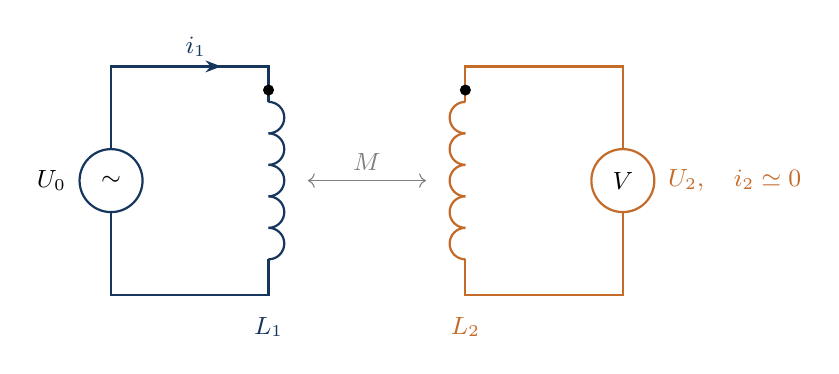
\begin{tikzpicture}
  \draw[ink,thick] (0,.4)--(0,1.45)--(2,1.45)--(2,1);
  \draw[ink,thick] (0,-.4)--(0,-1.45)--(2,-1.45)--(2,-1);
  \draw[ink,thick] (0,0) circle (.4);\node at (0,0) {$\sim$};
  \node[left] at (-.45,0) {$U_0$};
  \foreach \y in {-1,-.6,-.2,.2,.6}{\draw[ink,thick] (2,\y) arc (-90:90:.2);}
  \foreach \y in {1,.6,.2,-.2,-.6}{\draw[force,thick] (4.5,\y) arc (90:270:.2);}
  \draw[force,thick] (4.5,1)--(4.5,1.45)--(6.5,1.45)--(6.5,.4);
  \draw[force,thick] (4.5,-1)--(4.5,-1.45)--(6.5,-1.45)--(6.5,-.4);
  \draw[force,thick] (6.5,0) circle (.4);\node at (6.5,0) {$V$};
  \fill (2,1.15) circle (2pt);\fill (4.5,1.15) circle (2pt);
  \draw[vec,ink] (.75,1.45)--(1.4,1.45) node[midway,above] {$i_1$};
  \node[ink] at (2,-1.86) {$L_1$};\node[force] at (4.5,-1.86) {$L_2$};
  \draw[<->,gray] (2.5,0)--(4,0) node[midway,above] {$M$};
  \node[force,right] at (6.95,0) {$U_2,\quad i_2\simeq0$};
\end{tikzpicture}
\end{document}
